% Run 3 dilepton trigger efficiency and scale factor AN
% Skeleton based on the structure/style of the CPV AN.

%%%%%%%%%%%%% local definitions %%%%%%%%%%%%%%%%%%%%%
\newcommand{\physrev}   {Phys. Rev.\xspace}
\newcommand{\npion}   {$\pi ^{0}$}
%\newcommand{\ttbar}     {$t\overline{t}$\xspace}
\newcommand{\dilepton}  {$t\overline{t}_{dilepton}$\xspace}
%\newcommand{\bbbar}     {\mbox{$b\bar{b}$}\xspace}
%\newcommand{\ccbar}     {\mbox{$c\bar{c}$}\xspace}
\newcommand{\ppbar}     {\mbox{$p\bar{p}$}\xspace}
\newcommand{\herwig}    {\sc{herwig}}
\newcommand{\pythia}    {\sc{pythia}}
\newcommand{\vecbos}    {\sc{vecbos}}
\newcommand{\alpgen}    {\sc{alpgen}}
\newcommand{\qq}        {\sc{qq}}
\newcommand{\evtgen}    {\sc{evtgen}}
\newcommand{\tauola}    {\sc{tauola}}
\newcommand{\geant}     {\sc{geant}}
\newcommand{\met}       {\mbox{$\not\!\!E_T$}\xspace}
\newcommand{\metcal}    {\mbox{$\not\!\!E_{Tcal}$}\xspace}
\newcommand{\rar}       {\rightarrow}
\newcommand{\eps}       {\epsilon}
\newcommand{\wplus}     {$W+$jets\xspace}
\newcommand{\zplus}     {$Z+$jets\xspace}
\newcommand{\wplusfour} {$W+$4jets\xspace}
\newcommand{\qcdplus}   {QCD-multijets\xspace} 
\newcommand{\kapa}      {MC-to-data correction factor\xspace}
\newcommand{\kapas}     {MC-to-data correction factors\xspace}
\newcommand{\Ztautau}   {$Z\to\tau\tau$\xspace}
\newcommand{\Zmumu}     {$Z\to\mu\mu$\xspace}
\newcommand{\Zee}       {$Z\to ee$\xspace}
\newcommand{\lowmet}    {low-\mbox{$\not\!\!E_T$}-QCD\xspace}
\newcommand{\muplus}    {$\mu+$jets\xspace}
\newcommand{\eplus}     {$e+$jets\xspace}
\newcommand{\lplus}     {lepton+jets\xspace}
%\newcommand{\MET}       {$\not\!\!E_T$}
\newcommand{\wrt}       {with respect to\xspace}
\newcommand{\lminust}   {{\bf L-T} \xspace}
%\newcommand{\pt}        {\mbox{$p_{\rm T}$}}
\newcommand{\comphep}   {\sc{c}\rm{omp}\sc{hep}}
\newcommand{\singletop} {\sc{s}\rm{ingle}\sc{t}\rm{op}}
\newcommand{\wetc}      {$W$\bbbar+$W$\ccbar+$Wjj$ \xspace}
\newcommand{\ee} {$e^+e^-$}
\newcommand{\mumu} {$\mu^{+}\mu^{-}$}
\newcommand{\emu} {$e^{\pm}\mu^{\mp}$}
\newcommand{\bjet} {$b$-quark jet}
\newcommand{\bjets} {$b$-quark jets}
\newcommand{\oone} {$\mathcal{O}_{1}$}
\newcommand{\othree} {$\mathcal{O}_{3}$}
\newcommand{\mex} {\ensuremath{E\!\!\!\!/_\text{x}}}
\newcommand{\mey} {\ensuremath{E\!\!\!\!/_\text{y}}}
\newcommand{\px}{\ensuremath{p_\text{x}}{}}
\newcommand{\py}{\ensuremath{p_\text{y}}{}}
\newcommand{\pz}{\ensuremath{p_\text{z}}{}}

%%%%%%%%%%%%% local definitions %%%%%%%%%%%%%%%%%%%%%

% --- Observables and Asymmetries (New definitions) ---
\providecommand{\ObsOne}{\ensuremath{\mathcal{O}_{1}}\xspace}
\providecommand{\ObsThree}{\ensuremath{\mathcal{O}_{3}}\xspace}
\providecommand{\ObsInd}{\ensuremath{\mathcal{O}_{i}}\xspace}
\providecommand{\AsymI}{\ensuremath{\text{A}_{\mathcal{O}_{i}}}\xspace}
\providecommand{\AsymOne}{\ensuremath{\text{A}_{\mathcal{O}_{1}}}\xspace}
\providecommand{\AsymThree}{\ensuremath{\text{A}_{\mathcal{O}_{3}}}\xspace}

% --- CEDM and Lagrangian Parameters ---
\providecommand{\dtG}{\ensuremath{d_{\PQt G}}\xspace}
\providecommand{\ImdtG}{\ensuremath{\text{Im}(\dtG)}\xspace}
\providecommand{\Lag}{\ensuremath{\mathcal{L}}\xspace}
\providecommand{\gS}{\ensuremath{g_{\mathrm{S}}}\xspace}
\providecommand{\GMM}{\ensuremath{T^a}\xspace}
\providecommand{\FST}{\ensuremath{G_{\mu\nu}}\xspace}
\providecommand{\CMDM}{\ensuremath{a^{\Pg}_{\PQt}}\xspace}

% --- Particles and Kinematics (Using providecommand to avoid conflicts) ---
\providecommand{\PQt}{\text{t}\xspace}
\providecommand{\PAQt}{\bar{\text{t}}\xspace}
\providecommand{\PQb}{\text{b}\xspace}
\providecommand{\PAQb}{\bar{\text{b}}\xspace}
\providecommand{\Pellp}{\ell^{+}\xspace}
\providecommand{\Pellm}{\ell^{-}\xspace}
\providecommand{\Pellpm}{\ell^{\pm}\xspace}

\providecommand{\momt}{\ensuremath{p_{\PQt}}\xspace}
\providecommand{\momat}{\ensuremath{p_{\PAQt}}\xspace}
\providecommand{\momb}{\ensuremath{p_{\PQb}}\xspace}
\providecommand{\momab}{\ensuremath{p_{\PAQb}}\xspace}
\providecommand{\momlp}{\ensuremath{p_{\Pellp}}\xspace}
\providecommand{\momlm}{\ensuremath{p_{\Pellm}}\xspace}

% --- Units and Symbols ---
\providecommand{\TeV}{\,\text{TeV}\xspace}
\providecommand{\fbinv}{\,\text{fb}^{-1}\xspace}
\providecommand{\trigSF}{\ensuremath{\mathrm{SF}_{\mathrm{trig}}}\xspace}


%%%%%%%%%%%%% local definitions %%%%%%%%%%%%%%%%%%%%%


% Visible placeholders for analysis inputs and results still in progress.
\newcommand{\todo}[1]{\textbf{[TO VERIFY: #1]}}
\newcommand{\insertitem}[1]{\textbf{[TO INSERT: #1]}}
\newcommand{\plotplaceholder}[1]{\fbox{\begin{minipage}[c][3.2cm][c]{0.83\linewidth}\centering\small\textbf{Result plot pending}\\#1\end{minipage}}}

%%%%%%%%%%%%%%% Title page %%%%%%%%%%%%%%%%%%%%%%%%
\cmsNoteHeader{AN-26-XXX}
\title{Measurement of dilepton trigger efficiencies and scale factors with the Run 3 dataset}

% >> Authors
%Author is always "The CMS Collaboration" for PAS and papers, so author, etc, below will be ignored in those cases
%For multiple affiliations, create an address entry for the combination
%To mark authors as primary, use the \author* form
\address[inst1]{Korea University (KR)}
\author[inst1]{Haeyun Hwang}
\author[inst1]{Seungkyu Ha}
\author[inst1]{Jae Hyeok Yoo}
\address[inst2]{Kyungpook National University}
\author[inst2]{Sehwook Lee}
\author[inst2]{Junghyun Lee}
\author[inst2]{Gyeongmo Kim}
\address[inst3]{Yonsei University}
\author[inst3]{Guk Cho}
\author[inst3]{Dongwoon Kim}
\author[inst3]{Hwi Dong Yoo}


% Add collaborators as needed.

\date{\today}

\abstract{
The trigger efficiencies and corresponding data-to-simulation scale factors are to be measured for events containing two oppositely charged leptons using proton--proton collision data collected by the CMS experiment during Run 3 at a center-of-mass energy of $13.6~\TeV$. The measurement is performed separately in the $ee$, $e\mu$, and $\mu\mu$ final states. The measurement is motivated by the Run 3 extension of the $\ttbar$ CP violation analysis in the dilepton channel and can also be used by other top quark analyses with similar final states. The trigger efficiencies are measured using an independent set of missing transverse momentum triggers. The scale factors are to be obtained from the ratio of the efficiencies measured in data and simulation, and their dependence on lepton kinematic properties, pileup, and event topology is investigated.
}

\hypersetup{
  pdfauthor={Seungkyu Ha, Dongwoon Kim, Haeyun Hwang, Jae Hyeok Yoo, Sehwook Lee, Junghyun Lee, Gyeongmo Kim, Guk Cho, Hwi Dong Yoo},
  pdftitle={Measurement of dilepton trigger efficiencies and scale factors with the Run 3 dataset},
  pdfsubject={CMS Analysis Note},
  pdfkeywords={CMS, top quark, ttbar, dilepton, trigger, efficiency, scale factor, Run 3}
}

\maketitle
\tableofcontents

%% body
\section{Introduction}\label{sec:intro}
Accurate modelling of the trigger response is required for dileptonic top-quark measurements. The efficiency of the analysis trigger OR is measured in data and simulated events selected with MET reference triggers. Their ratio defines the event-level trigger correction. The present note documents the Run 3 measurement. This draft currently presents the supplied 2024 and 2025 results for $ee$, $e\mu$, and $\mu\mu$, motivated by the top-quark CP-violation analysis. A previous CMS search studied CP-violating top quark couplings in dilepton events at 13~TeV~\cite{TOP18007}.
The MET-reference strategy follows the approach described in the earlier Run 2 trigger study~\cite{run2}. The existing Run 3 draft~\cite{earlier} supplies the provisional trigger and offline-selection descriptions. Numerical results shown here come from the supplied 2024 and 2025 plot sets; their inclusion does not independently establish that the provisional selection matches the production configuration.

The 2024 and 2025 results are reported separately; results for 2022 and 2023 will be added in subsequent updates.

\section{Data and simulation}\label{sec:data}
The measurement uses separate 2024 and 2025 datasets at $\sqrt{s}=13.6$~TeV.
The supplied one-dimensional plots are labelled with integrated luminosities of $109.82~\mathrm{fb}^{-1}$ for 2024 and $110.37~\mathrm{fb}^{-1}$ for 2025.
These values are retained as the measurement figure metadata; they are not replaced by luminosities quoted for different analysis selections or input versions.
The reference data are collected with MET/JetMET triggers, and dileptonic $t\bar t$ simulation provides the simulated reference.
The two years are kept separate in the result figures and correction lookup.
The supplied files \texttt{TriggerSF\_2024.root} and \texttt{TriggerSF\_2025.root} are distributed unchanged.
\todo{Confirm the actual data and MC input lists, campaign, certified run intervals, luminosity calculation, and dataset-overlap removal for each year.}

\section{Trigger paths}\label{sec:triggers}
For each final state, the signal-trigger decision is the logical OR of the applicable single-lepton and dilepton paths. Table~\ref{tab:signal} lists the Run 3 signal paths; every path must be checked against the HLT menu and NanoAOD branches in each period. A recorded event may pass several paths but enters each numerator once. Any run-dependent changes, prescales, dataset-overlap removal, or trigger-object matching requirements must be documented before finalization.
\begin{table}[htbp]\centering\small
\caption{Signal-trigger OR used for the dilepton trigger measurement. Path suffixes \texttt{\_v*} are suppressed. Confirm per-era availability and signal dataset overlap removal.}\label{tab:signal}
\begingroup
\renewcommand{\arraystretch}{1.25}
\begin{tabular}{@{}p{0.12\linewidth}p{0.83\linewidth}@{}}\hline
Channel & Signal HLT path \\\hline
\multirow{3}{*}{$ee$} & {\footnotesize\path{HLT_Ele23_Ele12_CaloIdL_TrackIdL_IsoVL}} \\
 & {\footnotesize\path{HLT_Ele32_WPTight_Gsf}} \\
 & {\footnotesize\path{HLT_DoubleEle25_CaloIdL_MW}} \\
\hline
\multirow{5}{*}{$e\mu$} & {\footnotesize\path{HLT_Mu23_TrkIsoVVL_Ele12_CaloIdL_TrackIdL_IsoVL}} \\
 & {\footnotesize\path{HLT_Mu8_TrkIsoVVL_Ele23_CaloIdL_TrackIdL_IsoVL_DZ}} \\
 & {\footnotesize\path{HLT_Mu12_TrkIsoVVL_Ele23_CaloIdL_TrackIdL_IsoVL_DZ}} \\
 & {\footnotesize\path{HLT_Ele32_WPTight_Gsf}} \\
 & {\footnotesize\path{HLT_IsoMu24}} \\
\hline
\multirow{2}{*}{$\mu\mu$} & {\footnotesize\path{HLT_Mu17_TrkIsoVVL_Mu8_TrkIsoVVL_DZ_Mass3p8}} \\
 & {\footnotesize\path{HLT_IsoMu24}} \\
\hline
\end{tabular}\endgroup
\end{table}
\subsection{MET reference triggers}\label{sec:reference}
Events for the efficiency denominator are recorded with a logical OR of MET or MET+HT reference paths. These triggers select events without directly requiring an electron or muon. The candidate reference set is given in Table~\ref{tab:met}. The unprescaled status and validity interval of each path, and its actual NanoAOD implementation, must be verified. The MET requirement of the reference trigger can bias the measured efficiency if it is correlated with the dilepton trigger; this assumption is examined in Section~\ref{sec:corr}.
\begin{table}[htbp]\centering\small
\caption{Candidate MET-reference paths. Their availability must be verified separately for each 2025 period. Preserve only paths verified in each run and in the input files.}\label{tab:met}
\begingroup
\renewcommand{\arraystretch}{1.25}
\begin{tabular}{@{}p{0.25\linewidth}p{0.70\linewidth}@{}}\hline
Reference category & HLT path \\\hline
\multirow{2}{*}{MET} & {\footnotesize\path{HLT_PFMET120_PFMHT120_IDTight}} \\
 & {\footnotesize\path{HLT_PFMET200_BeamHaloCleaned}} \\
\hline
Type-1 MET & {\footnotesize\path{HLT_PFMETTypeOne200_BeamHaloCleaned}} \\
\hline
MET (no muons) & {\footnotesize\path{HLT_PFMETNoMu120_PFMHTNoMu120_IDTight}} \\
\hline
MET + HT & {\footnotesize\path{HLT_PFMET120_PFMHT120_IDTight_PFHT60}} \\
\hline
MET (no muons) + HT & {\footnotesize\path{HLT_PFMETNoMu120_PFMHTNoMu120_IDTight_PFHT60}} \\
\hline
\multirow{4}{*}{HT + MET} & {\footnotesize\path{HLT_PFHT500_PFMET100_PFMHT100_IDTight}} \\
 & {\footnotesize\path{HLT_PFHT700_PFMET85_PFMHT85_IDTight}} \\
 & {\footnotesize\path{HLT_PFHT800_PFMET75_PFMHT75_IDTight}} \\
 & {\footnotesize\path{HLT_PFHT500_PFMET110_PFMHT110_IDTight}} \\
\hline
MET (no muons), HF & {\footnotesize\path{HLT_PFMETNoMu120_PFMHTNoMu120_IDTight_FilterHF}} \\
\hline\end{tabular}
\endgroup
\end{table}

\section{Object and event selection}\label{sec:selection}
The selection follows the earlier Run 3 trigger-AN draft~\cite{earlier}, adapted to the nominal CPV analysis choices of a medium UParT $b$-tagging working point and a run-dependent Jet Veto Map. The same offline selection is applied to data and simulation where applicable. Table~\ref{tab:sel} summarizes the numerical cuts specified in that draft. Identification working points, year-dependent calibrations and trigger-study input code require a final cross-check before this selection is presented as the implemented measurement.
\subsection{Electron selection}\label{sec:electron}
Electrons have $p_{\mathrm T}>15~\mathrm{GeV}$ and $|\eta|<2.4$. Those in the ECAL barrel--endcap transition region are excluded. The nominal electron identification, isolation, momentum calibration and overlap-removal criteria follow the CPV reconstruction. \todo{Specify the exact ECAL gap, identification and isolation working points, impact-parameter cuts, correction versions and period dependence from the Run 3 code.}
\subsection{Muon selection}\label{sec:muon}
Muons have $p_{\mathrm T}>15~\mathrm{GeV}$ and $|\eta|<2.4$ and pass the nominal CPV identification and isolation. Momentum corrections and overlap removal are applied consistently to data and simulation. \todo{Specify exact ID, isolation and impact-parameter criteria and correction version.}
\subsection{Jet selection}\label{sec:jet}
Jets are clustered with the anti-$k_{\mathrm T}$ algorithm with radius $R=0.4$ from PUPPI-weighted particle-flow candidates. Selected jets satisfy $p_{\mathrm T}>30~\mathrm{GeV}$, $|\eta|<2.4$, the recommended jet ID, and lepton cleaning. Run-dependent JEC and JER treatments are applied. The recommended period-specific Jet Veto Map is applied according to its prescription in data and simulation. \todo{Confirm jet ID, cleaning radius, JEC/JER versions, veto-map identifiers and event-versus-jet veto logic.}
\subsection{$b$ jet identification}\label{sec:btag}
At least one selected jet must pass the \emph{medium} Unified Particle Transformer (UParT) $b$-tagging working point. This is distinct from alternative medium \emph{object selections} in Appendix~\ref{app:alternatives}. \todo{Insert per-period UParT branch and thresholds, calibration, and availability in each NanoAOD campaign.}
\subsection{Missing transverse momentum}\label{sec:met}
PUPPI missing transverse momentum is used. The earlier Run 3 draft~\cite{earlier} imposes $p_{\mathrm T}^{\mathrm{miss}}>100~\mathrm{GeV}$, on both efficiency numerator and denominator. The recommended event filters and propagated object corrections are applied. \todo{Confirm the 100~GeV cut, PUPPI MET branch, filter list, and consistency with the final CPV selection and reference-trigger plateau.}
\subsection{Event selection}\label{sec:events}
Events contain at least two oppositely charged selected leptons in an exclusive $ee$, $e\mu$, or $\mu\mu$ channel. The leading and subleading leptons satisfy $p_{\mathrm T}>25$ and $15~\mathrm{GeV}$, respectively, and $m_{\ell\ell}>20~\mathrm{GeV}$. At least one selected jet passes medium UParT, and $p_{\mathrm T}^{\mathrm{miss}}>100~\mathrm{GeV}$ is required. Recommended quality filters and the Jet Veto Map are applied. The earlier draft does not establish an exact-two-lepton veto, a minimum total jet multiplicity, or a same-flavour $Z$ veto; add these only if implemented in the Run 3 trigger study.
\begin{table}[htbp]\centering\small
\caption{Draft nominal offline selection from the earlier trigger AN~\cite{earlier} and the agreed UParT-medium and Jet Veto Map choices. Exact working points require code verification.}\label{tab:sel}
\begin{tabular}{p{0.32\linewidth}p{0.58\linewidth}}\hline
Object or quantity & Requirement \\\hline
Electrons & $p_{\mathrm T}>15~\mathrm{GeV}$, $|\eta|<2.4$; ECAL transition veto; CPV ID and isolation.\\
Muons & $p_{\mathrm T}>15~\mathrm{GeV}$, $|\eta|<2.4$; CPV ID and isolation.\\
AK4 PUPPI jets & $p_{\mathrm T}>30~\mathrm{GeV}$, $|\eta|<2.4$; jet ID and lepton cleaning.\\
Jet Veto Map & Recommended period-specific map applied.\\
Dilepton topology & $\geq2$ opposite-charge leptons in $ee$, $e\mu$, $\mu\mu$; leading (subleading) $p_{\mathrm T}>25$ ($15$) GeV; $m_{\ell\ell}>20~\mathrm{GeV}$.\\
$b$-tagged jets & $\geq1$ selected jet at UParT medium working point.\\
PUPPI missing momentum & $p_{\mathrm T}^{\mathrm{miss}}>100~\mathrm{GeV}$.\\
Event quality & Period-specific filters and certified data lumisections.\\\hline
\end{tabular}\end{table}
For the efficiency measurement, the MET-reference trigger is imposed on numerator and denominator; the signal trigger is imposed only on the numerator. \todo{Check the table against final code and document year- or channel-dependent deviations.}

\section{Efficiency and scale-factor measurement}\label{sec:method}
Let $O$ denote the offline event selection, $R$ the reference-trigger OR, and $S_c$ the signal-trigger OR for channel $c$. The measured efficiency in bin $i$ is
\begin{equation}\label{eq:eff}
\widehat\epsilon_{d/m,c,i}=\frac{N_{d/m,c,i}(O\cap R\cap S_c)}{N_{d/m,c,i}(O\cap R)},\qquad
\mathrm{SF}_{c,i}=\frac{\widehat\epsilon_{d,c,i}}{\widehat\epsilon_{m,c,i}}.
\end{equation}
The numerator is a subset of the denominator. Each event enters once even when multiple signal paths fire. Simulation counts represent the configured sum of non-trigger weights; the same weights are applied in the numerator and denominator. The conditional efficiency $P(S_c\mid O,R)$ represents $P(S_c\mid O)$ only when the residual reference-trigger bias is controlled.
The supplied one-dimensional figures already combine data and MC efficiencies with their SF ratio. These are used directly in the main results; selected numerator, denominator, and efficiency diagnostics are provided in Appendix~\ref{app:2024-support} and Appendix~\ref{app:2025-support-2025}. The leading/subleading convention is used in one-dimensional plots. For the final two-dimensional correction, same-flavour leptons are ordered by transverse momentum, whereas the mixed-flavour map uses $x=p_{\mathrm T}^{e}$ and $y=p_{\mathrm T}^{\mu}$.
The lowest occupied bins probe the turn-on region and should not be described as plateau bins without checking the offline thresholds and trigger response. Invalid, unpopulated, and inaccessible bins must not be assigned unity by default.\todo{Verify interval construction, MC weight treatment, exact bin edges, and underflow/overflow rules from code.}

\section{Uncertainties}\label{sec:unc}
\subsection{Statistical precision}
The numerator--denominator covariance must be retained when estimating efficiency errors. For data this requires a binomial construction where applicable; weighted simulation requires a treatment appropriate to its weights, including any negative weights. The supplied statistical and breakdown plots are retained without attributing an unverified interval algorithm to them.
\subsection{Topology, pileup and era dependence}
The supplied legends define jet-multiplicity regions $N_{\mathrm{jet}}<3$ and $N_{\mathrm{jet}}\geq3$, and vertex regions $N_{\mathrm{PV}}<40$ and $N_{\mathrm{PV}}\geq40$. These boundaries supersede the different provisional jet split in the original draft. The breakdown legends describe an envelope relative to the nominal SF. The intended interpretation is
\begin{equation}
\delta_k(i)=\max_{a\in\{\mathrm{low,high}\}}|\mathrm{SF}_{k,a}(i)-\mathrm{SF}_{\mathrm{nom}}(i)|,
\end{equation}
with relative uncertainty obtained by division by $|\mathrm{SF}_{\mathrm{nom}}(i)|$. This interpretation, including any statistical subtraction, must be checked against the production code. An era-dependence component is also shown; the plot alone does not specify its luminosity weighting or combination procedure.
\subsection{Reference--signal correlation}\label{sec:corr}
A useful diagnostic is
\begin{equation}
\alpha_c=\frac{P(R\cap S_c\mid O)}{P(R\mid O)P(S_c\mid O)},\qquad P(S_c\mid O,R)=\alpha_c P(S_c\mid O).
\end{equation}
Thus the reference-conditioned SF differs from the inclusive SF by $\alpha_d/\alpha_m$. An MC-only correlation study cannot determine this ratio in data without additional assumptions. The supplied orange curves are labelled as a correlation uncertainty, not as measurements of $\alpha$; they must not be relabelled as $\alpha$ distributions.
\subsection{Uncertainty combination and current limitation}
The supplied relative-breakdown legend defines total systematic uncertainty using era, jet multiplicity, and vertex multiplicity, and total uncertainty from statistics and that systematic term. Although a correlation curve is shown, it is absent from the stated systematic sum. This discrepancy requires resolution before adopting the total error or the accompanying 2D uncertainty maps. The draft reproduces the figures without changing their numerical content.
\subsubsection{2024 uncertainty breakdowns}
\begin{figure}[htbp]\centering
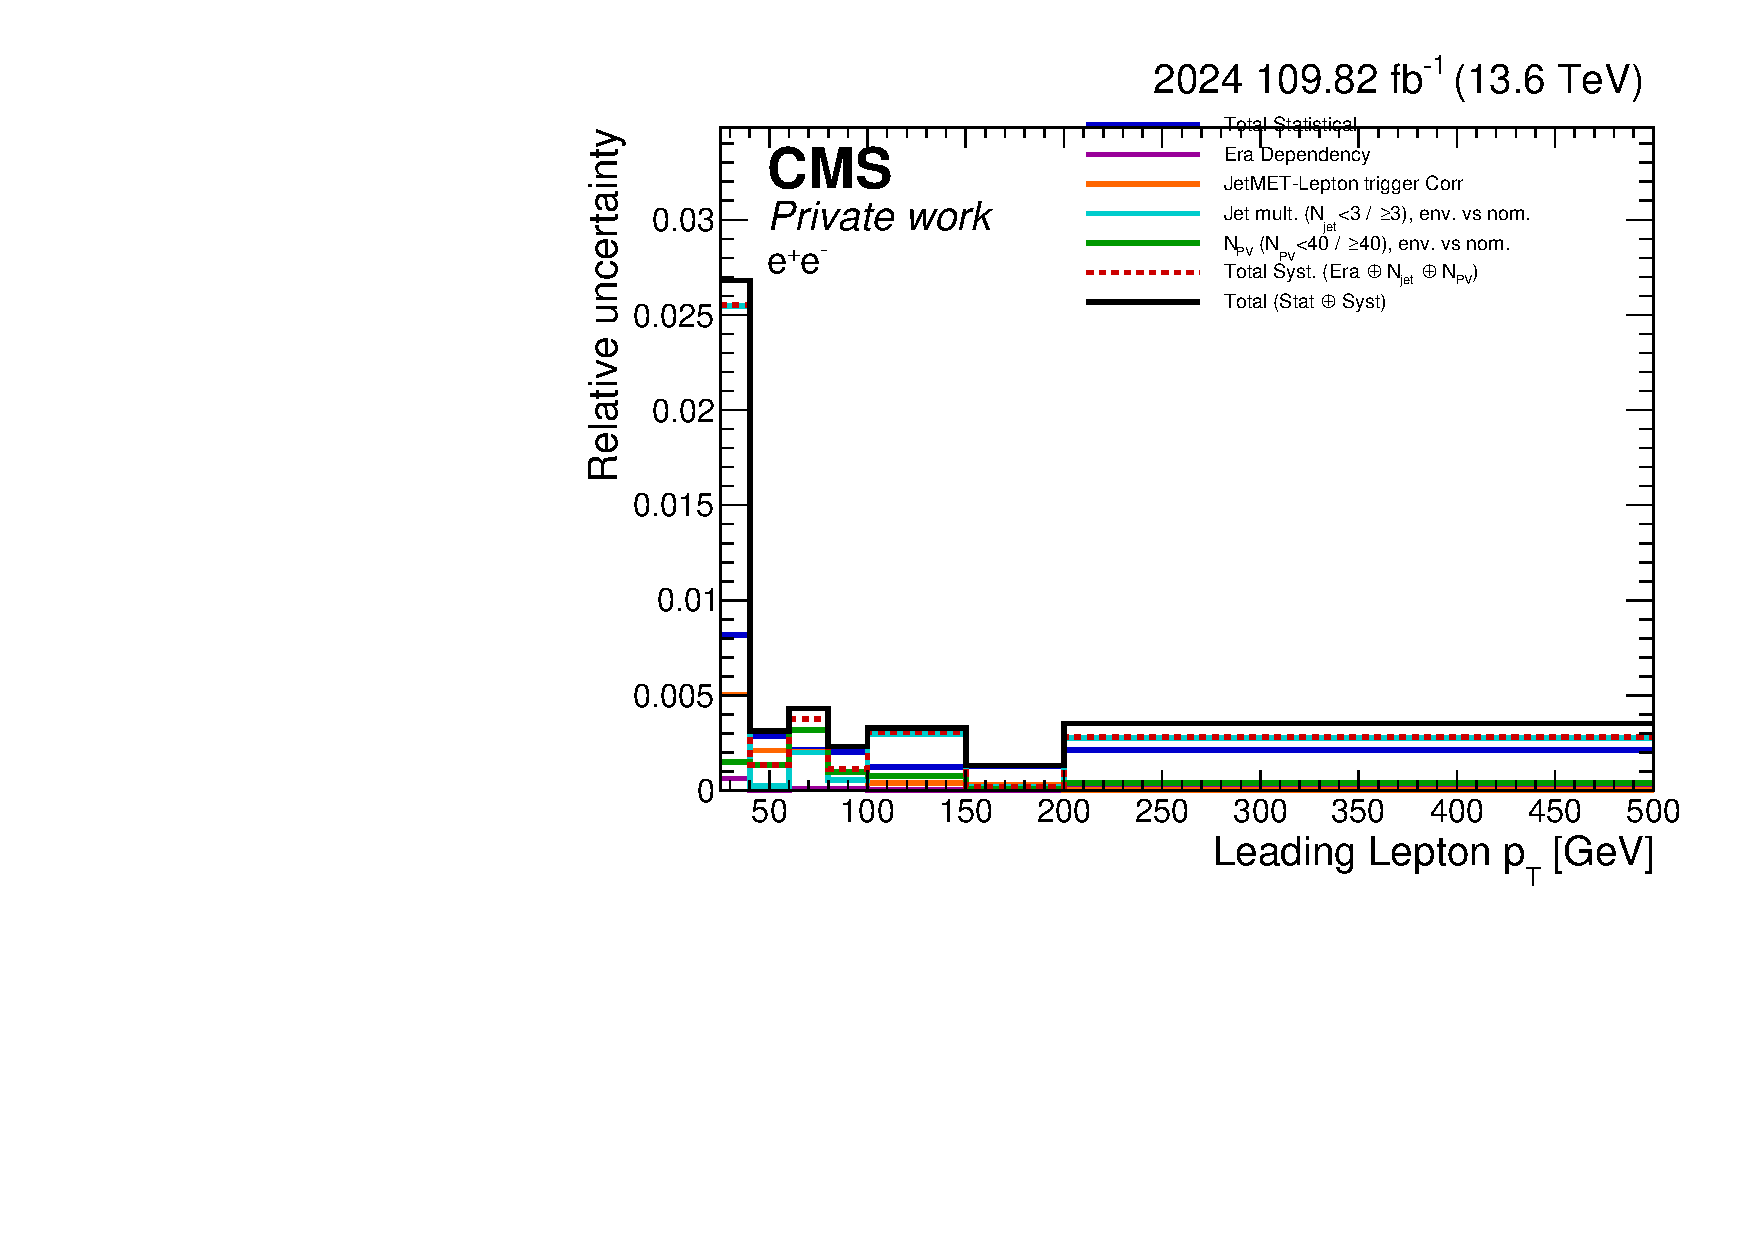
\includegraphics[width=0.48\linewidth]{figures/2024/ElEl/Relative_Uncertainty_Breakdown/Breakdown_Lep1pt.pdf}
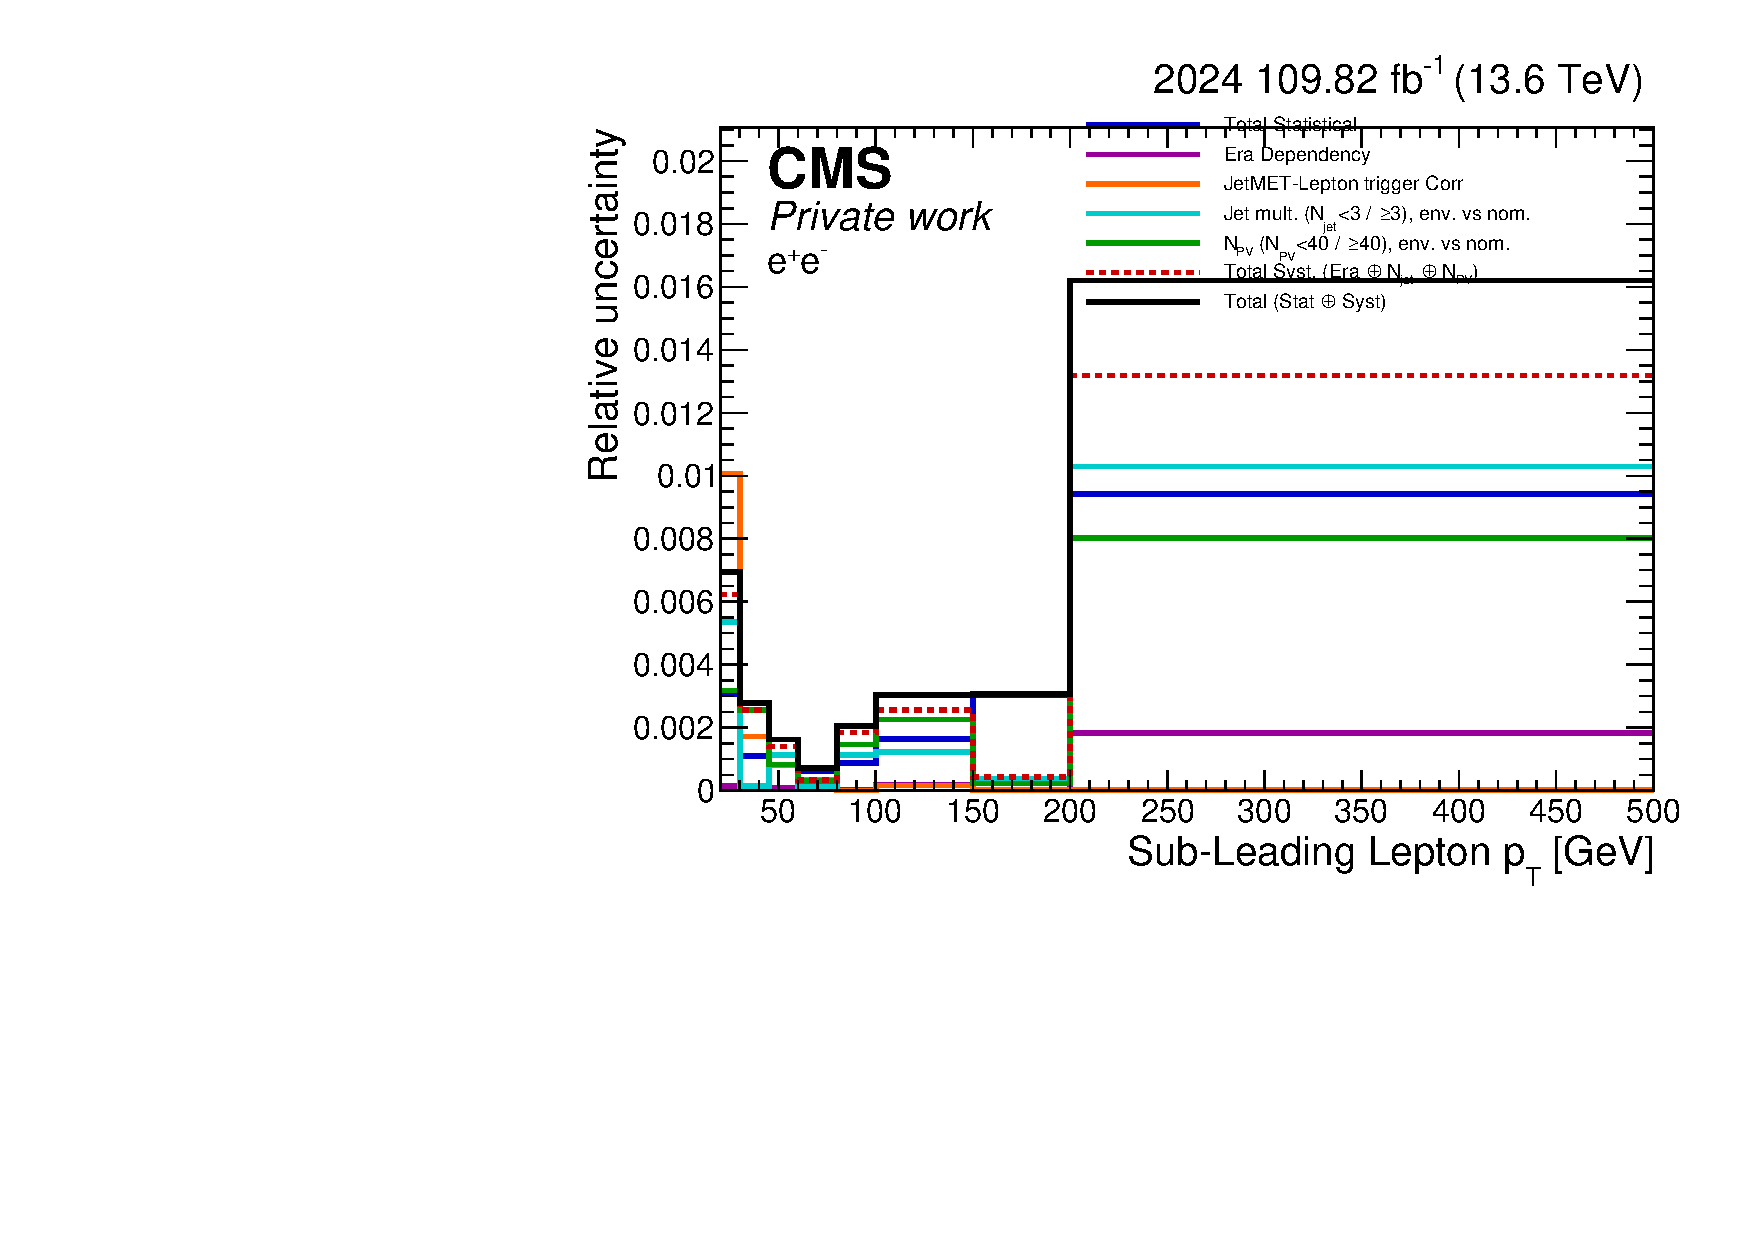
\includegraphics[width=0.48\linewidth]{figures/2024/ElEl/Relative_Uncertainty_Breakdown/Breakdown_Lep2pt.pdf}
\caption{2024: Relative uncertainty breakdown in the $ee$ channel versus leading and subleading lepton transverse momentum. The displayed total-systematic legend lists era, jet, and vertex components; the separately drawn correlation component is not listed in that sum.}\label{fig:unc-ElEl}
\end{figure}
\begin{figure}[htbp]\centering
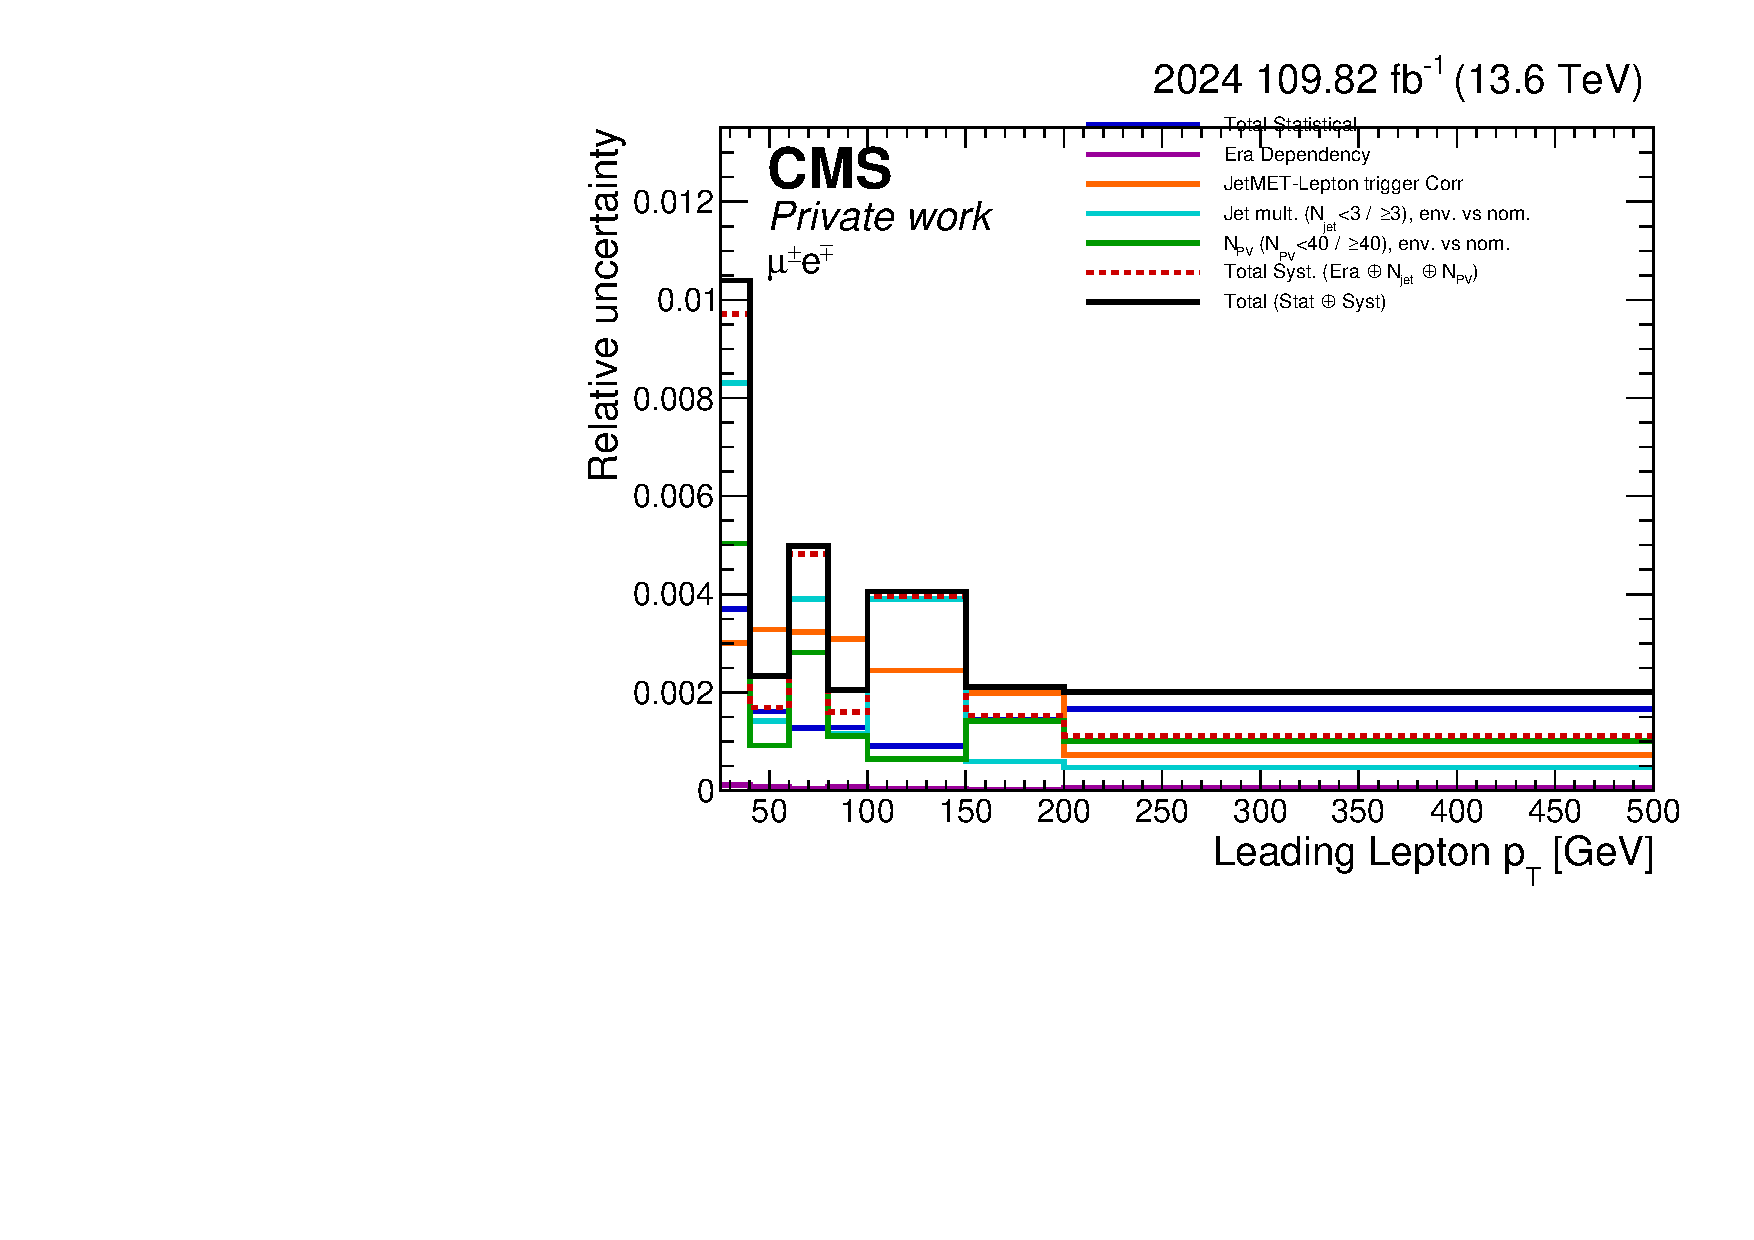
\includegraphics[width=0.48\linewidth]{figures/2024/MuEl/Relative_Uncertainty_Breakdown/Breakdown_Lep1pt.pdf}
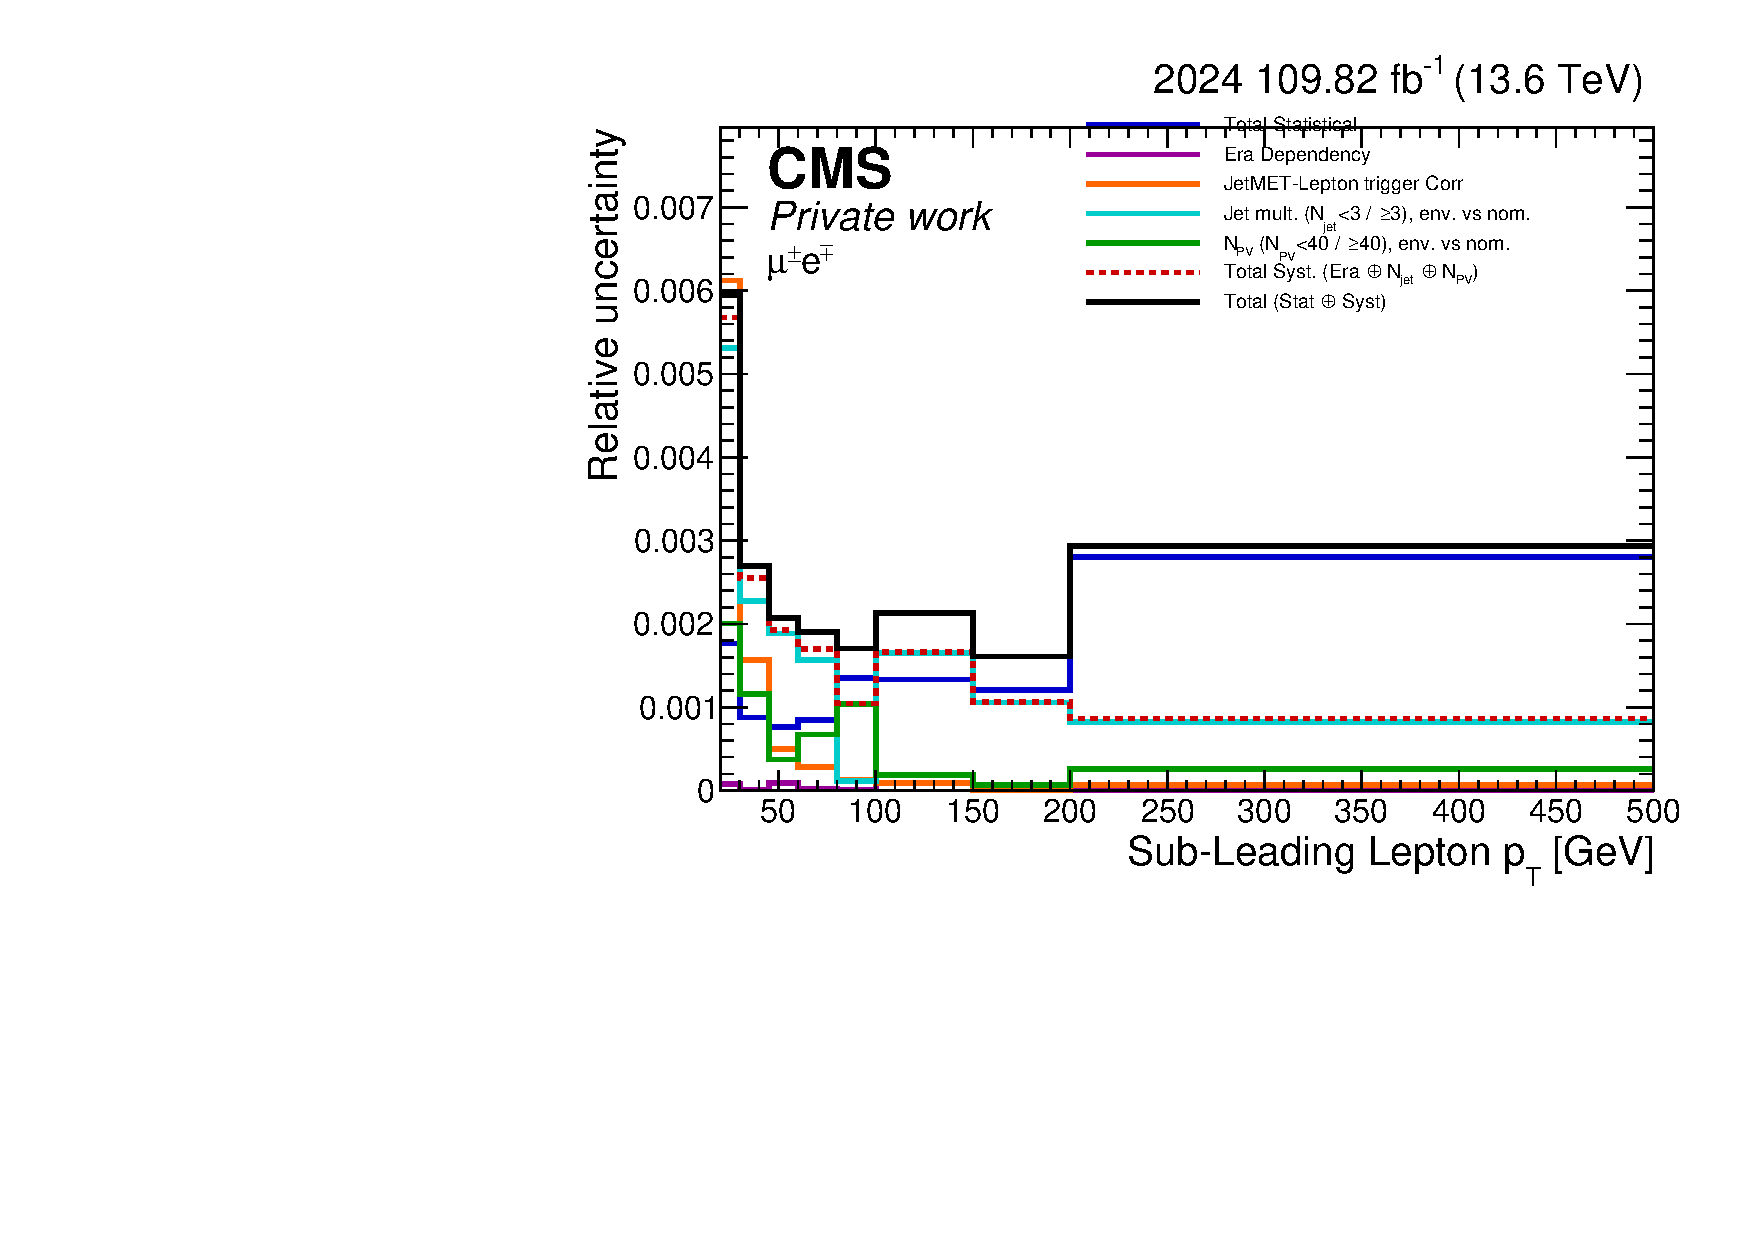
\includegraphics[width=0.48\linewidth]{figures/2024/MuEl/Relative_Uncertainty_Breakdown/Breakdown_Lep2pt.pdf}
\caption{2024: Relative uncertainty breakdown in the $e\mu$ channel versus leading and subleading lepton transverse momentum. The displayed total-systematic legend lists era, jet, and vertex components; the separately drawn correlation component is not listed in that sum.}\label{fig:unc-MuEl}
\end{figure}
\begin{figure}[htbp]\centering
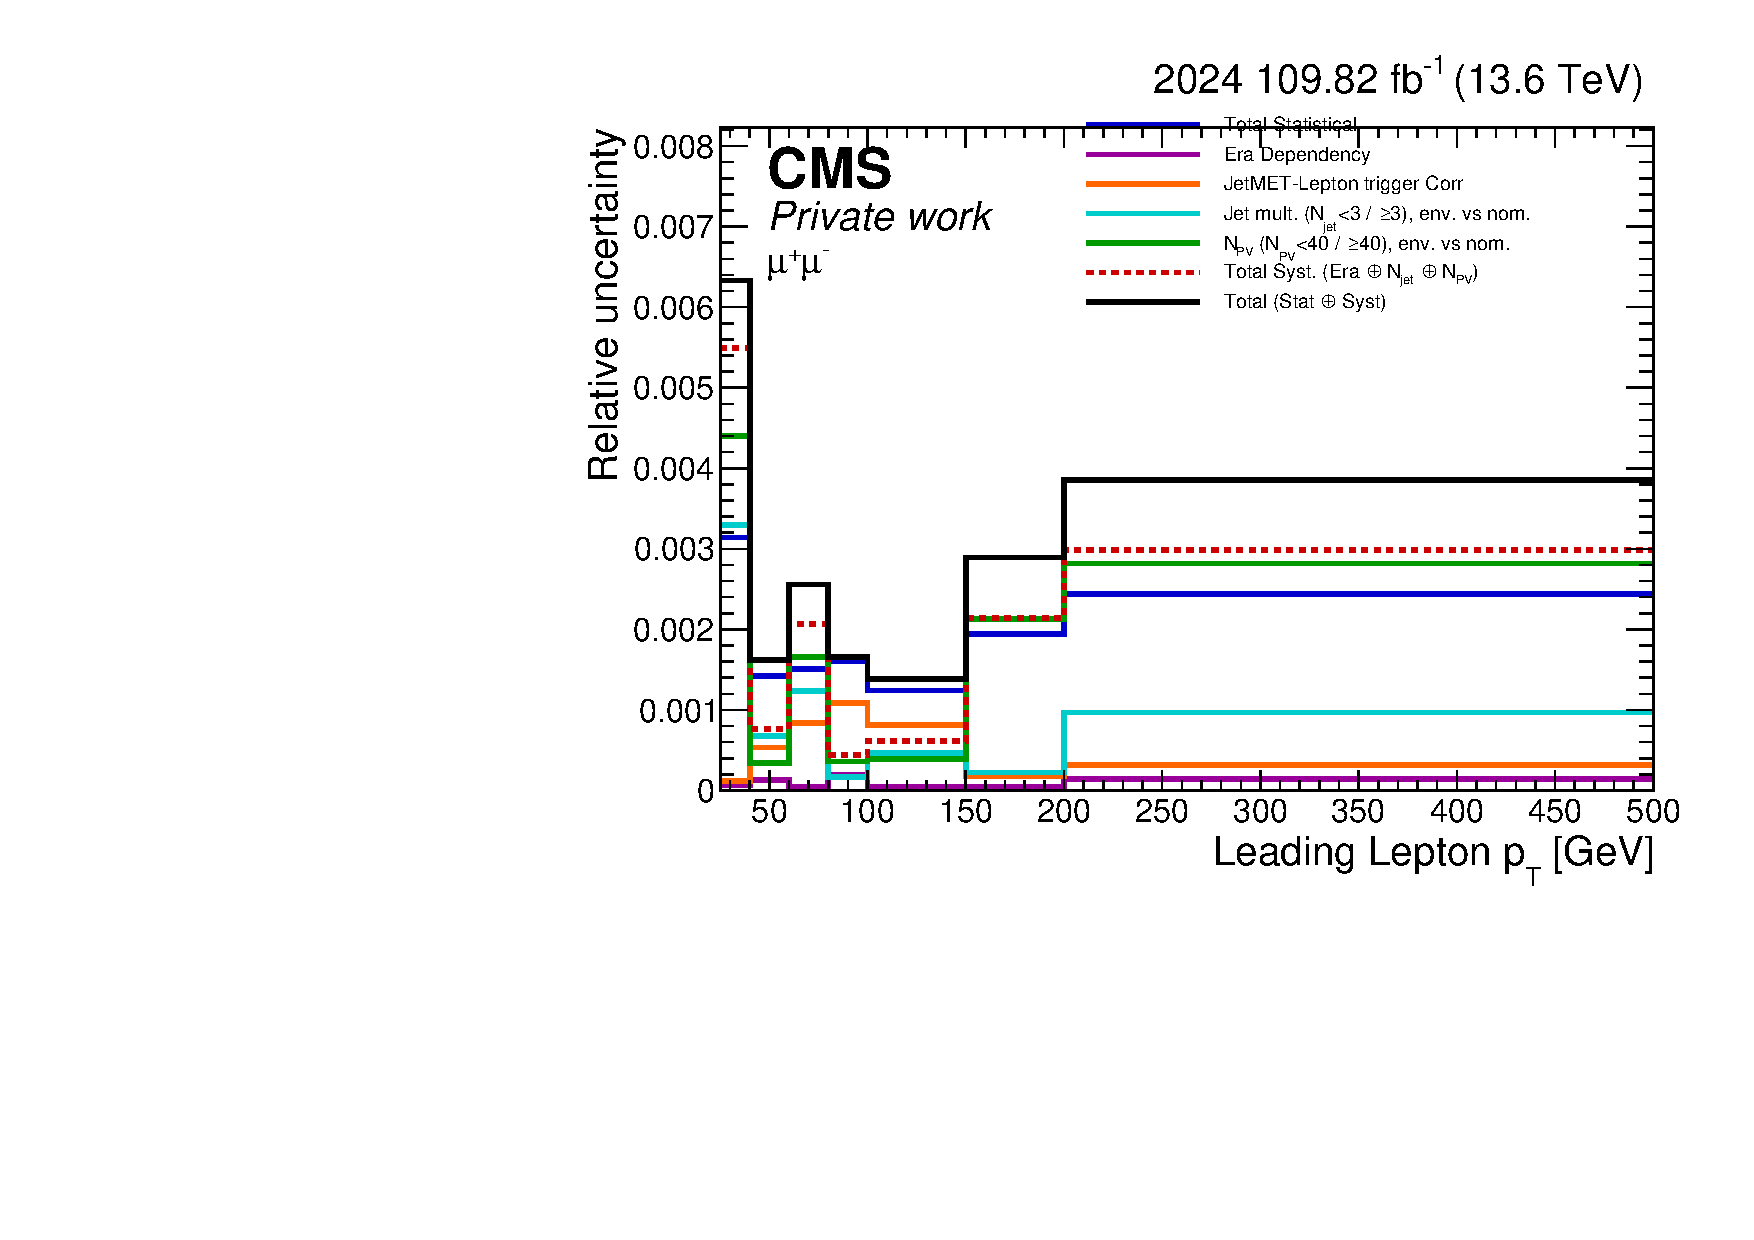
\includegraphics[width=0.48\linewidth]{figures/2024/MuMu/Relative_Uncertainty_Breakdown/Breakdown_Lep1pt.pdf}
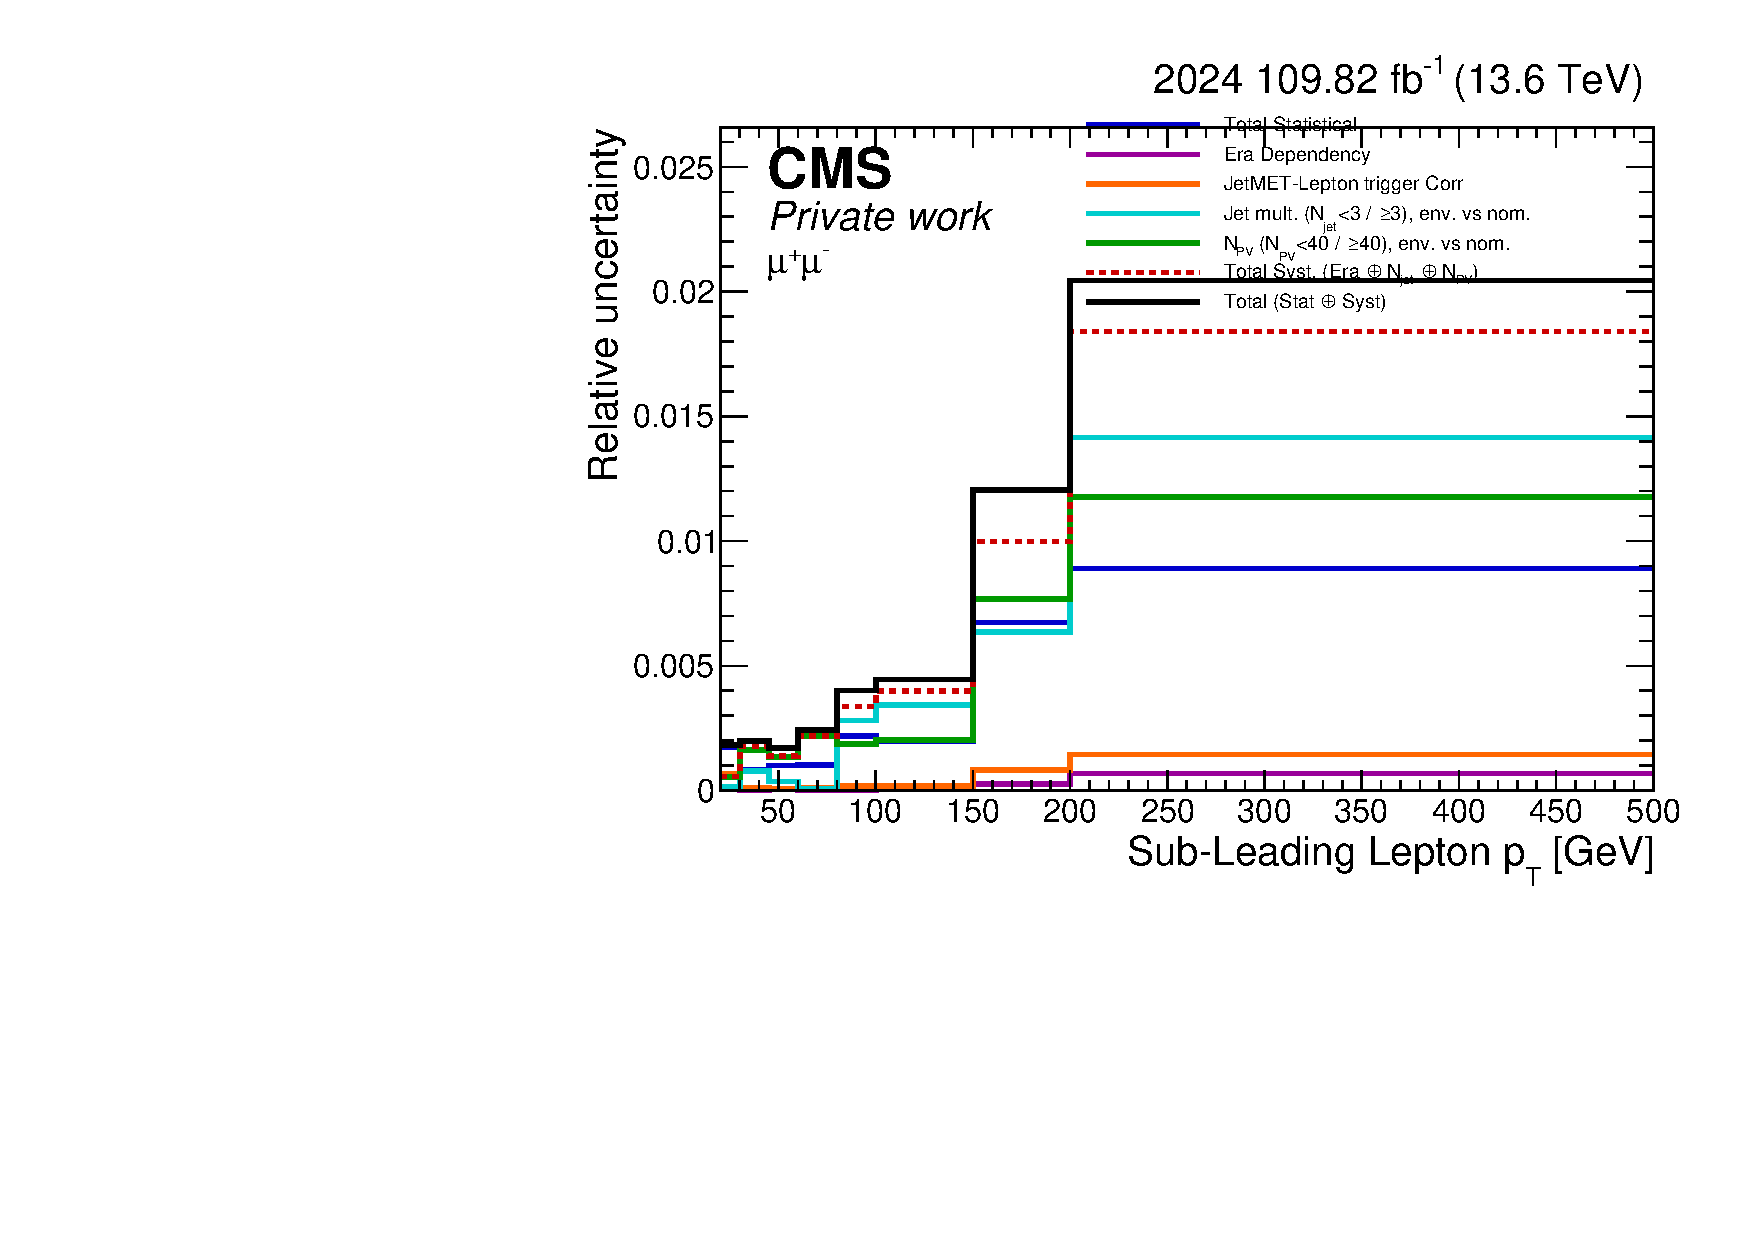
\includegraphics[width=0.48\linewidth]{figures/2024/MuMu/Relative_Uncertainty_Breakdown/Breakdown_Lep2pt.pdf}
\caption{2024: Relative uncertainty breakdown in the $\mu\mu$ channel versus leading and subleading lepton transverse momentum. The displayed total-systematic legend lists era, jet, and vertex components; the separately drawn correlation component is not listed in that sum.}\label{fig:unc-MuMu}
\end{figure}
\clearpage
\subsubsection{2025 uncertainty breakdowns}
\begin{figure}[htbp]\centering
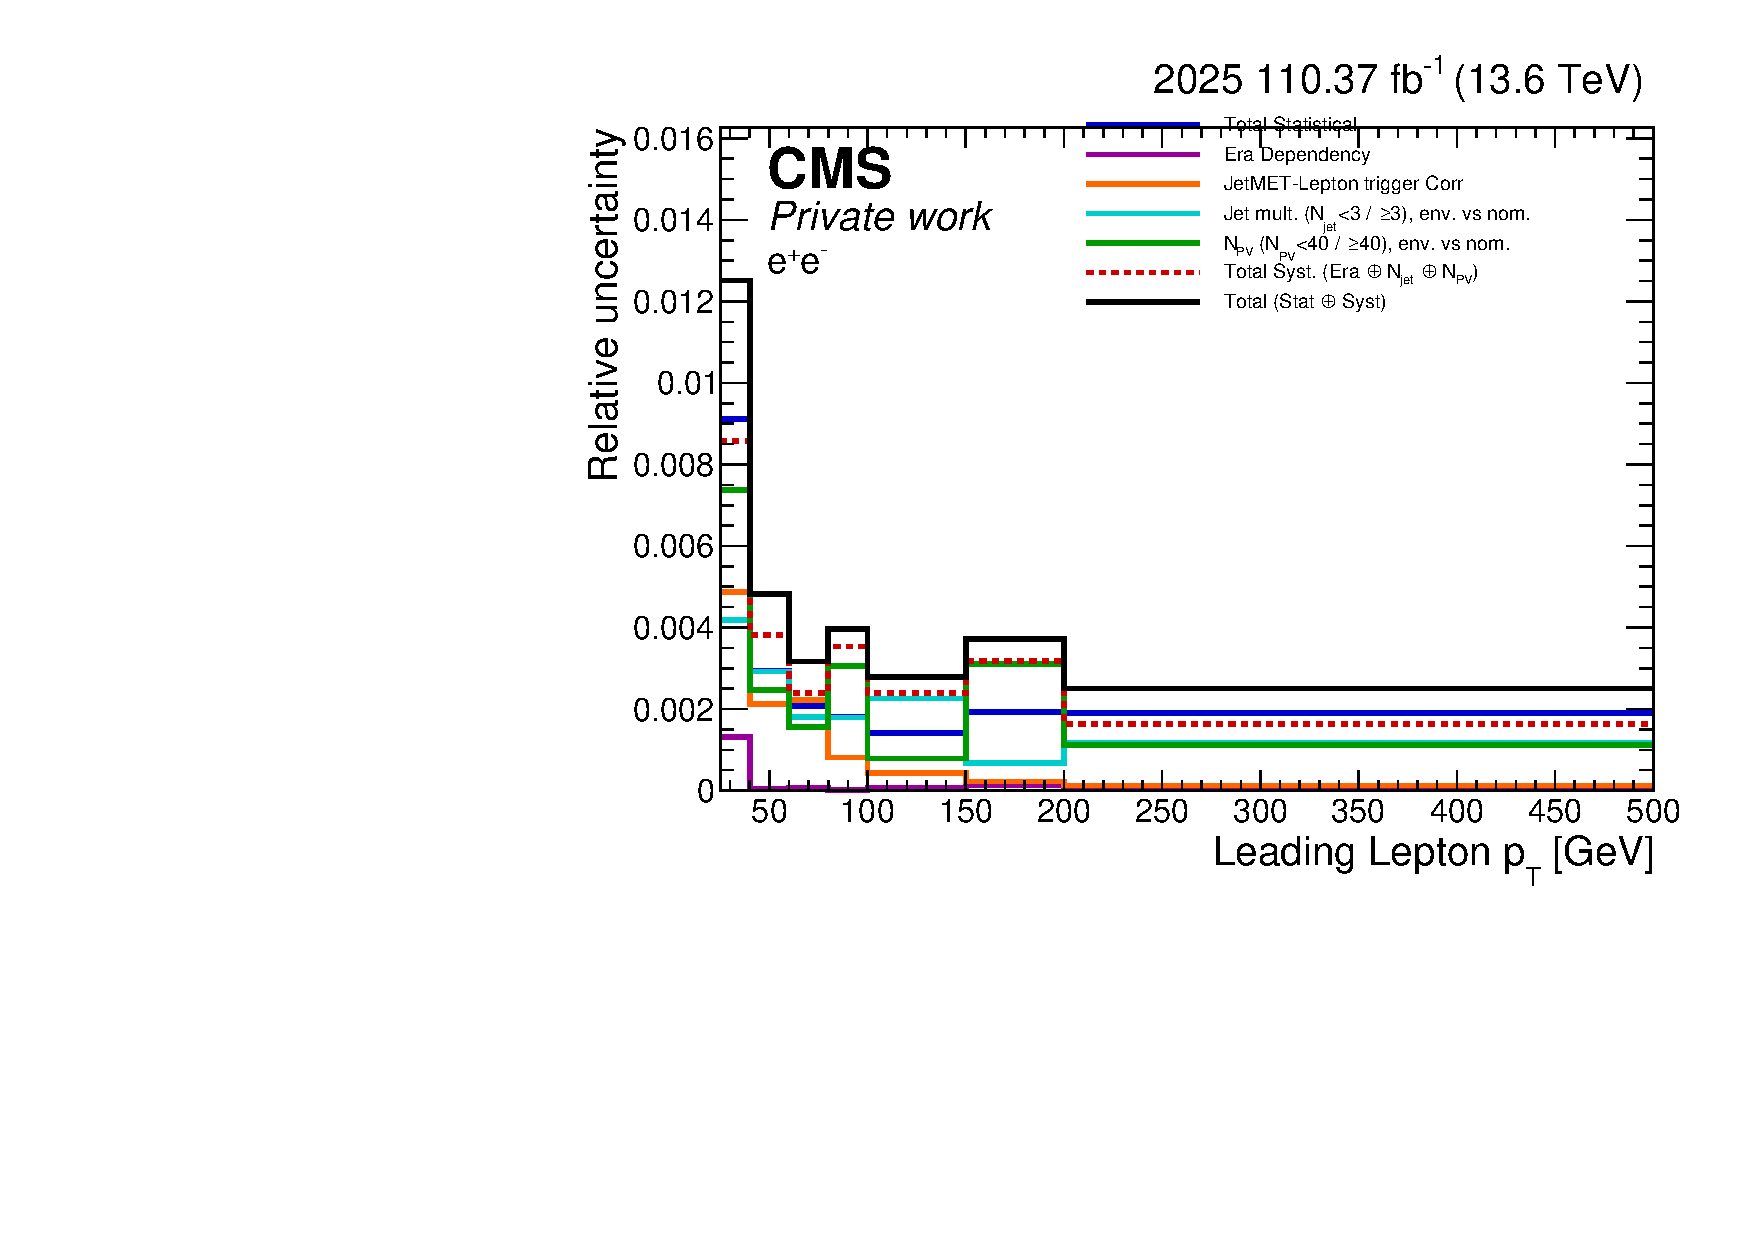
\includegraphics[width=0.48\linewidth]{figures/2025/ElEl/Relative_Uncertainty_Breakdown/Breakdown_Lep1pt.pdf}
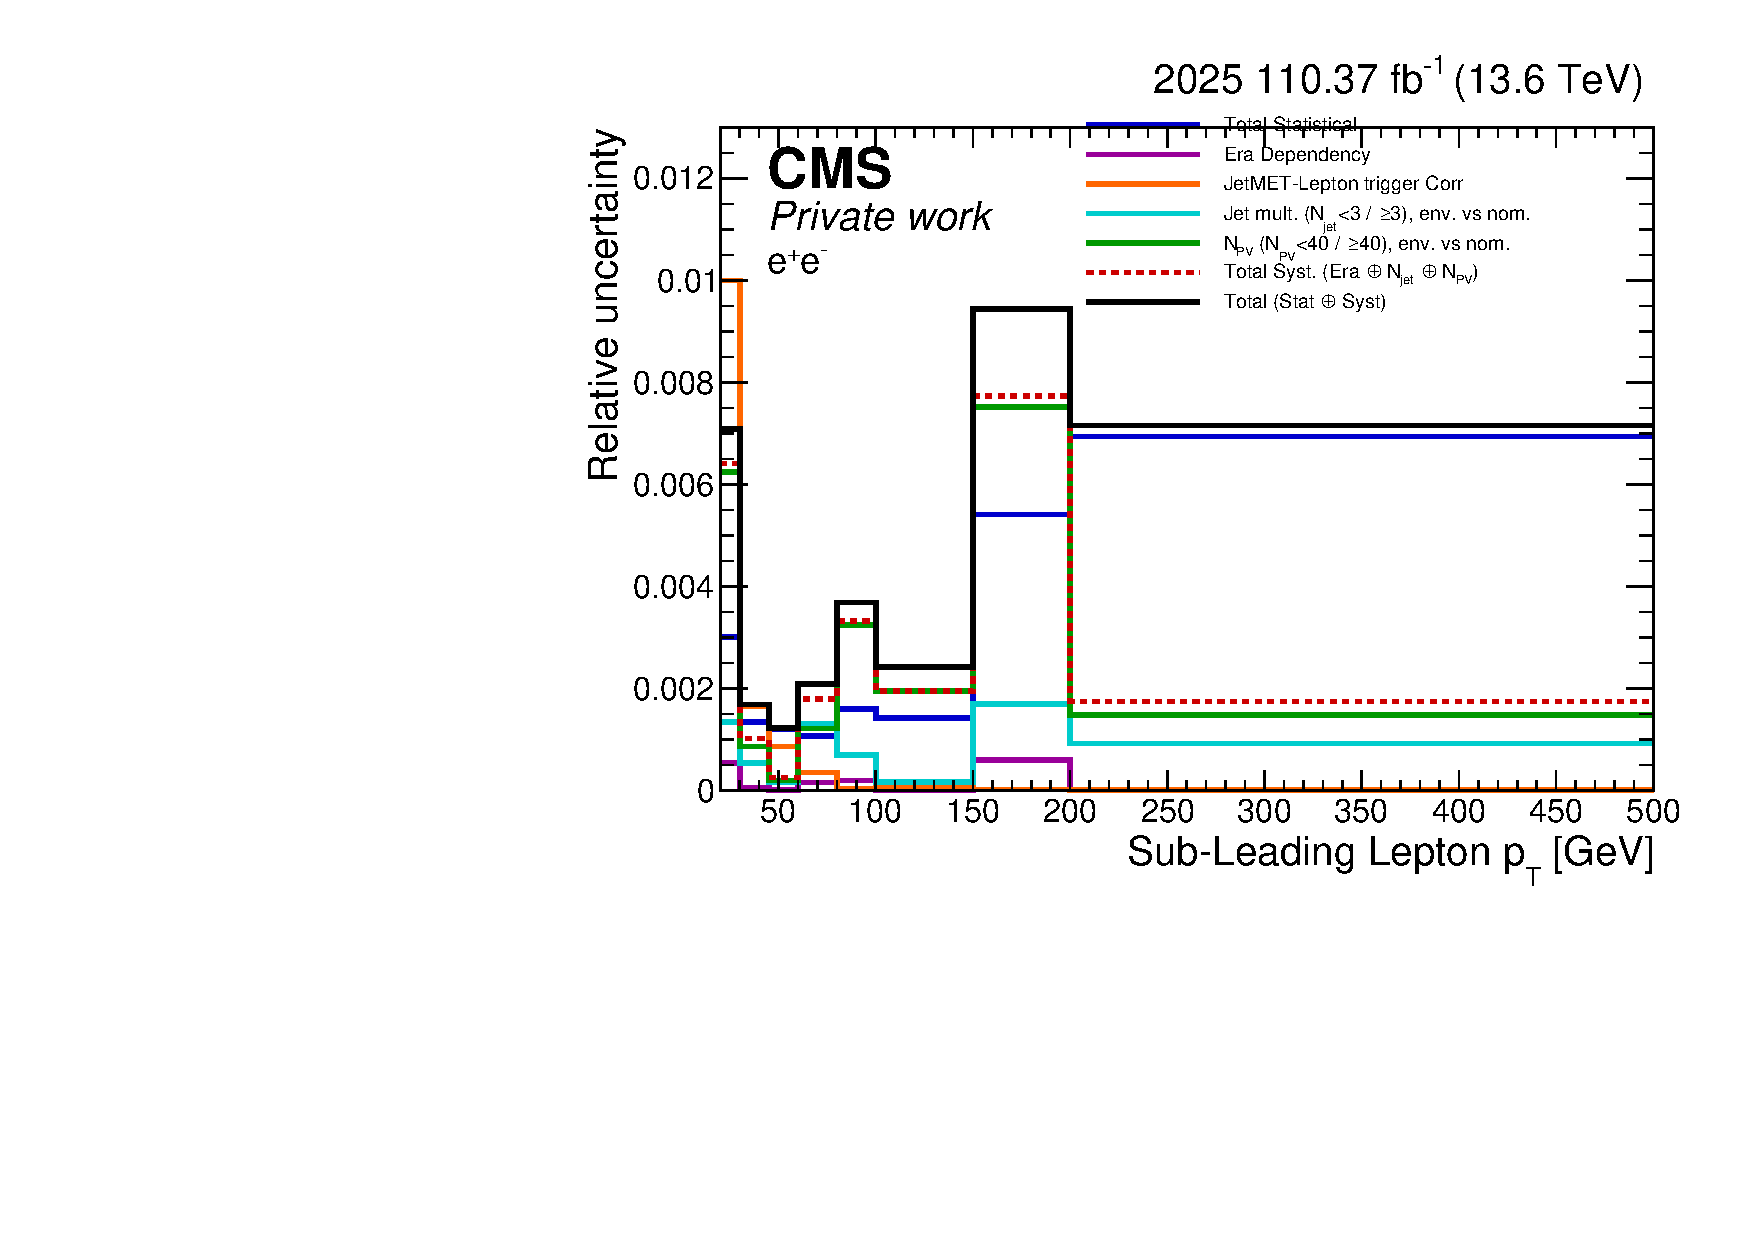
\includegraphics[width=0.48\linewidth]{figures/2025/ElEl/Relative_Uncertainty_Breakdown/Breakdown_Lep2pt.pdf}
\caption{2025: Relative uncertainty breakdown in the $ee$ channel versus leading and subleading lepton transverse momentum. The displayed total-systematic legend lists era, jet, and vertex components; the separately drawn correlation component is not listed in that sum.}\label{fig:unc-ElEl-2025}
\end{figure}
\begin{figure}[htbp]\centering
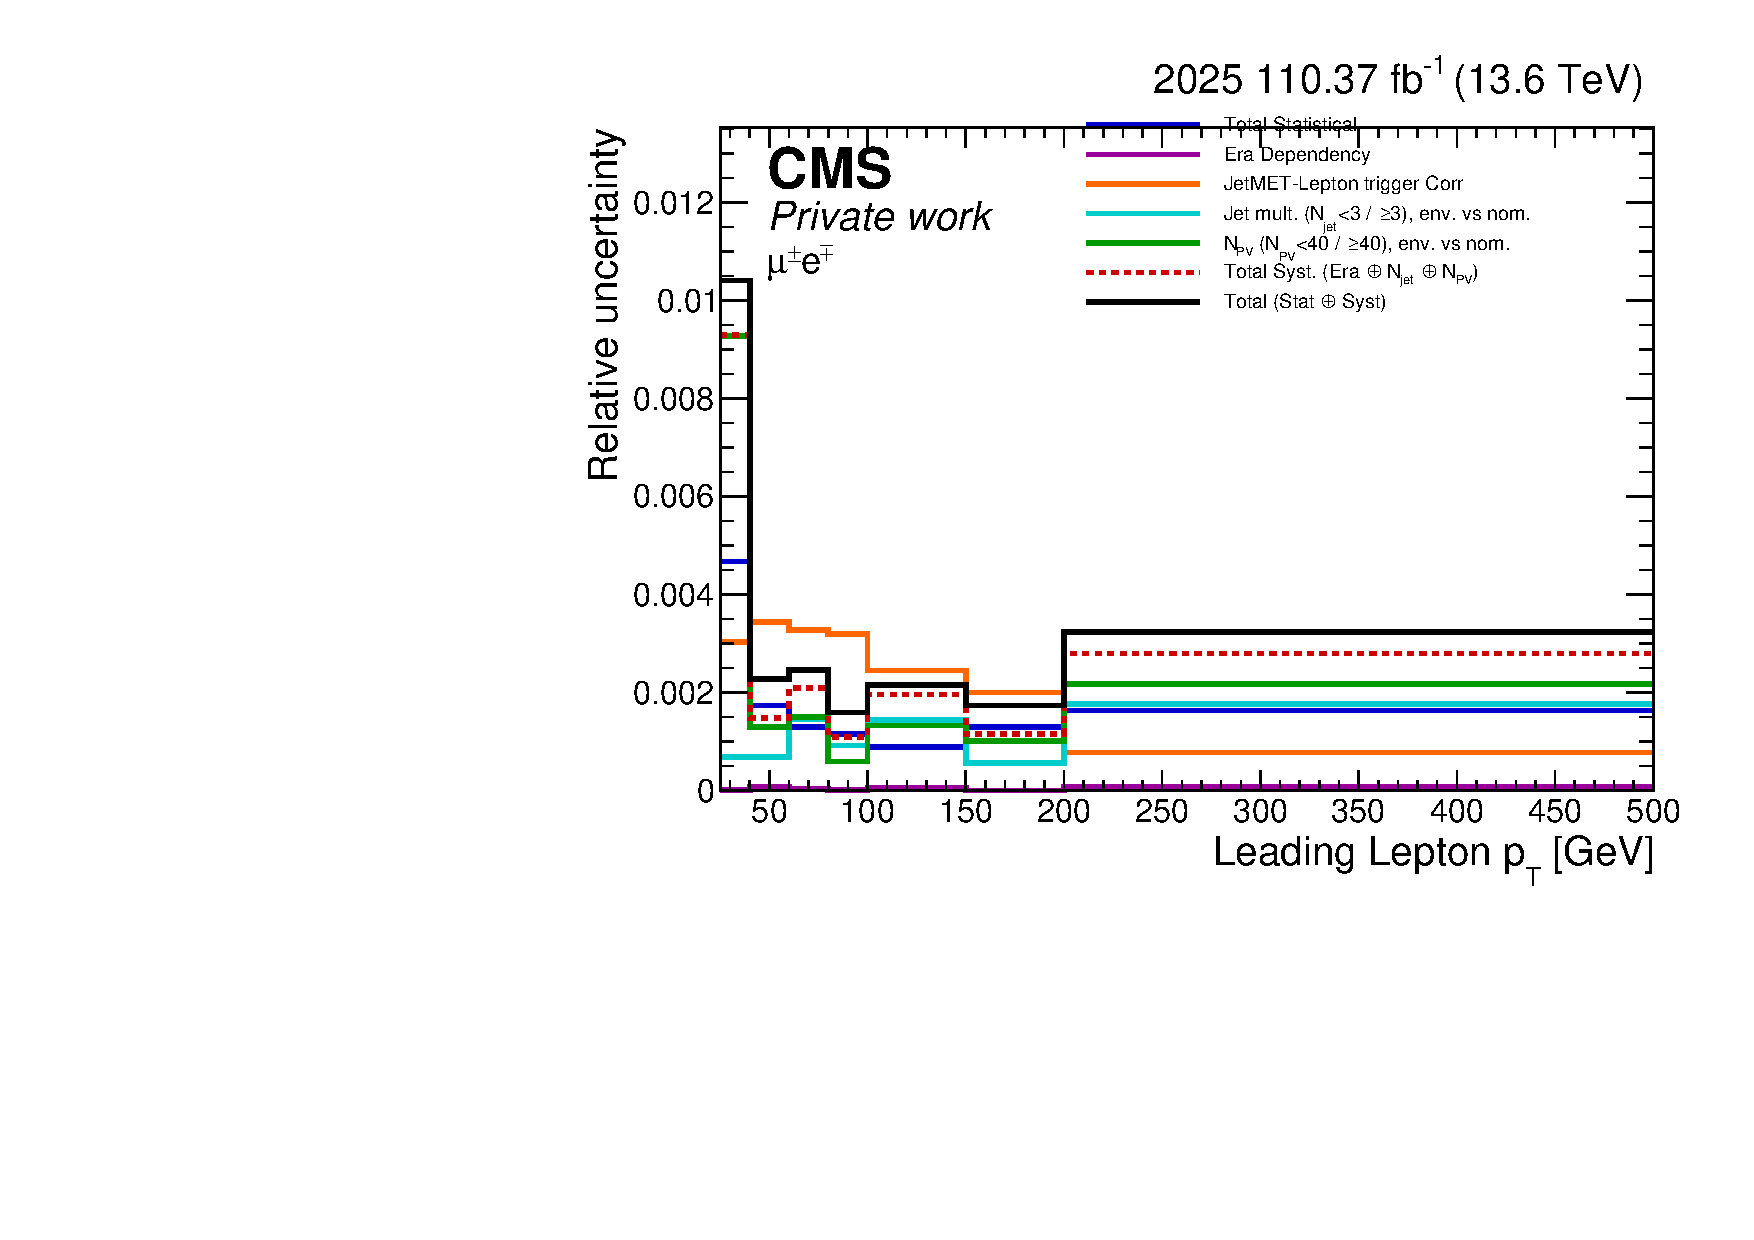
\includegraphics[width=0.48\linewidth]{figures/2025/MuEl/Relative_Uncertainty_Breakdown/Breakdown_Lep1pt.pdf}
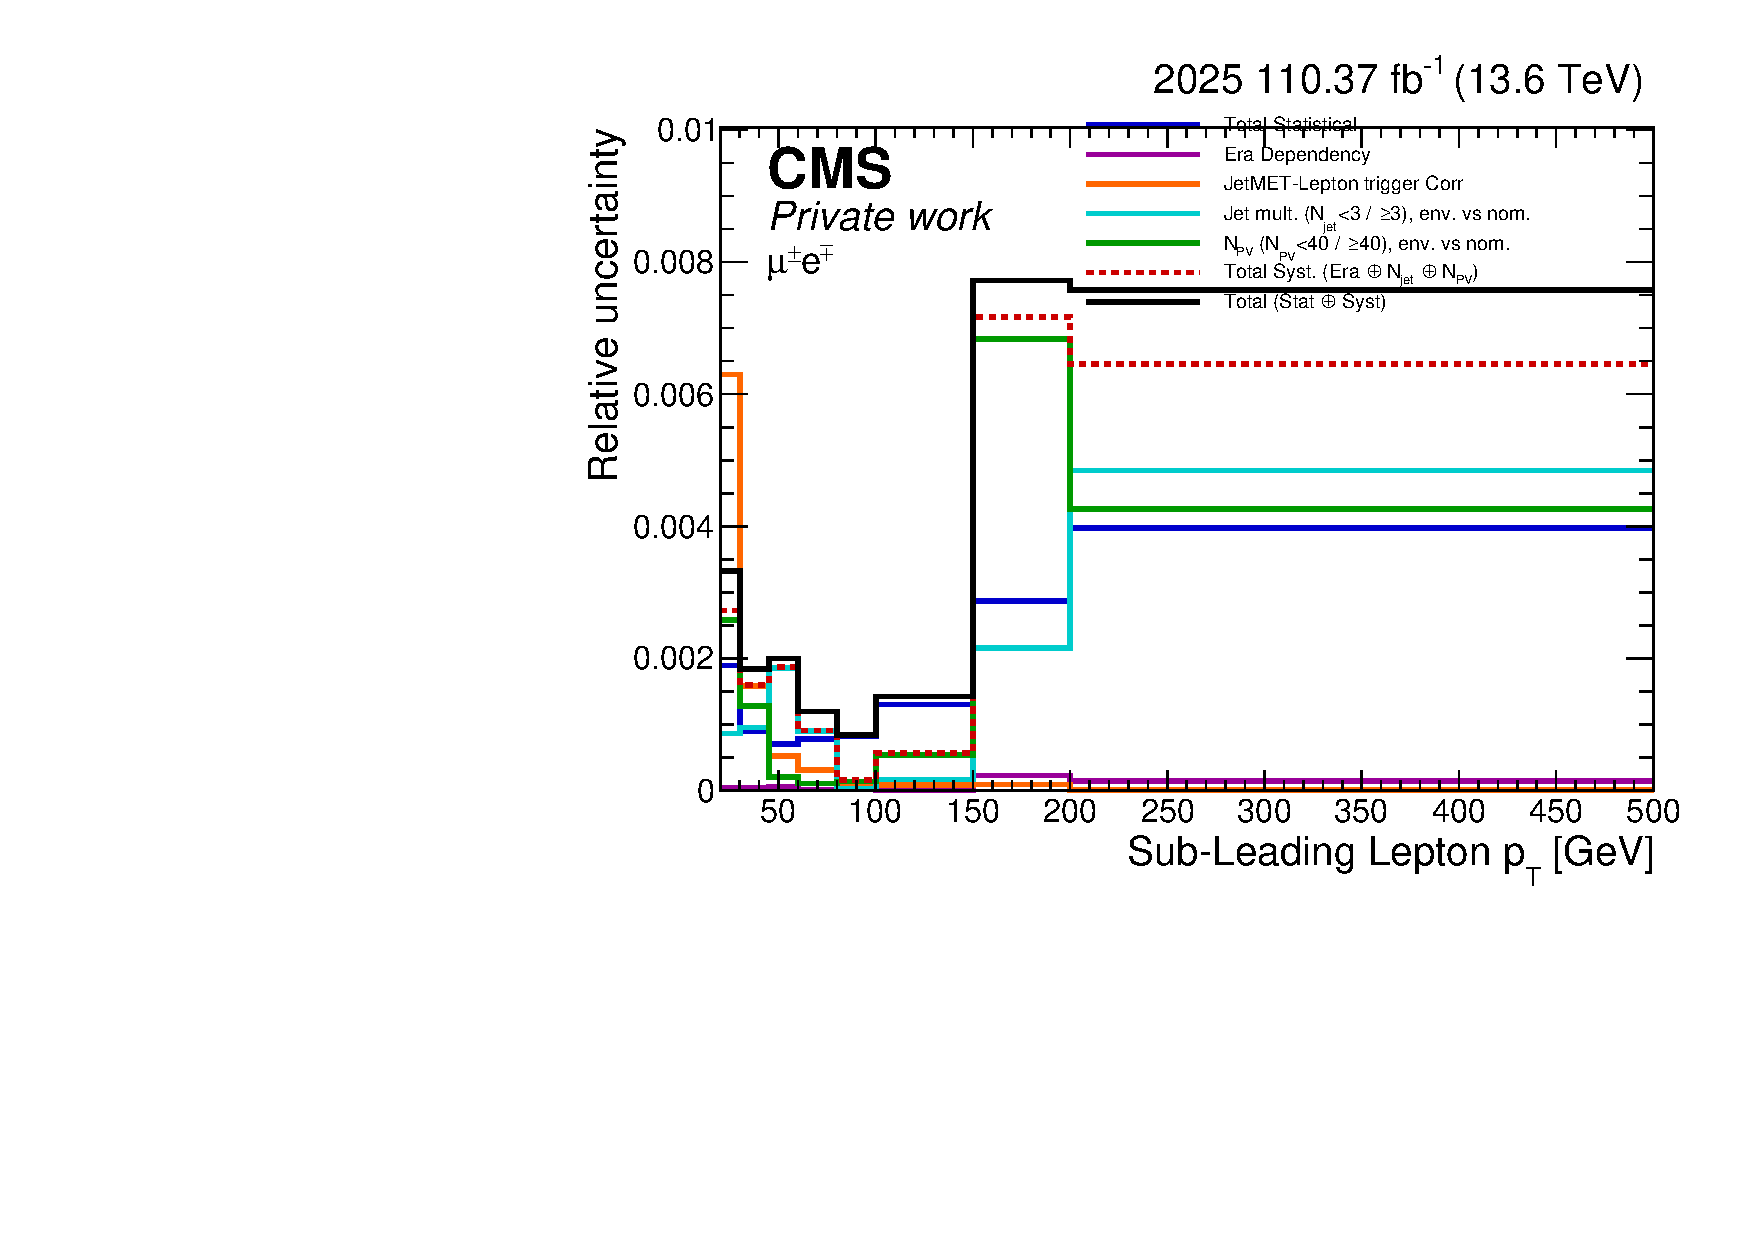
\includegraphics[width=0.48\linewidth]{figures/2025/MuEl/Relative_Uncertainty_Breakdown/Breakdown_Lep2pt.pdf}
\caption{2025: Relative uncertainty breakdown in the $e\mu$ channel versus leading and subleading lepton transverse momentum. The displayed total-systematic legend lists era, jet, and vertex components; the separately drawn correlation component is not listed in that sum.}\label{fig:unc-MuEl-2025}
\end{figure}
\begin{figure}[htbp]\centering
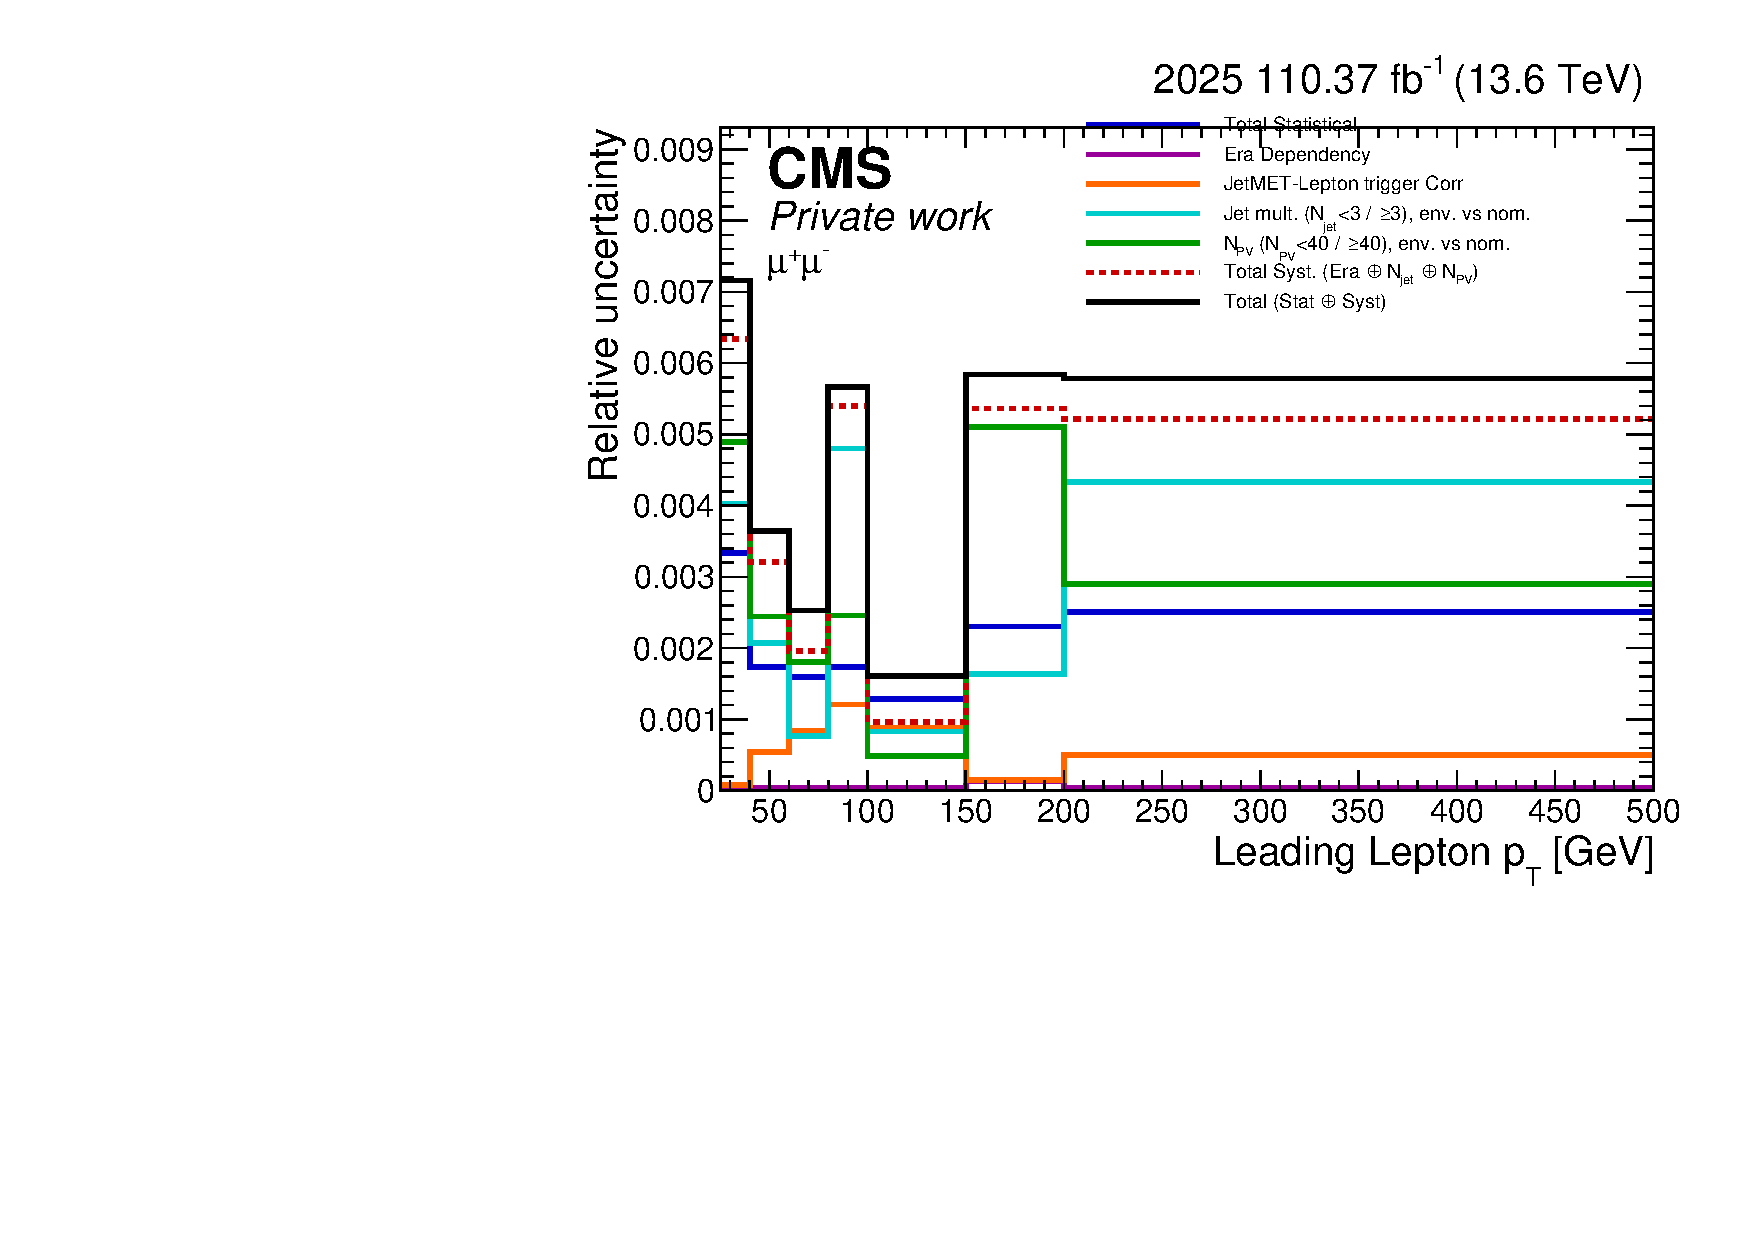
\includegraphics[width=0.48\linewidth]{figures/2025/MuMu/Relative_Uncertainty_Breakdown/Breakdown_Lep1pt.pdf}
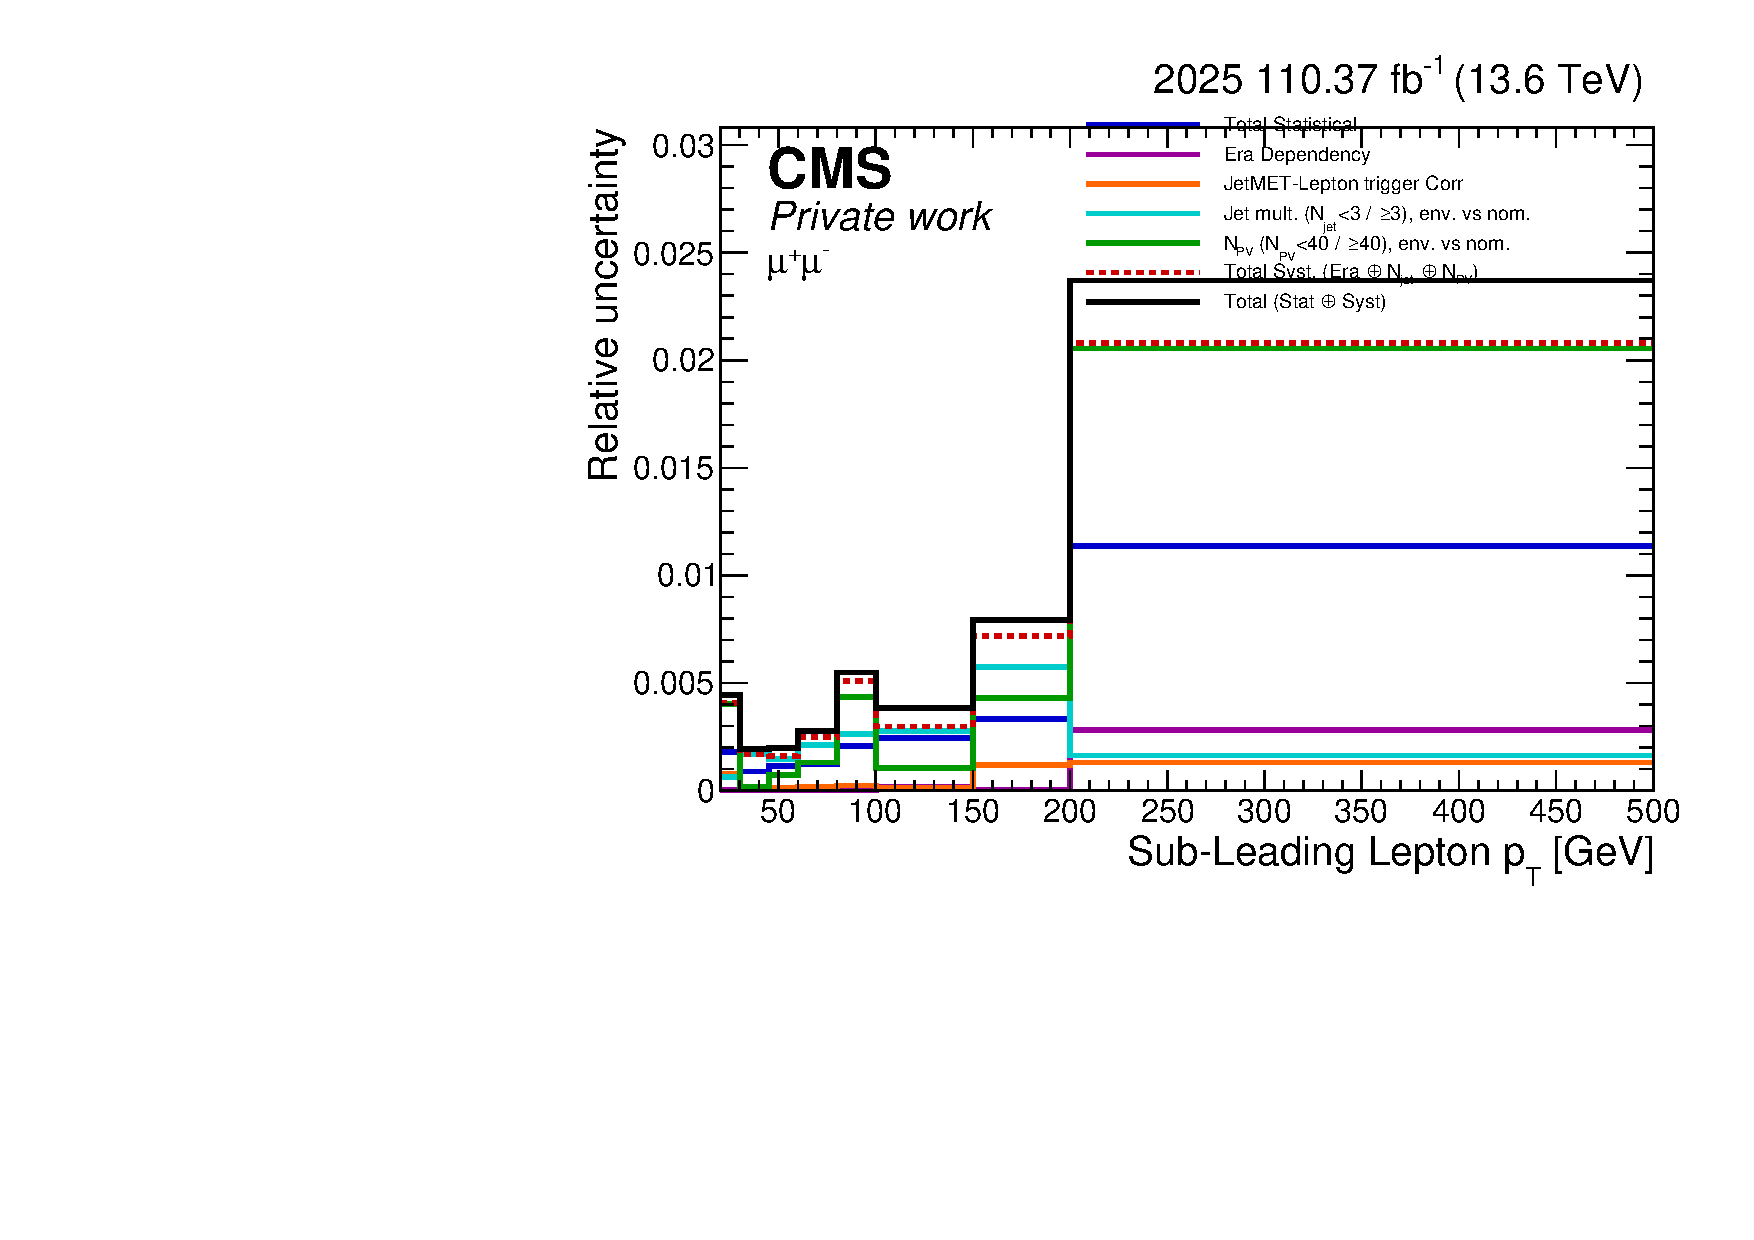
\includegraphics[width=0.48\linewidth]{figures/2025/MuMu/Relative_Uncertainty_Breakdown/Breakdown_Lep2pt.pdf}
\caption{2025: Relative uncertainty breakdown in the $\mu\mu$ channel versus leading and subleading lepton transverse momentum. The displayed total-systematic legend lists era, jet, and vertex components; the separately drawn correlation component is not listed in that sum.}\label{fig:unc-MuMu-2025}
\end{figure}

\section{Results}\label{sec:results}
This section will display the \emph{complete} finalized results, not a selected subset: every approved measurement period and each of $ee$, $e\mu$ and $\mu\mu$. Section~\ref{sec:method} introduces the method using representative one-dimensional distributions; all final central values and corresponding statistical, systematic and total uncertainties belong here. Additional diagnostic distributions are in Appendix~\ref{app:diagnostics}. No measured values or maps were included in the supplied source material for the CPV selection, so the following are labelled figure slots.
\subsection{One-dimensional efficiencies and scale factors}\label{sec:oneD}
For each period and channel, show efficiencies in data and MC and their ratio versus leading and subleading lepton $p_{\mathrm T}$ and $\eta$. Display denominator yields, binning, uncertainty bars and reference-trigger choice. \insertitem{Full one-dimensional figure set and captions for each period $\times$ channel.}
\subsection{Two-dimensional central scale factors and uncertainties}\label{sec:twoD}
For each period, group the $ee$, $e\mu$ and $\mu\mu$ central SF maps with the matching statistical, systematic and total uncertainty maps; mark invalid bins and the exact lookup convention. If a large number of finely divided periods makes the document unwieldy, use a per-period figure followed immediately by its uncertainty figures, preserving the full set in this section rather than moving final maps to the appendix.
\begin{figure}[htbp]\centering\plotplaceholder{All final $ee$, $e\mu$, $\mu\mu$ SF($p_{\rm T}^{\ell_1},p_{\rm T}^{\ell_2}$) maps, repeated for each approved period.}\caption{Final two-dimensional central trigger scale factors. Replace this slot with the complete set of measured maps and bin definitions.}\label{fig:final-sf}\end{figure}
\begin{figure}[htbp]\centering\plotplaceholder{Matching per-bin statistical, systematic and total uncertainty maps for every channel and period.}\caption{Final two-dimensional trigger scale-factor uncertainties matching Fig.~\ref{fig:final-sf}. Replace this slot with the complete set of measured maps.}\label{fig:final-unc}\end{figure}
\insertitem{Optional machine-readable correction file name, version, validity intervals, bin edges and units.}

\section{Validation and remaining checks}\label{sec:closure}
The supplied result set contains one-dimensional dependence studies and uncertainty variations, but no identified independent before/after-SF closure comparison. The one-dimensional efficiency ratios used to construct the correction are not independent closure tests. Application closure is therefore not claimed in this draft.
An appropriate next test applies the fixed 2D correction in a statistically independent subset or justified control region and compares data with simulated selected yields before and after correction. Lepton momentum and pseudorapidity, missing momentum, and jet and vertex multiplicities should be checked with a stated normalization and background treatment. Residual one-dimensional trends may indicate missing dependence but cannot by themselves distinguish a trigger bias from composition, calibration, or other modelling effects.
\todo{Provide an independent validation region, before/after plots, uncertainty propagation, and a quantitative comparison.}

\section{Summary}
This note documents the Run 3 dilepton trigger measurement. The current draft includes 2024 and 2025 results; other Run 3 years will be included in subsequent updates. The supplied 2024 and 2025 results provide dilepton trigger efficiency comparisons and two-dimensional data-to-simulation scale-factor maps for $ee$, $e\mu$, and $\mu\mu$. The one-dimensional figure labels quote $109.82~\mathrm{fb}^{-1}$ for 2024 and $110.37~\mathrm{fb}^{-1}$ for 2025 at 13.6 TeV. Same-flavour maps use ordered lepton momenta; the mixed-flavour map uses electron and muon momenta. Statistical, topology, pileup, era, and correlation studies accompany the measurement. Final release requires confirmation of the production selections and input samples, resolution of the correlation-error combination, validation of the ROOT lookup semantics, and an independent application cross-check.


\clearpage
\newpage
\bibliography{auto_generated}

\clearpage
\appendix
\section{2024: additional kinematic dependence}\label{app:diagnostics}
These distributions extend the main momentum comparisons. They use the same measurement sample and do not constitute independent closure tests.
\begin{figure}[htbp]\centering
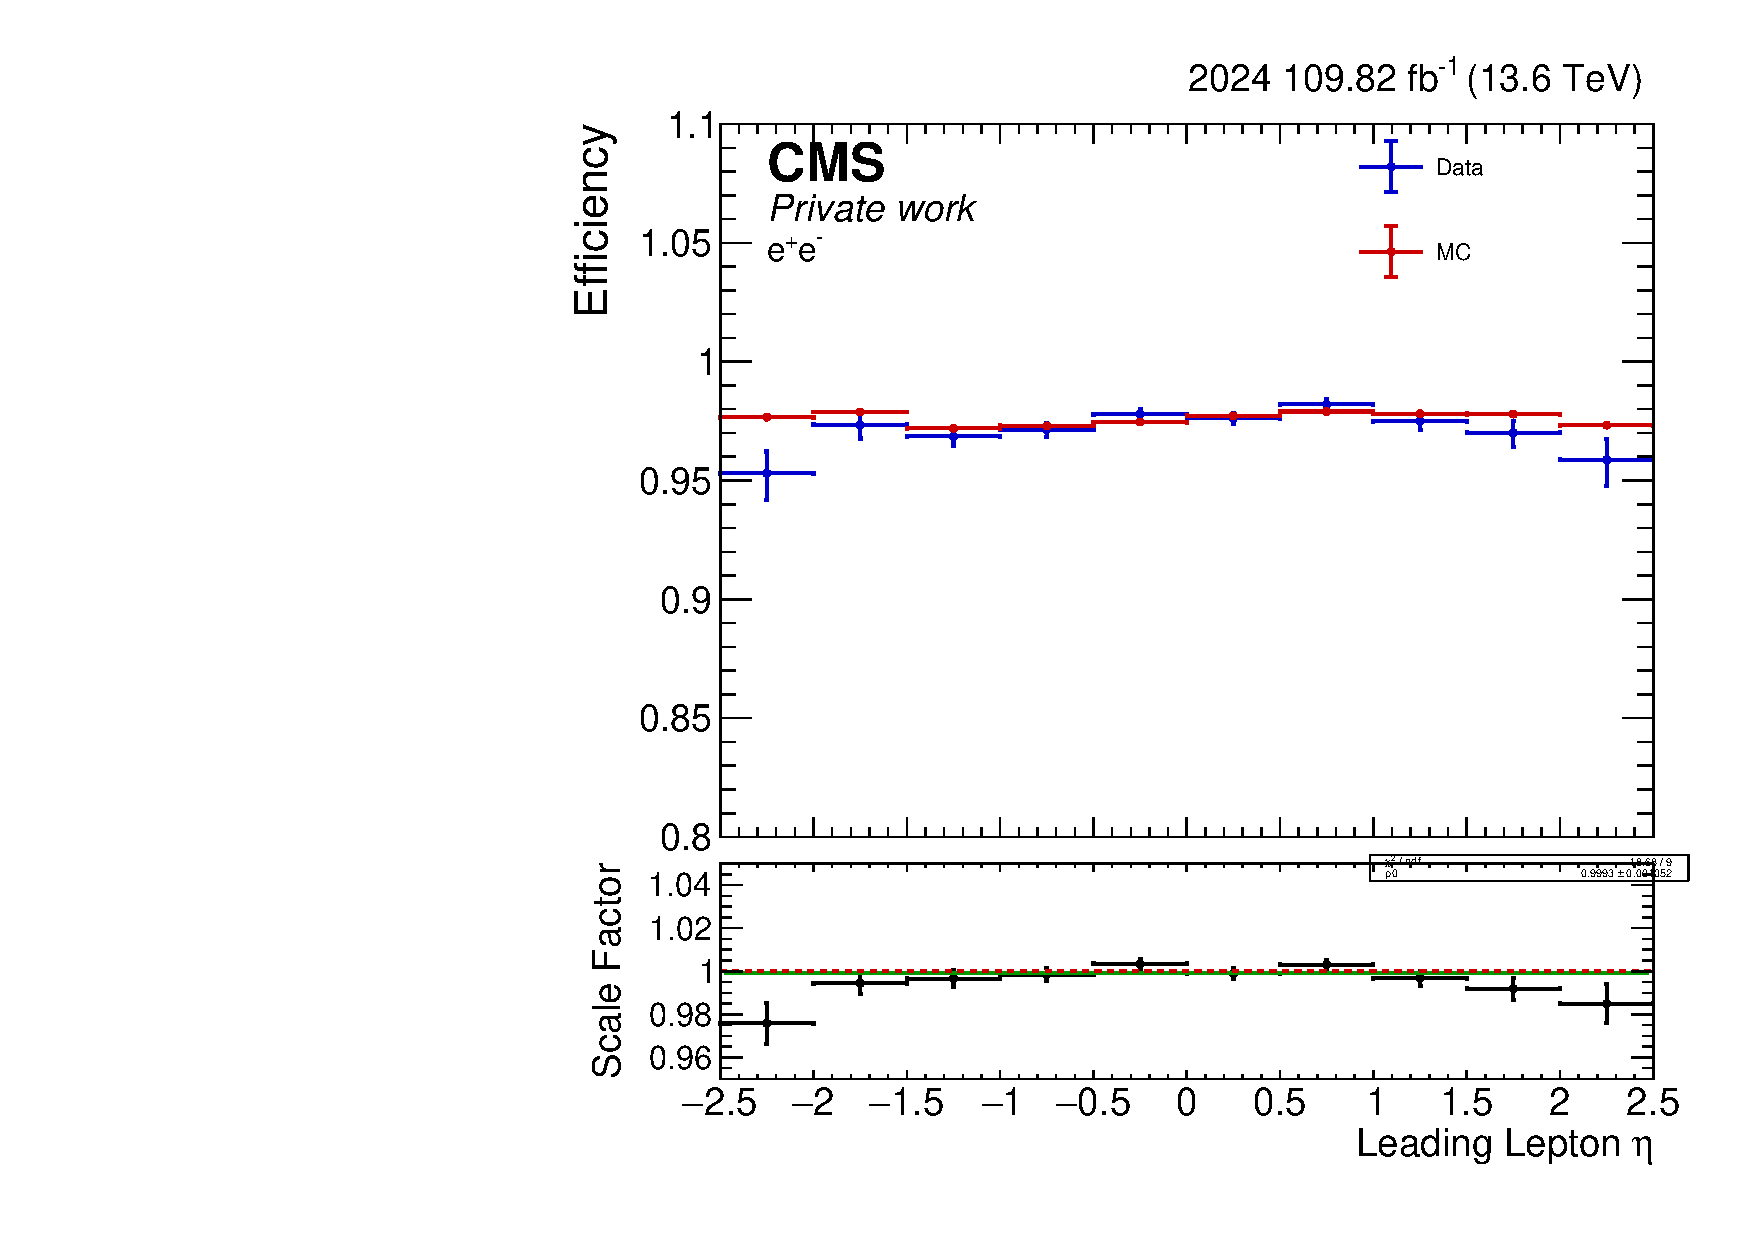
\includegraphics[width=0.48\linewidth]{figures/2024/ElEl/ScaleFactor/SF_Lep1eta.pdf}
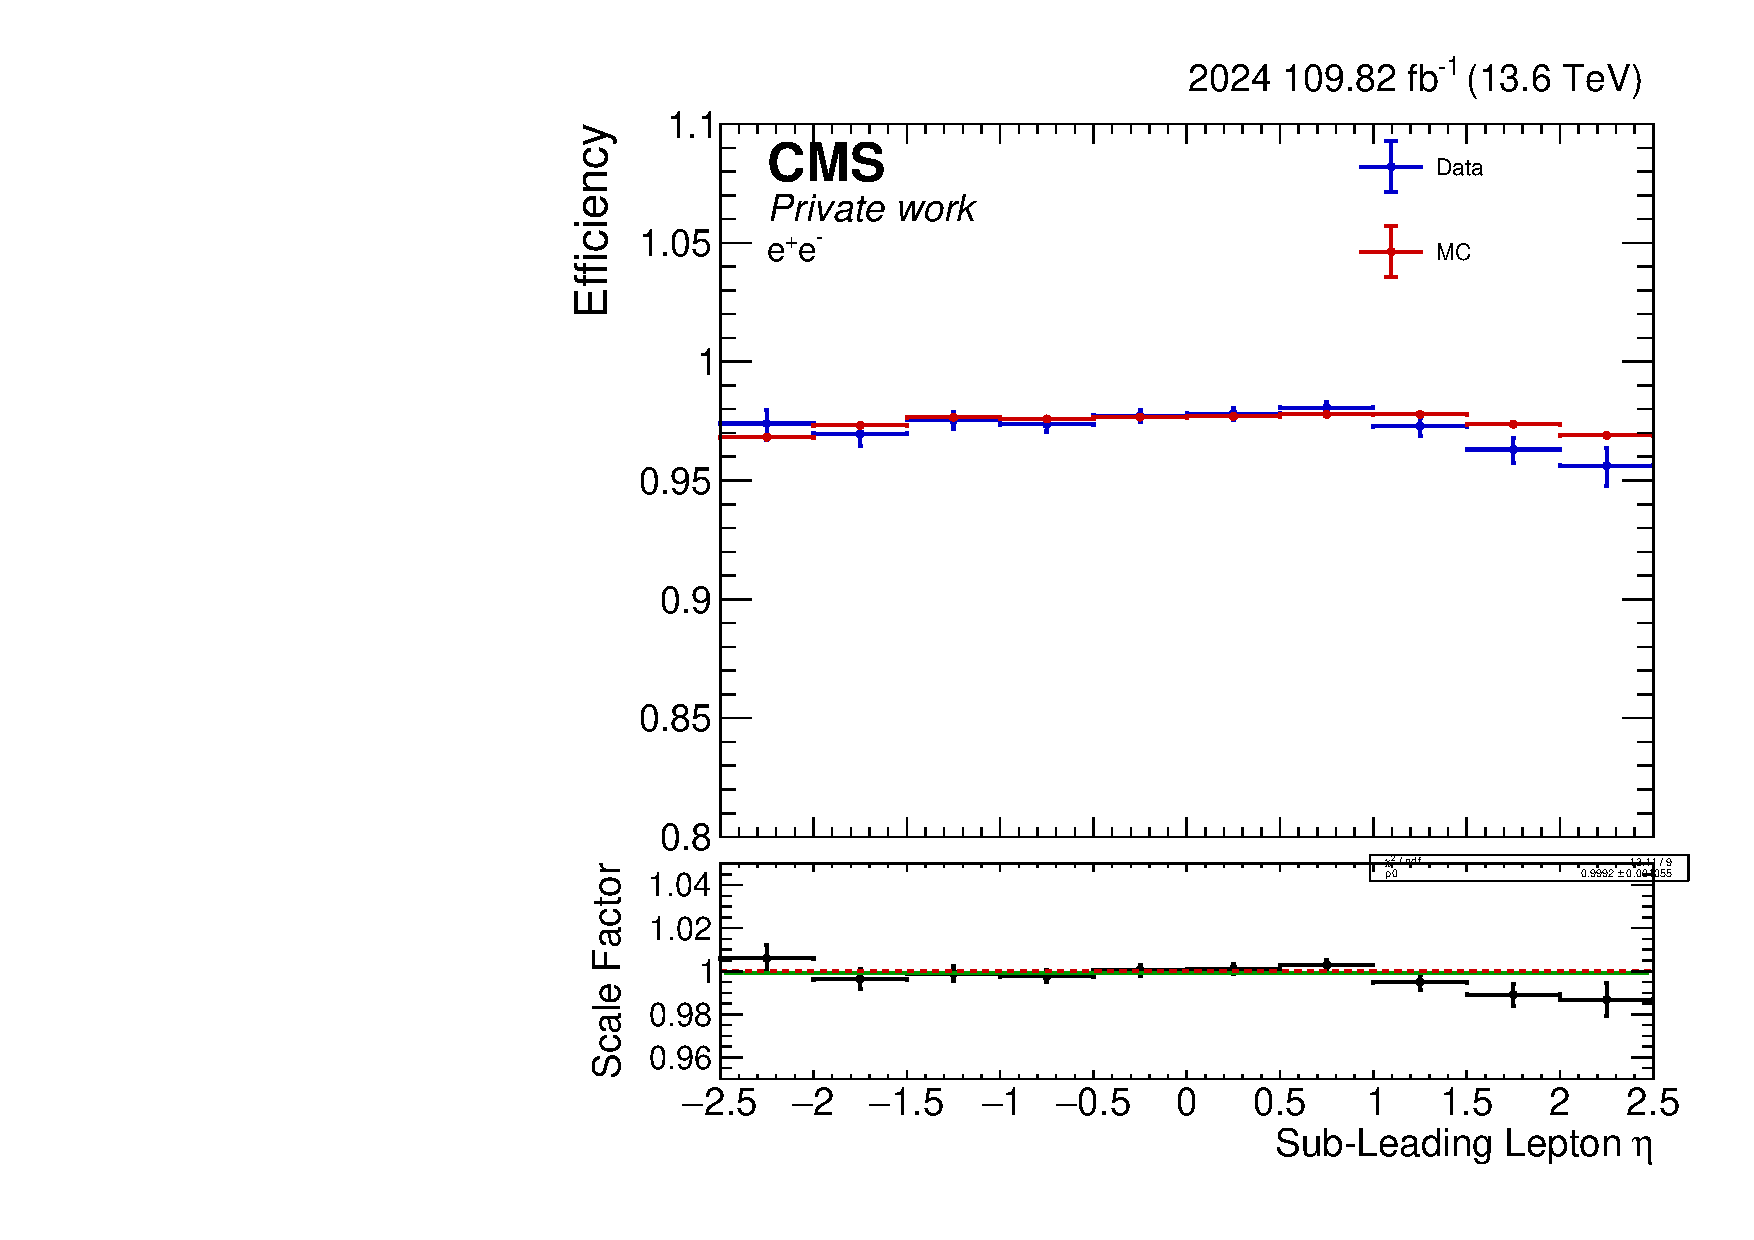
\includegraphics[width=0.48\linewidth]{figures/2024/ElEl/ScaleFactor/SF_Lep2eta.pdf}
\caption{Additional one-dimensional efficiency and SF diagnostics in the $ee$ channel. Variables and binning are shown on each axis.}\label{fig:diag-ElEl-SF_Lep1eta}
\end{figure}
\begin{figure}[htbp]\centering
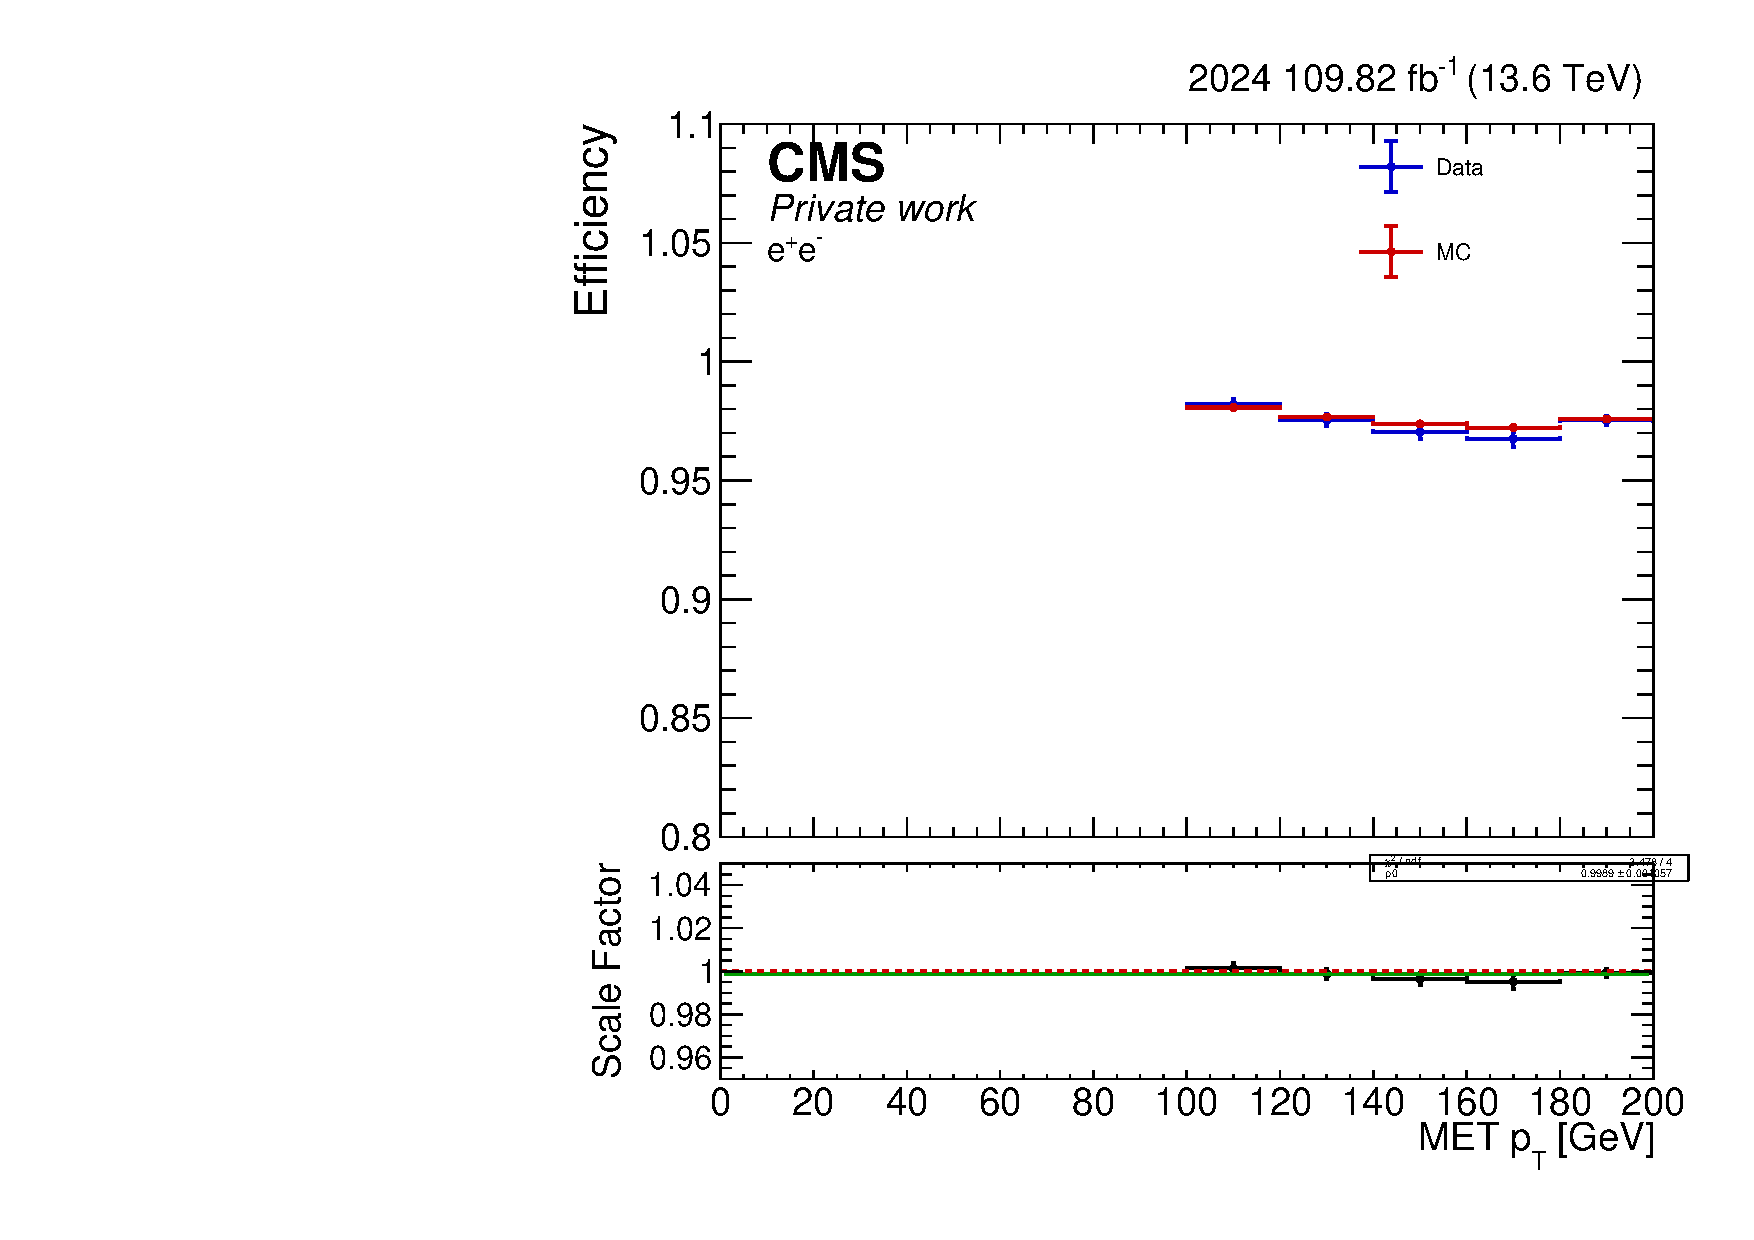
\includegraphics[width=0.48\linewidth]{figures/2024/ElEl/ScaleFactor/SF_METpt.pdf}
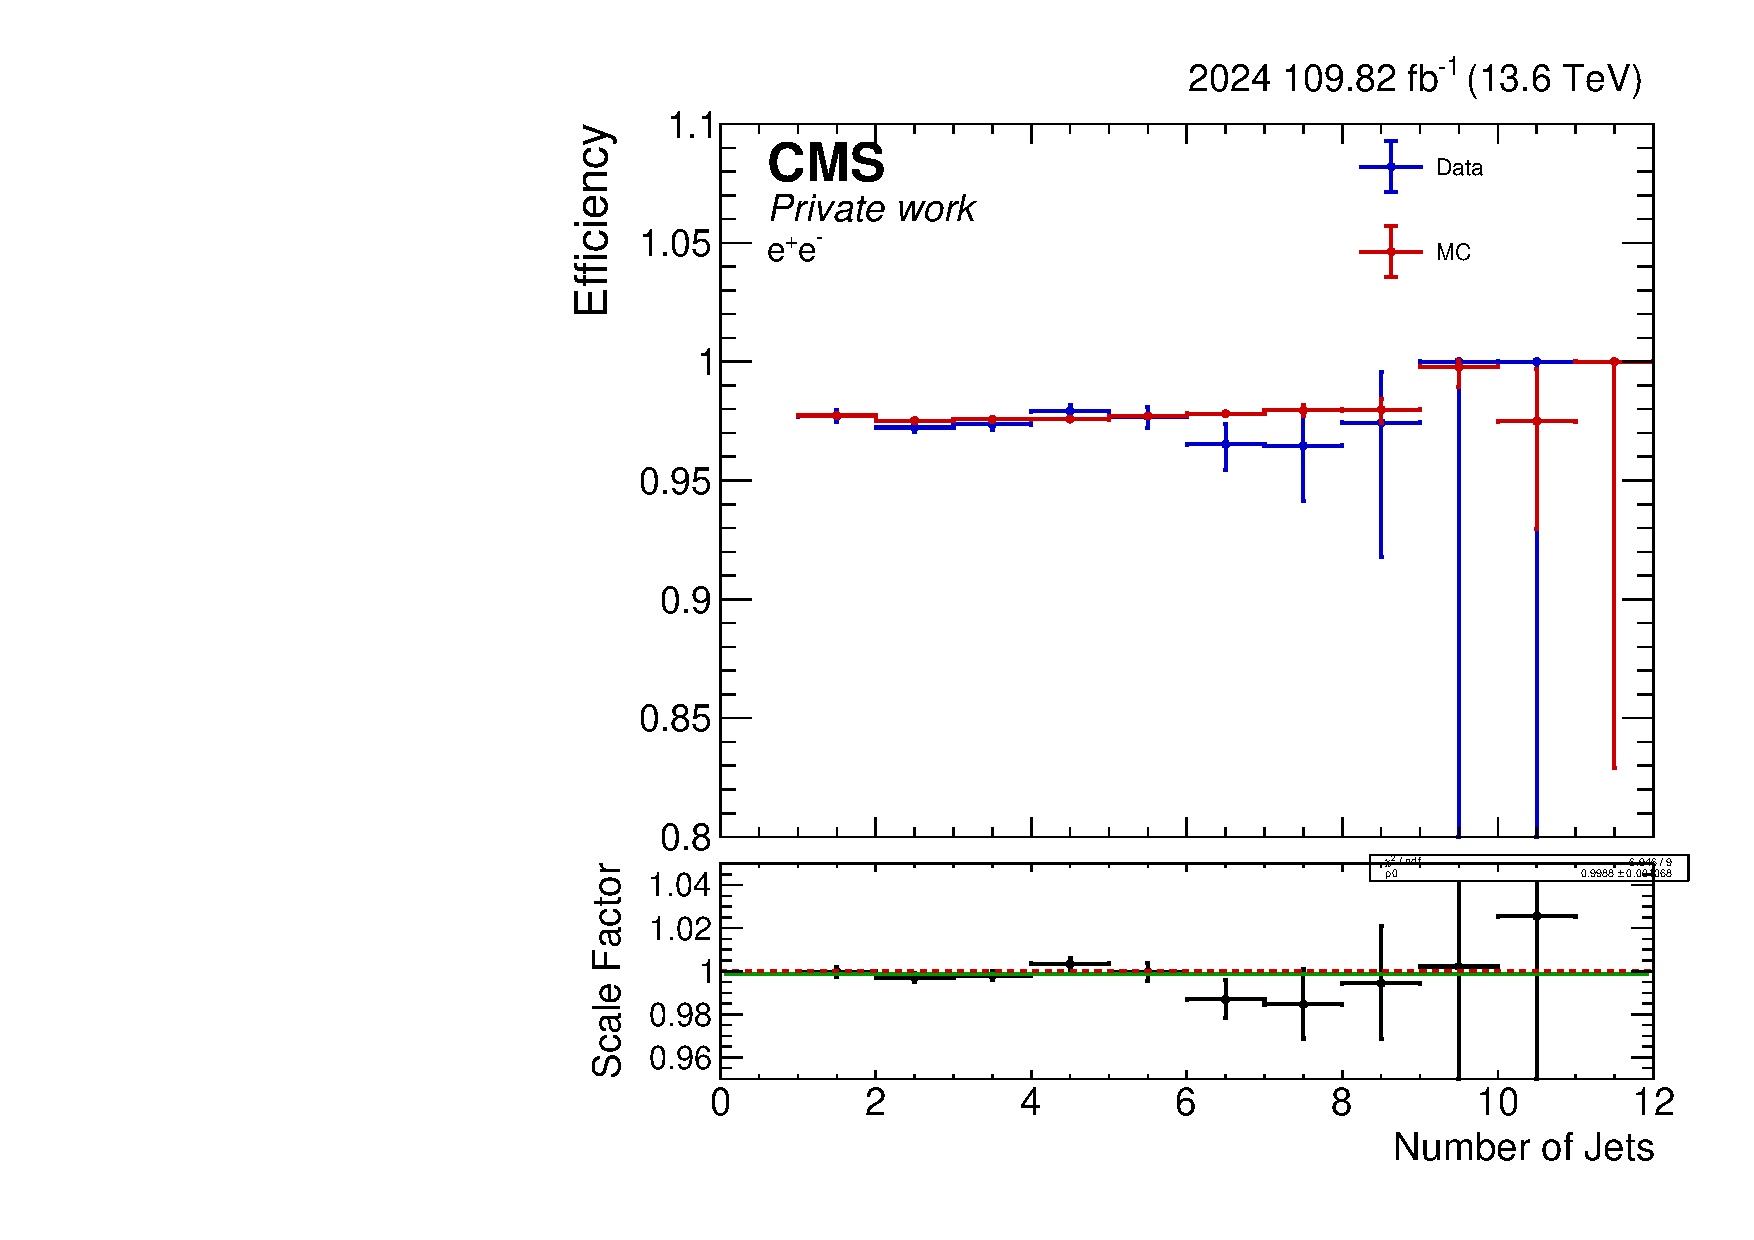
\includegraphics[width=0.48\linewidth]{figures/2024/ElEl/ScaleFactor/SF_Num_Jets.pdf}
\caption{Additional one-dimensional efficiency and SF diagnostics in the $ee$ channel. Variables and binning are shown on each axis.}\label{fig:diag-ElEl-SF_METpt}
\end{figure}
\begin{figure}[htbp]\centering
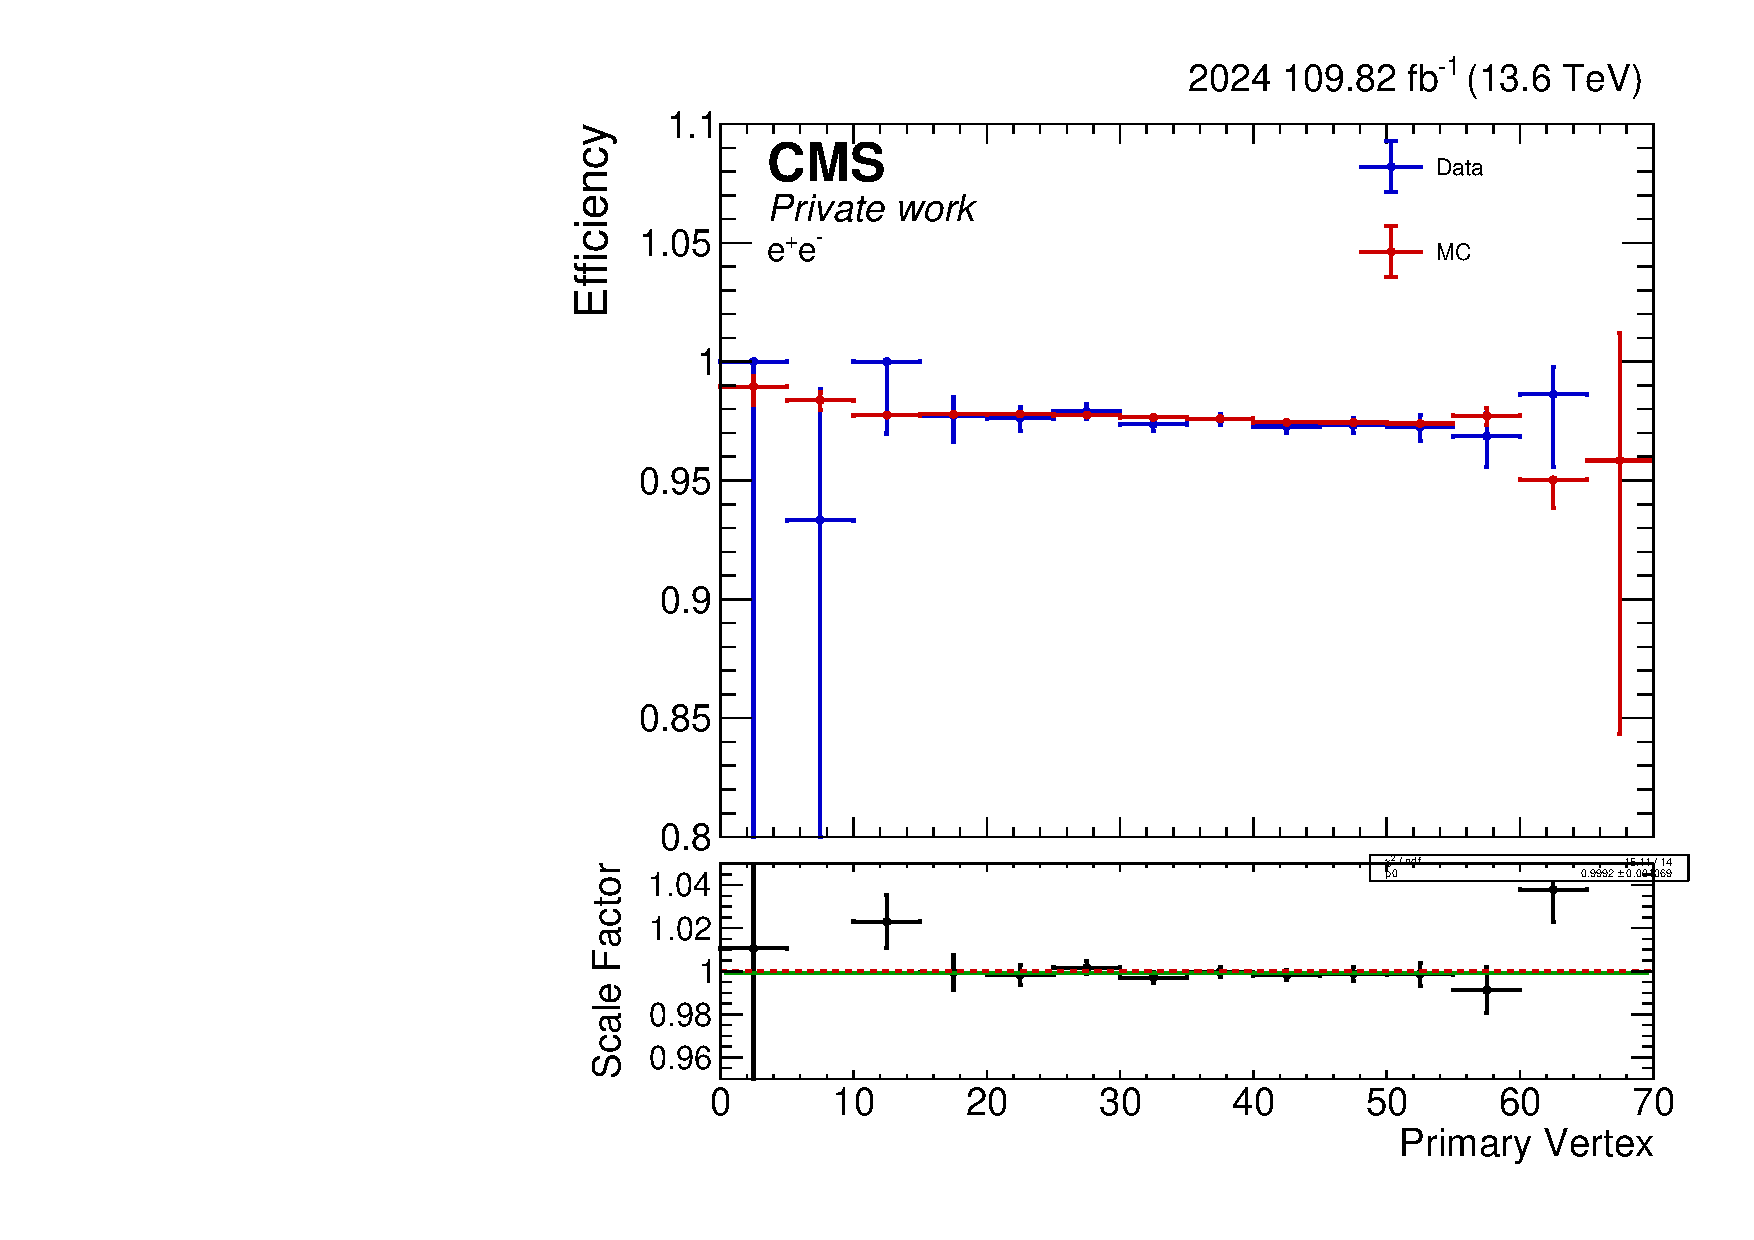
\includegraphics[width=0.48\linewidth]{figures/2024/ElEl/ScaleFactor/SF_Num_PV.pdf}
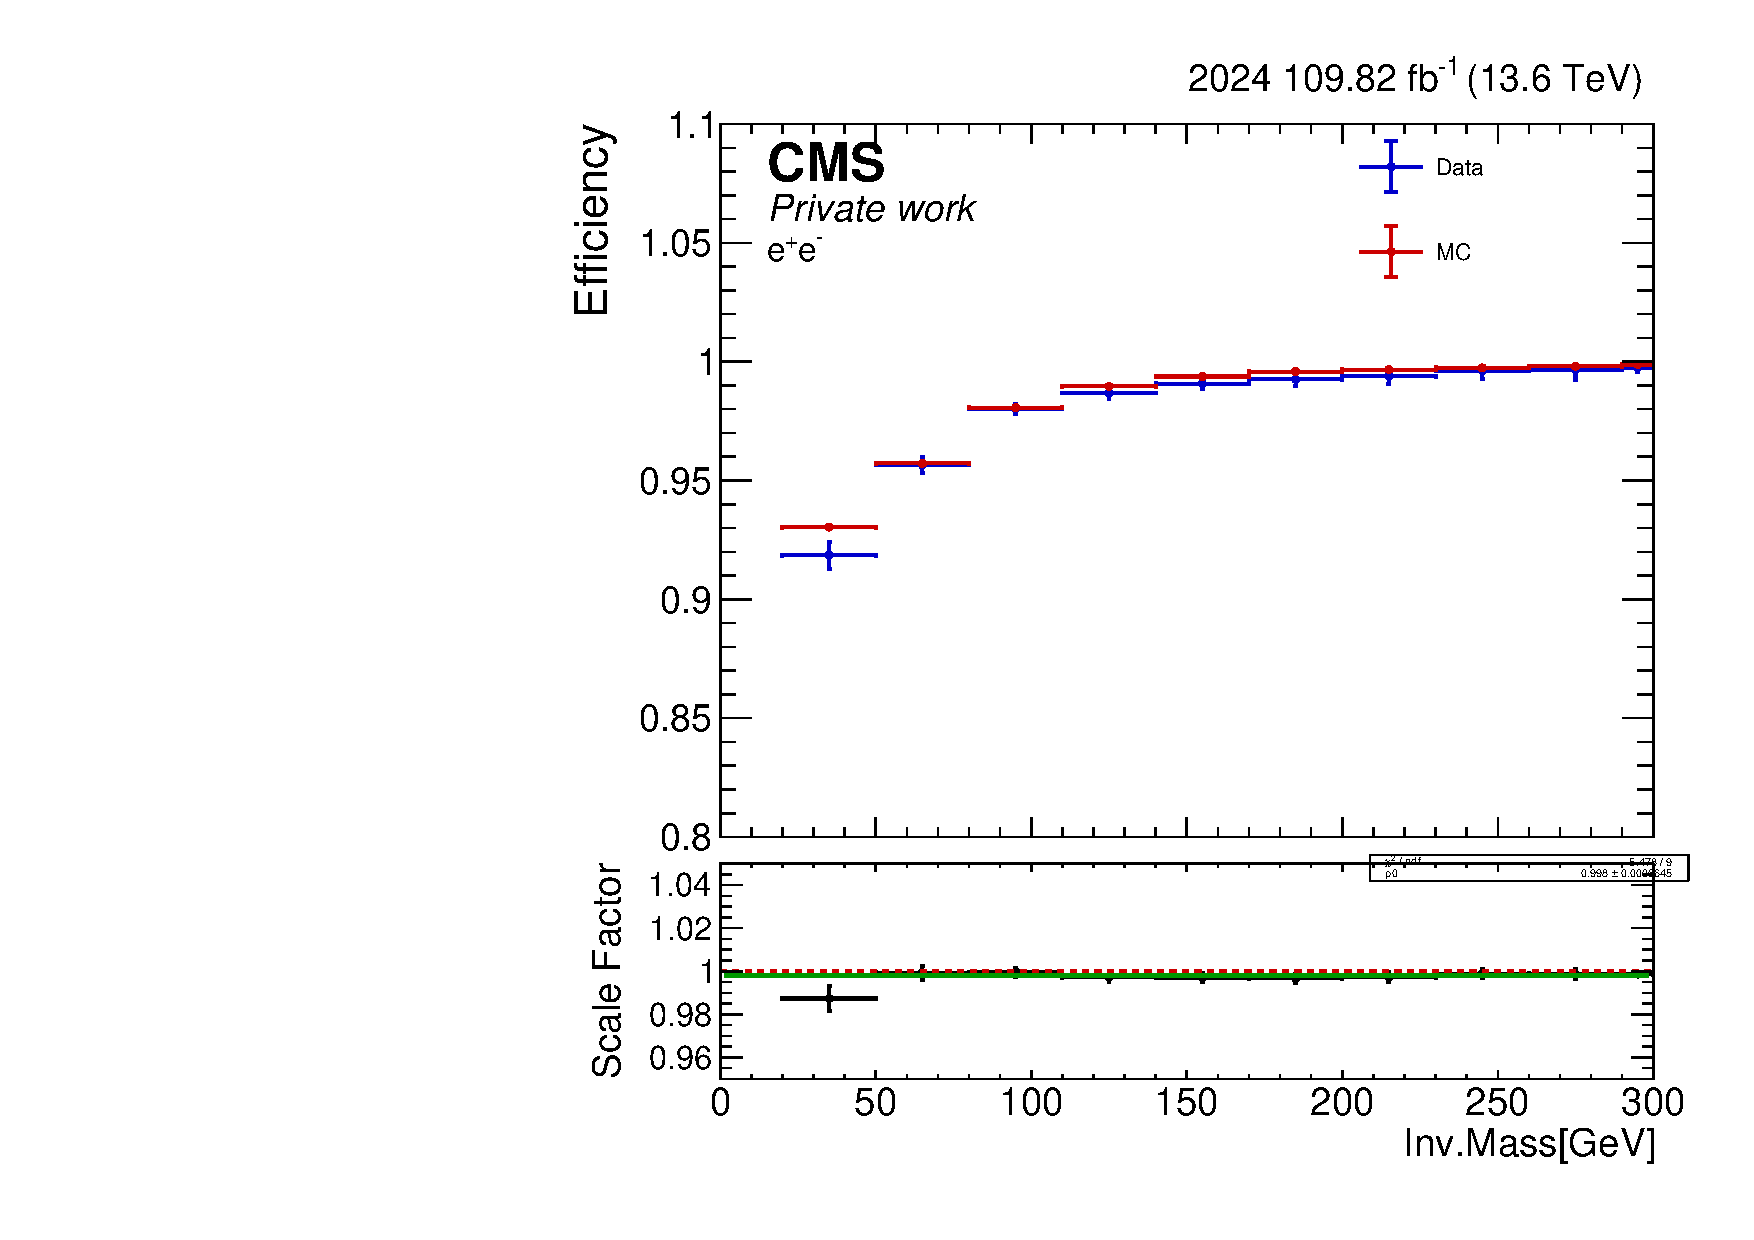
\includegraphics[width=0.48\linewidth]{figures/2024/ElEl/ScaleFactor/SF_DiLepMass.pdf}
\caption{Additional one-dimensional efficiency and SF diagnostics in the $ee$ channel. Variables and binning are shown on each axis.}\label{fig:diag-ElEl-SF_Num_PV}
\end{figure}
\begin{figure}[htbp]\centering
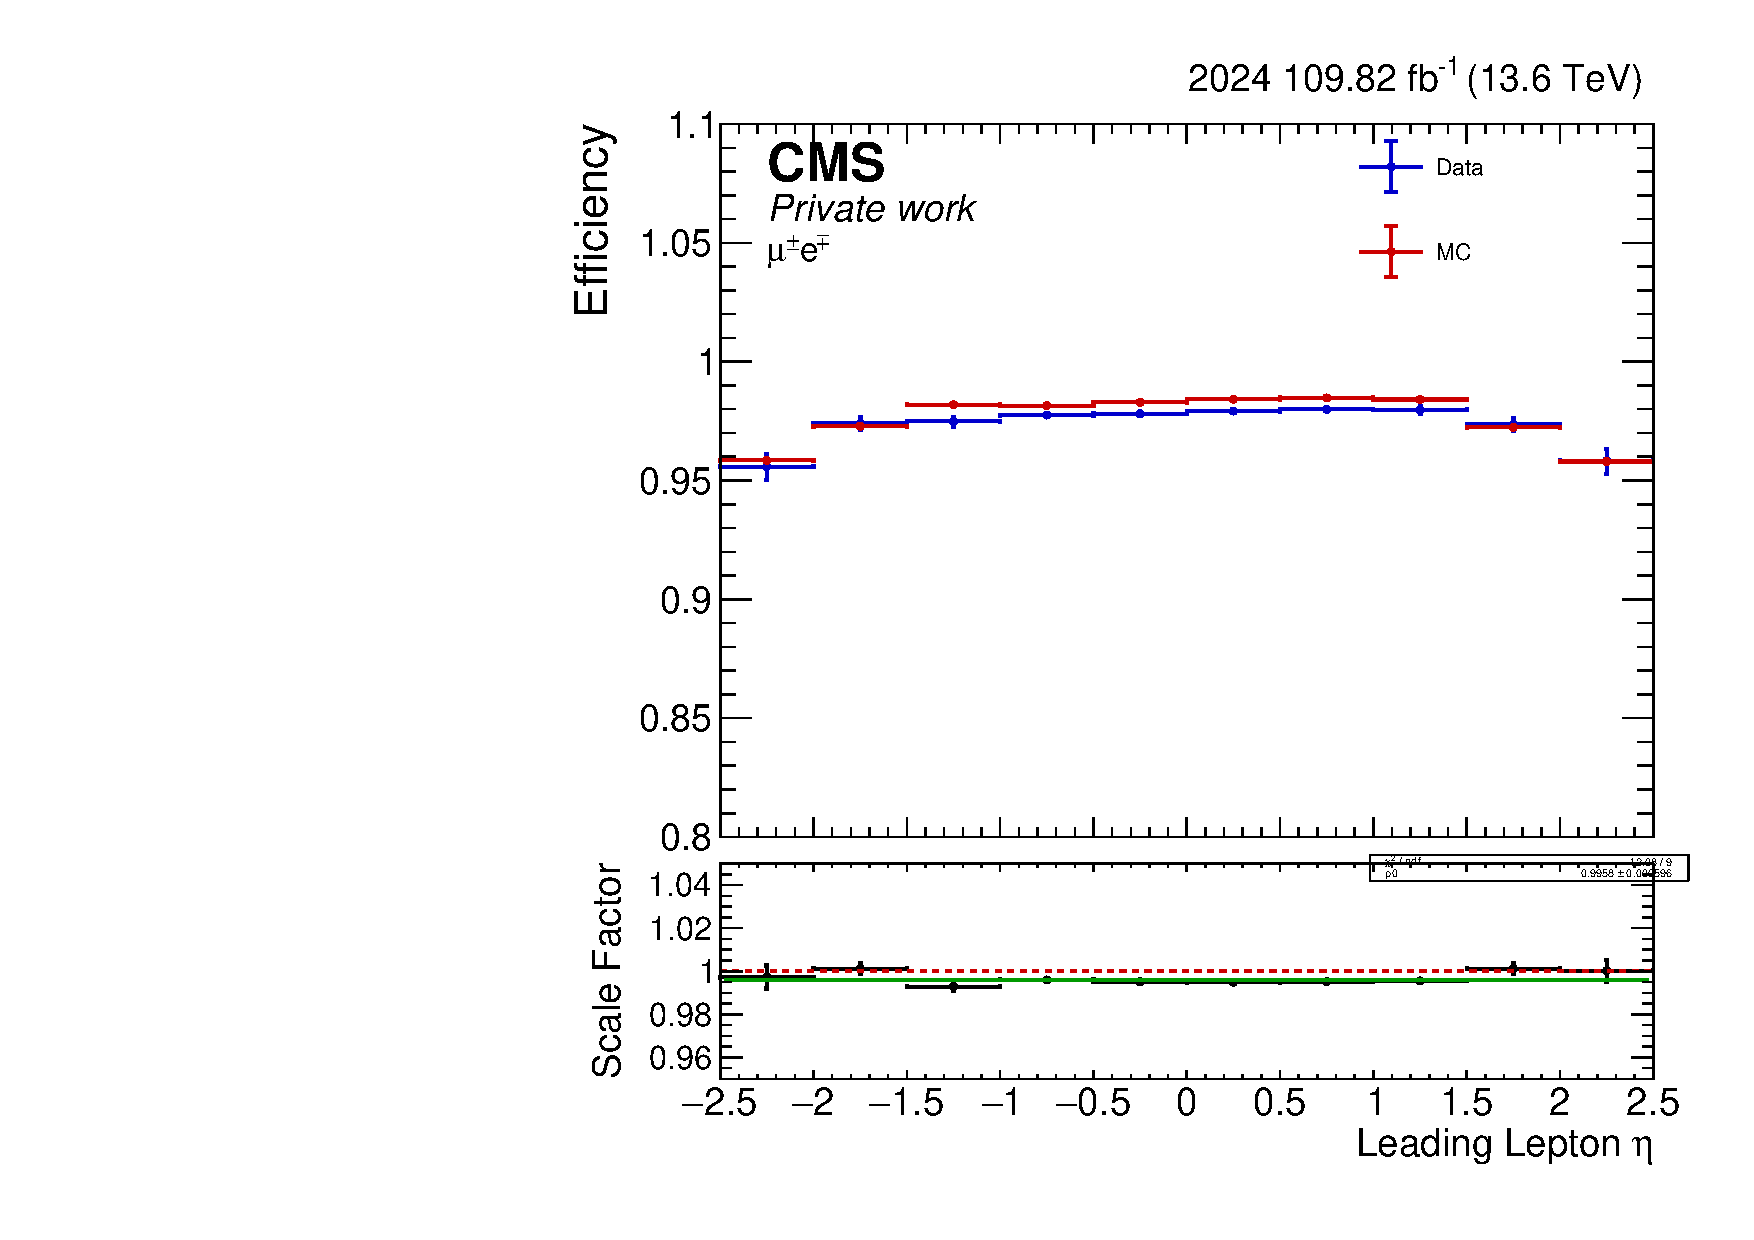
\includegraphics[width=0.48\linewidth]{figures/2024/MuEl/ScaleFactor/SF_Lep1eta.pdf}
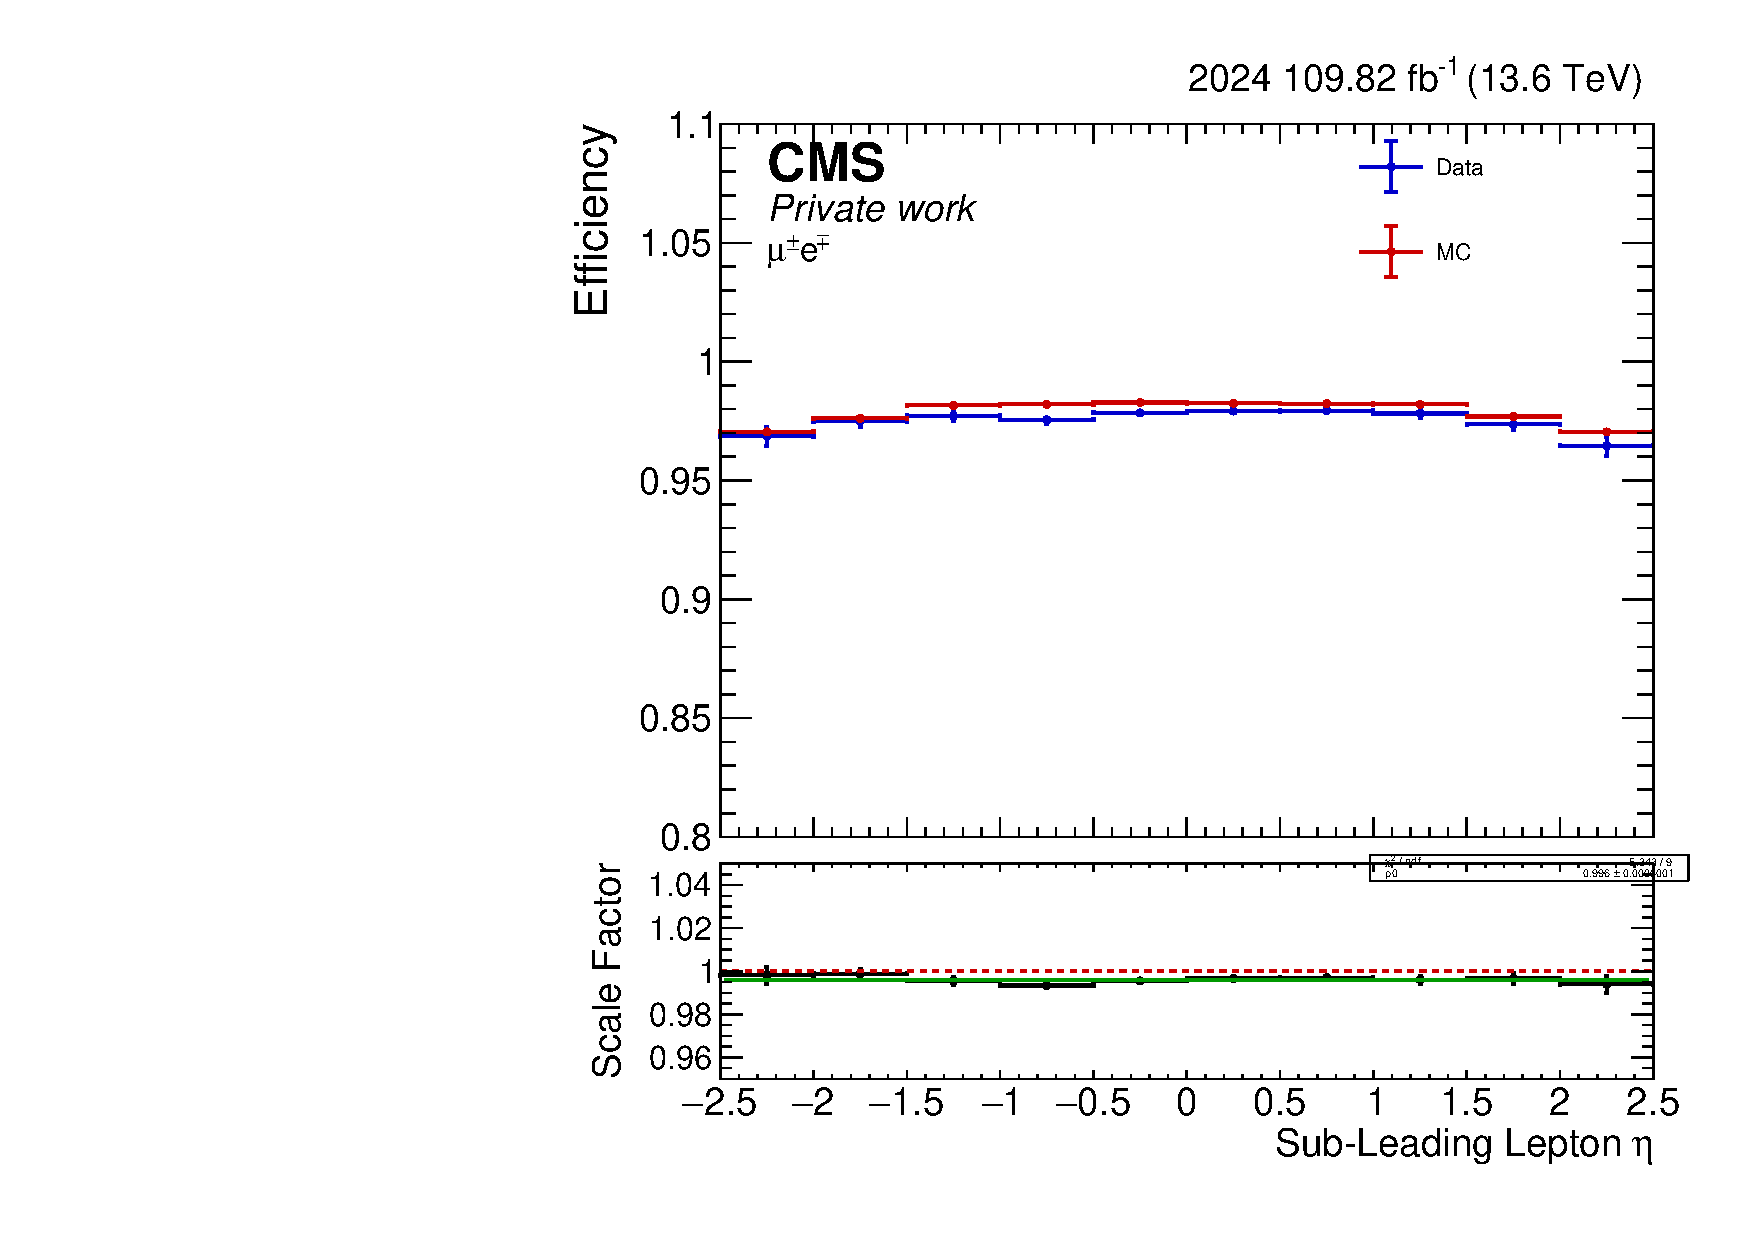
\includegraphics[width=0.48\linewidth]{figures/2024/MuEl/ScaleFactor/SF_Lep2eta.pdf}
\caption{Additional one-dimensional efficiency and SF diagnostics in the $e\mu$ channel. Variables and binning are shown on each axis.}\label{fig:diag-MuEl-SF_Lep1eta}
\end{figure}
\begin{figure}[htbp]\centering
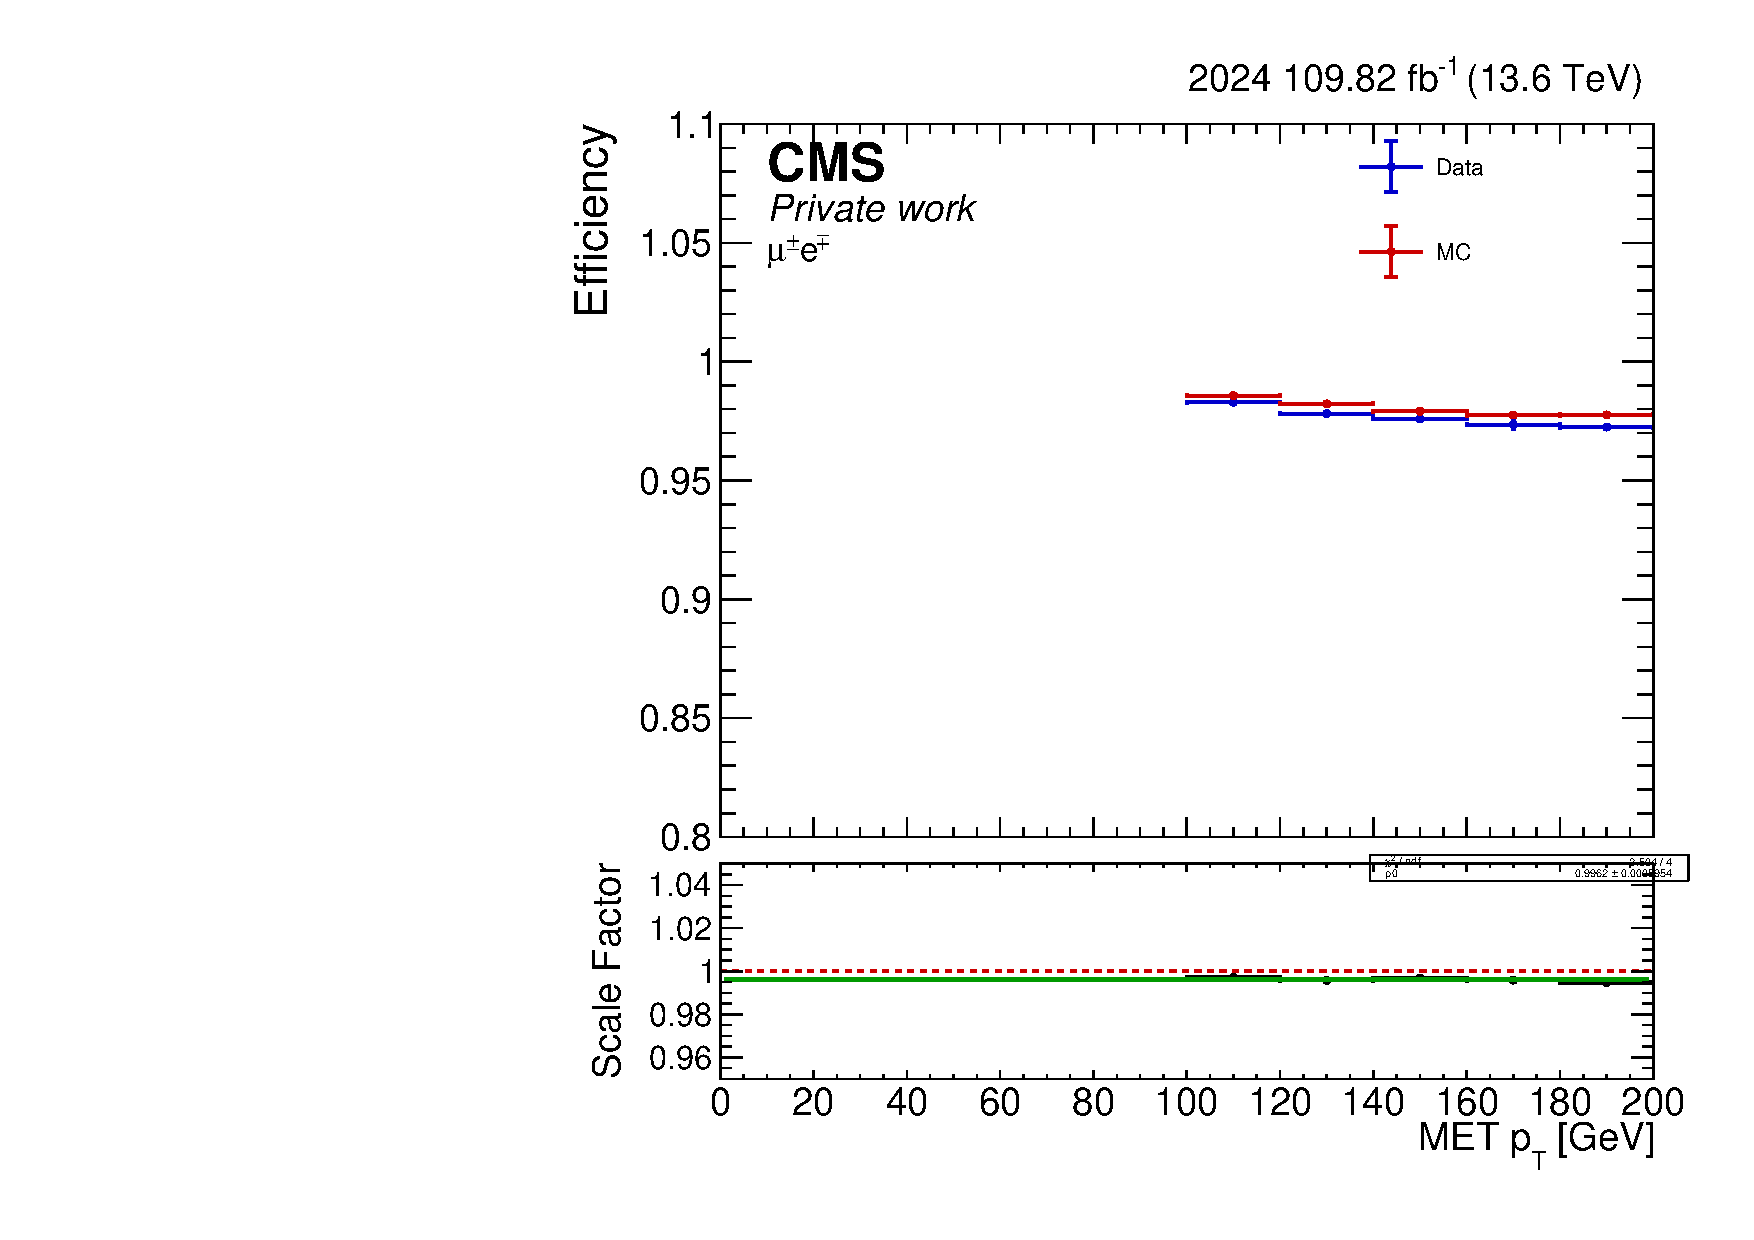
\includegraphics[width=0.48\linewidth]{figures/2024/MuEl/ScaleFactor/SF_METpt.pdf}
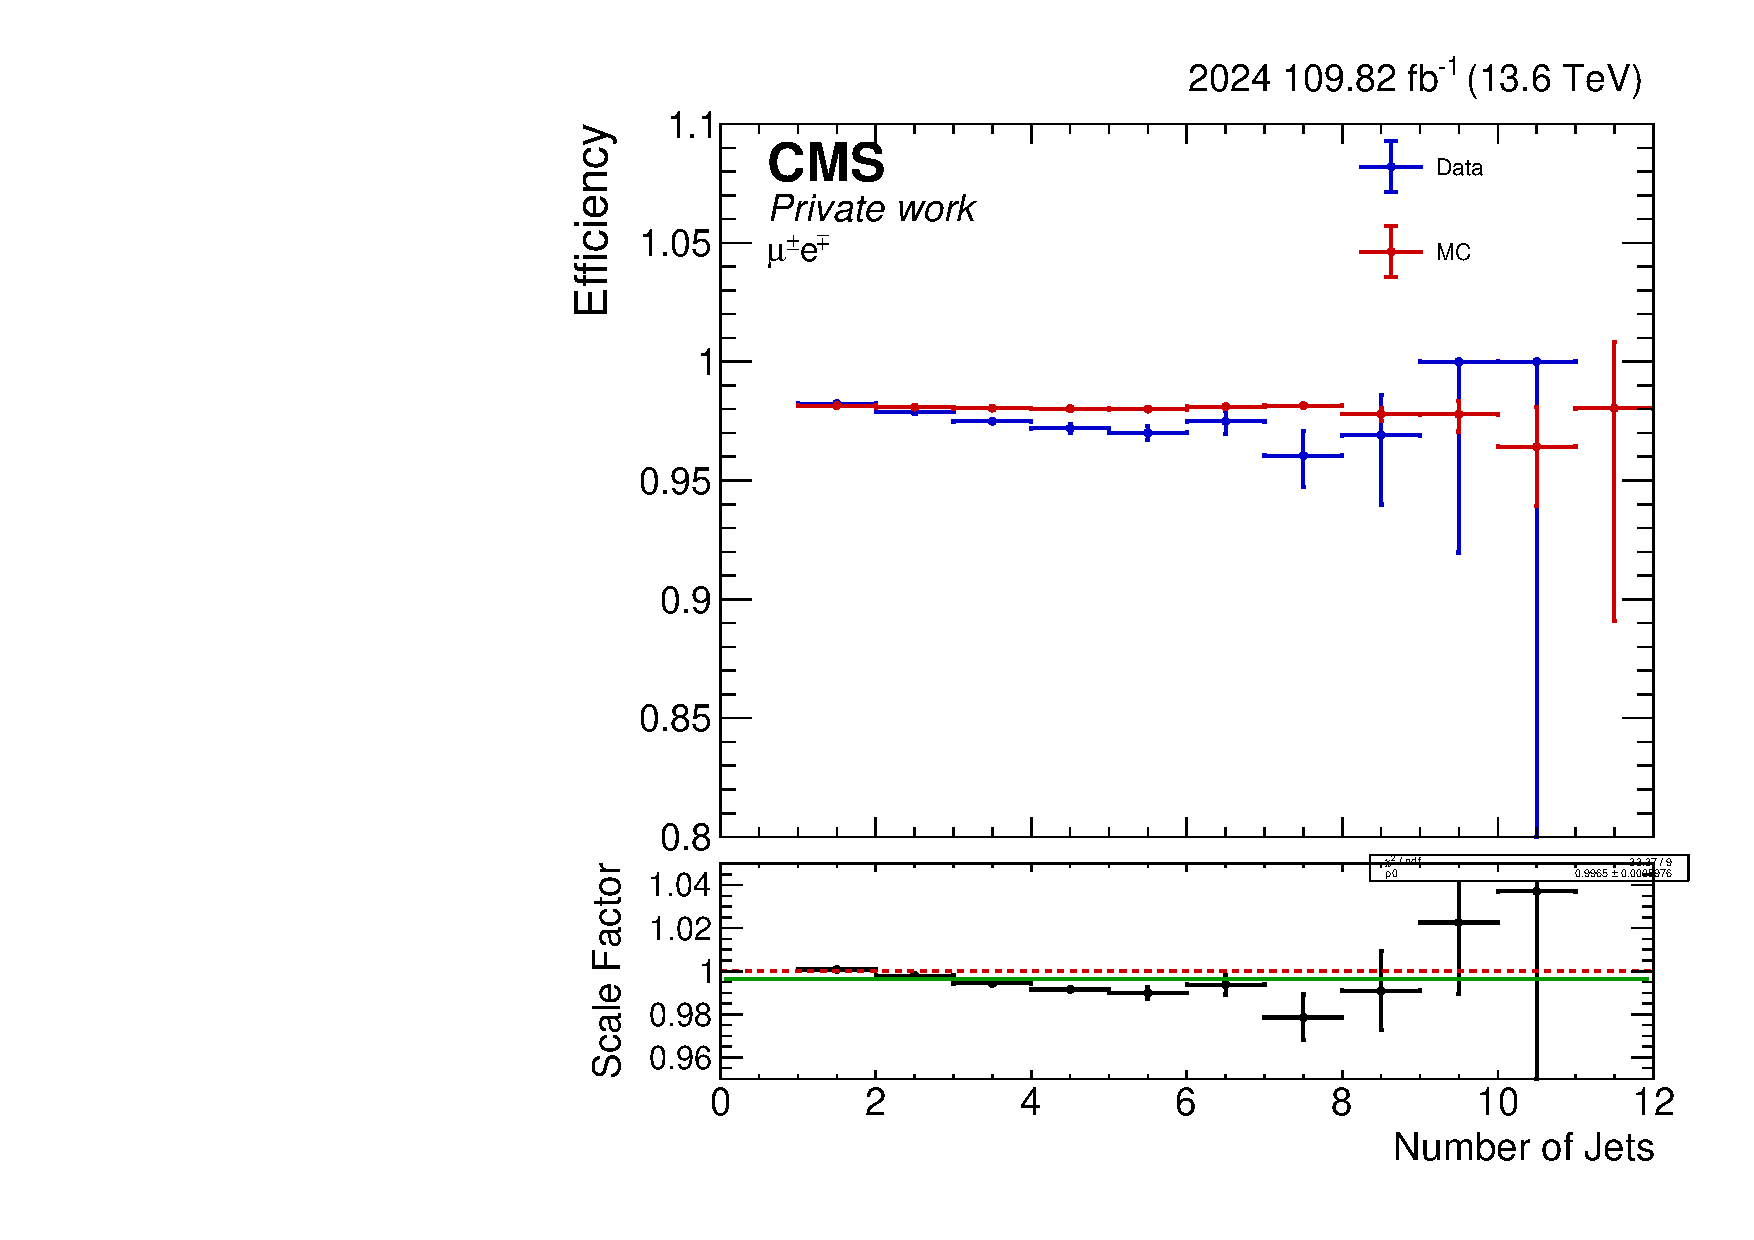
\includegraphics[width=0.48\linewidth]{figures/2024/MuEl/ScaleFactor/SF_Num_Jets.pdf}
\caption{Additional one-dimensional efficiency and SF diagnostics in the $e\mu$ channel. Variables and binning are shown on each axis.}\label{fig:diag-MuEl-SF_METpt}
\end{figure}
\begin{figure}[htbp]\centering
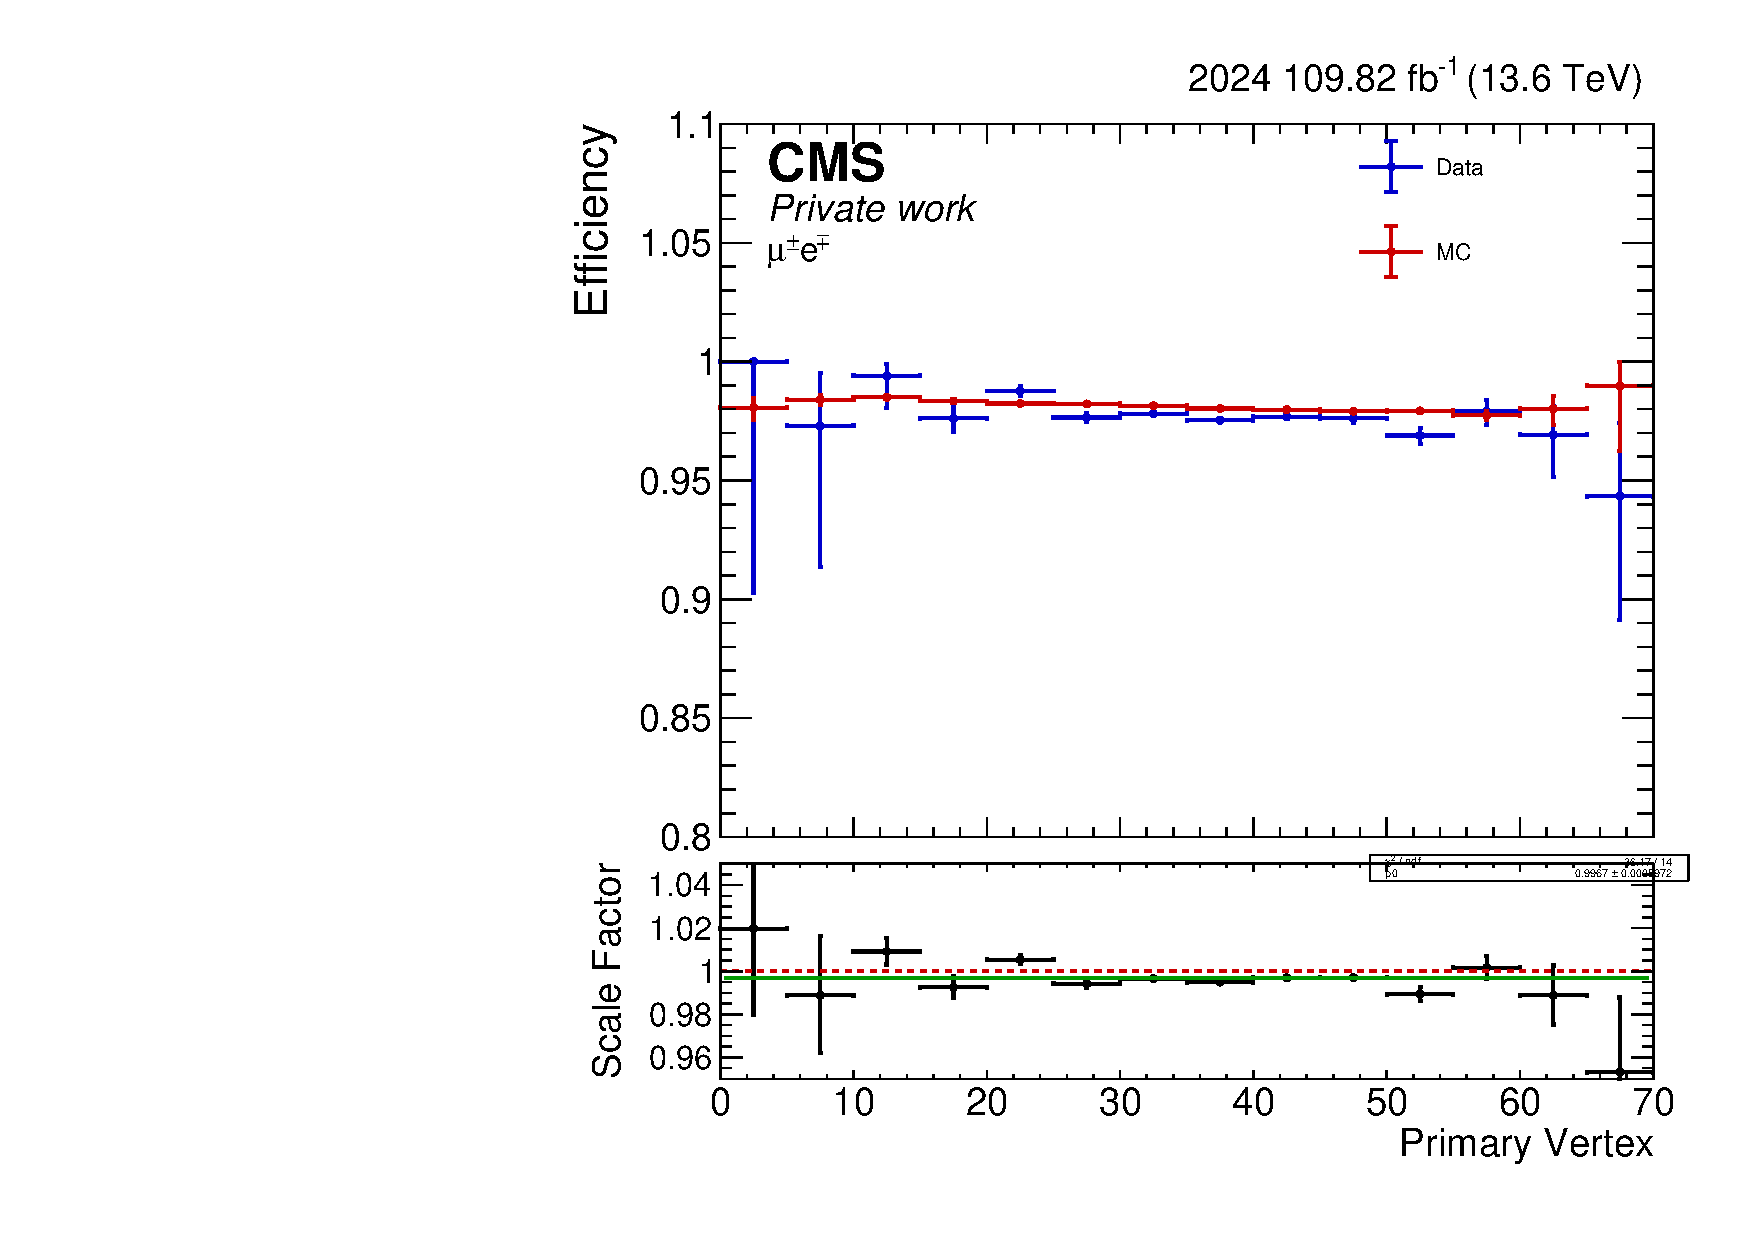
\includegraphics[width=0.48\linewidth]{figures/2024/MuEl/ScaleFactor/SF_Num_PV.pdf}
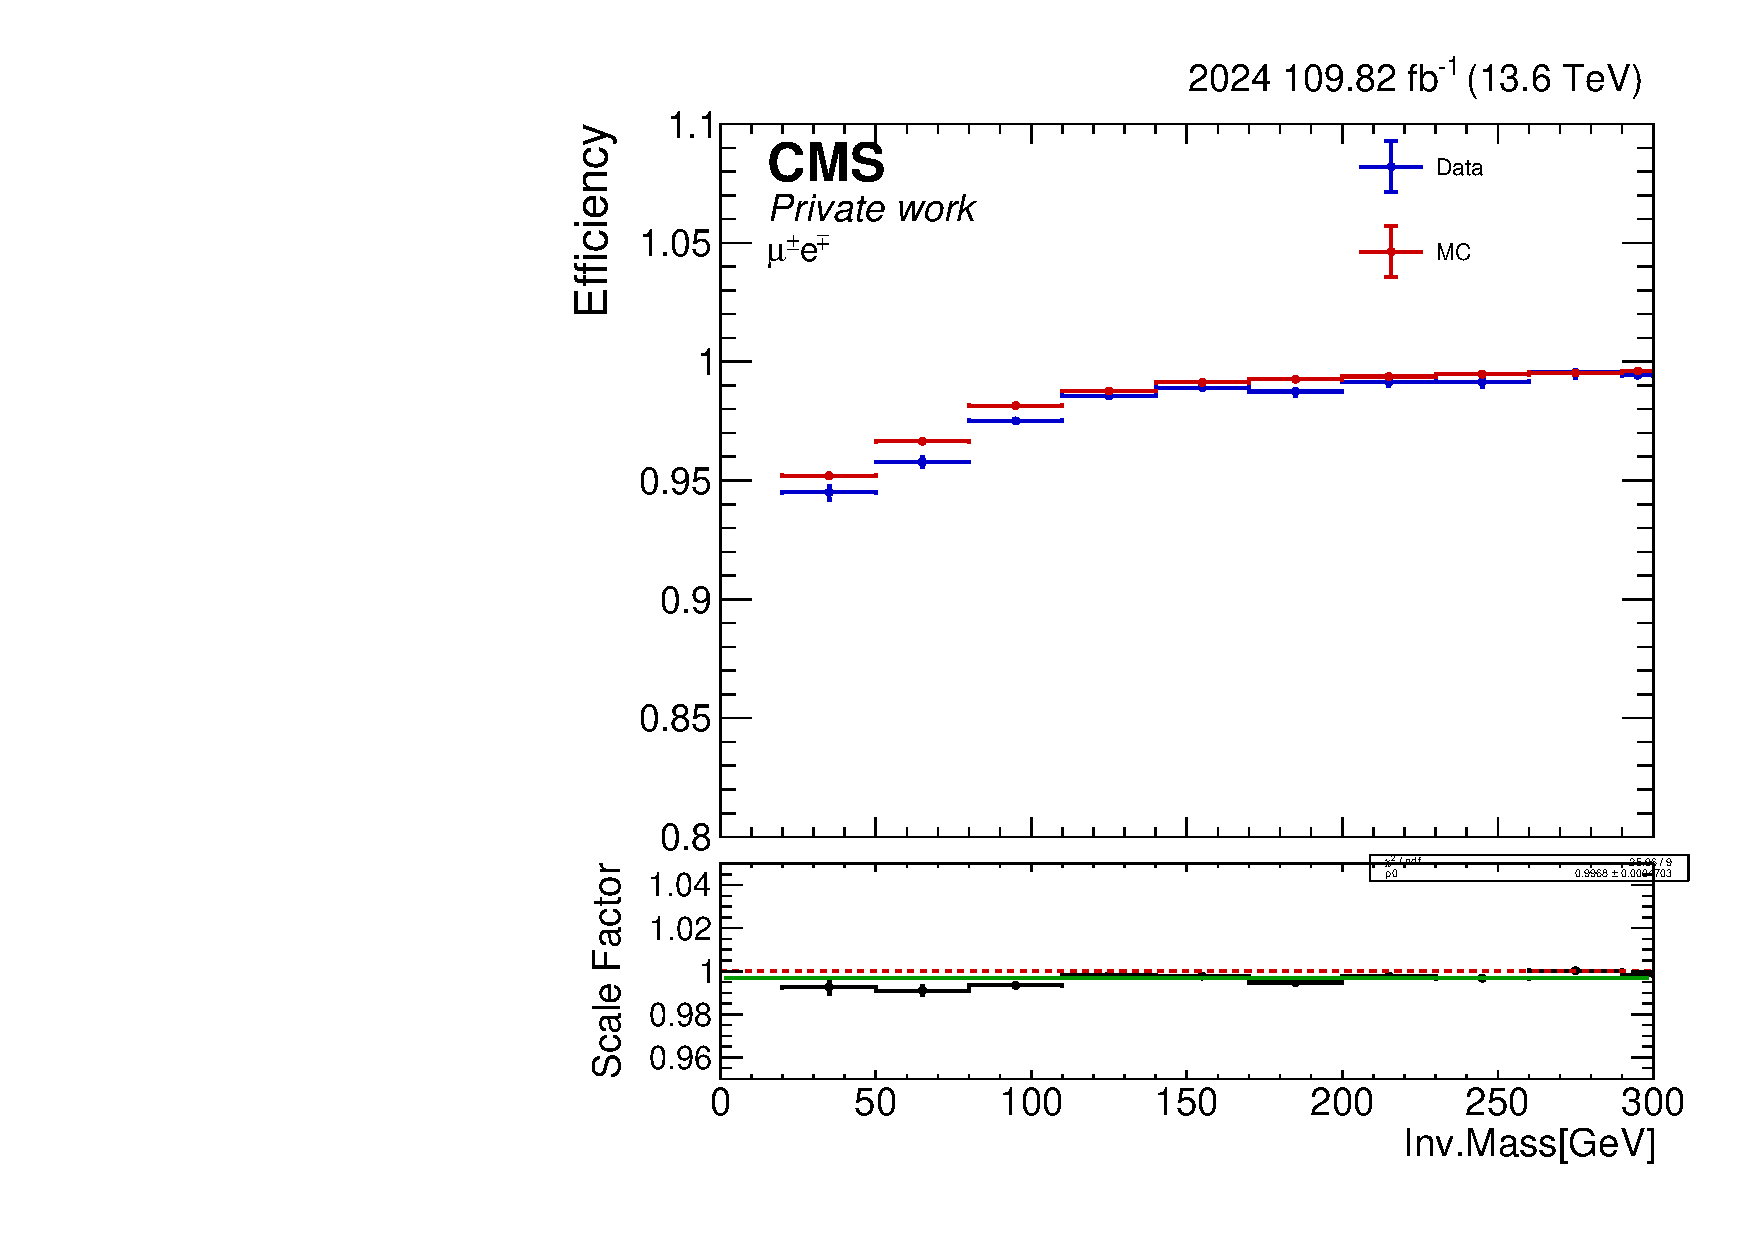
\includegraphics[width=0.48\linewidth]{figures/2024/MuEl/ScaleFactor/SF_DiLepMass.pdf}
\caption{Additional one-dimensional efficiency and SF diagnostics in the $e\mu$ channel. Variables and binning are shown on each axis.}\label{fig:diag-MuEl-SF_Num_PV}
\end{figure}
\begin{figure}[htbp]\centering
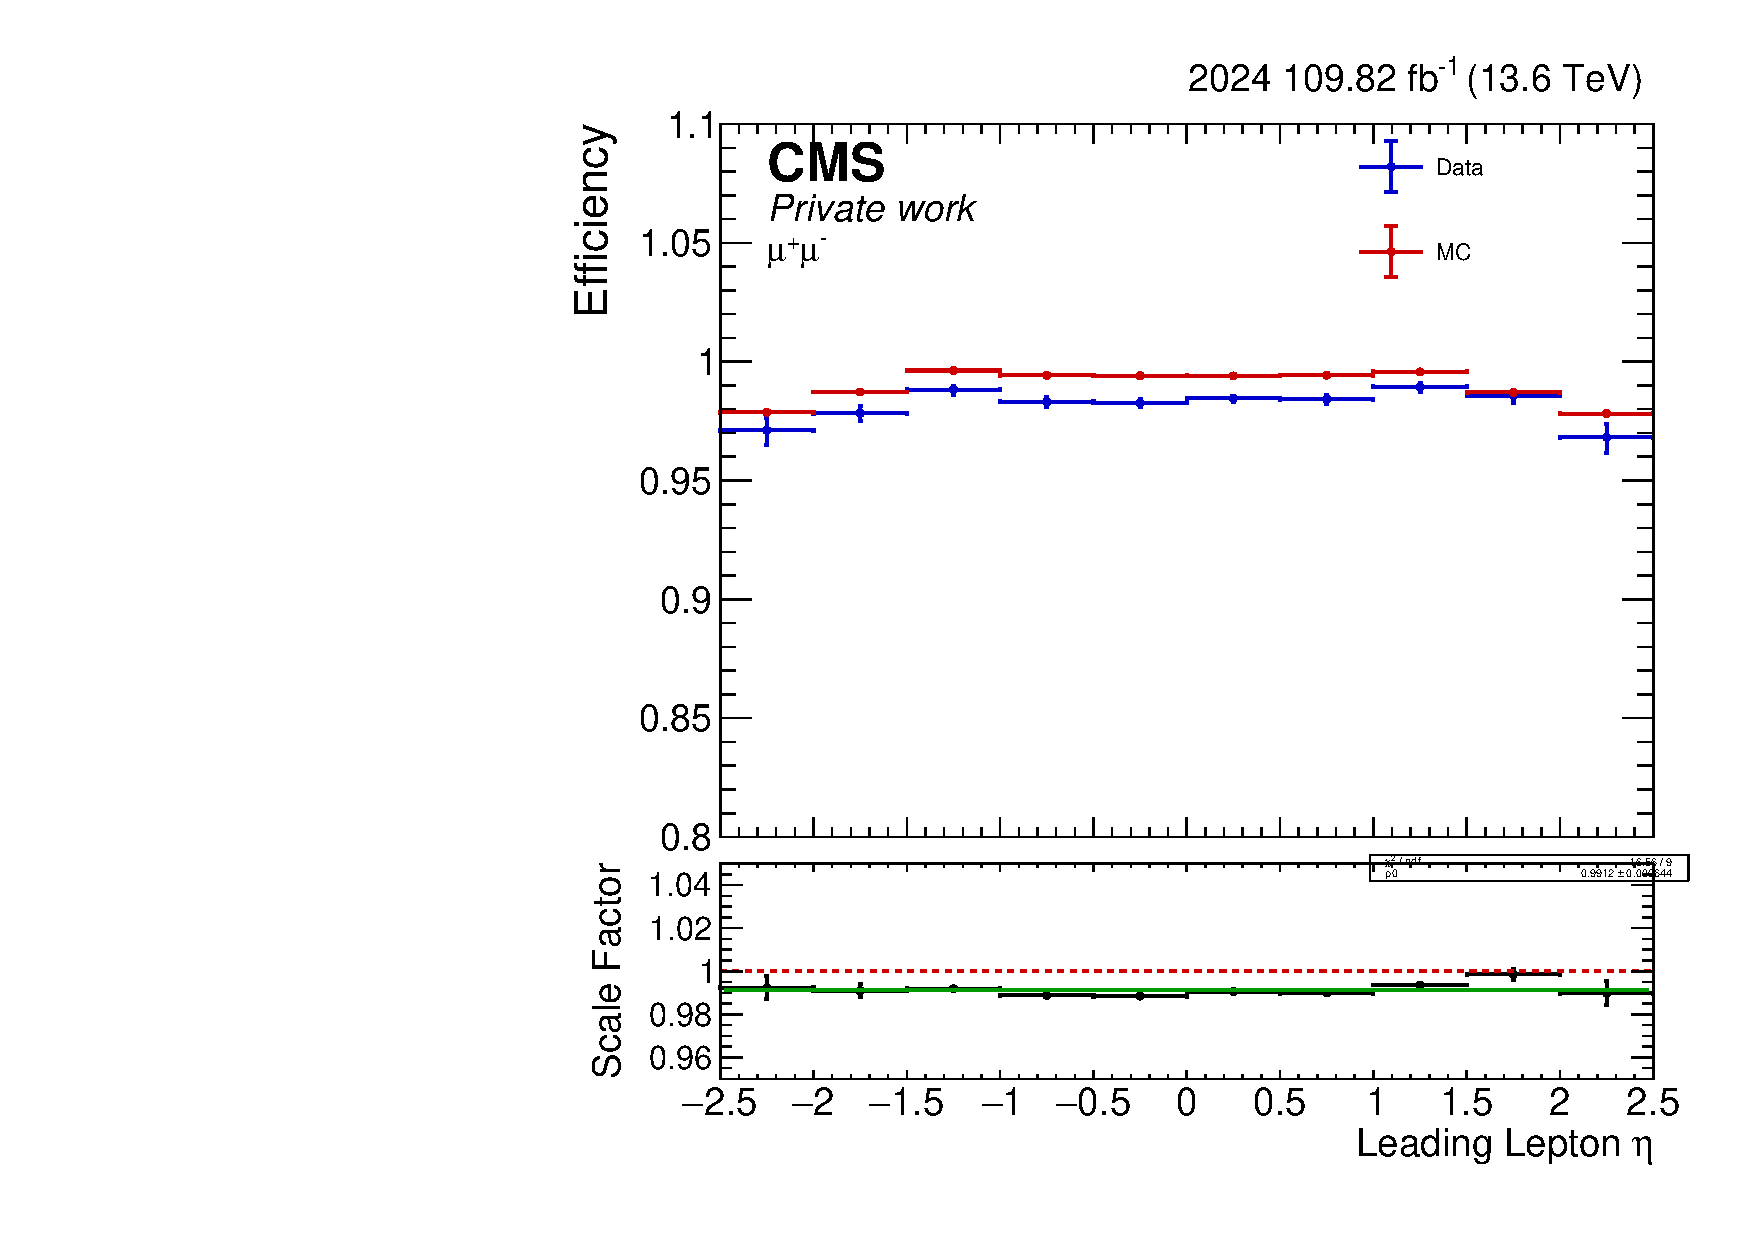
\includegraphics[width=0.48\linewidth]{figures/2024/MuMu/ScaleFactor/SF_Lep1eta.pdf}
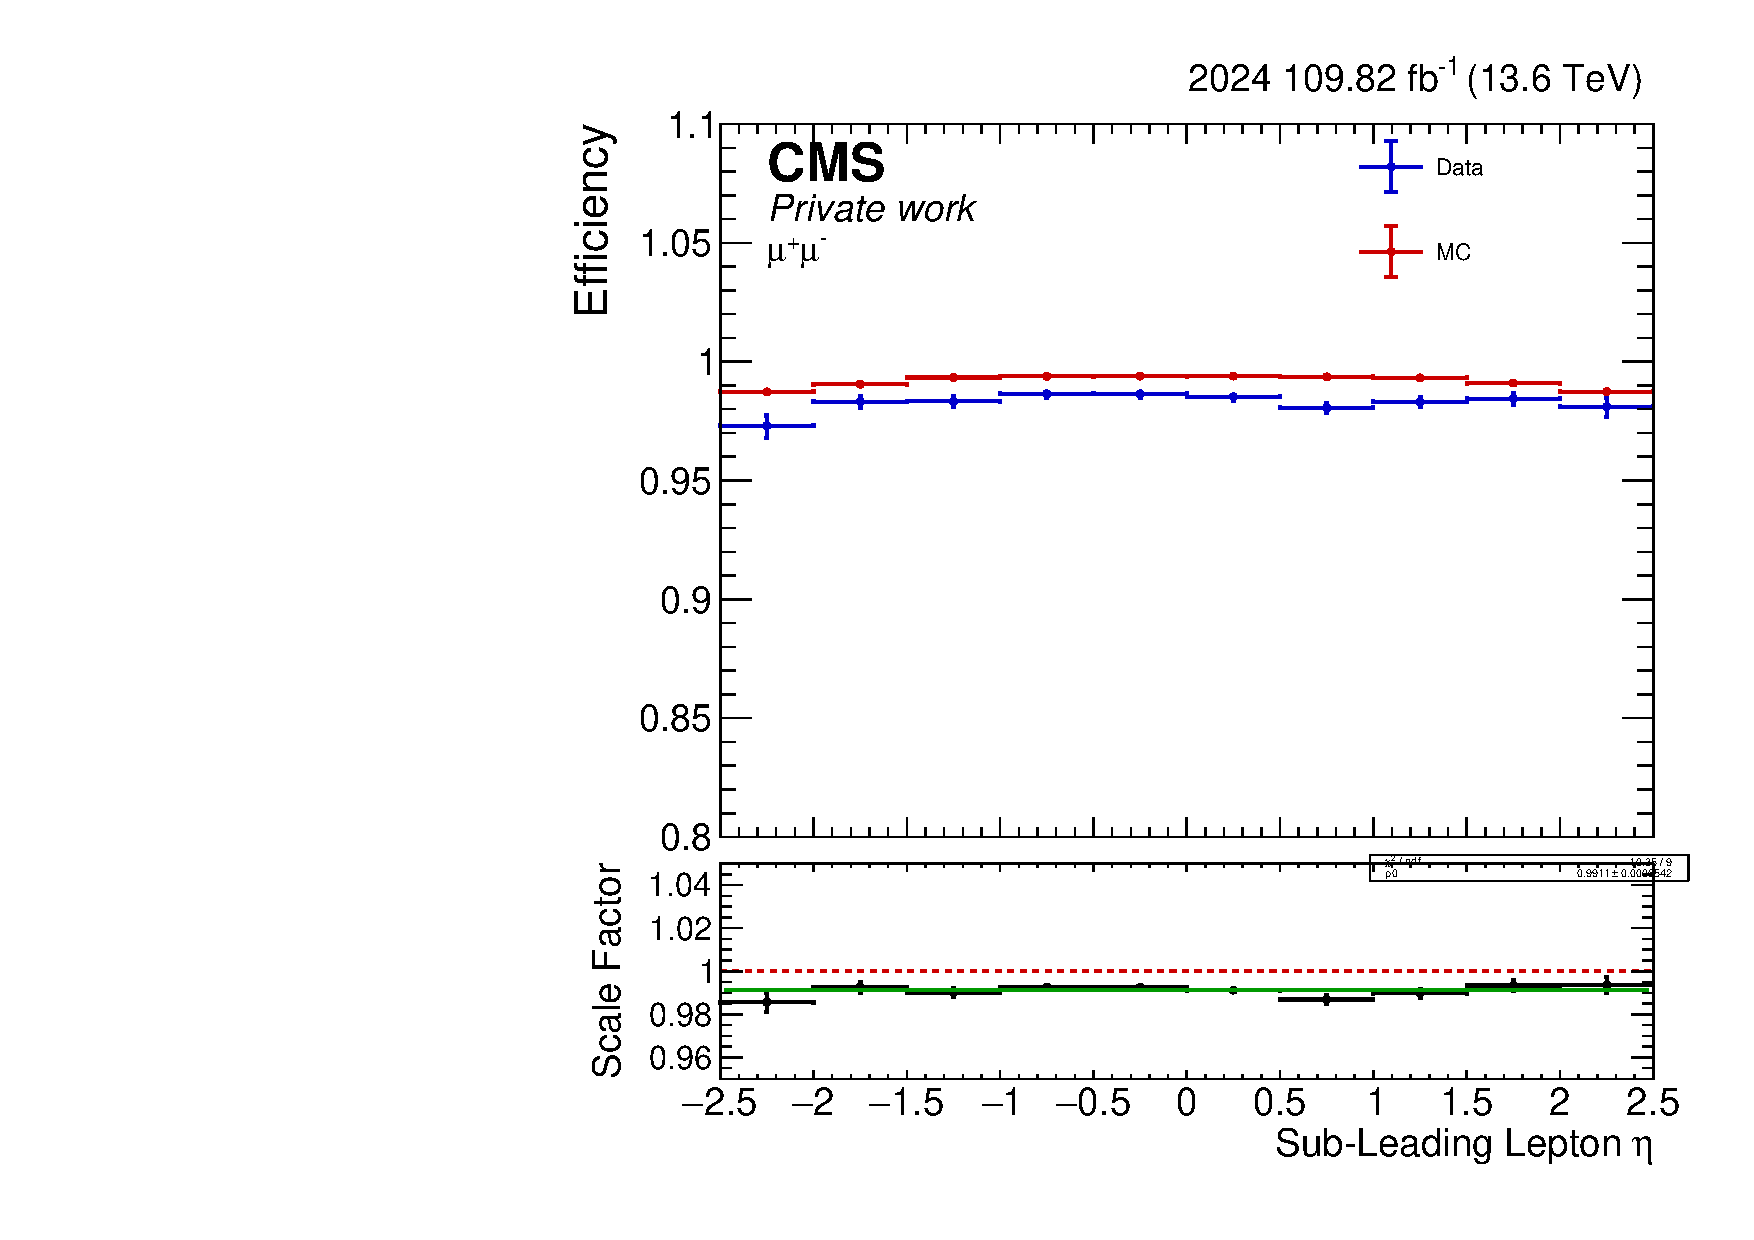
\includegraphics[width=0.48\linewidth]{figures/2024/MuMu/ScaleFactor/SF_Lep2eta.pdf}
\caption{Additional one-dimensional efficiency and SF diagnostics in the $\mu\mu$ channel. Variables and binning are shown on each axis.}\label{fig:diag-MuMu-SF_Lep1eta}
\end{figure}
\begin{figure}[htbp]\centering
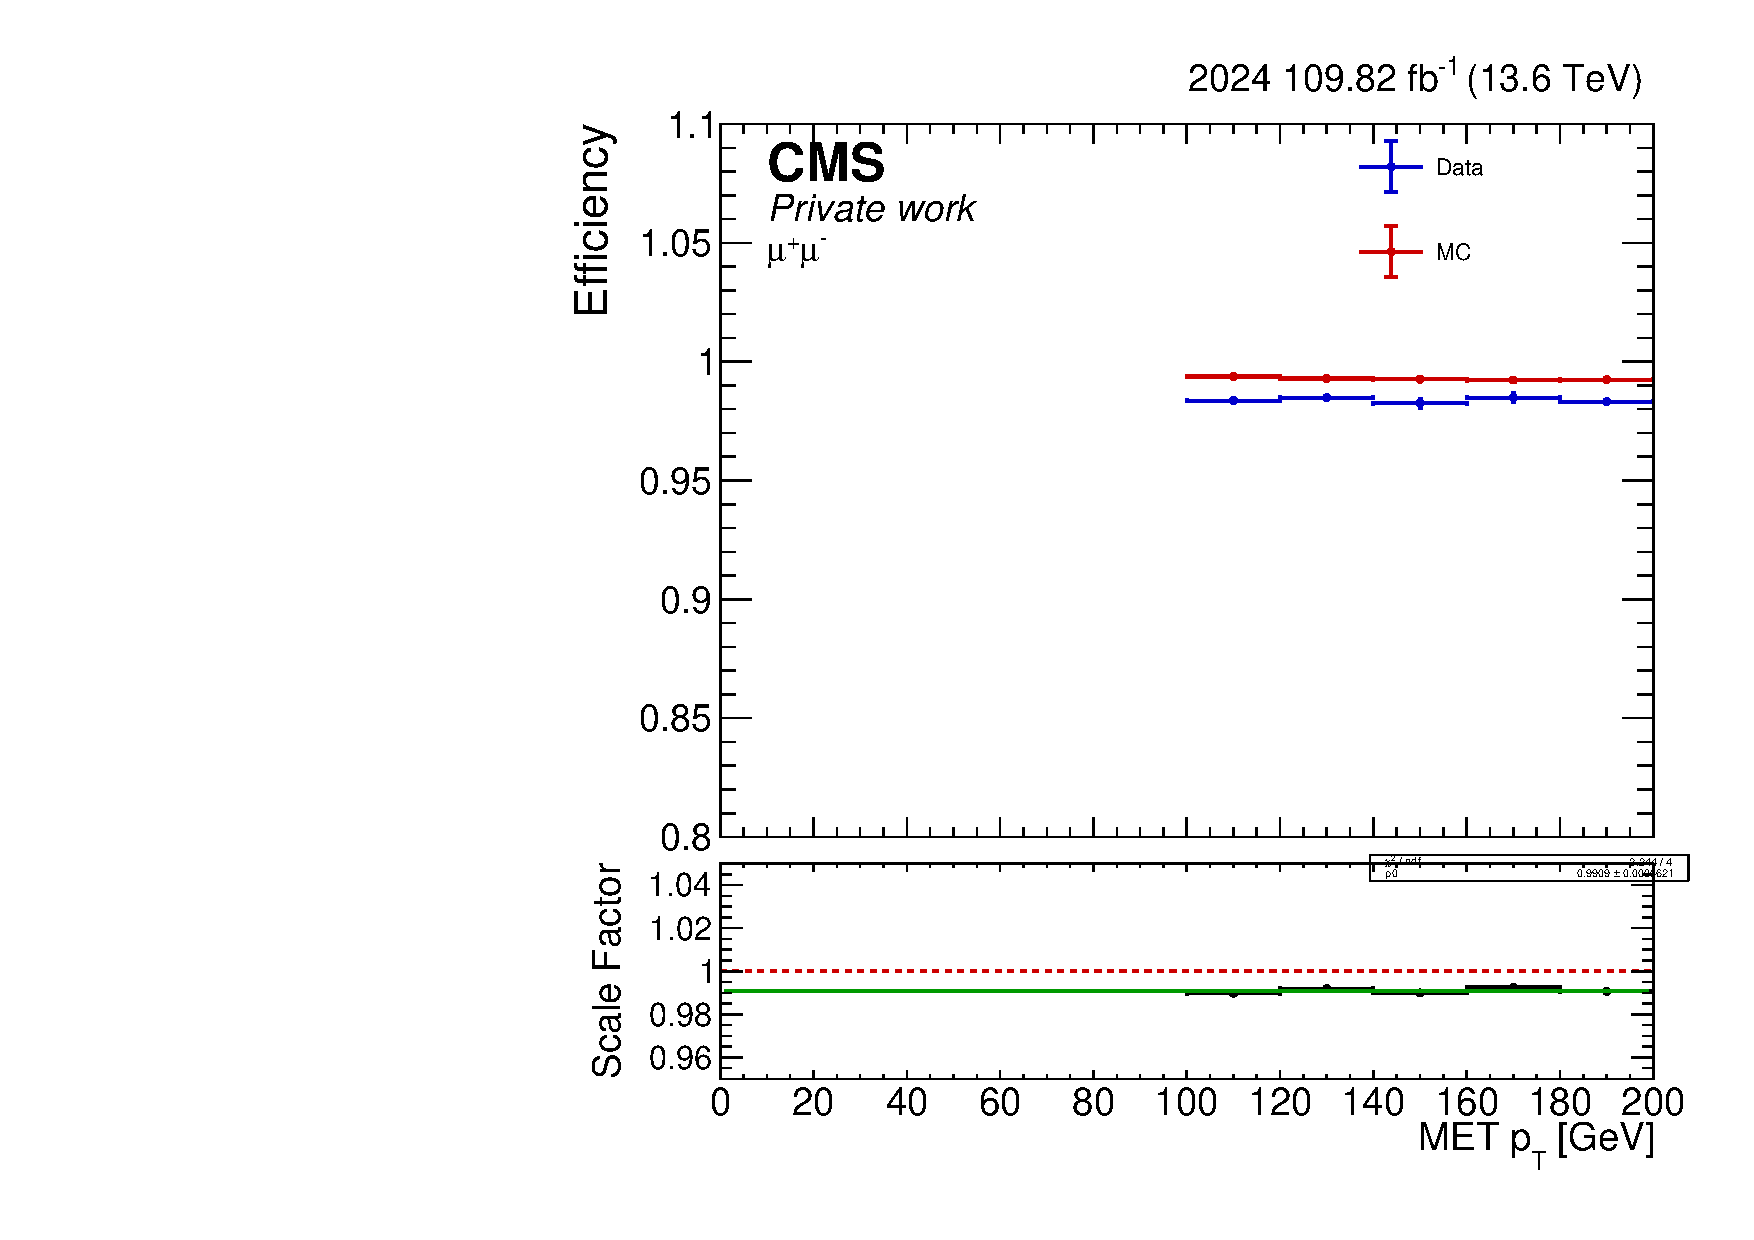
\includegraphics[width=0.48\linewidth]{figures/2024/MuMu/ScaleFactor/SF_METpt.pdf}
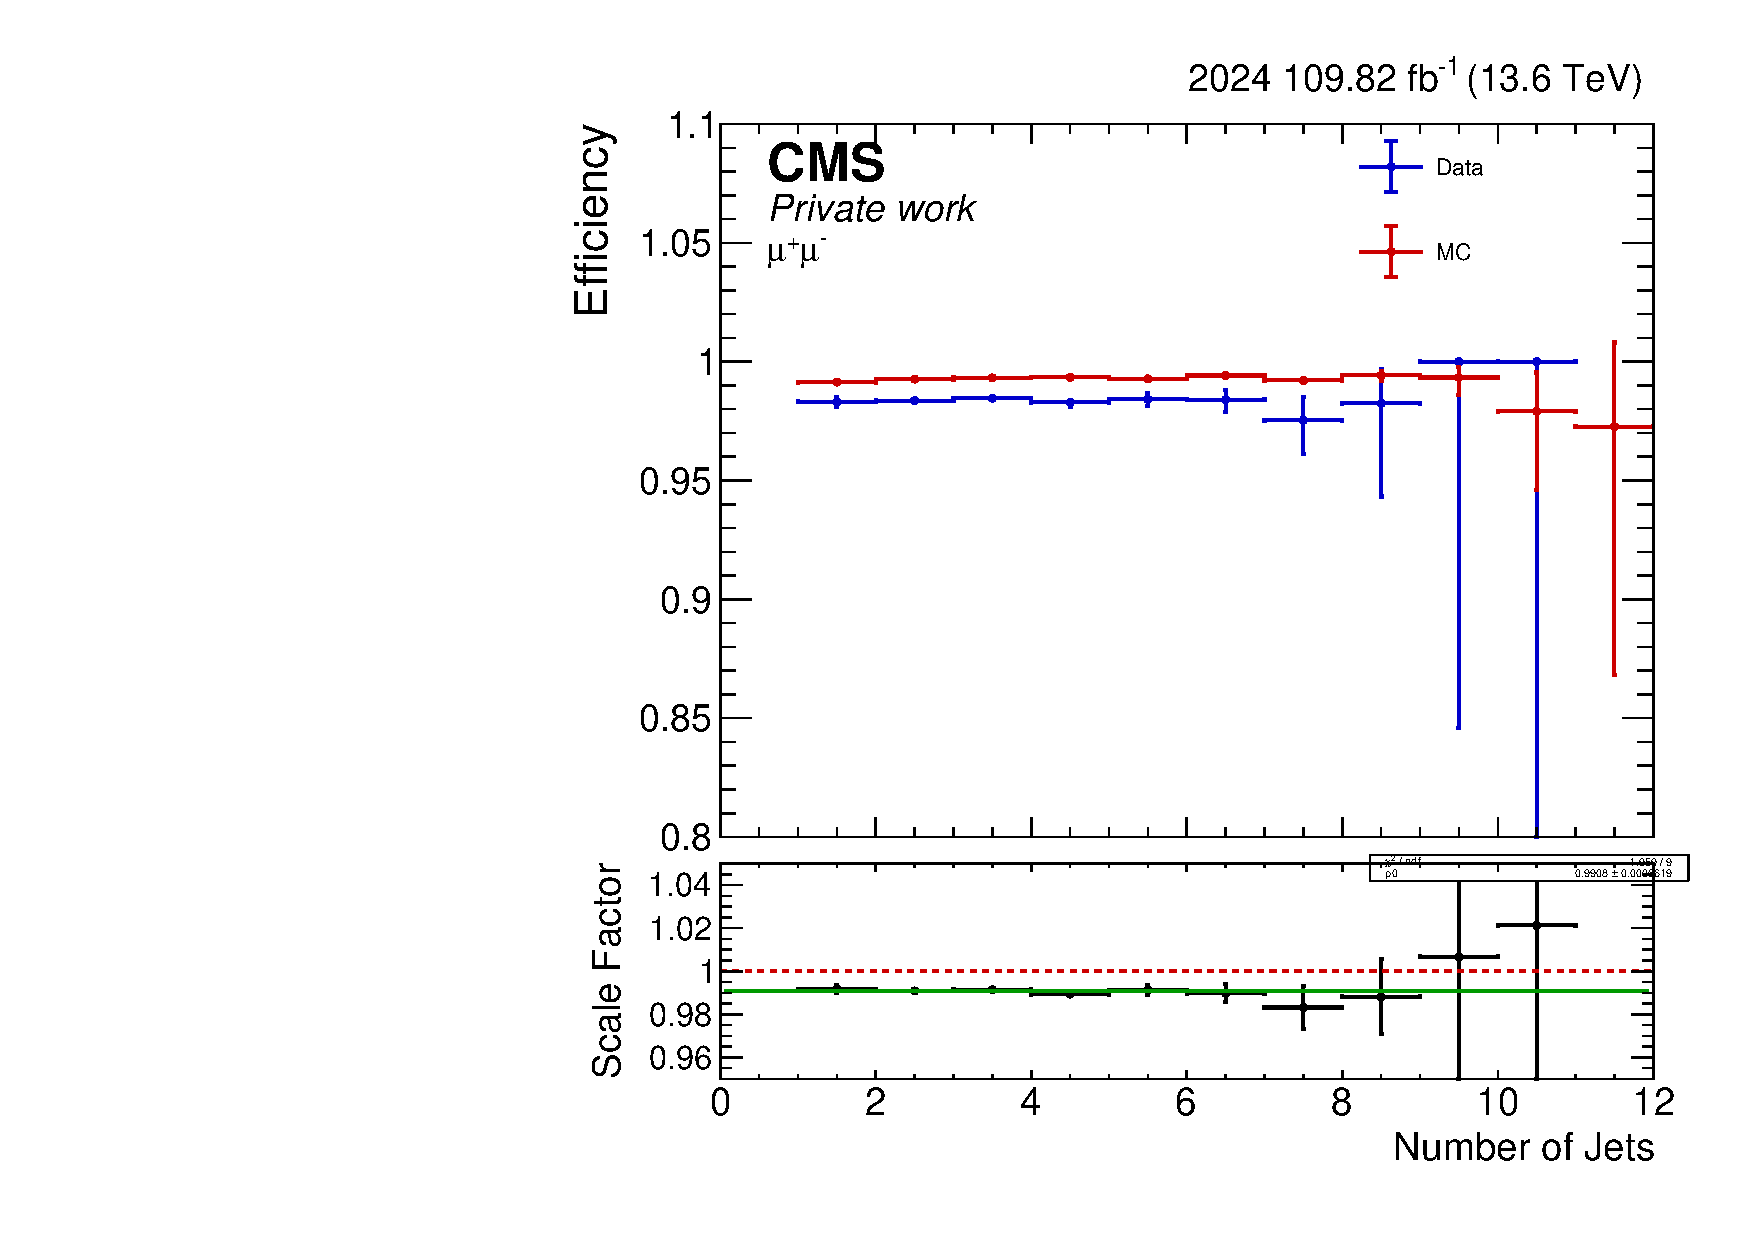
\includegraphics[width=0.48\linewidth]{figures/2024/MuMu/ScaleFactor/SF_Num_Jets.pdf}
\caption{Additional one-dimensional efficiency and SF diagnostics in the $\mu\mu$ channel. Variables and binning are shown on each axis.}\label{fig:diag-MuMu-SF_METpt}
\end{figure}
\begin{figure}[htbp]\centering
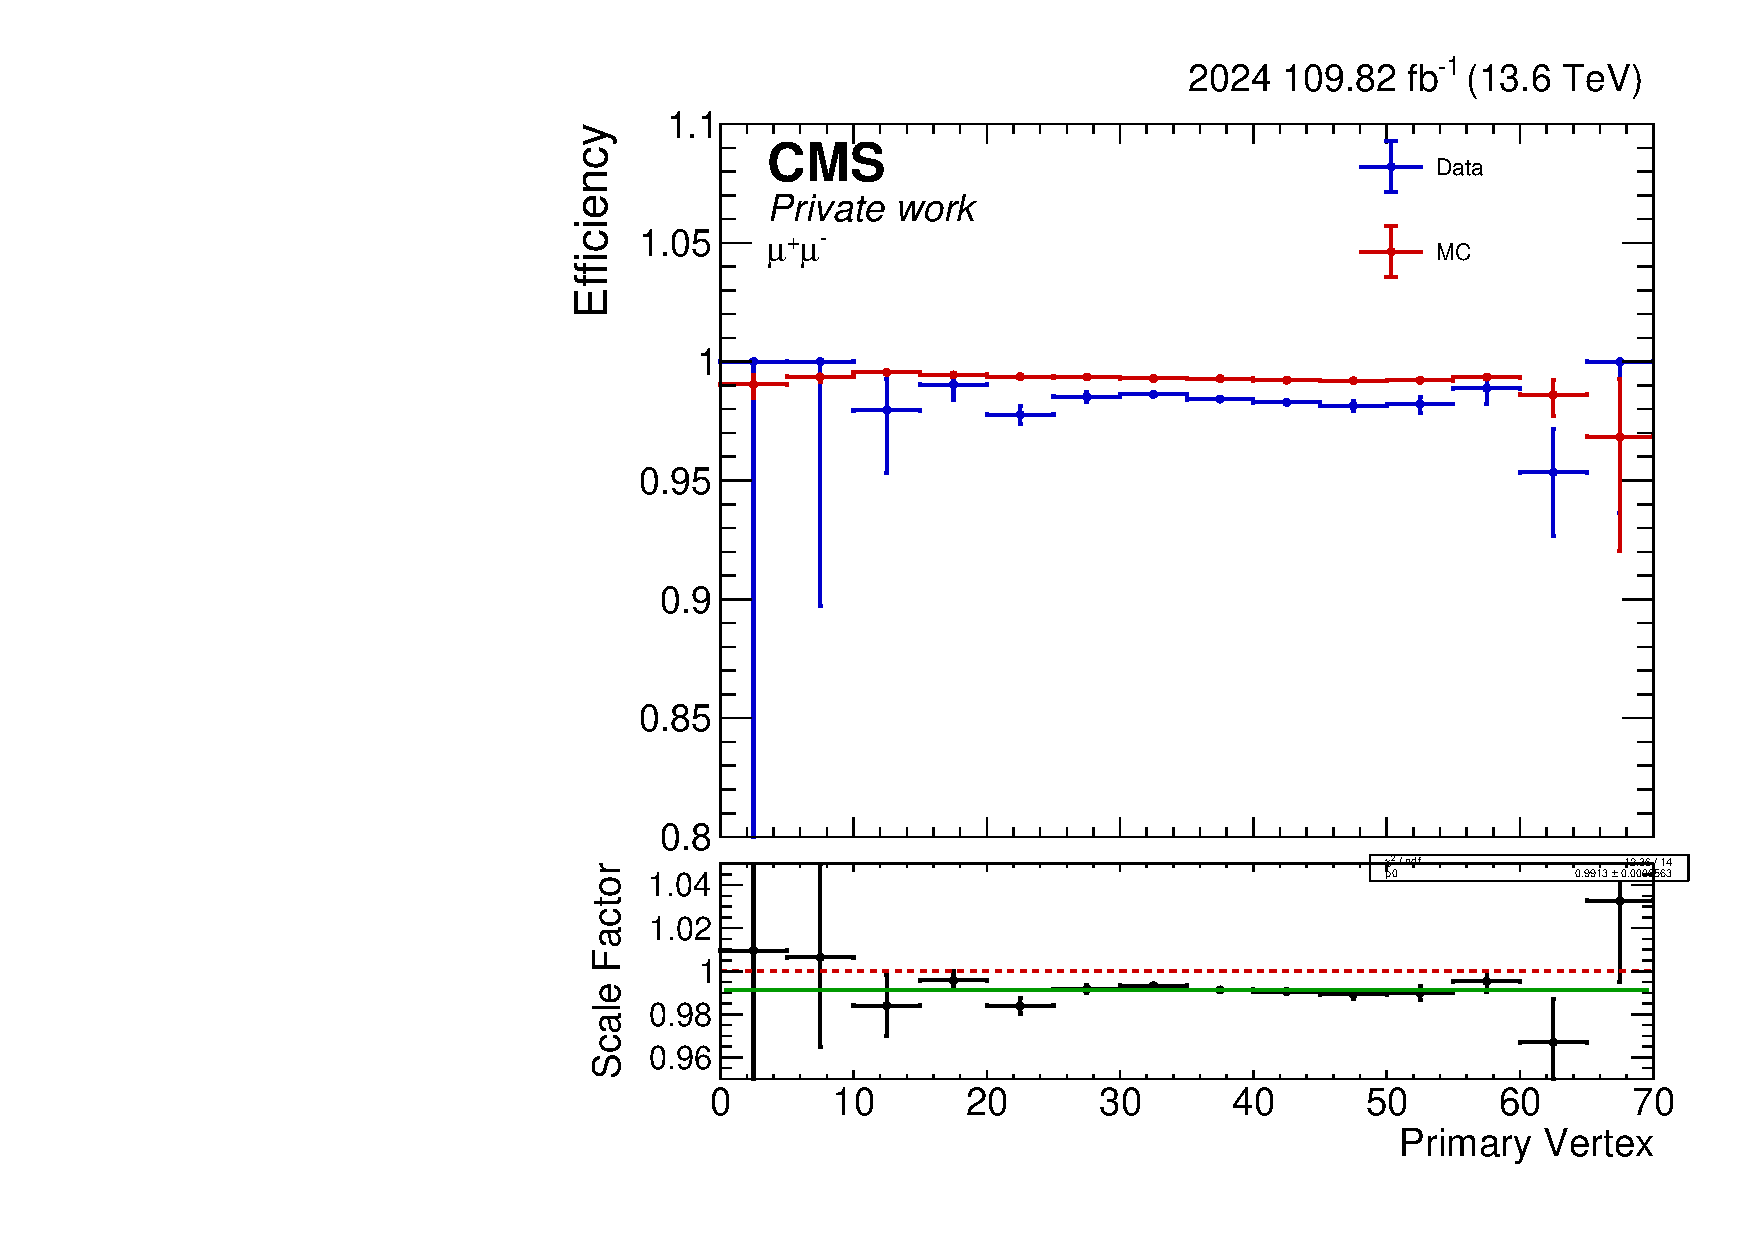
\includegraphics[width=0.48\linewidth]{figures/2024/MuMu/ScaleFactor/SF_Num_PV.pdf}
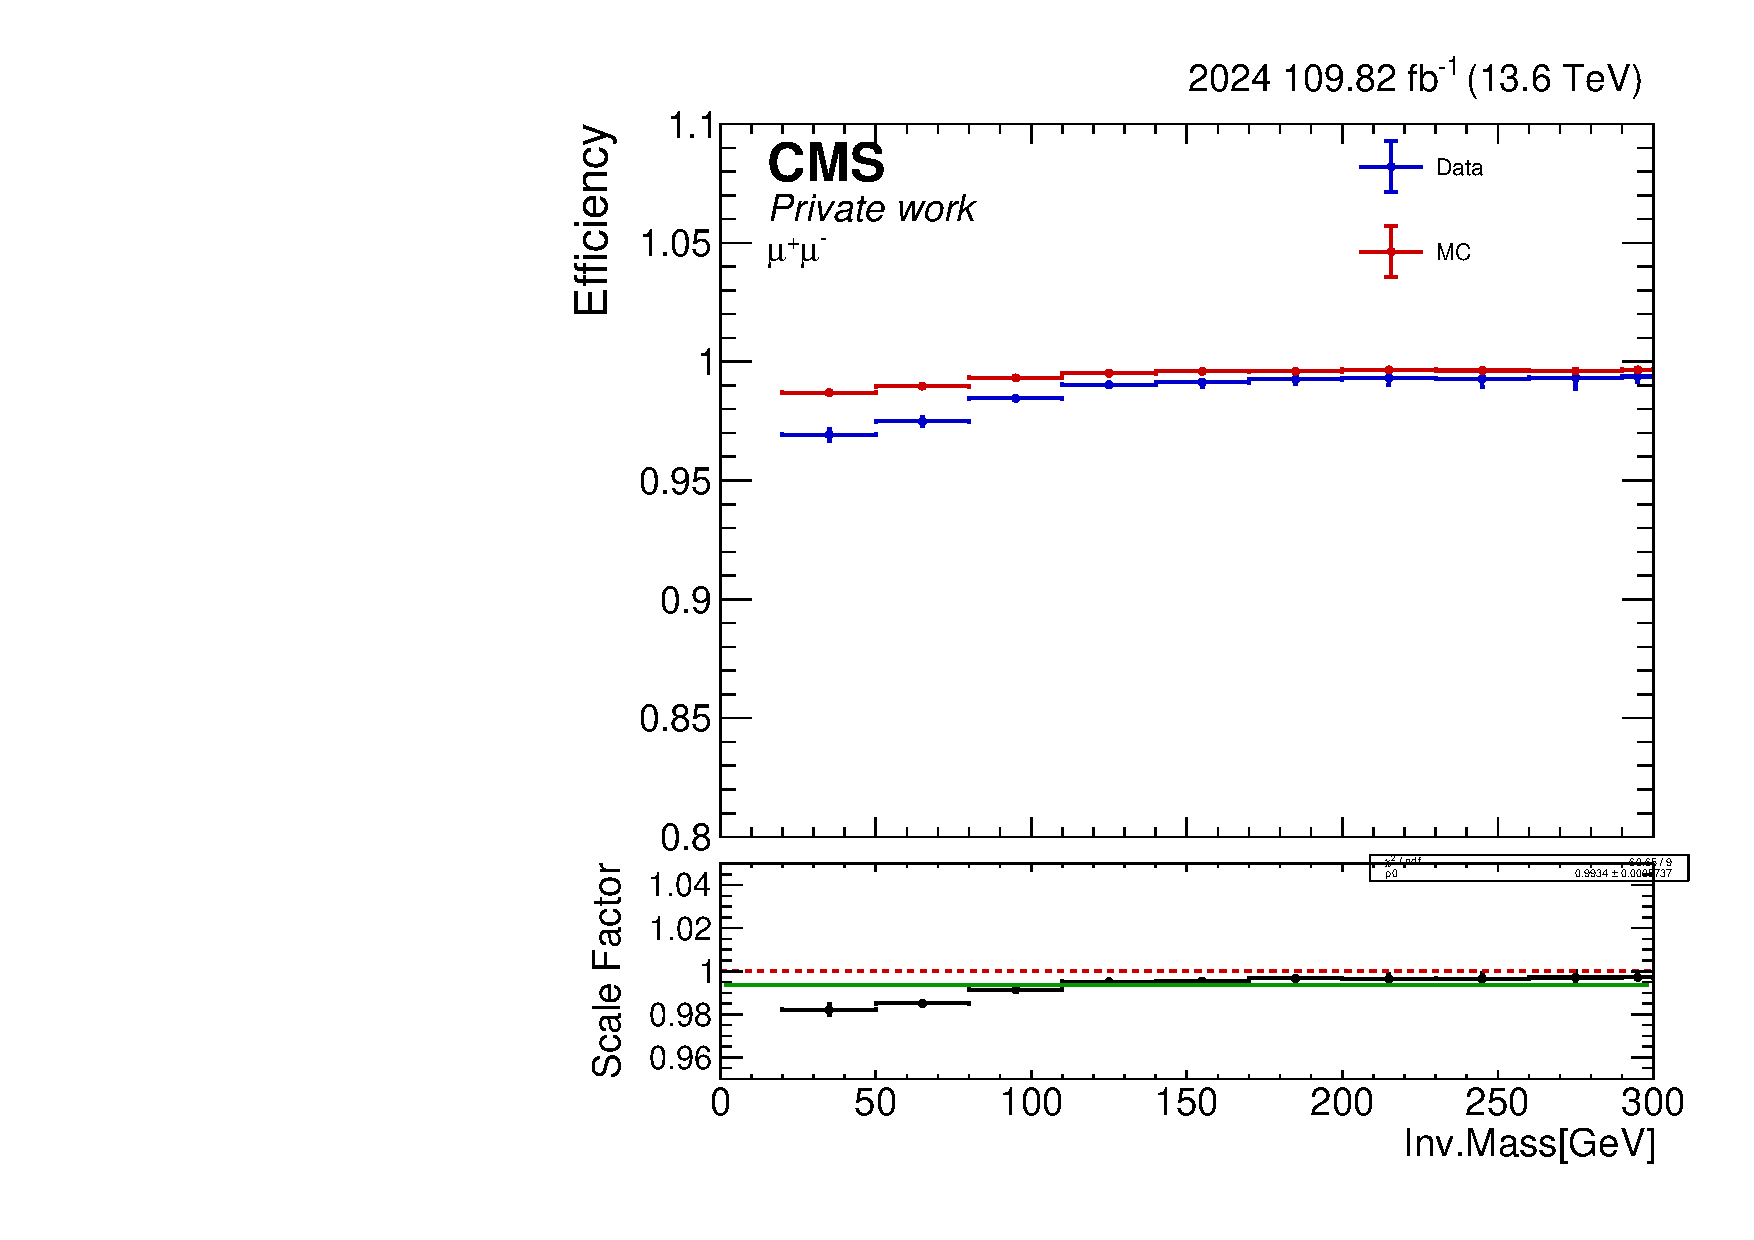
\includegraphics[width=0.48\linewidth]{figures/2024/MuMu/ScaleFactor/SF_DiLepMass.pdf}
\caption{Additional one-dimensional efficiency and SF diagnostics in the $\mu\mu$ channel. Variables and binning are shown on each axis.}\label{fig:diag-MuMu-SF_Num_PV}
\end{figure}
\clearpage\section{2024: detailed uncertainty studies}\label{app:studies}
\begin{figure}[htbp]\centering
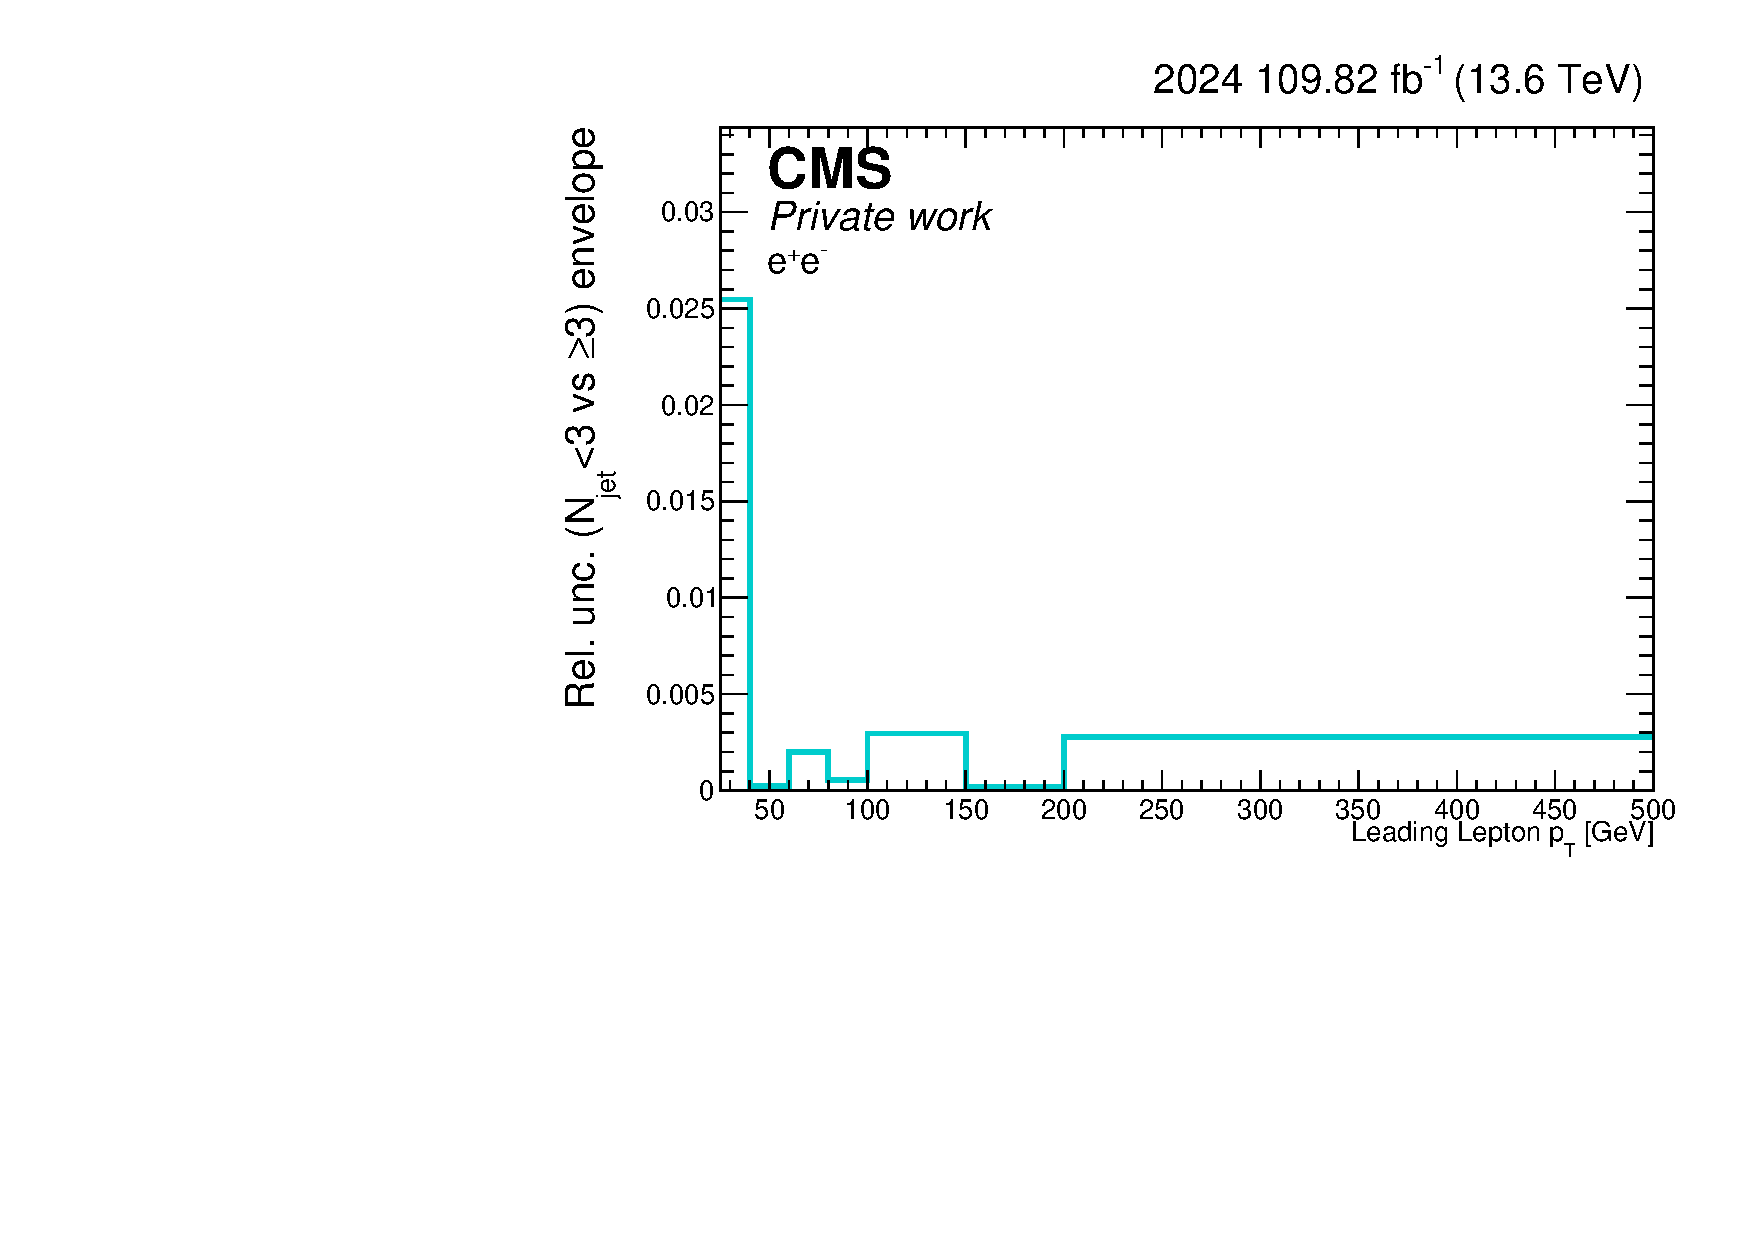
\includegraphics[width=0.48\linewidth]{figures/2024/ElEl/Jet_Topology_Uncertainty/TopoJetUnc_Lep1pt.pdf}
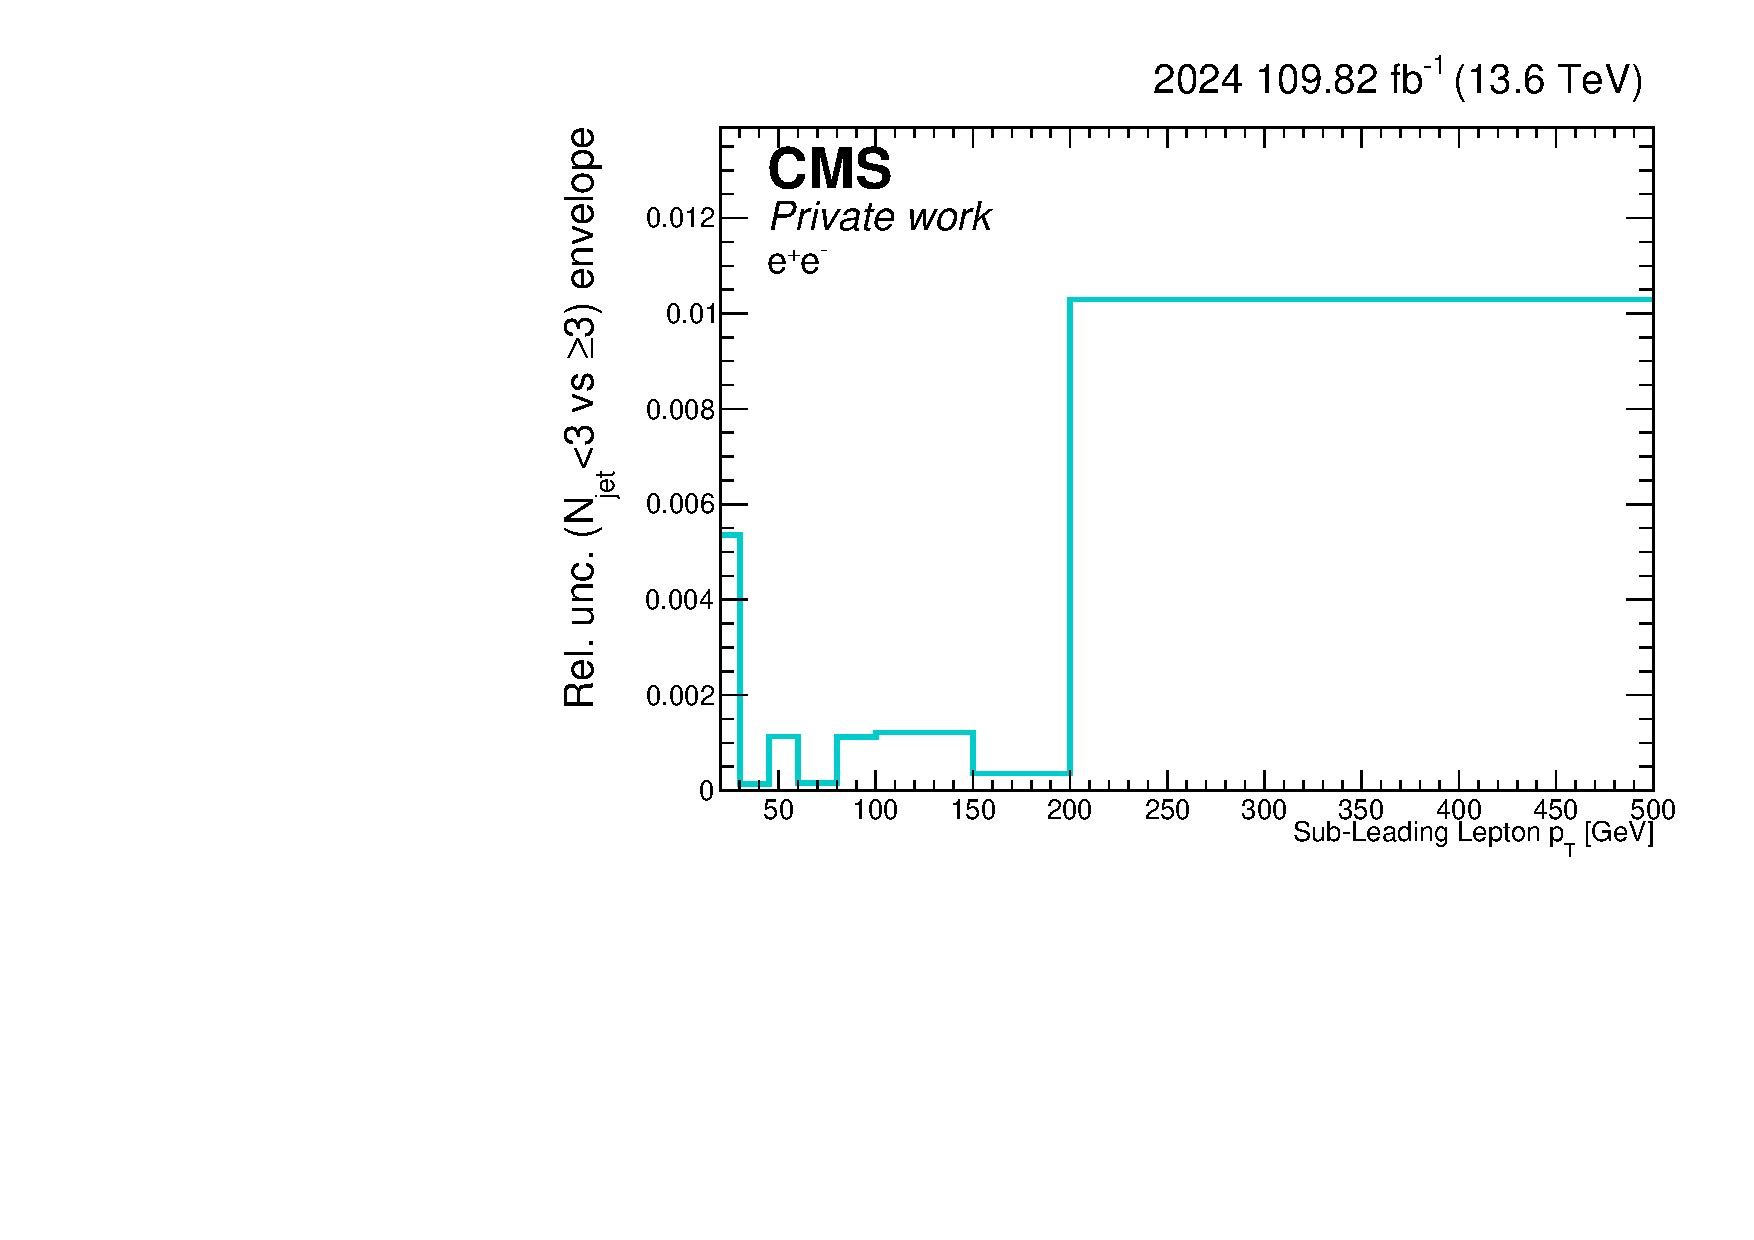
\includegraphics[width=0.48\linewidth]{figures/2024/ElEl/Jet_Topology_Uncertainty/TopoJetUnc_Lep2pt.pdf}
\caption{Jet Topology Uncertainty diagnostics in the $ee$ channel versus leading and subleading lepton momentum. Curves are reproduced with the production definitions; their exact numerical prescription requires confirmation.}\label{fig:study-ElEl-TopoJetUnc}
\end{figure}
\begin{figure}[htbp]\centering
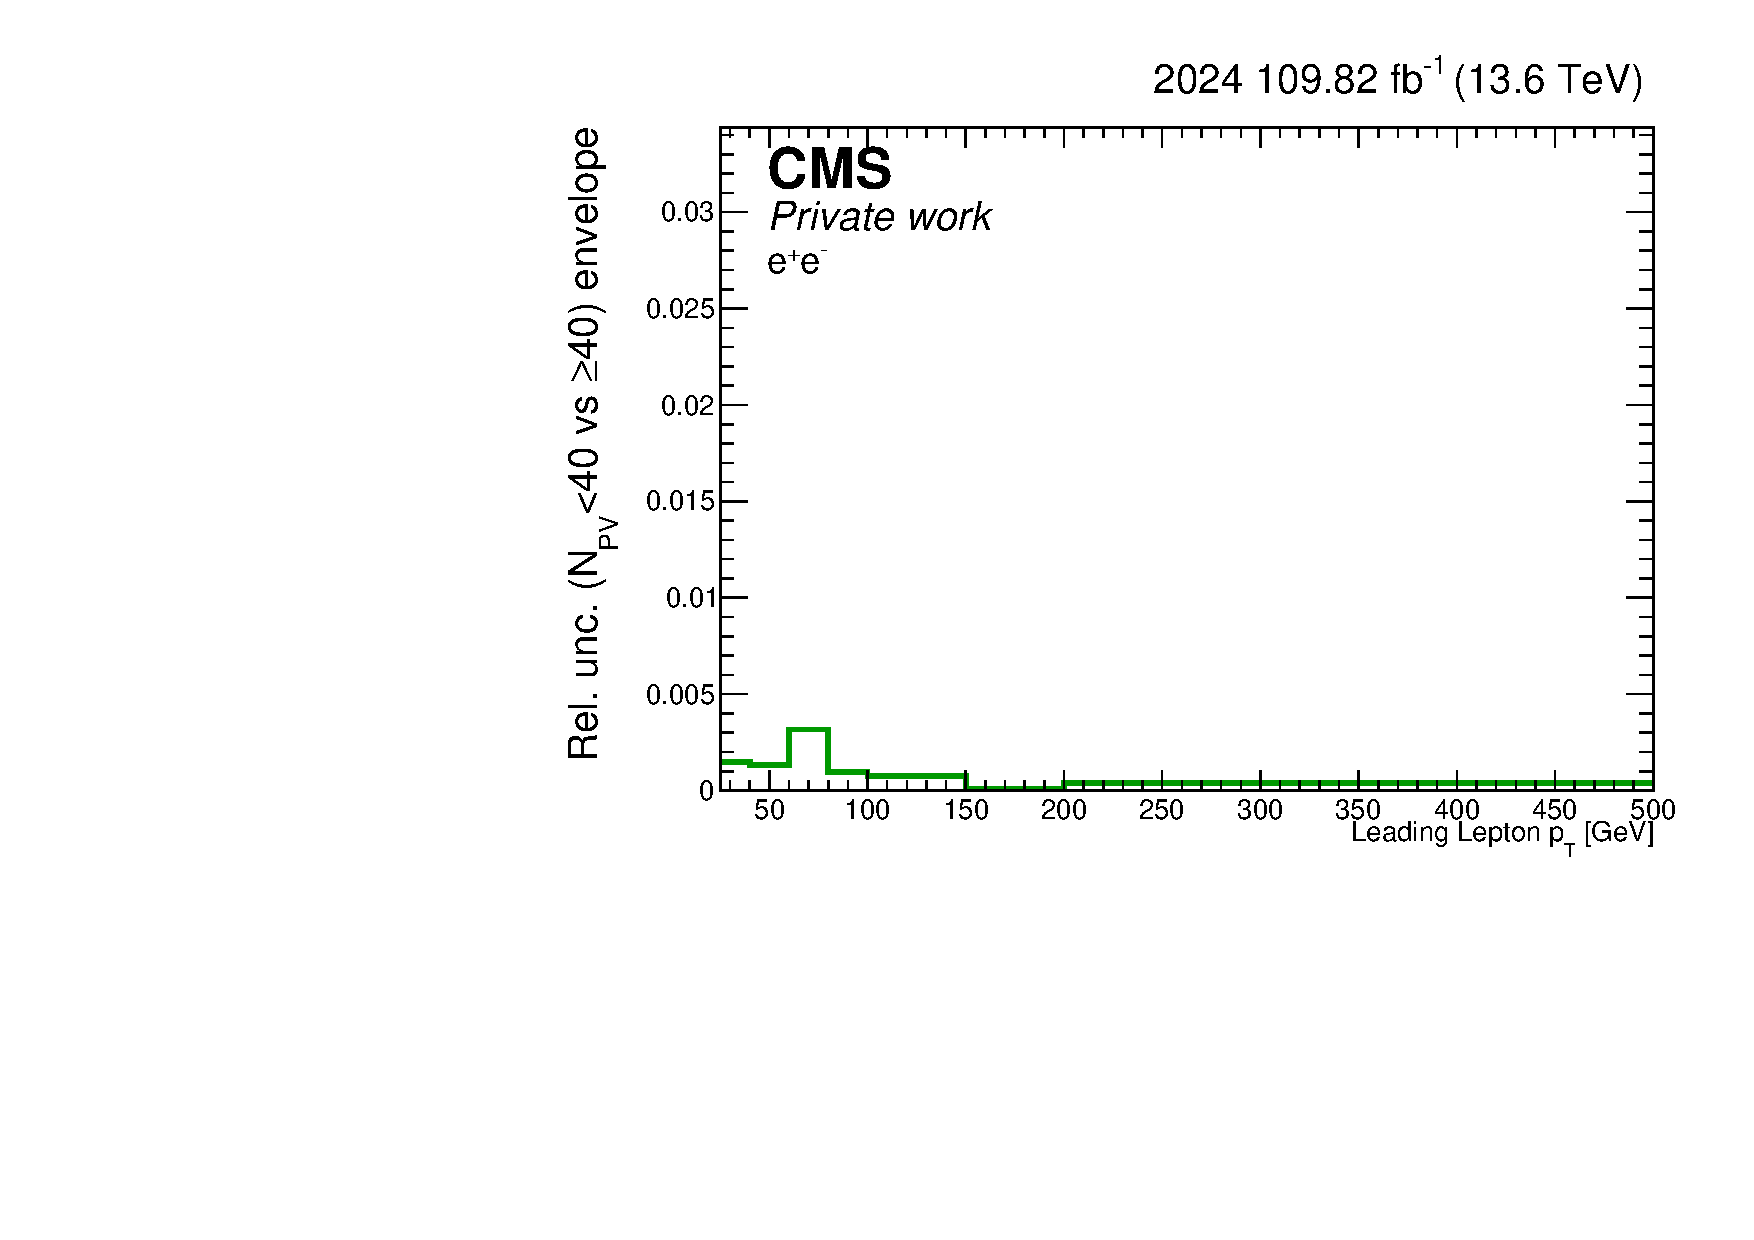
\includegraphics[width=0.48\linewidth]{figures/2024/ElEl/PV_Topology_Uncertainty/TopoPVUnc_Lep1pt.pdf}
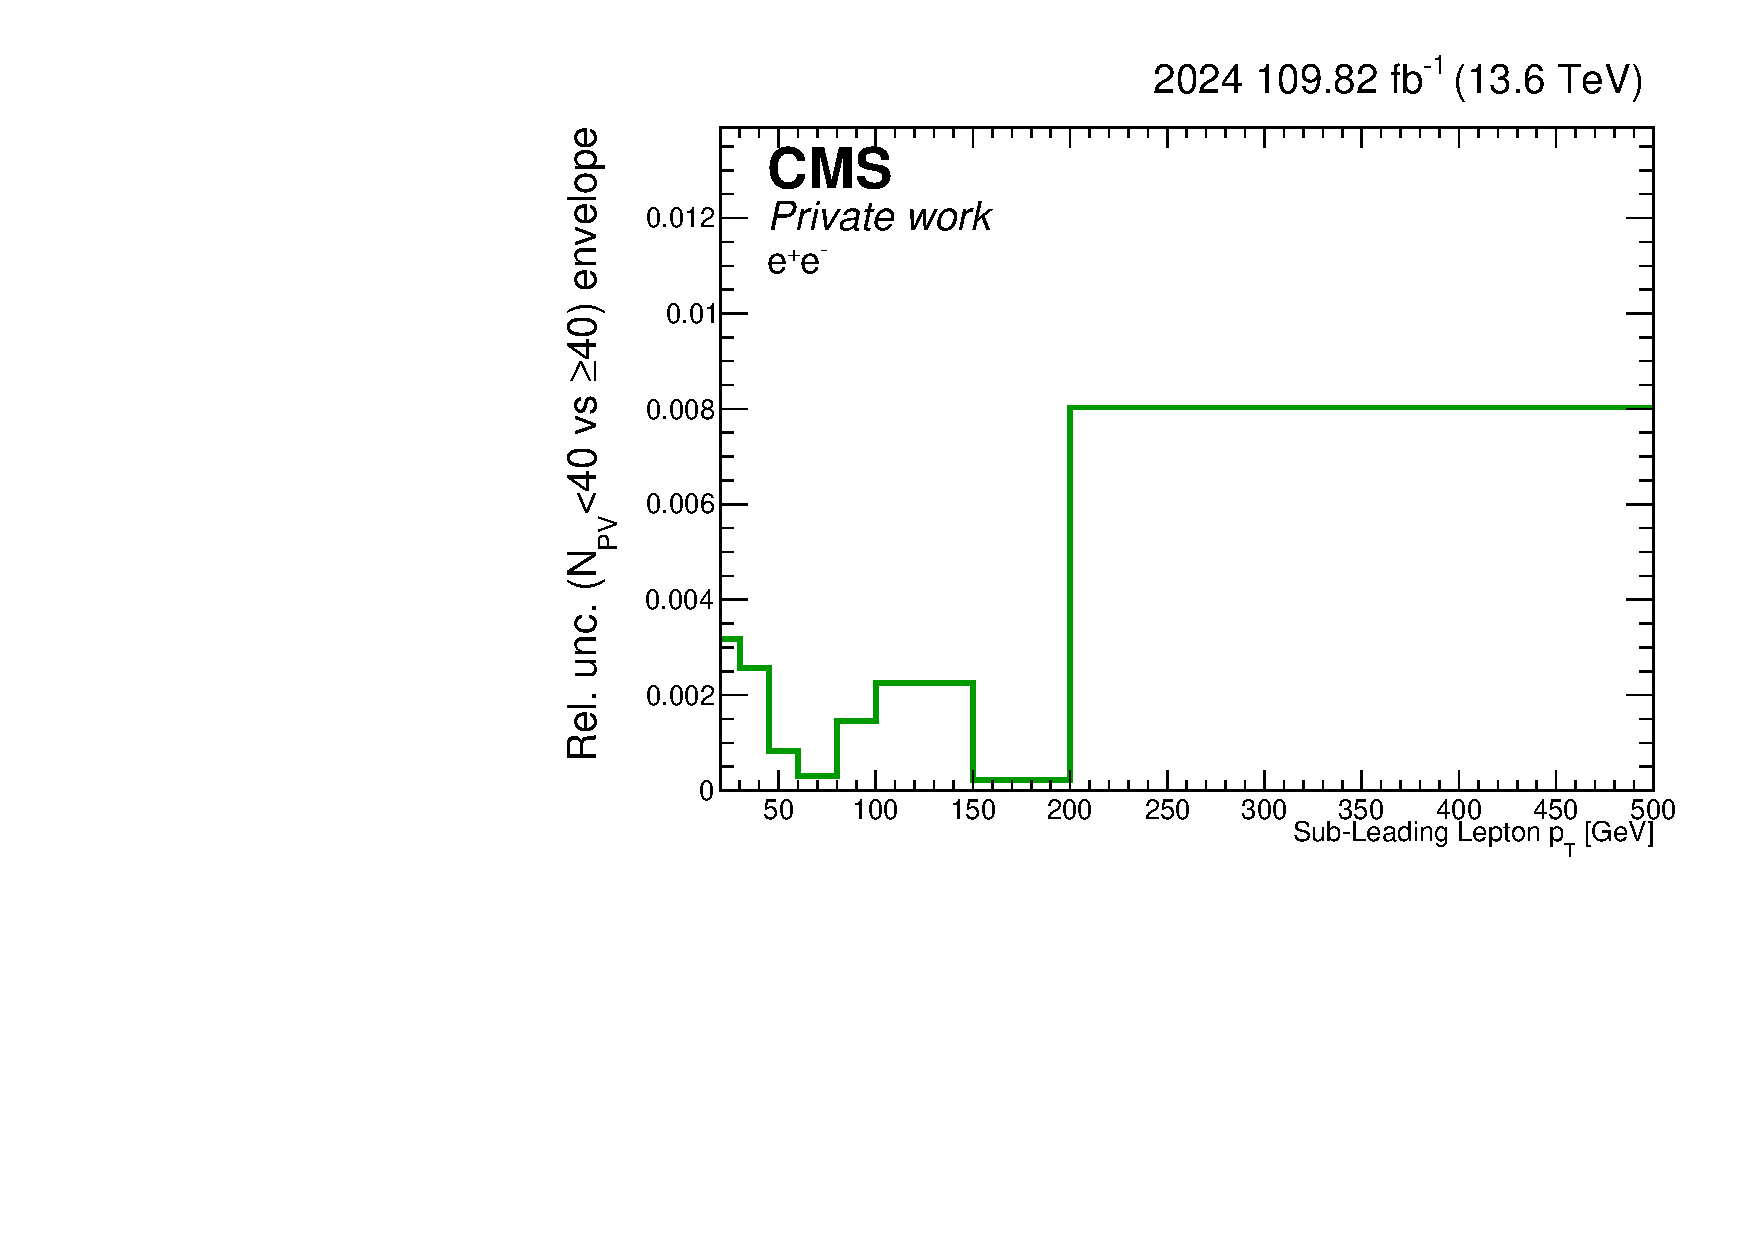
\includegraphics[width=0.48\linewidth]{figures/2024/ElEl/PV_Topology_Uncertainty/TopoPVUnc_Lep2pt.pdf}
\caption{PV Topology Uncertainty diagnostics in the $ee$ channel versus leading and subleading lepton momentum. Curves are reproduced with the production definitions; their exact numerical prescription requires confirmation.}\label{fig:study-ElEl-TopoPVUnc}
\end{figure}
\begin{figure}[htbp]\centering
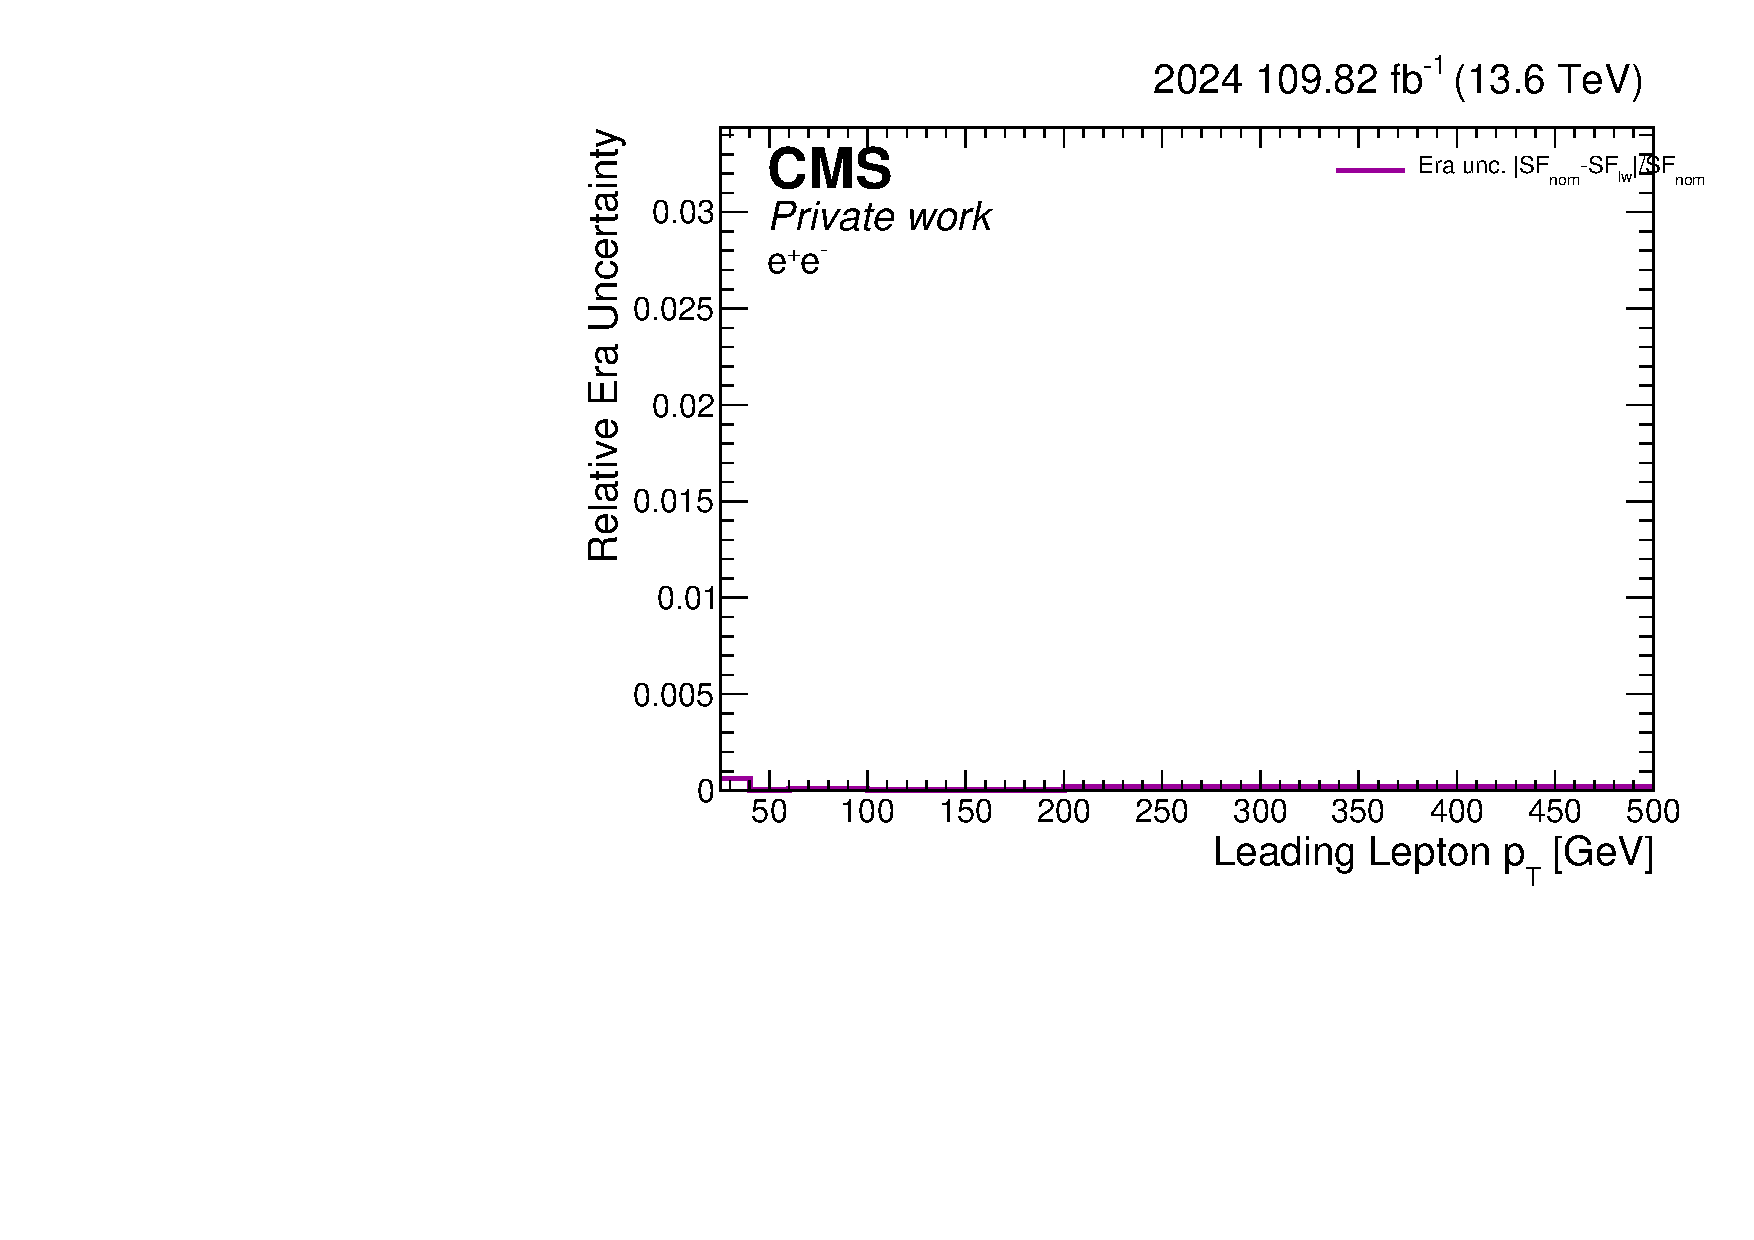
\includegraphics[width=0.48\linewidth]{figures/2024/ElEl/Era_Uncertainty/EraUnc_Lep1pt.pdf}
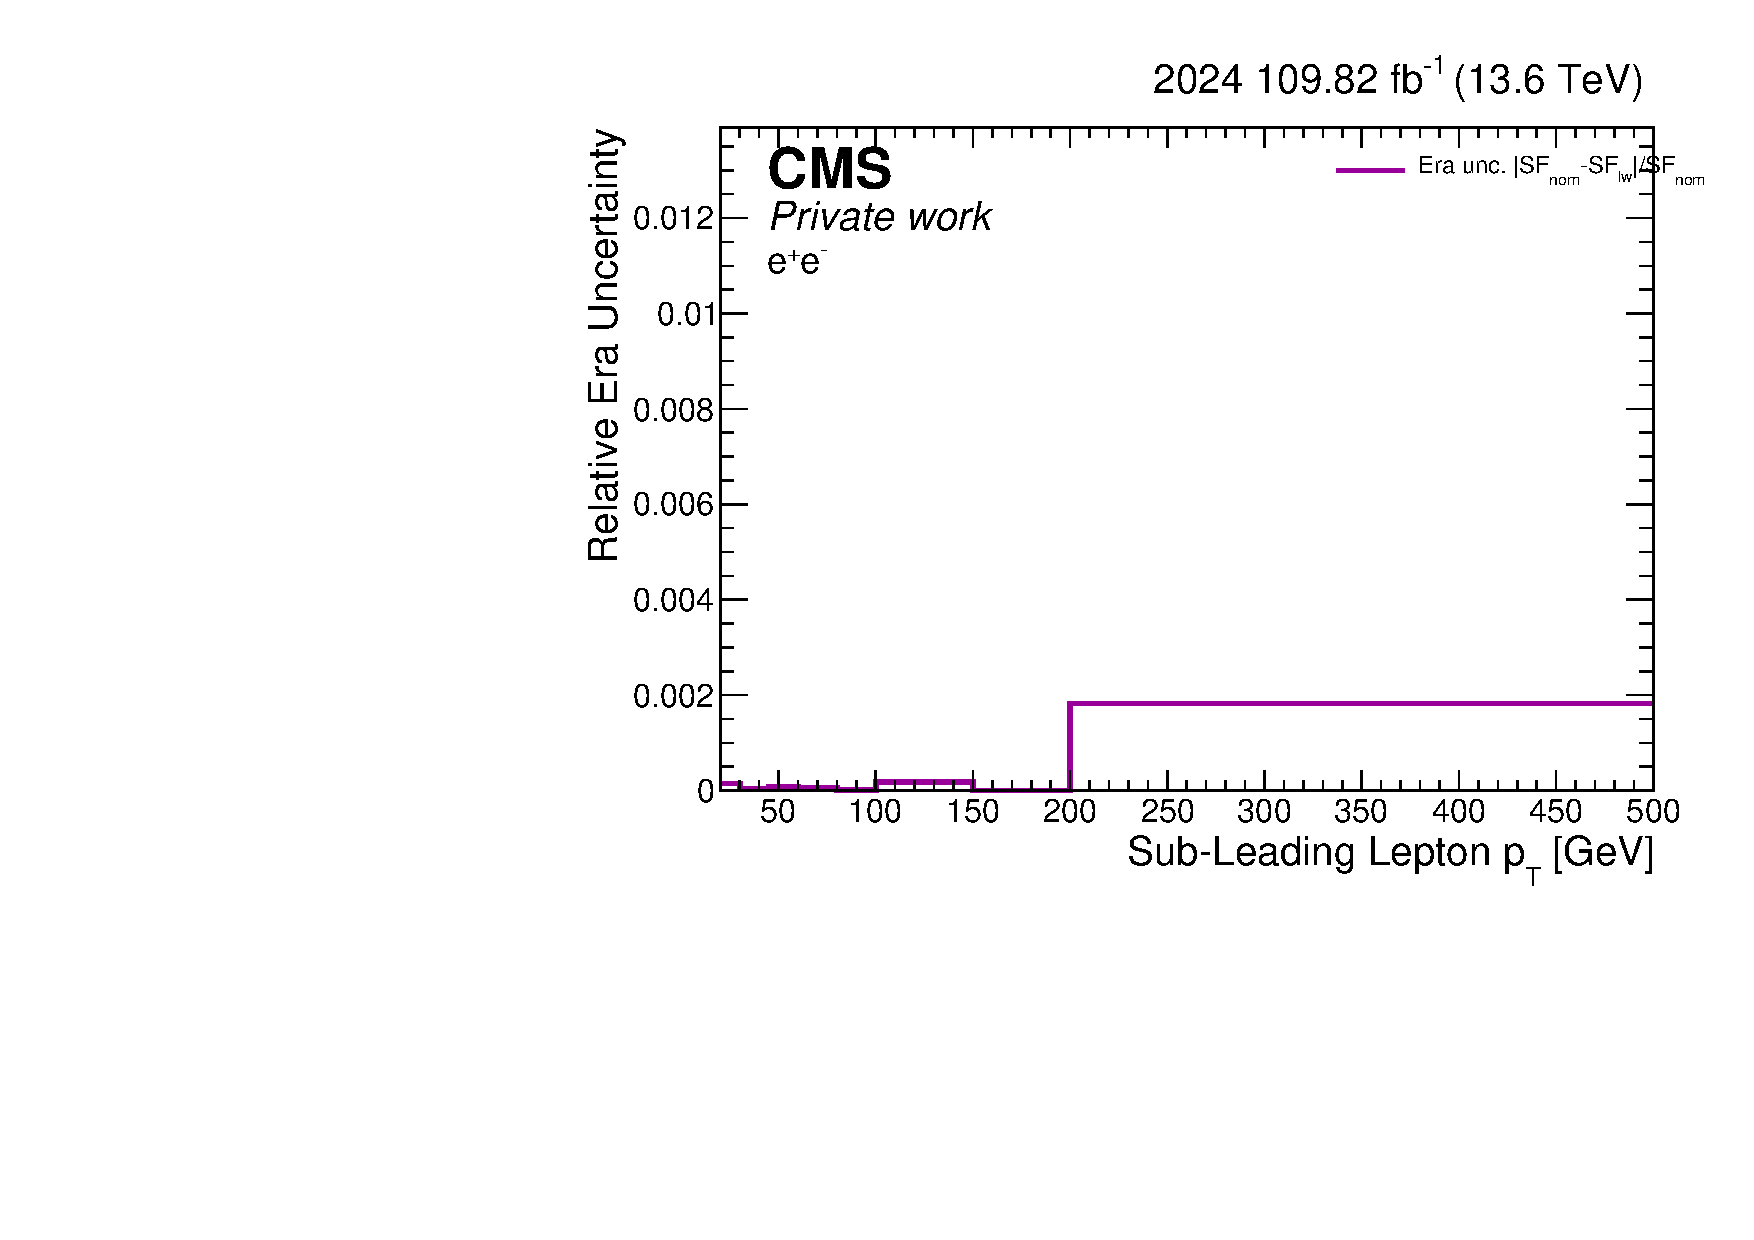
\includegraphics[width=0.48\linewidth]{figures/2024/ElEl/Era_Uncertainty/EraUnc_Lep2pt.pdf}
\caption{Era Uncertainty diagnostics in the $ee$ channel versus leading and subleading lepton momentum. Curves are reproduced with the production definitions; their exact numerical prescription requires confirmation.}\label{fig:study-ElEl-EraUnc}
\end{figure}
\begin{figure}[htbp]\centering
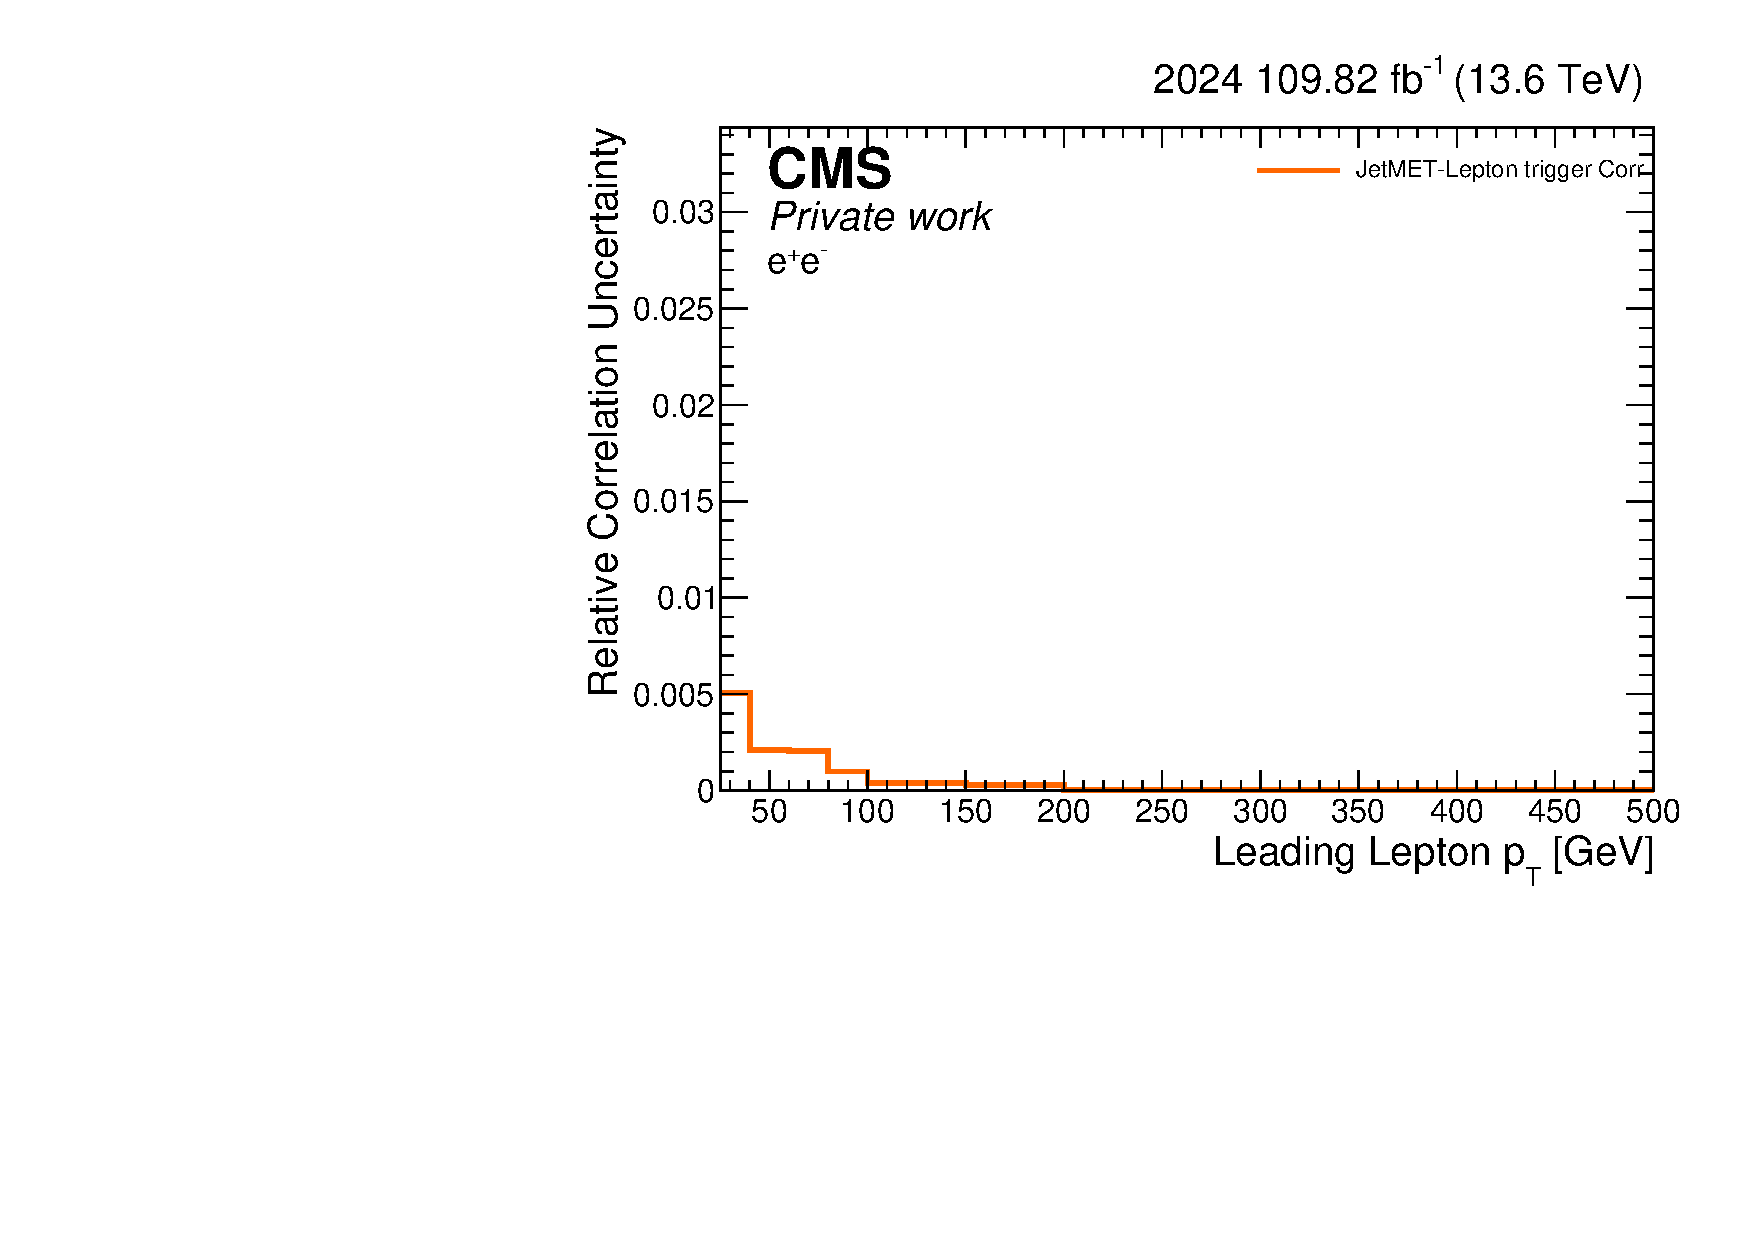
\includegraphics[width=0.48\linewidth]{figures/2024/ElEl/Correlation_Uncertainty/CorrUnc_Lep1pt.pdf}
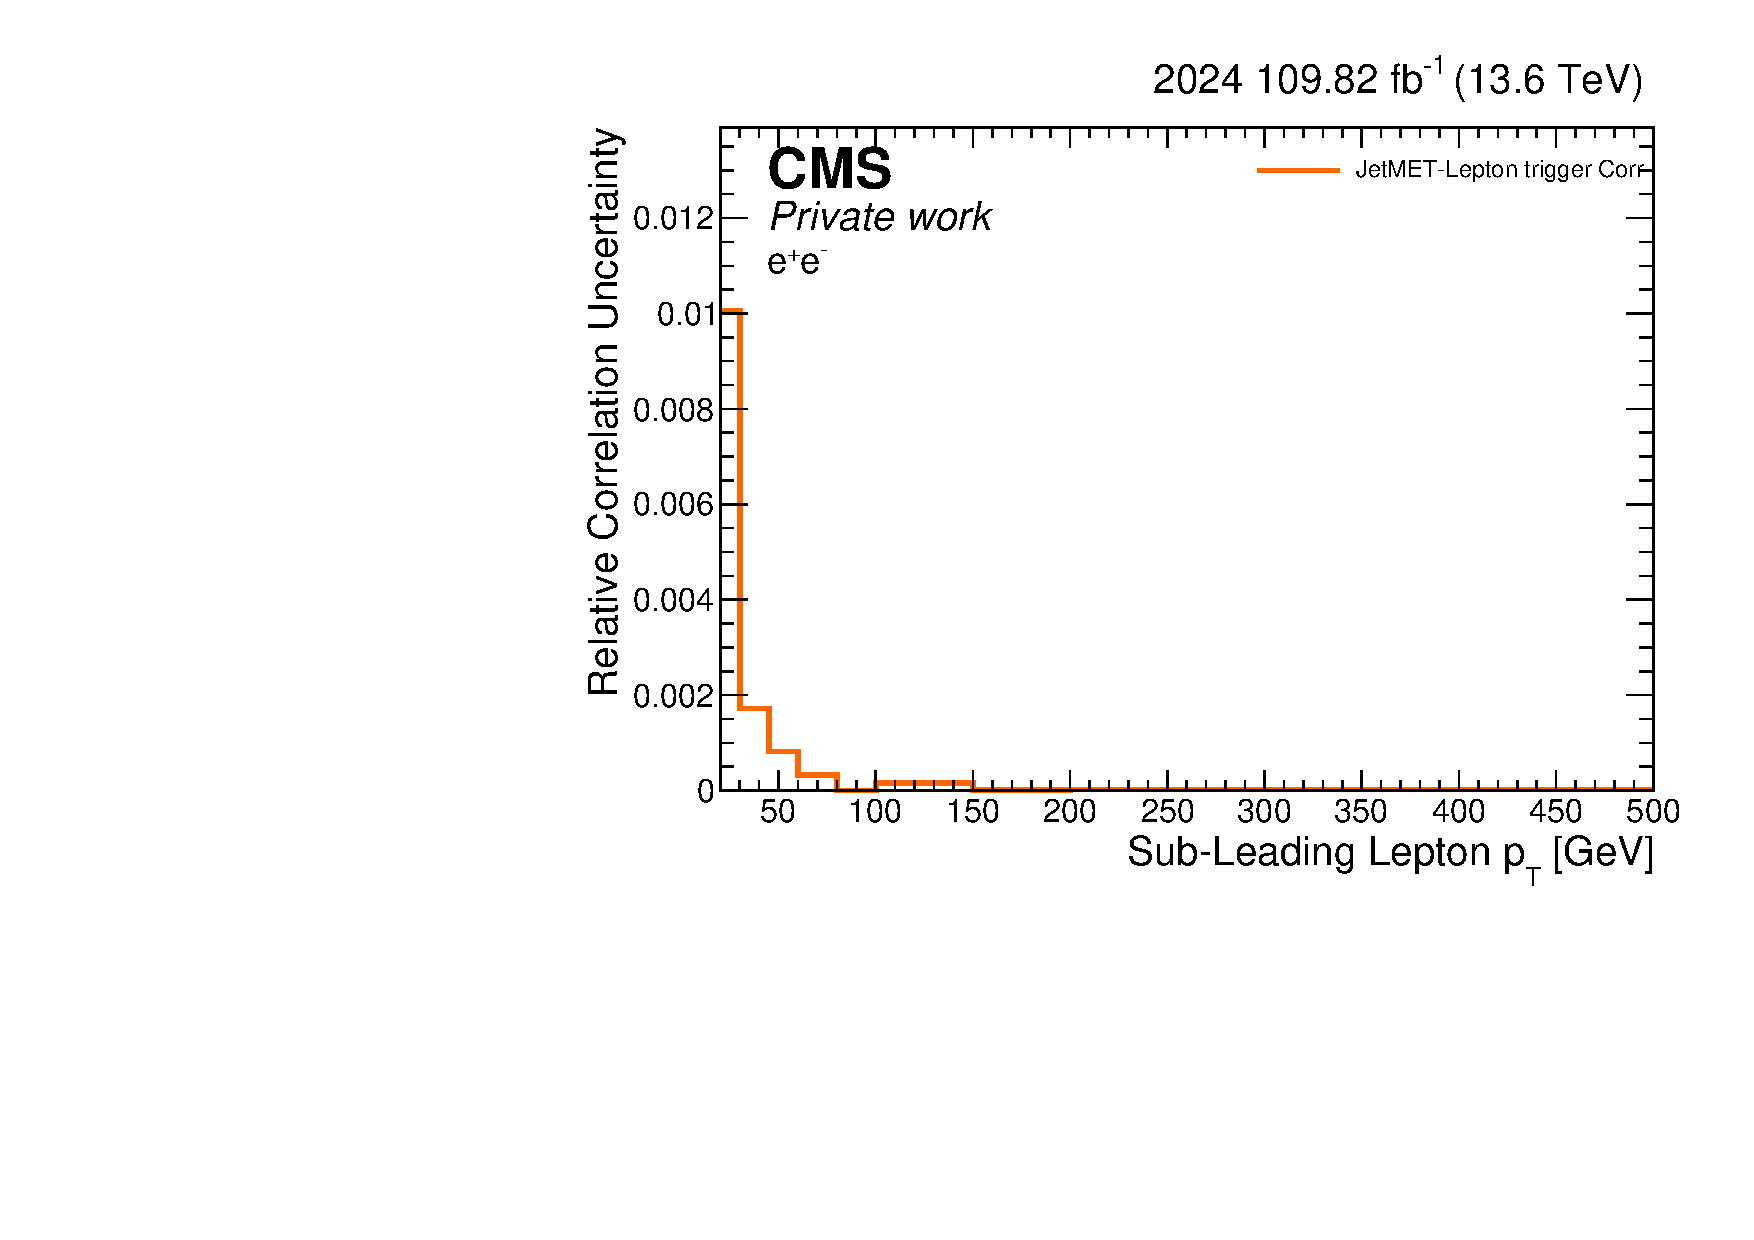
\includegraphics[width=0.48\linewidth]{figures/2024/ElEl/Correlation_Uncertainty/CorrUnc_Lep2pt.pdf}
\caption{Correlation Uncertainty diagnostics in the $ee$ channel versus leading and subleading lepton momentum. Curves are reproduced with the production definitions; their exact numerical prescription requires confirmation.}\label{fig:study-ElEl-CorrUnc}
\end{figure}
\begin{figure}[htbp]\centering
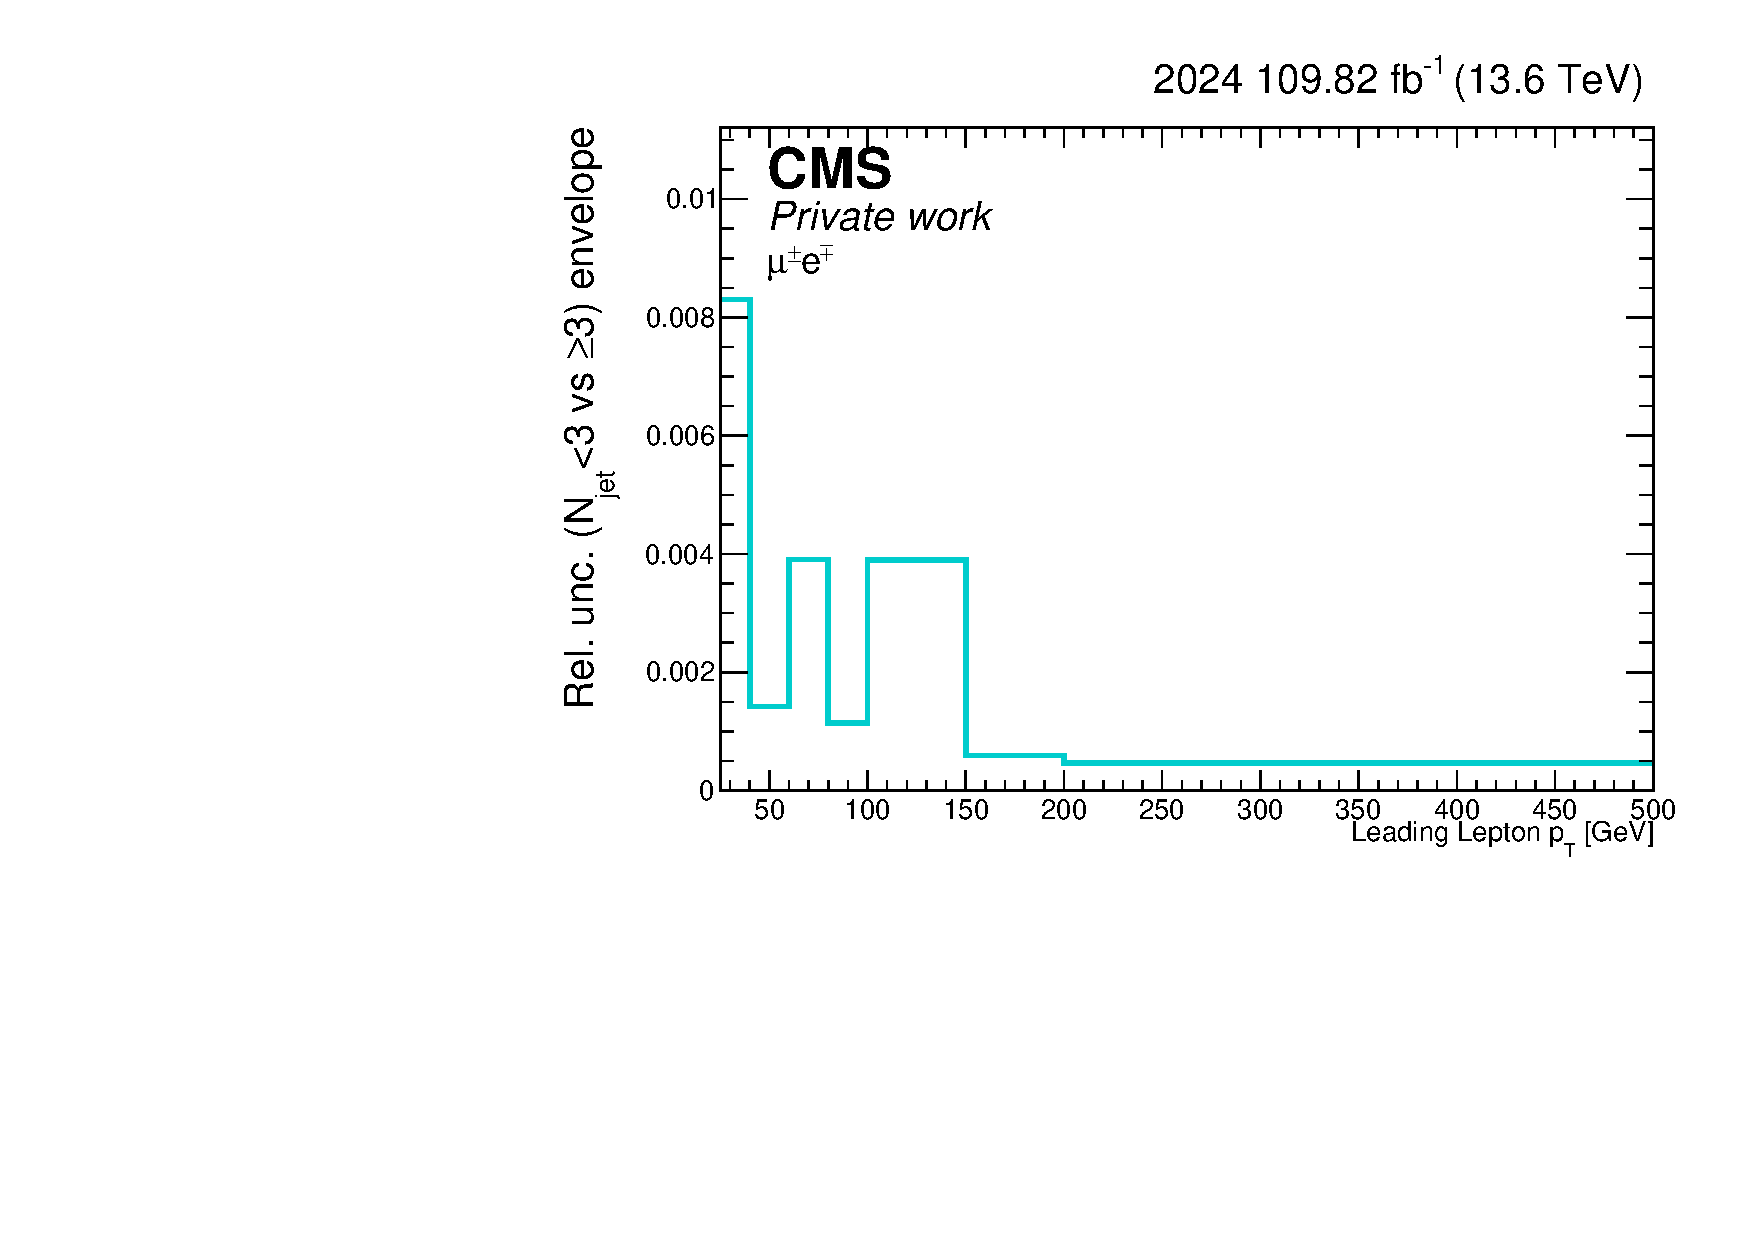
\includegraphics[width=0.48\linewidth]{figures/2024/MuEl/Jet_Topology_Uncertainty/TopoJetUnc_Lep1pt.pdf}
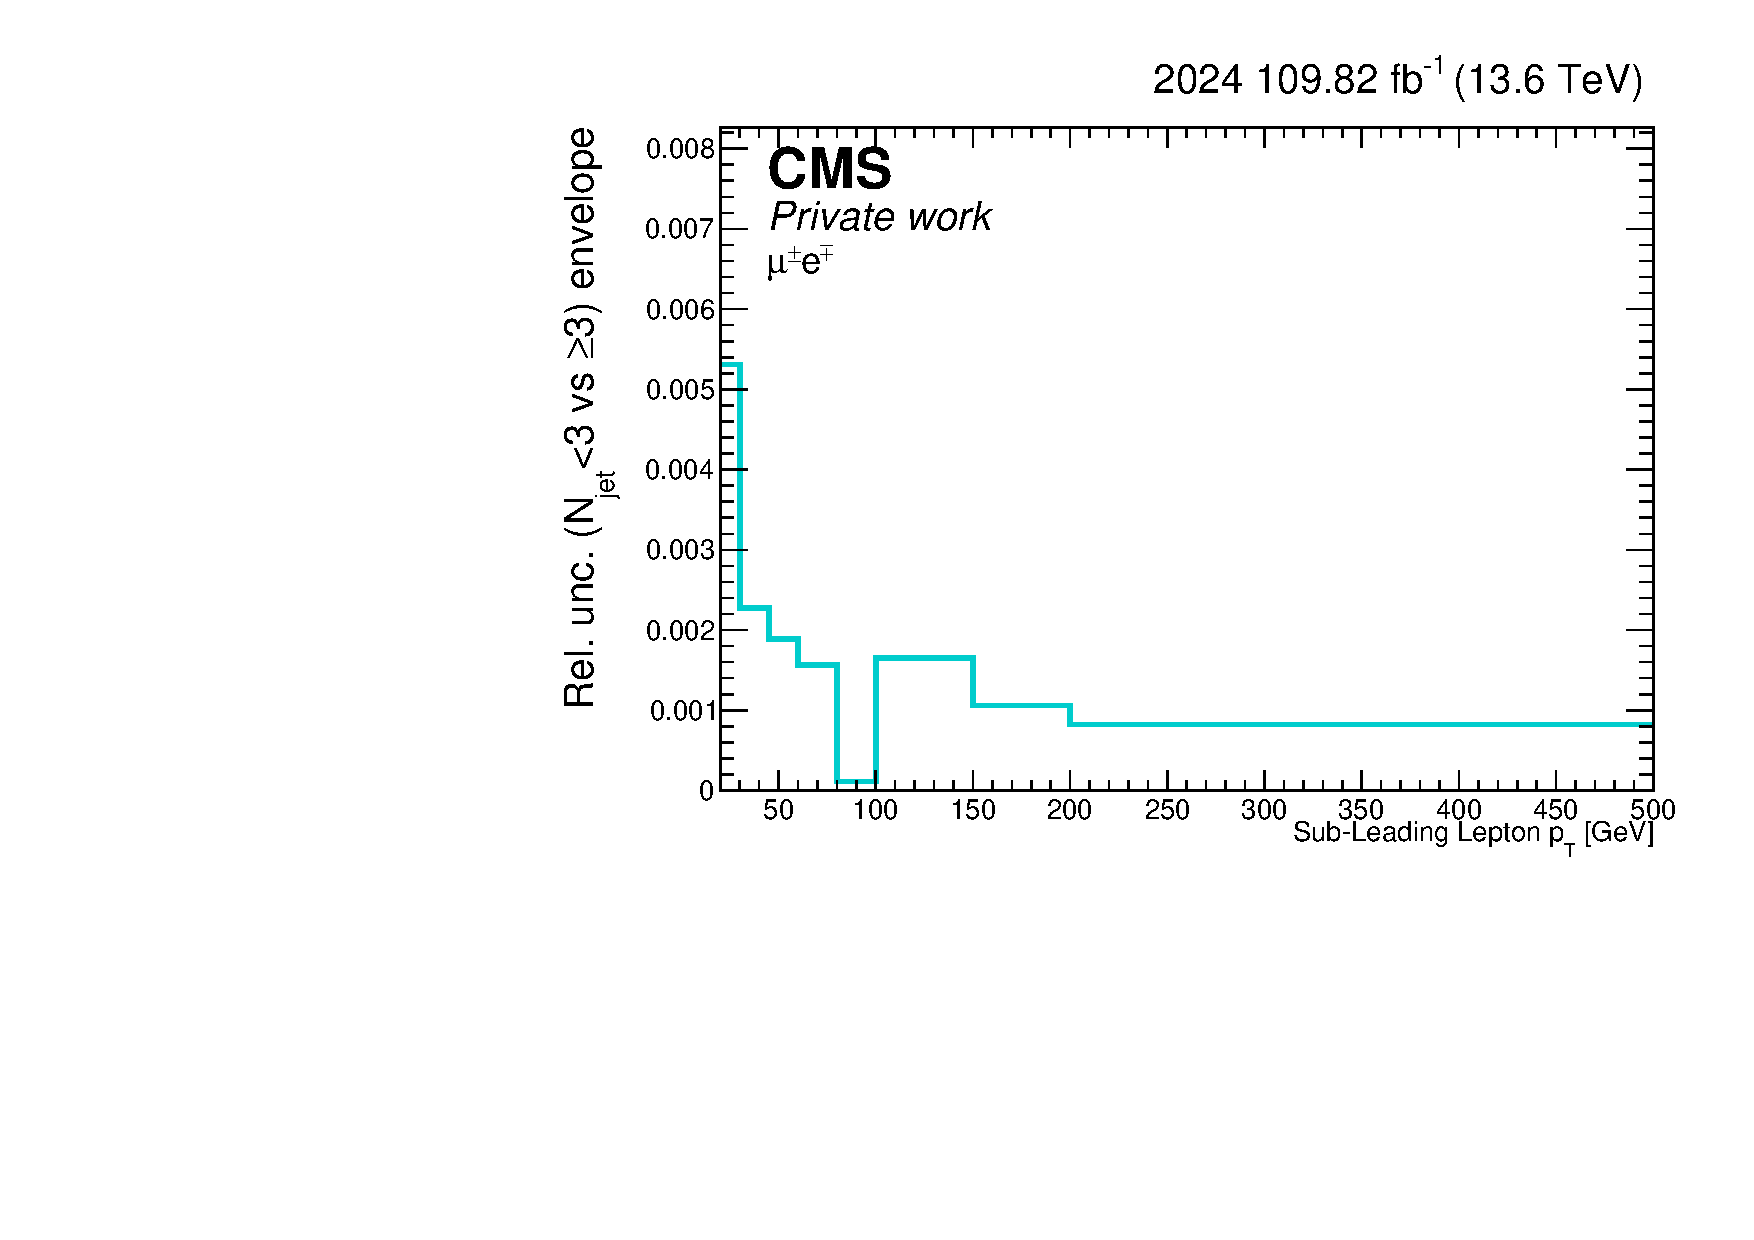
\includegraphics[width=0.48\linewidth]{figures/2024/MuEl/Jet_Topology_Uncertainty/TopoJetUnc_Lep2pt.pdf}
\caption{Jet Topology Uncertainty diagnostics in the $e\mu$ channel versus leading and subleading lepton momentum. Curves are reproduced with the production definitions; their exact numerical prescription requires confirmation.}\label{fig:study-MuEl-TopoJetUnc}
\end{figure}
\begin{figure}[htbp]\centering
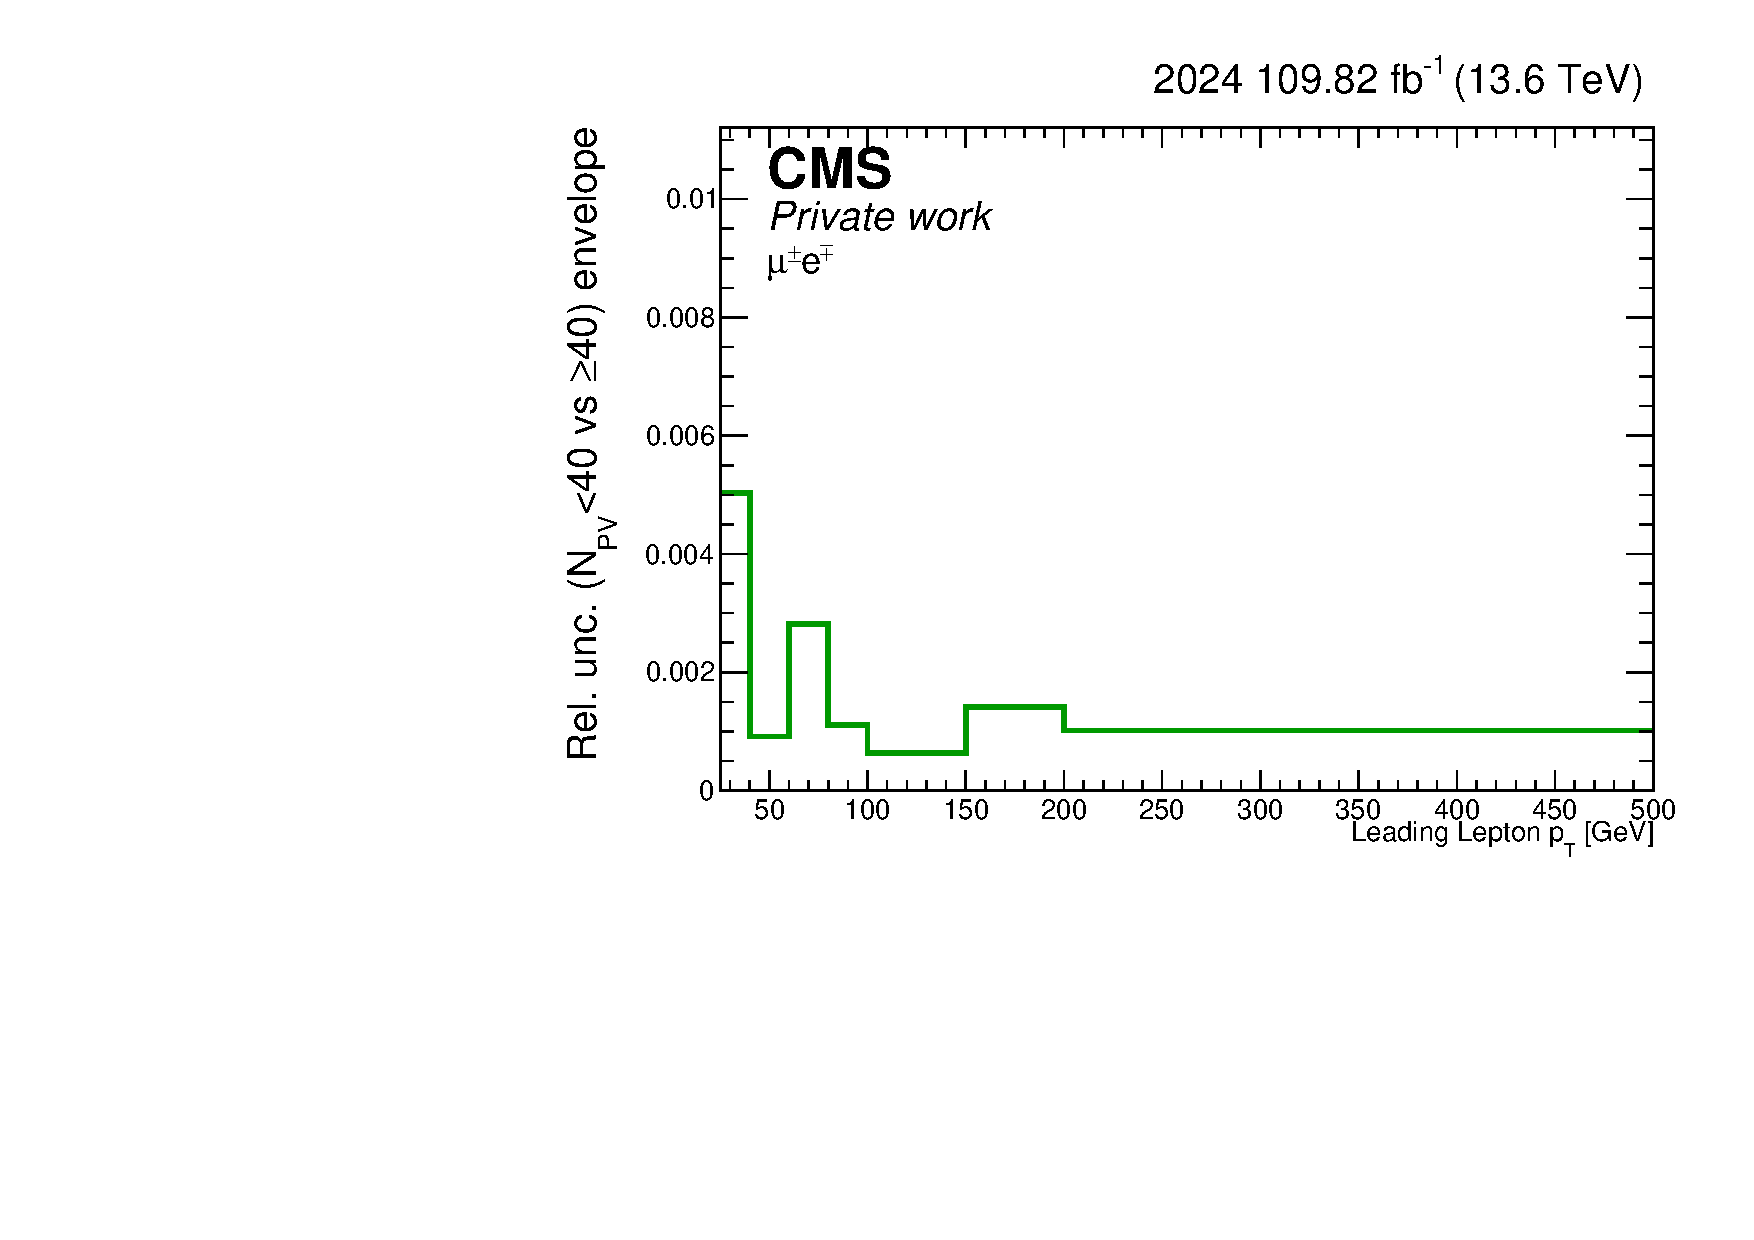
\includegraphics[width=0.48\linewidth]{figures/2024/MuEl/PV_Topology_Uncertainty/TopoPVUnc_Lep1pt.pdf}
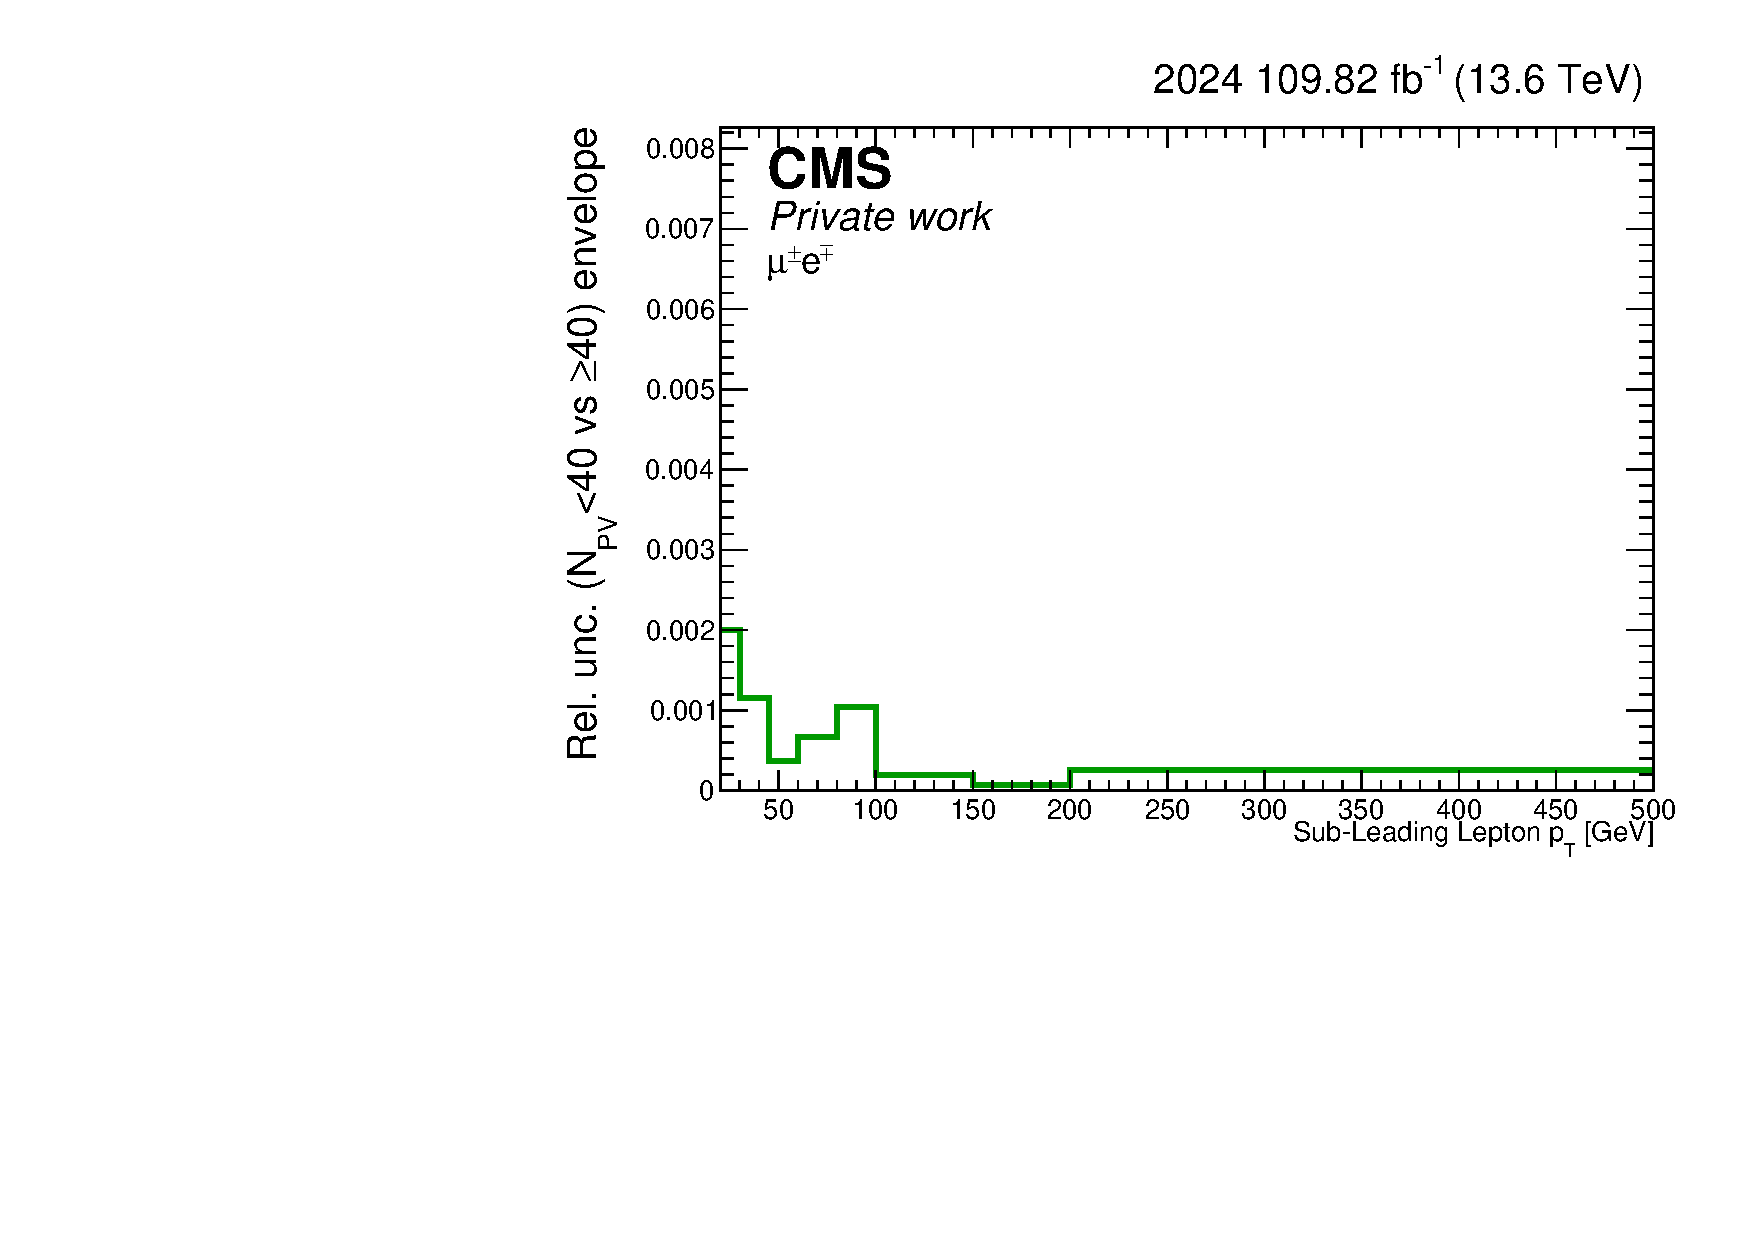
\includegraphics[width=0.48\linewidth]{figures/2024/MuEl/PV_Topology_Uncertainty/TopoPVUnc_Lep2pt.pdf}
\caption{PV Topology Uncertainty diagnostics in the $e\mu$ channel versus leading and subleading lepton momentum. Curves are reproduced with the production definitions; their exact numerical prescription requires confirmation.}\label{fig:study-MuEl-TopoPVUnc}
\end{figure}
\begin{figure}[htbp]\centering
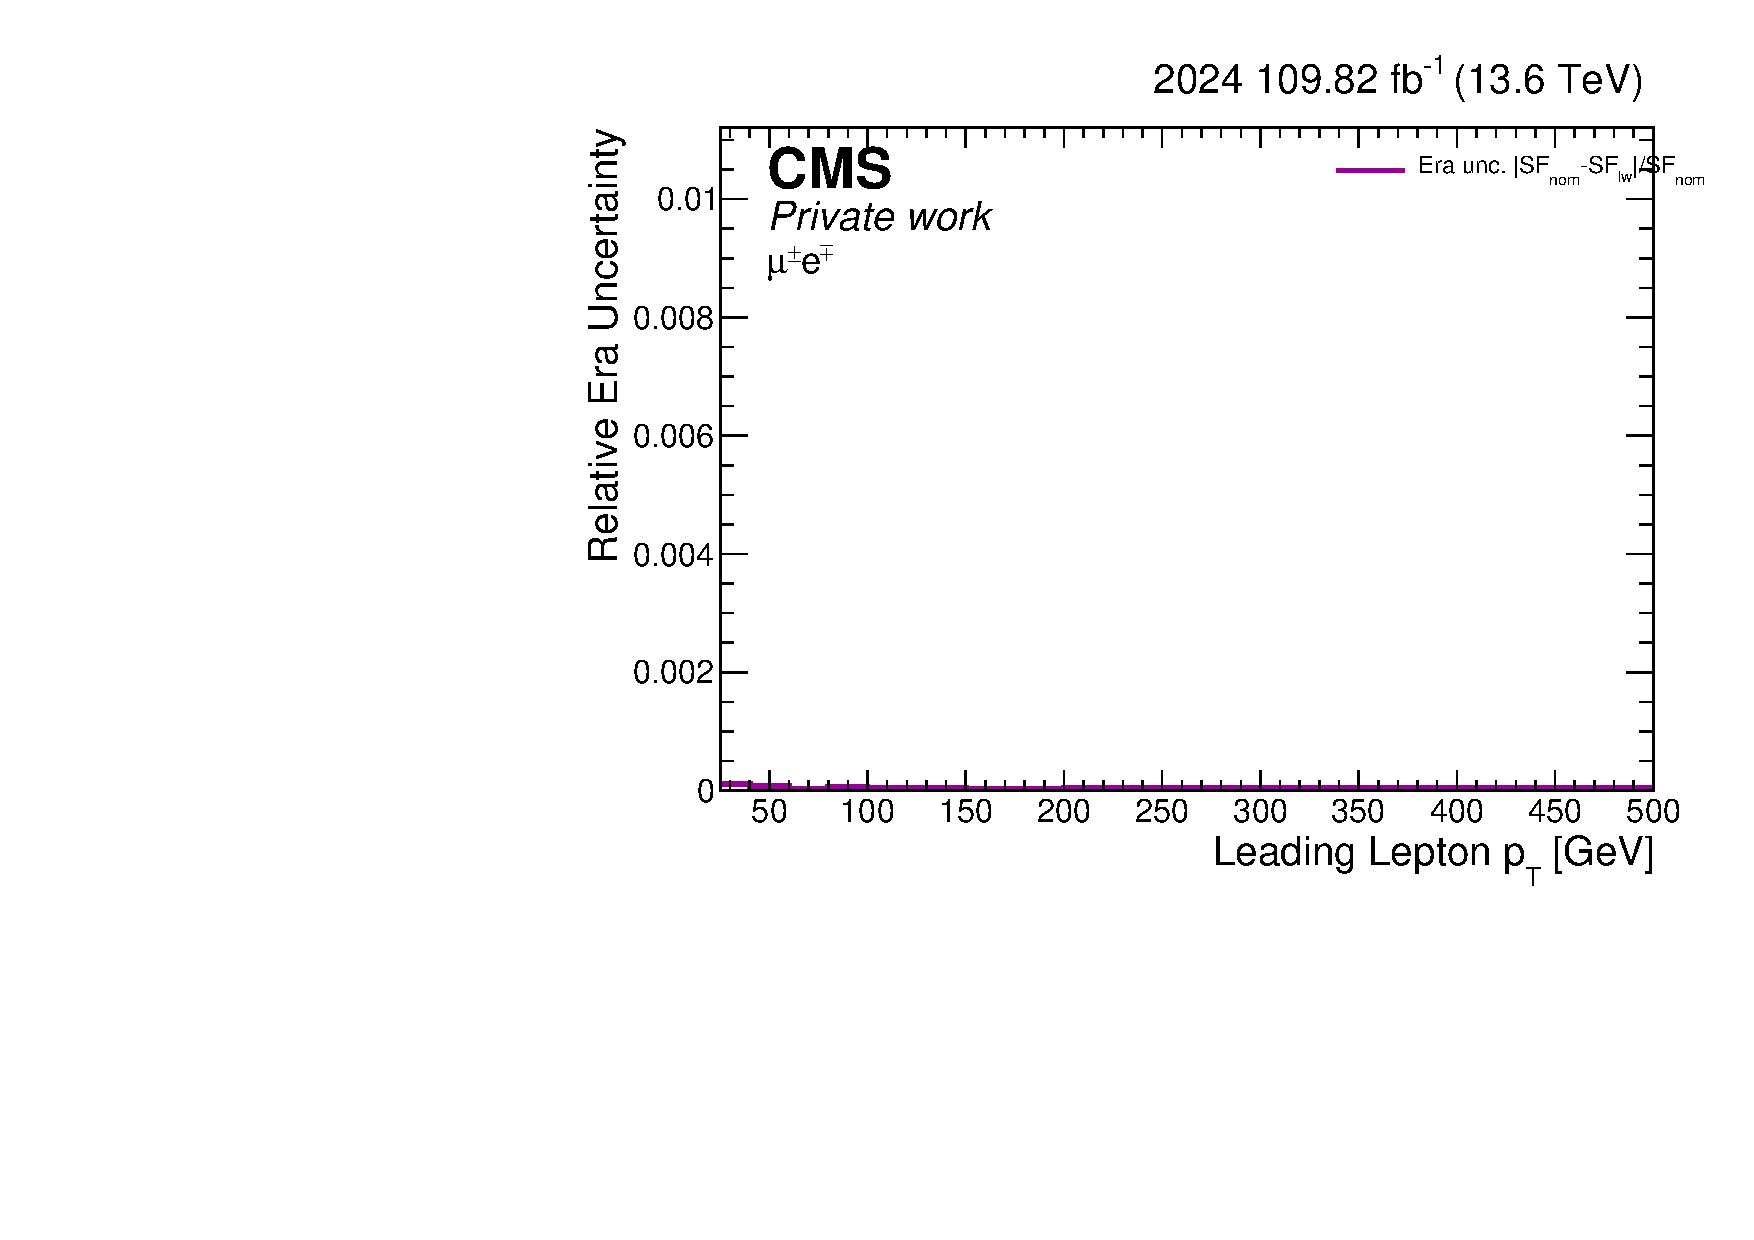
\includegraphics[width=0.48\linewidth]{figures/2024/MuEl/Era_Uncertainty/EraUnc_Lep1pt.pdf}
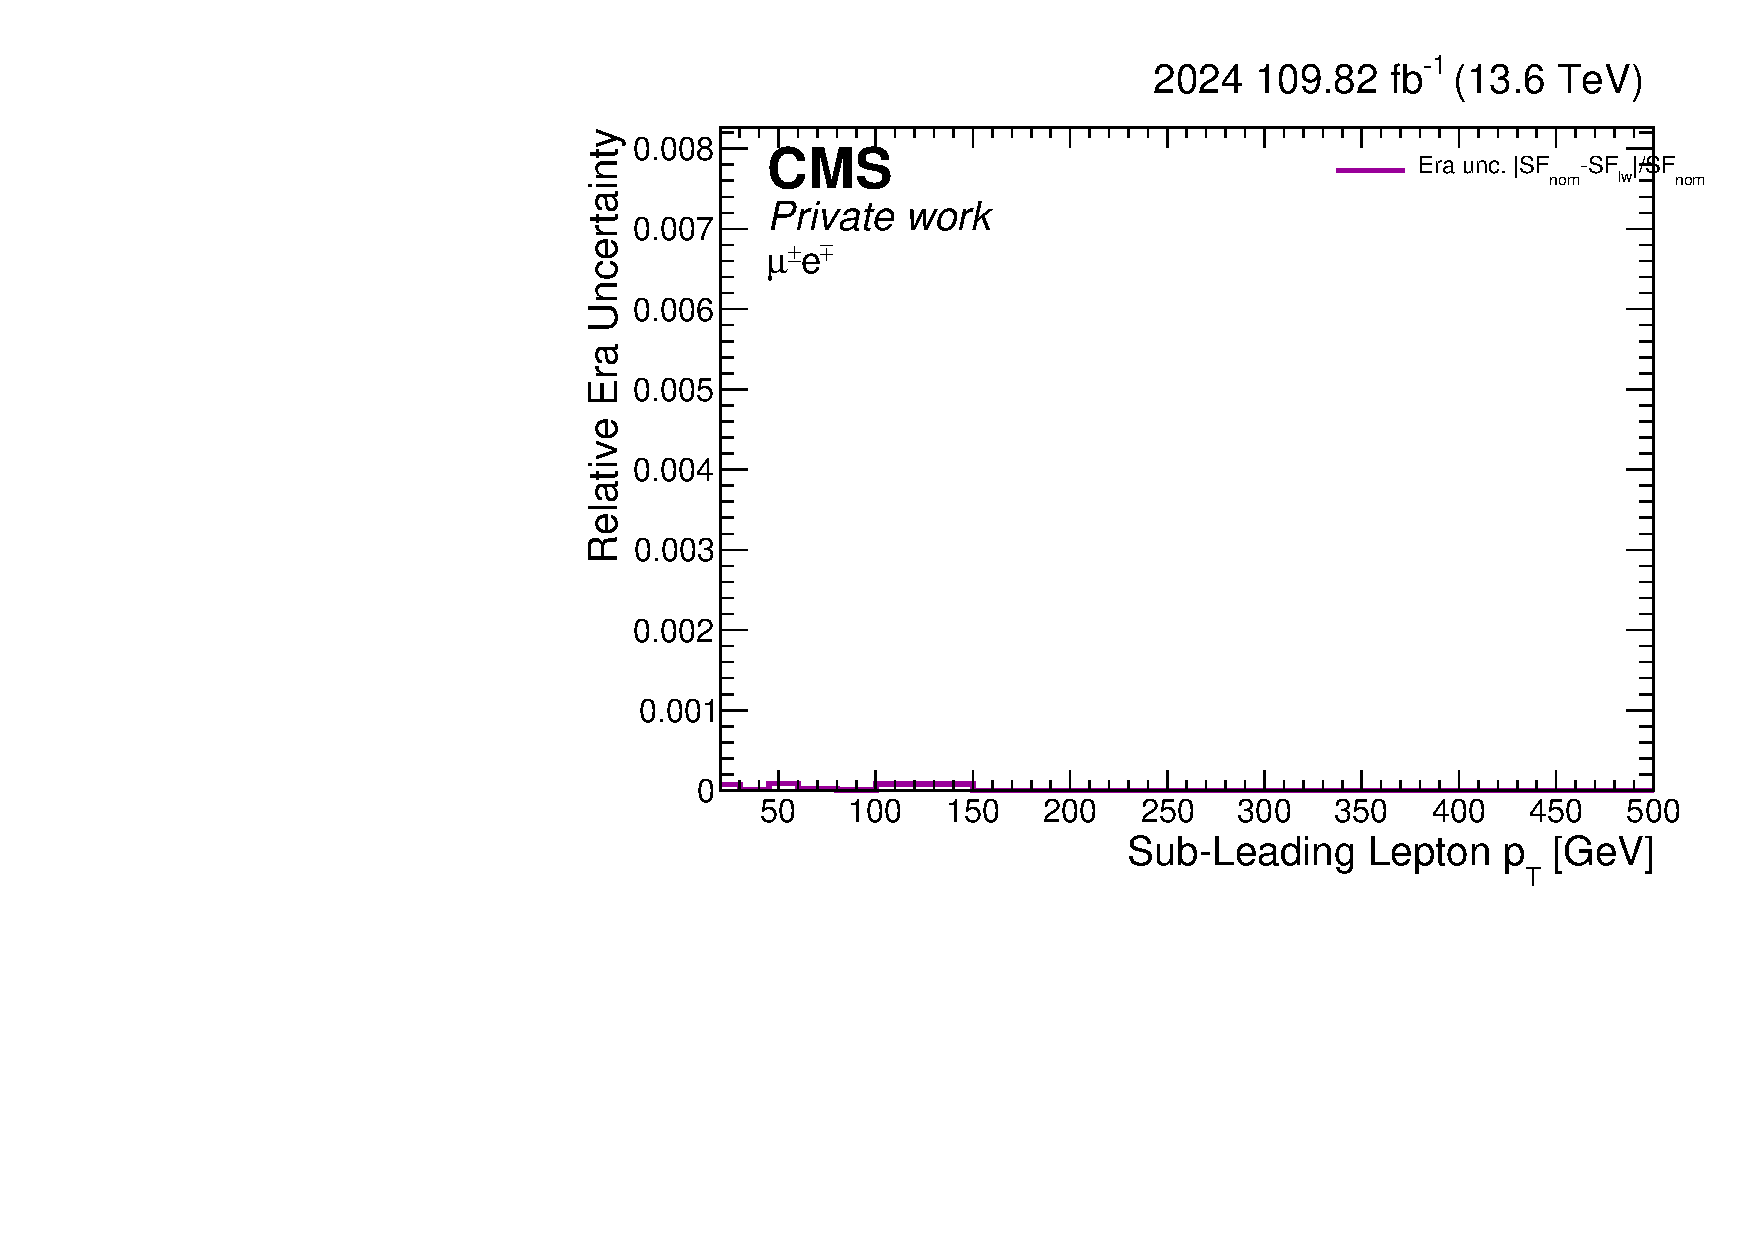
\includegraphics[width=0.48\linewidth]{figures/2024/MuEl/Era_Uncertainty/EraUnc_Lep2pt.pdf}
\caption{Era Uncertainty diagnostics in the $e\mu$ channel versus leading and subleading lepton momentum. Curves are reproduced with the production definitions; their exact numerical prescription requires confirmation.}\label{fig:study-MuEl-EraUnc}
\end{figure}
\begin{figure}[htbp]\centering
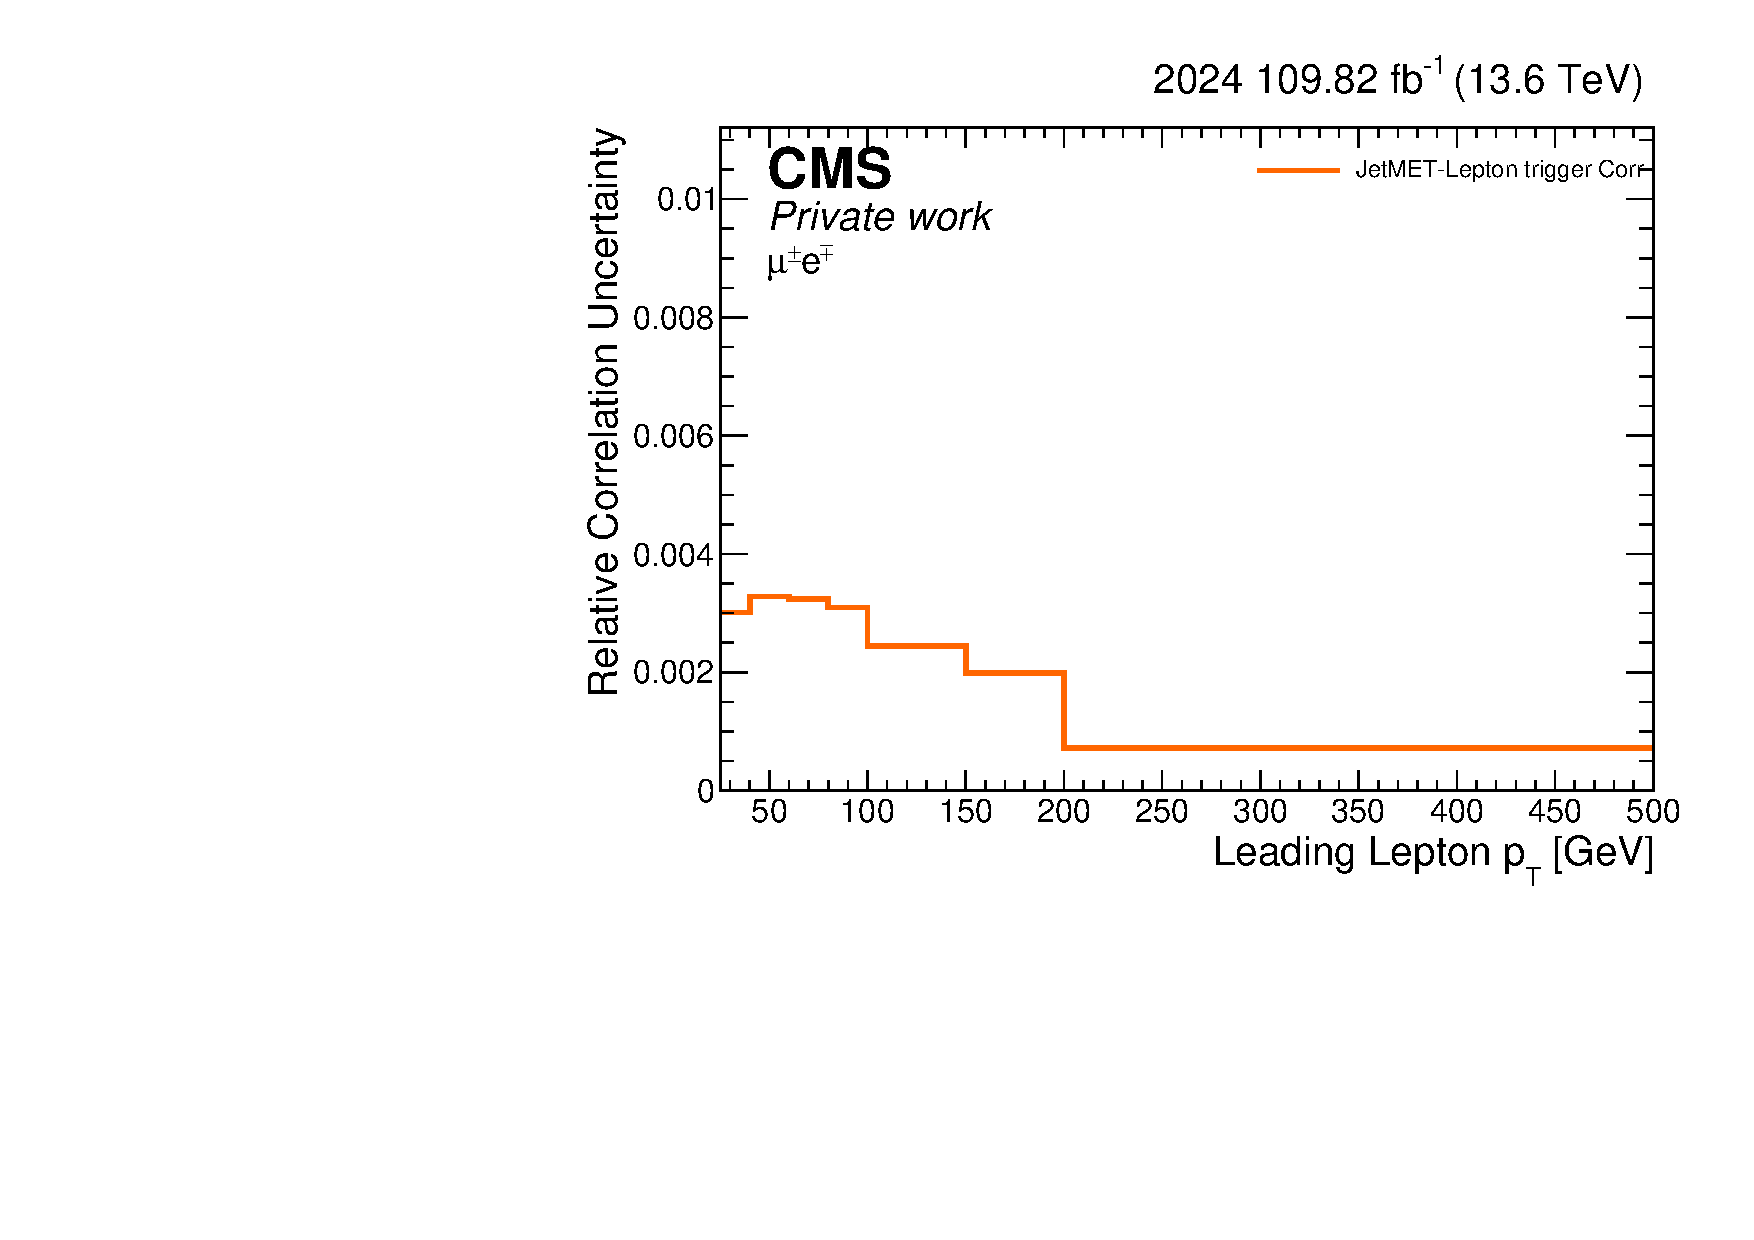
\includegraphics[width=0.48\linewidth]{figures/2024/MuEl/Correlation_Uncertainty/CorrUnc_Lep1pt.pdf}
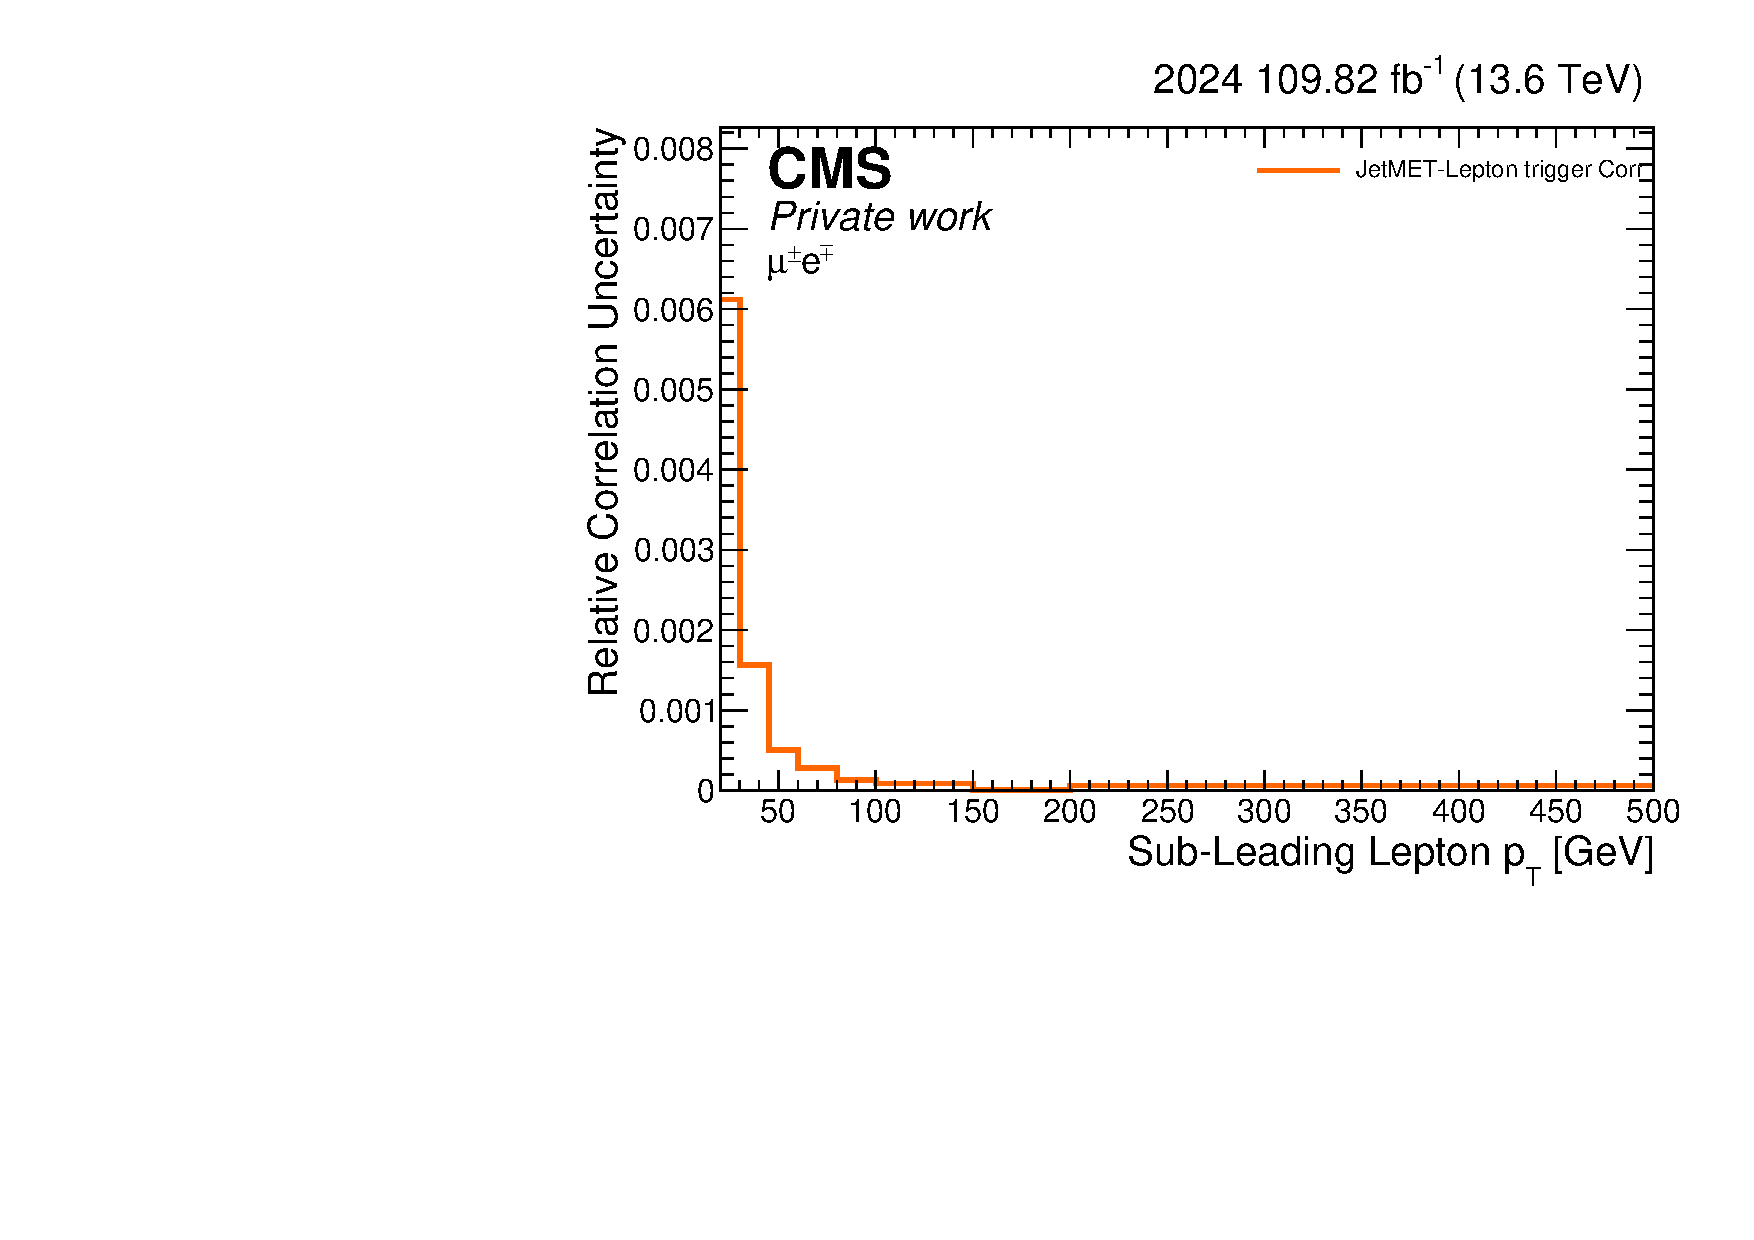
\includegraphics[width=0.48\linewidth]{figures/2024/MuEl/Correlation_Uncertainty/CorrUnc_Lep2pt.pdf}
\caption{Correlation Uncertainty diagnostics in the $e\mu$ channel versus leading and subleading lepton momentum. Curves are reproduced with the production definitions; their exact numerical prescription requires confirmation.}\label{fig:study-MuEl-CorrUnc}
\end{figure}
\begin{figure}[htbp]\centering
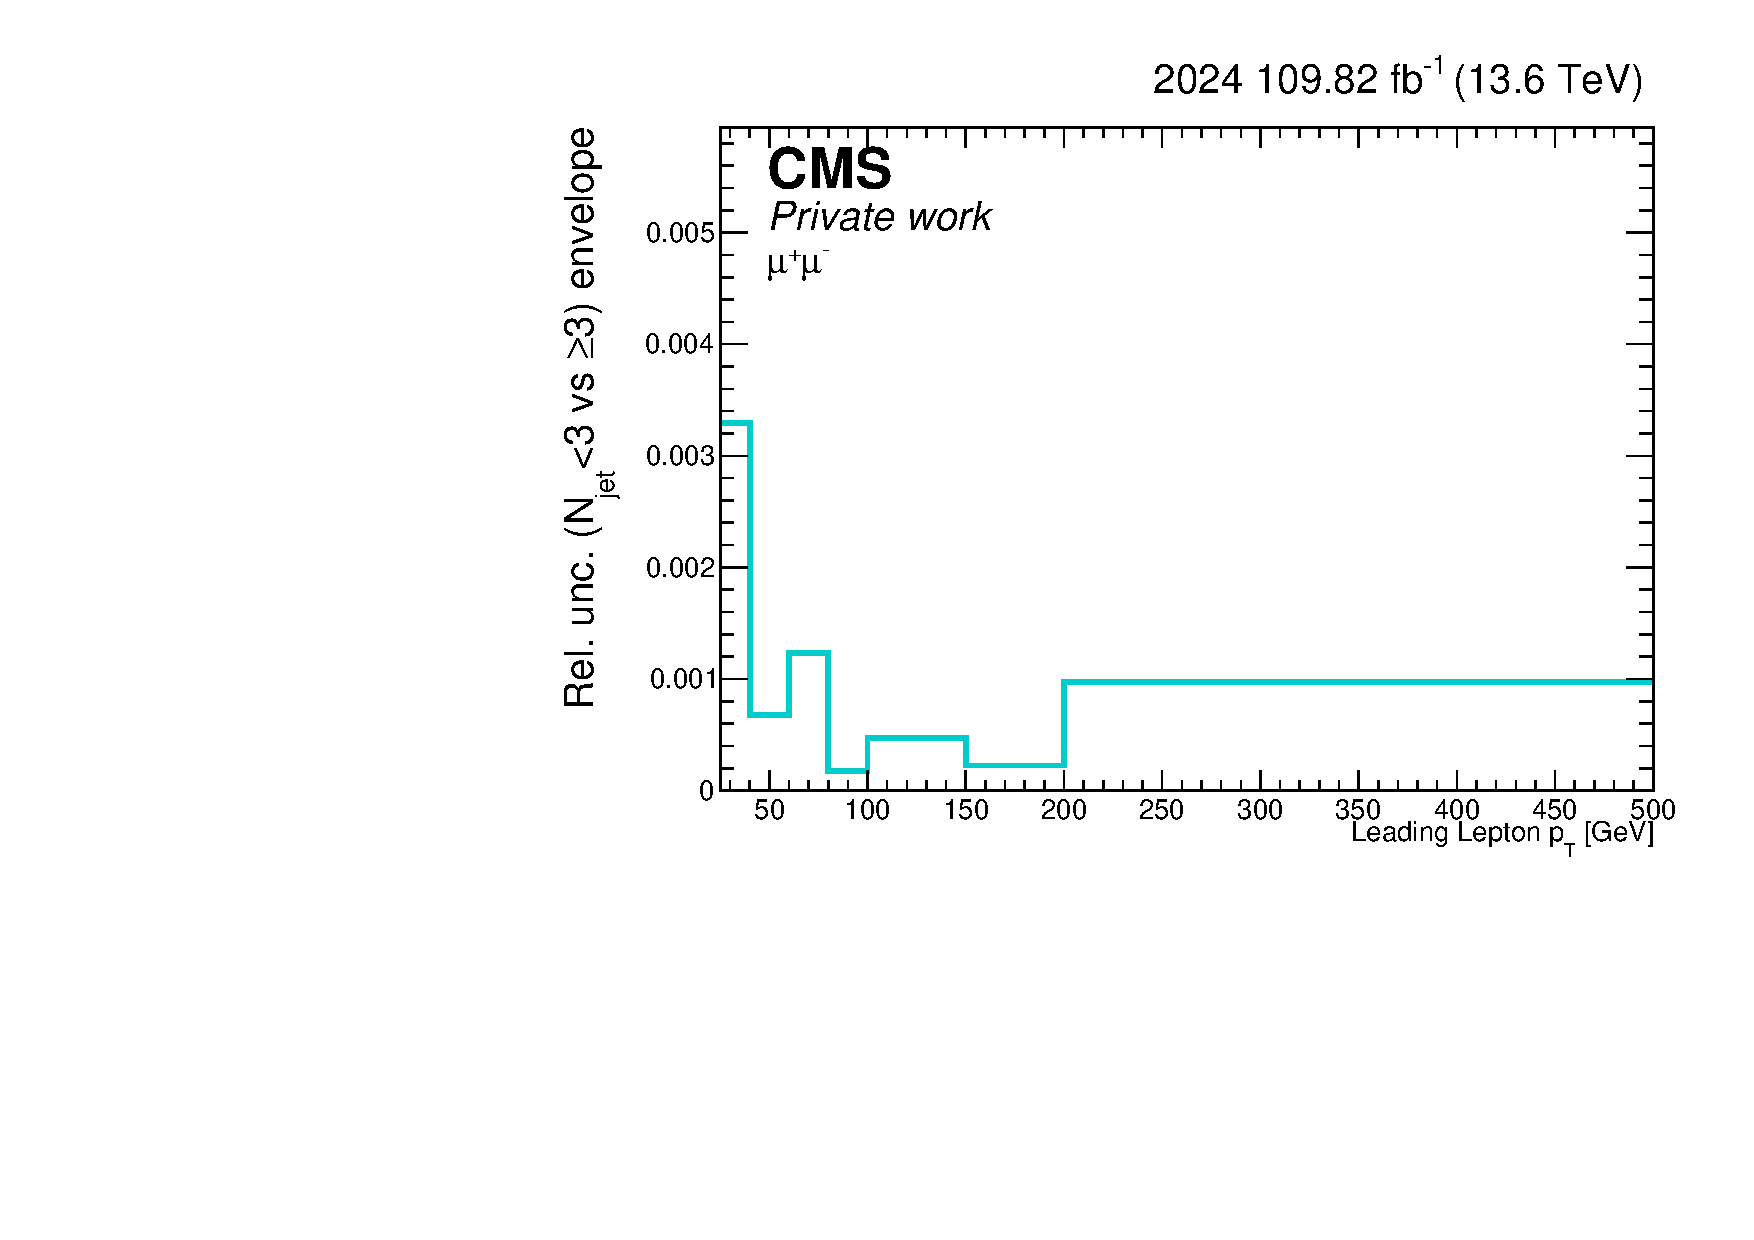
\includegraphics[width=0.48\linewidth]{figures/2024/MuMu/Jet_Topology_Uncertainty/TopoJetUnc_Lep1pt.pdf}
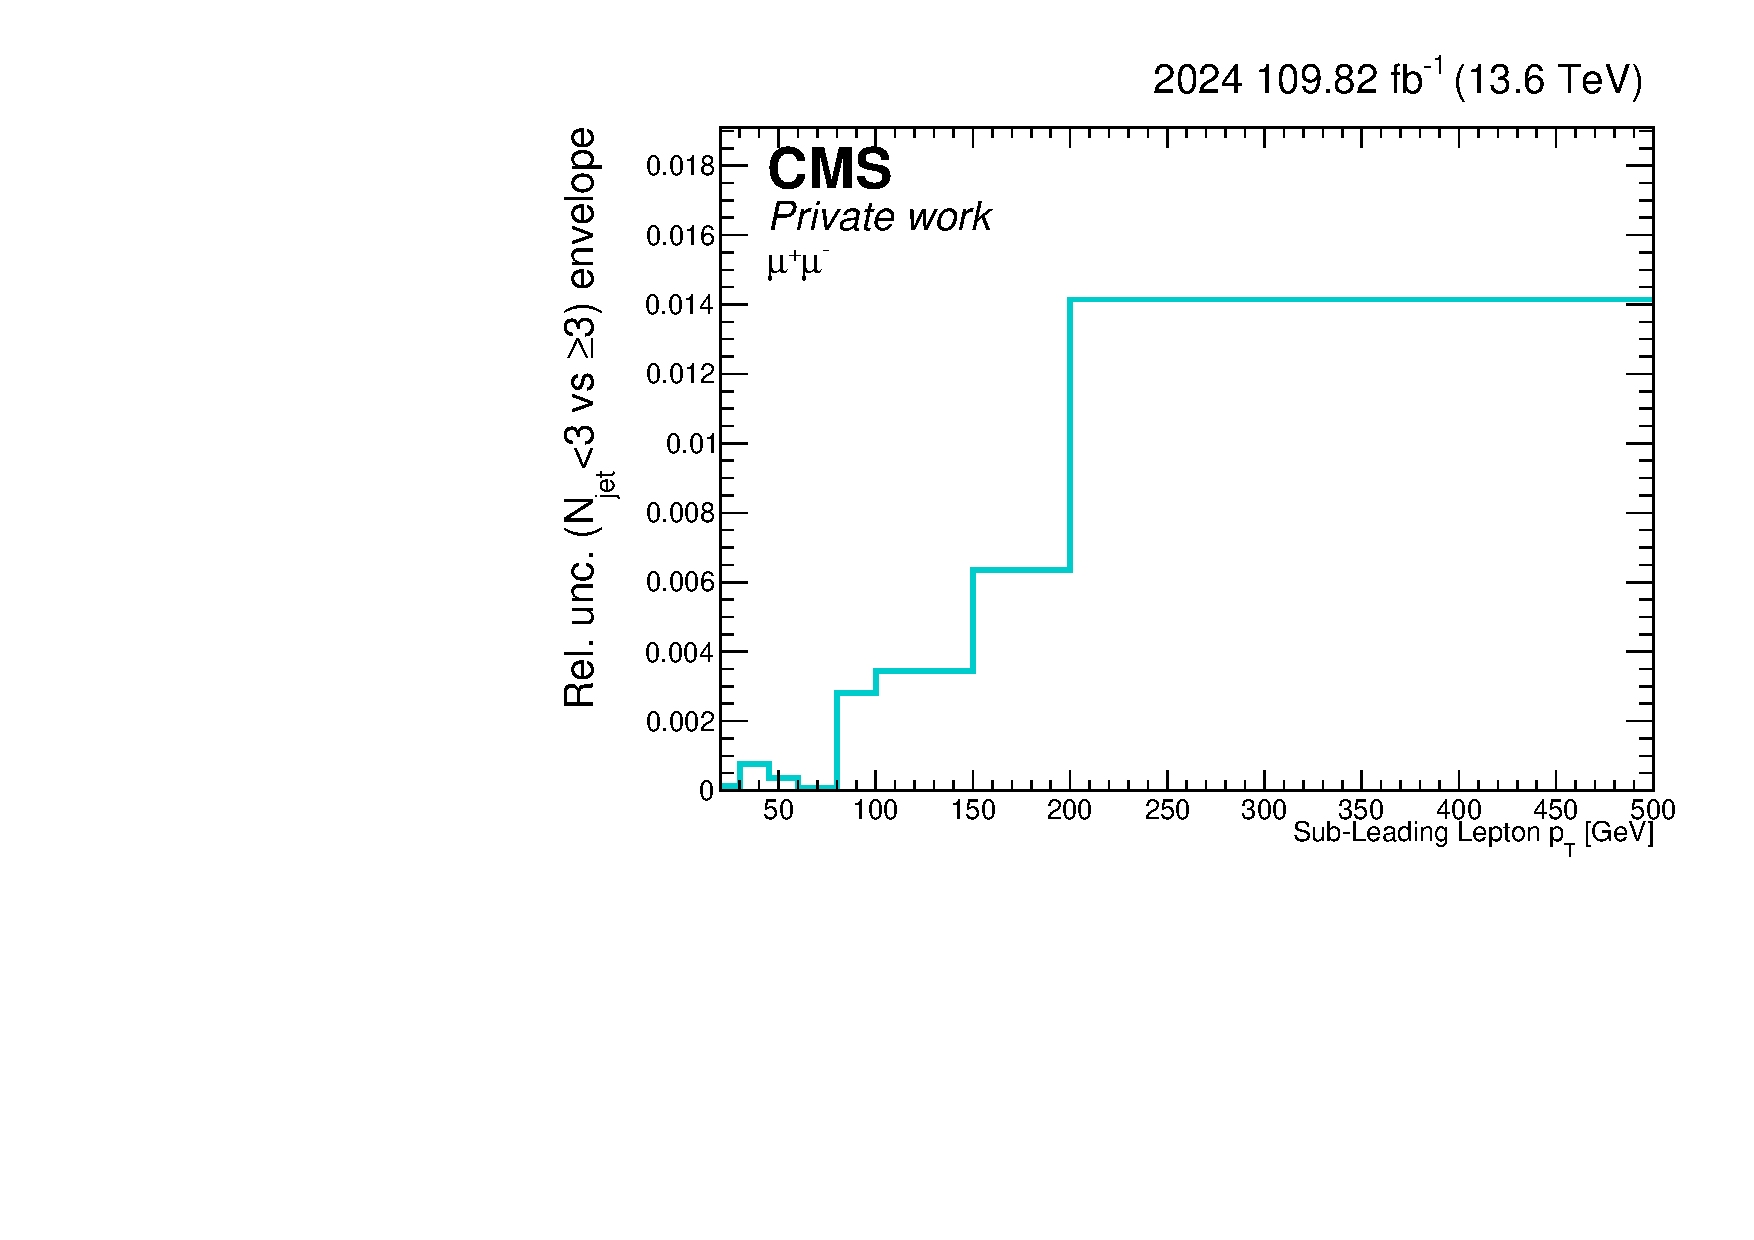
\includegraphics[width=0.48\linewidth]{figures/2024/MuMu/Jet_Topology_Uncertainty/TopoJetUnc_Lep2pt.pdf}
\caption{Jet Topology Uncertainty diagnostics in the $\mu\mu$ channel versus leading and subleading lepton momentum. Curves are reproduced with the production definitions; their exact numerical prescription requires confirmation.}\label{fig:study-MuMu-TopoJetUnc}
\end{figure}
\begin{figure}[htbp]\centering
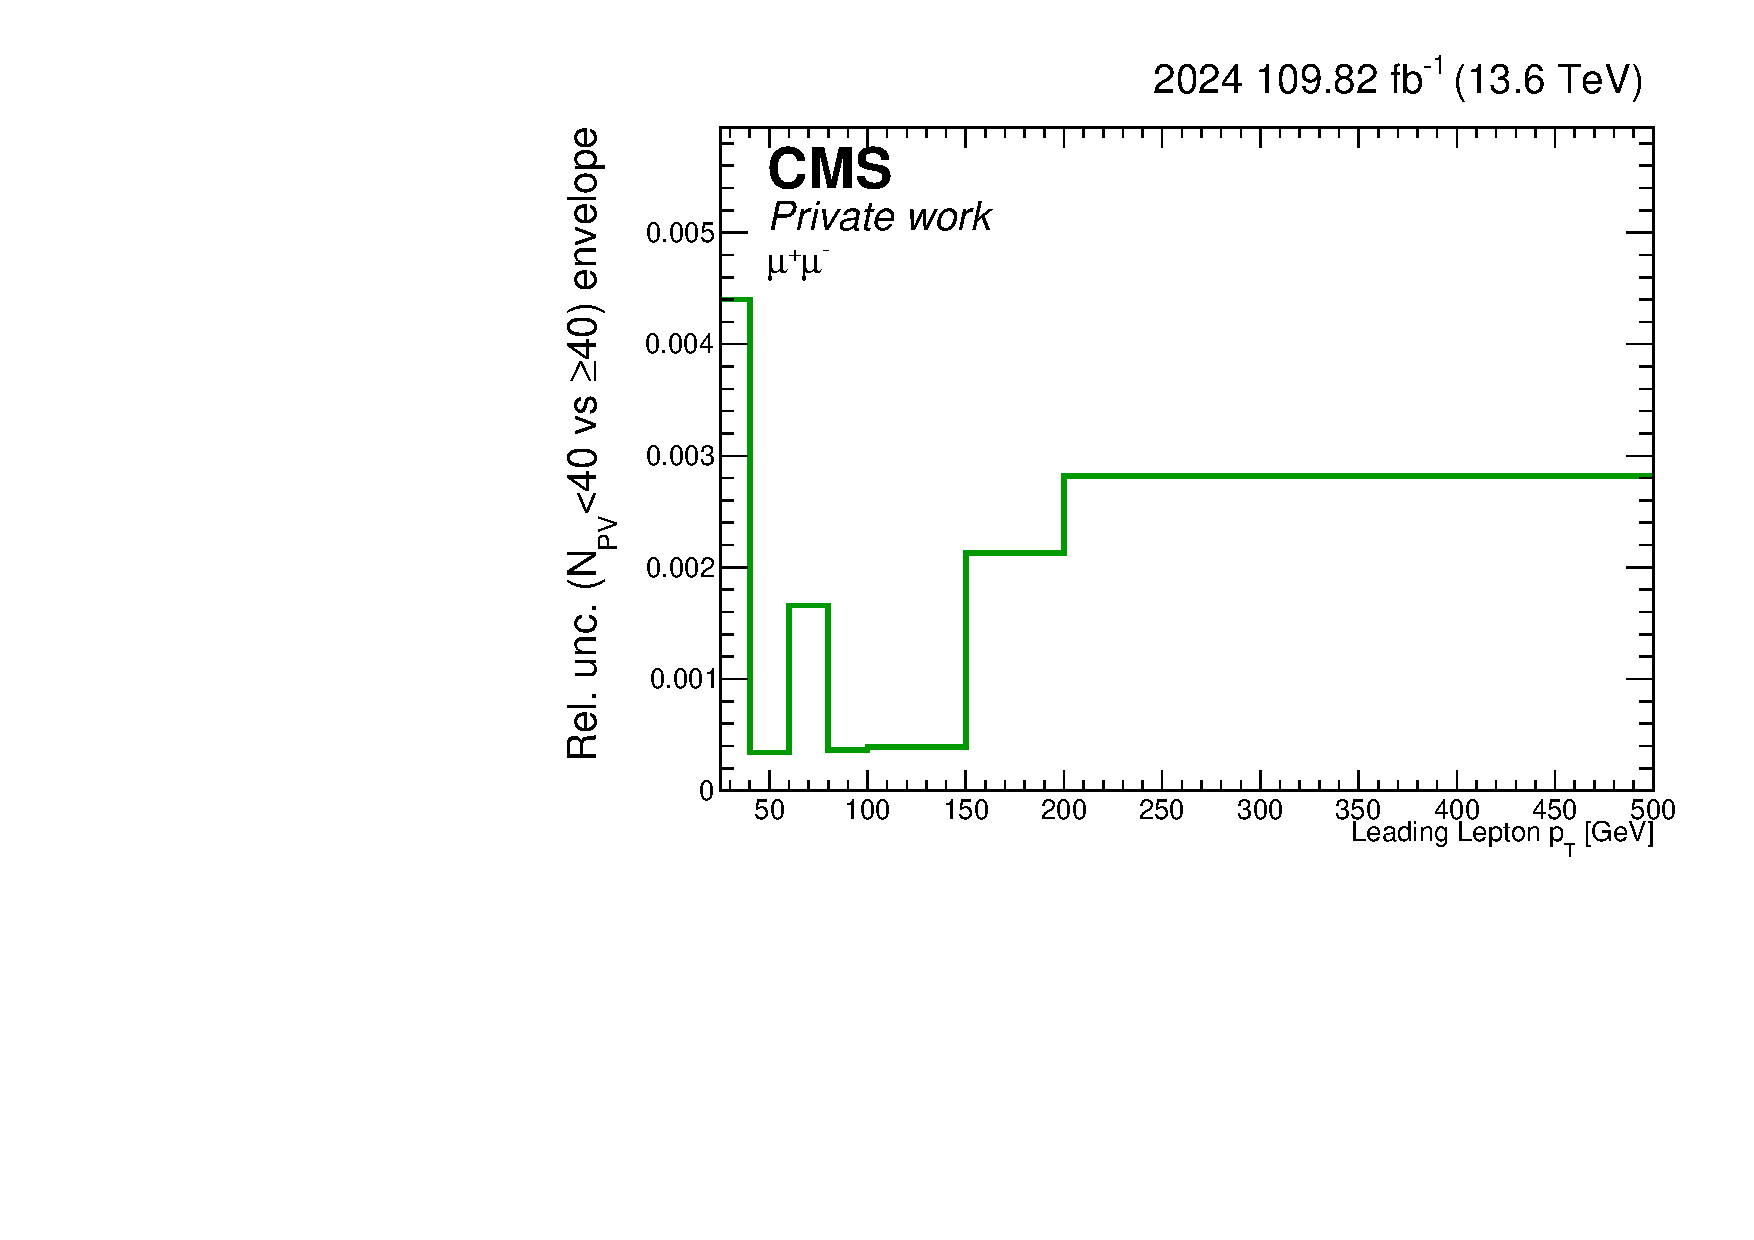
\includegraphics[width=0.48\linewidth]{figures/2024/MuMu/PV_Topology_Uncertainty/TopoPVUnc_Lep1pt.pdf}
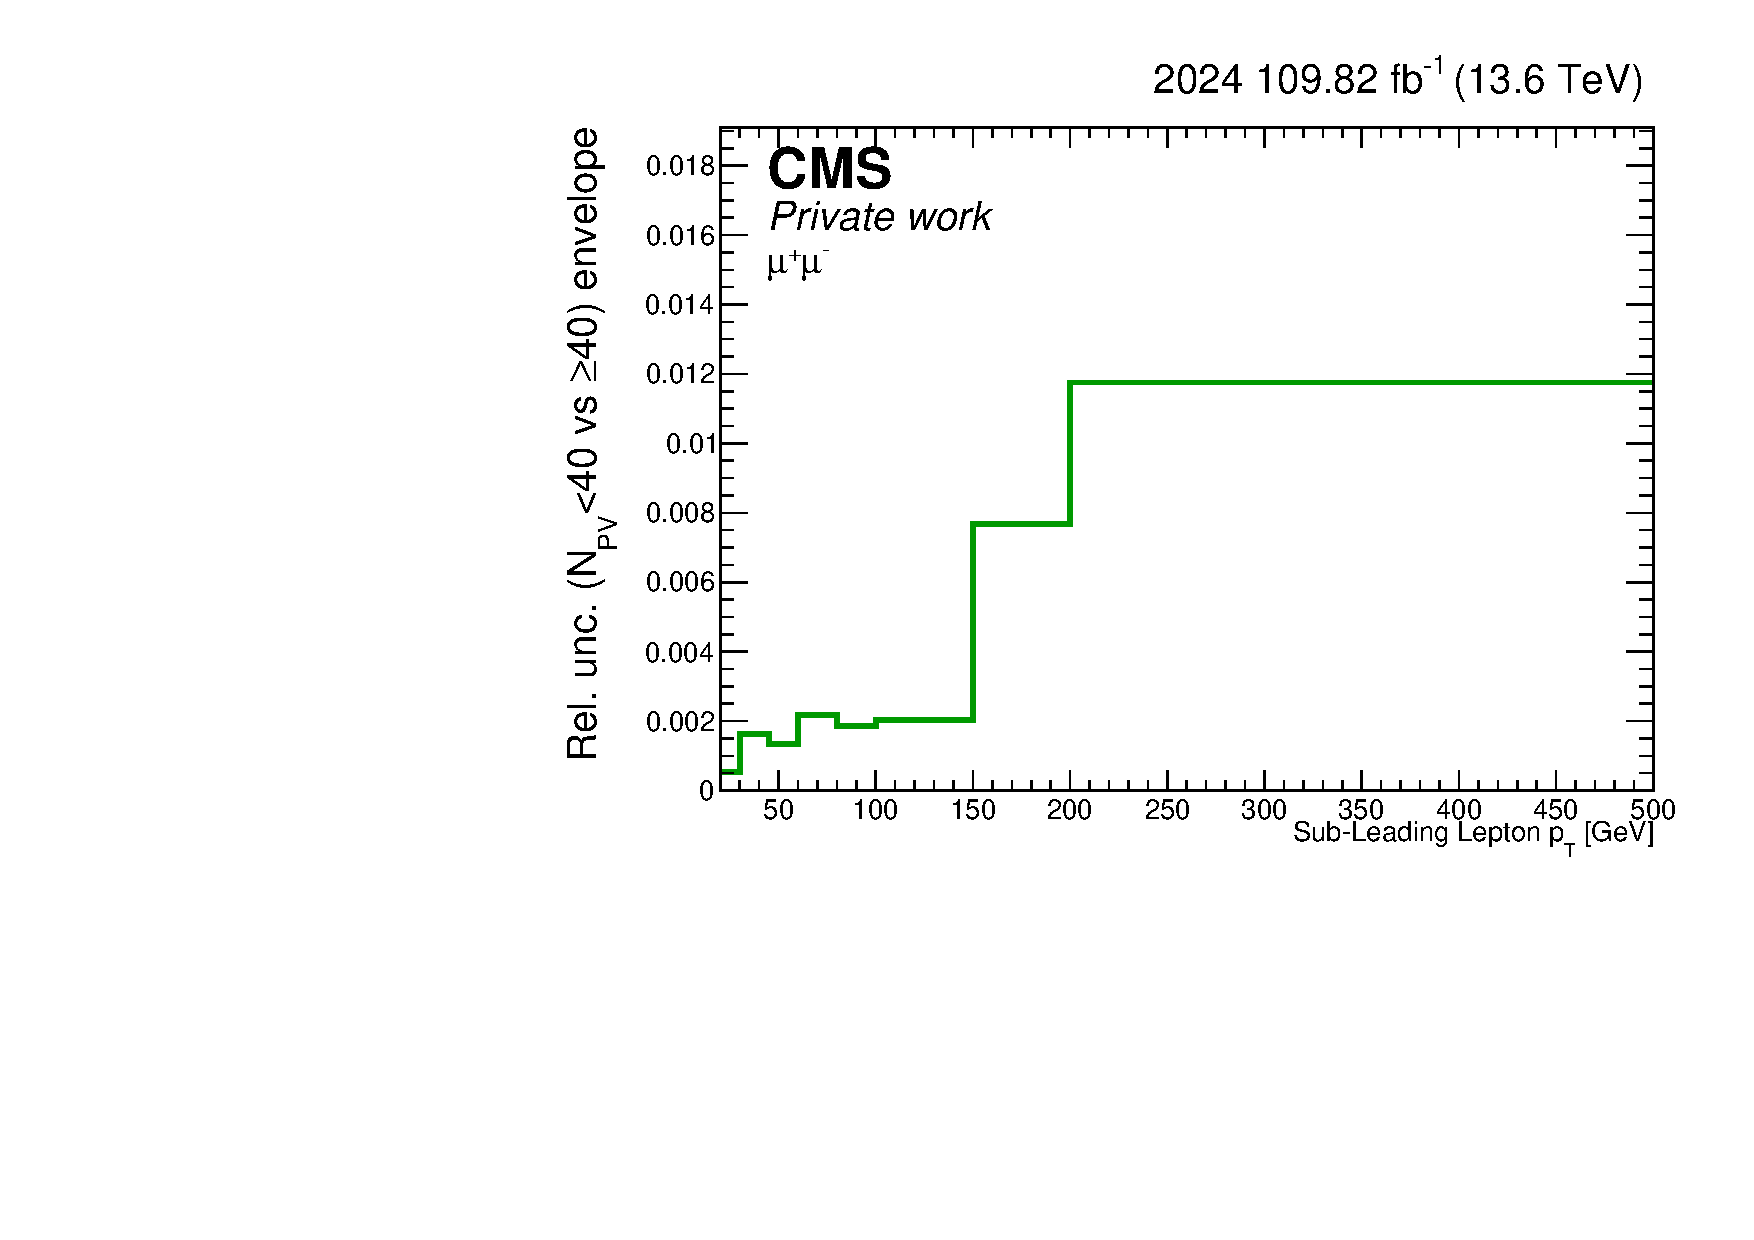
\includegraphics[width=0.48\linewidth]{figures/2024/MuMu/PV_Topology_Uncertainty/TopoPVUnc_Lep2pt.pdf}
\caption{PV Topology Uncertainty diagnostics in the $\mu\mu$ channel versus leading and subleading lepton momentum. Curves are reproduced with the production definitions; their exact numerical prescription requires confirmation.}\label{fig:study-MuMu-TopoPVUnc}
\end{figure}
\begin{figure}[htbp]\centering
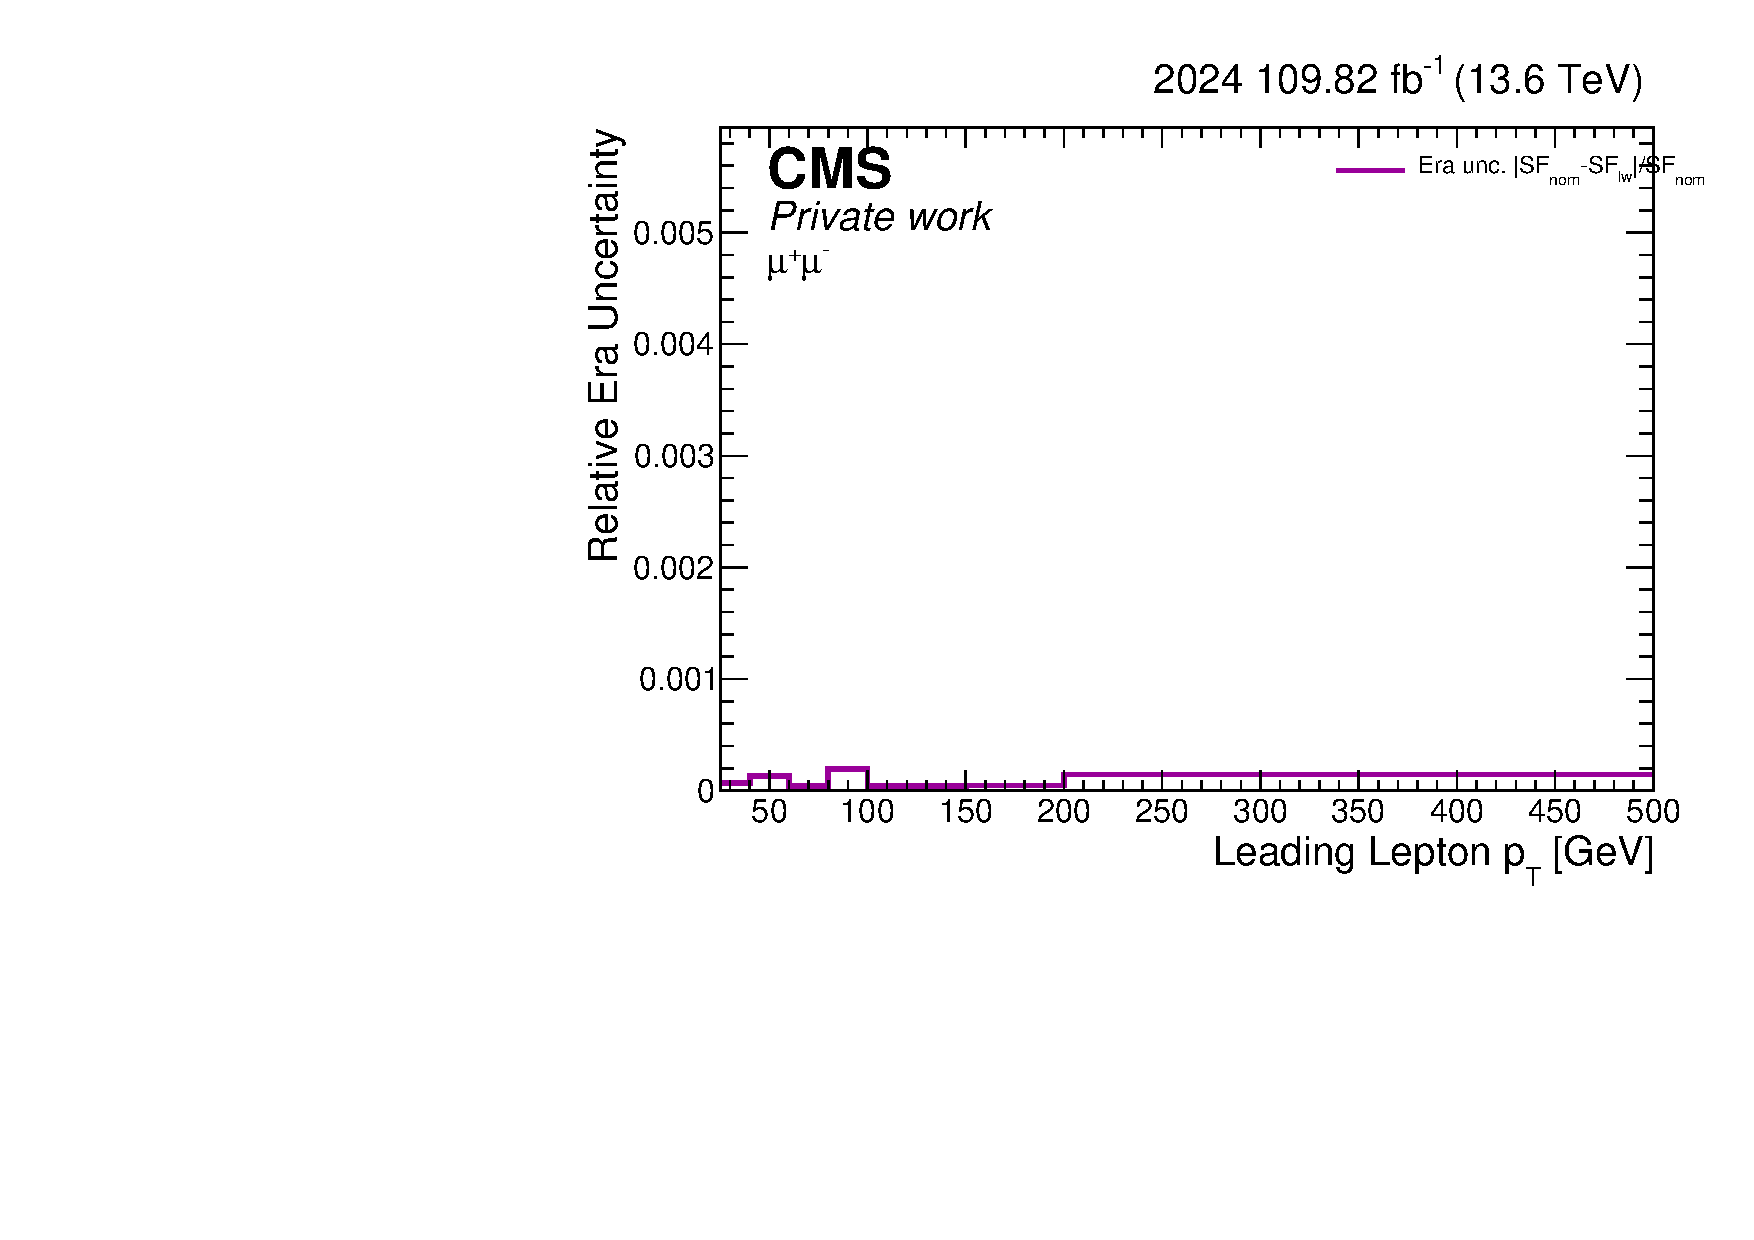
\includegraphics[width=0.48\linewidth]{figures/2024/MuMu/Era_Uncertainty/EraUnc_Lep1pt.pdf}
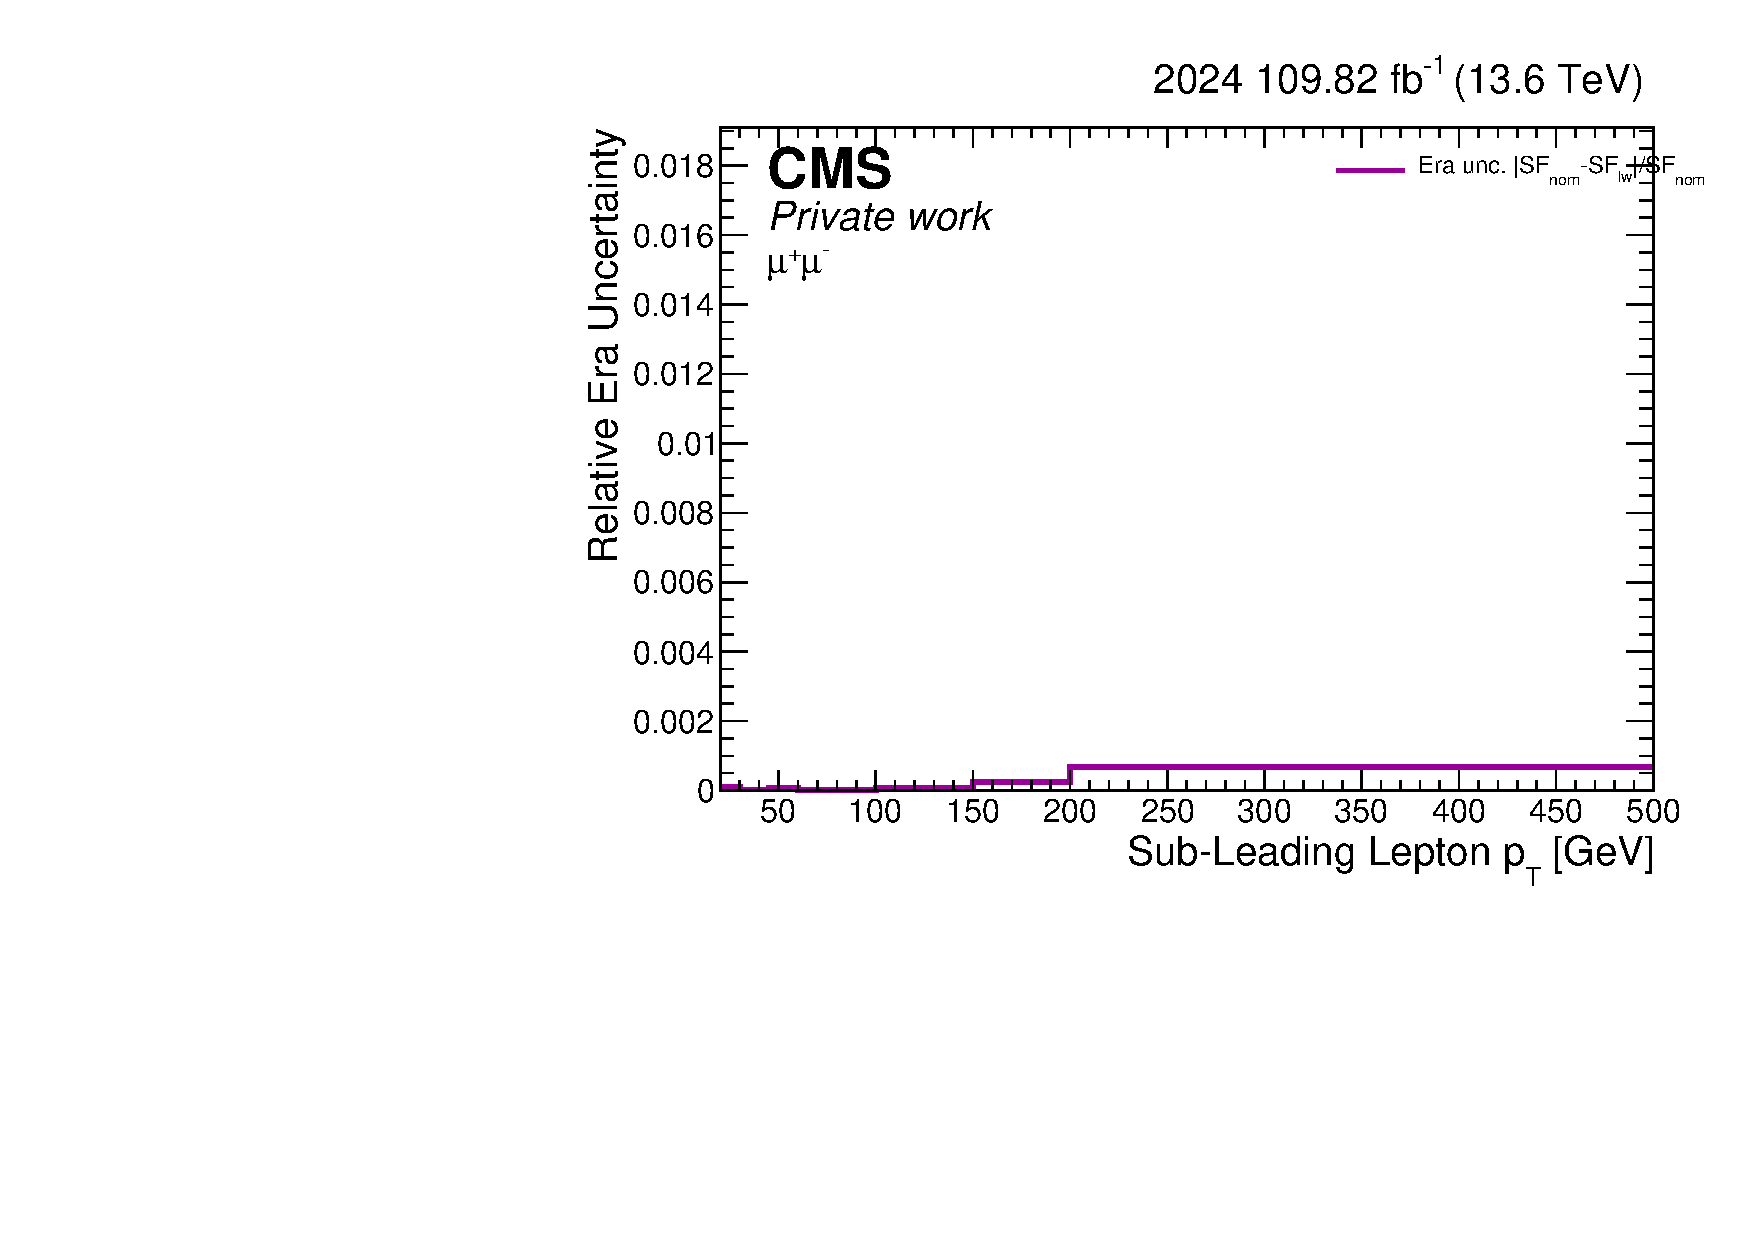
\includegraphics[width=0.48\linewidth]{figures/2024/MuMu/Era_Uncertainty/EraUnc_Lep2pt.pdf}
\caption{Era Uncertainty diagnostics in the $\mu\mu$ channel versus leading and subleading lepton momentum. Curves are reproduced with the production definitions; their exact numerical prescription requires confirmation.}\label{fig:study-MuMu-EraUnc}
\end{figure}
\begin{figure}[htbp]\centering
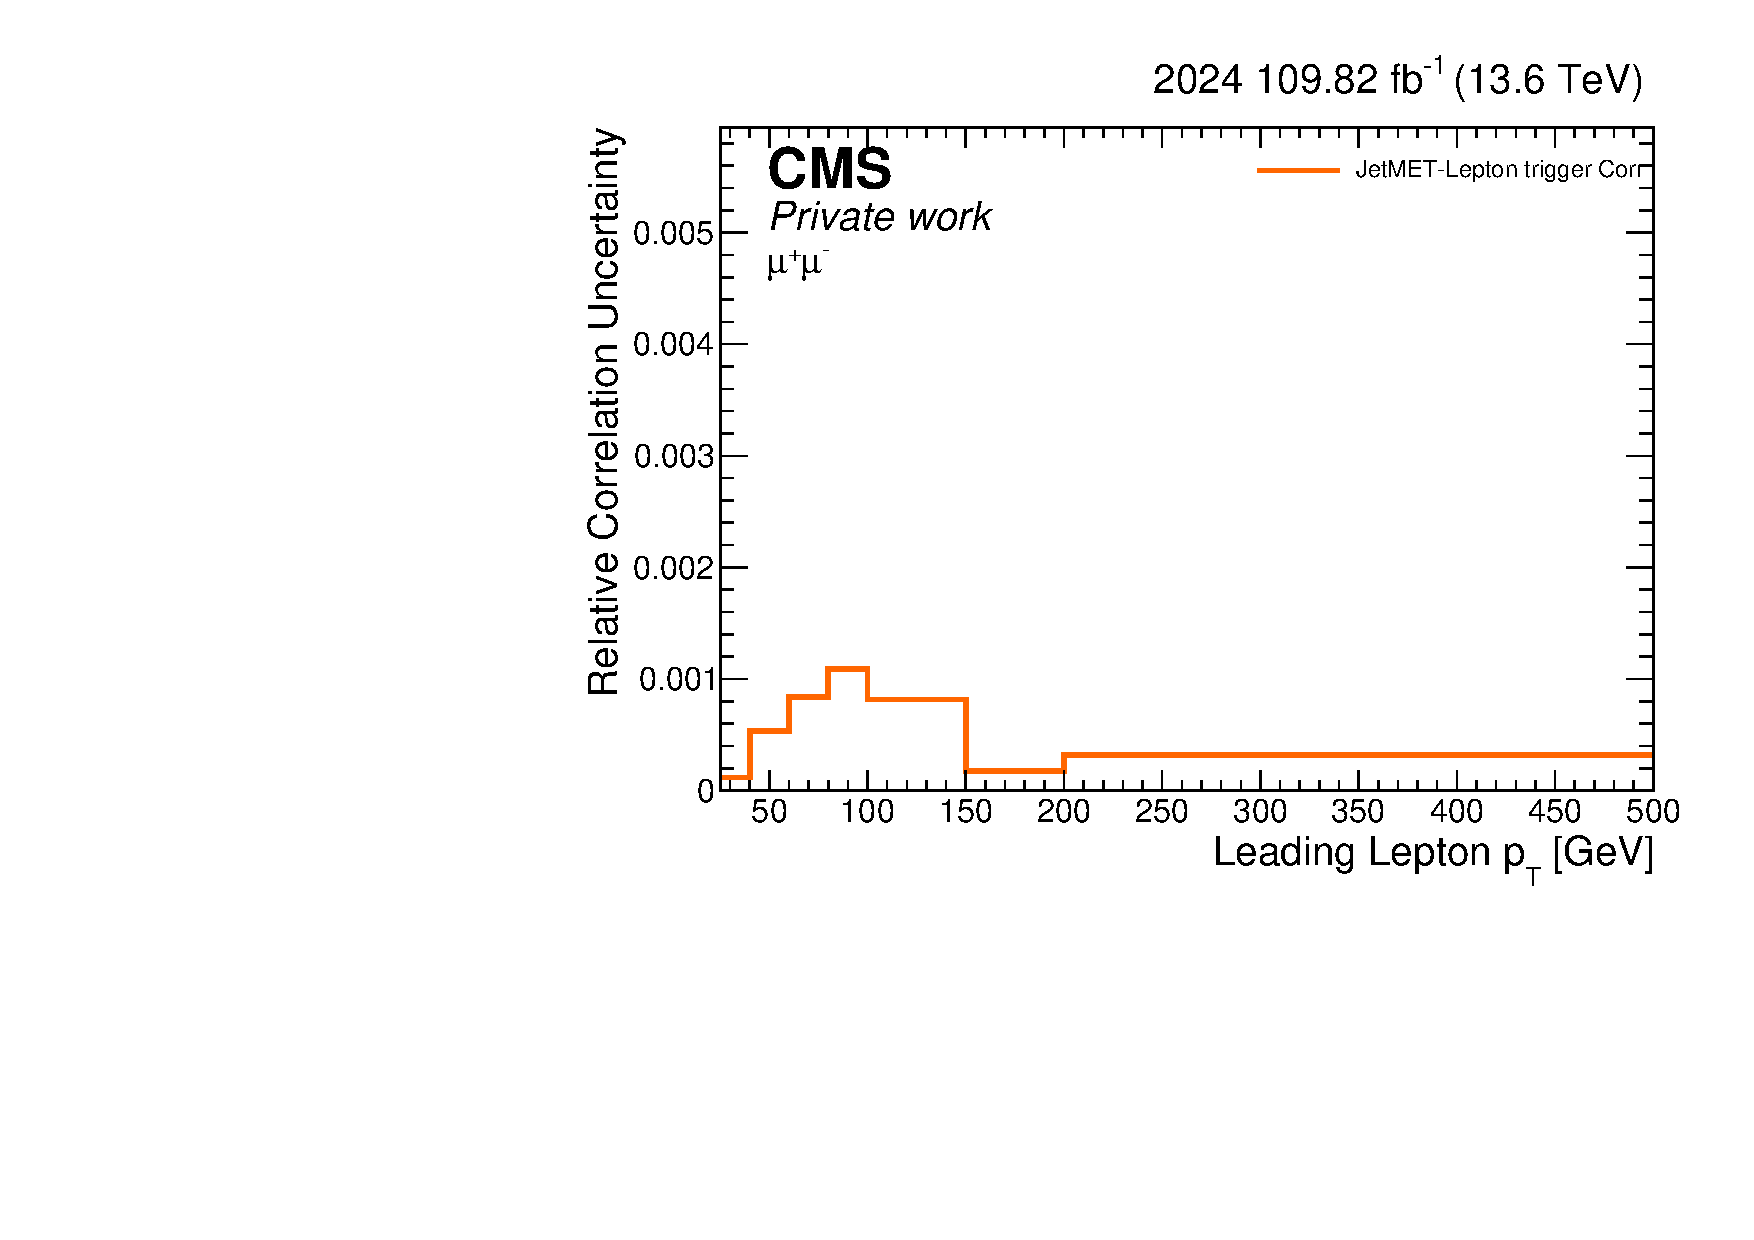
\includegraphics[width=0.48\linewidth]{figures/2024/MuMu/Correlation_Uncertainty/CorrUnc_Lep1pt.pdf}
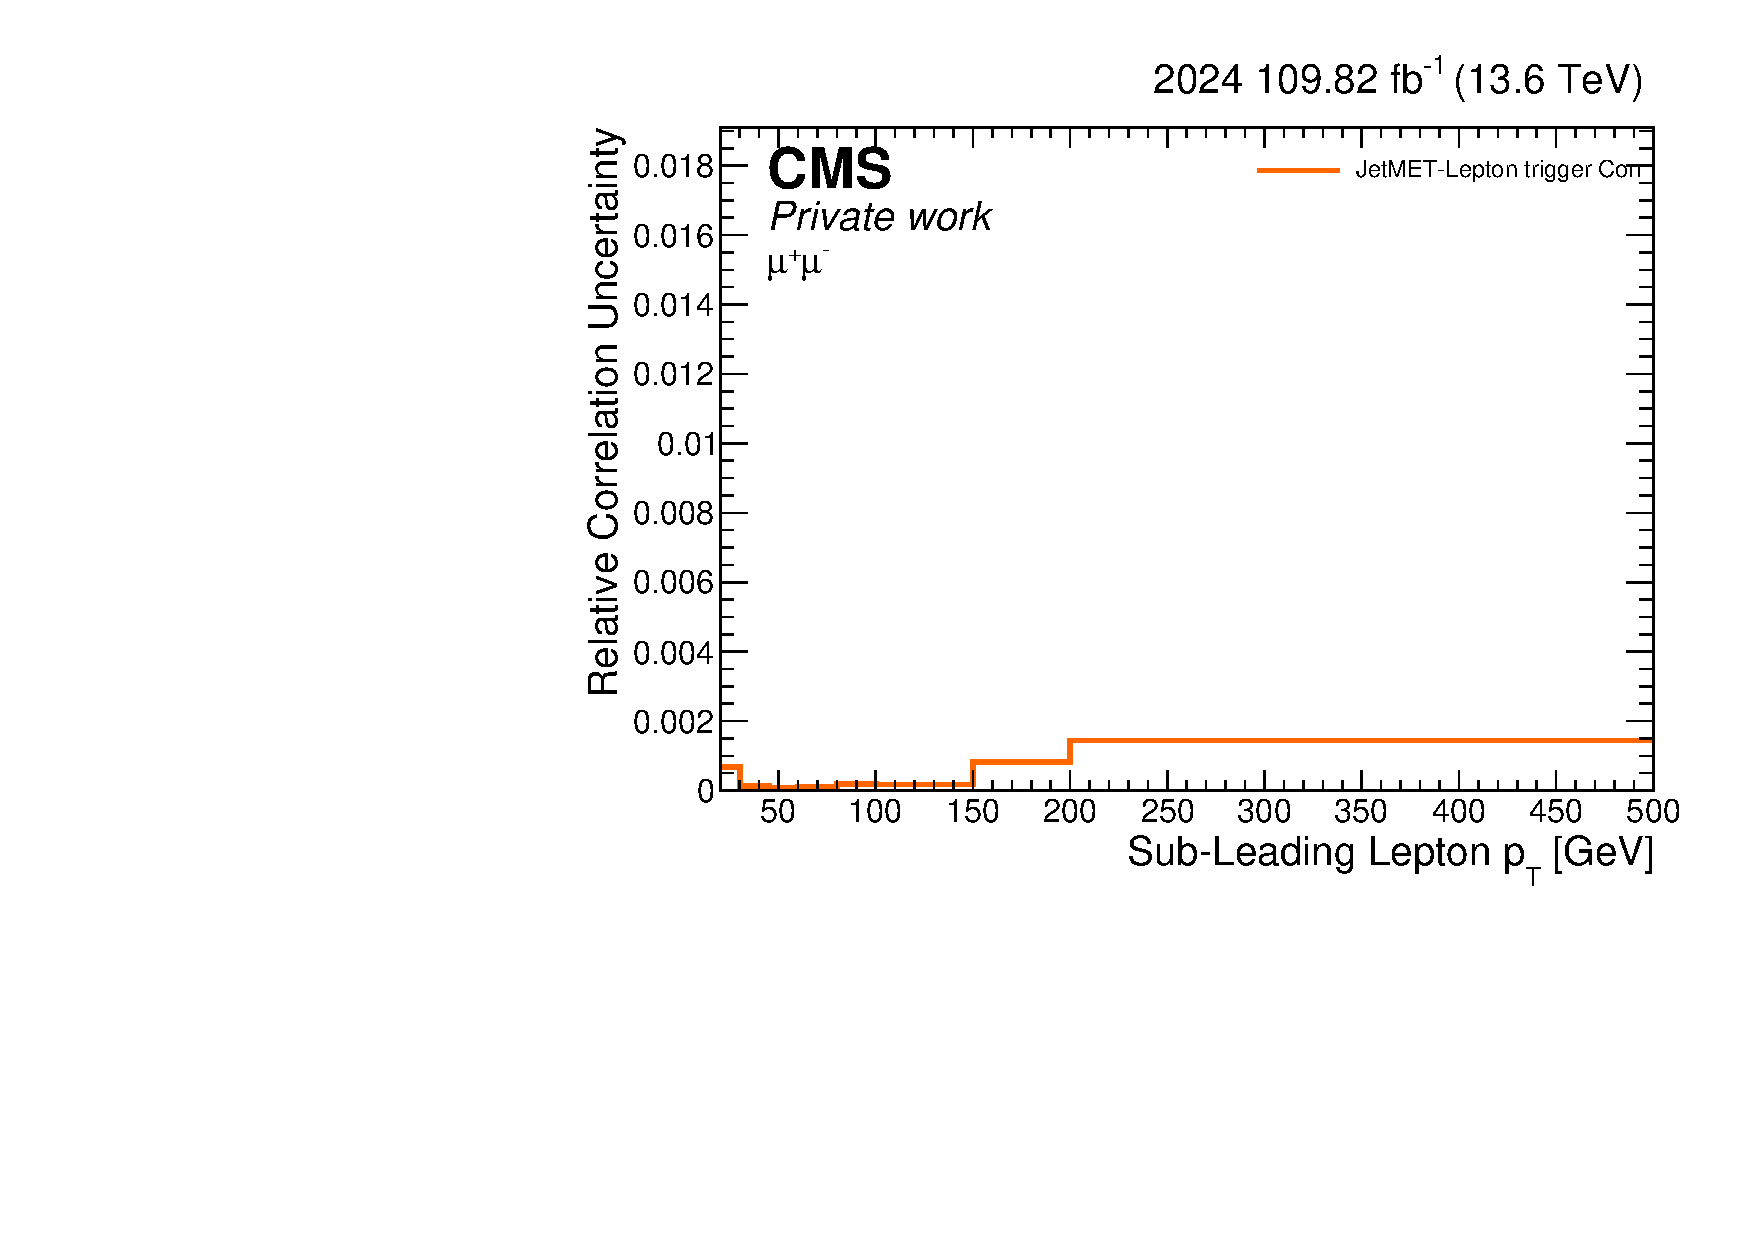
\includegraphics[width=0.48\linewidth]{figures/2024/MuMu/Correlation_Uncertainty/CorrUnc_Lep2pt.pdf}
\caption{Correlation Uncertainty diagnostics in the $\mu\mu$ channel versus leading and subleading lepton momentum. Curves are reproduced with the production definitions; their exact numerical prescription requires confirmation.}\label{fig:study-MuMu-CorrUnc}
\end{figure}

\clearpage\section{Selected 2024 supporting distributions}\label{app:2024-support}
The following distributions document the efficiency inputs, statistical precision, and uncertainty composition for the 2024 measurement. Only inclusive distributions directly related to the correction or its principal checks are selected. The jet- and vertex-split variants and the full set of individual-jet and angular distributions are not reproduced. These plots use the measurement sample and are not independent closure tests.
\subsection{$ee$ channel}
\begin{figure}[htbp]\centering
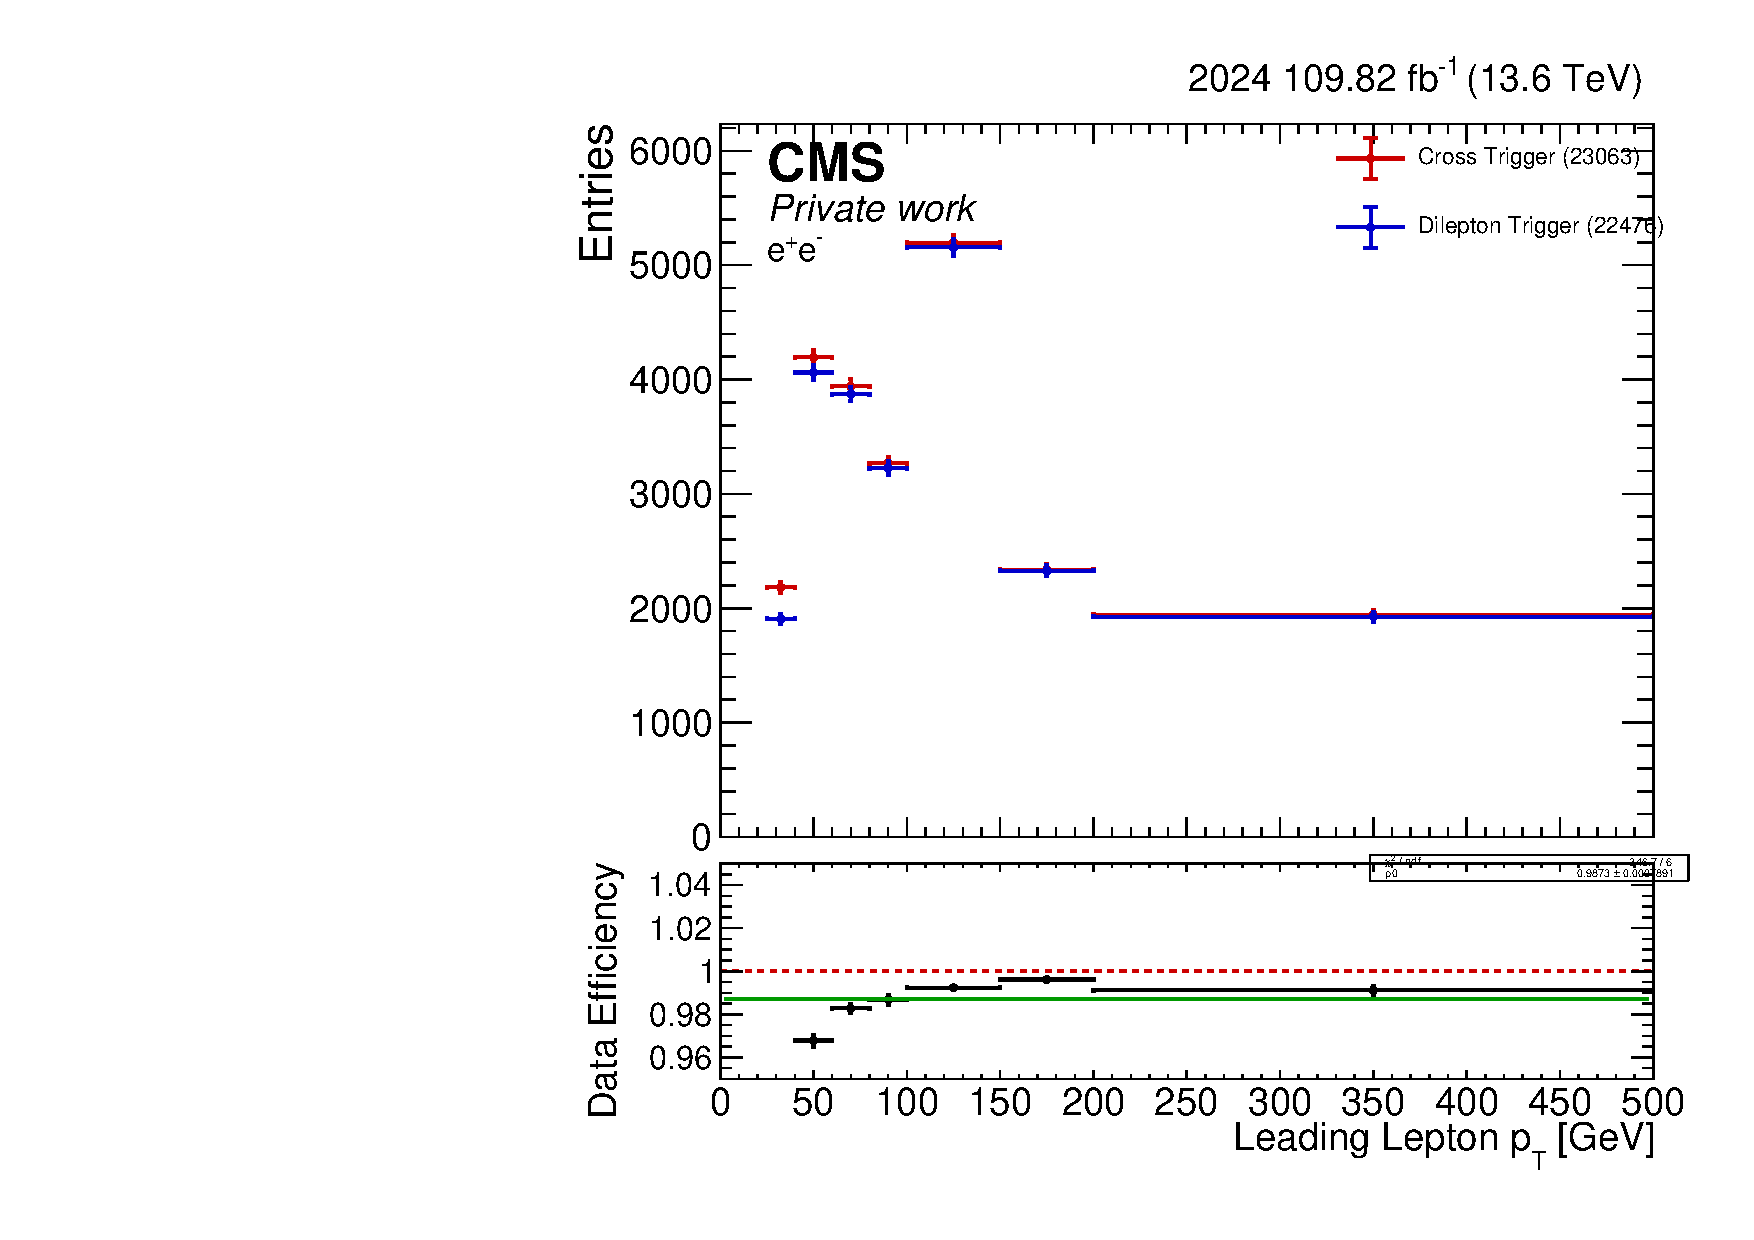
\includegraphics[width=0.48\linewidth]{figures/2024/ElEl/TrigEffData/TrigEff_Lep1pt.pdf}
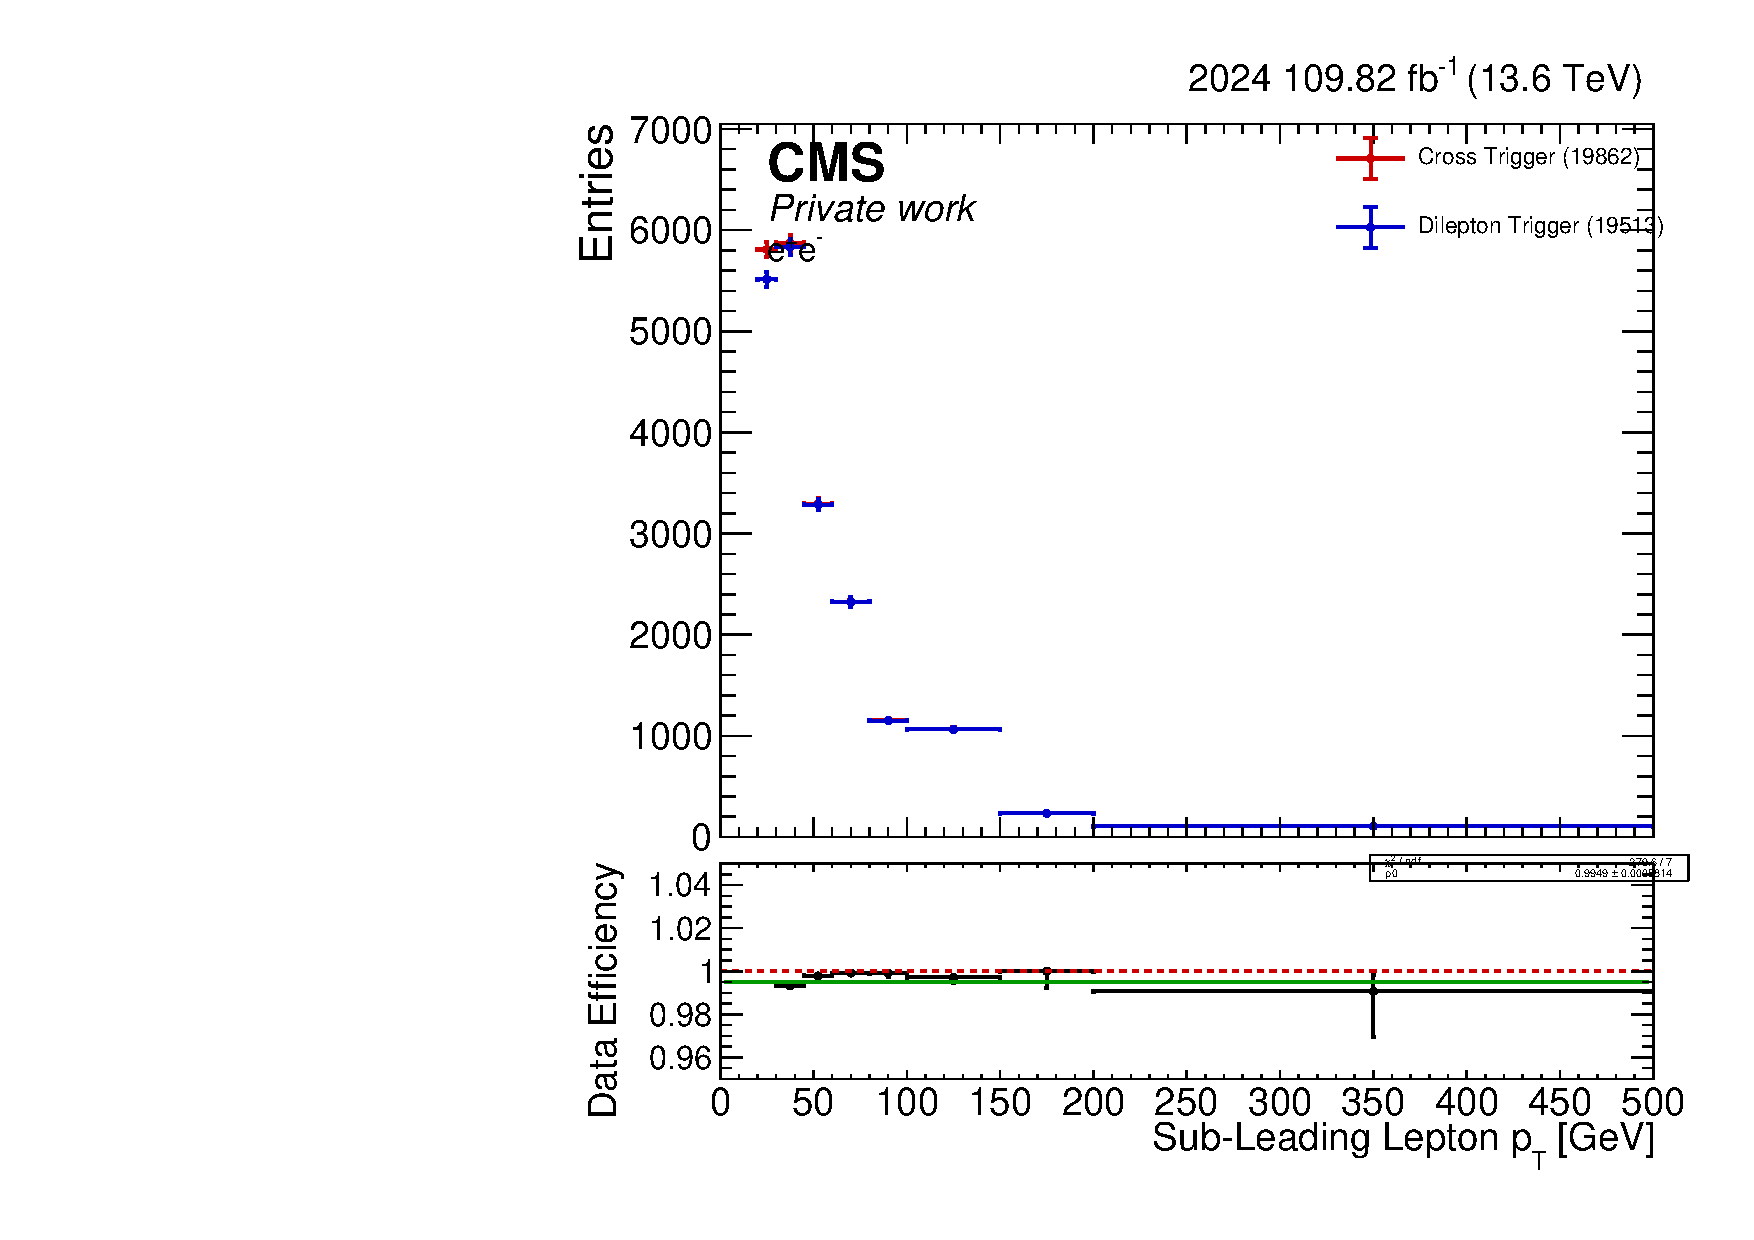
\includegraphics[width=0.48\linewidth]{figures/2024/ElEl/TrigEffData/TrigEff_Lep2pt.pdf}
\caption{Data trigger numerator and reference-sample distributions (upper panels), with their efficiency ratios (lower panels) in the $ee$ channel. Left and right: leading and subleading lepton $p_{\mathrm{T}}$.}\label{fig:extra-ElEl-TrigEffData-Lep1pt}\end{figure}
\begin{figure}[p]\centering
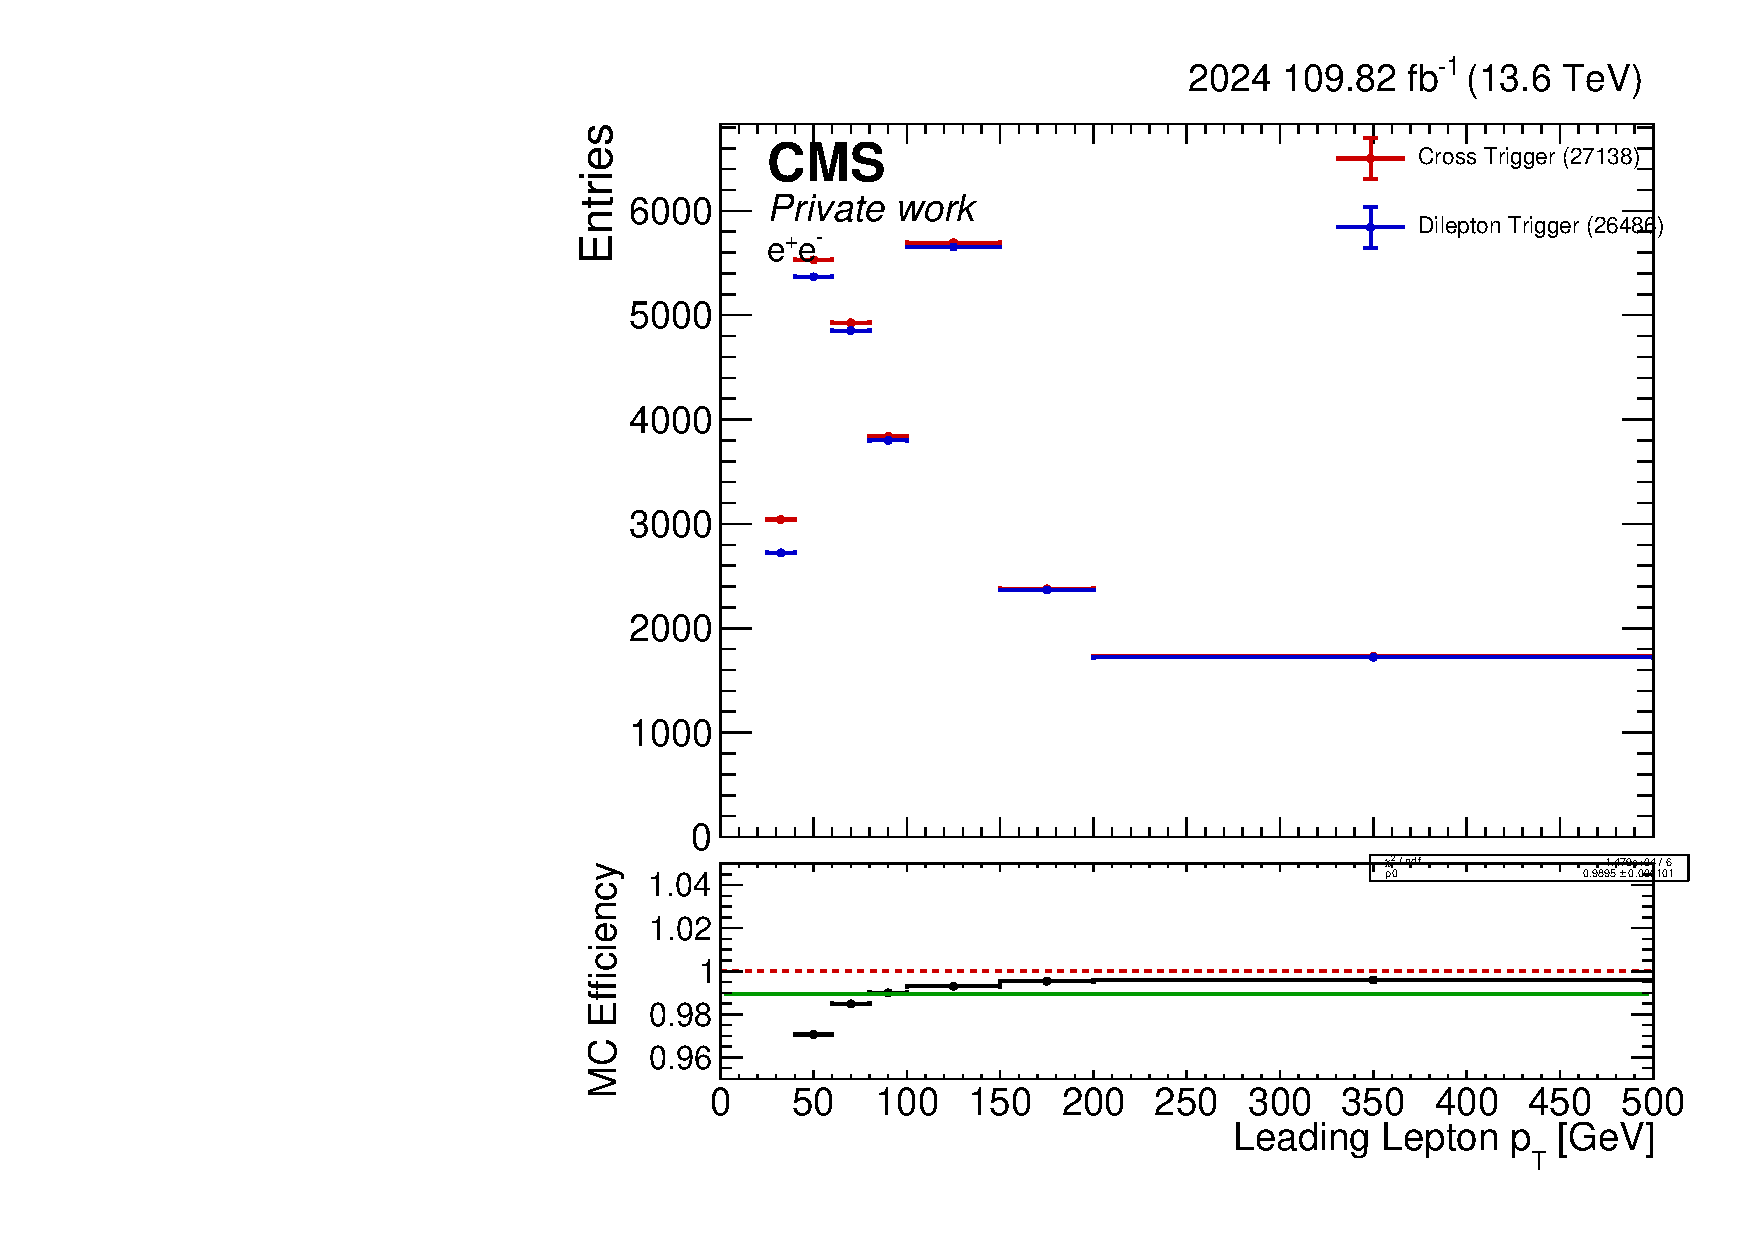
\includegraphics[width=0.48\linewidth]{figures/2024/ElEl/TrigEffMC/TrigEff_Lep1pt.pdf}
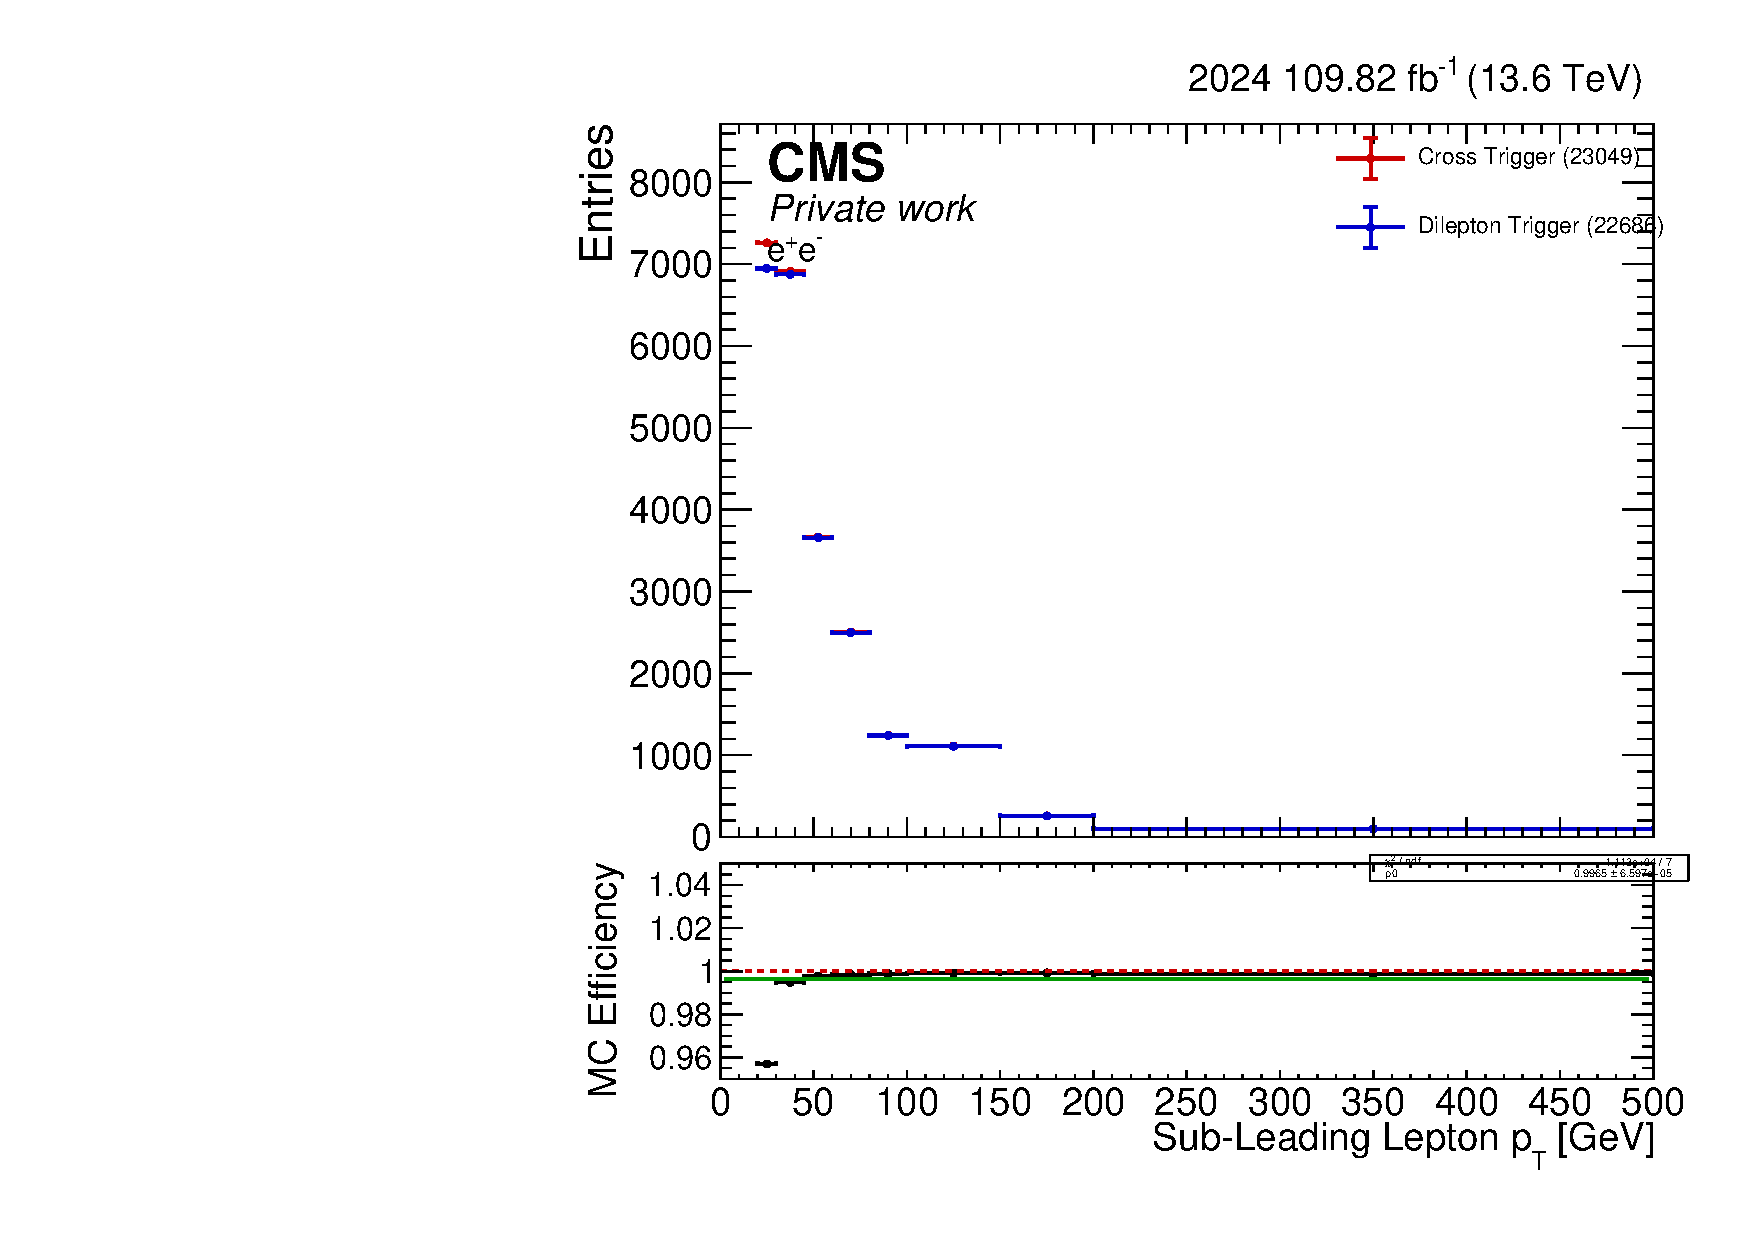
\includegraphics[width=0.48\linewidth]{figures/2024/ElEl/TrigEffMC/TrigEff_Lep2pt.pdf}
\caption{Simulated trigger numerator and reference-sample distributions (upper panels), with their efficiency ratios (lower panels) in the $ee$ channel. Left and right: leading and subleading lepton $p_{\mathrm{T}}$.}\label{fig:extra-ElEl-TrigEffMC-Lep1pt}\end{figure}
\begin{figure}[p]\centering
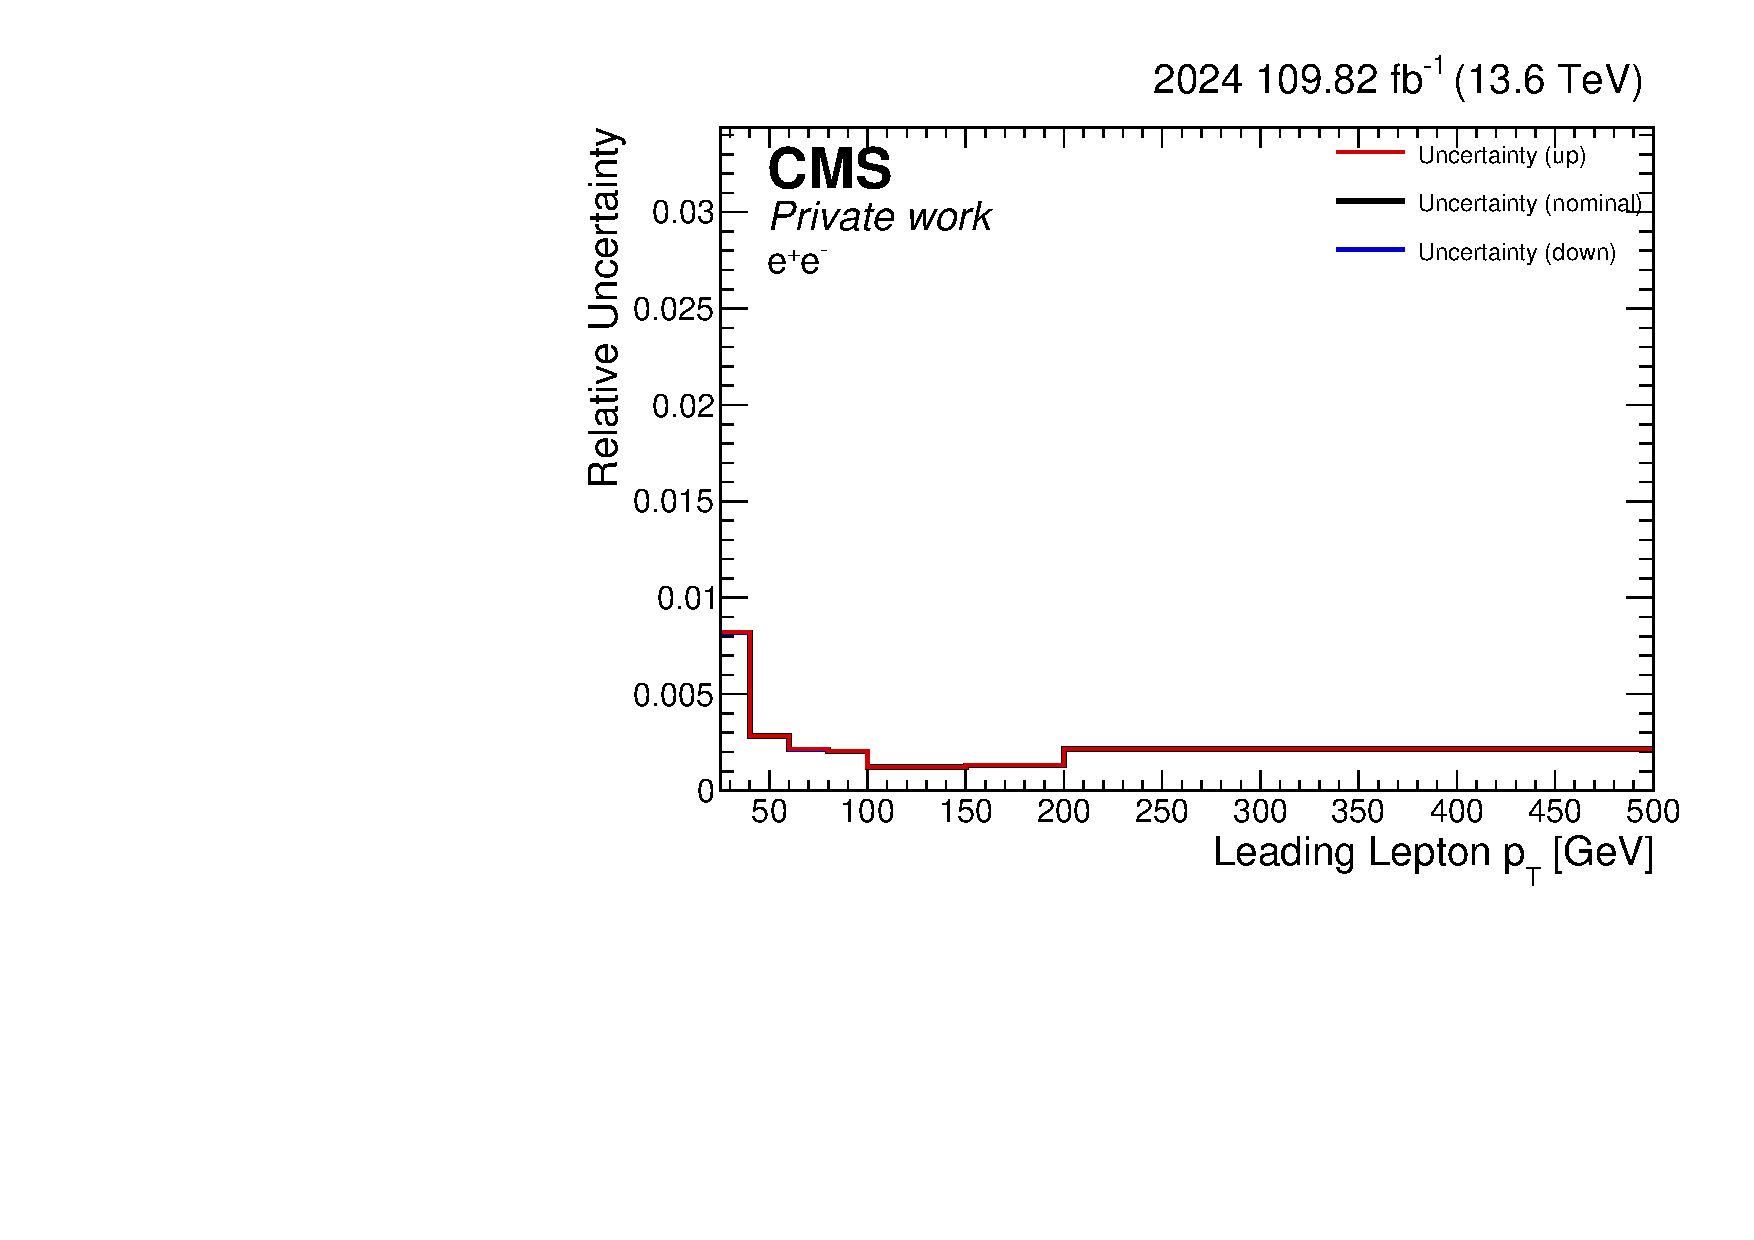
\includegraphics[width=0.48\linewidth]{figures/2024/ElEl/Statistical_Uncertainty/UncRatio_Lep1pt.pdf}
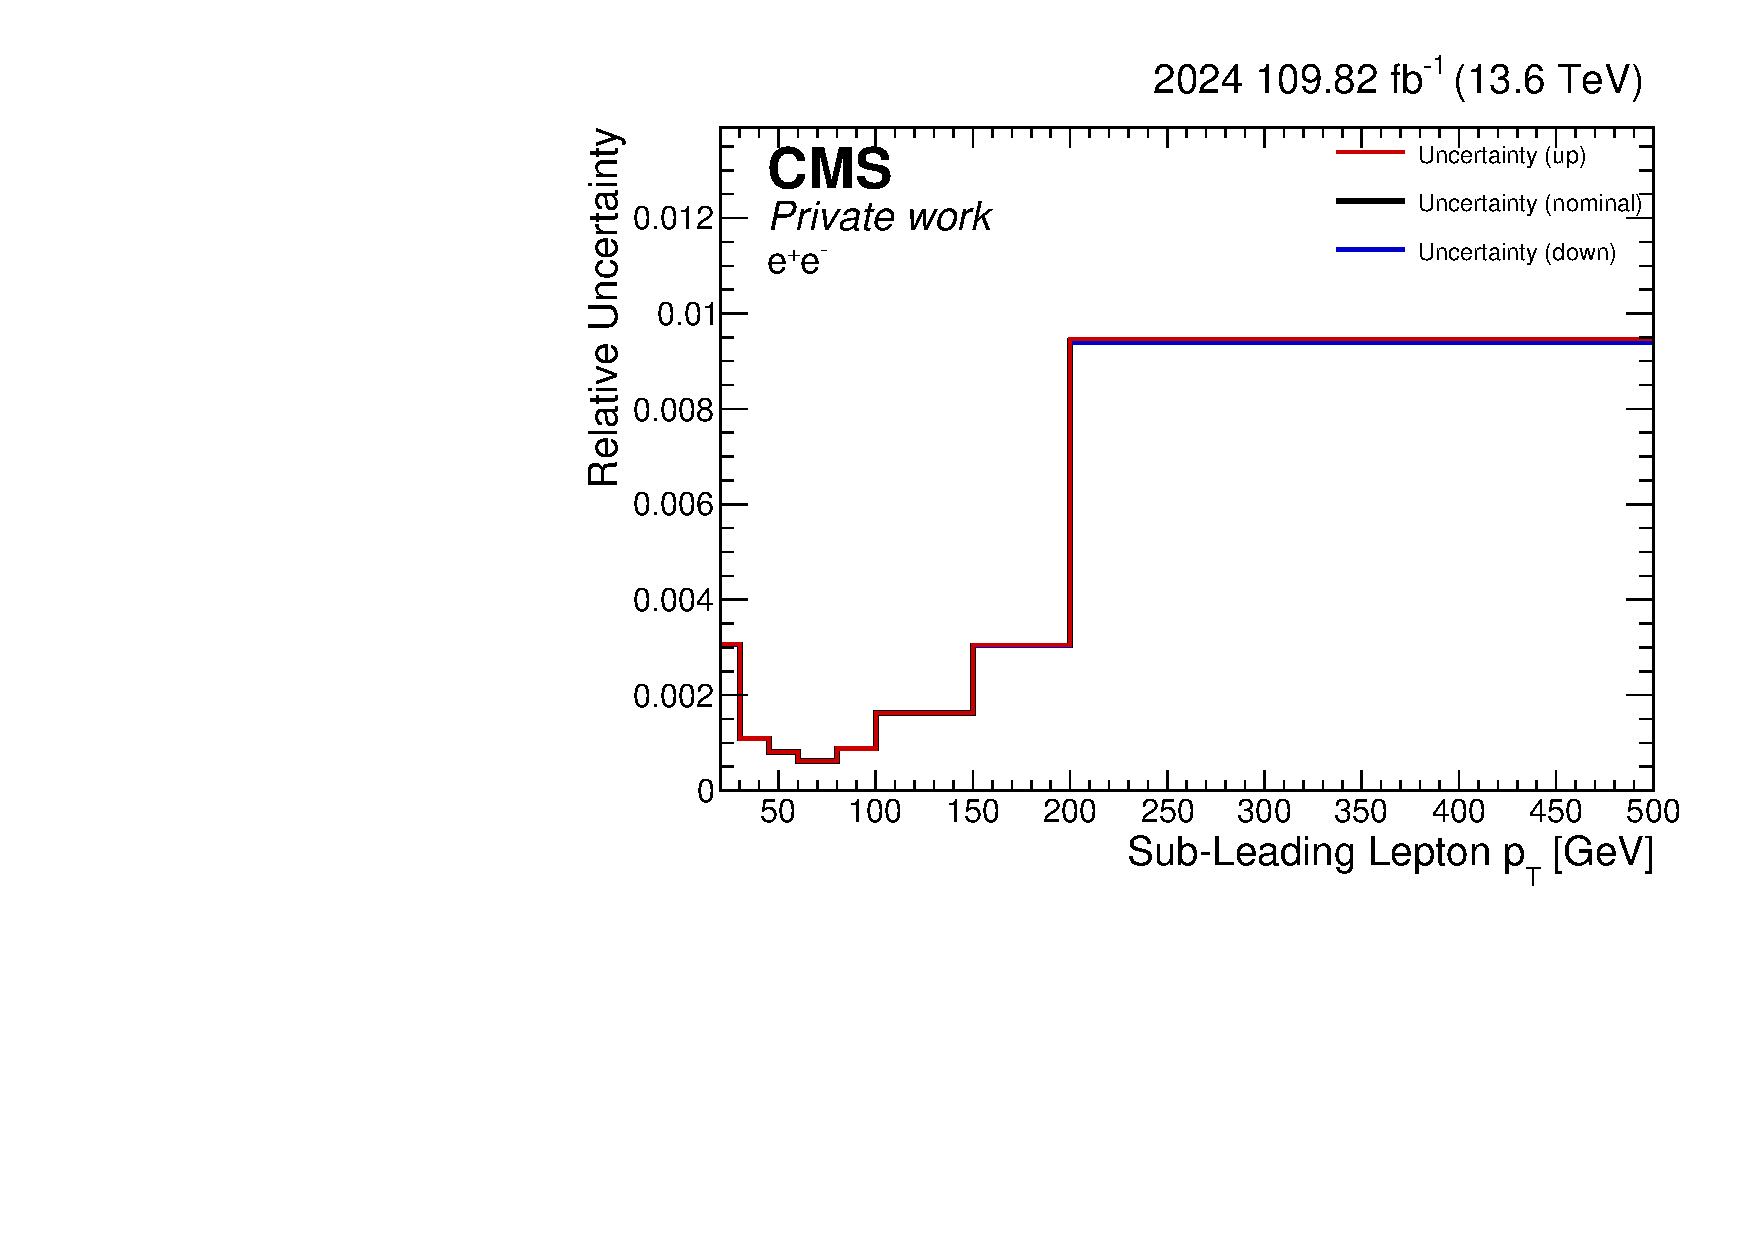
\includegraphics[width=0.48\linewidth]{figures/2024/ElEl/Statistical_Uncertainty/UncRatio_Lep2pt.pdf}
\caption{Relative statistical uncertainty diagnostics, retaining the nominal, upward, and downward curves of the supplied production in the $ee$ channel. Left and right: leading and subleading lepton $p_{\mathrm{T}}$.}\label{fig:extra-ElEl-Statistical-Uncertainty-Lep1pt}\end{figure}
\begin{figure}[p]\centering
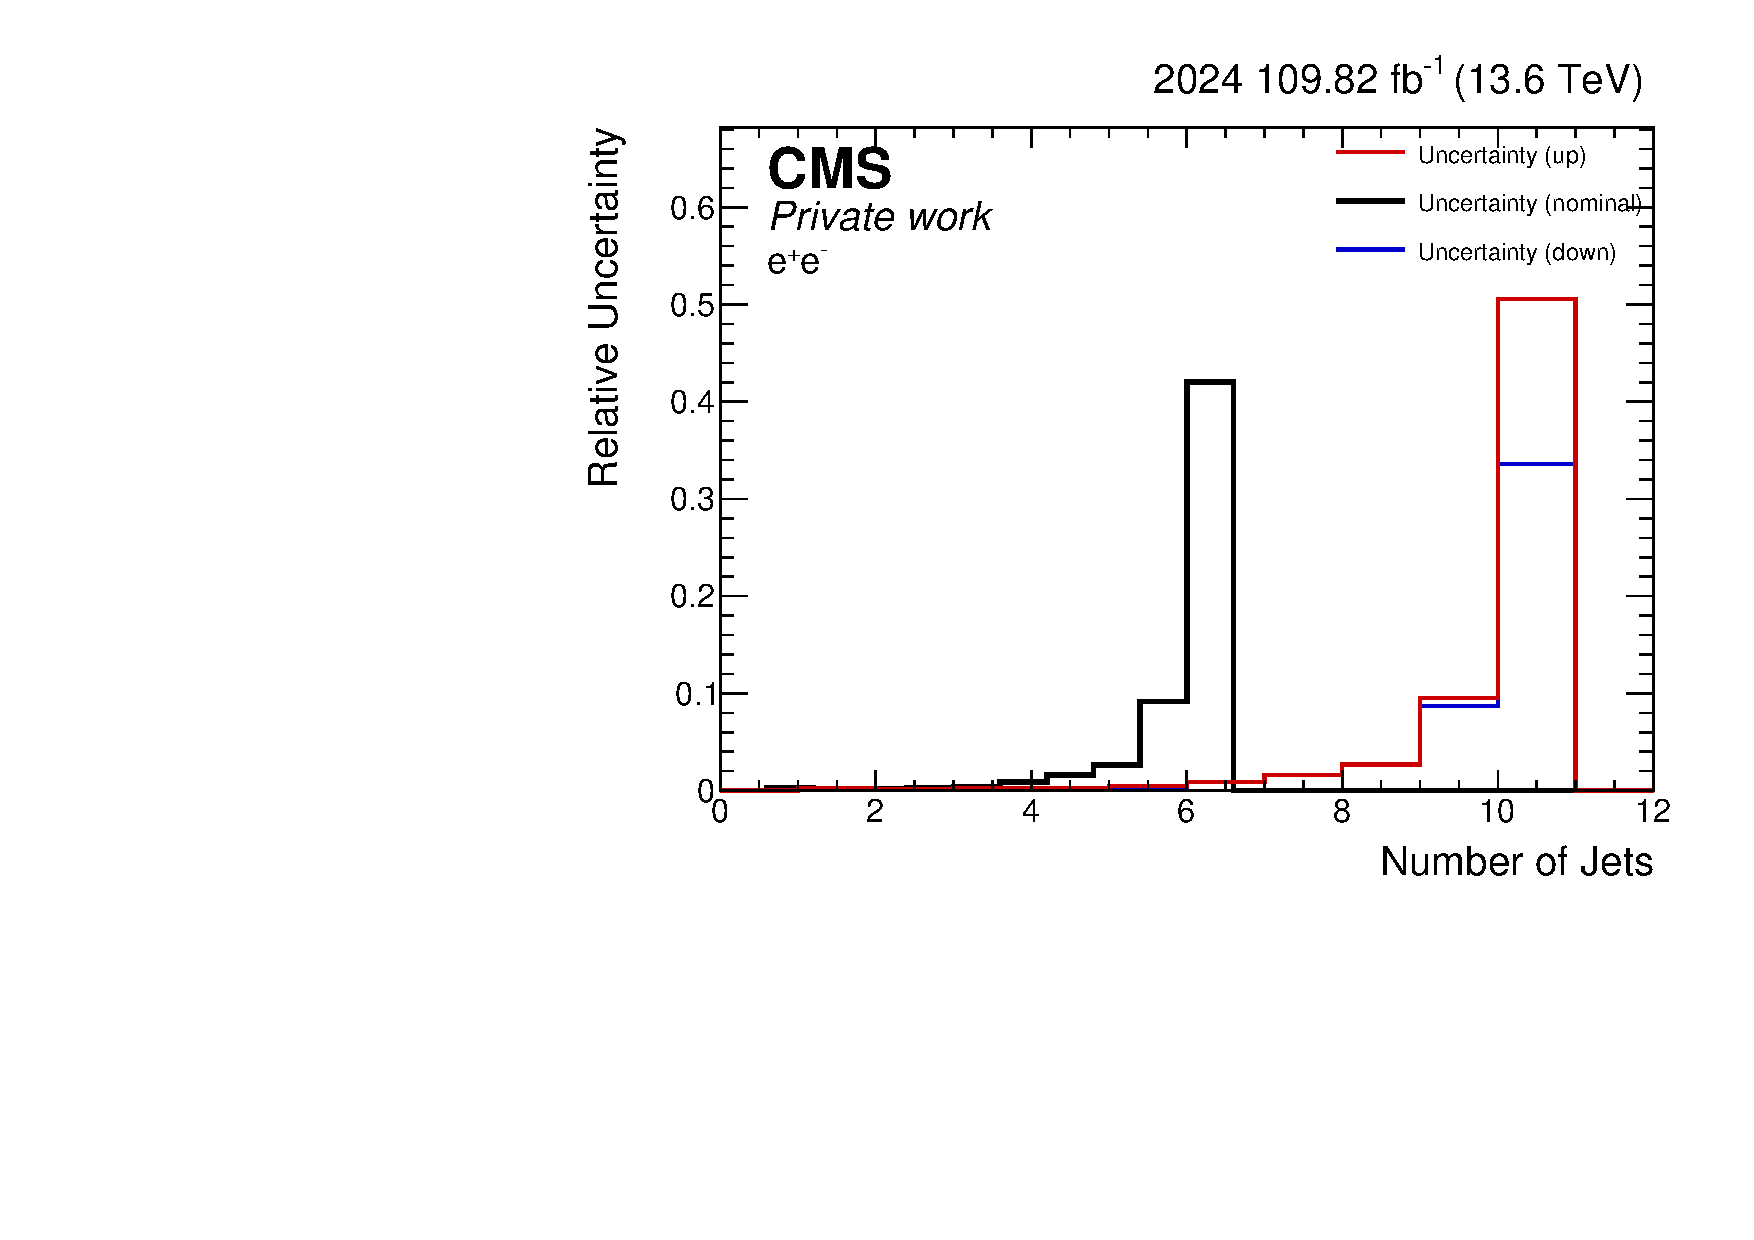
\includegraphics[width=0.48\linewidth]{figures/2024/ElEl/Statistical_Uncertainty/UncRatio_Num_Jets.pdf}
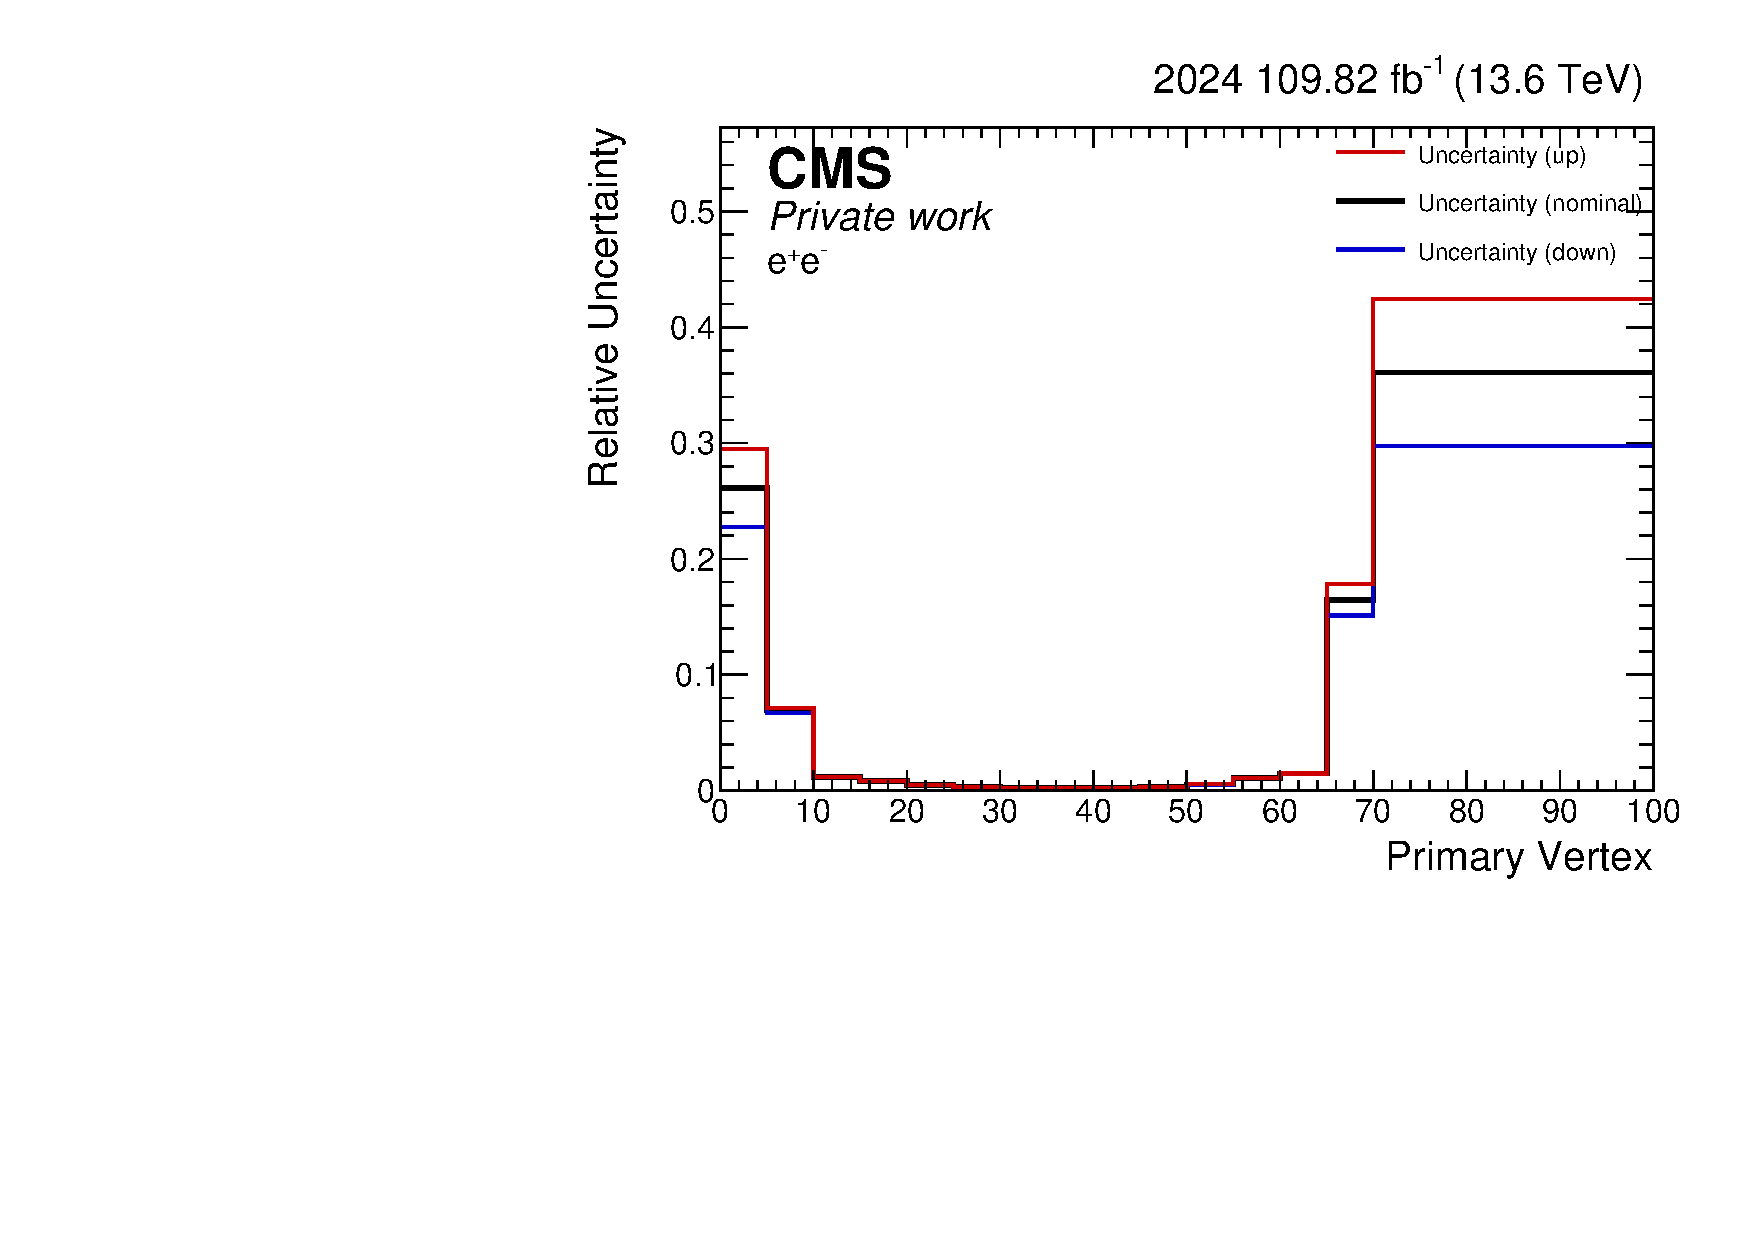
\includegraphics[width=0.48\linewidth]{figures/2024/ElEl/Statistical_Uncertainty/UncRatio_Num_PV.pdf}
\caption{Relative statistical uncertainty diagnostics, retaining the nominal, upward, and downward curves of the supplied production in the $ee$ channel. Left and right: jet and primary-vertex multiplicities.}\label{fig:extra-ElEl-Statistical-Uncertainty-Num_Jets}\end{figure}
\begin{figure}[p]\centering
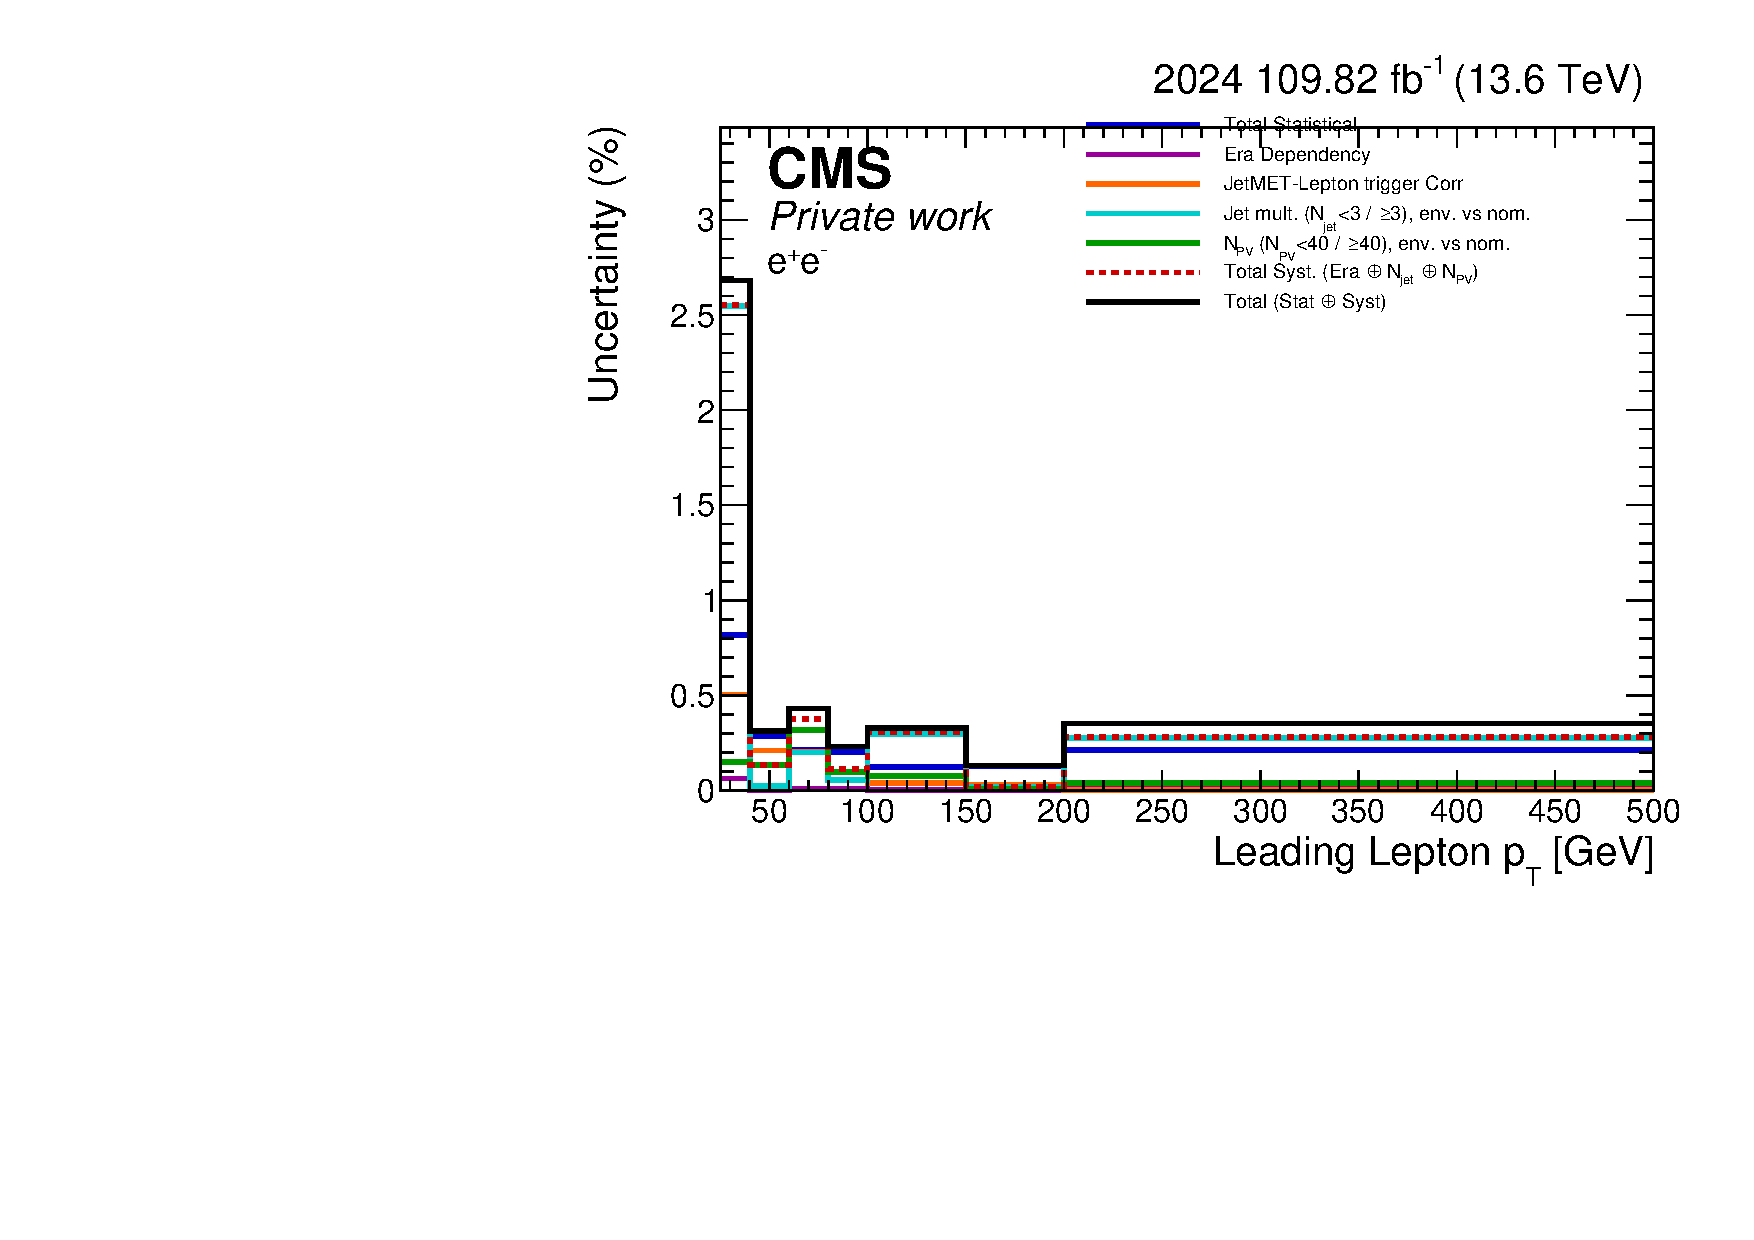
\includegraphics[width=0.48\linewidth]{figures/2024/ElEl/Uncertainty_Breakdown/Breakdown_Lep1pt.pdf}
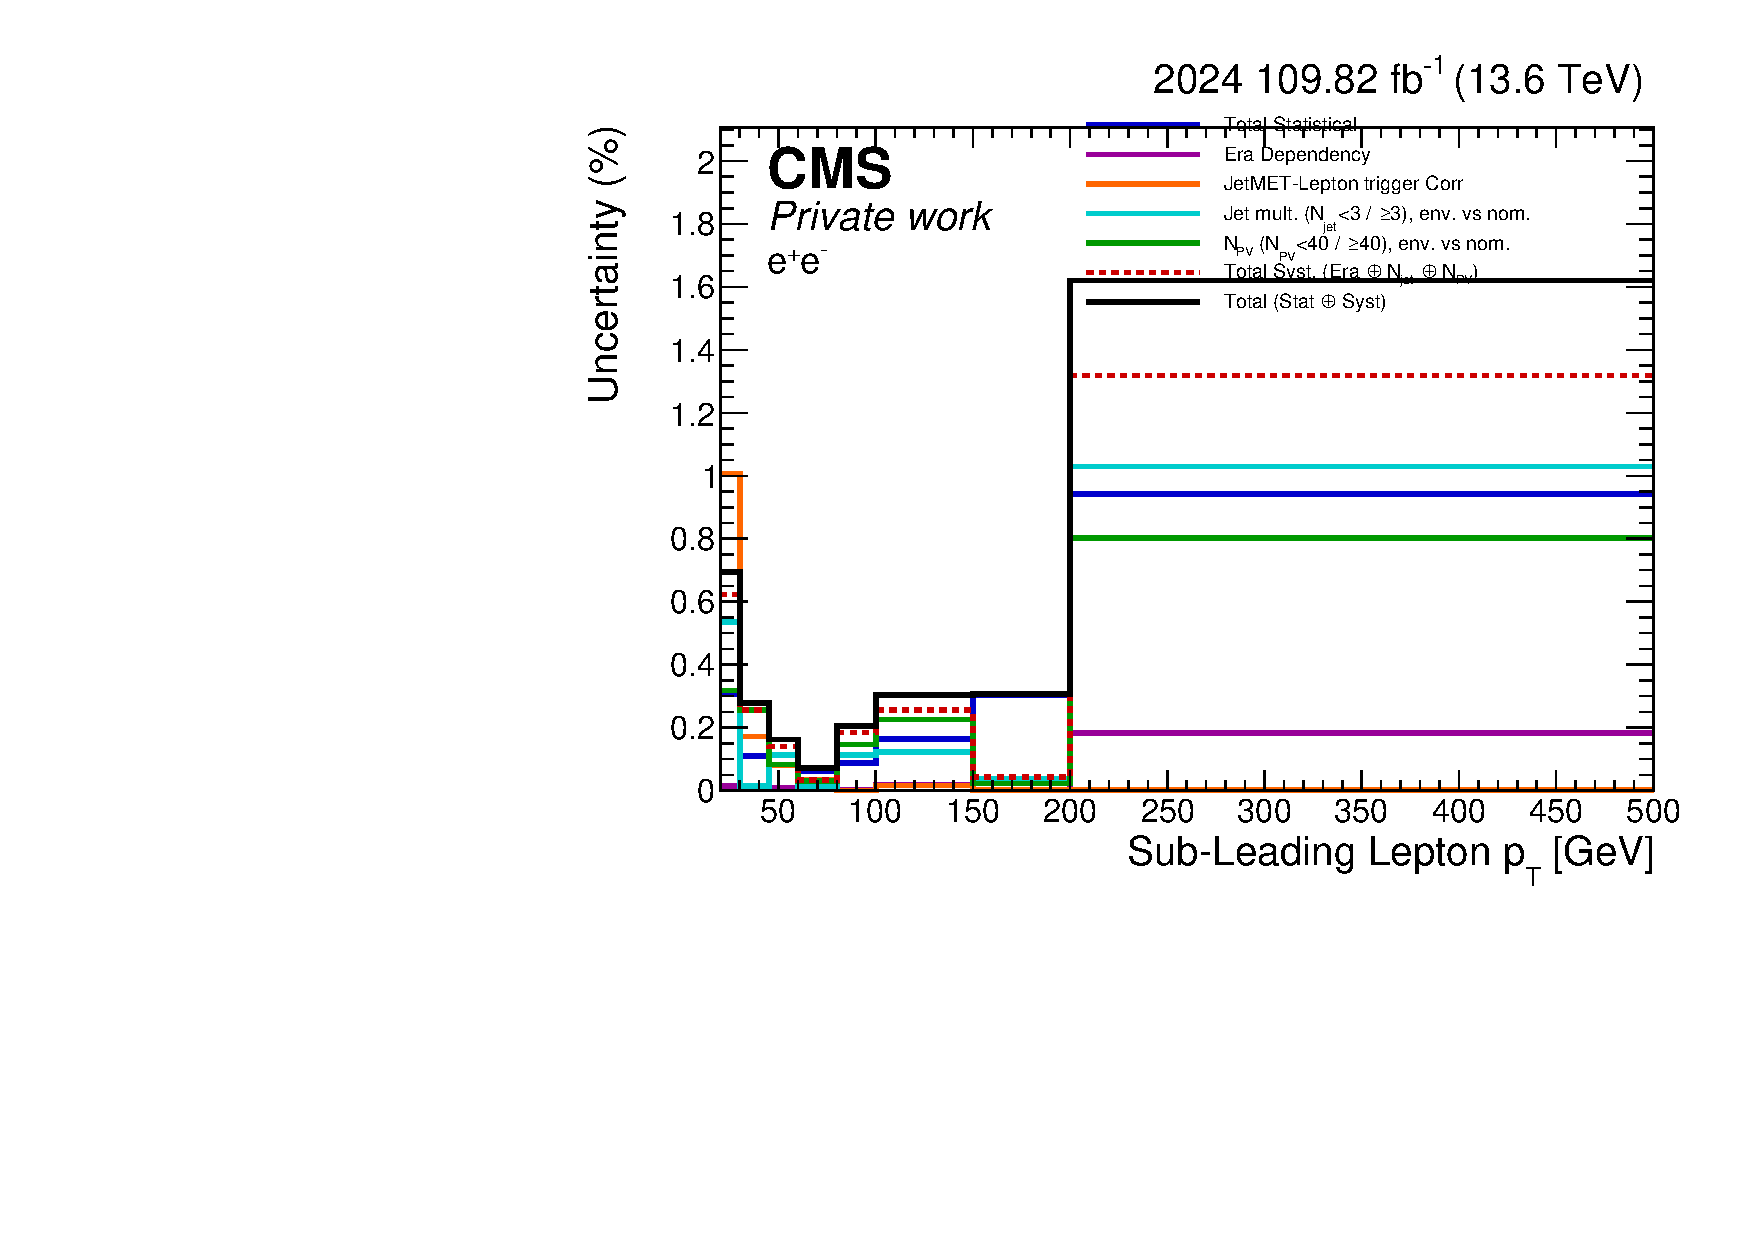
\includegraphics[width=0.48\linewidth]{figures/2024/ElEl/Uncertainty_Breakdown/Breakdown_Lep2pt.pdf}
\caption{Absolute uncertainty component breakdown in the $ee$ channel. Left and right: leading and subleading lepton $p_{\mathrm{T}}$.}\label{fig:extra-ElEl-Uncertainty-Breakdown-Lep1pt}\end{figure}
\begin{figure}[p]\centering
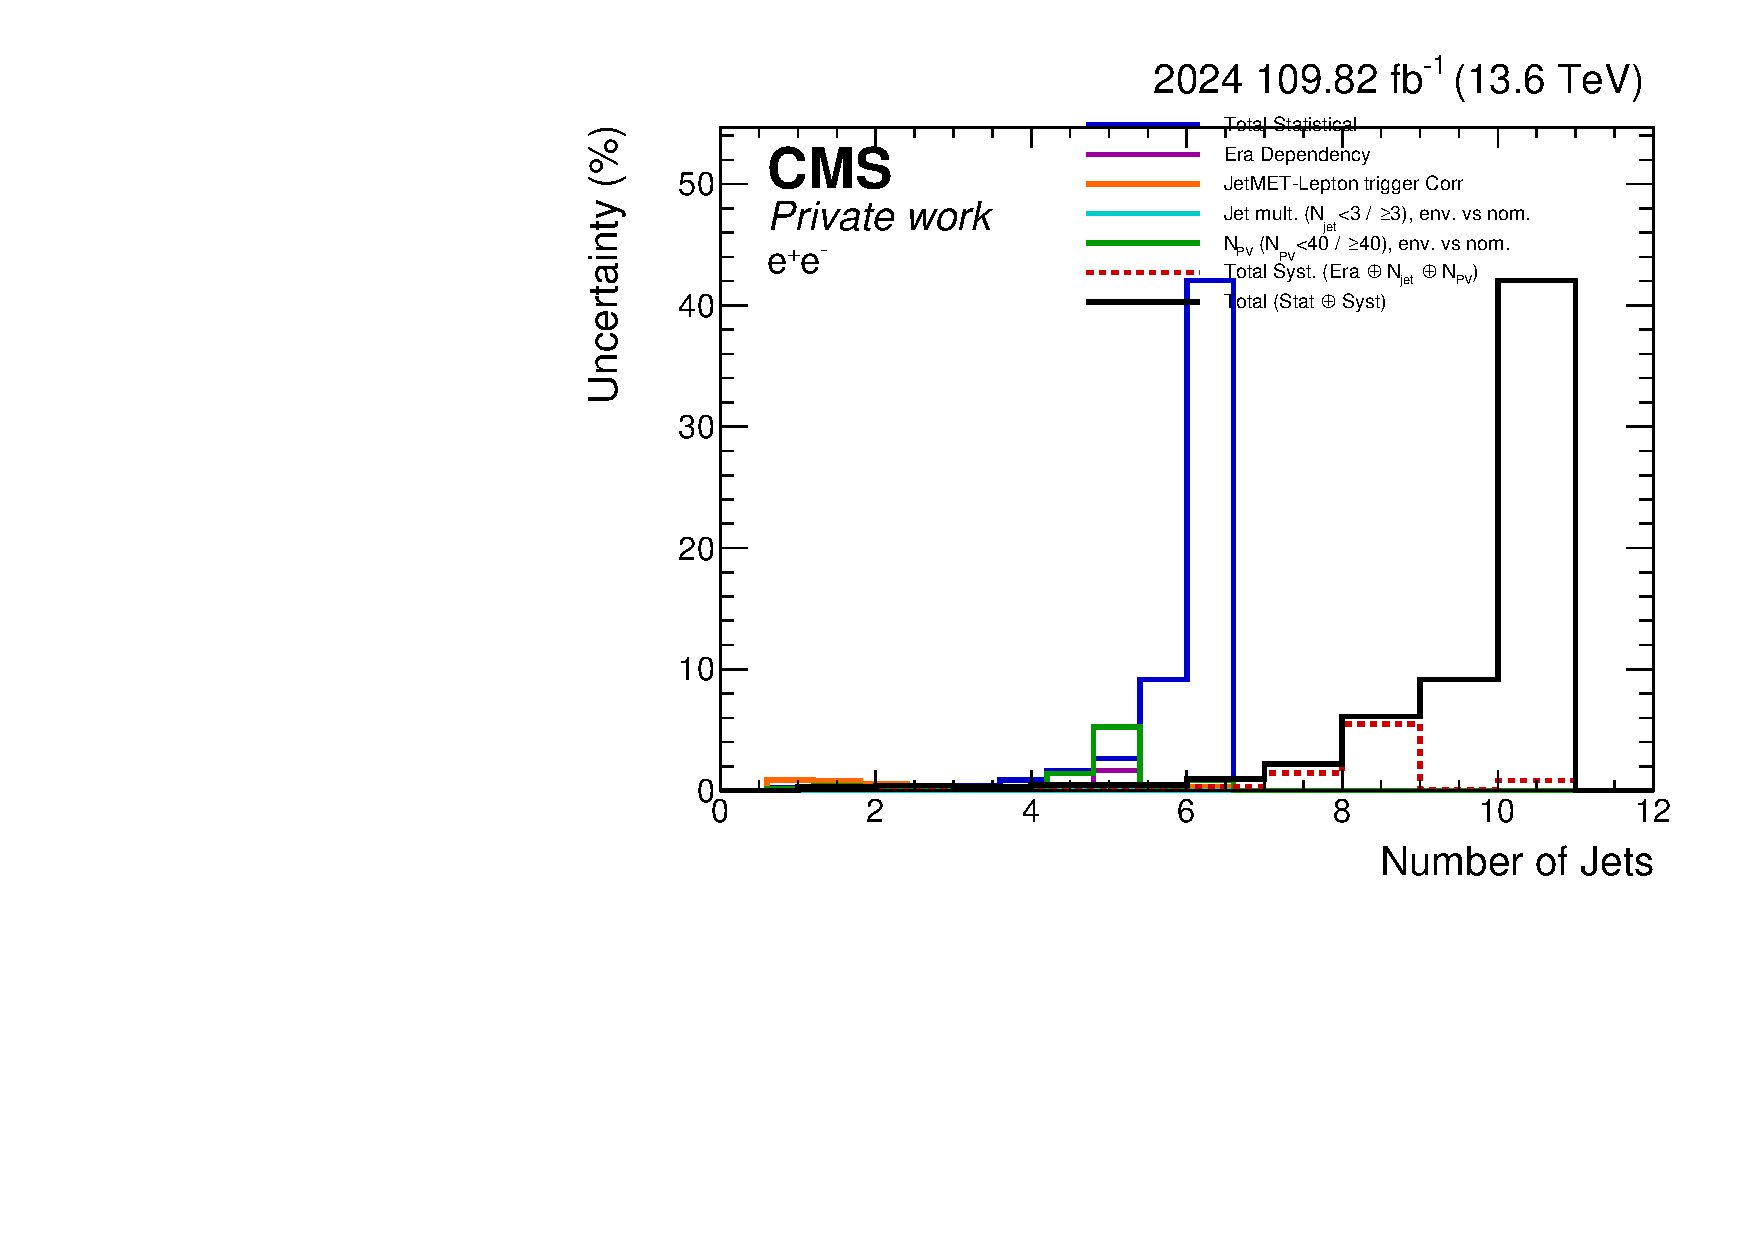
\includegraphics[width=0.48\linewidth]{figures/2024/ElEl/Uncertainty_Breakdown/Breakdown_Num_Jets.pdf}
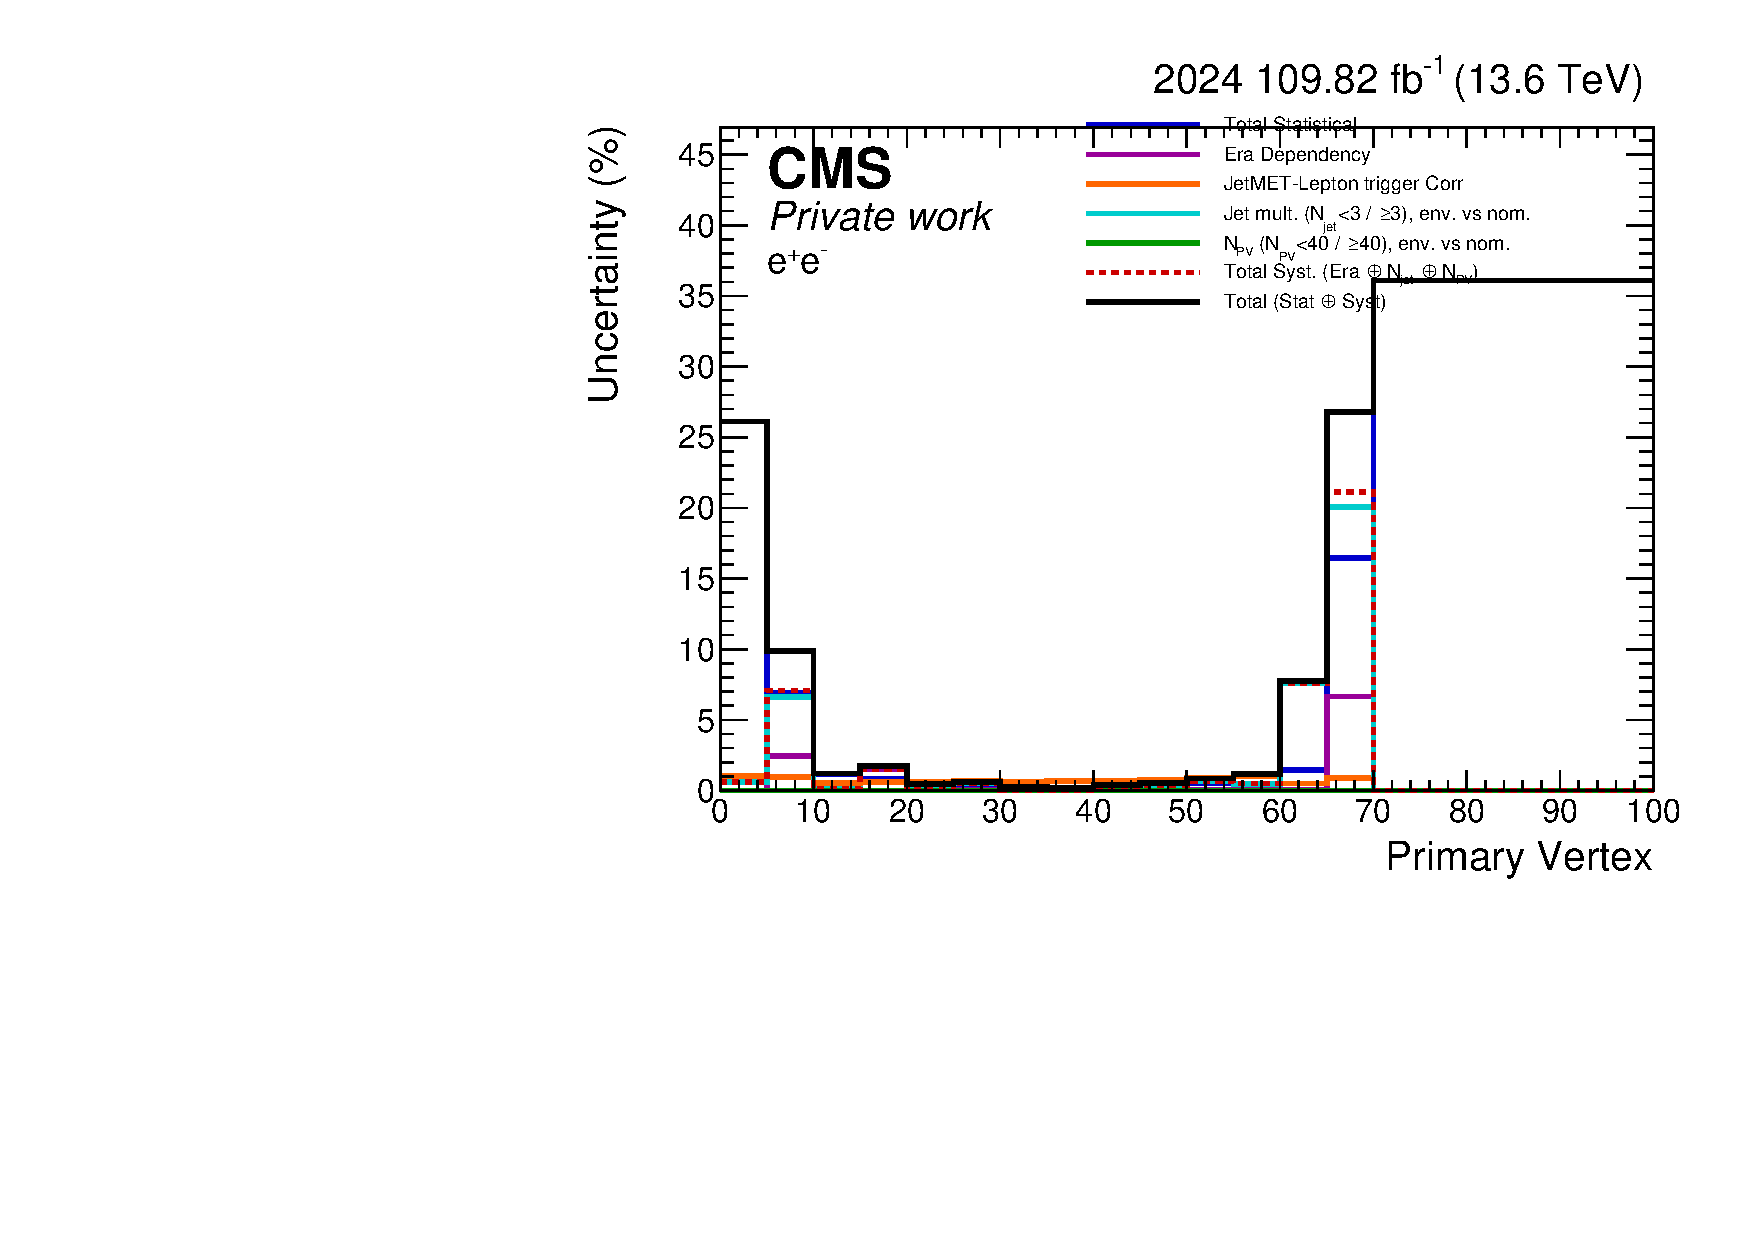
\includegraphics[width=0.48\linewidth]{figures/2024/ElEl/Uncertainty_Breakdown/Breakdown_Num_PV.pdf}
\caption{Absolute uncertainty component breakdown in the $ee$ channel. Left and right: jet and primary-vertex multiplicities.}\label{fig:extra-ElEl-Uncertainty-Breakdown-Num_Jets}\end{figure}
\begin{figure}[p]\centering
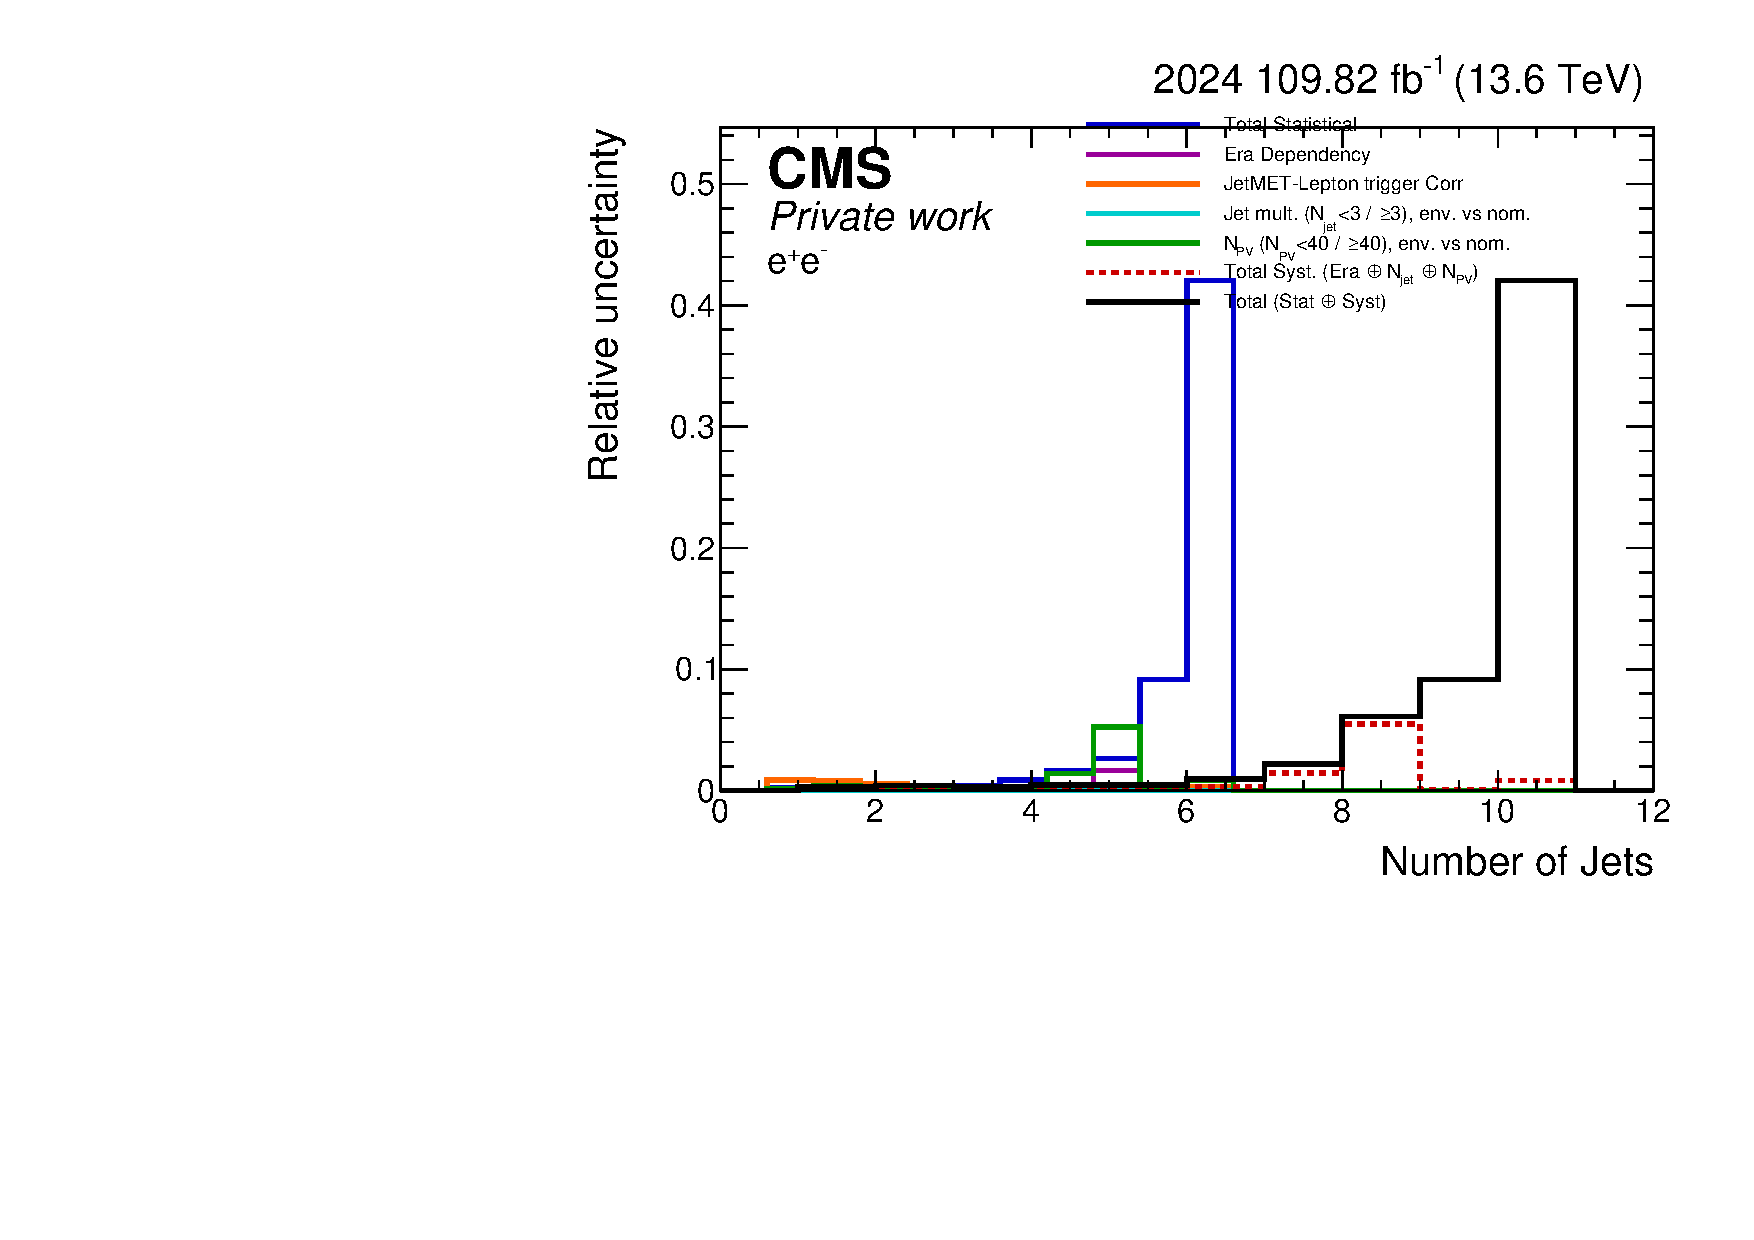
\includegraphics[width=0.48\linewidth]{figures/2024/ElEl/Relative_Uncertainty_Breakdown/Breakdown_Num_Jets.pdf}
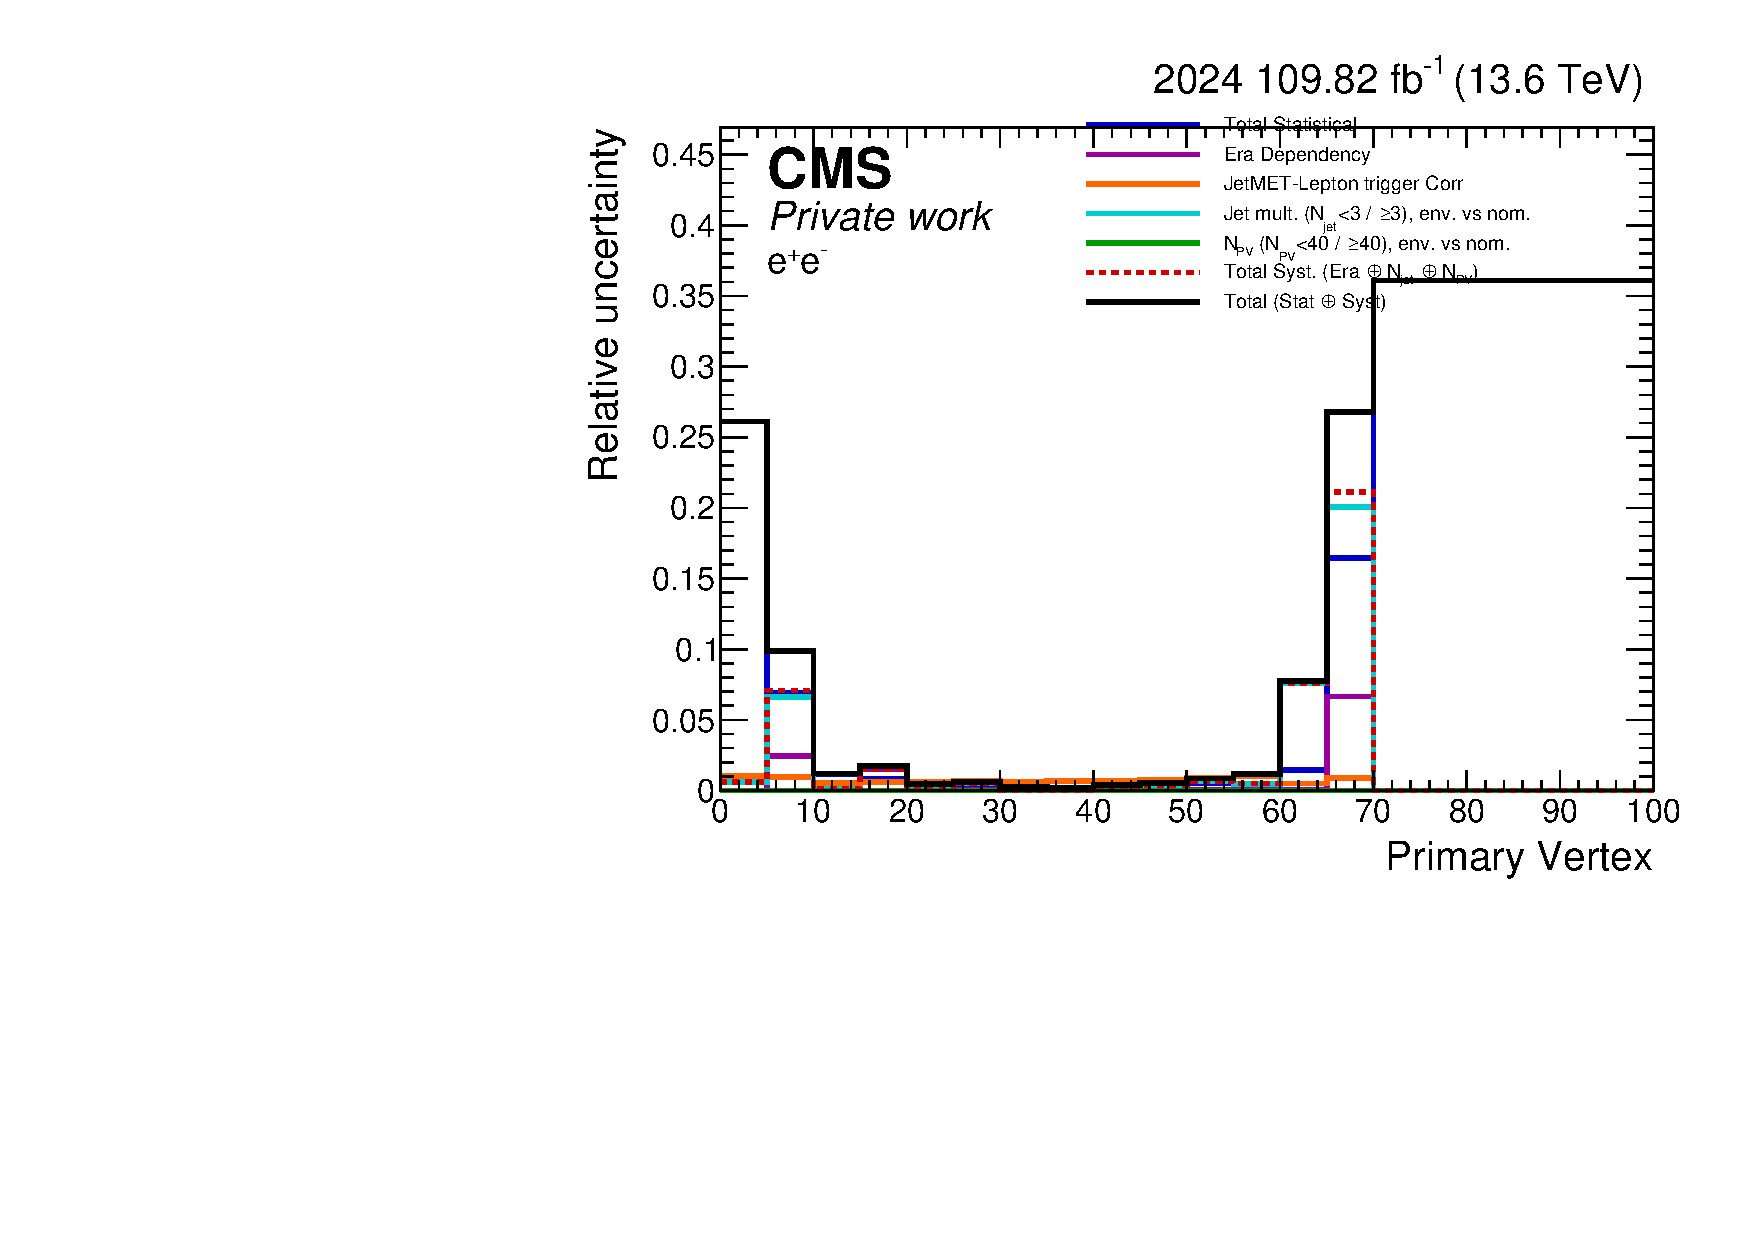
\includegraphics[width=0.48\linewidth]{figures/2024/ElEl/Relative_Uncertainty_Breakdown/Breakdown_Num_PV.pdf}
\caption{Relative uncertainty component breakdown versus event activity in the $ee$ channel. Left and right: jet and primary-vertex multiplicities.}\label{fig:extra-ElEl-Relative-Uncertainty-Breakdown-Num_Jets}\end{figure}
\begin{figure}[p]\centering
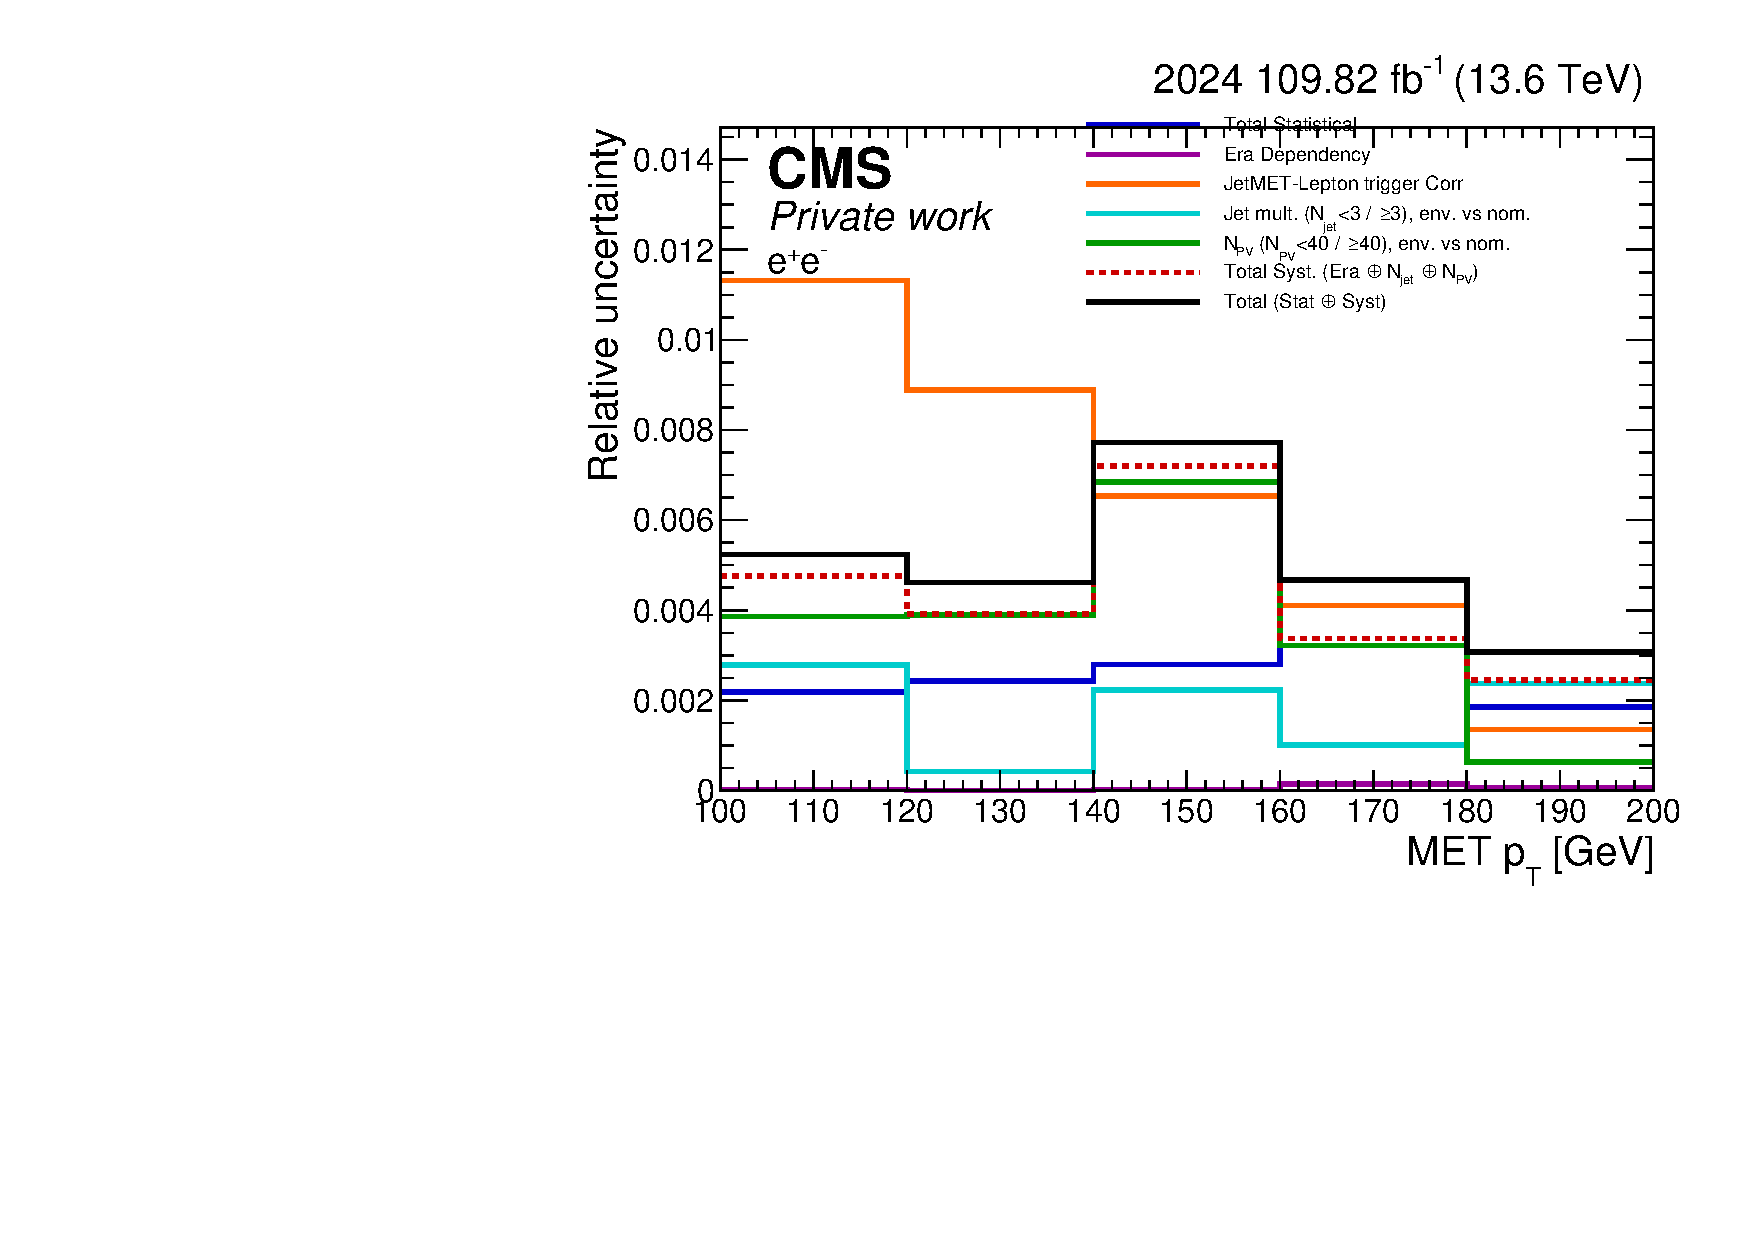
\includegraphics[width=0.48\linewidth]{figures/2024/ElEl/Relative_Uncertainty_Breakdown/Breakdown_METpt.pdf}
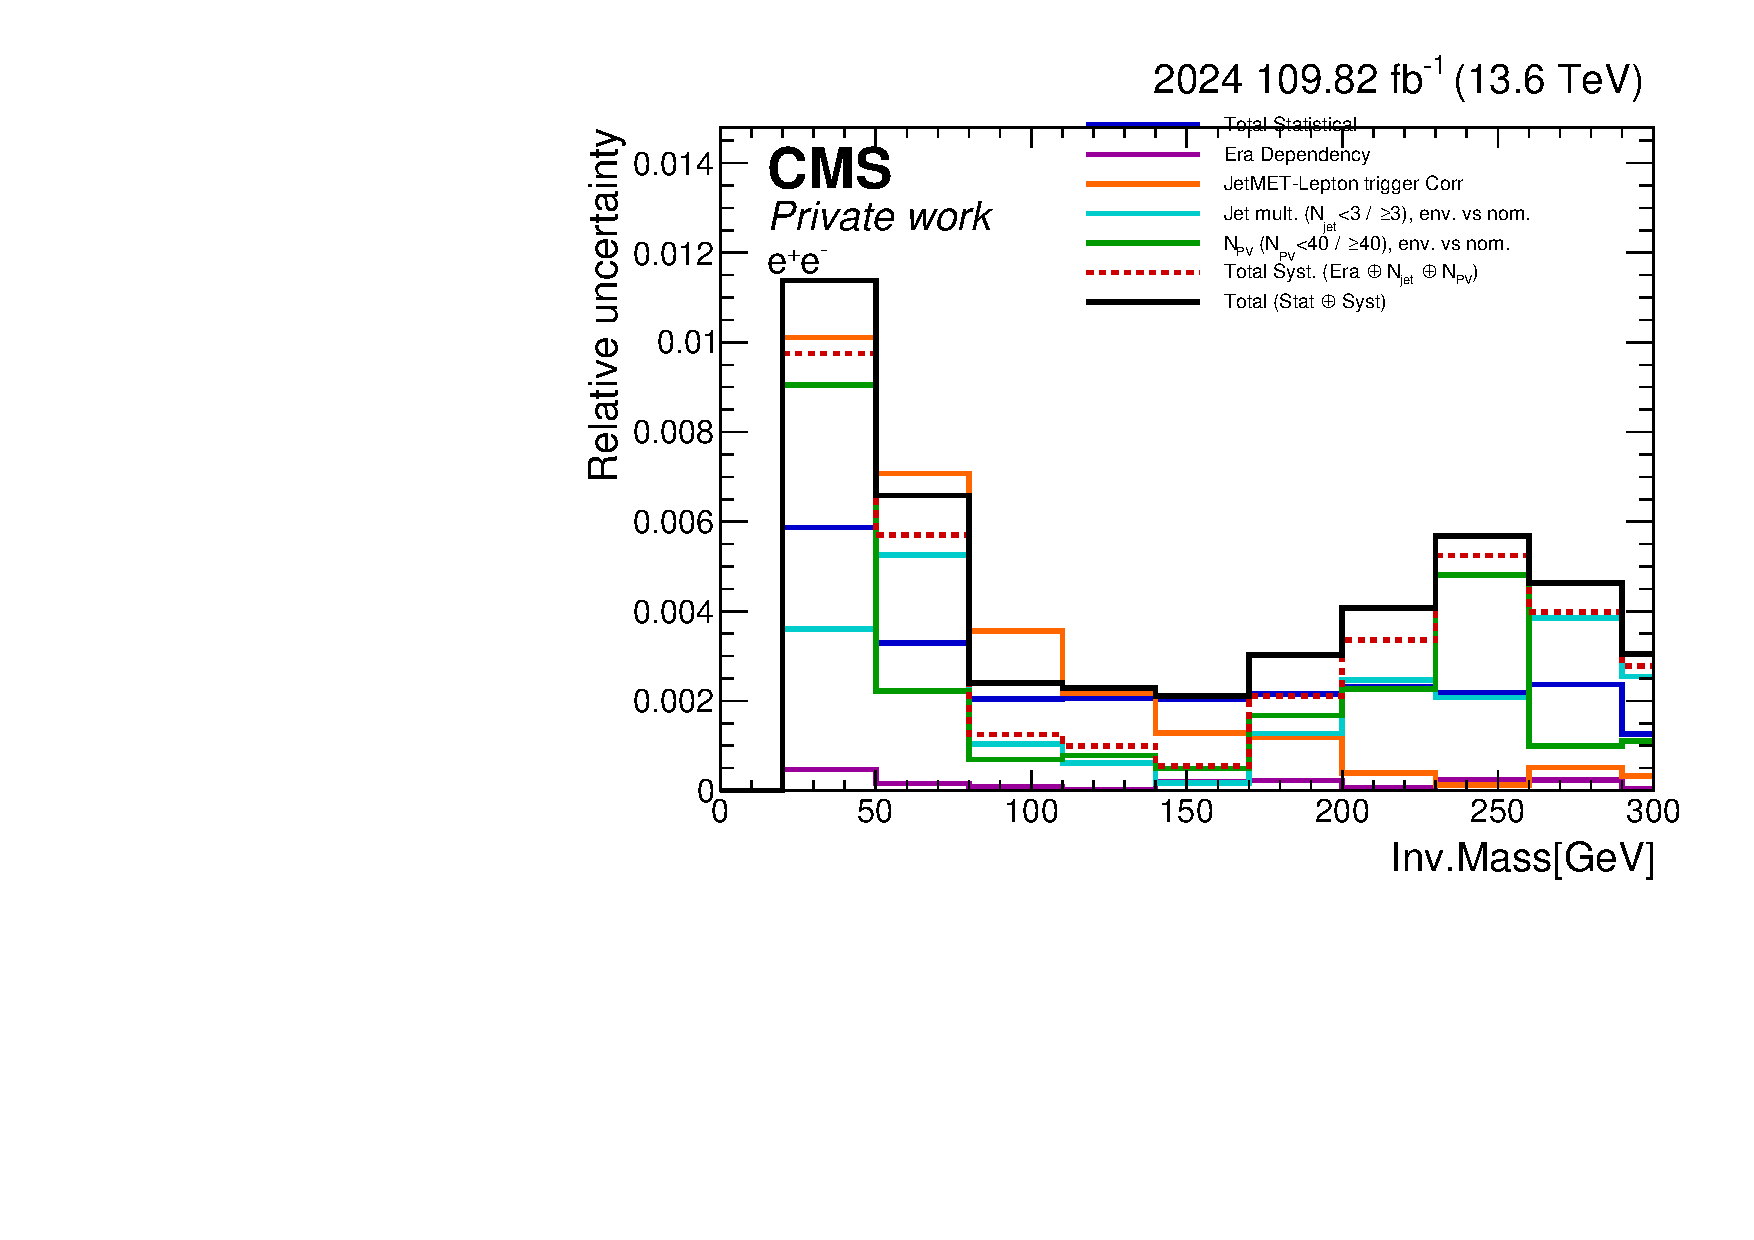
\includegraphics[width=0.48\linewidth]{figures/2024/ElEl/Relative_Uncertainty_Breakdown/Breakdown_DiLepMass.pdf}
\caption{Relative uncertainty component breakdown versus event kinematics in the $ee$ channel. Left and right: missing transverse momentum and dilepton invariant mass.}\label{fig:extra-ElEl-Relative-Uncertainty-Breakdown-METpt}\end{figure}
\begin{figure}[p]\centering
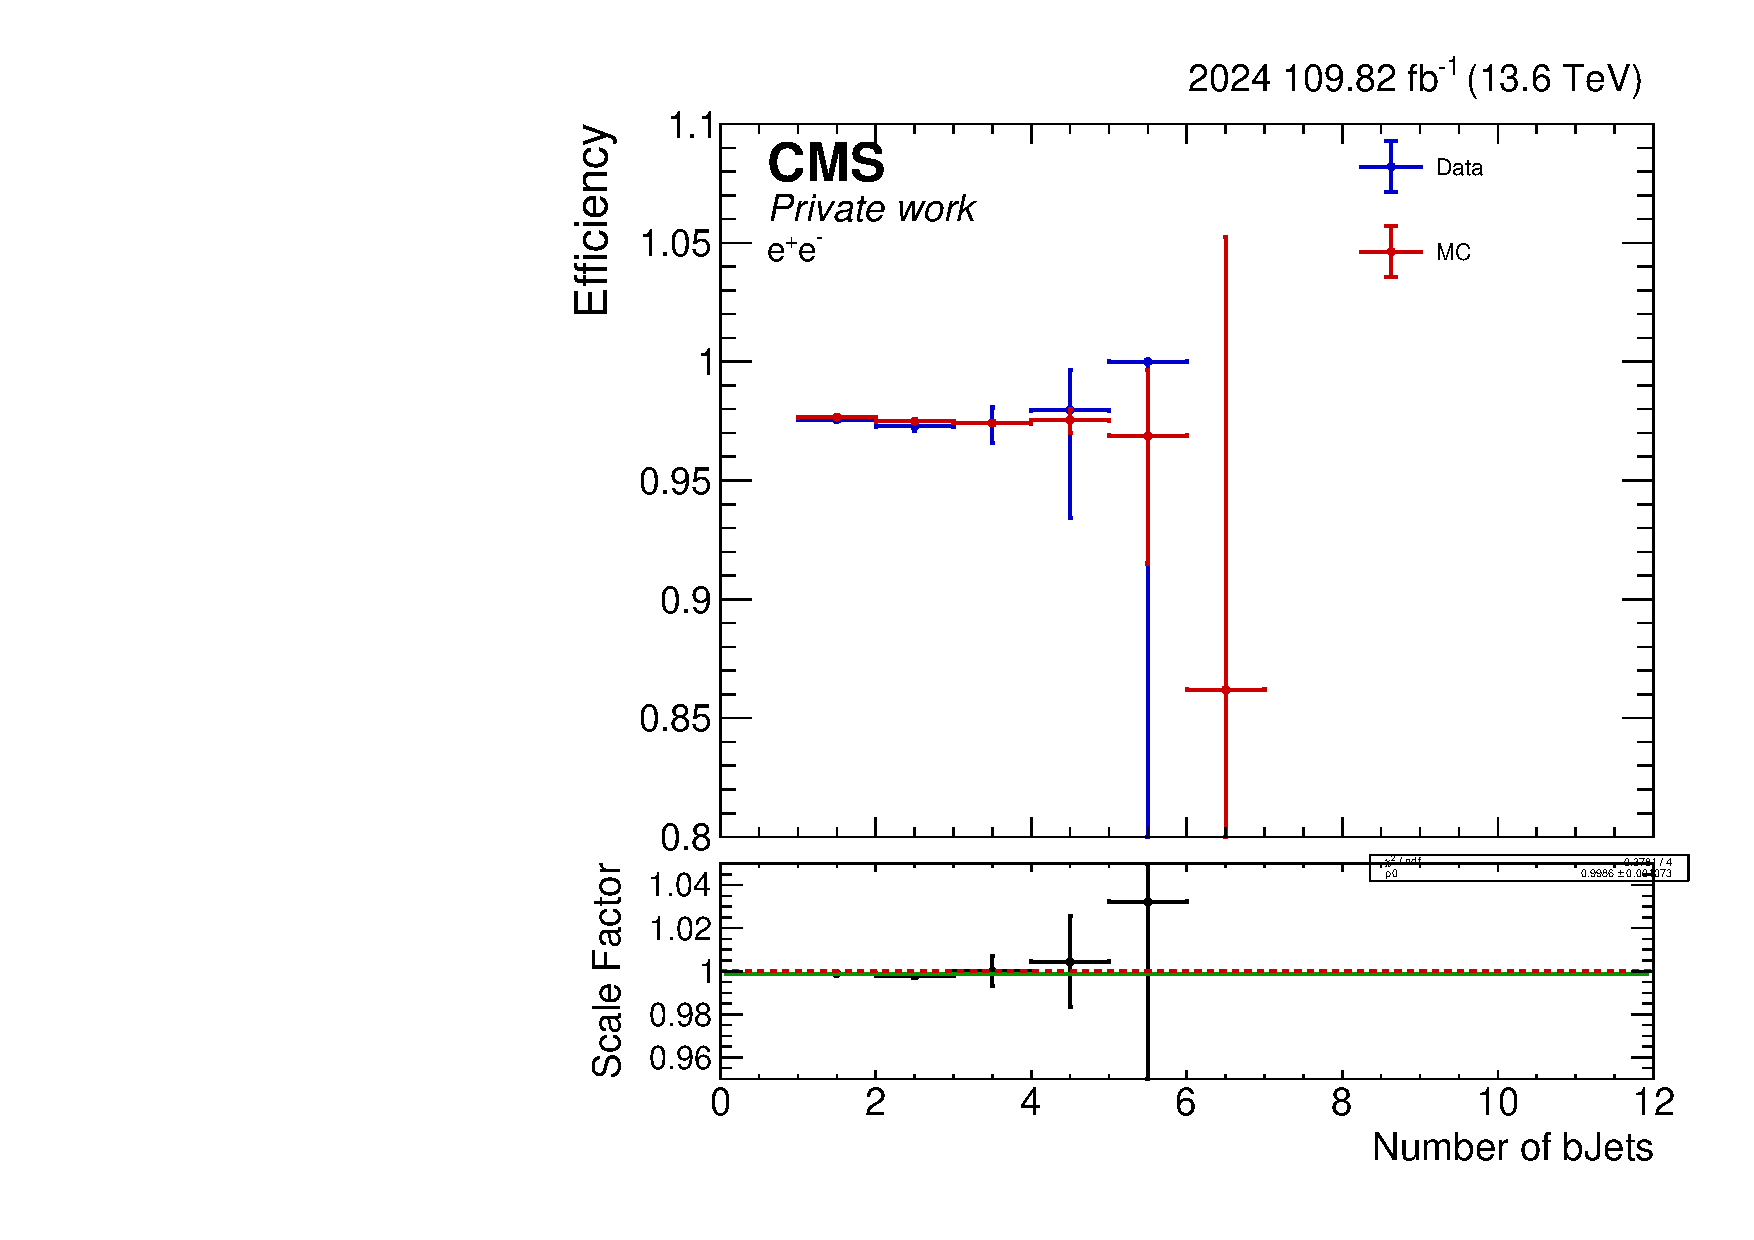
\includegraphics[width=0.48\linewidth]{figures/2024/ElEl/ScaleFactor/SF_Num_bJets.pdf}
\caption{Efficiency comparison and scale factor versus heavy-flavour activity in the $ee$ channel. $b$-tagged jet multiplicity.}\label{fig:extra-ElEl-ScaleFactor-Num_bJets}\end{figure}
\clearpage\subsection{$e\mu$ channel}
\begin{figure}[p]\centering
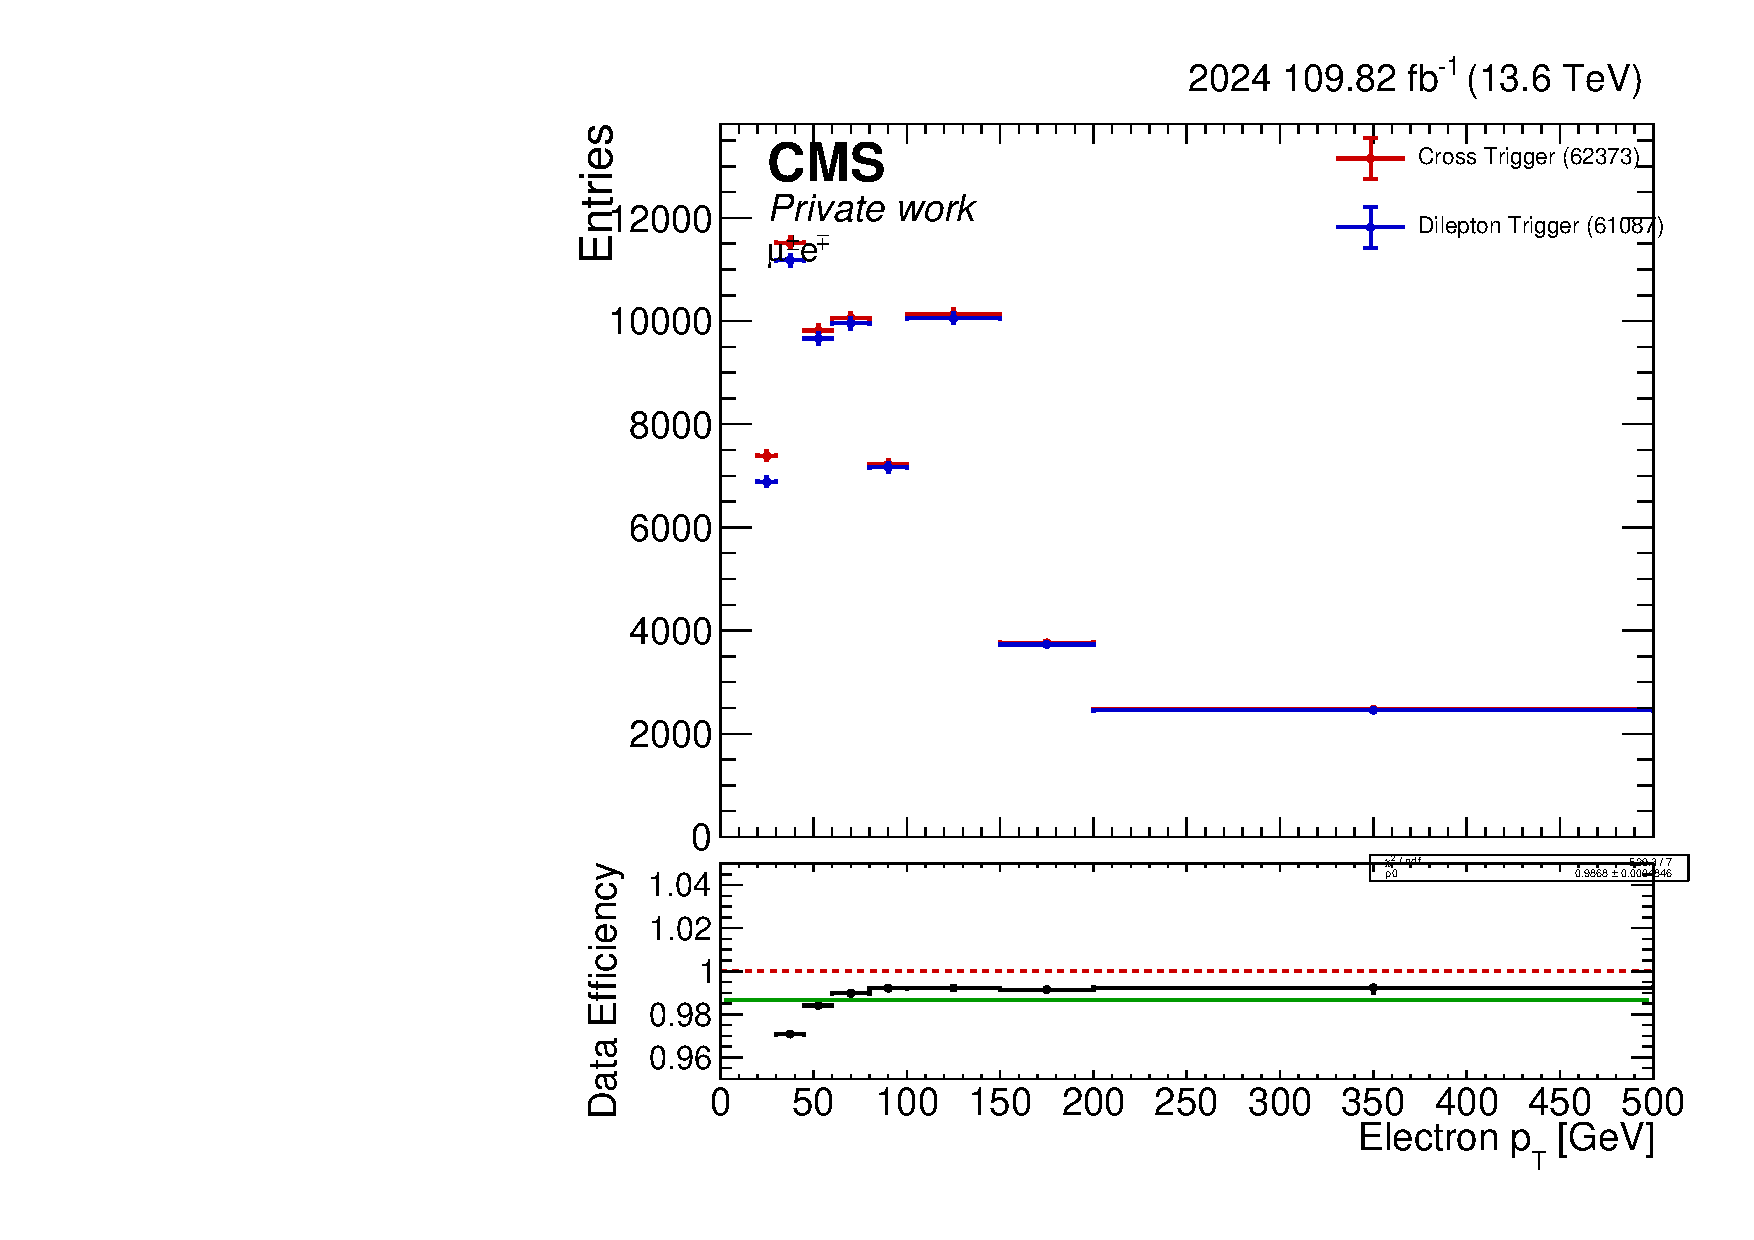
\includegraphics[width=0.48\linewidth]{figures/2024/MuEl/TrigEffData/TrigEff_ElPt.pdf}
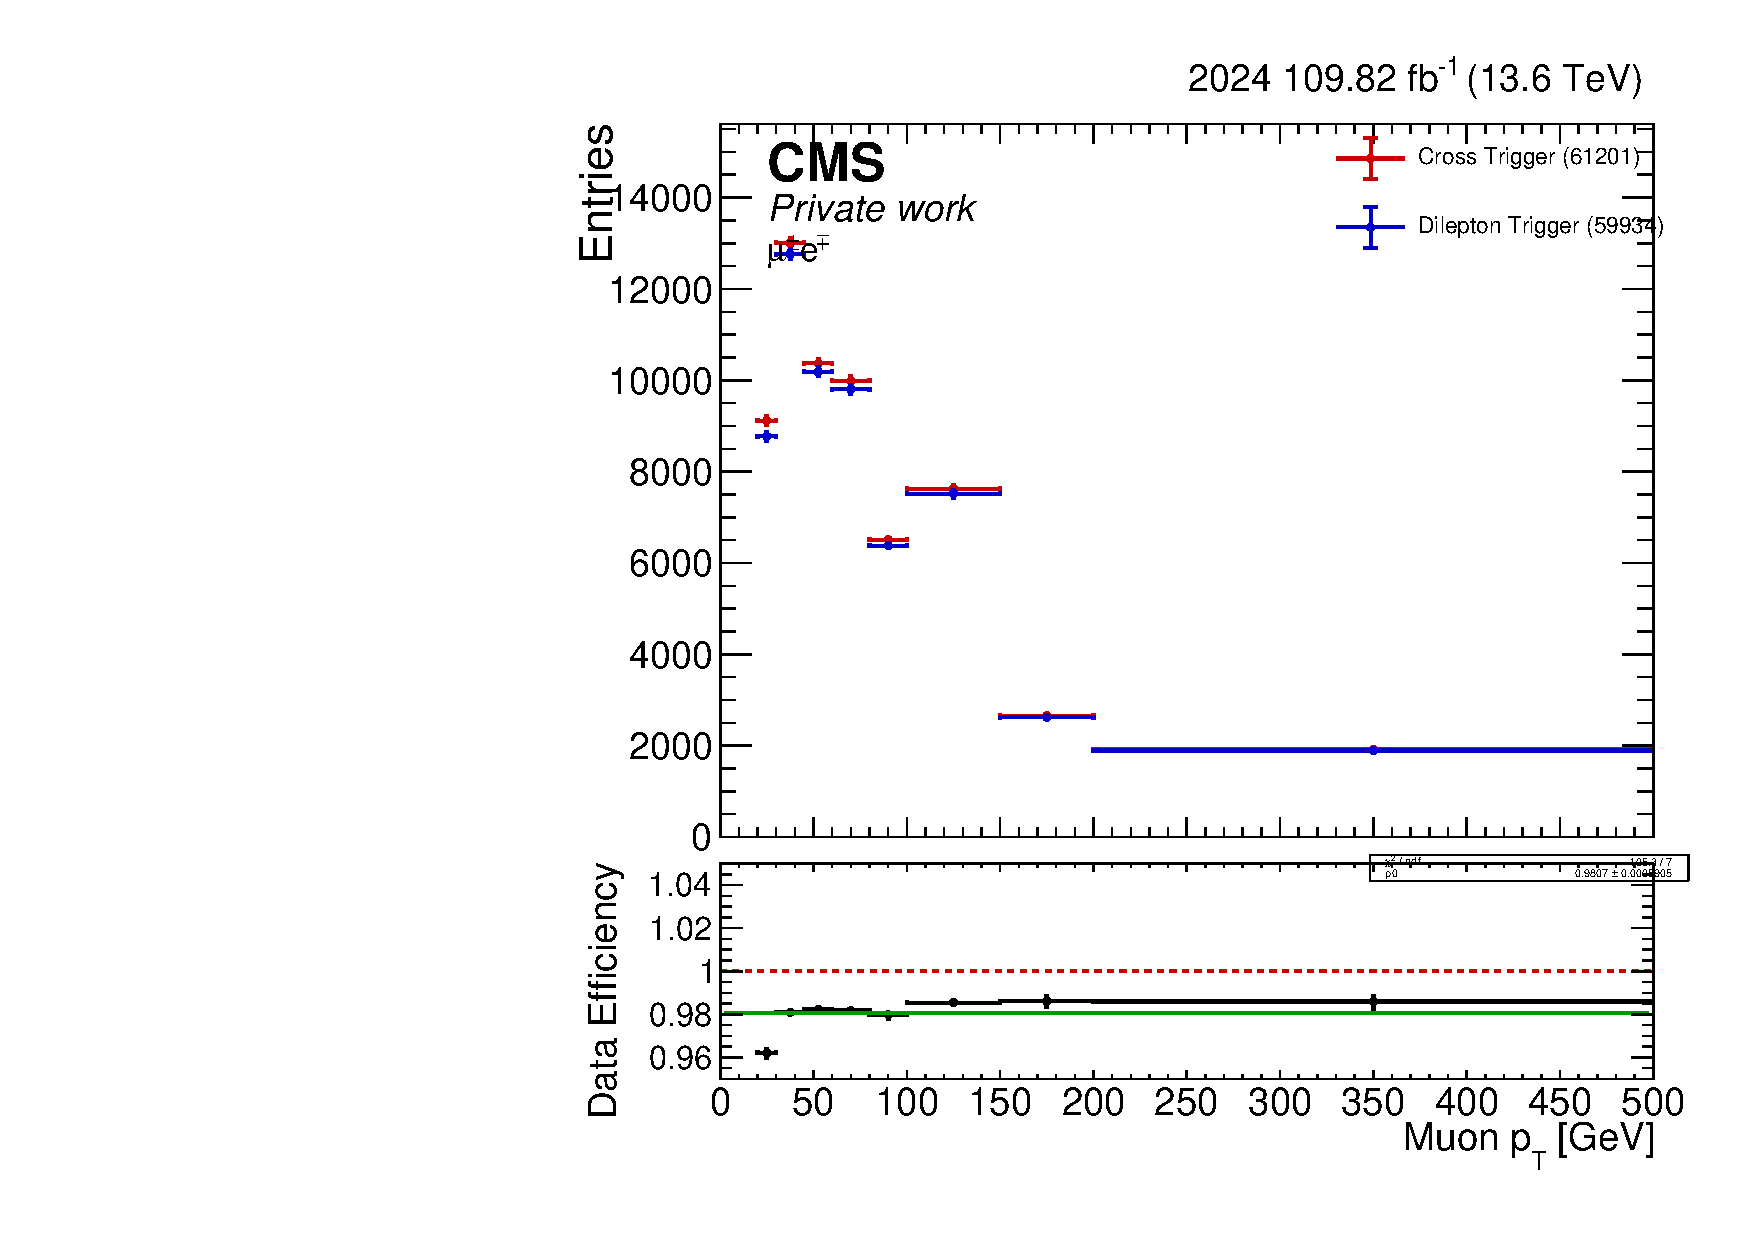
\includegraphics[width=0.48\linewidth]{figures/2024/MuEl/TrigEffData/TrigEff_MuPt.pdf}
\caption{Data trigger numerator and reference-sample distributions (upper panels), with their efficiency ratios (lower panels) in the $e\mu$ channel. Left and right: electron and muon $p_{\mathrm{T}}$.}\label{fig:extra-MuEl-TrigEffData-ElPt}\end{figure}
\begin{figure}[p]\centering
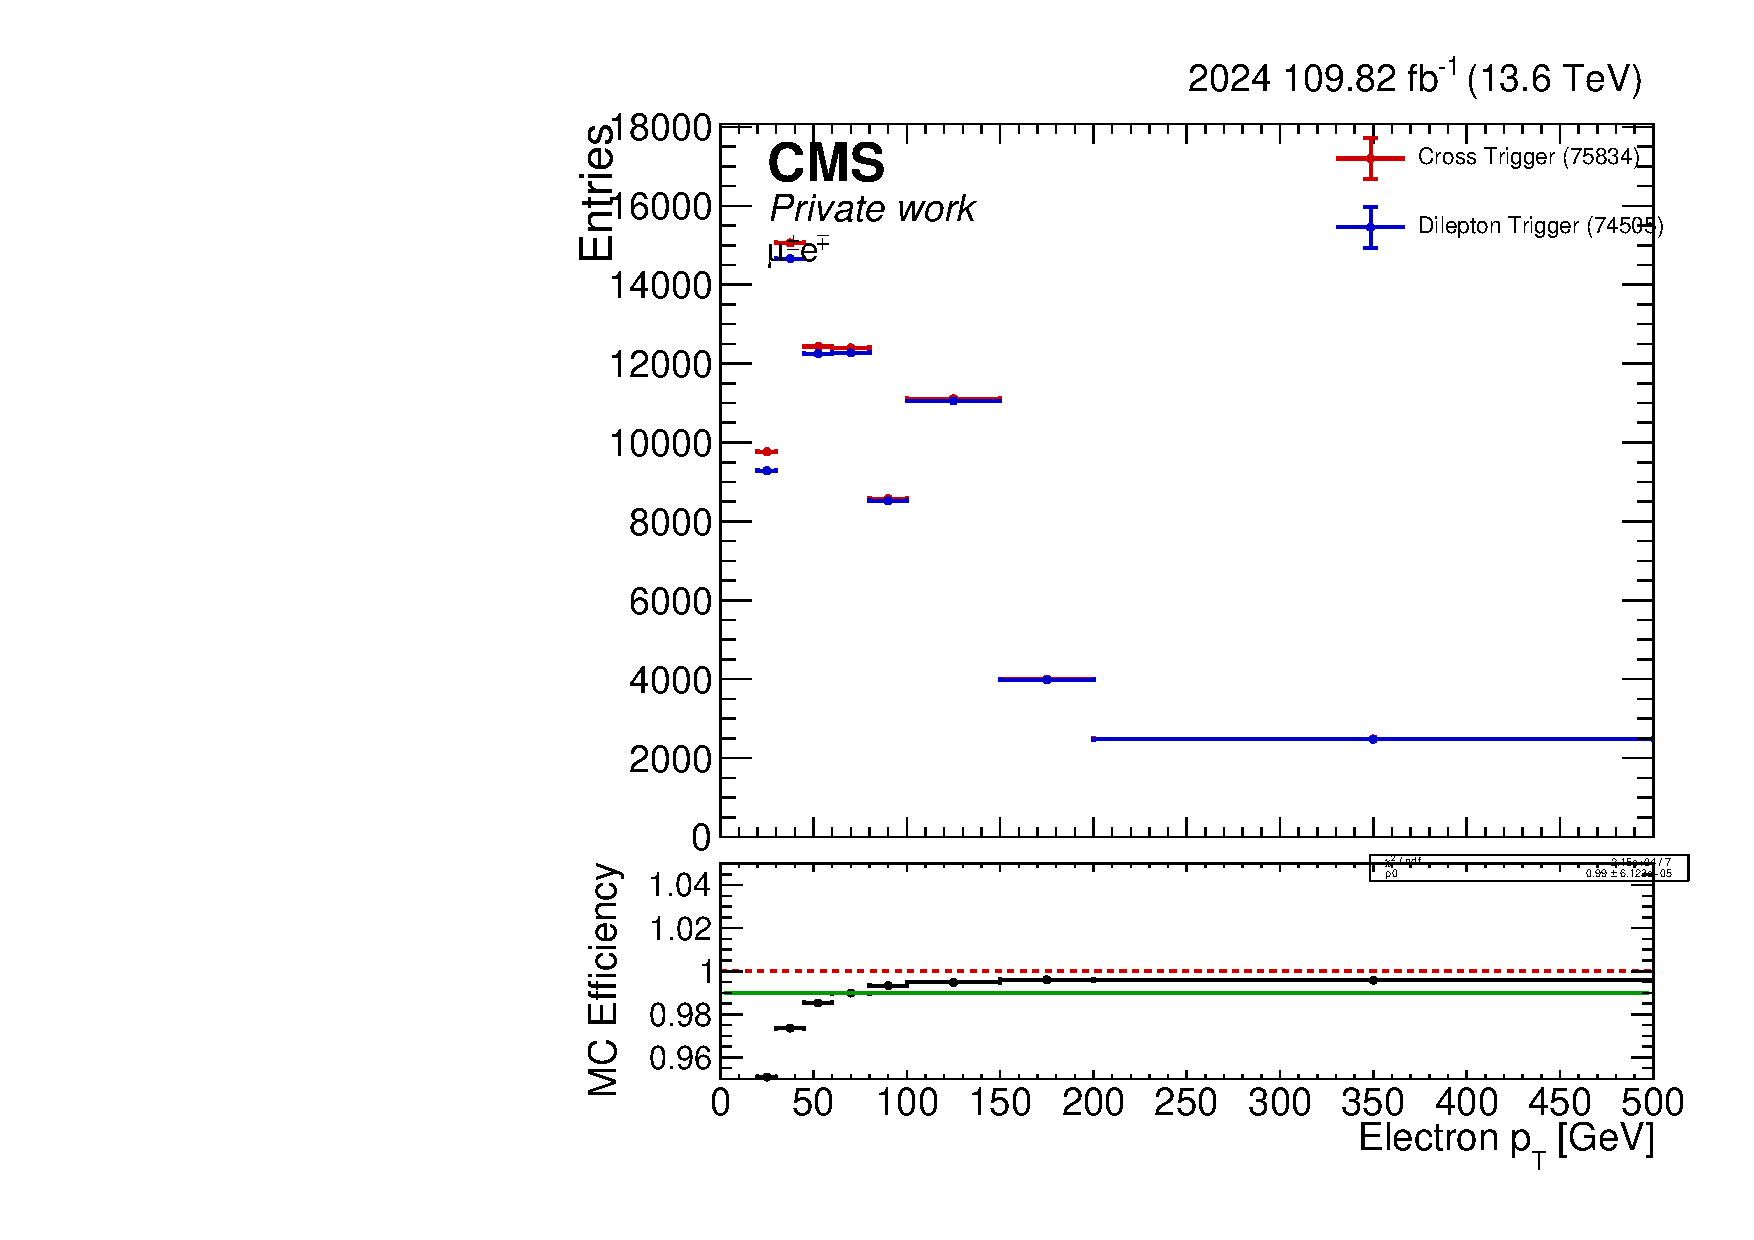
\includegraphics[width=0.48\linewidth]{figures/2024/MuEl/TrigEffMC/TrigEff_ElPt.pdf}
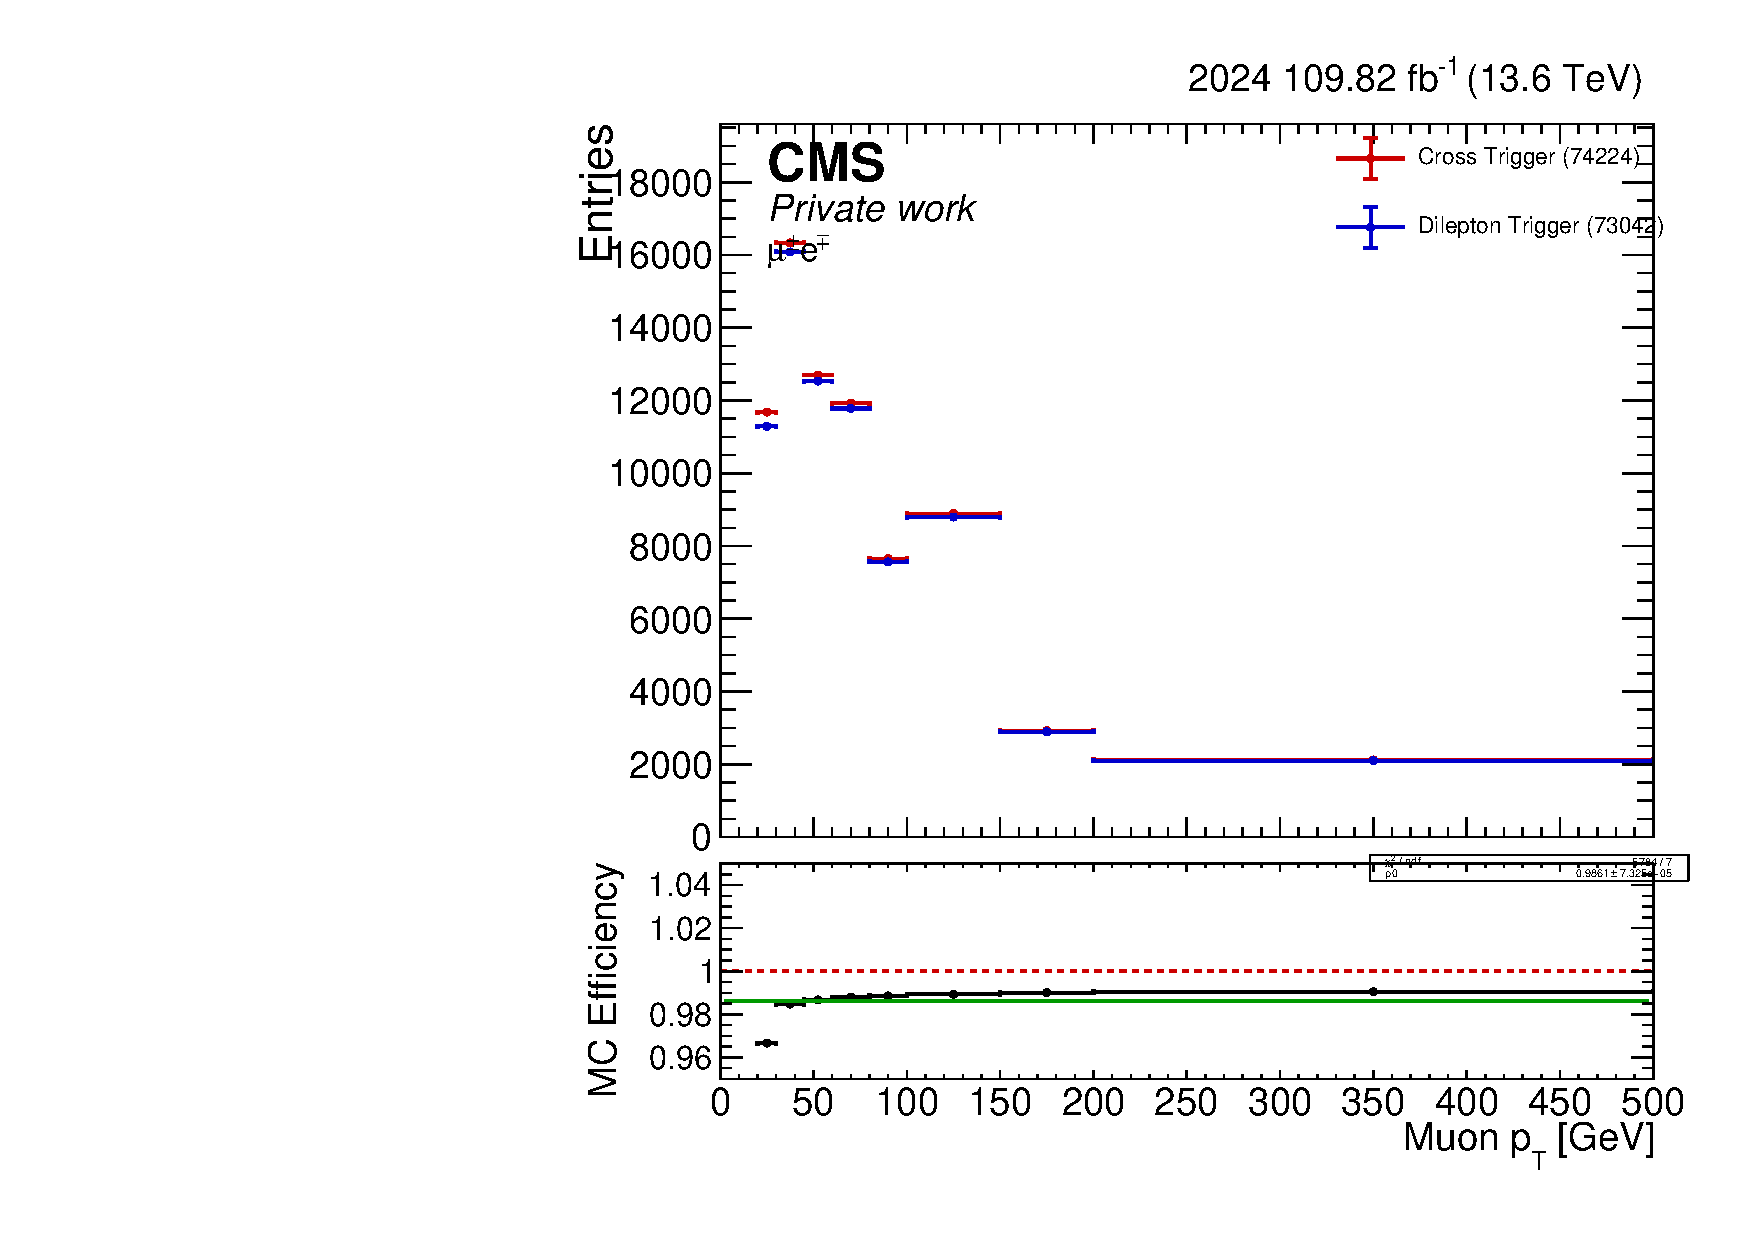
\includegraphics[width=0.48\linewidth]{figures/2024/MuEl/TrigEffMC/TrigEff_MuPt.pdf}
\caption{Simulated trigger numerator and reference-sample distributions (upper panels), with their efficiency ratios (lower panels) in the $e\mu$ channel. Left and right: electron and muon $p_{\mathrm{T}}$.}\label{fig:extra-MuEl-TrigEffMC-ElPt}\end{figure}
\begin{figure}[p]\centering
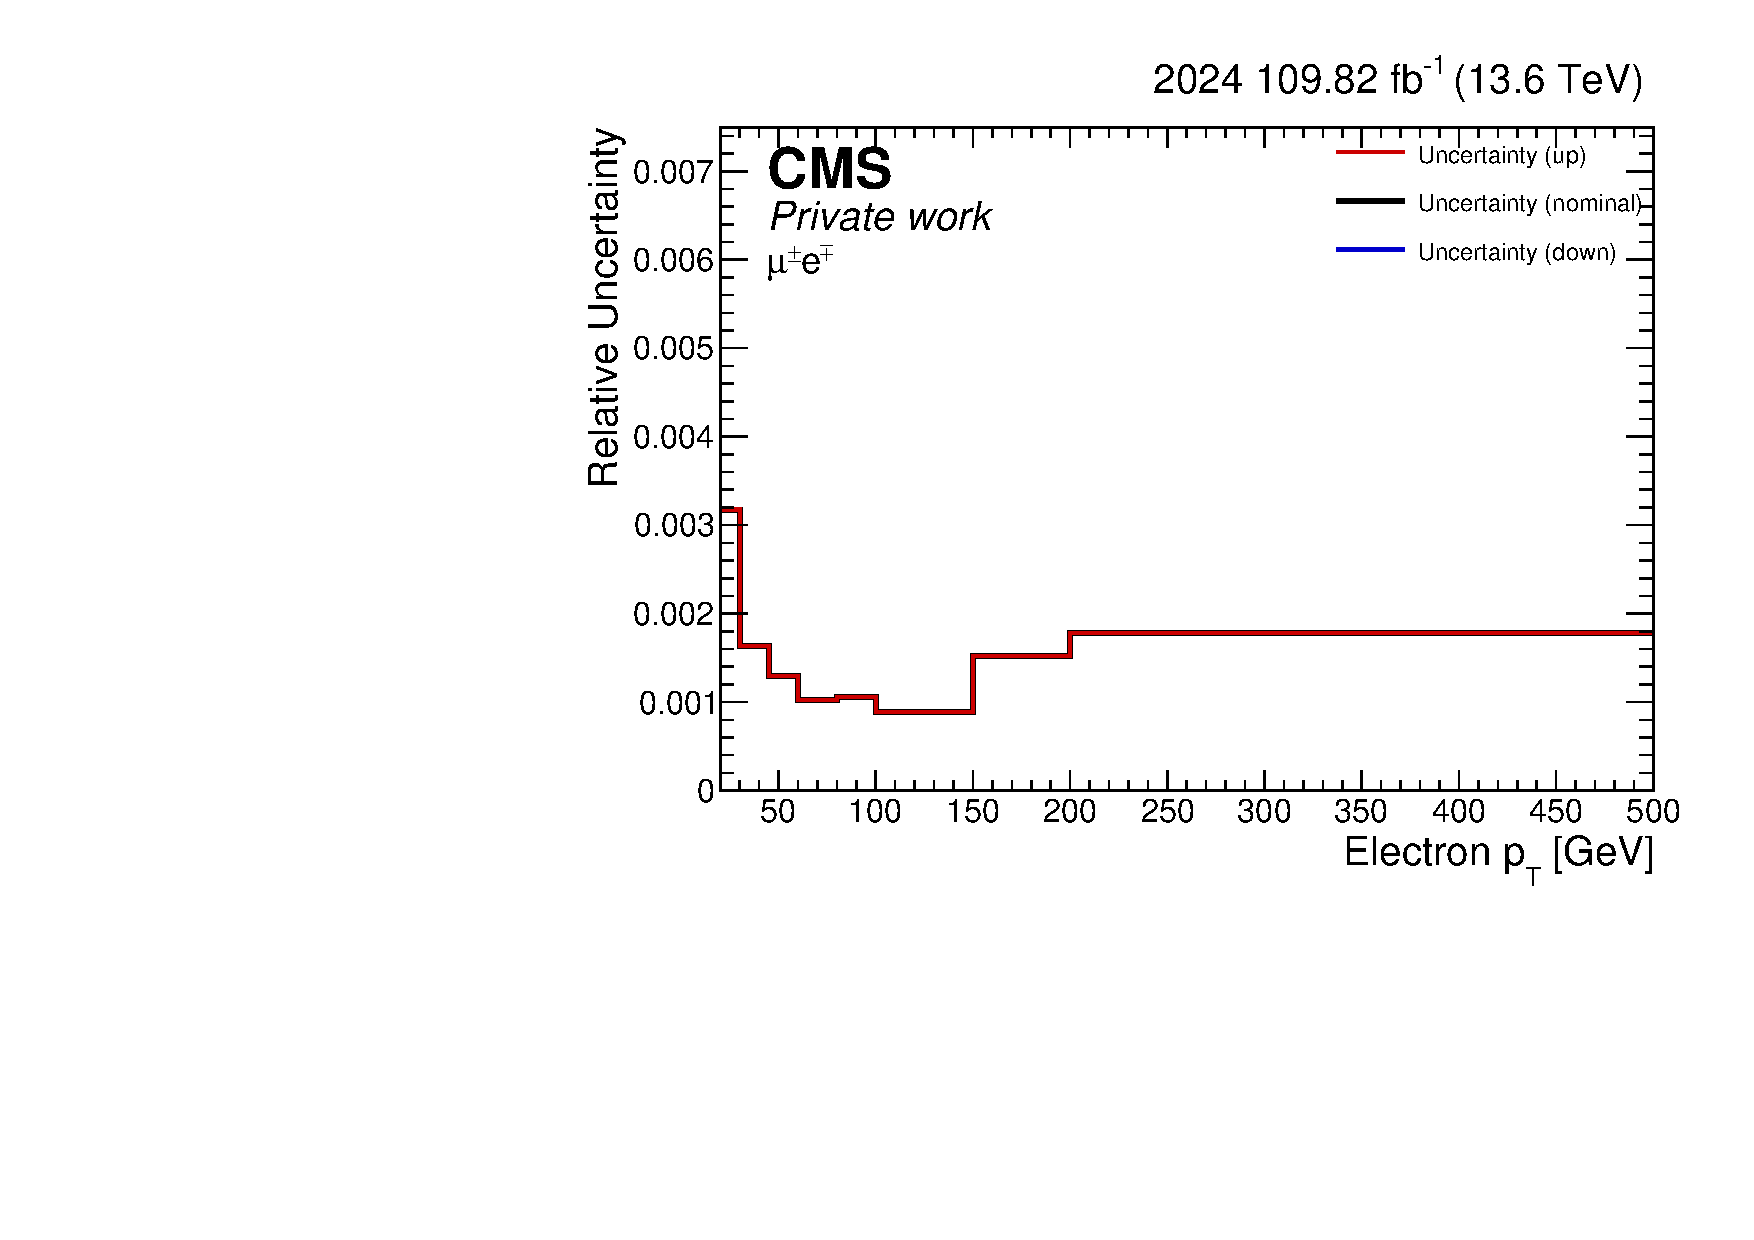
\includegraphics[width=0.48\linewidth]{figures/2024/MuEl/Statistical_Uncertainty/UncRatio_ElPt.pdf}
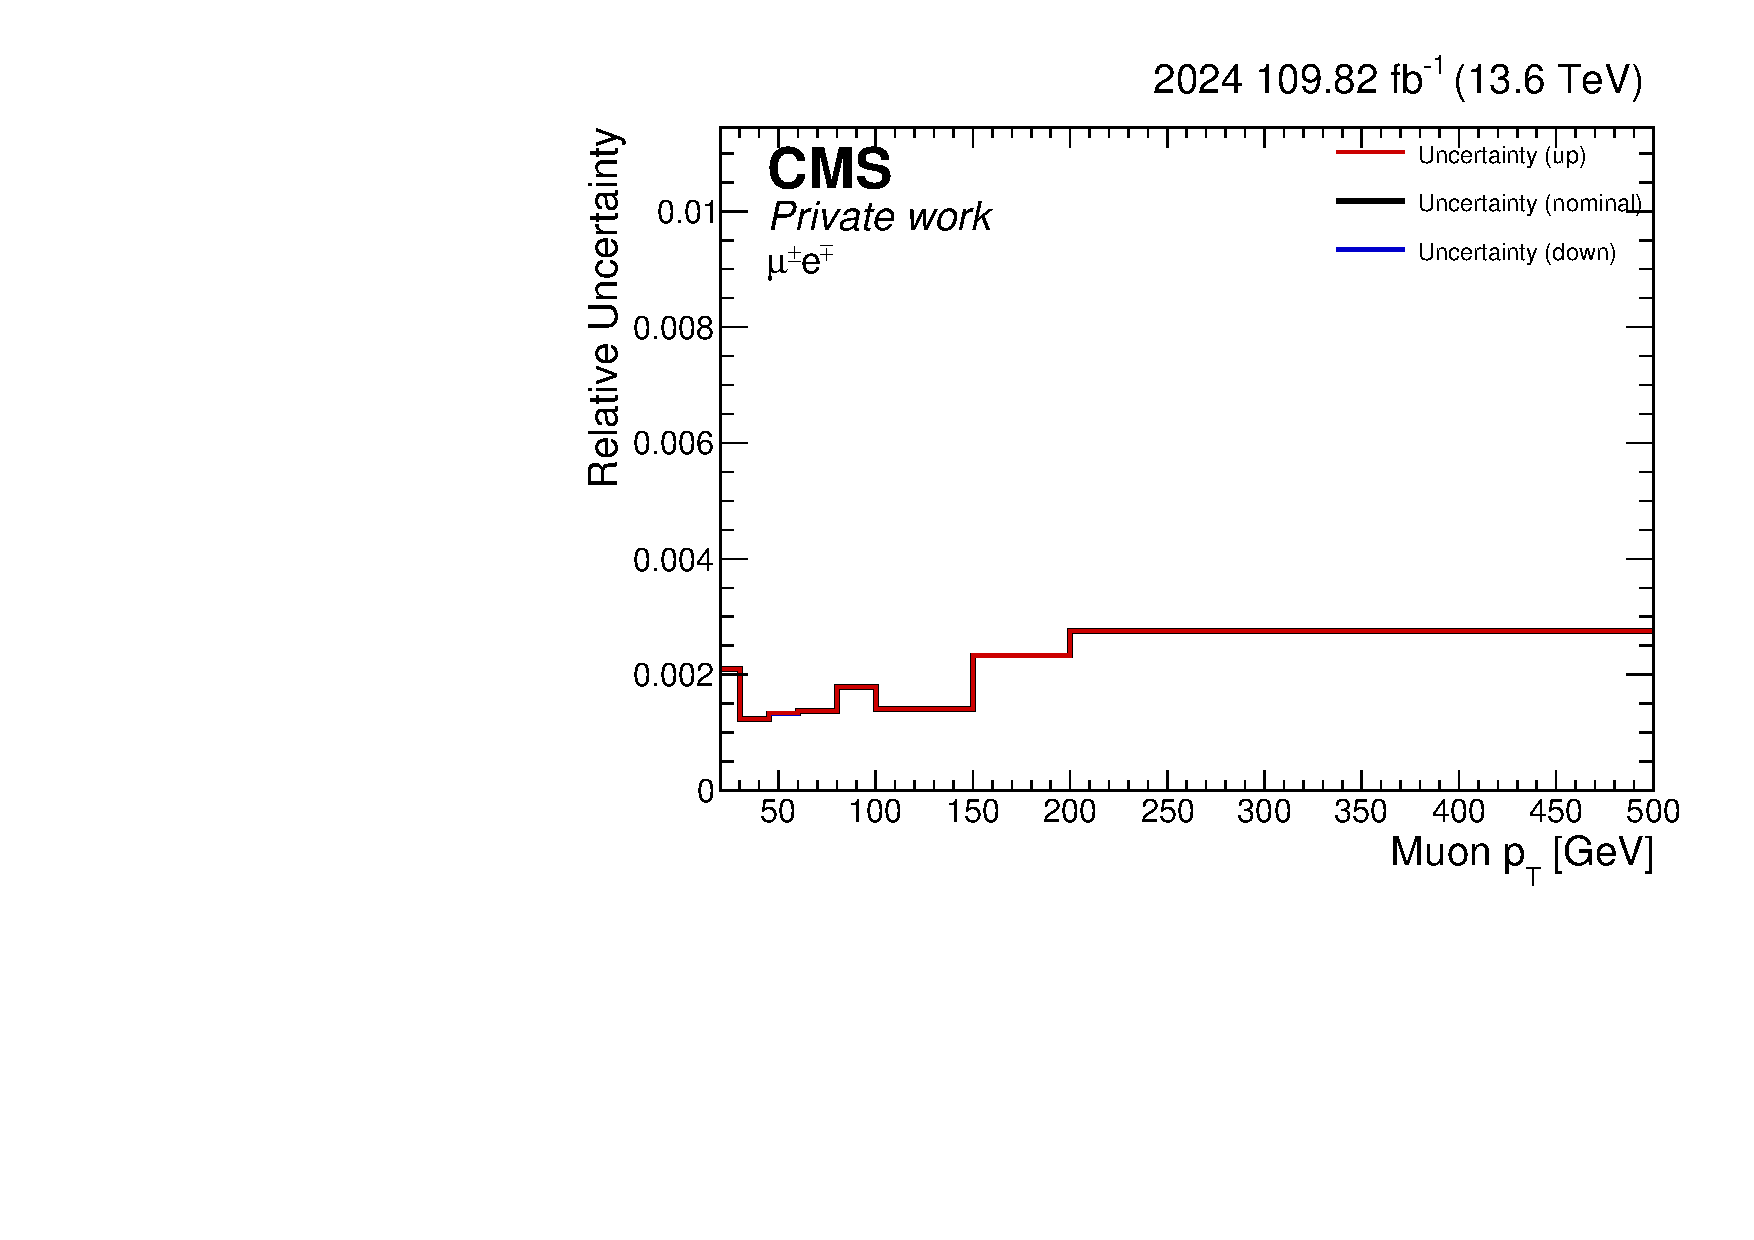
\includegraphics[width=0.48\linewidth]{figures/2024/MuEl/Statistical_Uncertainty/UncRatio_MuPt.pdf}
\caption{Relative statistical uncertainty diagnostics, retaining the nominal, upward, and downward curves of the supplied production in the $e\mu$ channel. Left and right: electron and muon $p_{\mathrm{T}}$.}\label{fig:extra-MuEl-Statistical-Uncertainty-ElPt}\end{figure}
\begin{figure}[p]\centering
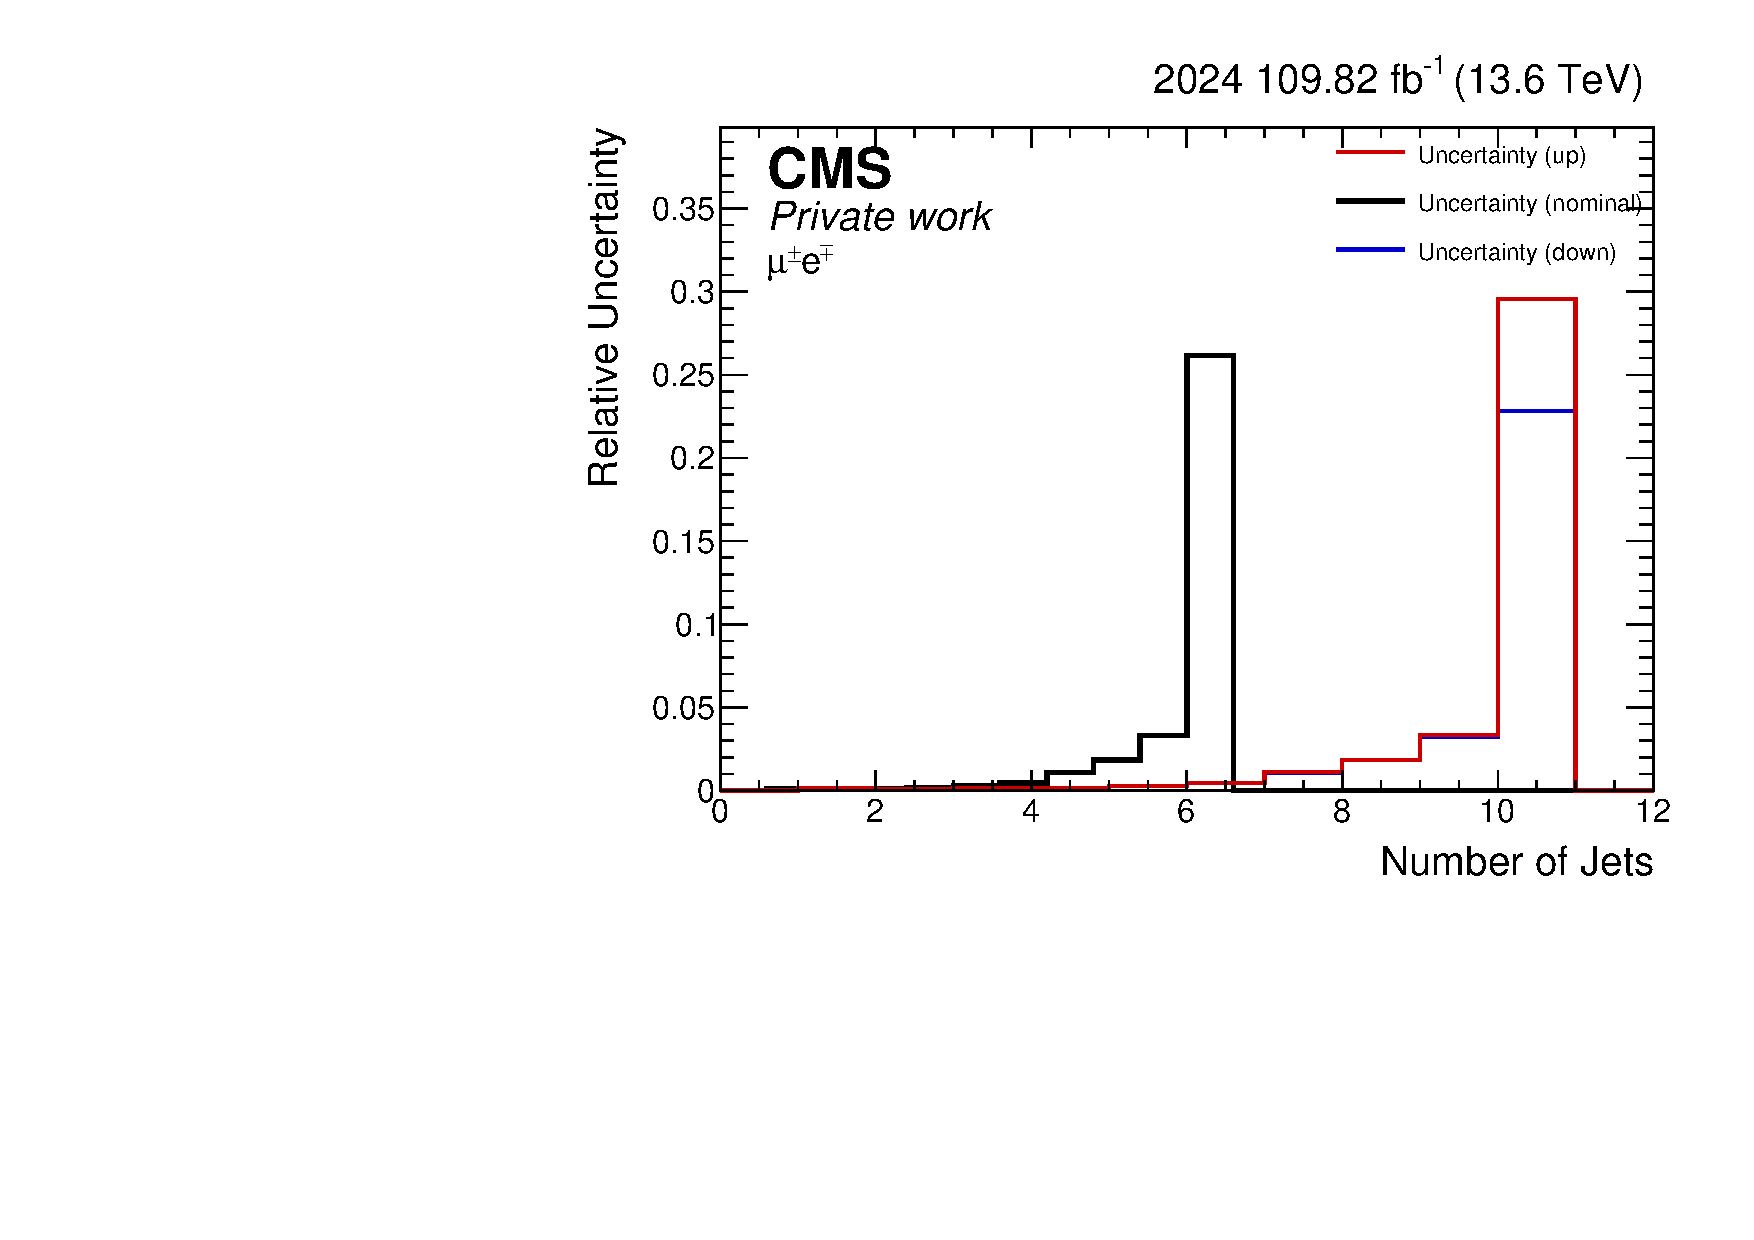
\includegraphics[width=0.48\linewidth]{figures/2024/MuEl/Statistical_Uncertainty/UncRatio_Num_Jets.pdf}
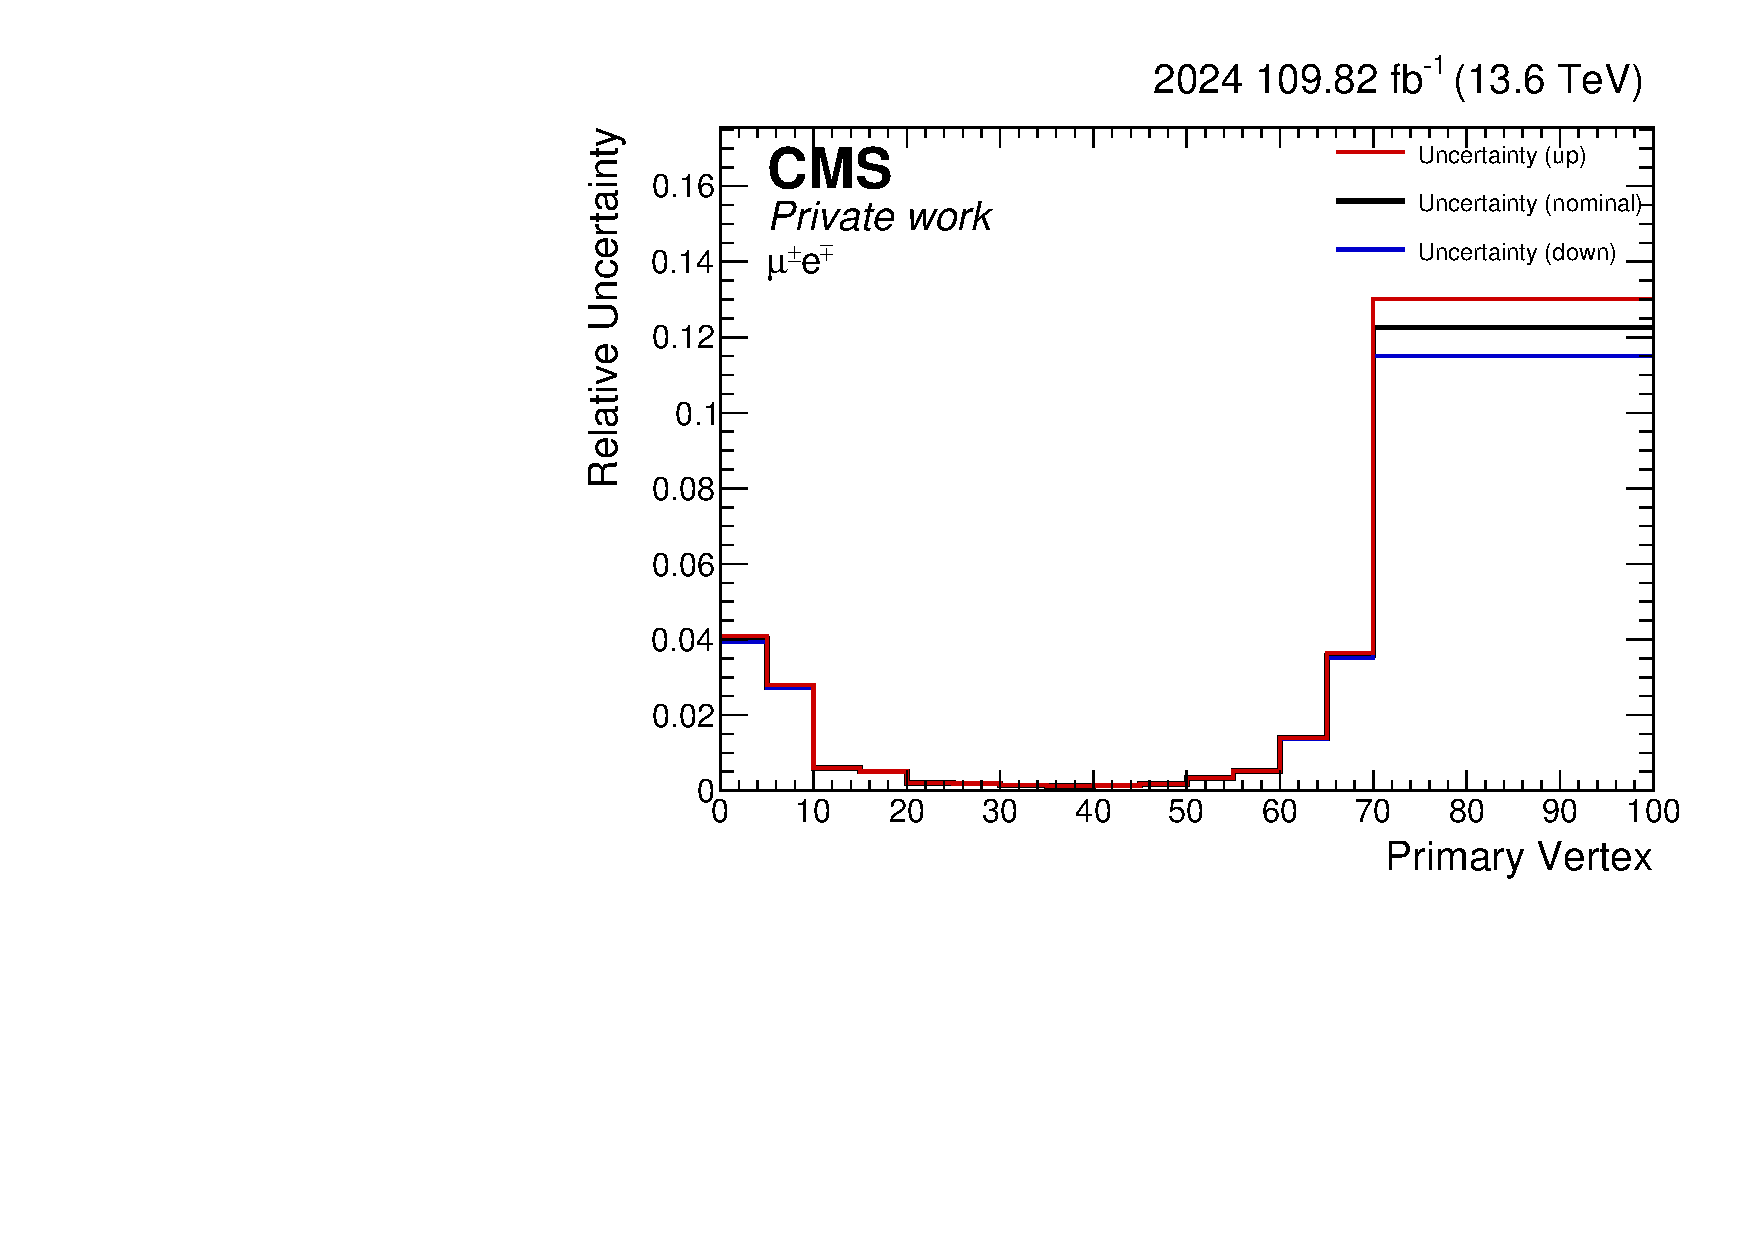
\includegraphics[width=0.48\linewidth]{figures/2024/MuEl/Statistical_Uncertainty/UncRatio_Num_PV.pdf}
\caption{Relative statistical uncertainty diagnostics, retaining the nominal, upward, and downward curves of the supplied production in the $e\mu$ channel. Left and right: jet and primary-vertex multiplicities.}\label{fig:extra-MuEl-Statistical-Uncertainty-Num_Jets}\end{figure}
\begin{figure}[p]\centering
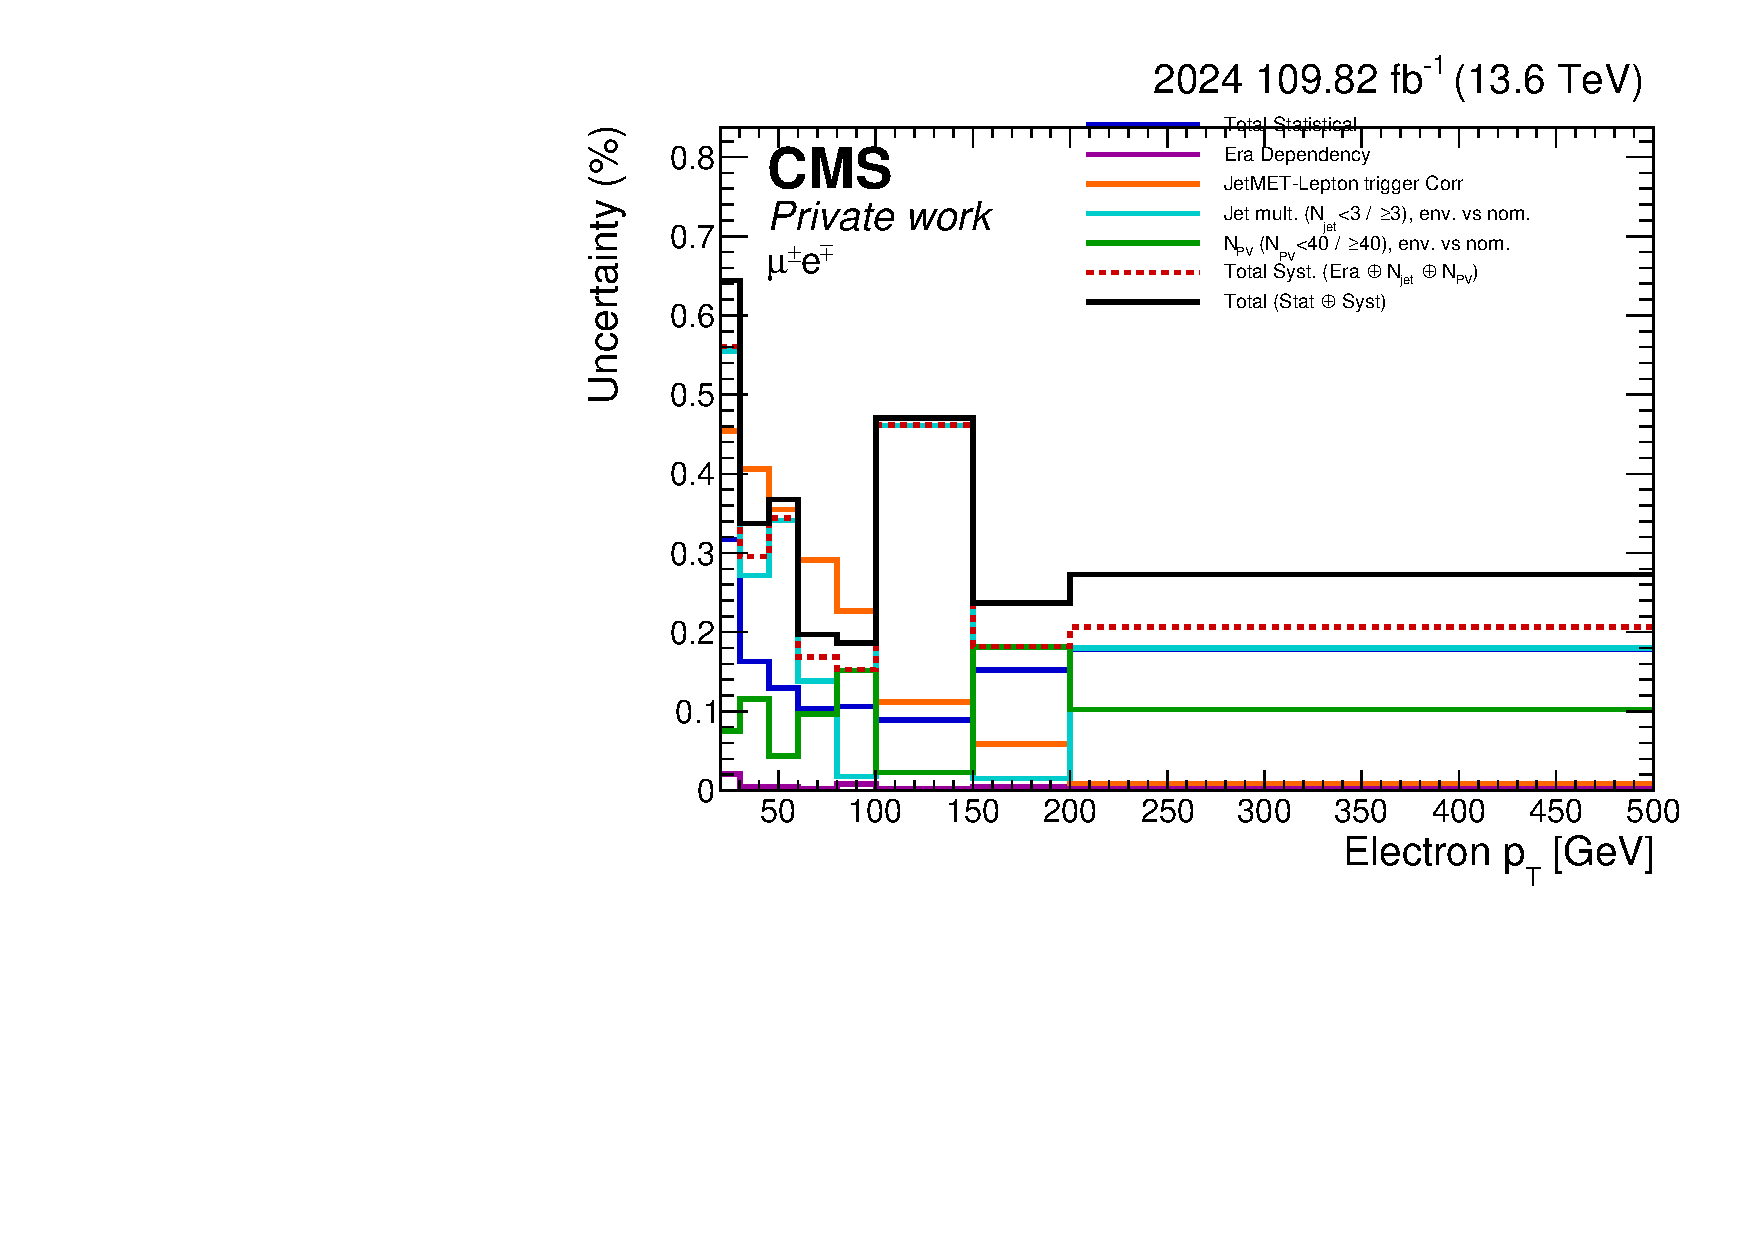
\includegraphics[width=0.48\linewidth]{figures/2024/MuEl/Uncertainty_Breakdown/Breakdown_ElPt.pdf}
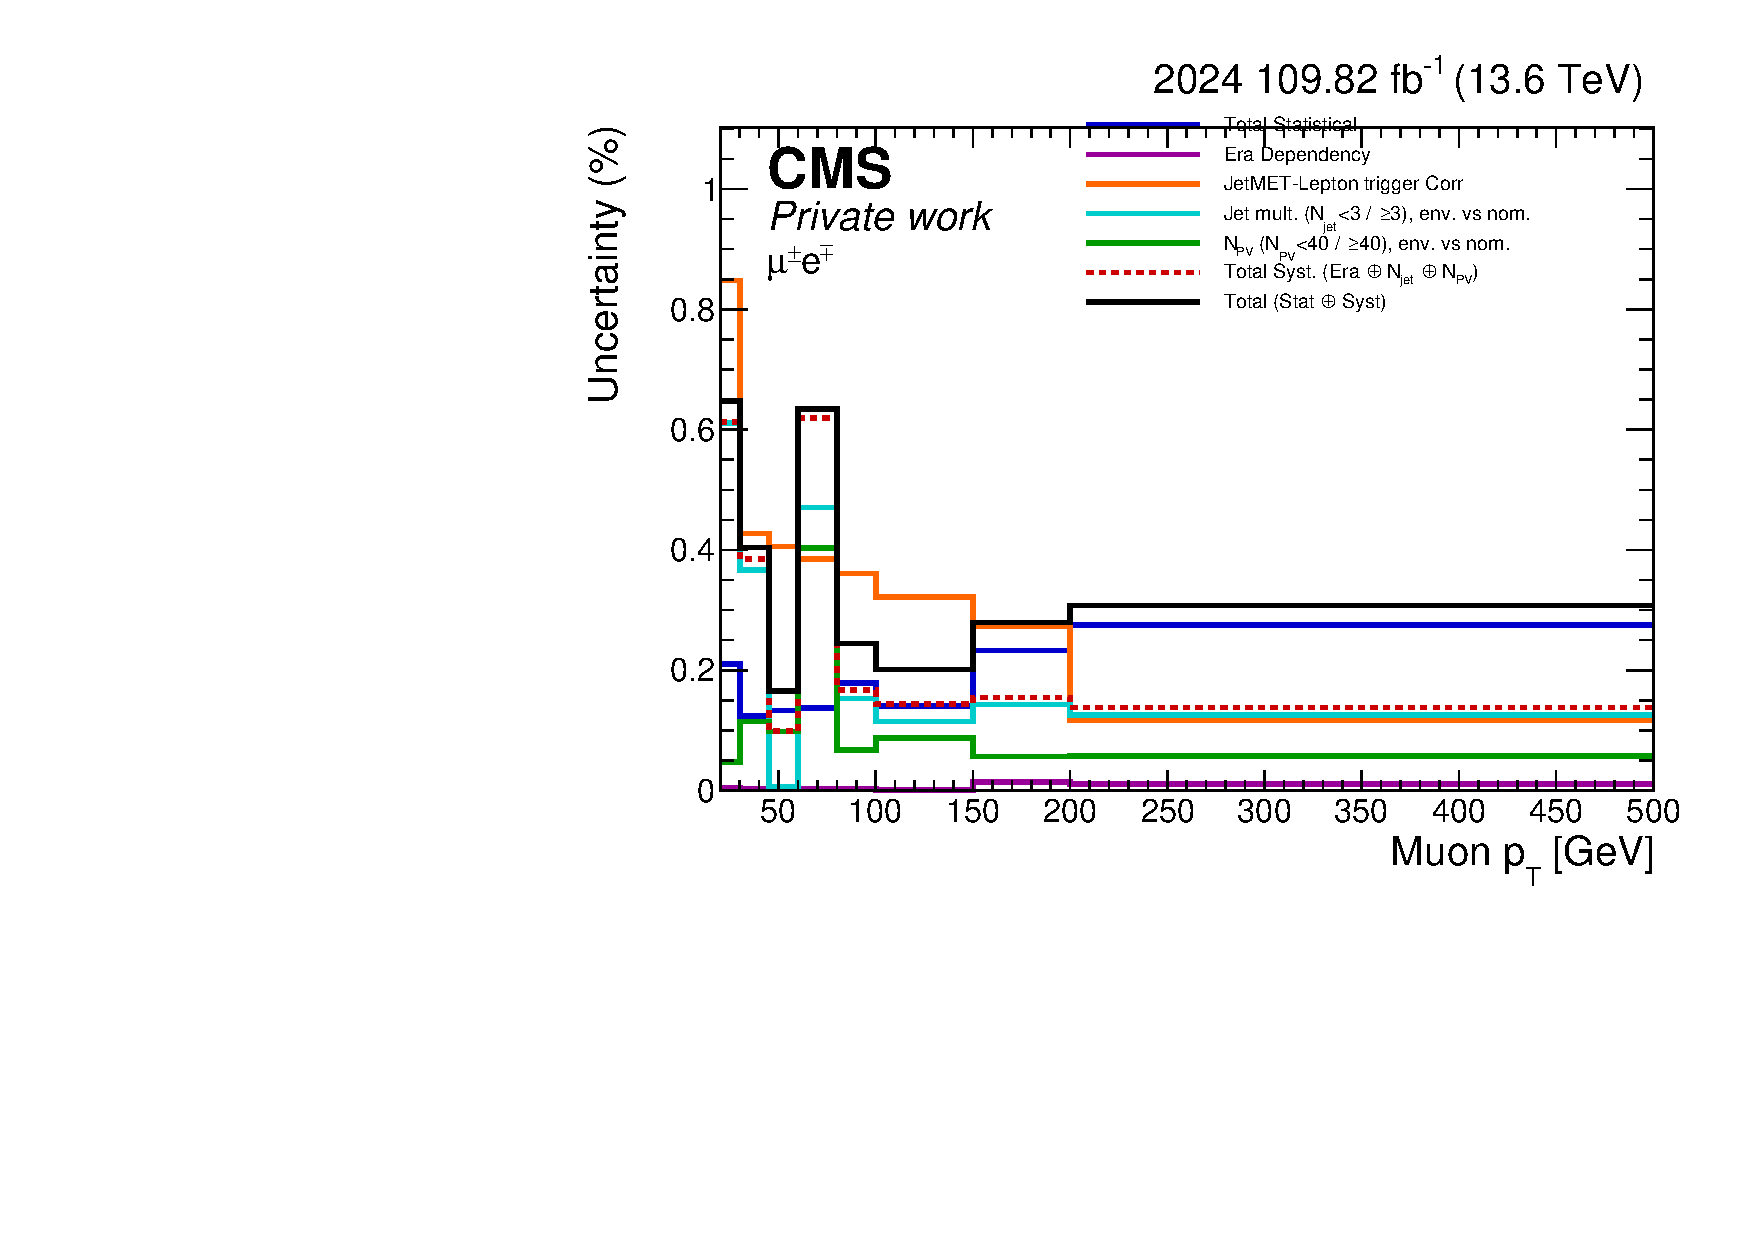
\includegraphics[width=0.48\linewidth]{figures/2024/MuEl/Uncertainty_Breakdown/Breakdown_MuPt.pdf}
\caption{Absolute uncertainty component breakdown in the $e\mu$ channel. Left and right: electron and muon $p_{\mathrm{T}}$.}\label{fig:extra-MuEl-Uncertainty-Breakdown-ElPt}\end{figure}
\begin{figure}[p]\centering
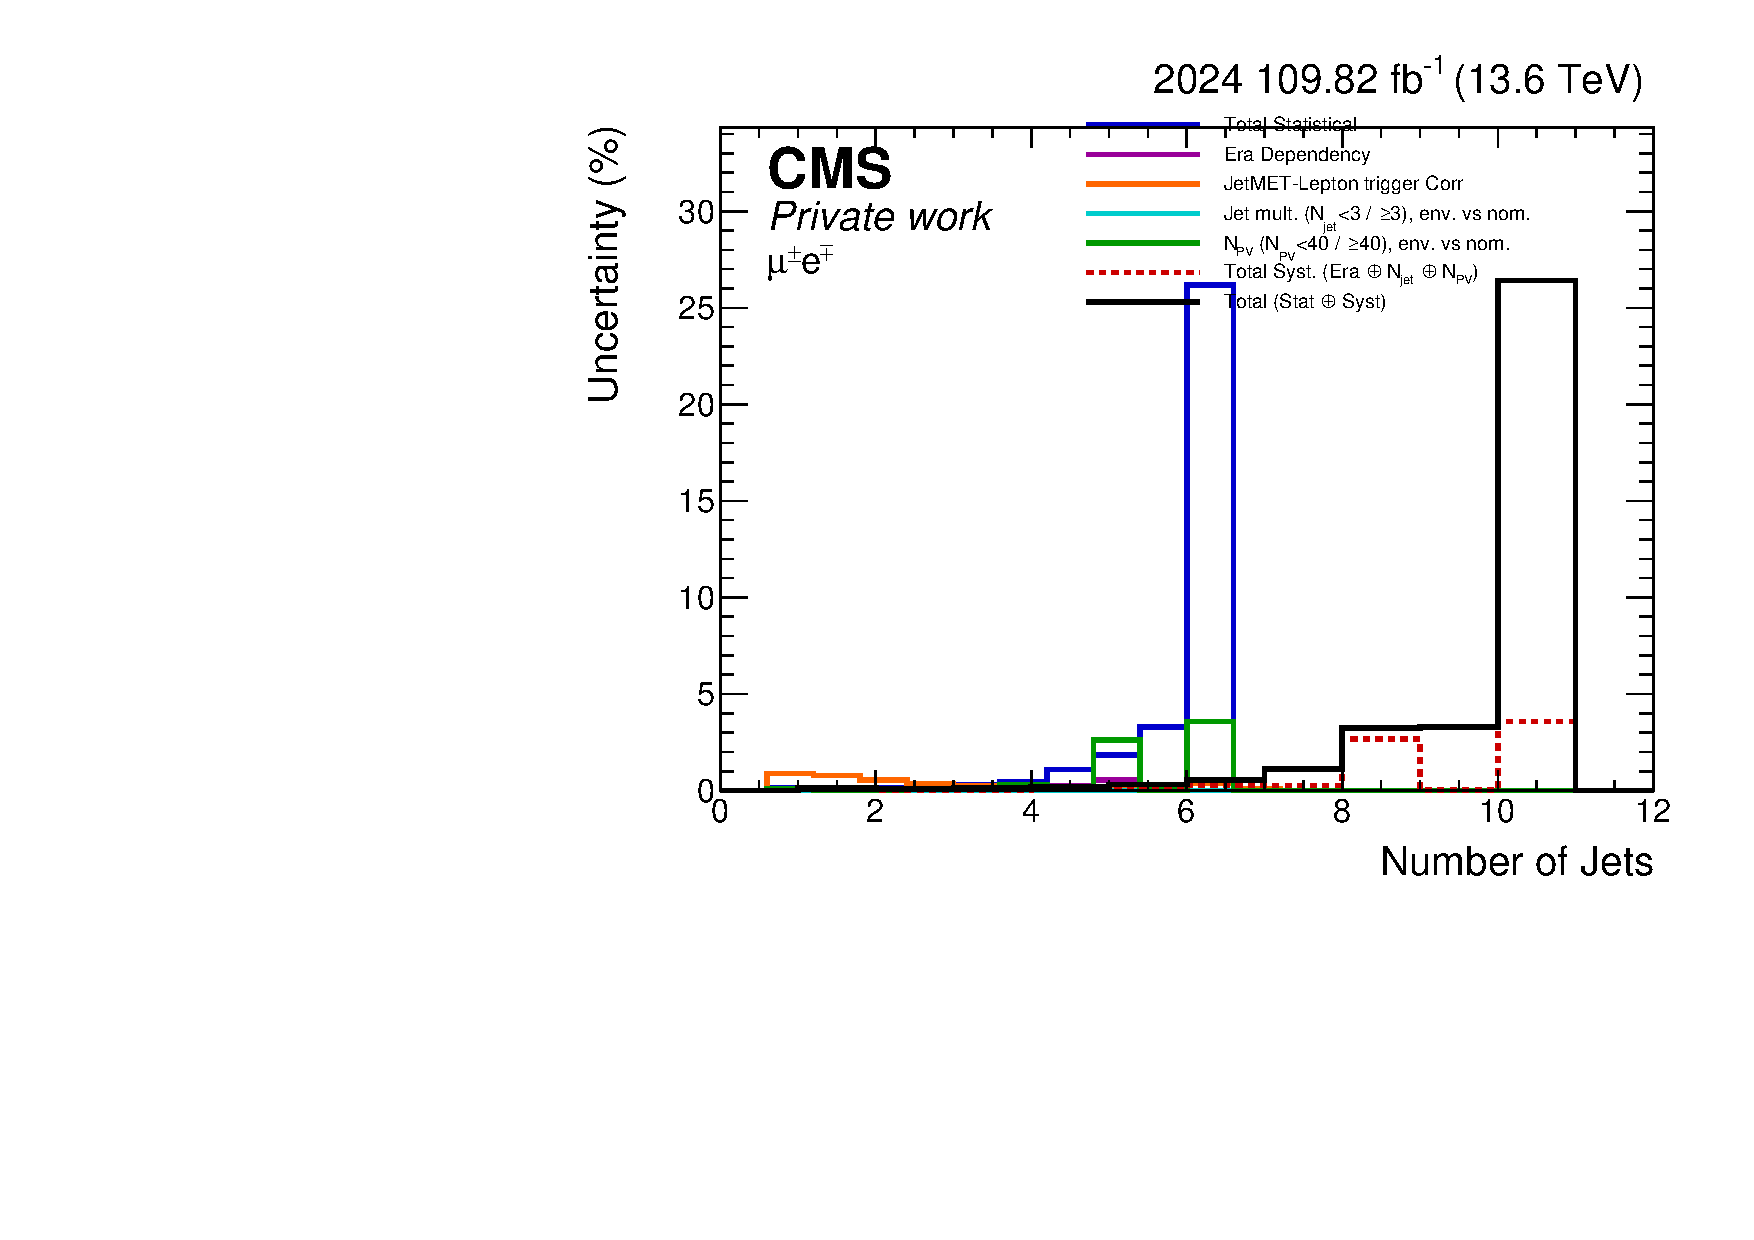
\includegraphics[width=0.48\linewidth]{figures/2024/MuEl/Uncertainty_Breakdown/Breakdown_Num_Jets.pdf}
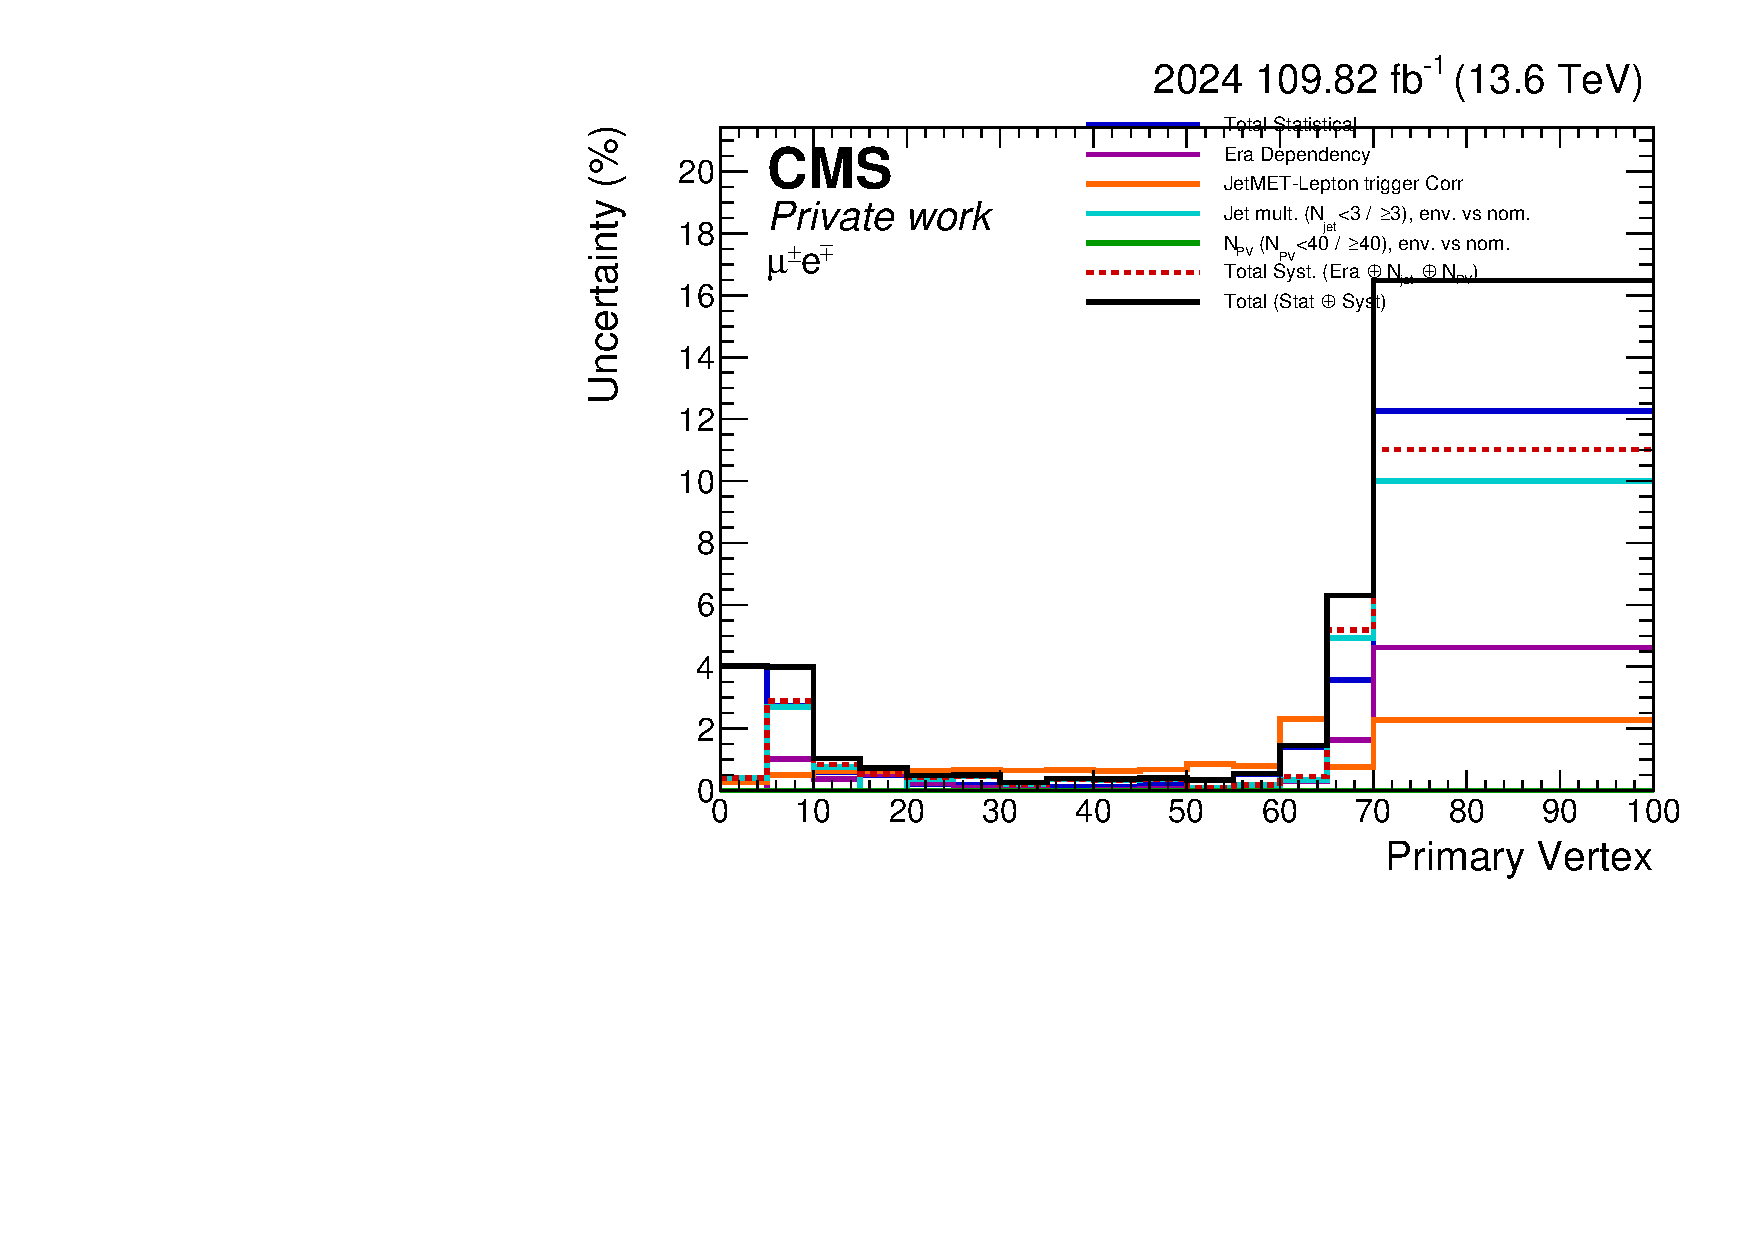
\includegraphics[width=0.48\linewidth]{figures/2024/MuEl/Uncertainty_Breakdown/Breakdown_Num_PV.pdf}
\caption{Absolute uncertainty component breakdown in the $e\mu$ channel. Left and right: jet and primary-vertex multiplicities.}\label{fig:extra-MuEl-Uncertainty-Breakdown-Num_Jets}\end{figure}
\begin{figure}[p]\centering
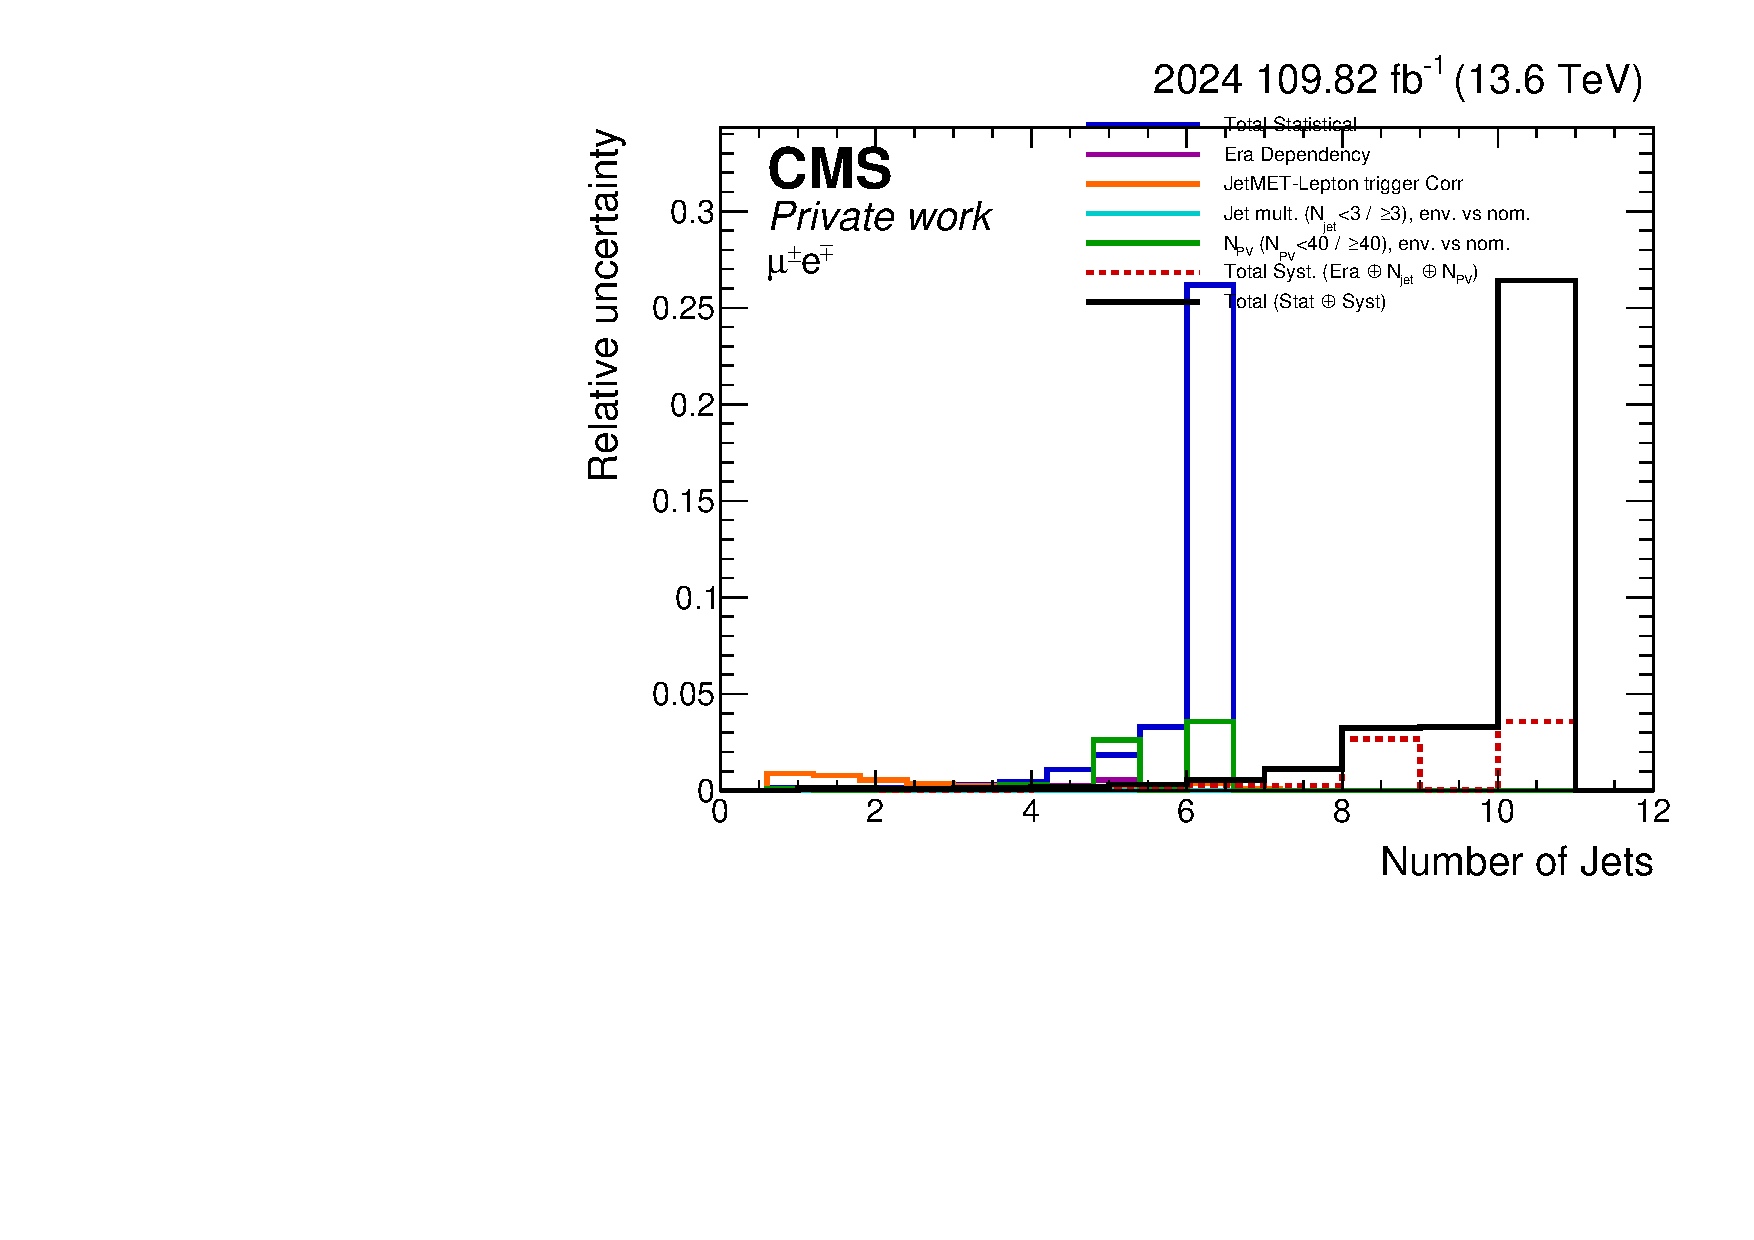
\includegraphics[width=0.48\linewidth]{figures/2024/MuEl/Relative_Uncertainty_Breakdown/Breakdown_Num_Jets.pdf}
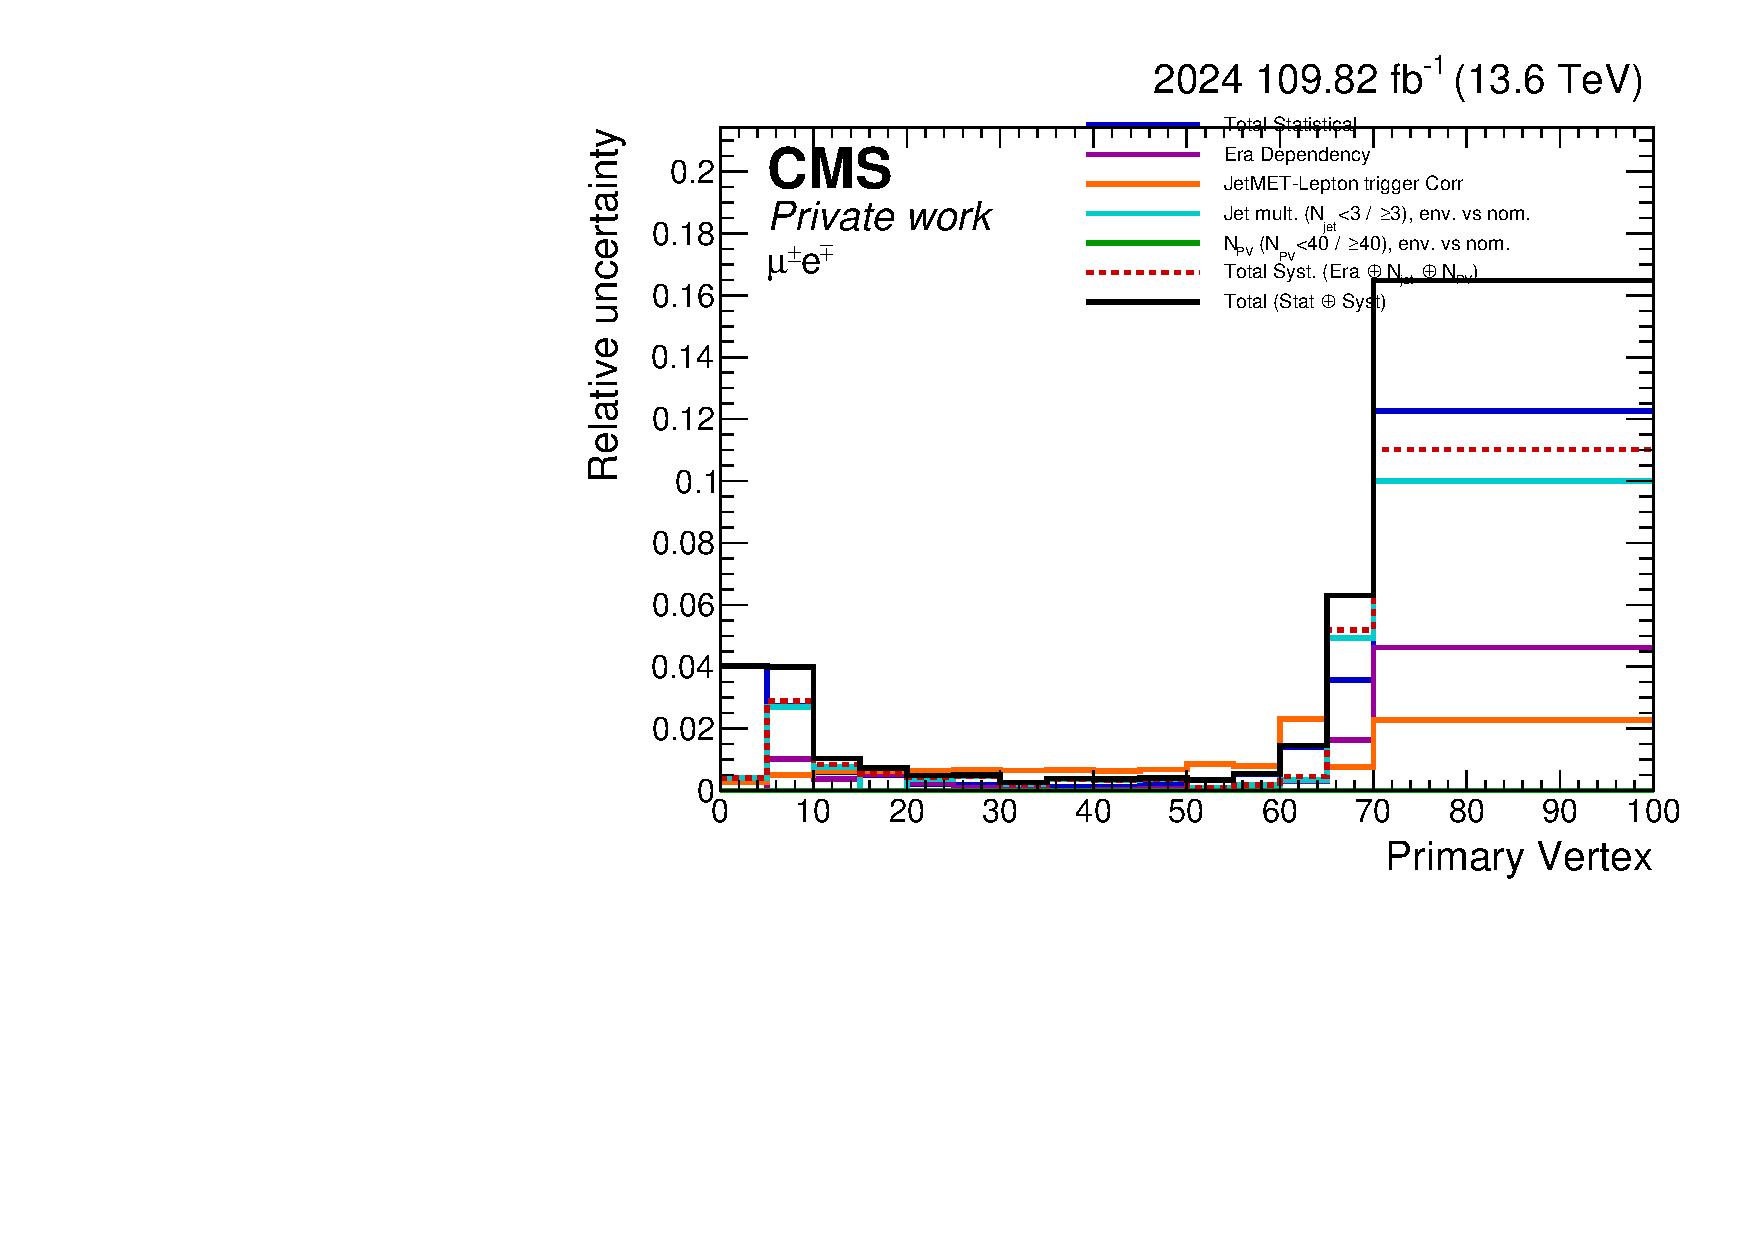
\includegraphics[width=0.48\linewidth]{figures/2024/MuEl/Relative_Uncertainty_Breakdown/Breakdown_Num_PV.pdf}
\caption{Relative uncertainty component breakdown versus event activity in the $e\mu$ channel. Left and right: jet and primary-vertex multiplicities.}\label{fig:extra-MuEl-Relative-Uncertainty-Breakdown-Num_Jets}\end{figure}
\begin{figure}[p]\centering
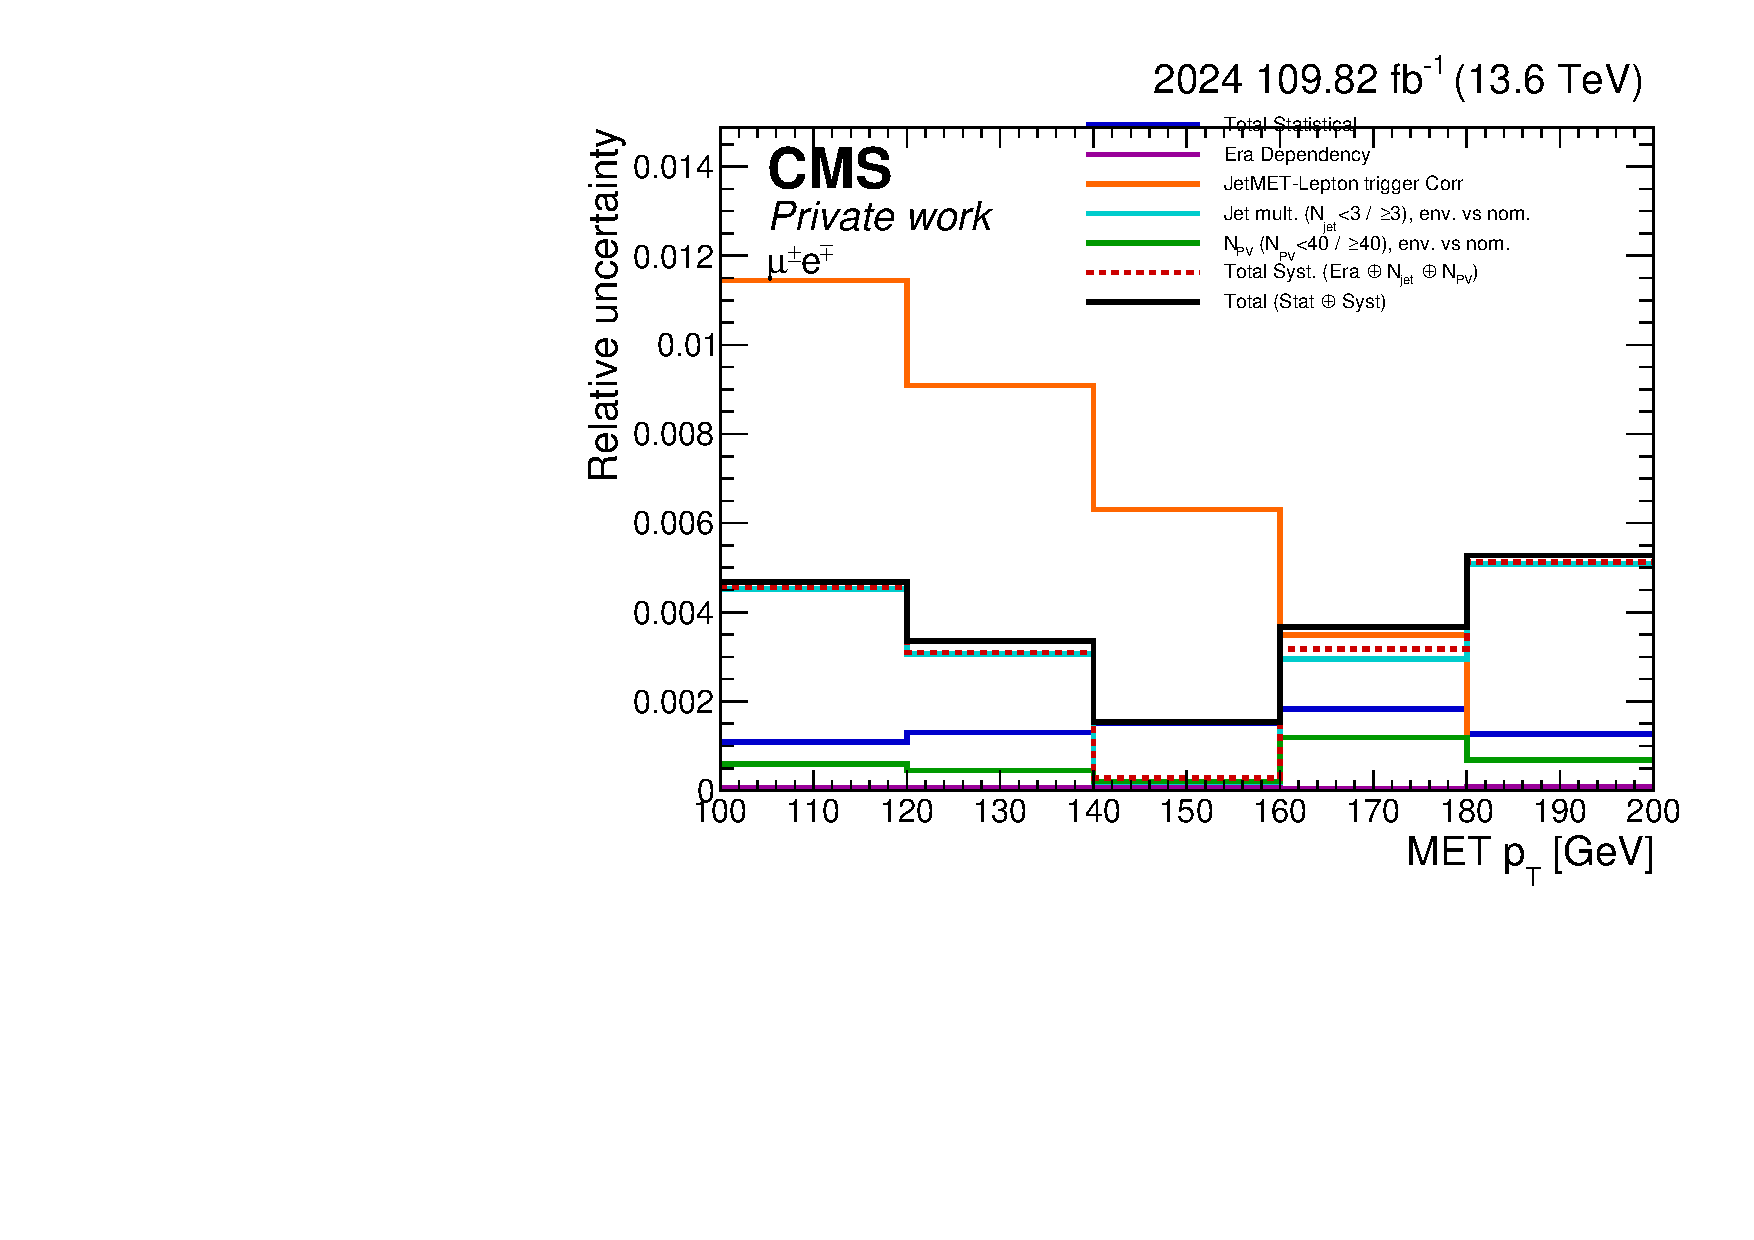
\includegraphics[width=0.48\linewidth]{figures/2024/MuEl/Relative_Uncertainty_Breakdown/Breakdown_METpt.pdf}
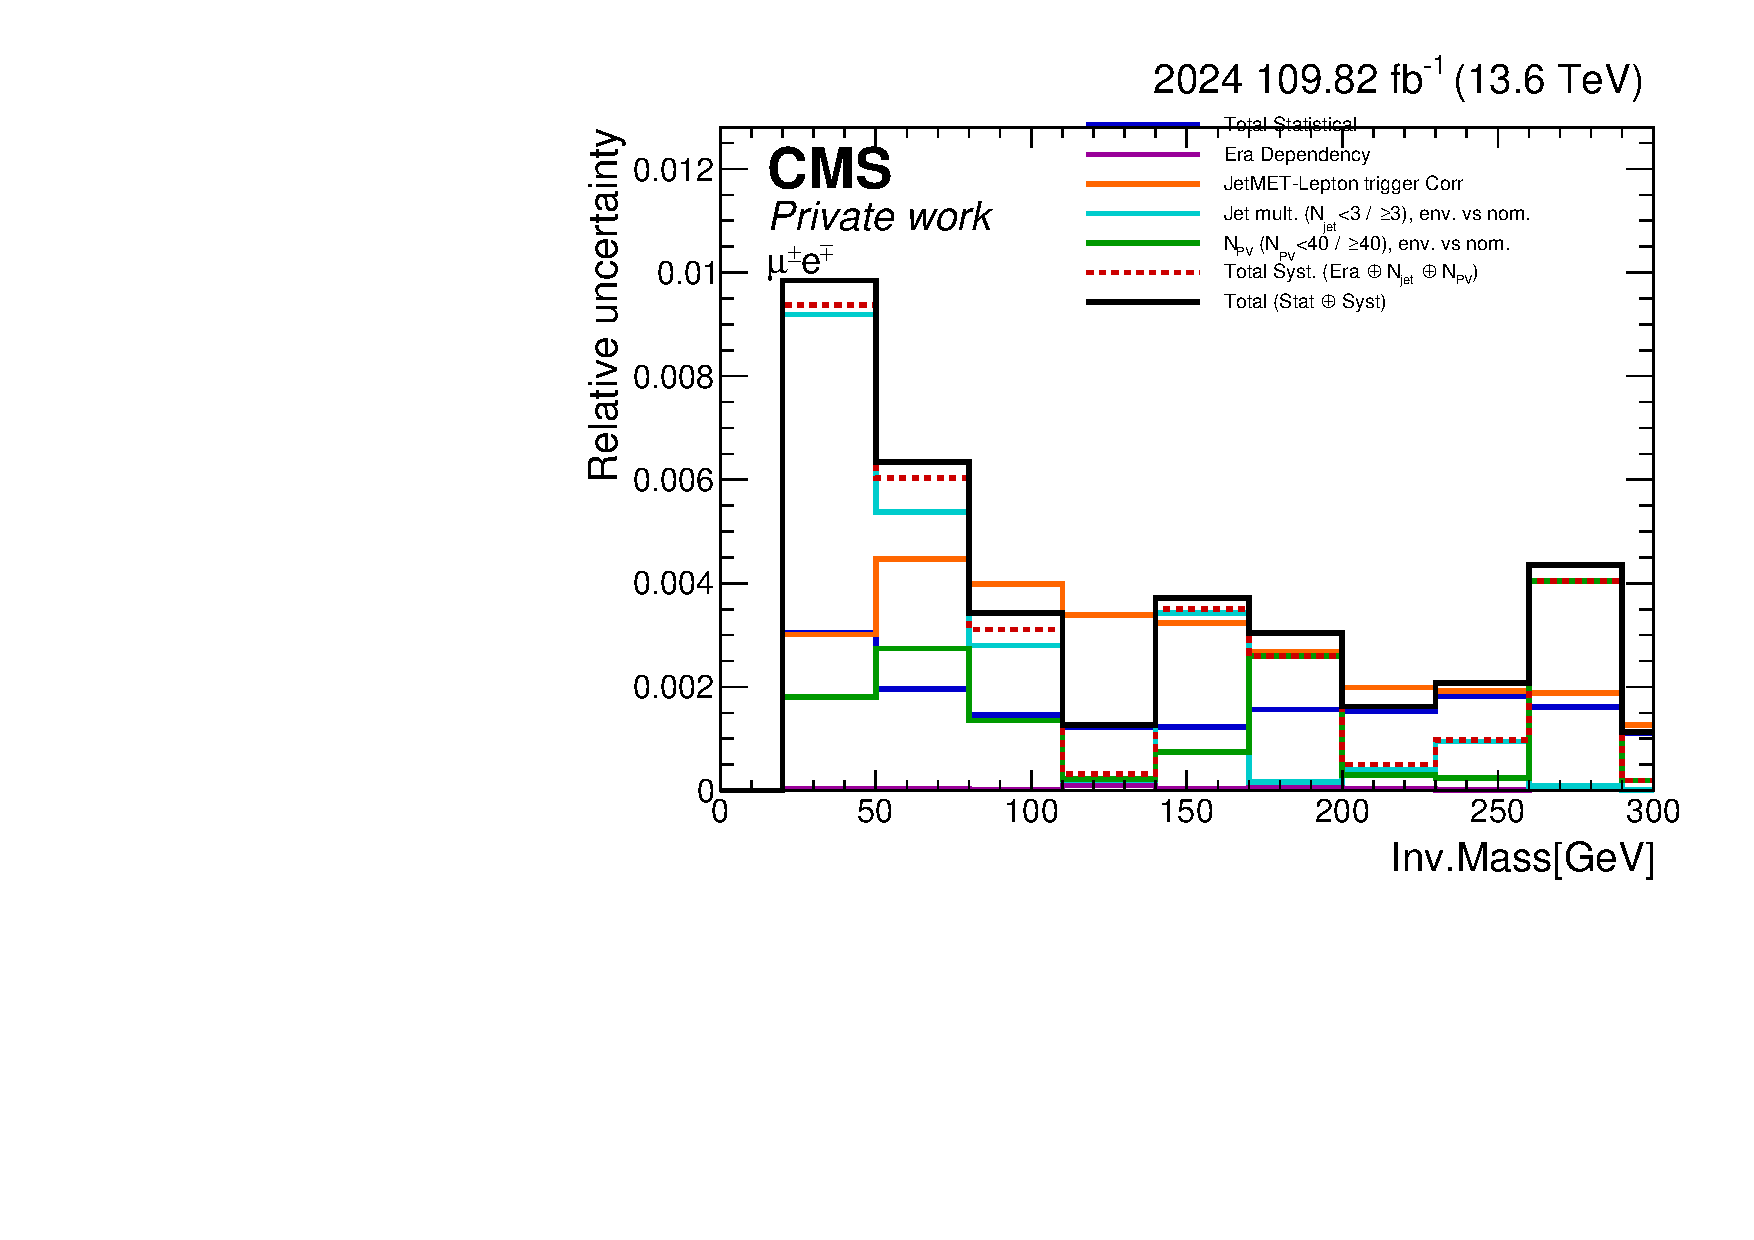
\includegraphics[width=0.48\linewidth]{figures/2024/MuEl/Relative_Uncertainty_Breakdown/Breakdown_DiLepMass.pdf}
\caption{Relative uncertainty component breakdown versus event kinematics in the $e\mu$ channel. Left and right: missing transverse momentum and dilepton invariant mass.}\label{fig:extra-MuEl-Relative-Uncertainty-Breakdown-METpt}\end{figure}
\begin{figure}[p]\centering
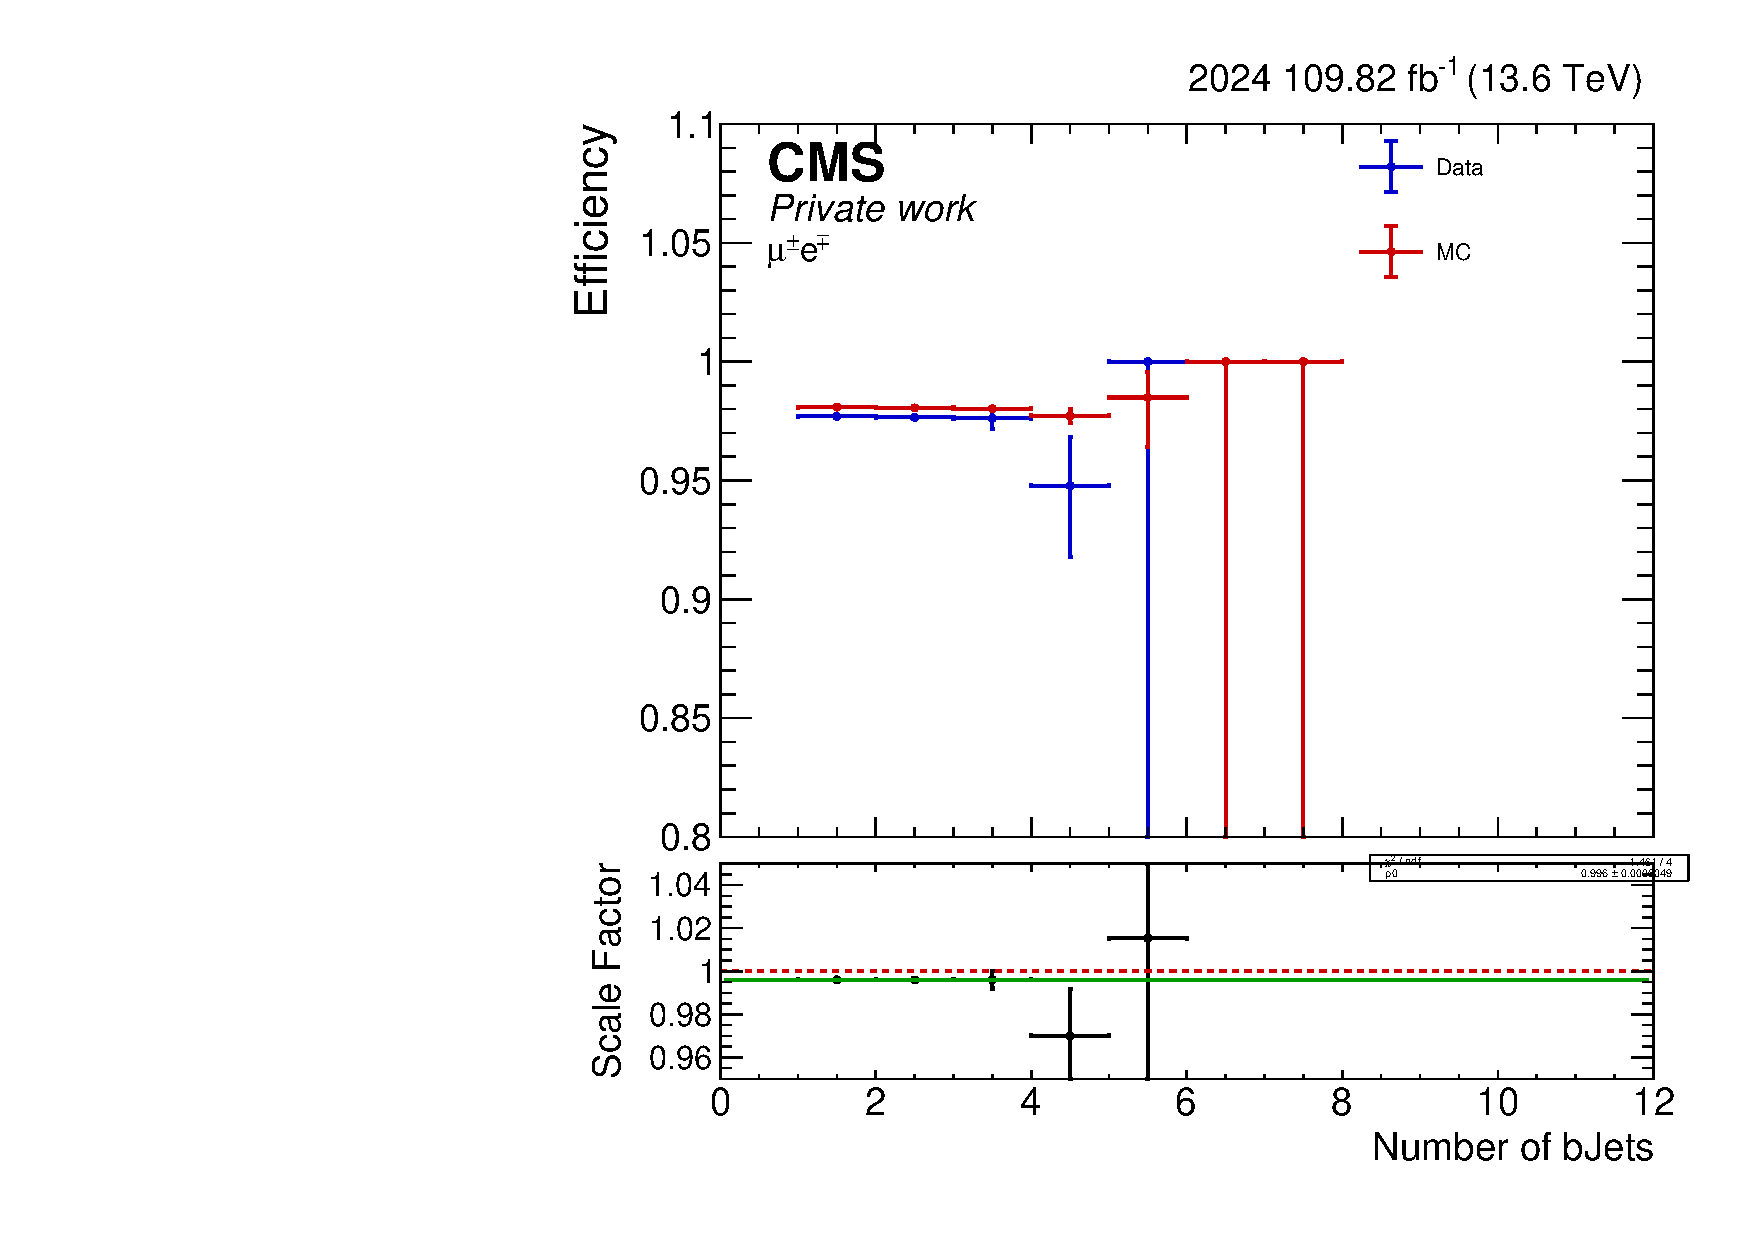
\includegraphics[width=0.48\linewidth]{figures/2024/MuEl/ScaleFactor/SF_Num_bJets.pdf}
\caption{Efficiency comparison and scale factor versus heavy-flavour activity in the $e\mu$ channel. $b$-tagged jet multiplicity.}\label{fig:extra-MuEl-ScaleFactor-Num_bJets}\end{figure}
\begin{figure}[p]\centering
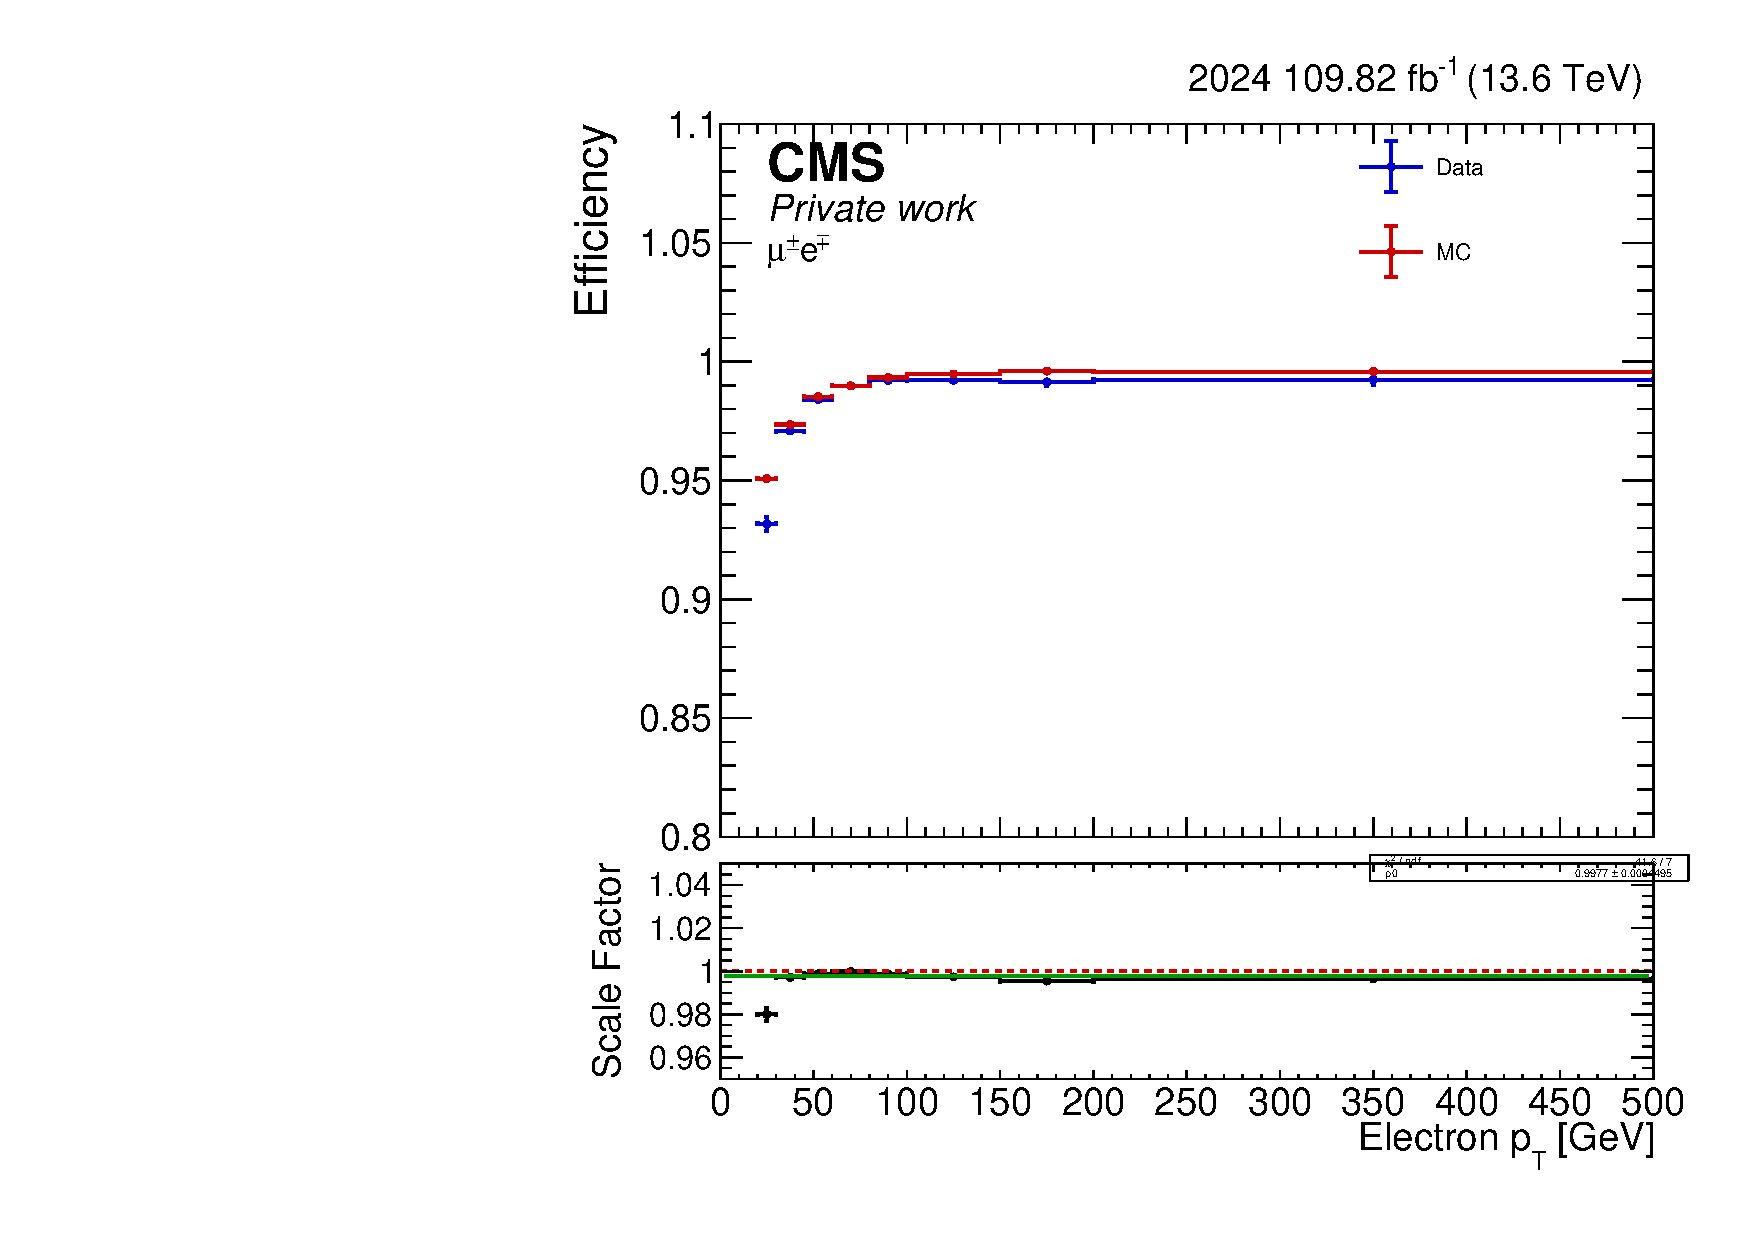
\includegraphics[width=0.48\linewidth]{figures/2024/MuEl/ScaleFactor/SF_ElPt.pdf}
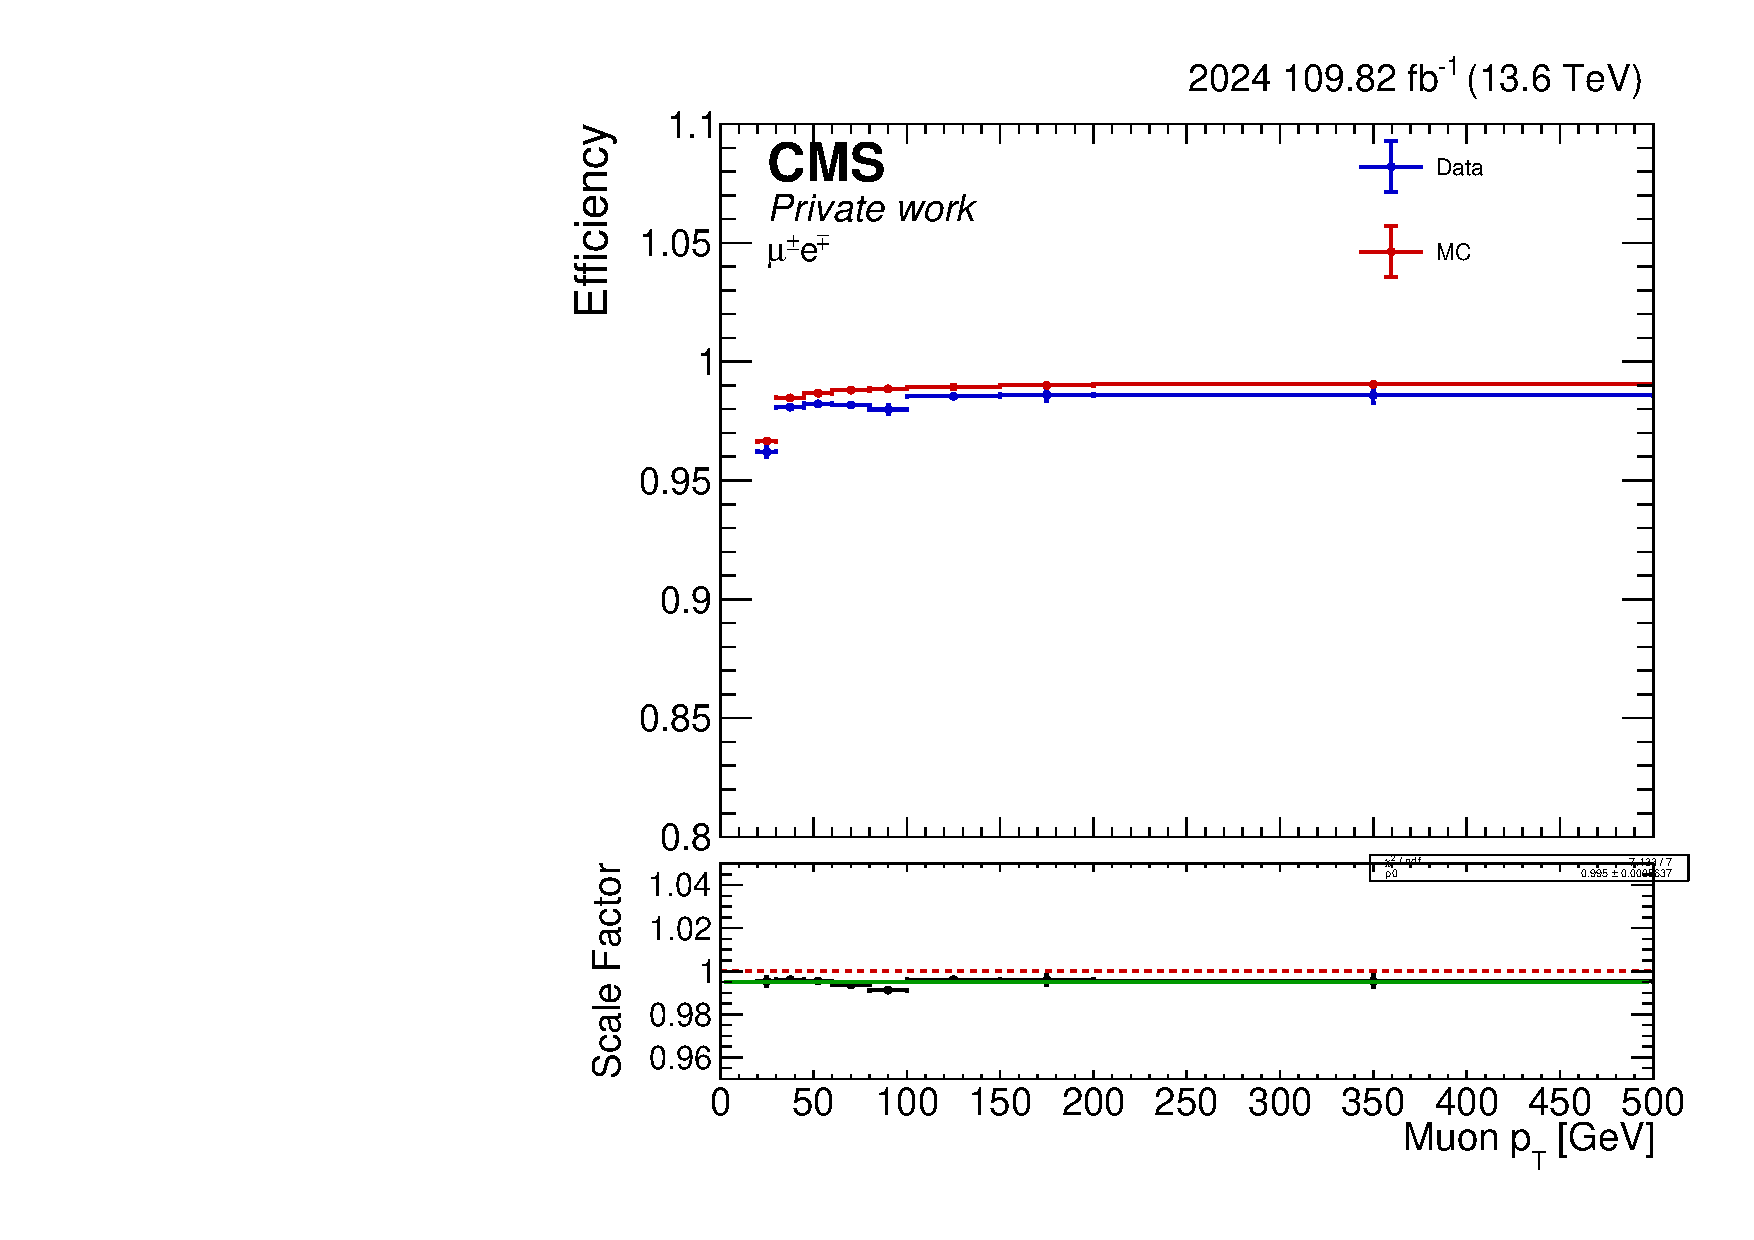
\includegraphics[width=0.48\linewidth]{figures/2024/MuEl/ScaleFactor/SF_MuPt.pdf}
\caption{Efficiency comparison and scale factor in the flavour-specific momentum variables used by the two-dimensional correction in the $e\mu$ channel. Left and right: electron and muon $p_{\mathrm{T}}$.}\label{fig:extra-MuEl-ScaleFactor-ElPt}\end{figure}
\clearpage\subsection{$\mu\mu$ channel}
\begin{figure}[p]\centering
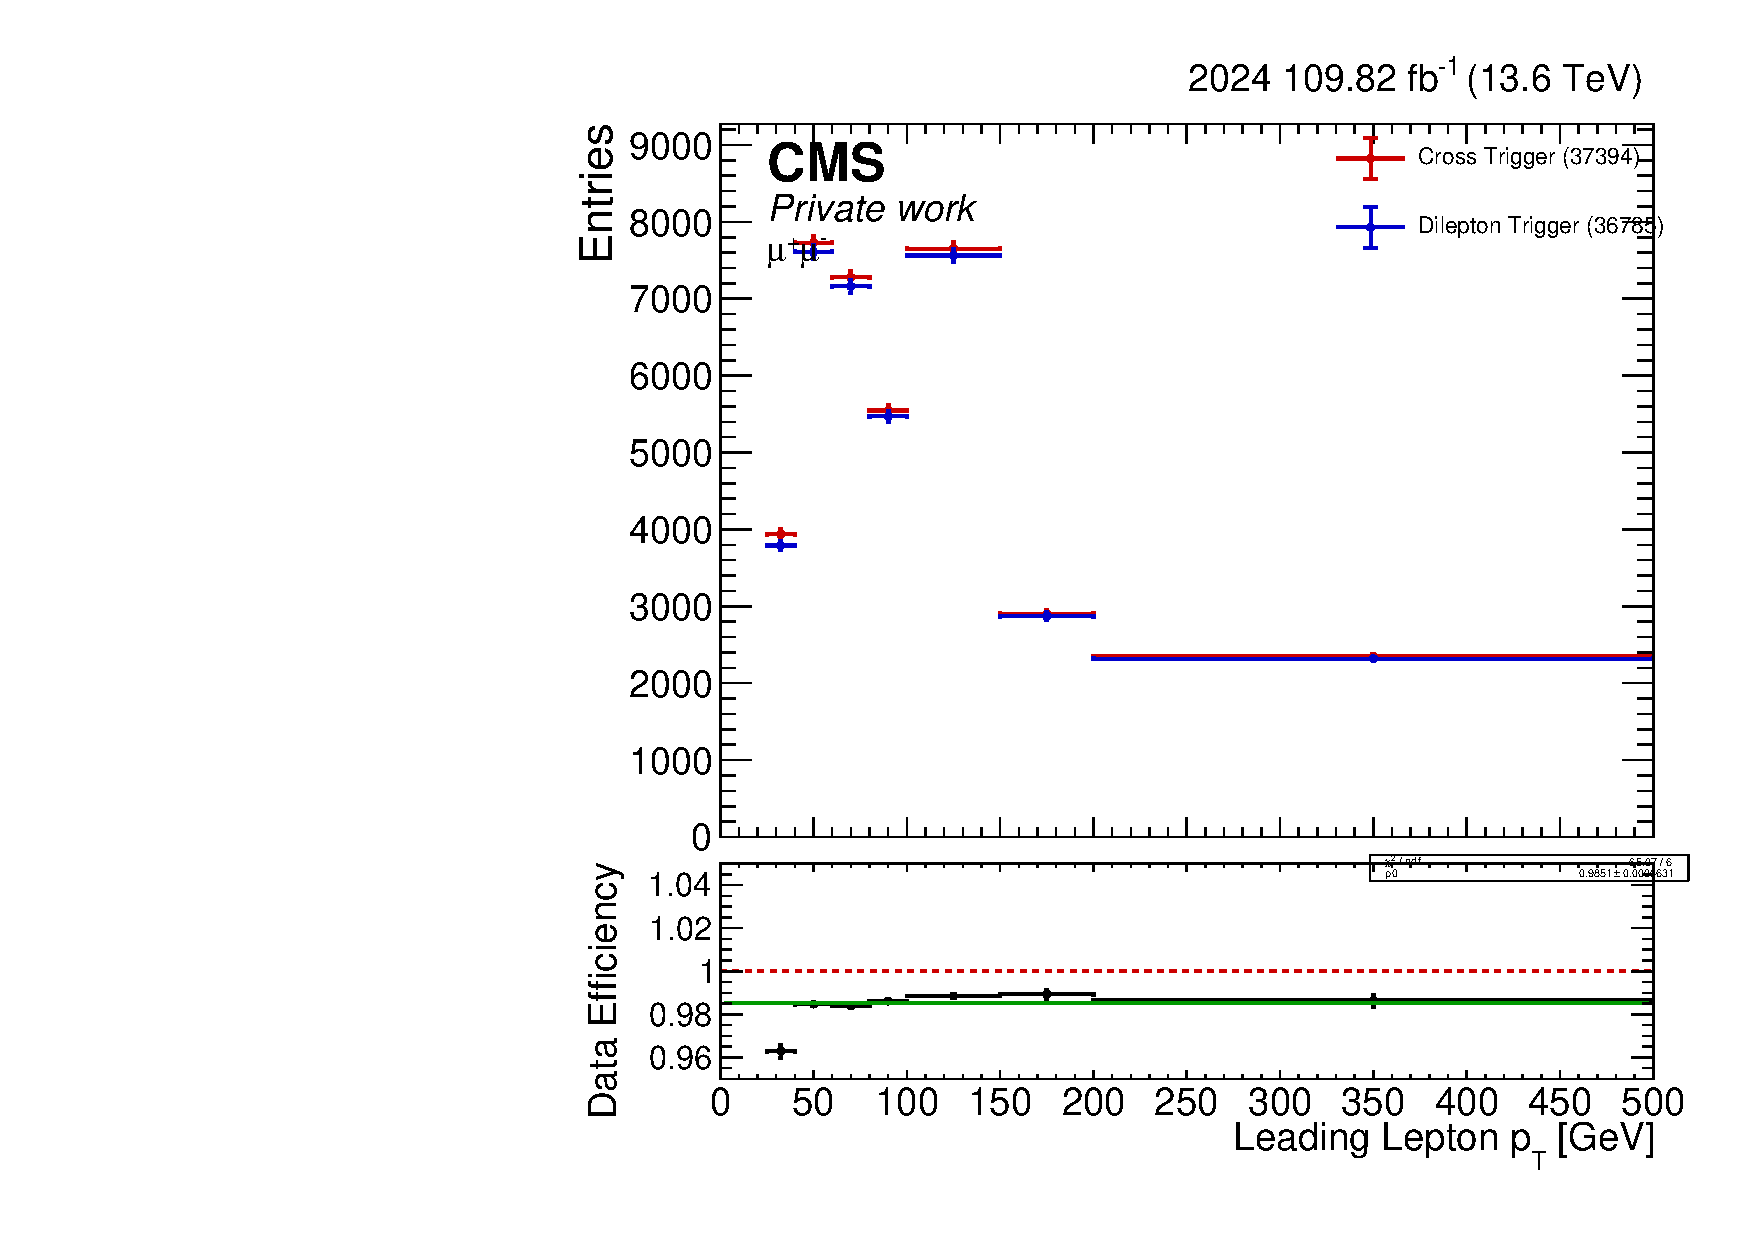
\includegraphics[width=0.48\linewidth]{figures/2024/MuMu/TrigEffData/TrigEff_Lep1pt.pdf}
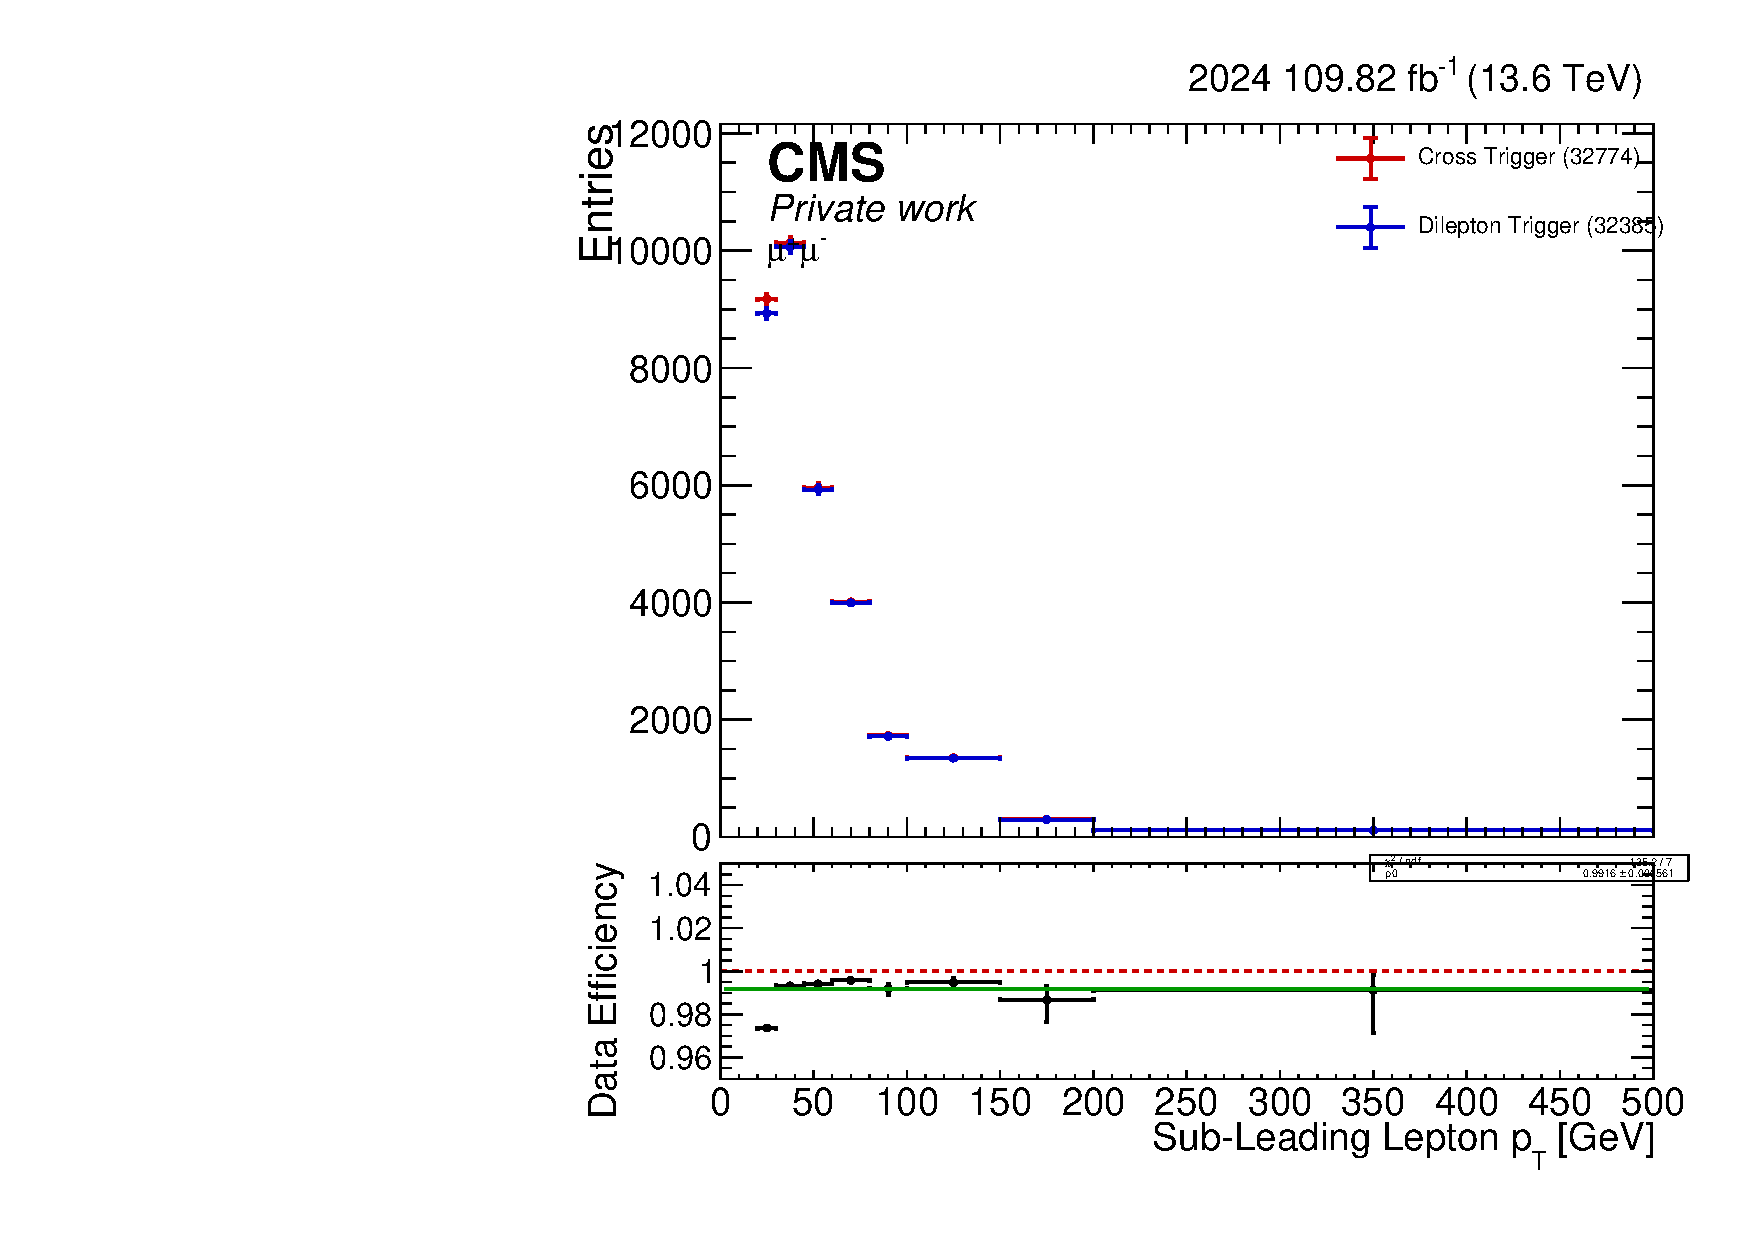
\includegraphics[width=0.48\linewidth]{figures/2024/MuMu/TrigEffData/TrigEff_Lep2pt.pdf}
\caption{Data trigger numerator and reference-sample distributions (upper panels), with their efficiency ratios (lower panels) in the $\mu\mu$ channel. Left and right: leading and subleading lepton $p_{\mathrm{T}}$.}\label{fig:extra-MuMu-TrigEffData-Lep1pt}\end{figure}
\begin{figure}[p]\centering
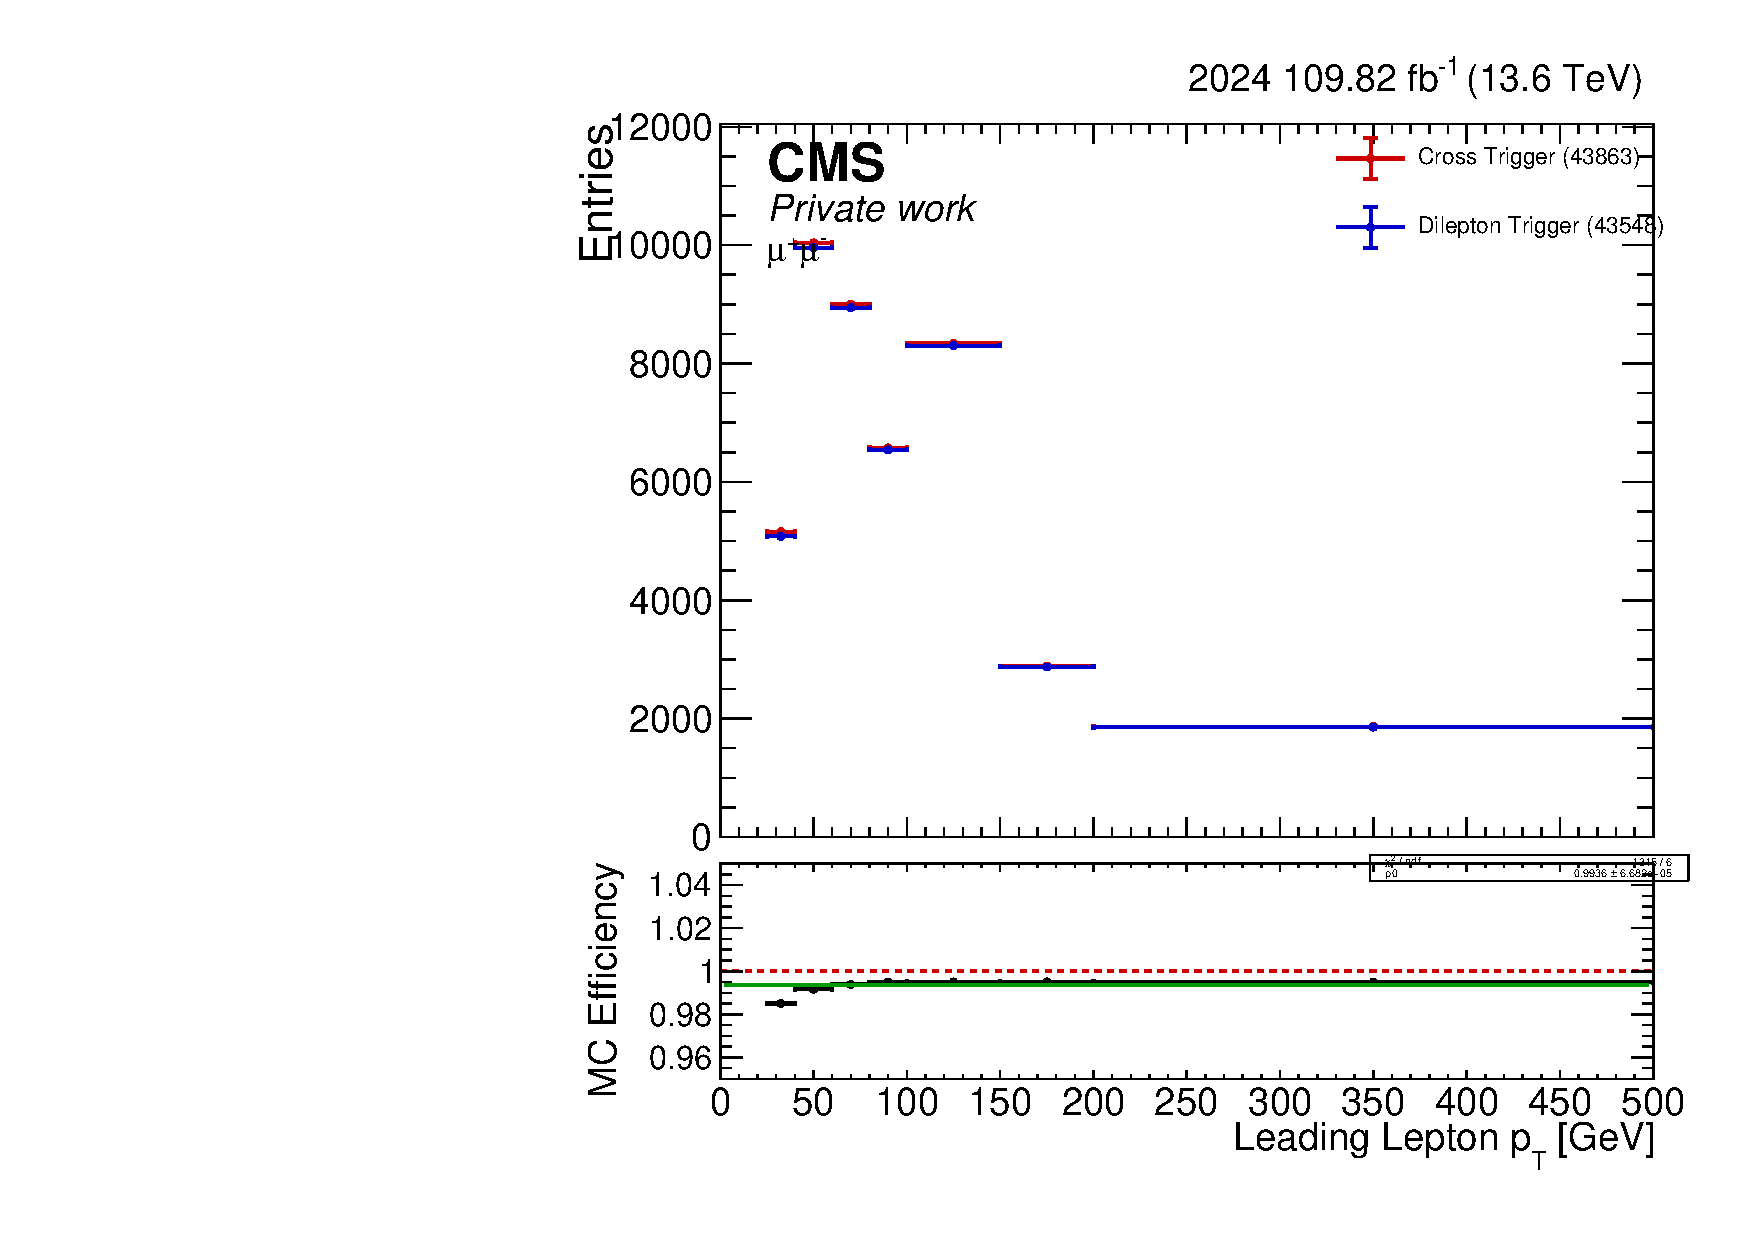
\includegraphics[width=0.48\linewidth]{figures/2024/MuMu/TrigEffMC/TrigEff_Lep1pt.pdf}
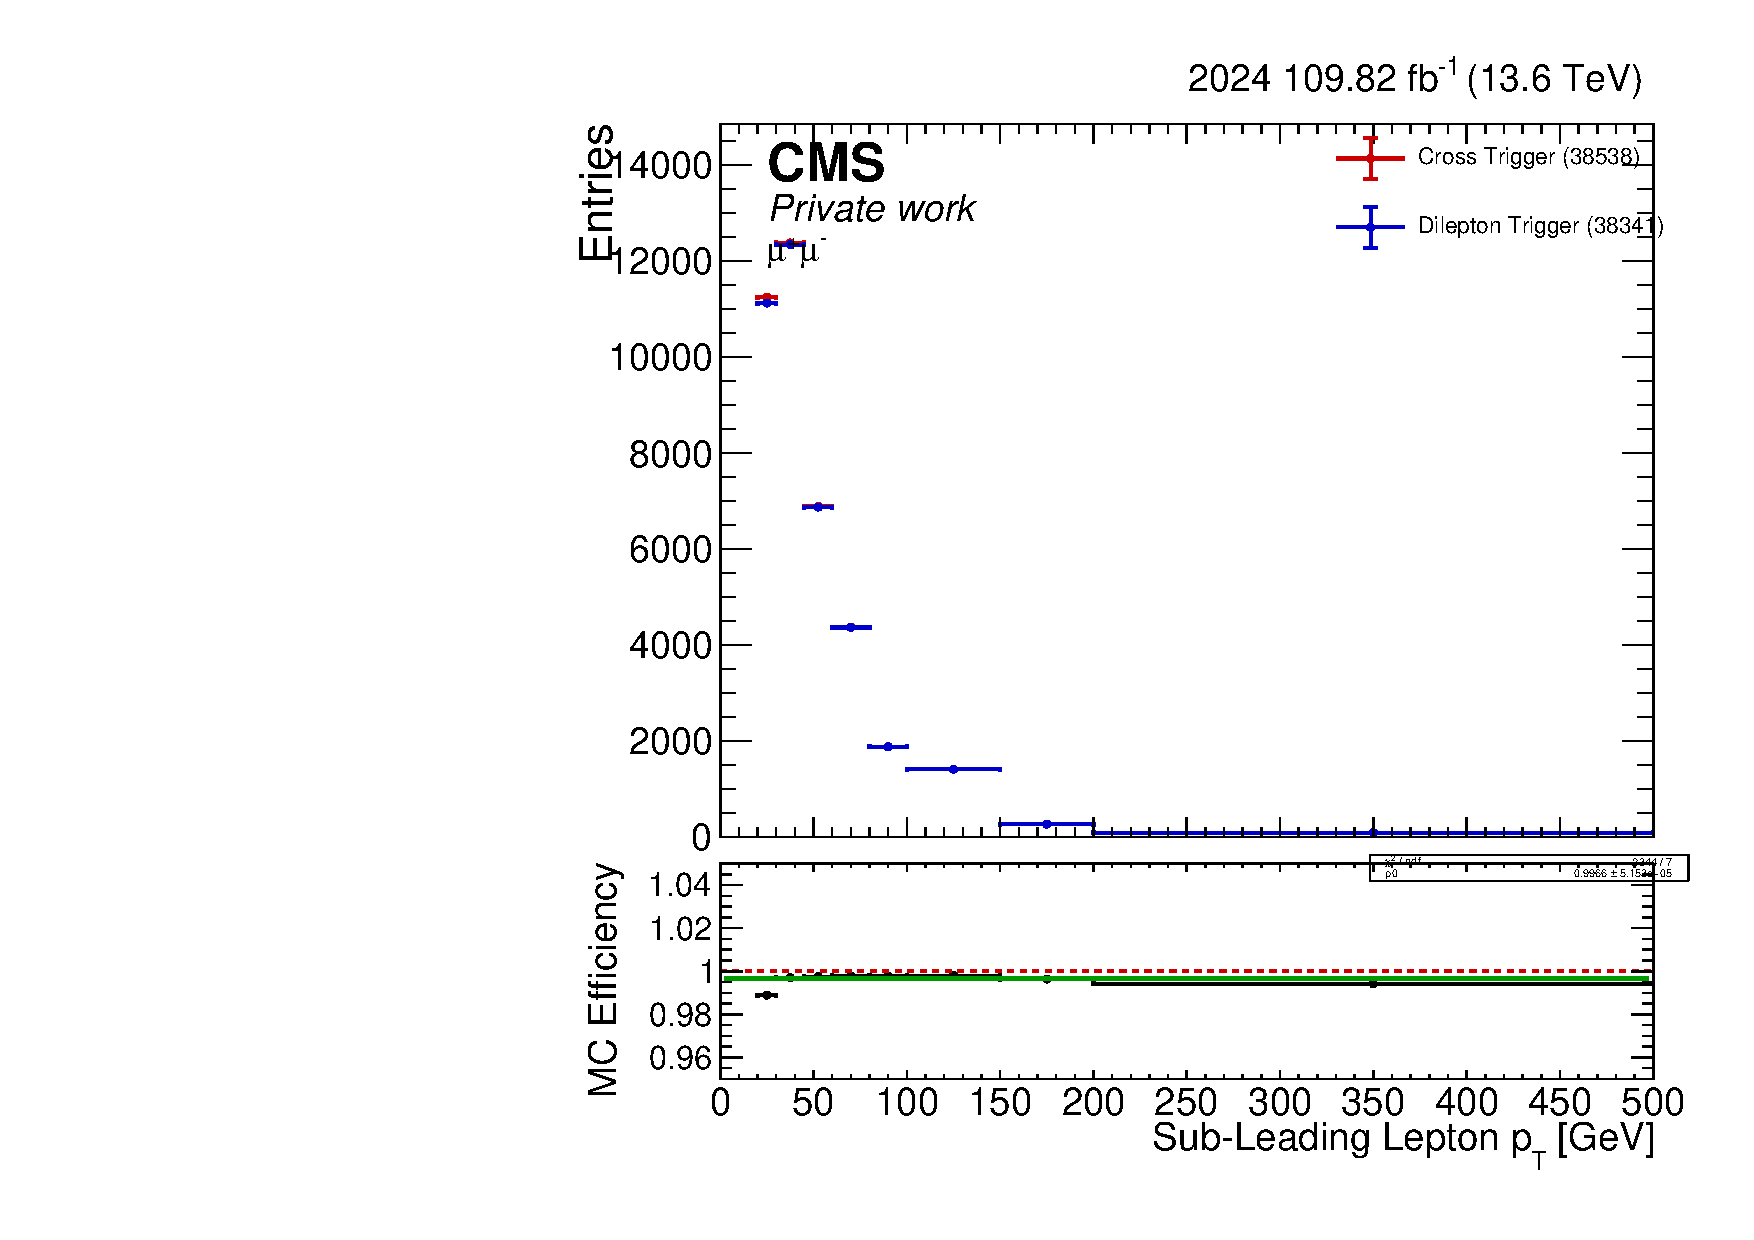
\includegraphics[width=0.48\linewidth]{figures/2024/MuMu/TrigEffMC/TrigEff_Lep2pt.pdf}
\caption{Simulated trigger numerator and reference-sample distributions (upper panels), with their efficiency ratios (lower panels) in the $\mu\mu$ channel. Left and right: leading and subleading lepton $p_{\mathrm{T}}$.}\label{fig:extra-MuMu-TrigEffMC-Lep1pt}\end{figure}
\begin{figure}[p]\centering
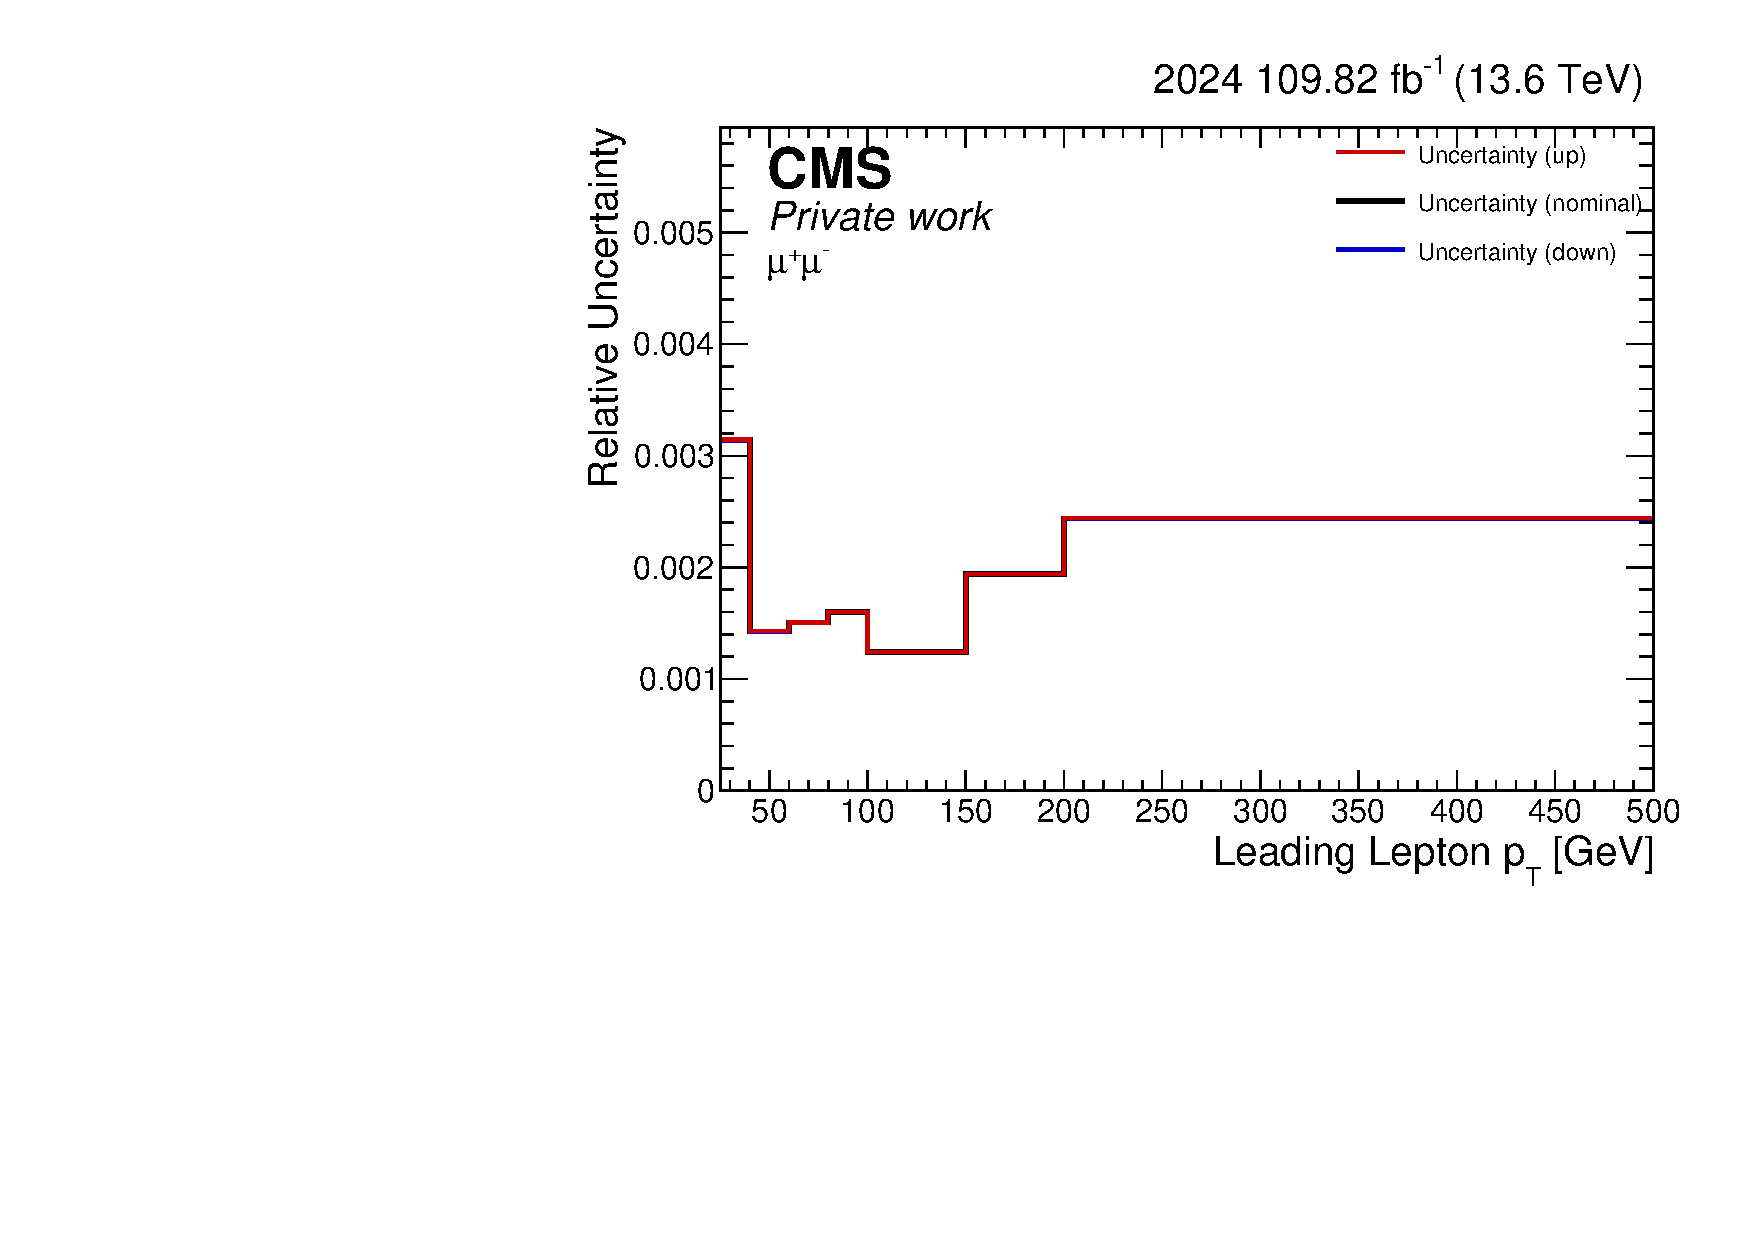
\includegraphics[width=0.48\linewidth]{figures/2024/MuMu/Statistical_Uncertainty/UncRatio_Lep1pt.pdf}
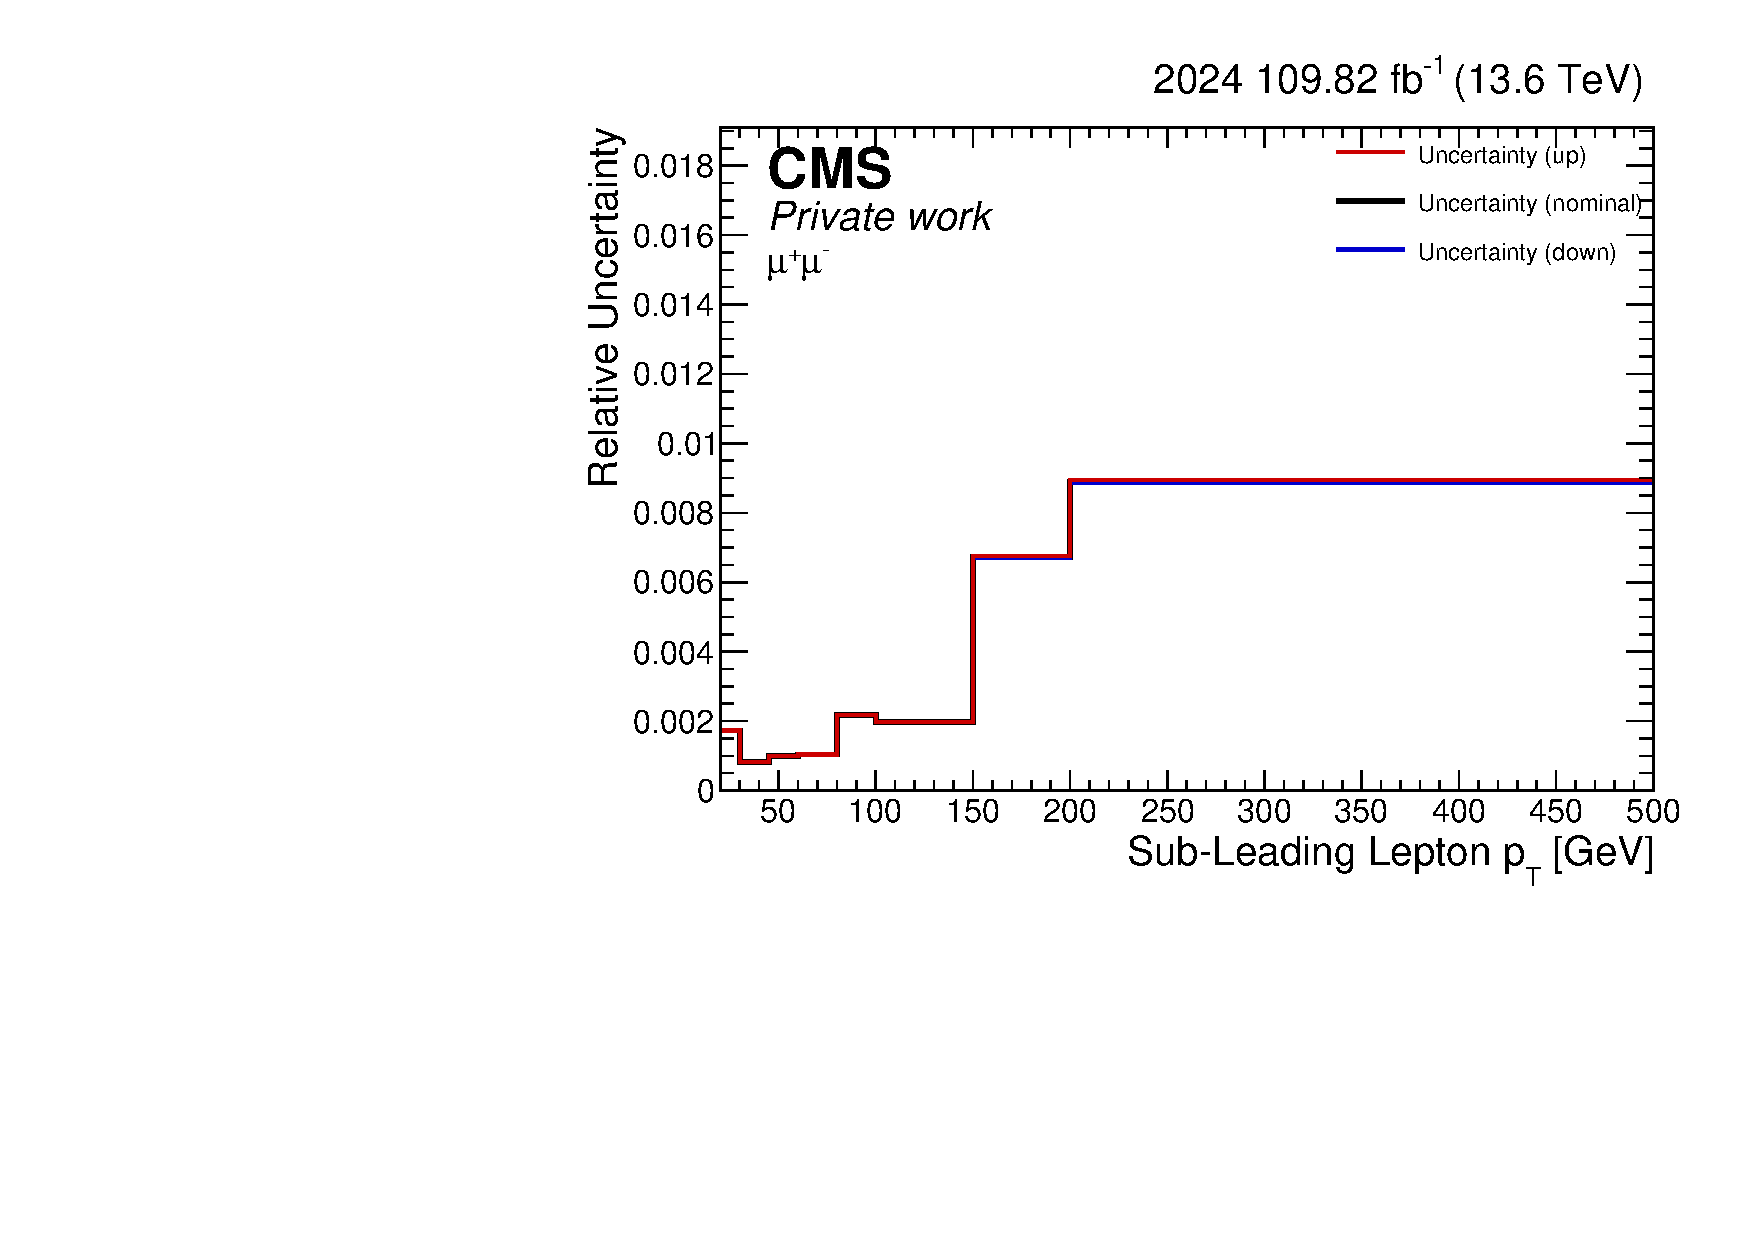
\includegraphics[width=0.48\linewidth]{figures/2024/MuMu/Statistical_Uncertainty/UncRatio_Lep2pt.pdf}
\caption{Relative statistical uncertainty diagnostics, retaining the nominal, upward, and downward curves of the supplied production in the $\mu\mu$ channel. Left and right: leading and subleading lepton $p_{\mathrm{T}}$.}\label{fig:extra-MuMu-Statistical-Uncertainty-Lep1pt}\end{figure}
\begin{figure}[p]\centering
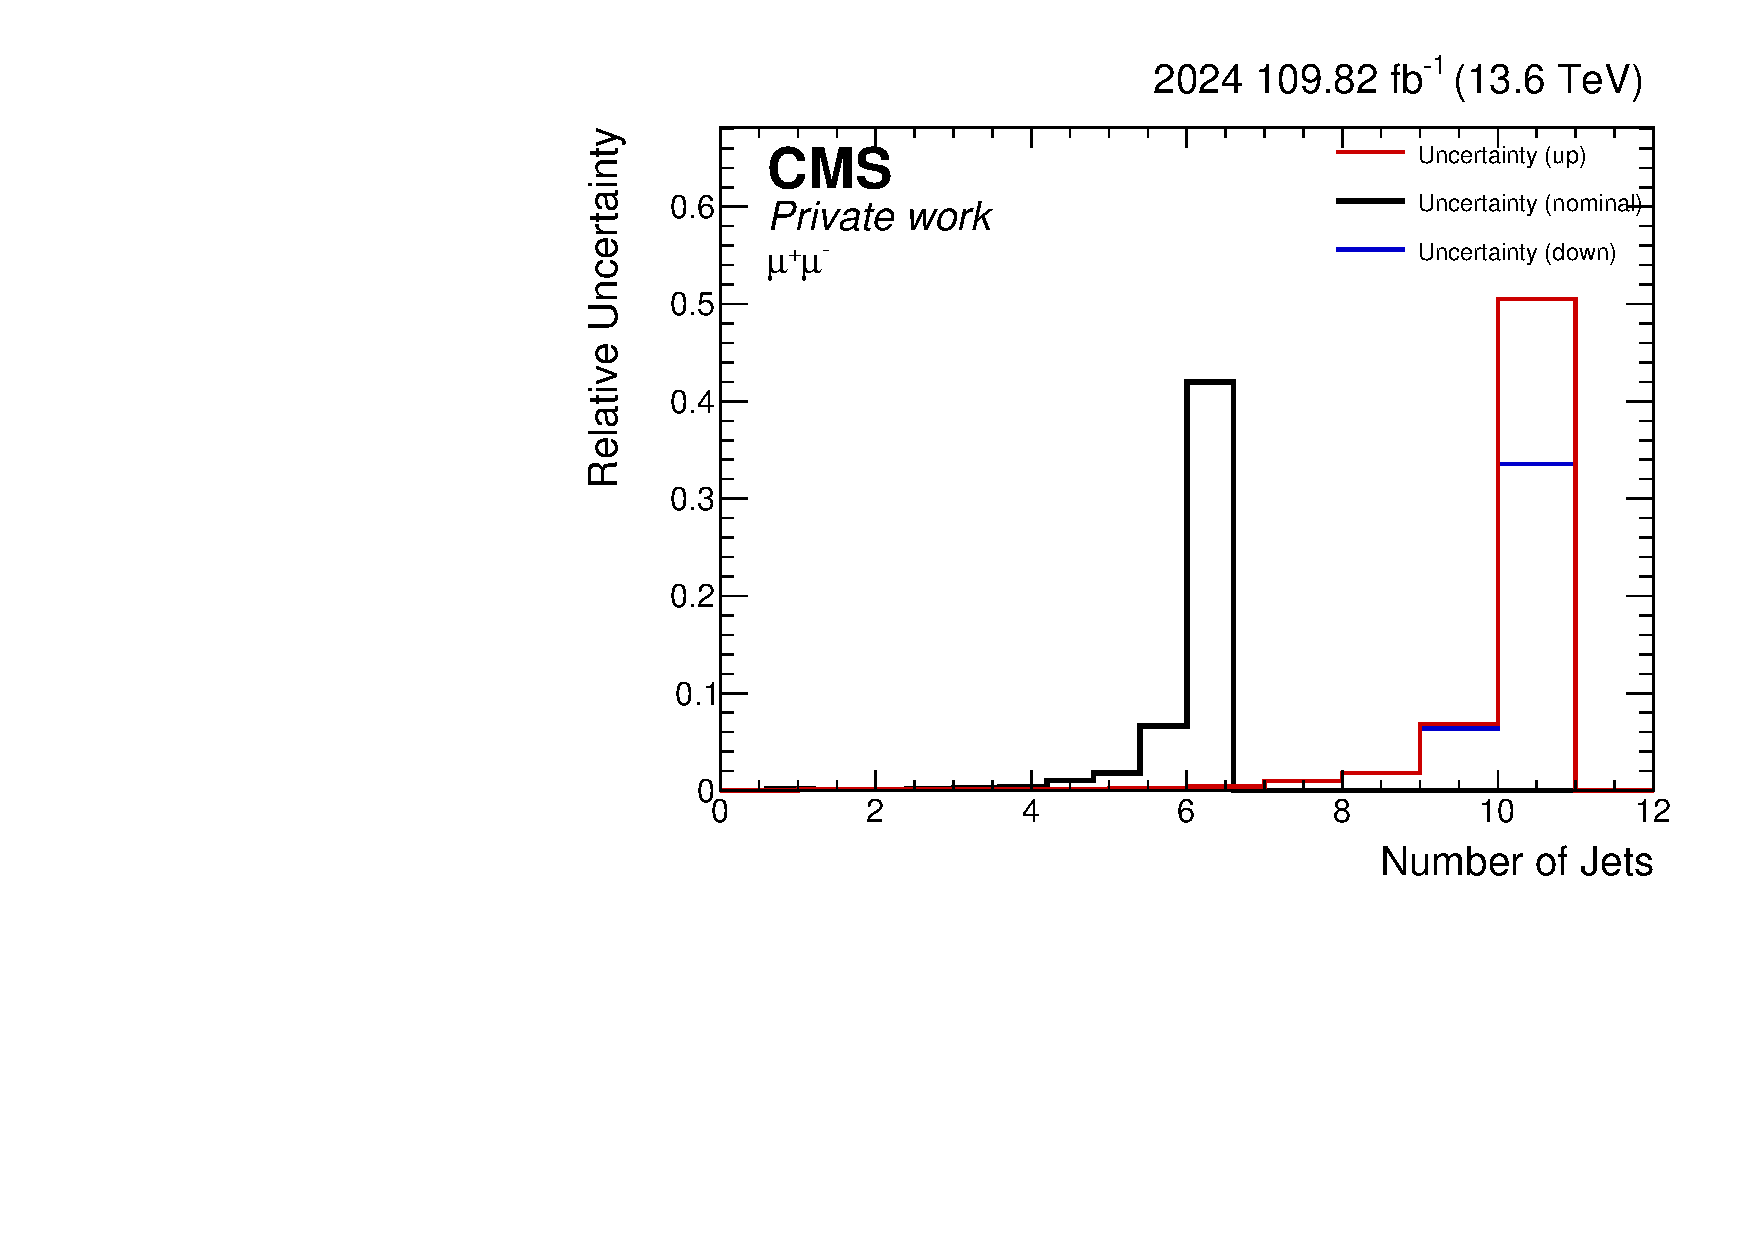
\includegraphics[width=0.48\linewidth]{figures/2024/MuMu/Statistical_Uncertainty/UncRatio_Num_Jets.pdf}
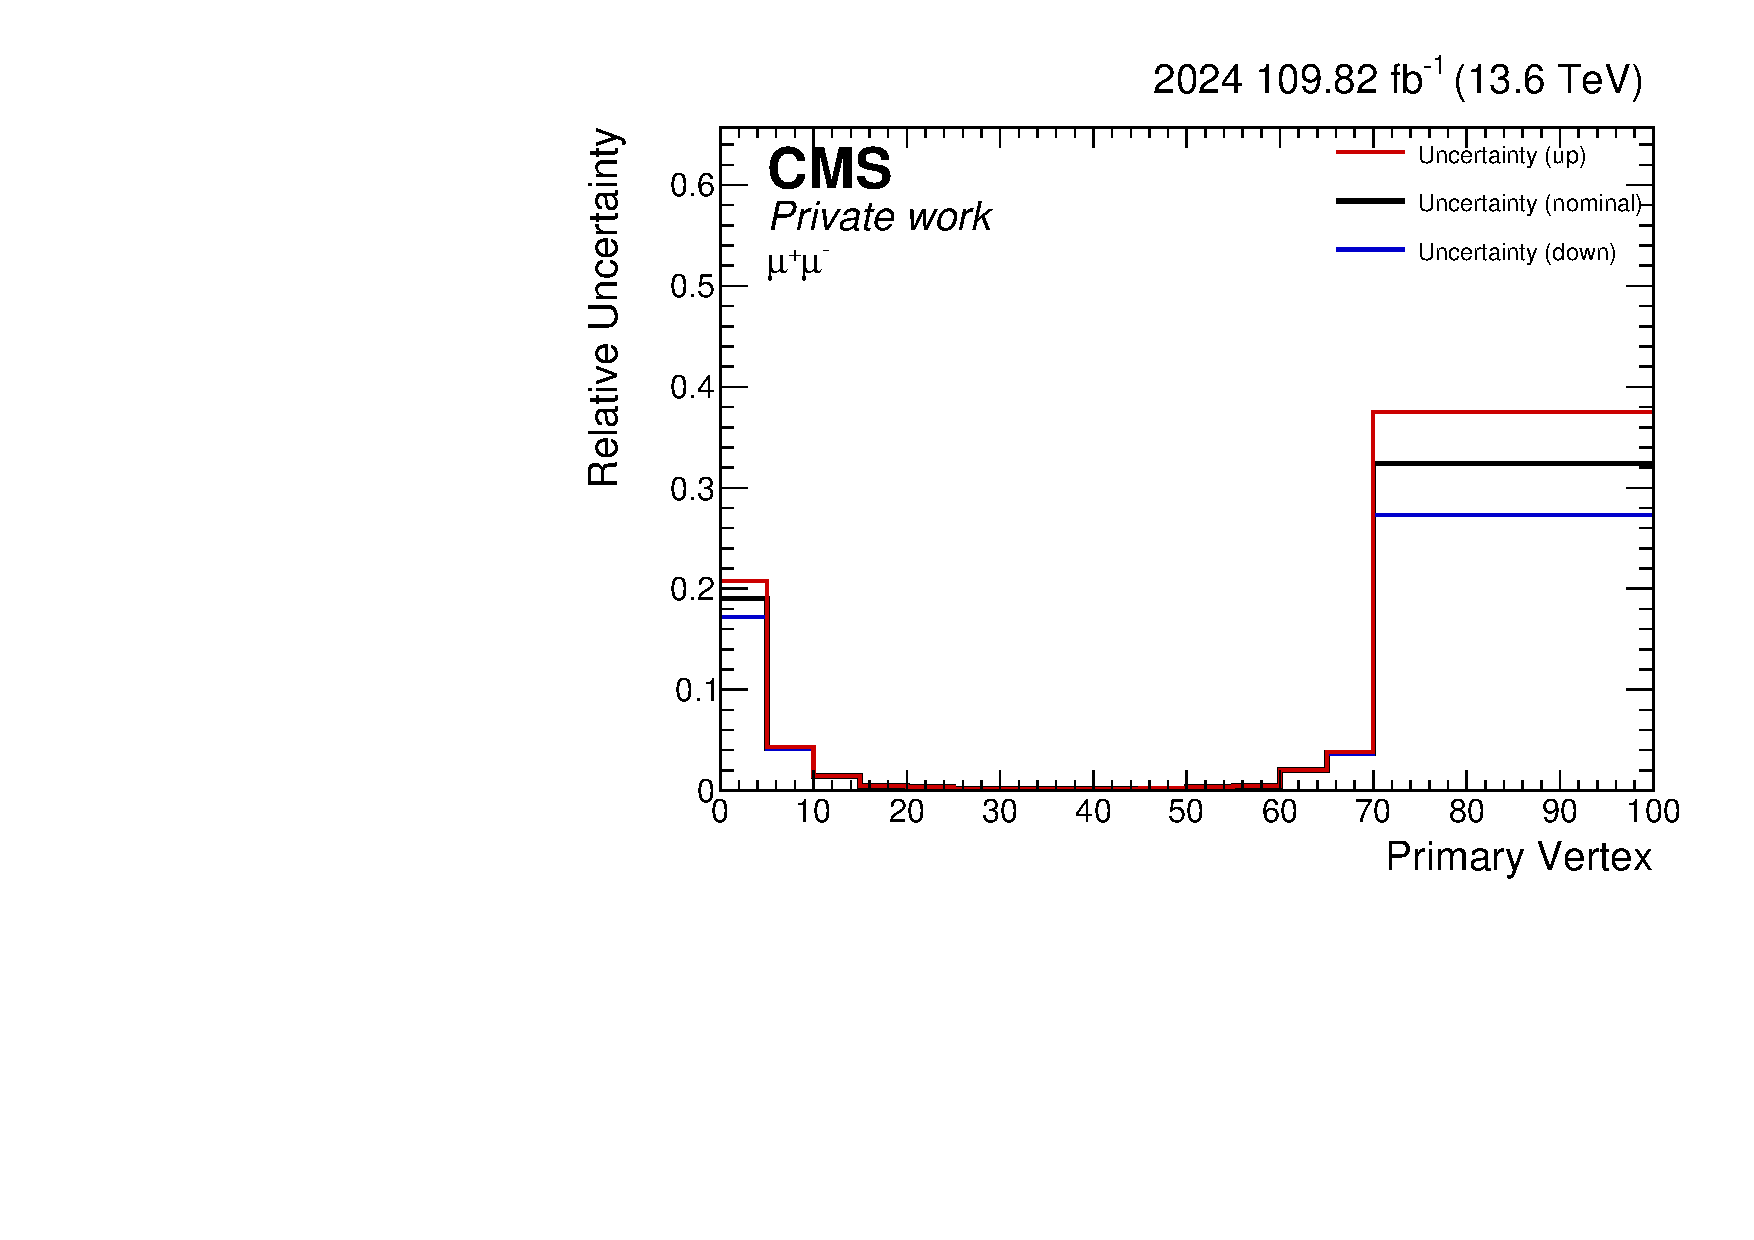
\includegraphics[width=0.48\linewidth]{figures/2024/MuMu/Statistical_Uncertainty/UncRatio_Num_PV.pdf}
\caption{Relative statistical uncertainty diagnostics, retaining the nominal, upward, and downward curves of the supplied production in the $\mu\mu$ channel. Left and right: jet and primary-vertex multiplicities.}\label{fig:extra-MuMu-Statistical-Uncertainty-Num_Jets}\end{figure}
\begin{figure}[p]\centering
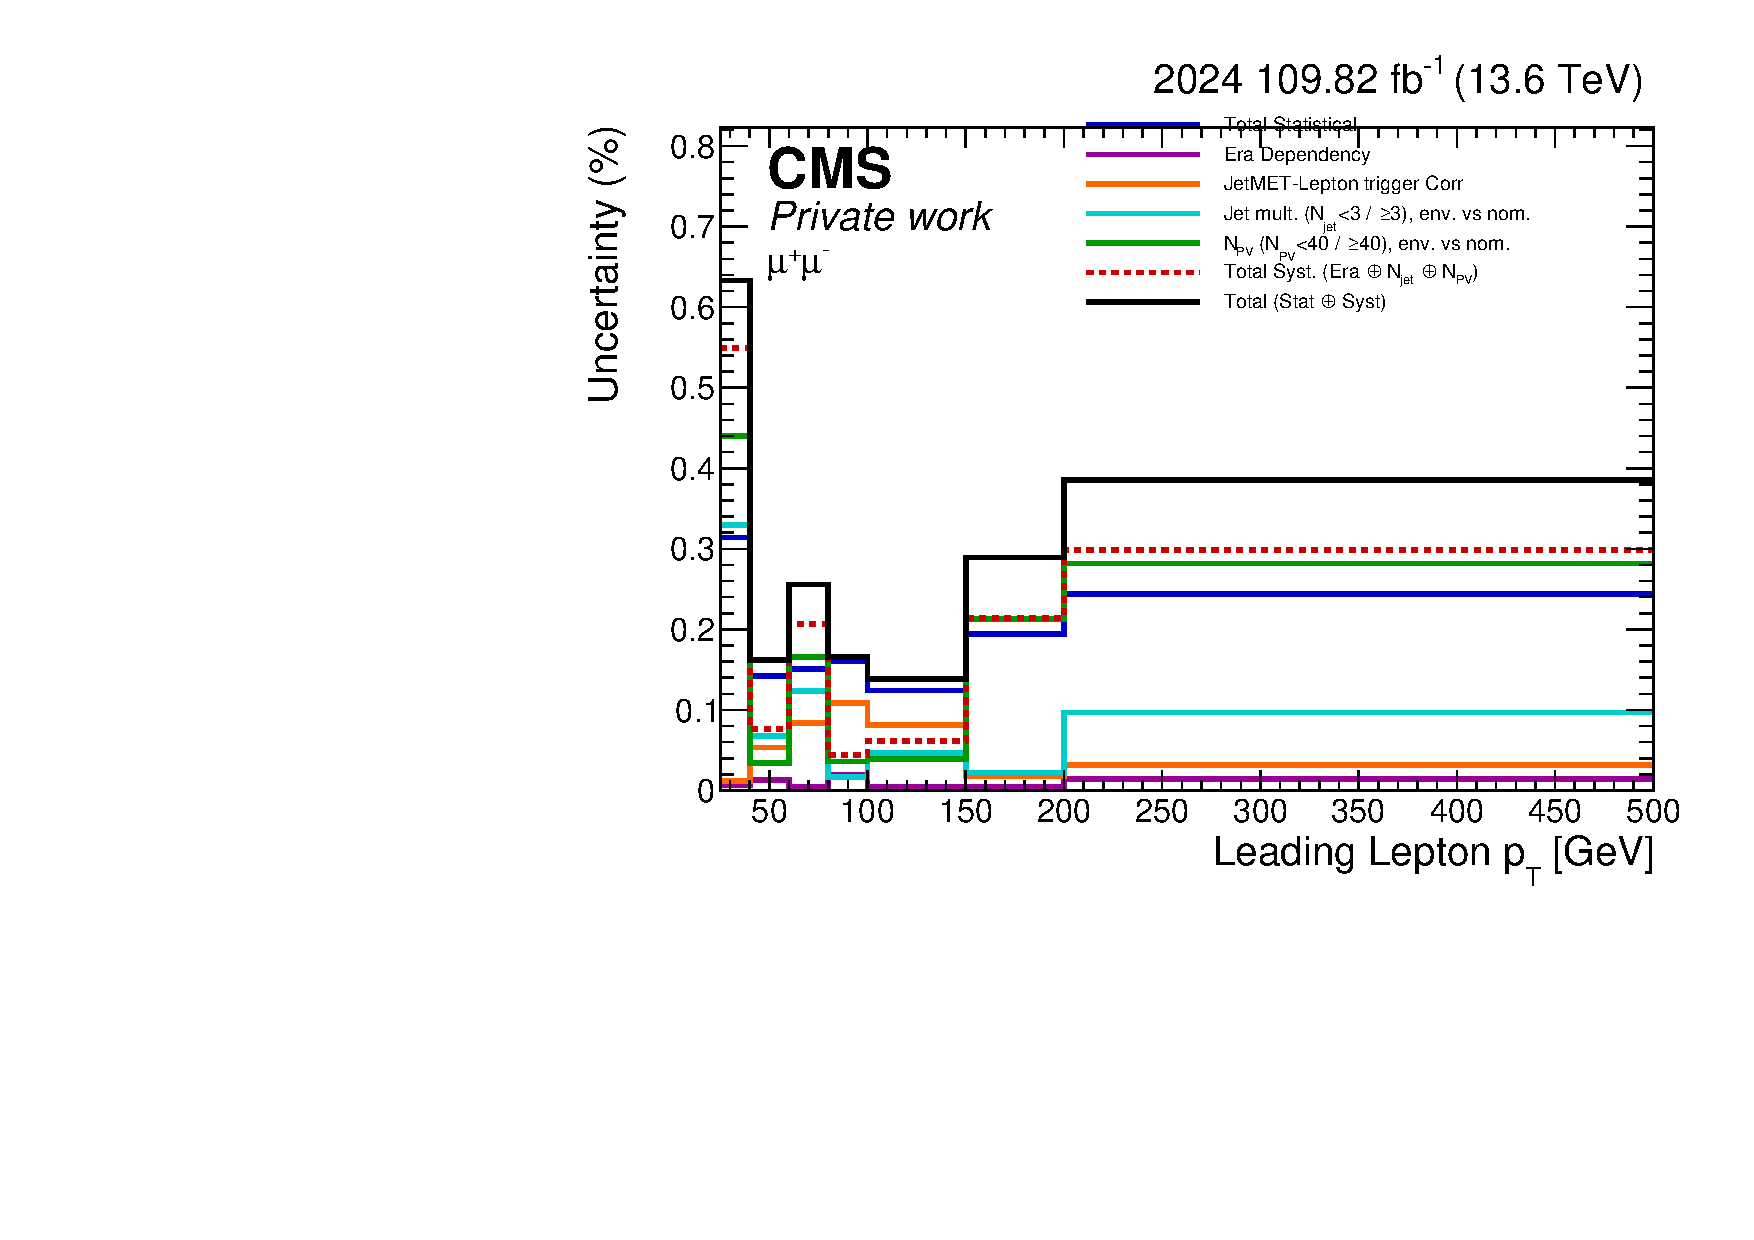
\includegraphics[width=0.48\linewidth]{figures/2024/MuMu/Uncertainty_Breakdown/Breakdown_Lep1pt.pdf}
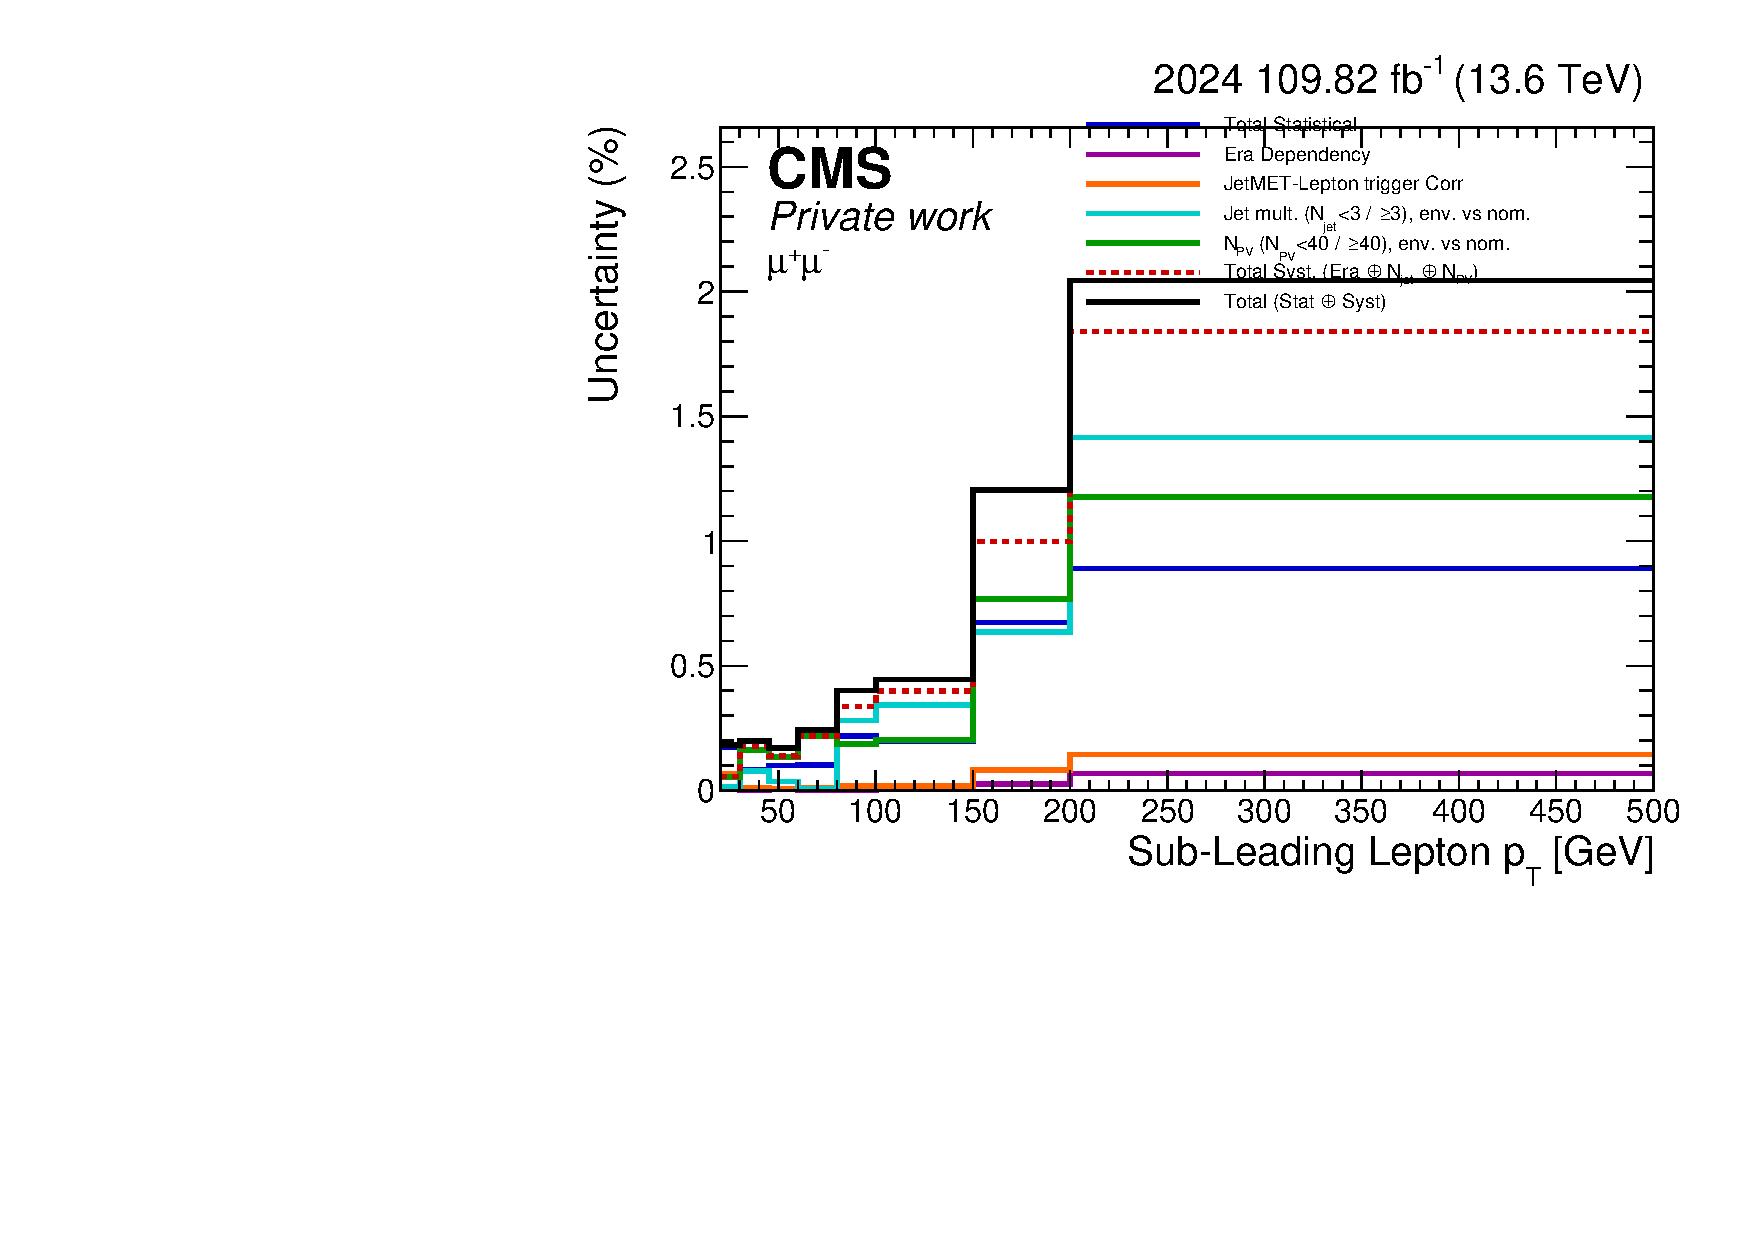
\includegraphics[width=0.48\linewidth]{figures/2024/MuMu/Uncertainty_Breakdown/Breakdown_Lep2pt.pdf}
\caption{Absolute uncertainty component breakdown in the $\mu\mu$ channel. Left and right: leading and subleading lepton $p_{\mathrm{T}}$.}\label{fig:extra-MuMu-Uncertainty-Breakdown-Lep1pt}\end{figure}
\begin{figure}[p]\centering
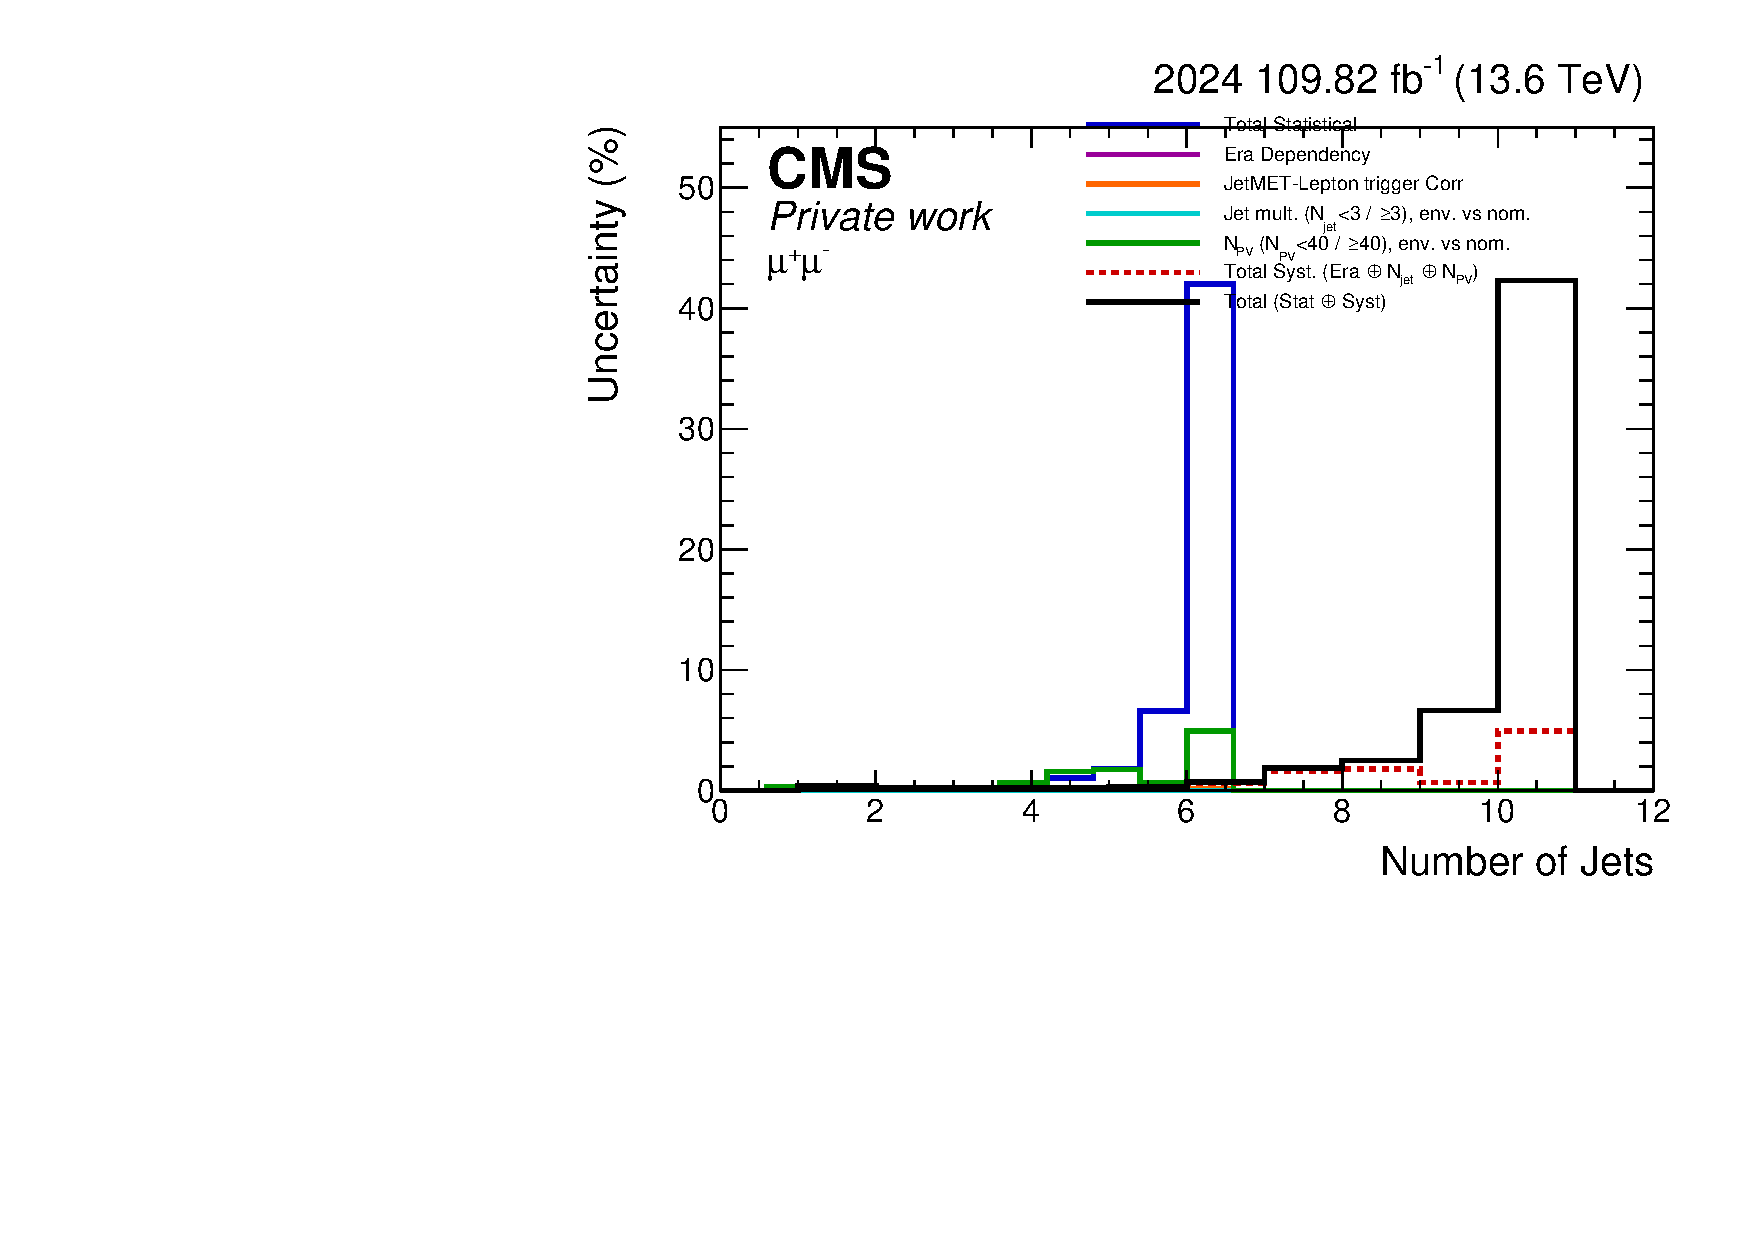
\includegraphics[width=0.48\linewidth]{figures/2024/MuMu/Uncertainty_Breakdown/Breakdown_Num_Jets.pdf}
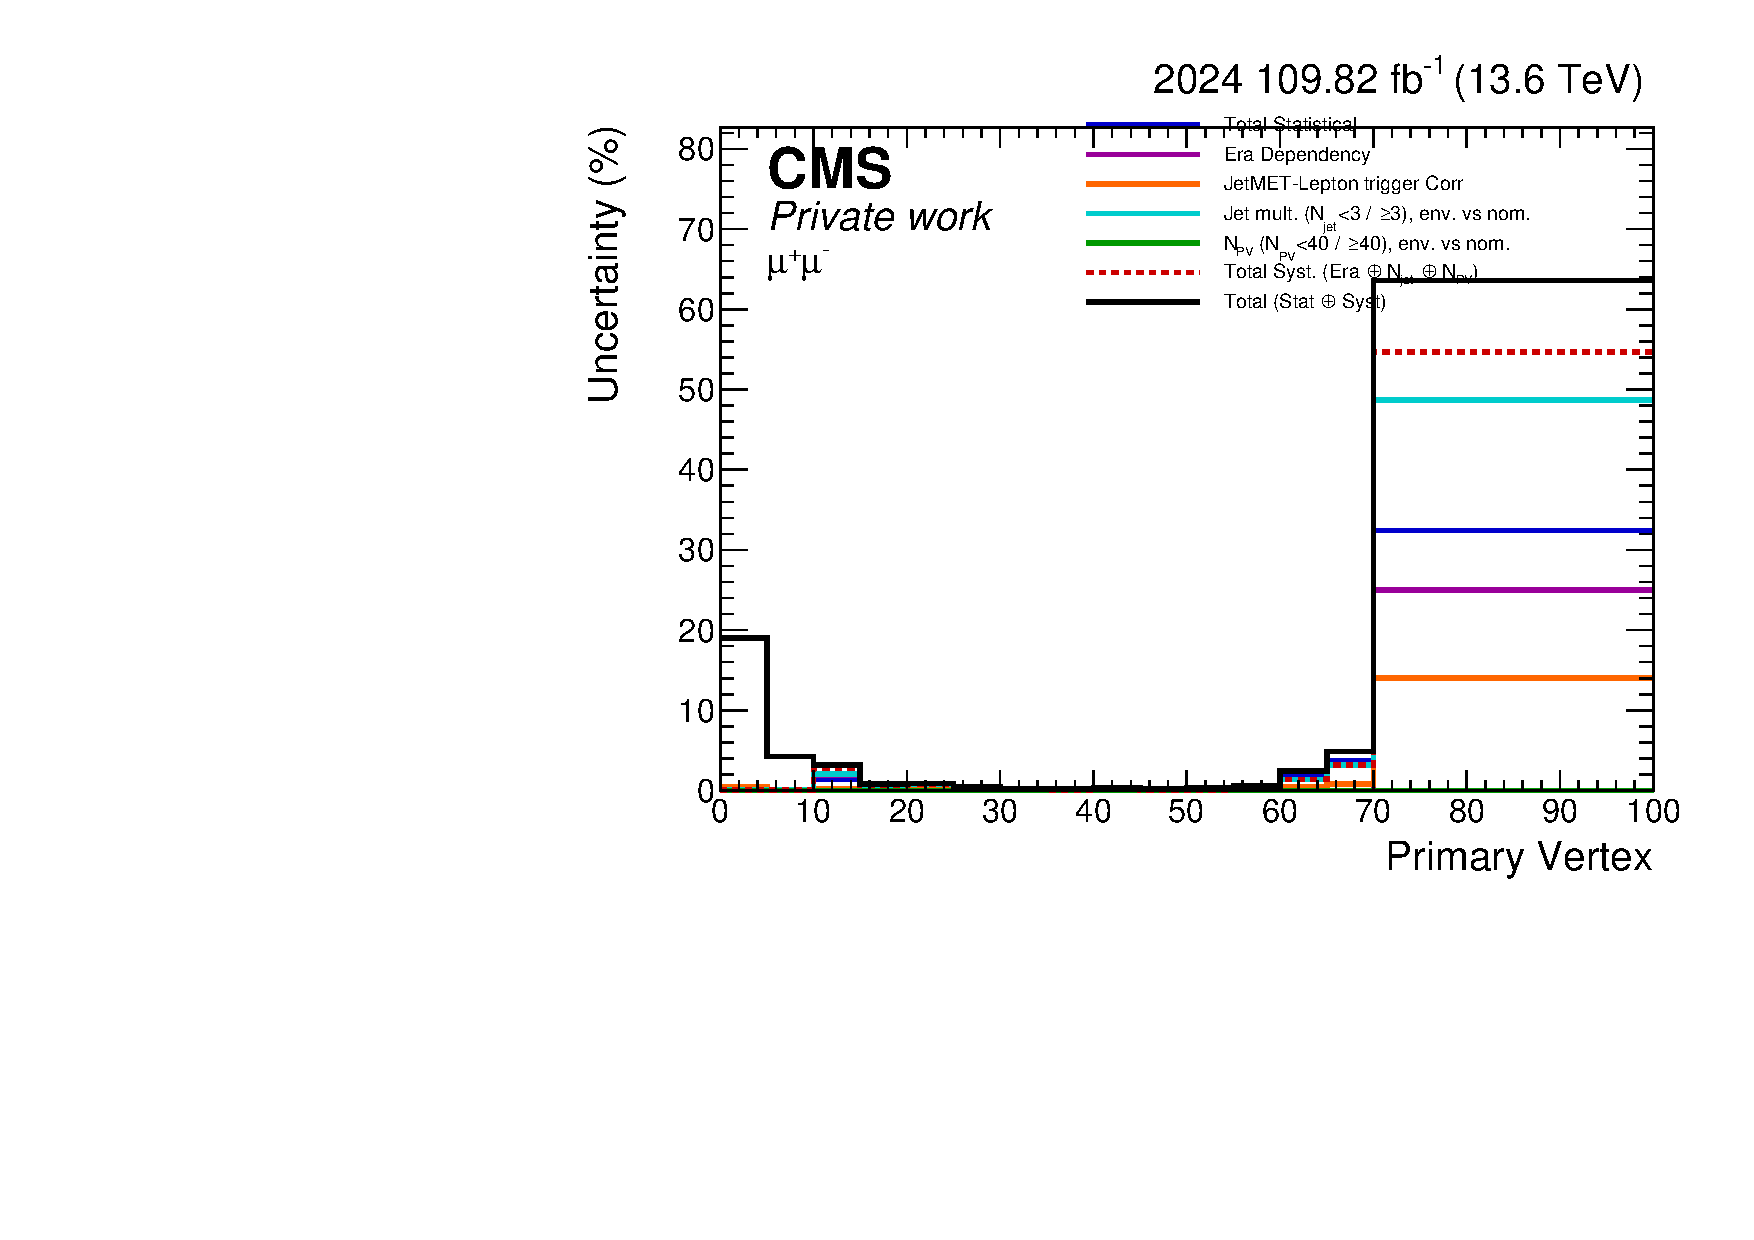
\includegraphics[width=0.48\linewidth]{figures/2024/MuMu/Uncertainty_Breakdown/Breakdown_Num_PV.pdf}
\caption{Absolute uncertainty component breakdown in the $\mu\mu$ channel. Left and right: jet and primary-vertex multiplicities.}\label{fig:extra-MuMu-Uncertainty-Breakdown-Num_Jets}\end{figure}
\begin{figure}[p]\centering
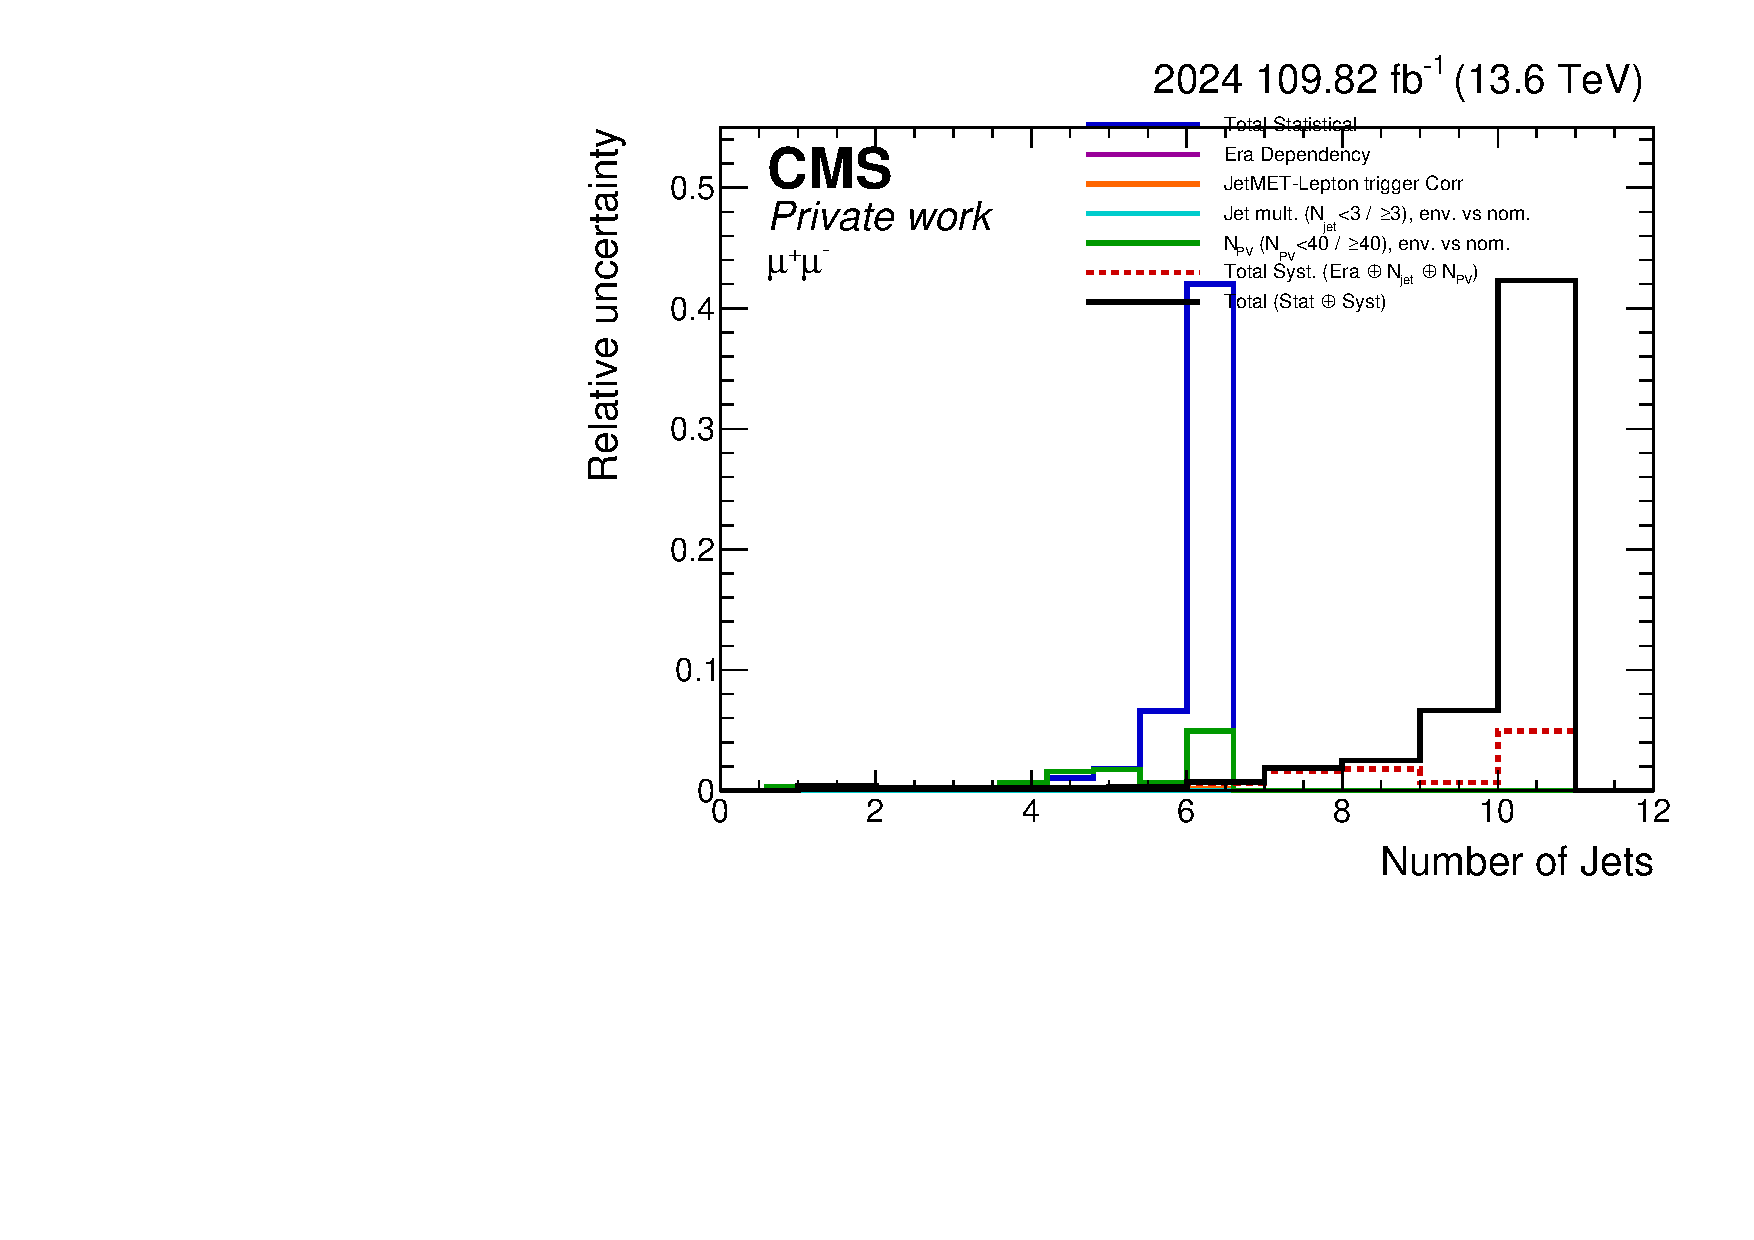
\includegraphics[width=0.48\linewidth]{figures/2024/MuMu/Relative_Uncertainty_Breakdown/Breakdown_Num_Jets.pdf}
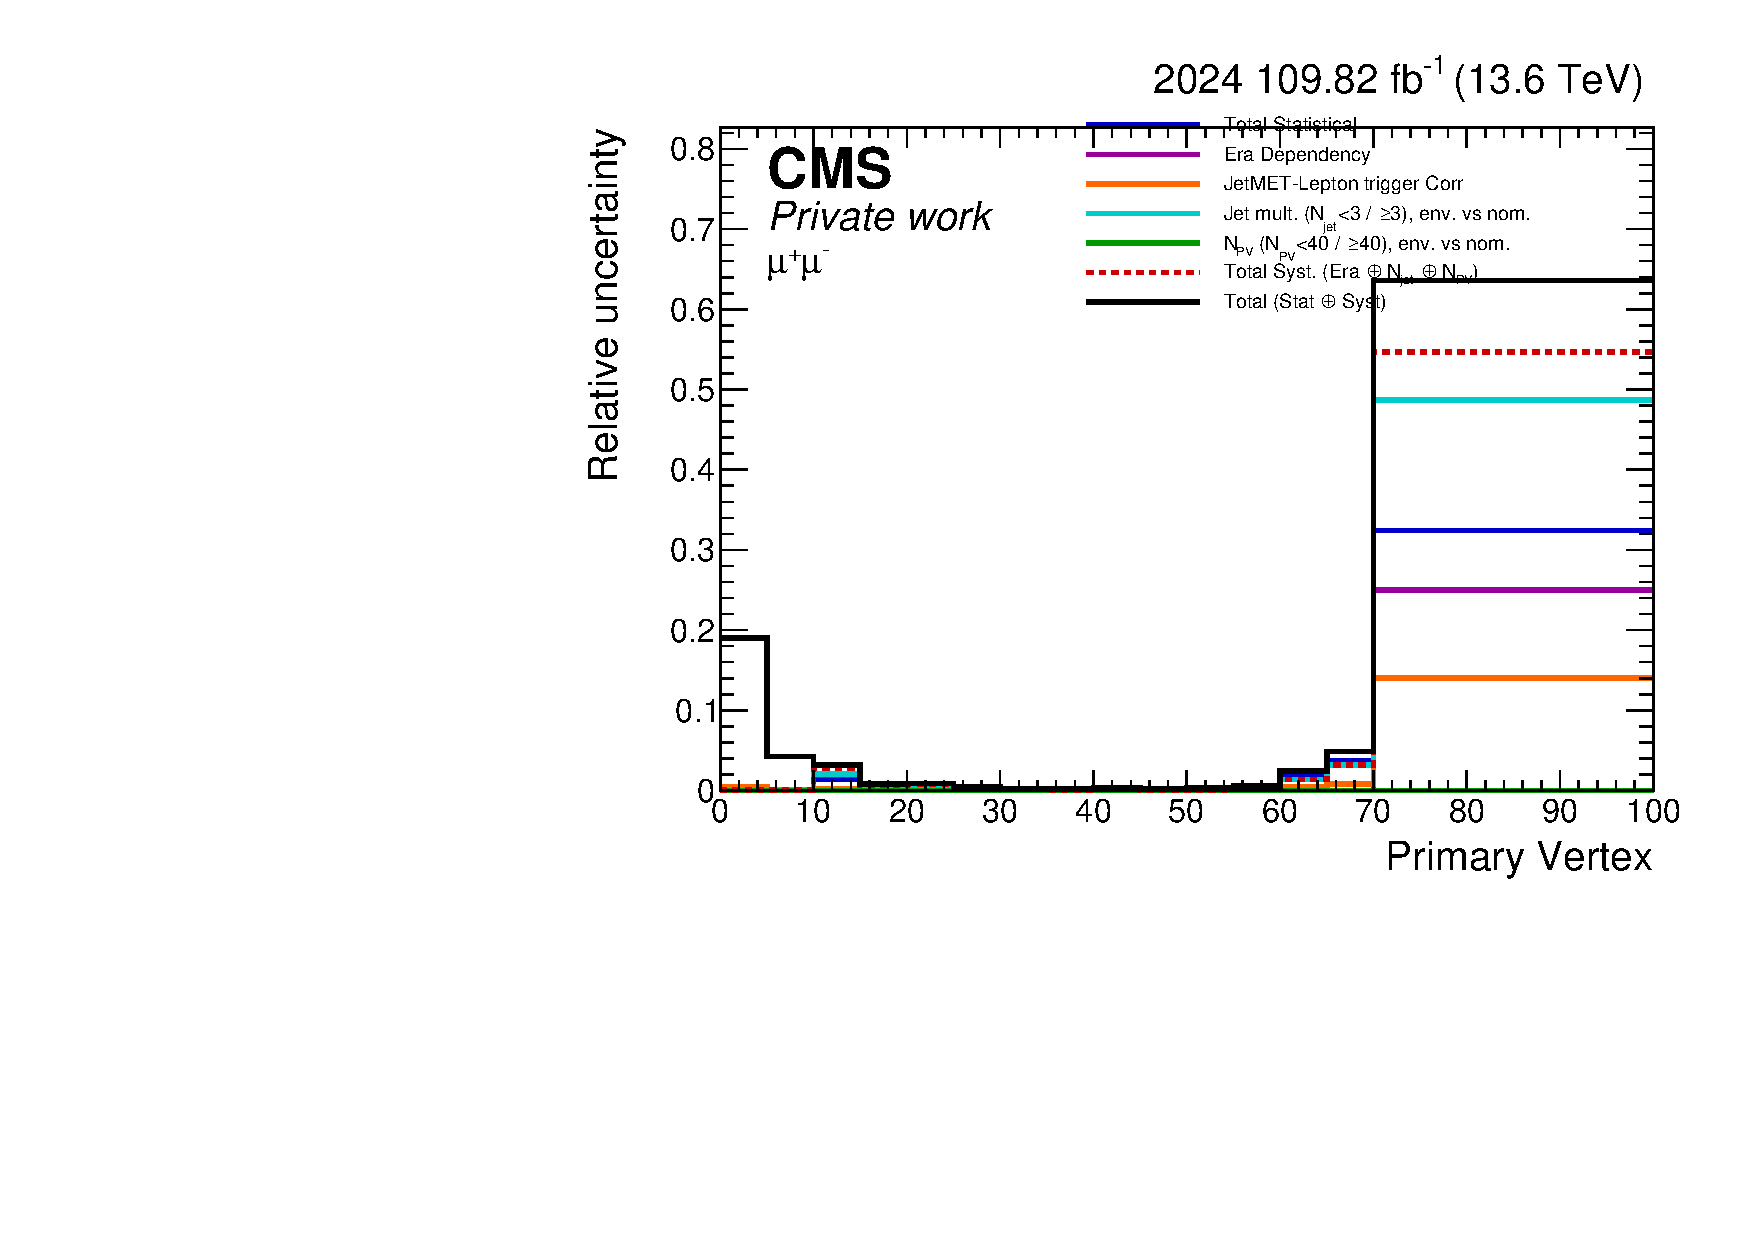
\includegraphics[width=0.48\linewidth]{figures/2024/MuMu/Relative_Uncertainty_Breakdown/Breakdown_Num_PV.pdf}
\caption{Relative uncertainty component breakdown versus event activity in the $\mu\mu$ channel. Left and right: jet and primary-vertex multiplicities.}\label{fig:extra-MuMu-Relative-Uncertainty-Breakdown-Num_Jets}\end{figure}
\begin{figure}[p]\centering
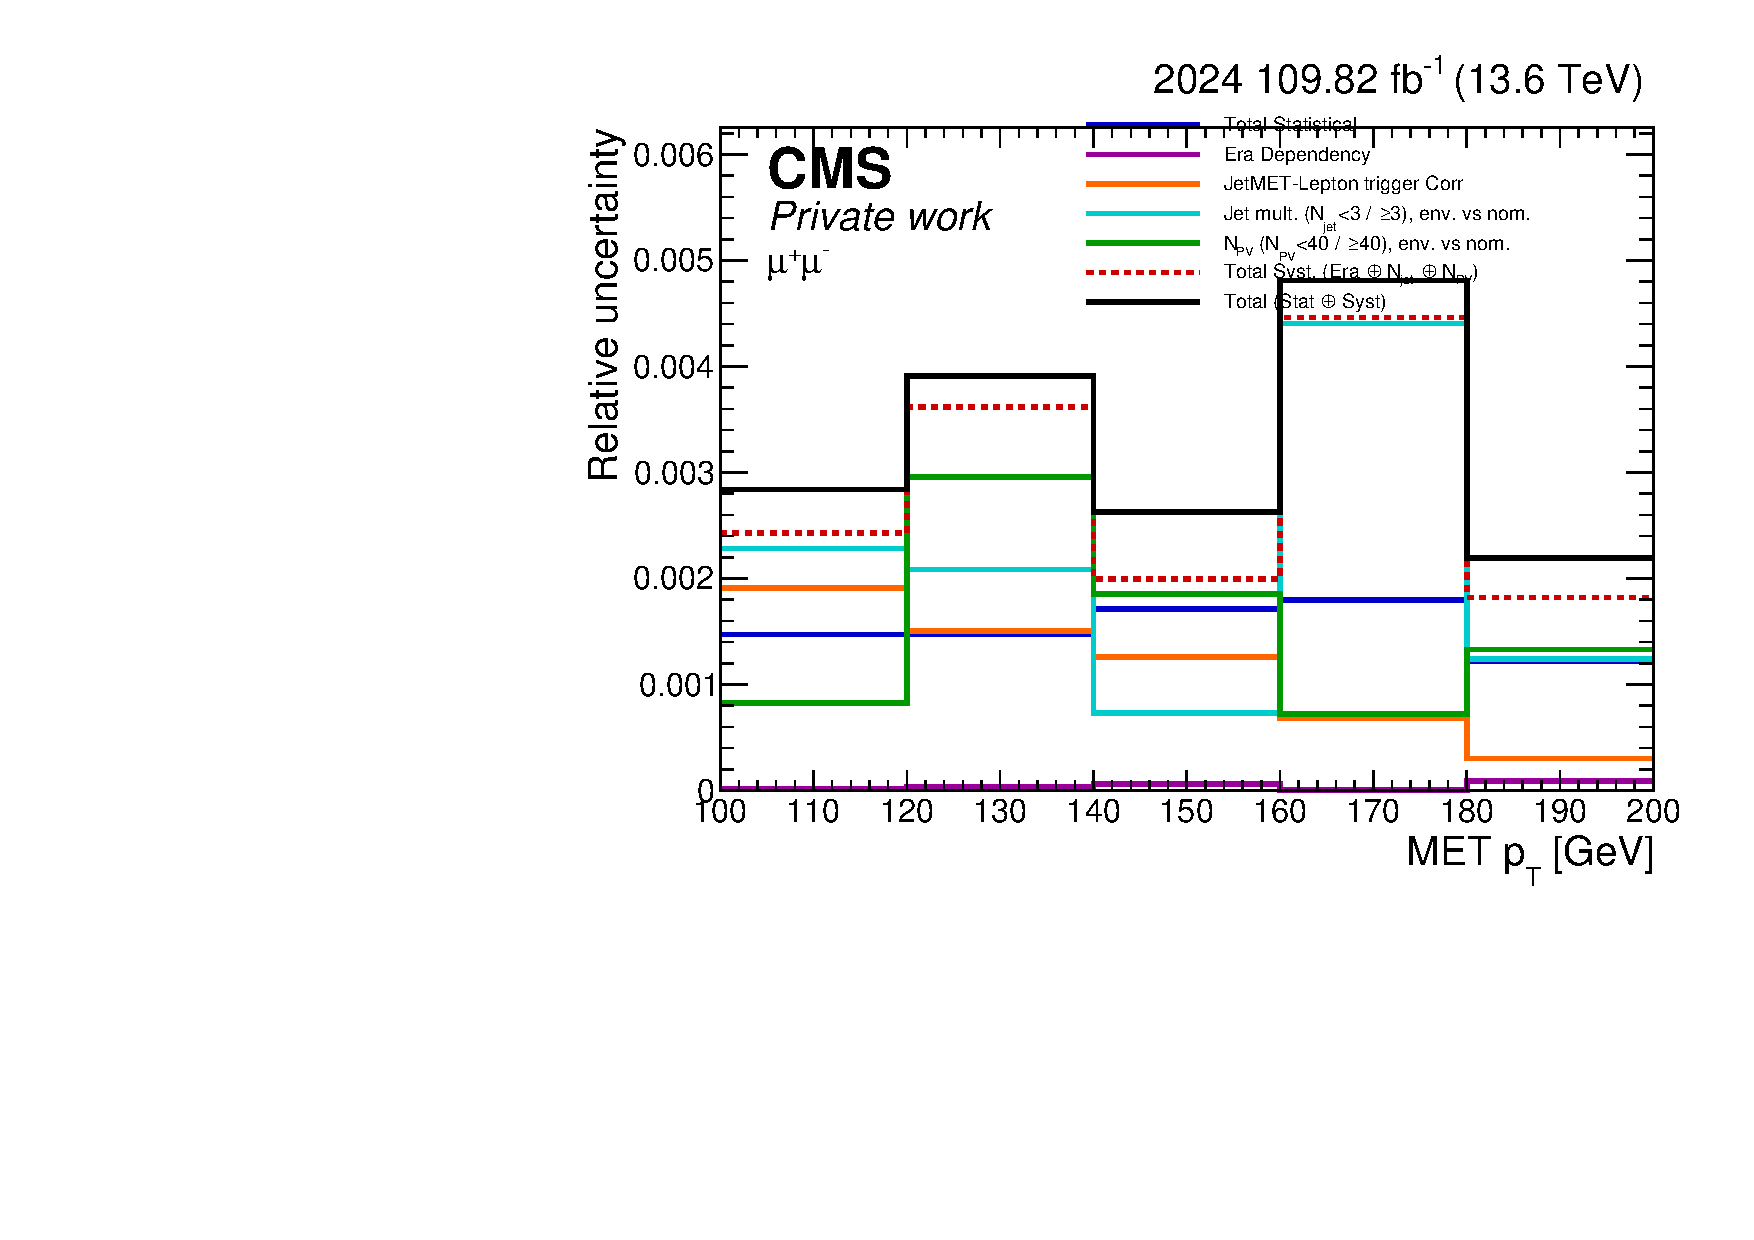
\includegraphics[width=0.48\linewidth]{figures/2024/MuMu/Relative_Uncertainty_Breakdown/Breakdown_METpt.pdf}
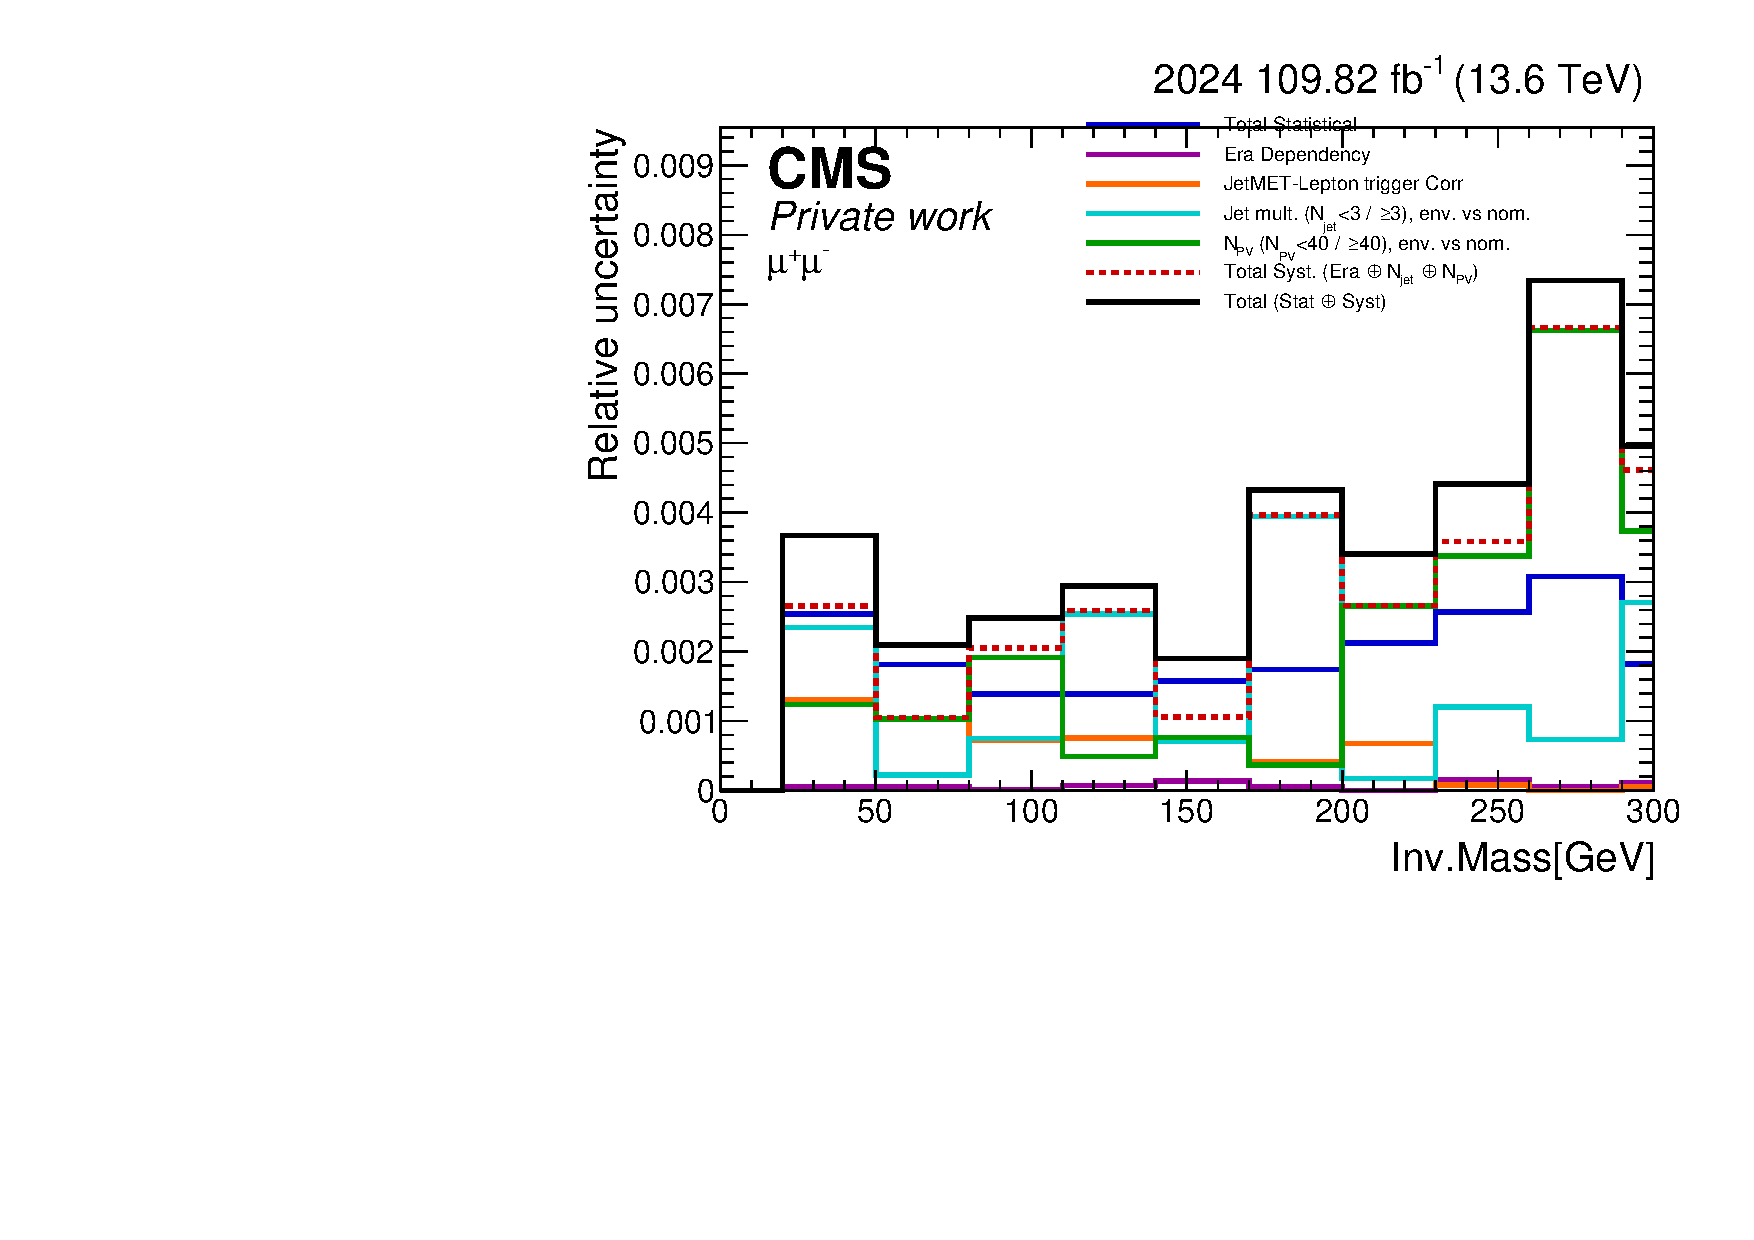
\includegraphics[width=0.48\linewidth]{figures/2024/MuMu/Relative_Uncertainty_Breakdown/Breakdown_DiLepMass.pdf}
\caption{Relative uncertainty component breakdown versus event kinematics in the $\mu\mu$ channel. Left and right: missing transverse momentum and dilepton invariant mass.}\label{fig:extra-MuMu-Relative-Uncertainty-Breakdown-METpt}\end{figure}
\begin{figure}[p]\centering
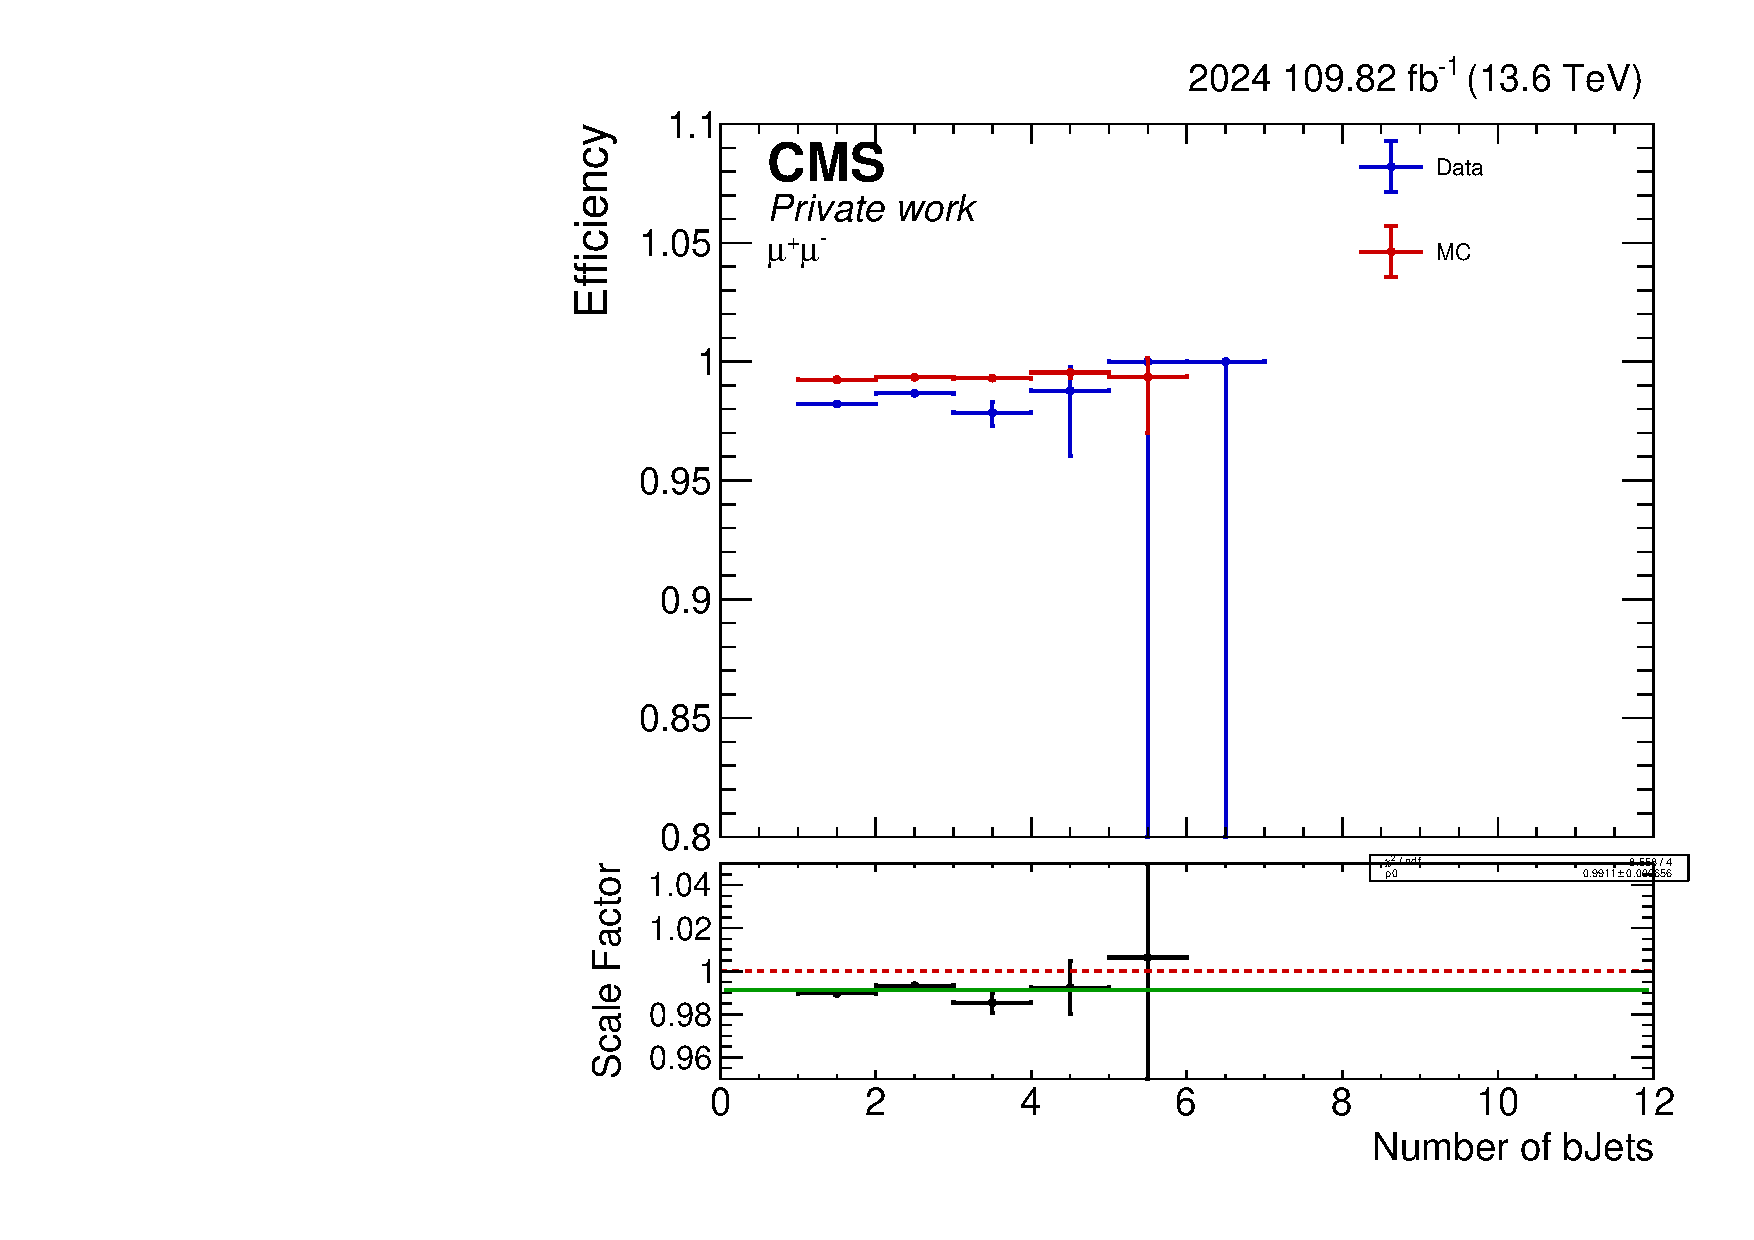
\includegraphics[width=0.48\linewidth]{figures/2024/MuMu/ScaleFactor/SF_Num_bJets.pdf}
\caption{Efficiency comparison and scale factor versus heavy-flavour activity in the $\mu\mu$ channel. $b$-tagged jet multiplicity.}\label{fig:extra-MuMu-ScaleFactor-Num_bJets}\end{figure}


\section{2025: additional kinematic dependence}\label{app:diagnostics-2025}
These distributions extend the main momentum comparisons. They use the same measurement sample and do not constitute independent closure tests.
\begin{figure}[htbp]\centering
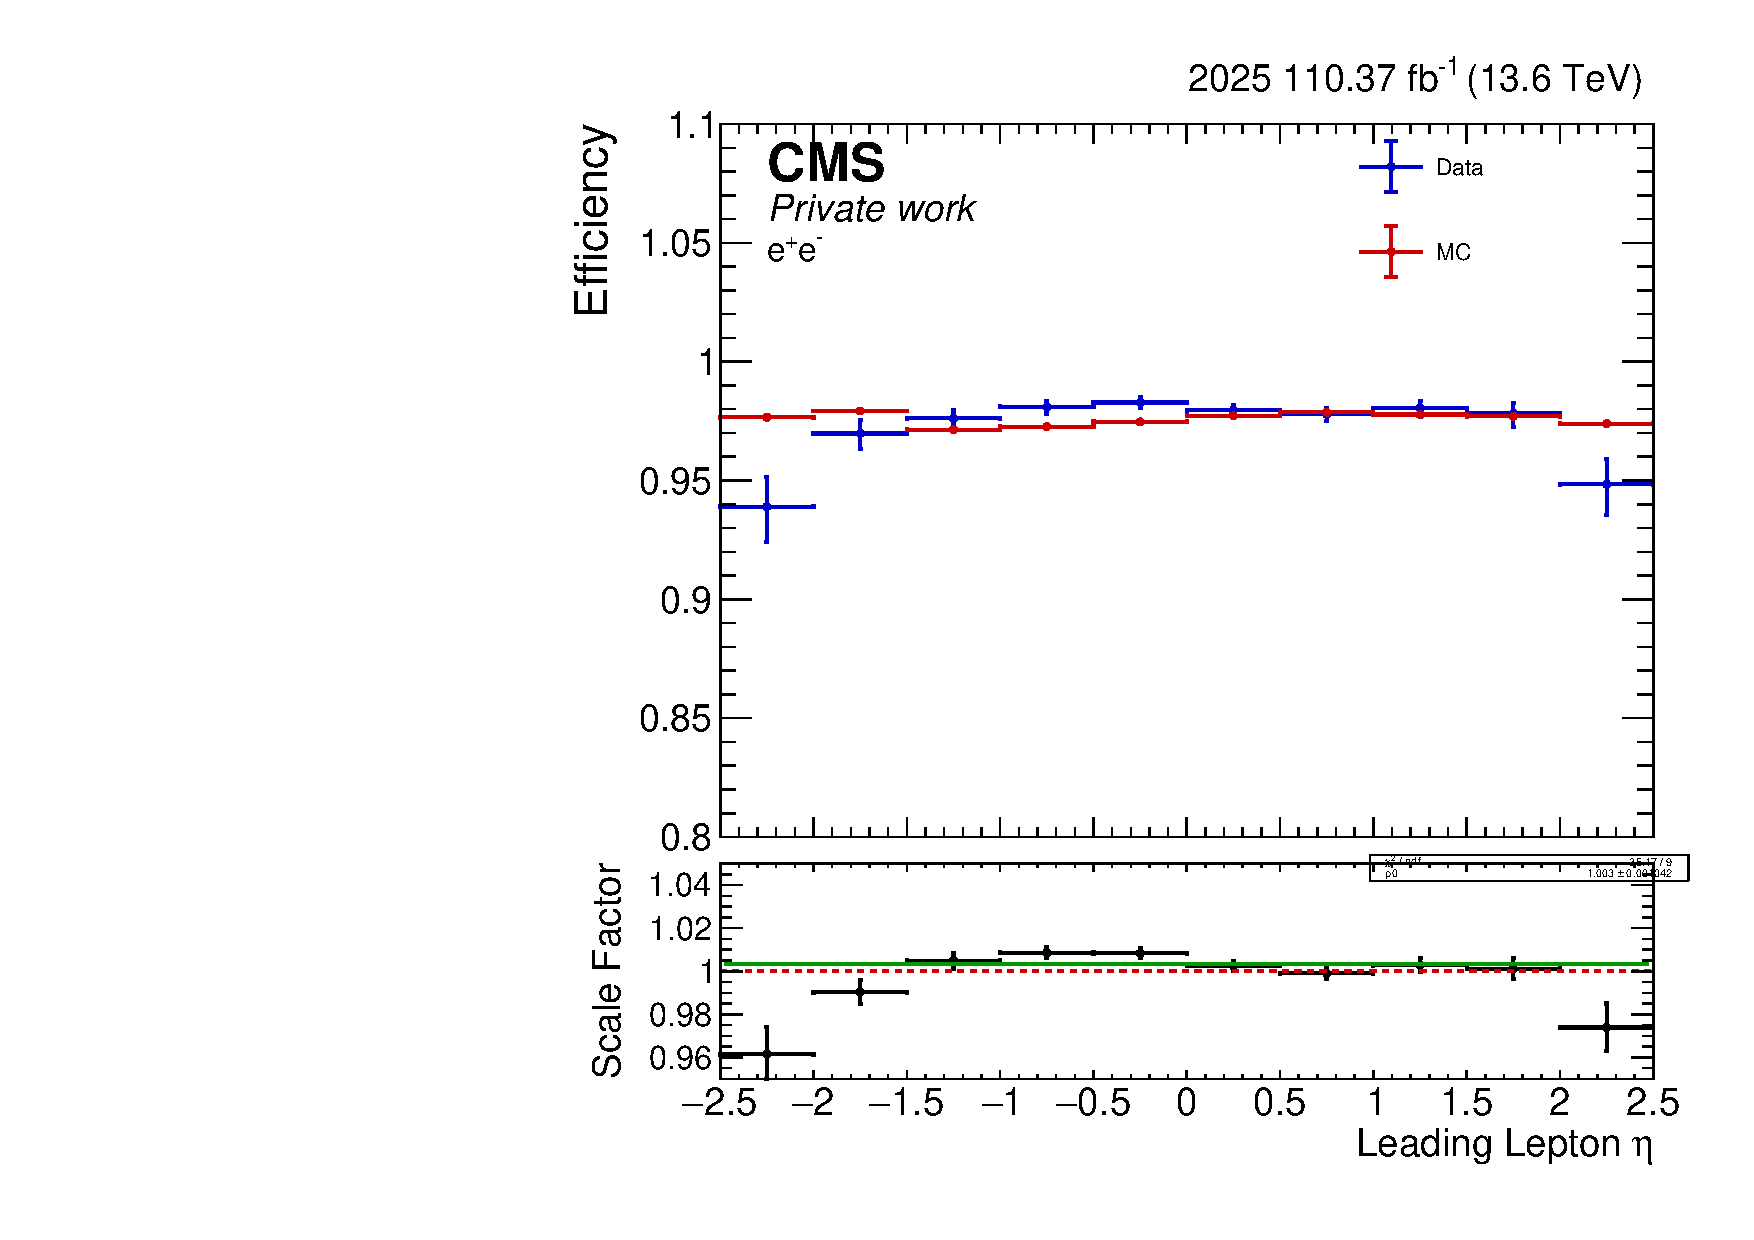
\includegraphics[width=0.48\linewidth]{figures/2025/ElEl/ScaleFactor/SF_Lep1eta.pdf}
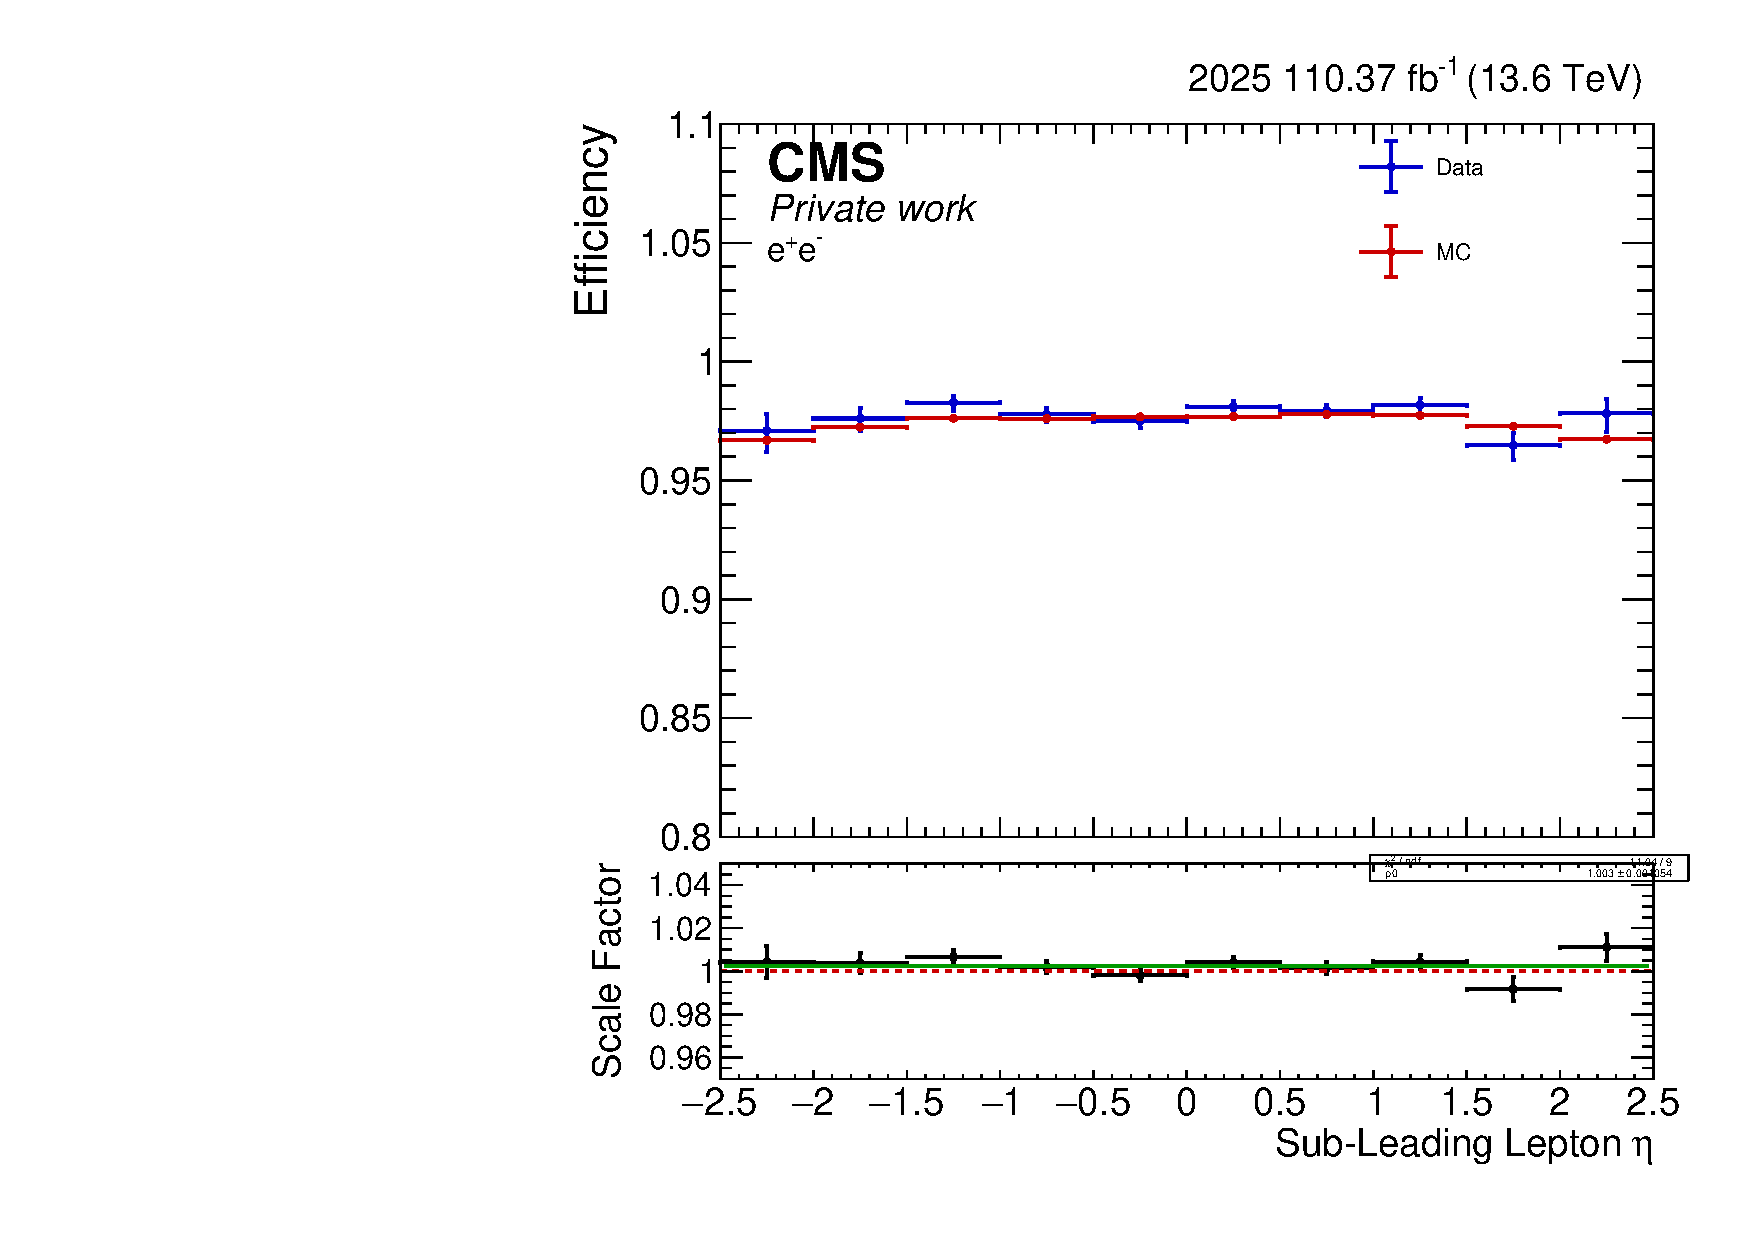
\includegraphics[width=0.48\linewidth]{figures/2025/ElEl/ScaleFactor/SF_Lep2eta.pdf}
\caption{Additional one-dimensional efficiency and SF diagnostics in the $ee$ channel. Variables and binning are shown on each axis.}\label{fig:diag-ElEl-SF_Lep1eta-2025}
\end{figure}
\begin{figure}[htbp]\centering
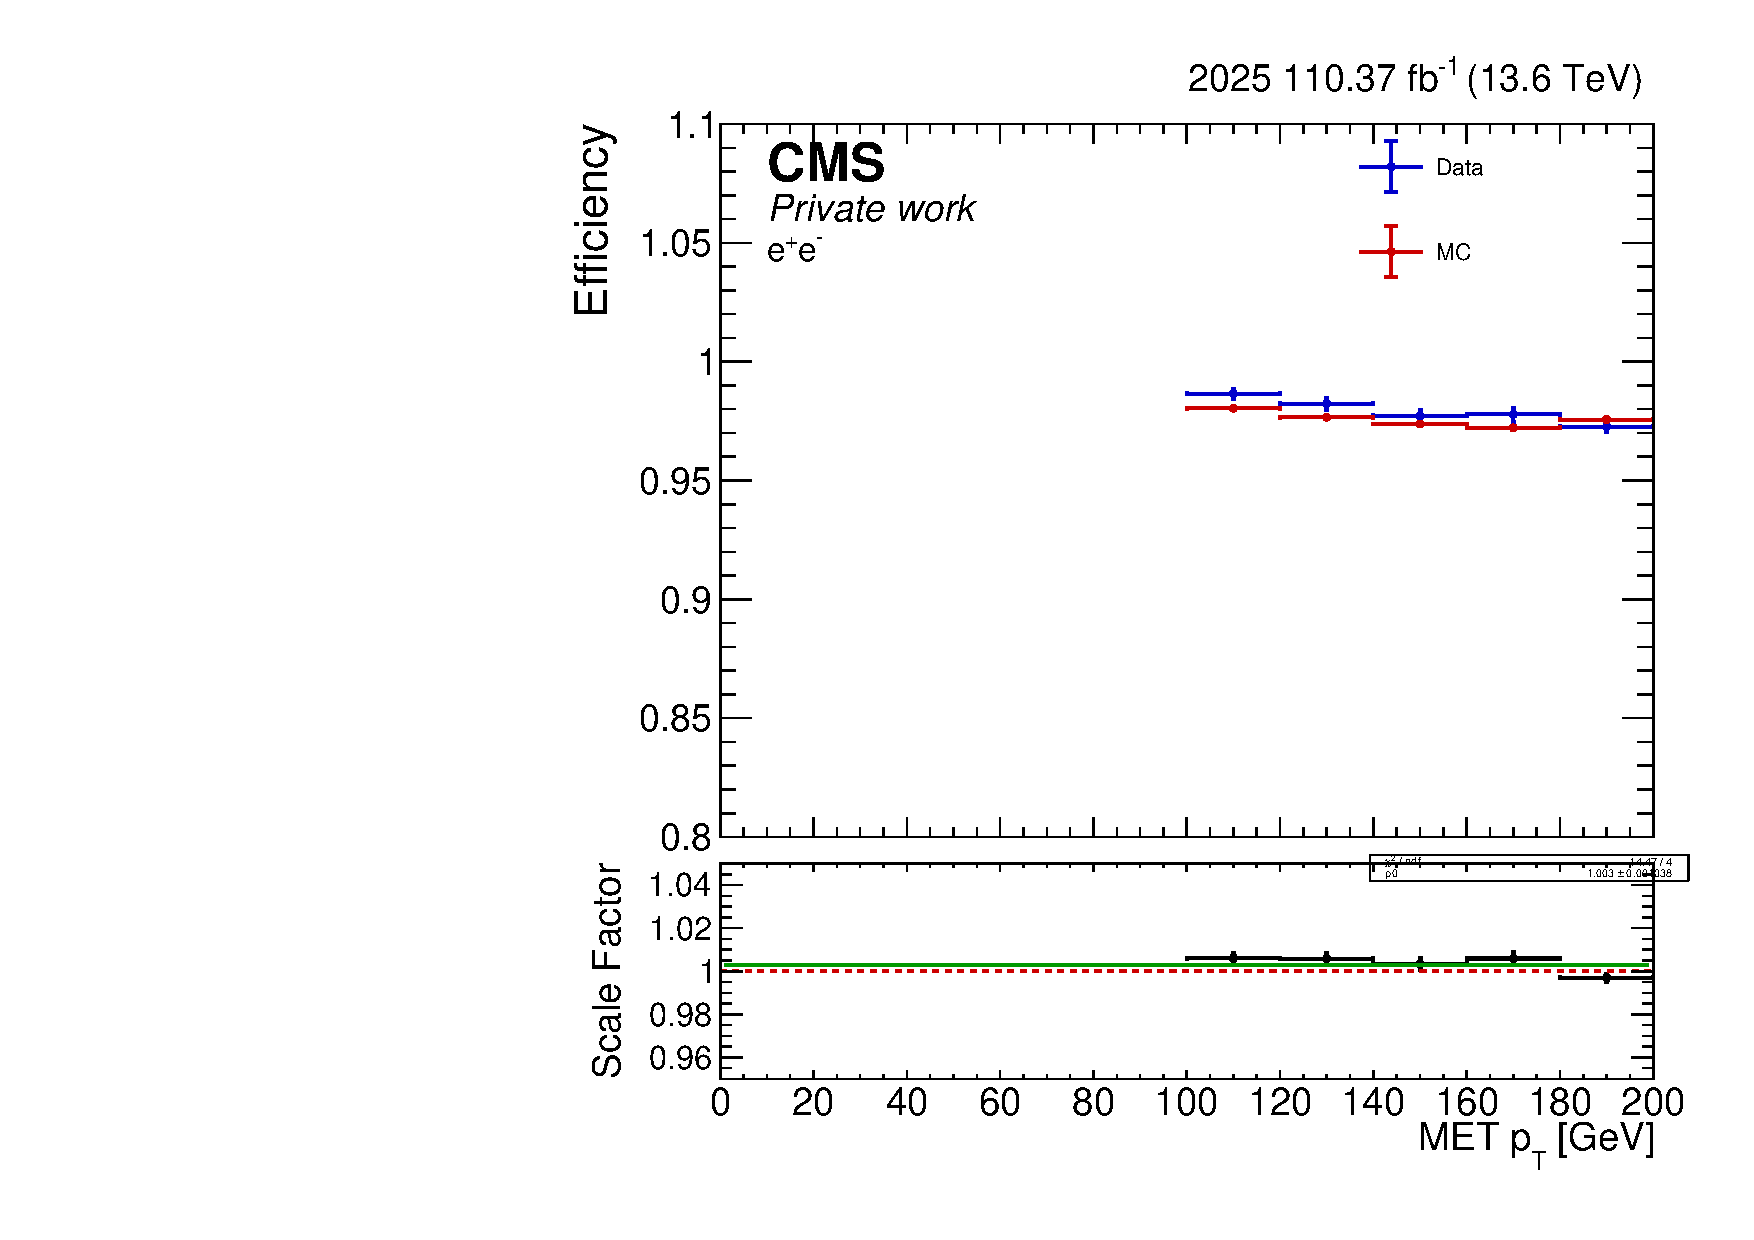
\includegraphics[width=0.48\linewidth]{figures/2025/ElEl/ScaleFactor/SF_METpt.pdf}
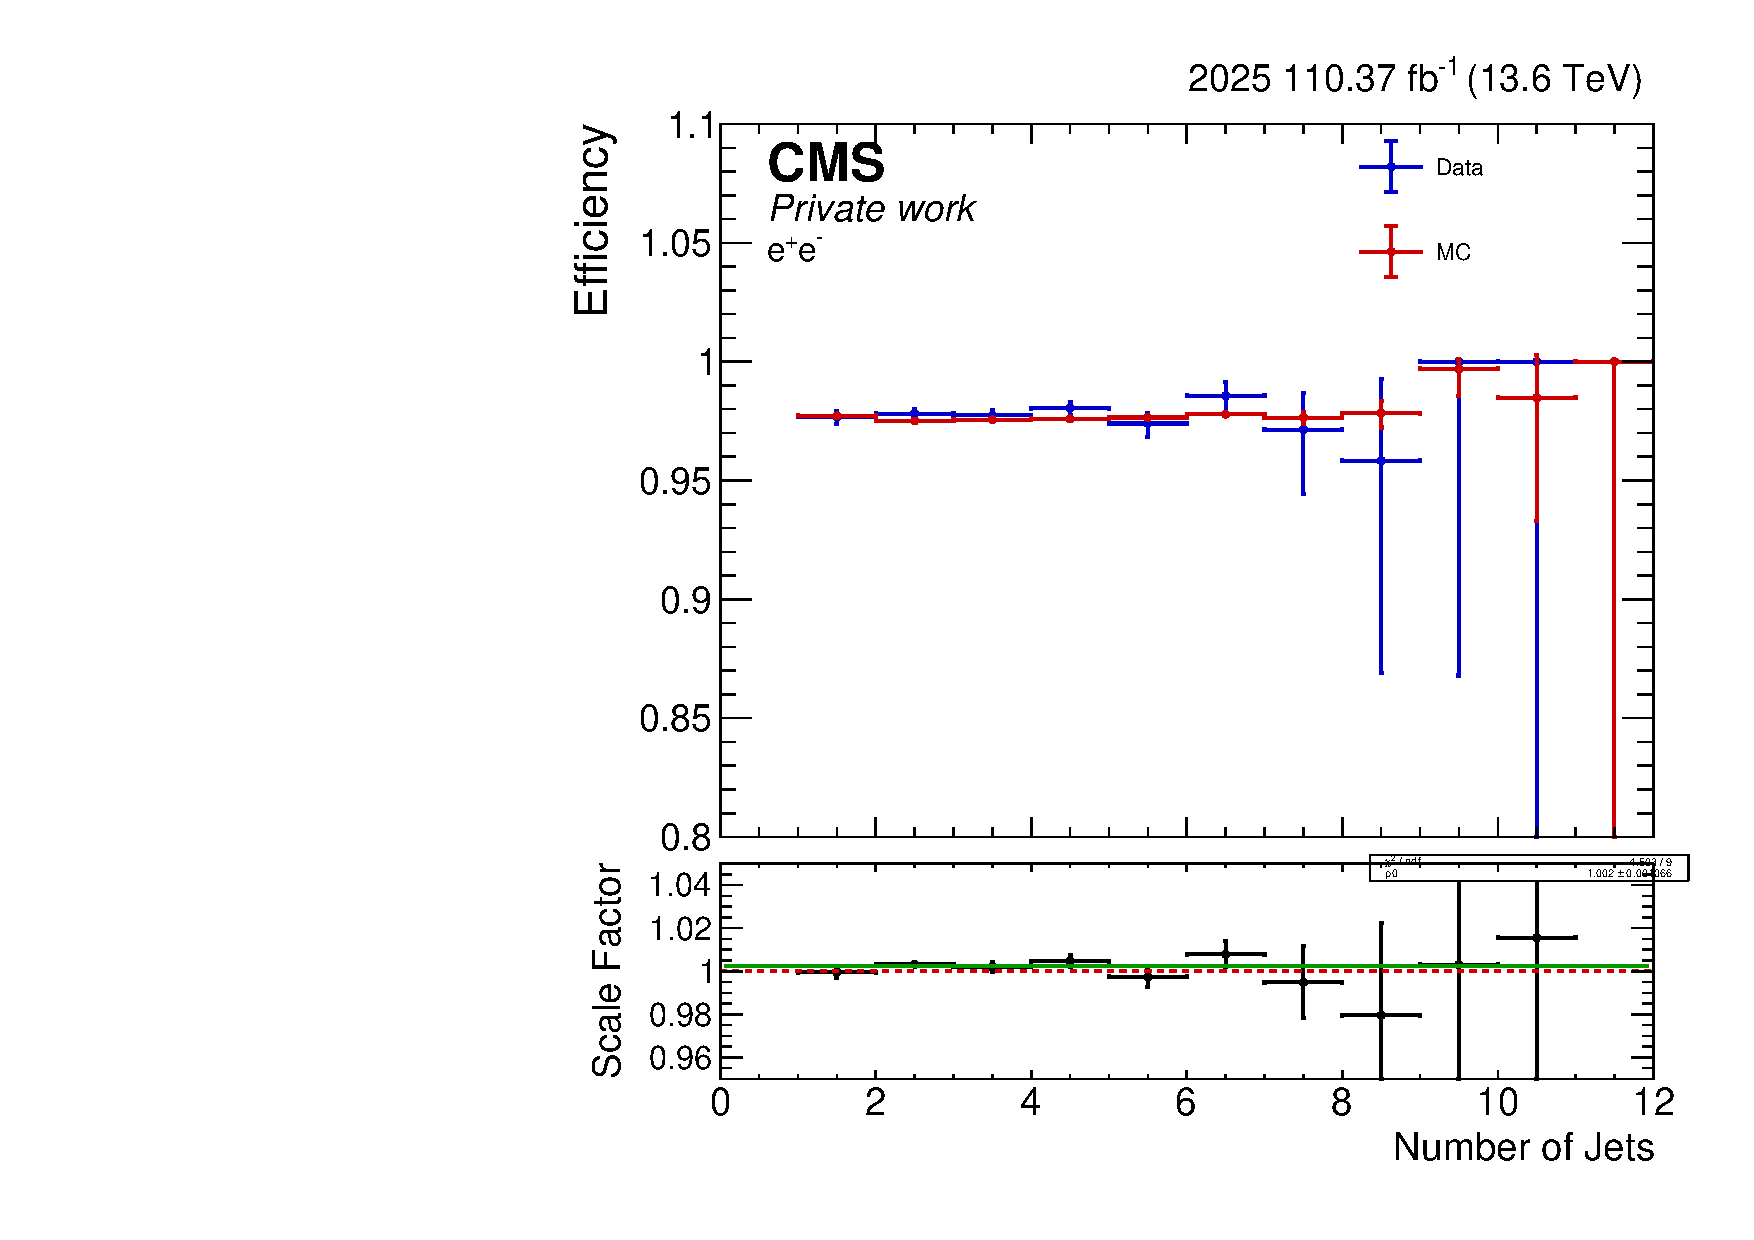
\includegraphics[width=0.48\linewidth]{figures/2025/ElEl/ScaleFactor/SF_Num_Jets.pdf}
\caption{Additional one-dimensional efficiency and SF diagnostics in the $ee$ channel. Variables and binning are shown on each axis.}\label{fig:diag-ElEl-SF_METpt-2025}
\end{figure}
\begin{figure}[htbp]\centering
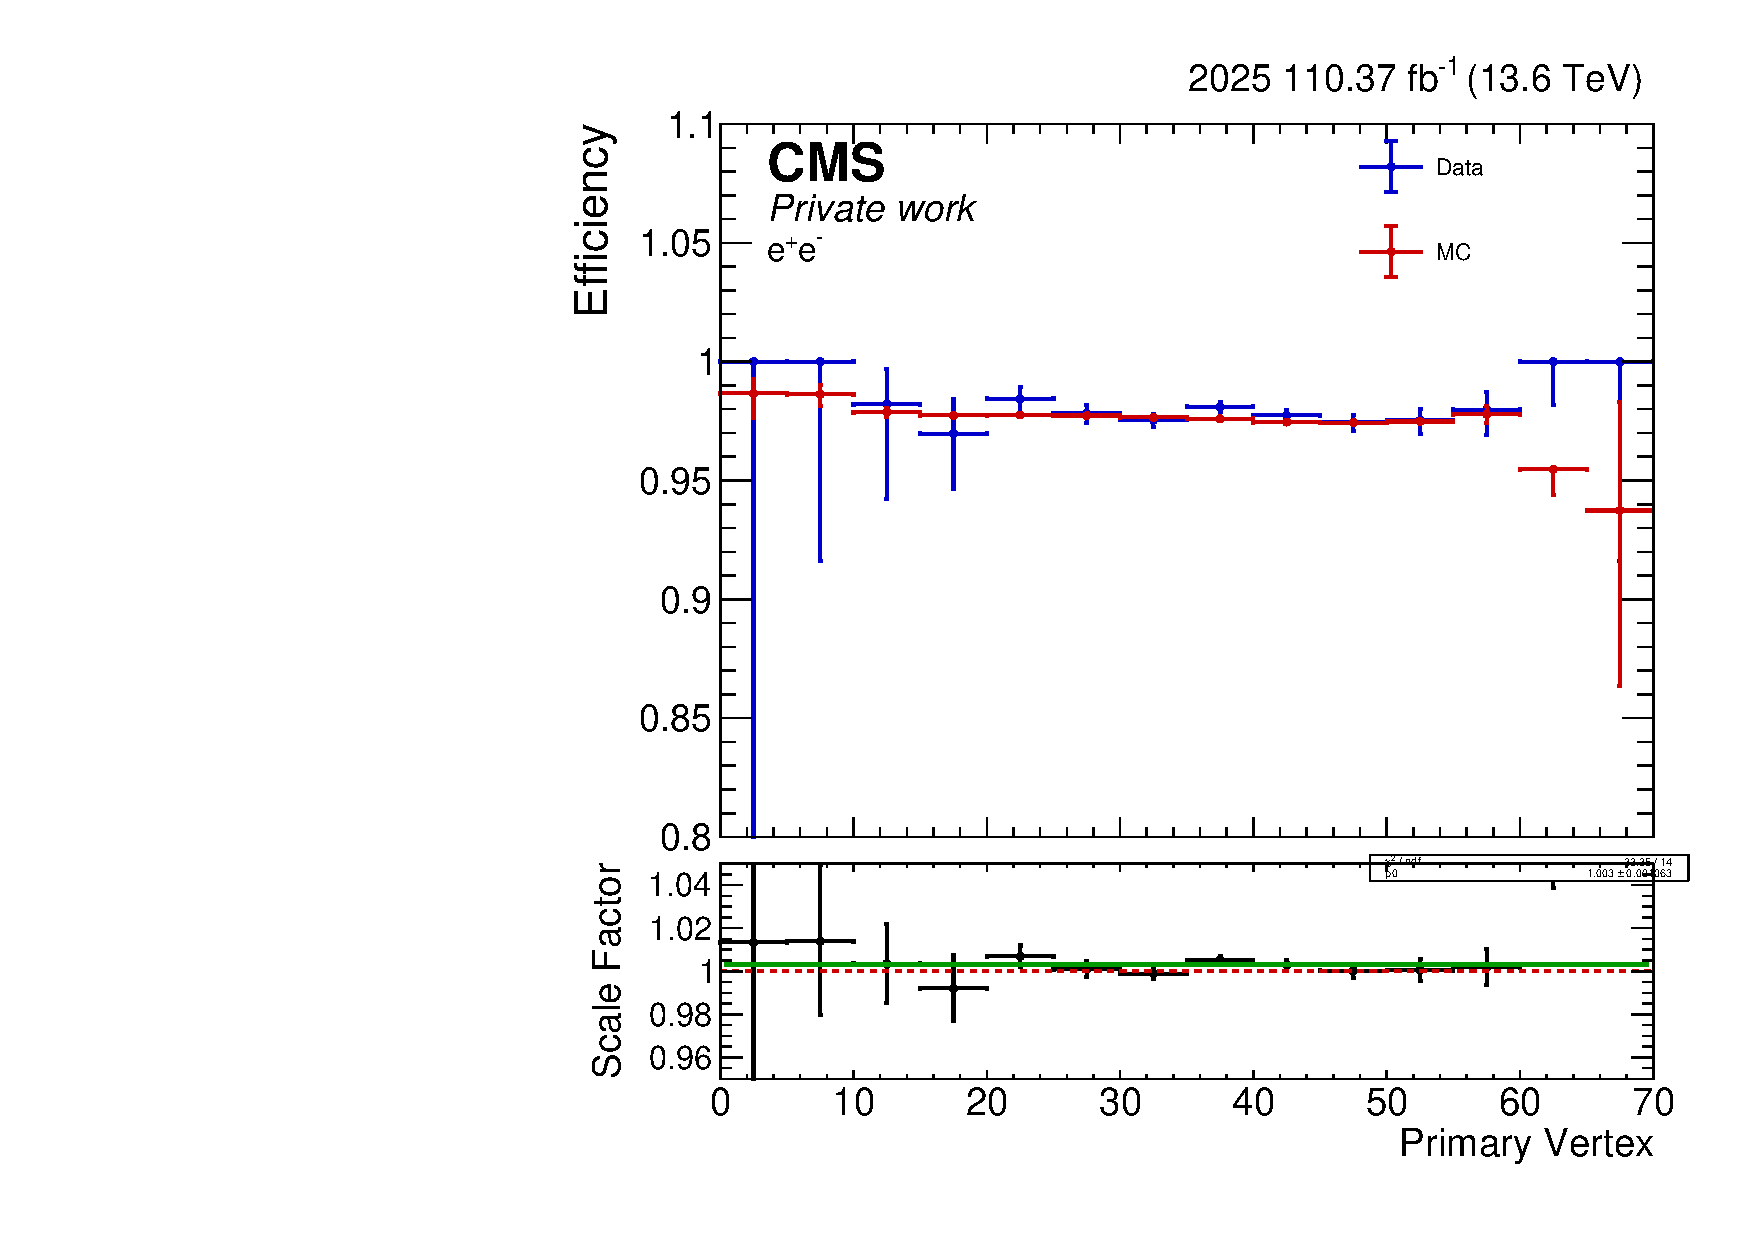
\includegraphics[width=0.48\linewidth]{figures/2025/ElEl/ScaleFactor/SF_Num_PV.pdf}
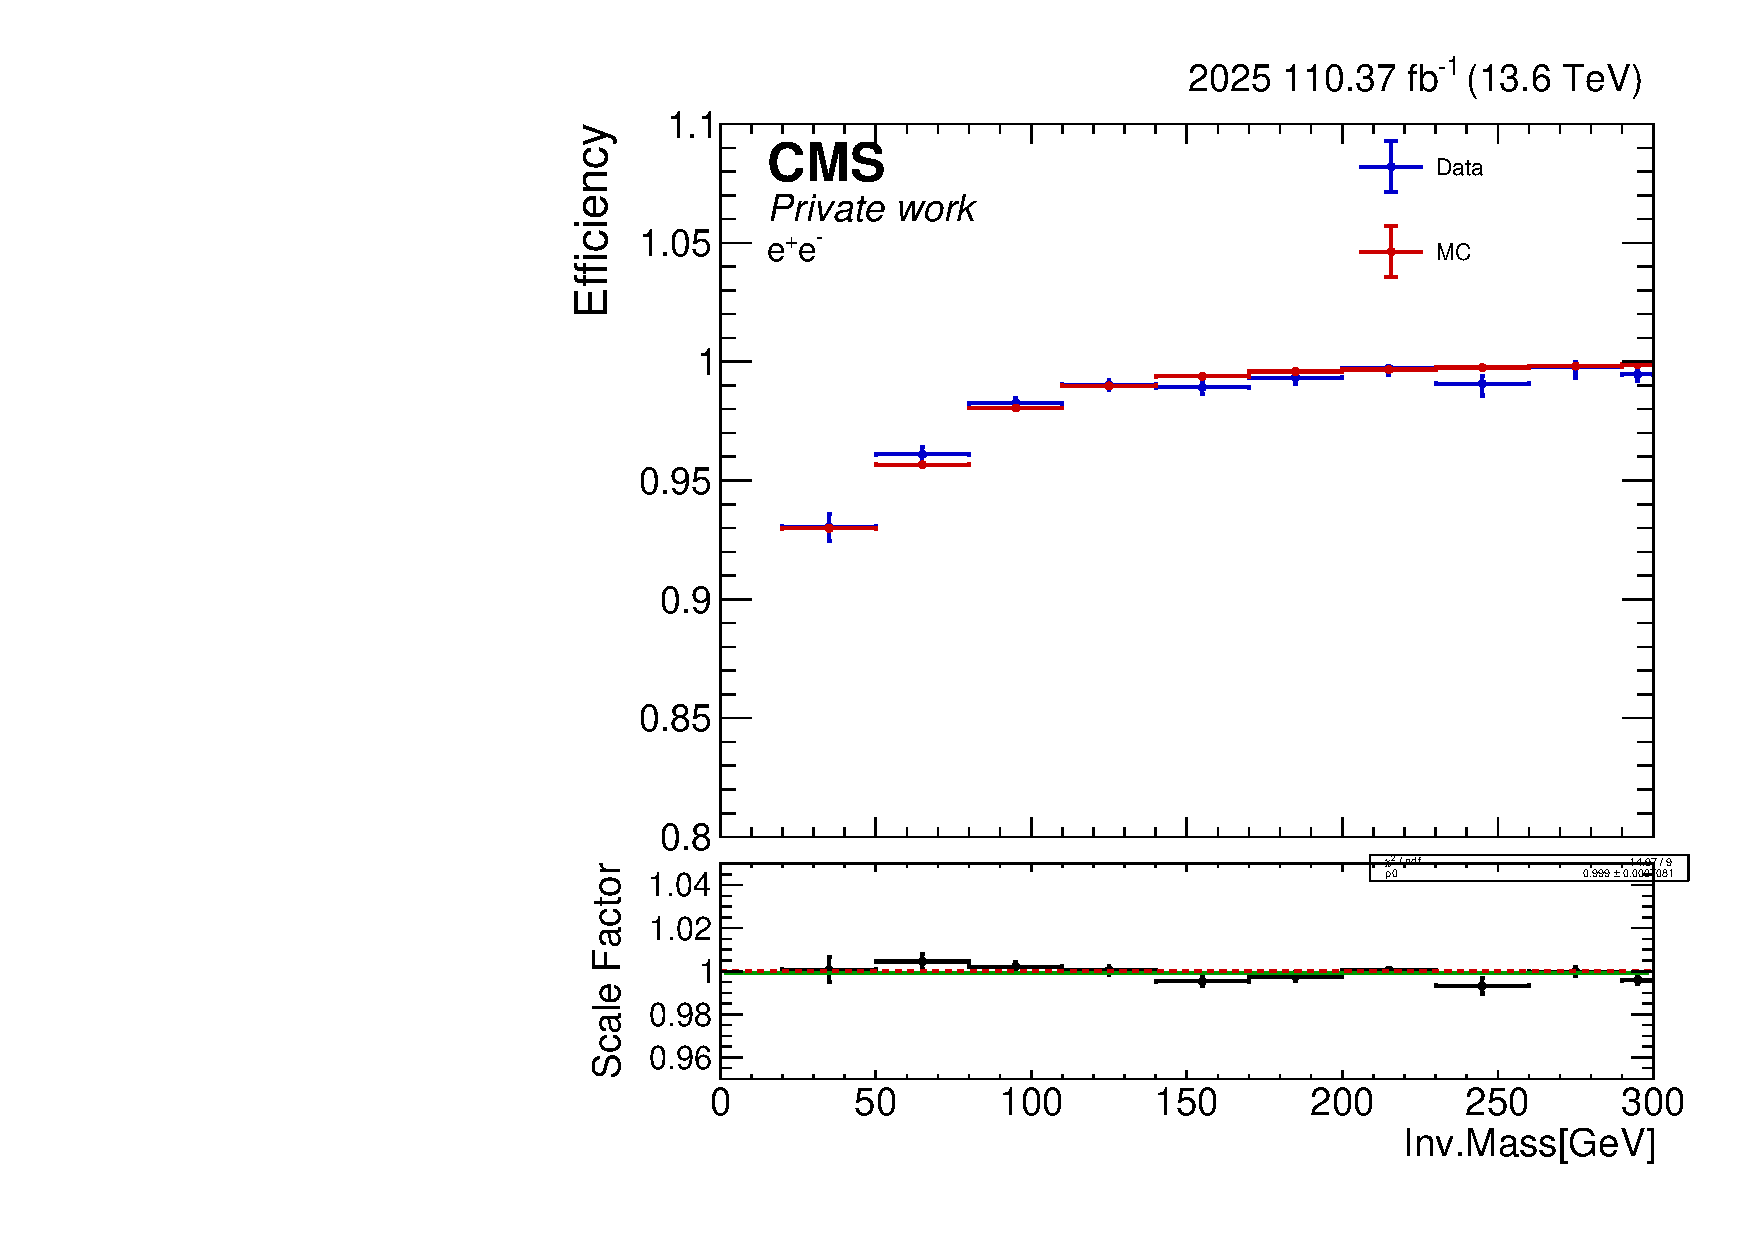
\includegraphics[width=0.48\linewidth]{figures/2025/ElEl/ScaleFactor/SF_DiLepMass.pdf}
\caption{Additional one-dimensional efficiency and SF diagnostics in the $ee$ channel. Variables and binning are shown on each axis.}\label{fig:diag-ElEl-SF_Num_PV-2025}
\end{figure}
\begin{figure}[htbp]\centering
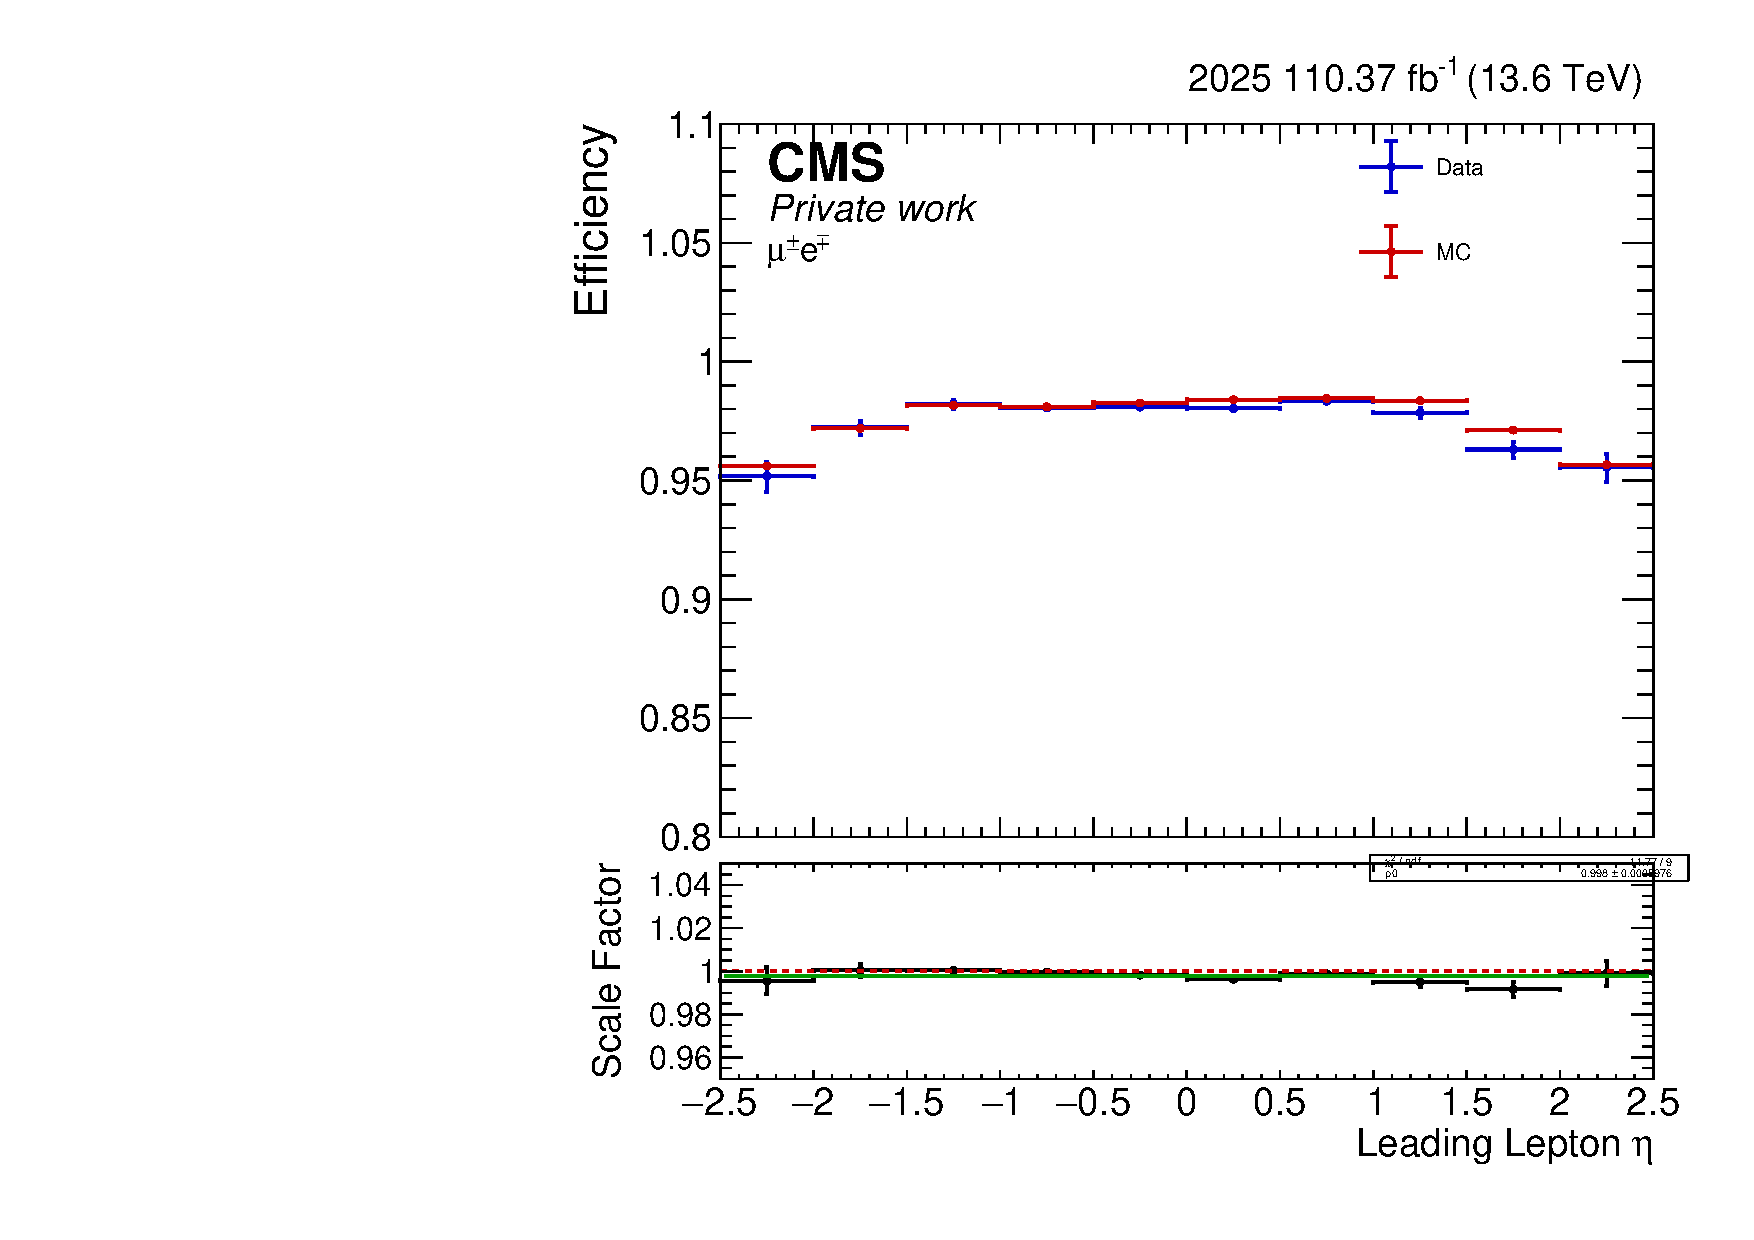
\includegraphics[width=0.48\linewidth]{figures/2025/MuEl/ScaleFactor/SF_Lep1eta.pdf}
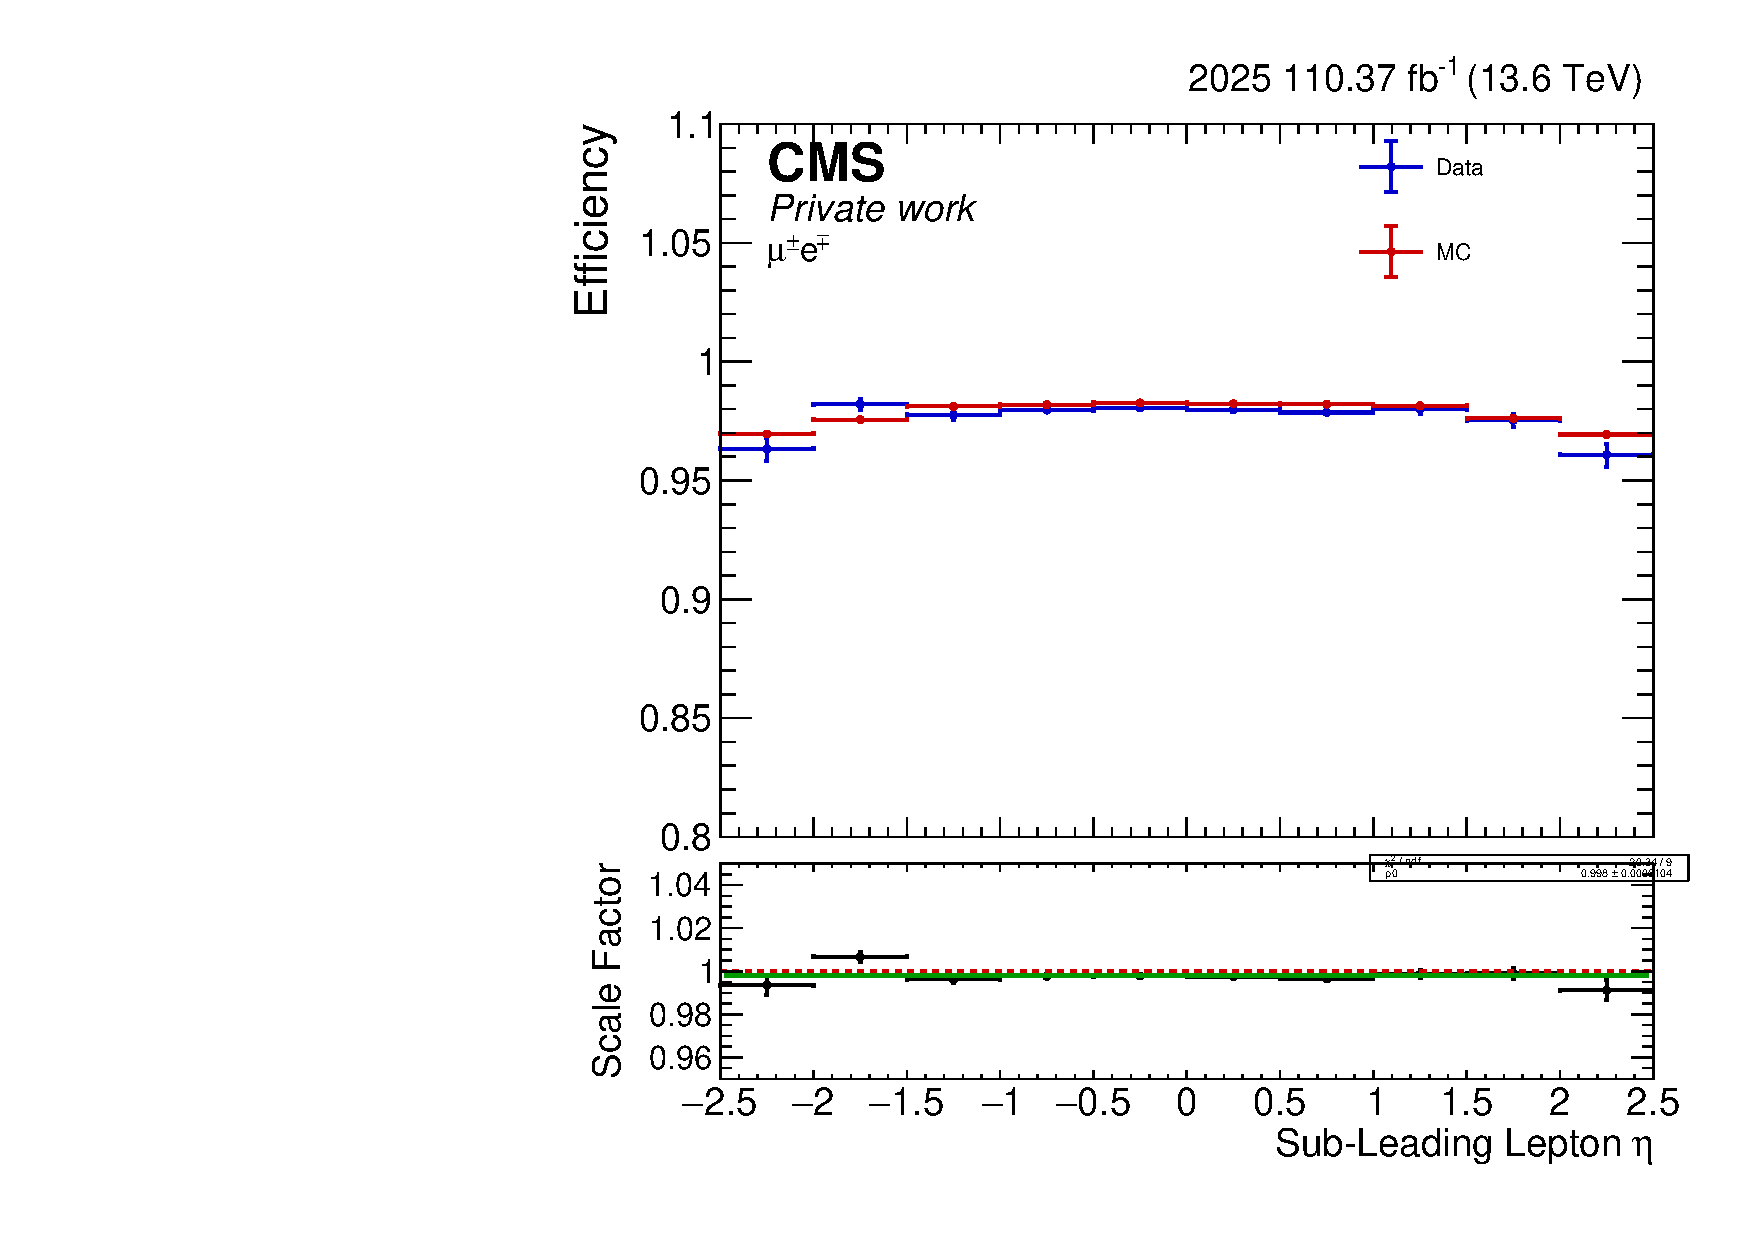
\includegraphics[width=0.48\linewidth]{figures/2025/MuEl/ScaleFactor/SF_Lep2eta.pdf}
\caption{Additional one-dimensional efficiency and SF diagnostics in the $e\mu$ channel. Variables and binning are shown on each axis.}\label{fig:diag-MuEl-SF_Lep1eta-2025}
\end{figure}
\begin{figure}[htbp]\centering
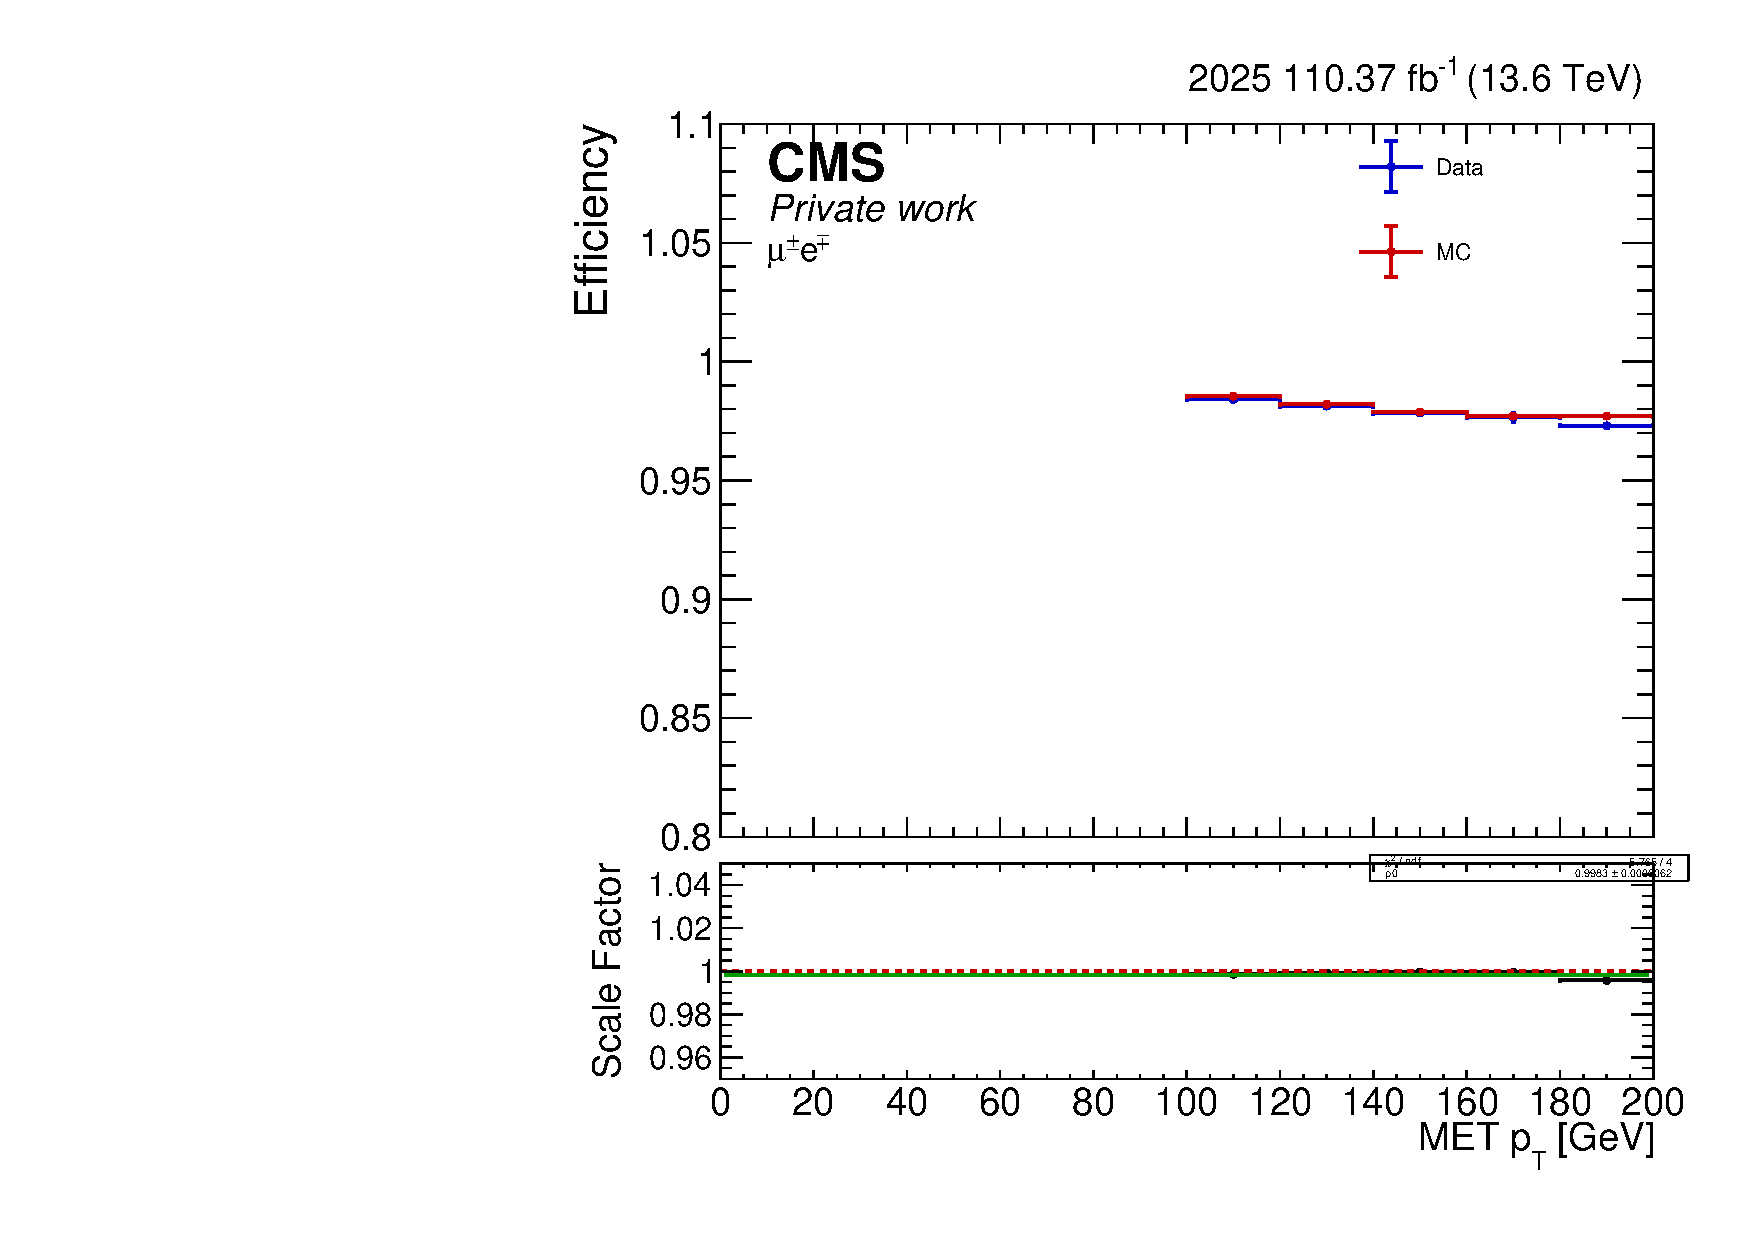
\includegraphics[width=0.48\linewidth]{figures/2025/MuEl/ScaleFactor/SF_METpt.pdf}
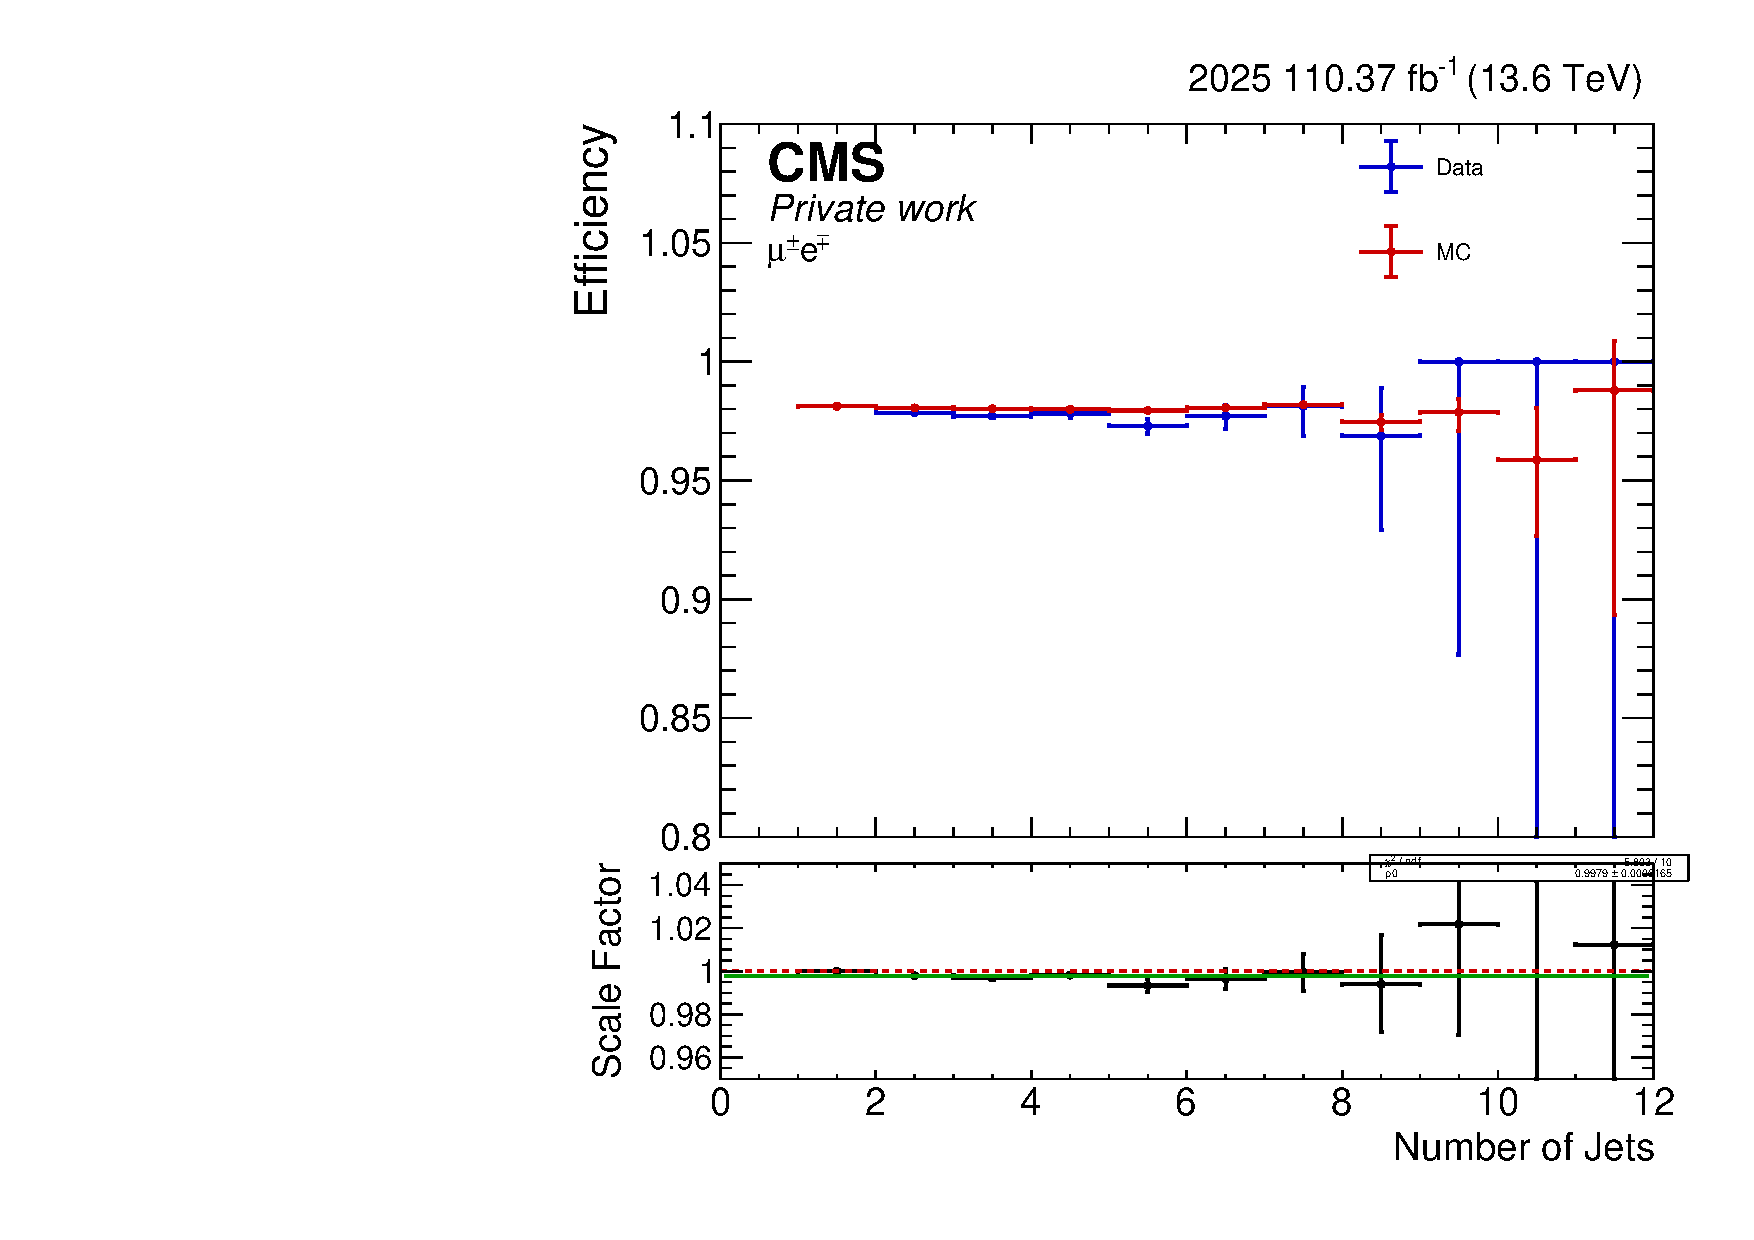
\includegraphics[width=0.48\linewidth]{figures/2025/MuEl/ScaleFactor/SF_Num_Jets.pdf}
\caption{Additional one-dimensional efficiency and SF diagnostics in the $e\mu$ channel. Variables and binning are shown on each axis.}\label{fig:diag-MuEl-SF_METpt-2025}
\end{figure}
\begin{figure}[htbp]\centering
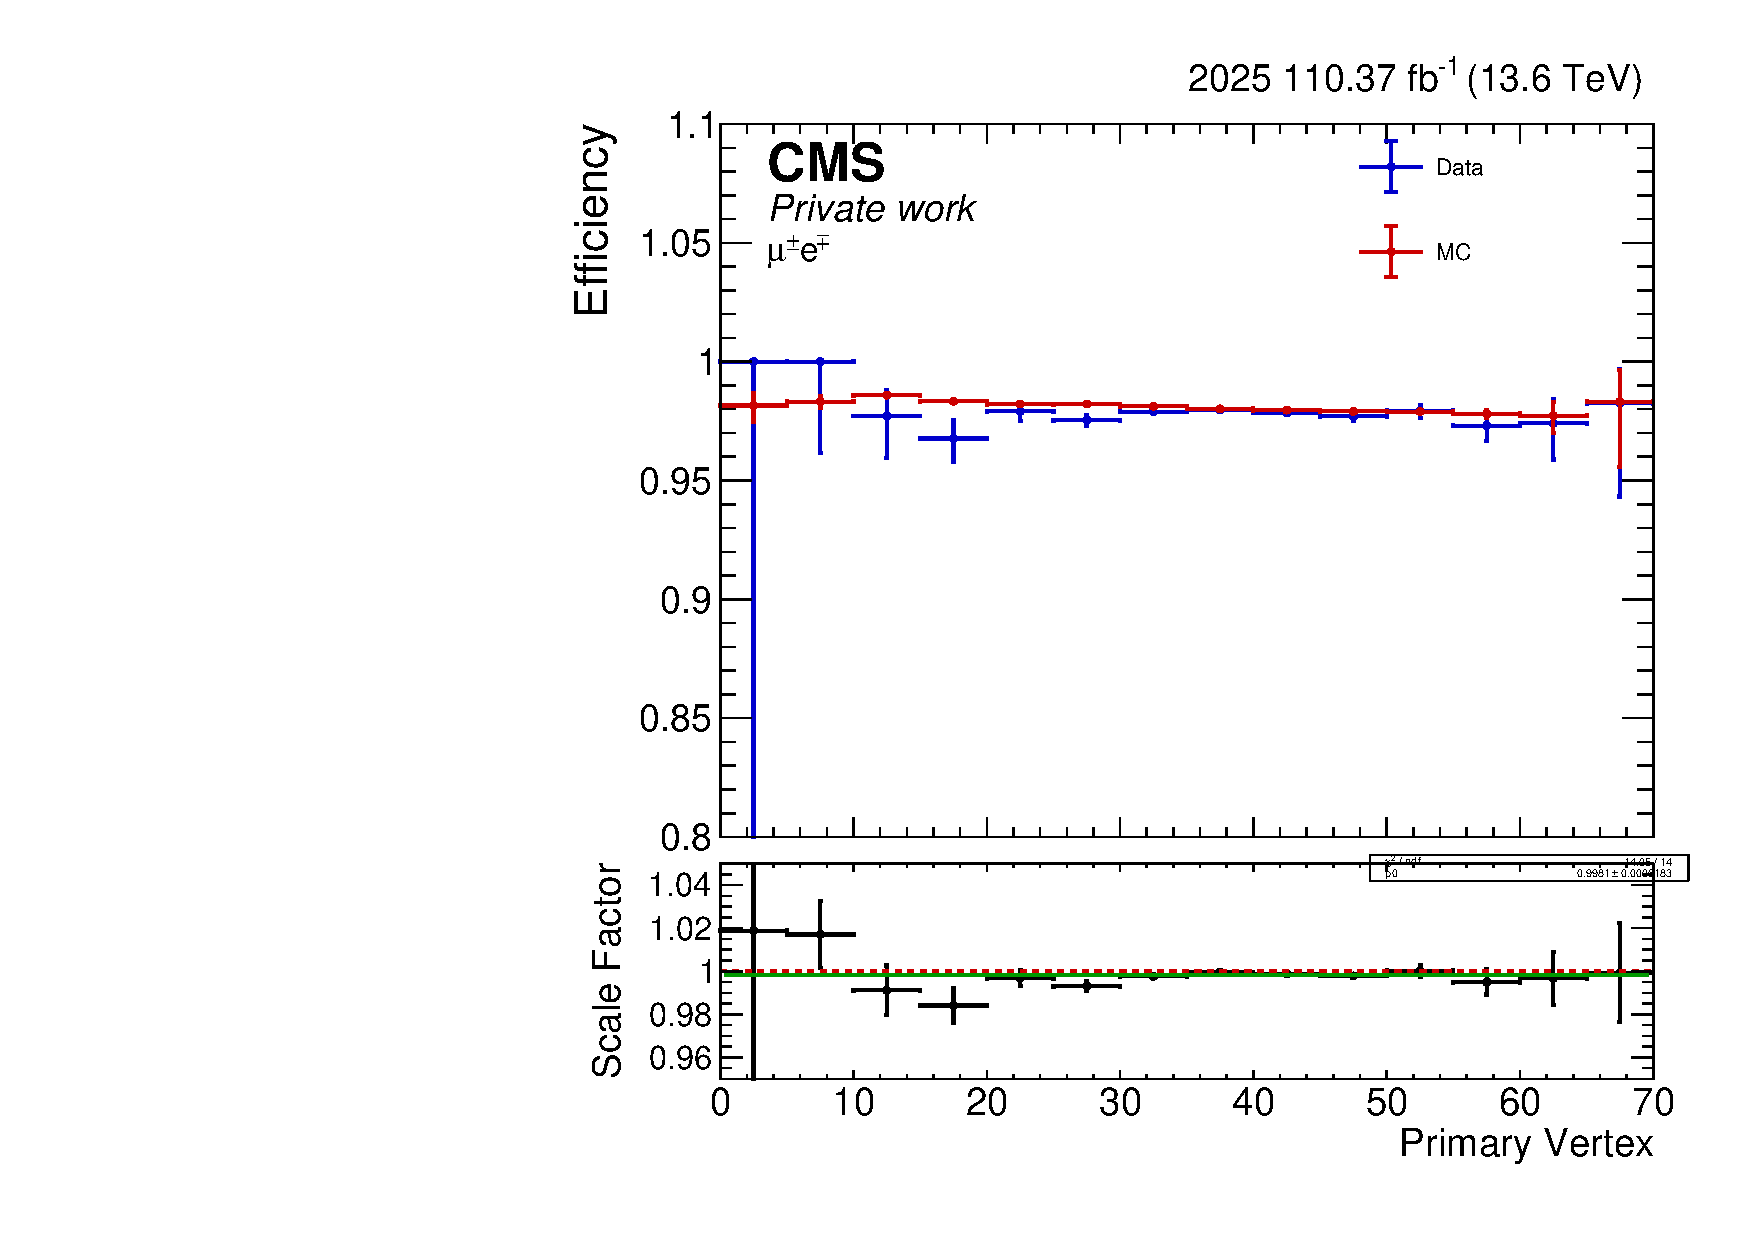
\includegraphics[width=0.48\linewidth]{figures/2025/MuEl/ScaleFactor/SF_Num_PV.pdf}
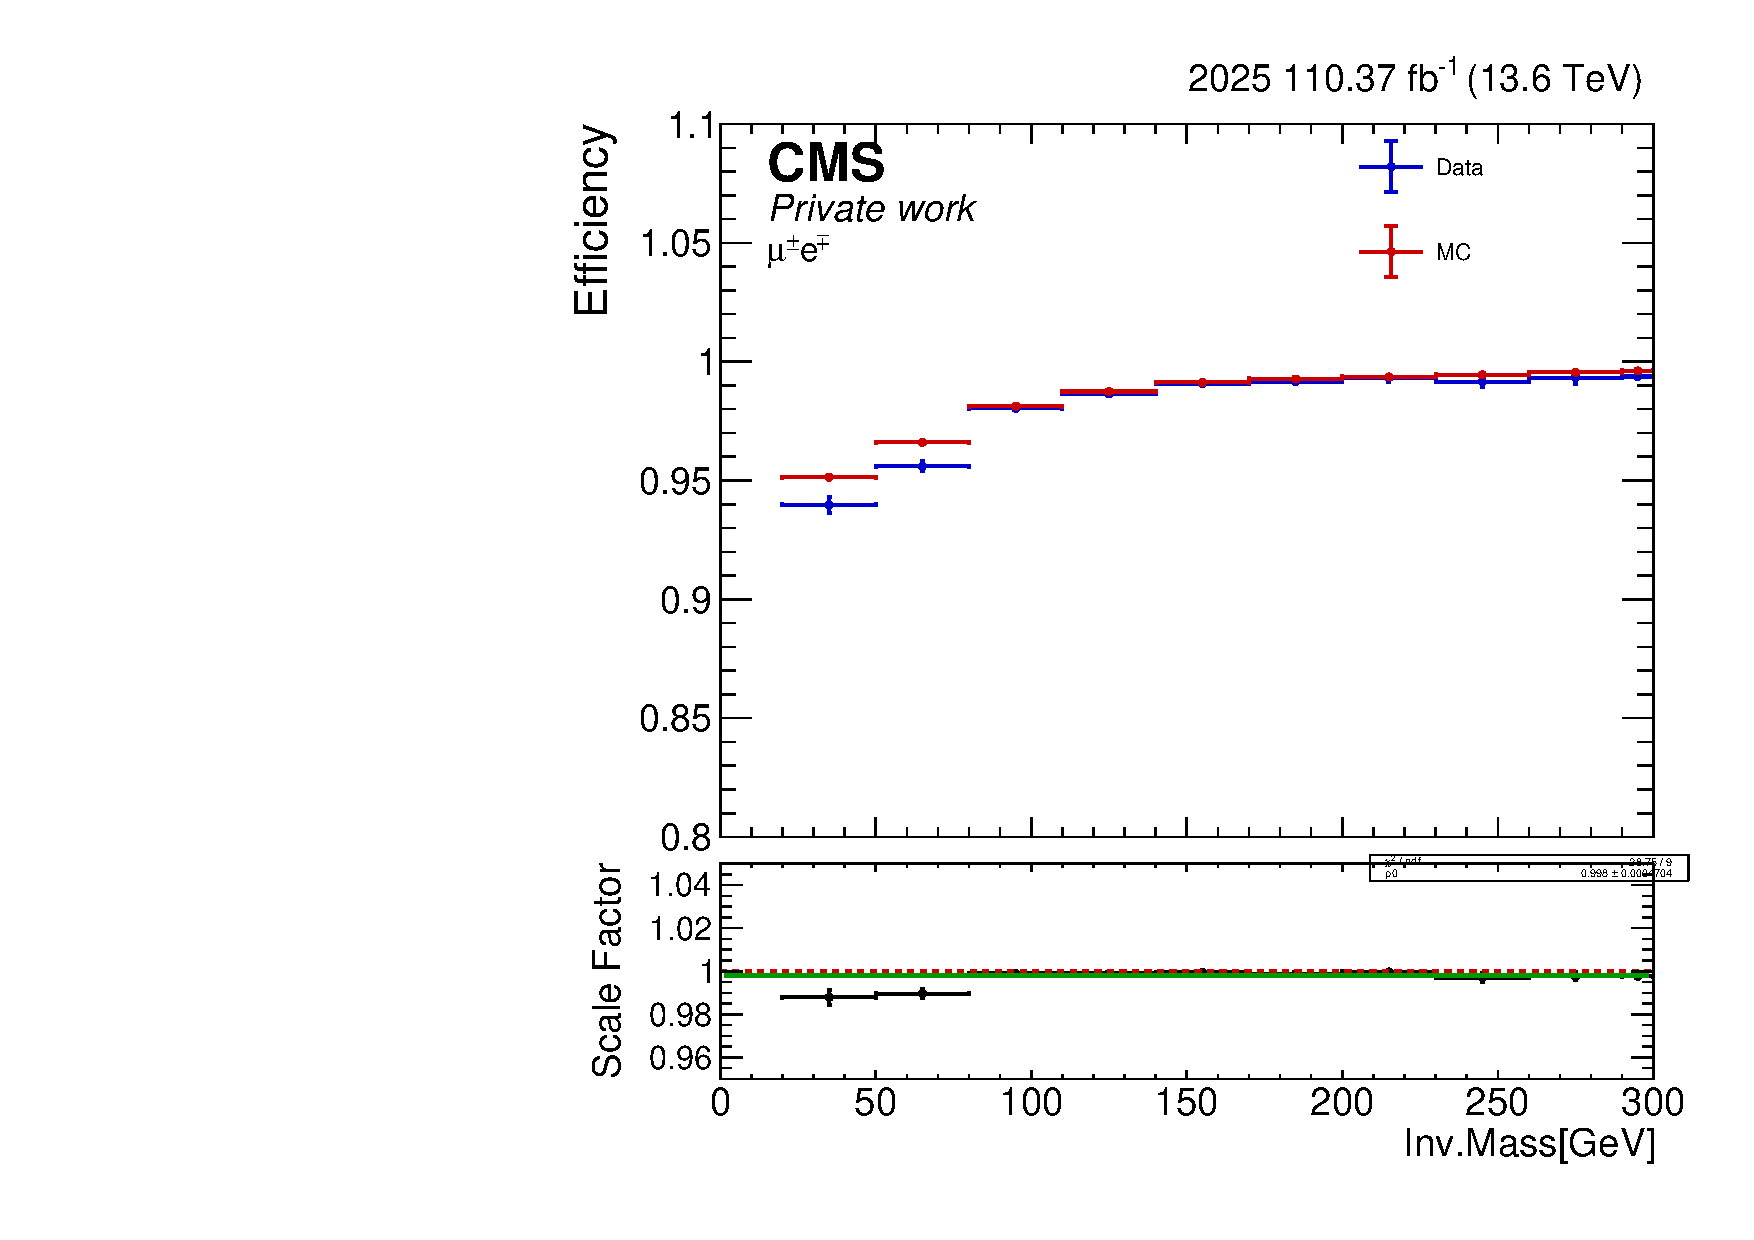
\includegraphics[width=0.48\linewidth]{figures/2025/MuEl/ScaleFactor/SF_DiLepMass.pdf}
\caption{Additional one-dimensional efficiency and SF diagnostics in the $e\mu$ channel. Variables and binning are shown on each axis.}\label{fig:diag-MuEl-SF_Num_PV-2025}
\end{figure}
\begin{figure}[htbp]\centering
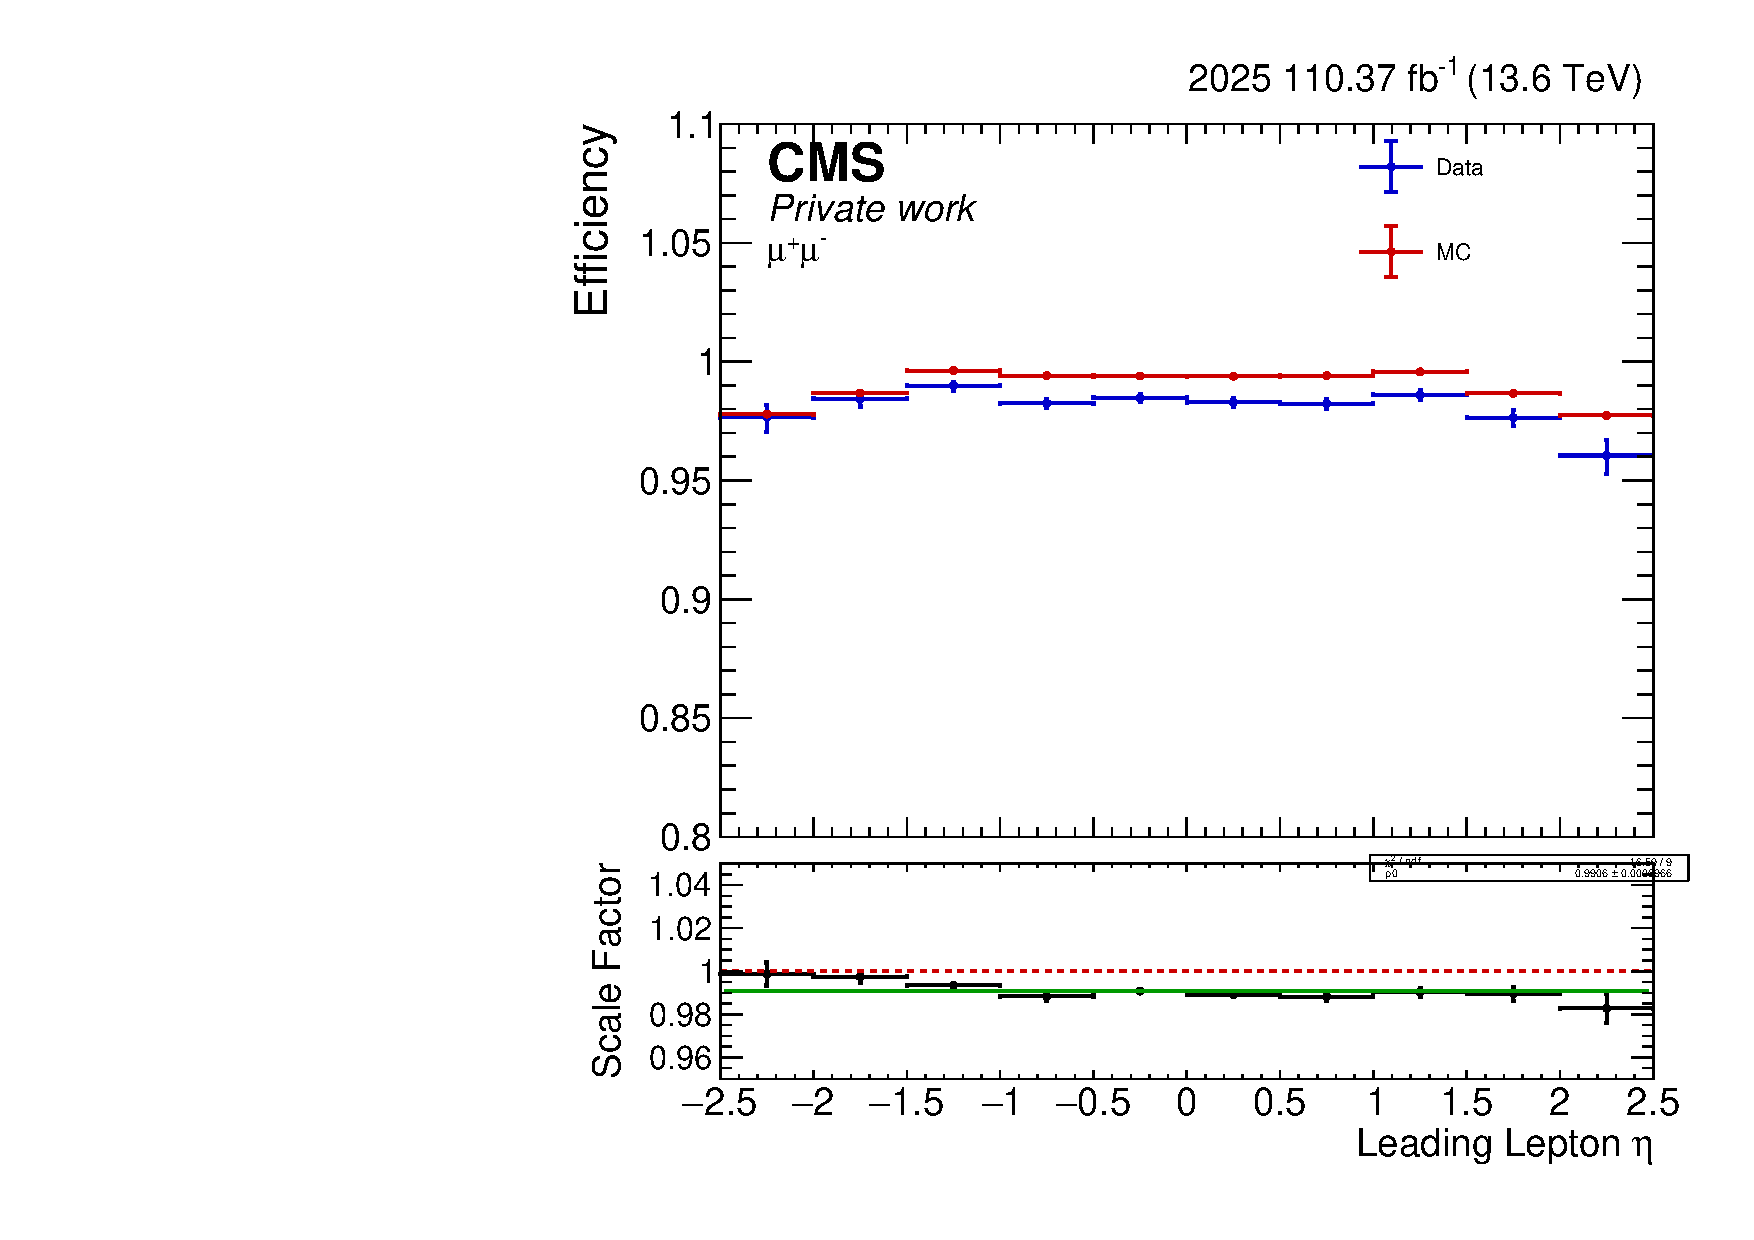
\includegraphics[width=0.48\linewidth]{figures/2025/MuMu/ScaleFactor/SF_Lep1eta.pdf}
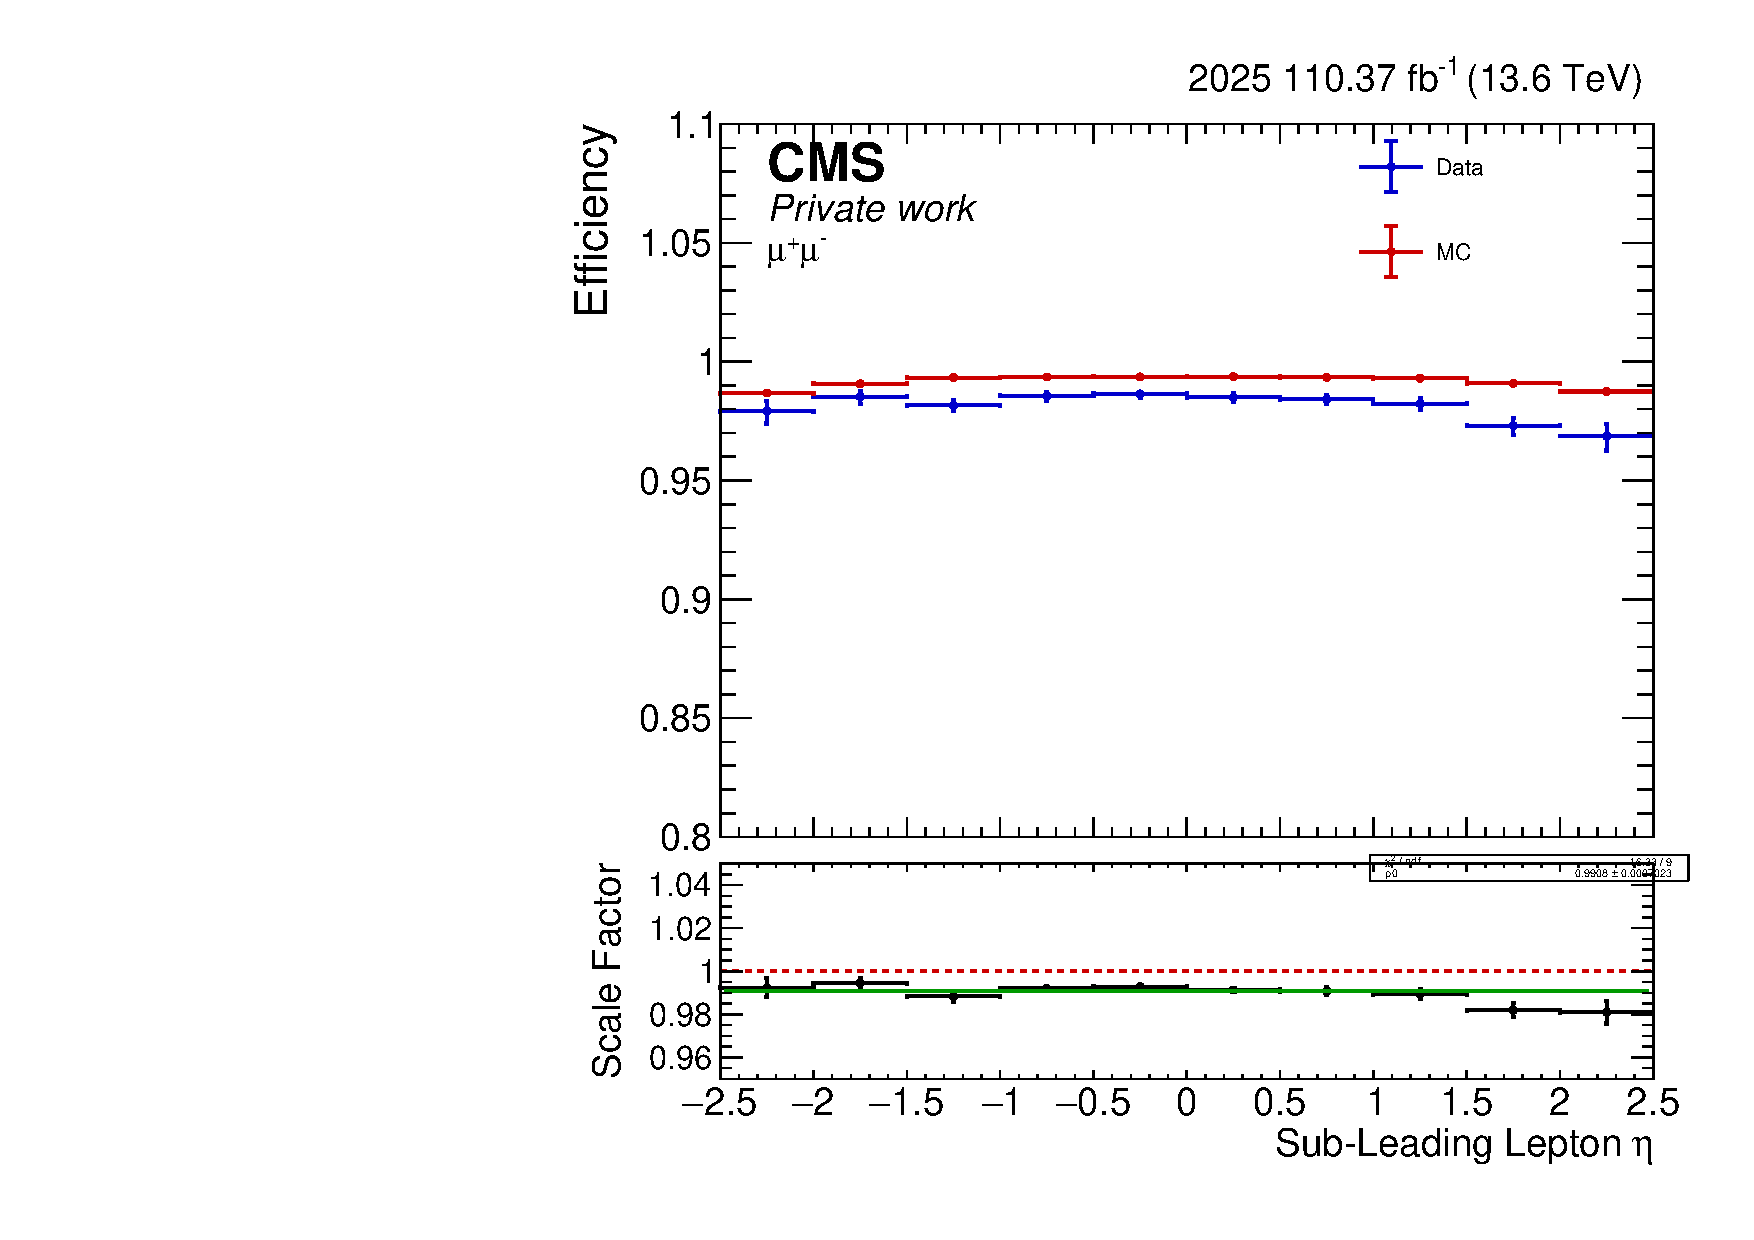
\includegraphics[width=0.48\linewidth]{figures/2025/MuMu/ScaleFactor/SF_Lep2eta.pdf}
\caption{Additional one-dimensional efficiency and SF diagnostics in the $\mu\mu$ channel. Variables and binning are shown on each axis.}\label{fig:diag-MuMu-SF_Lep1eta-2025}
\end{figure}
\begin{figure}[htbp]\centering
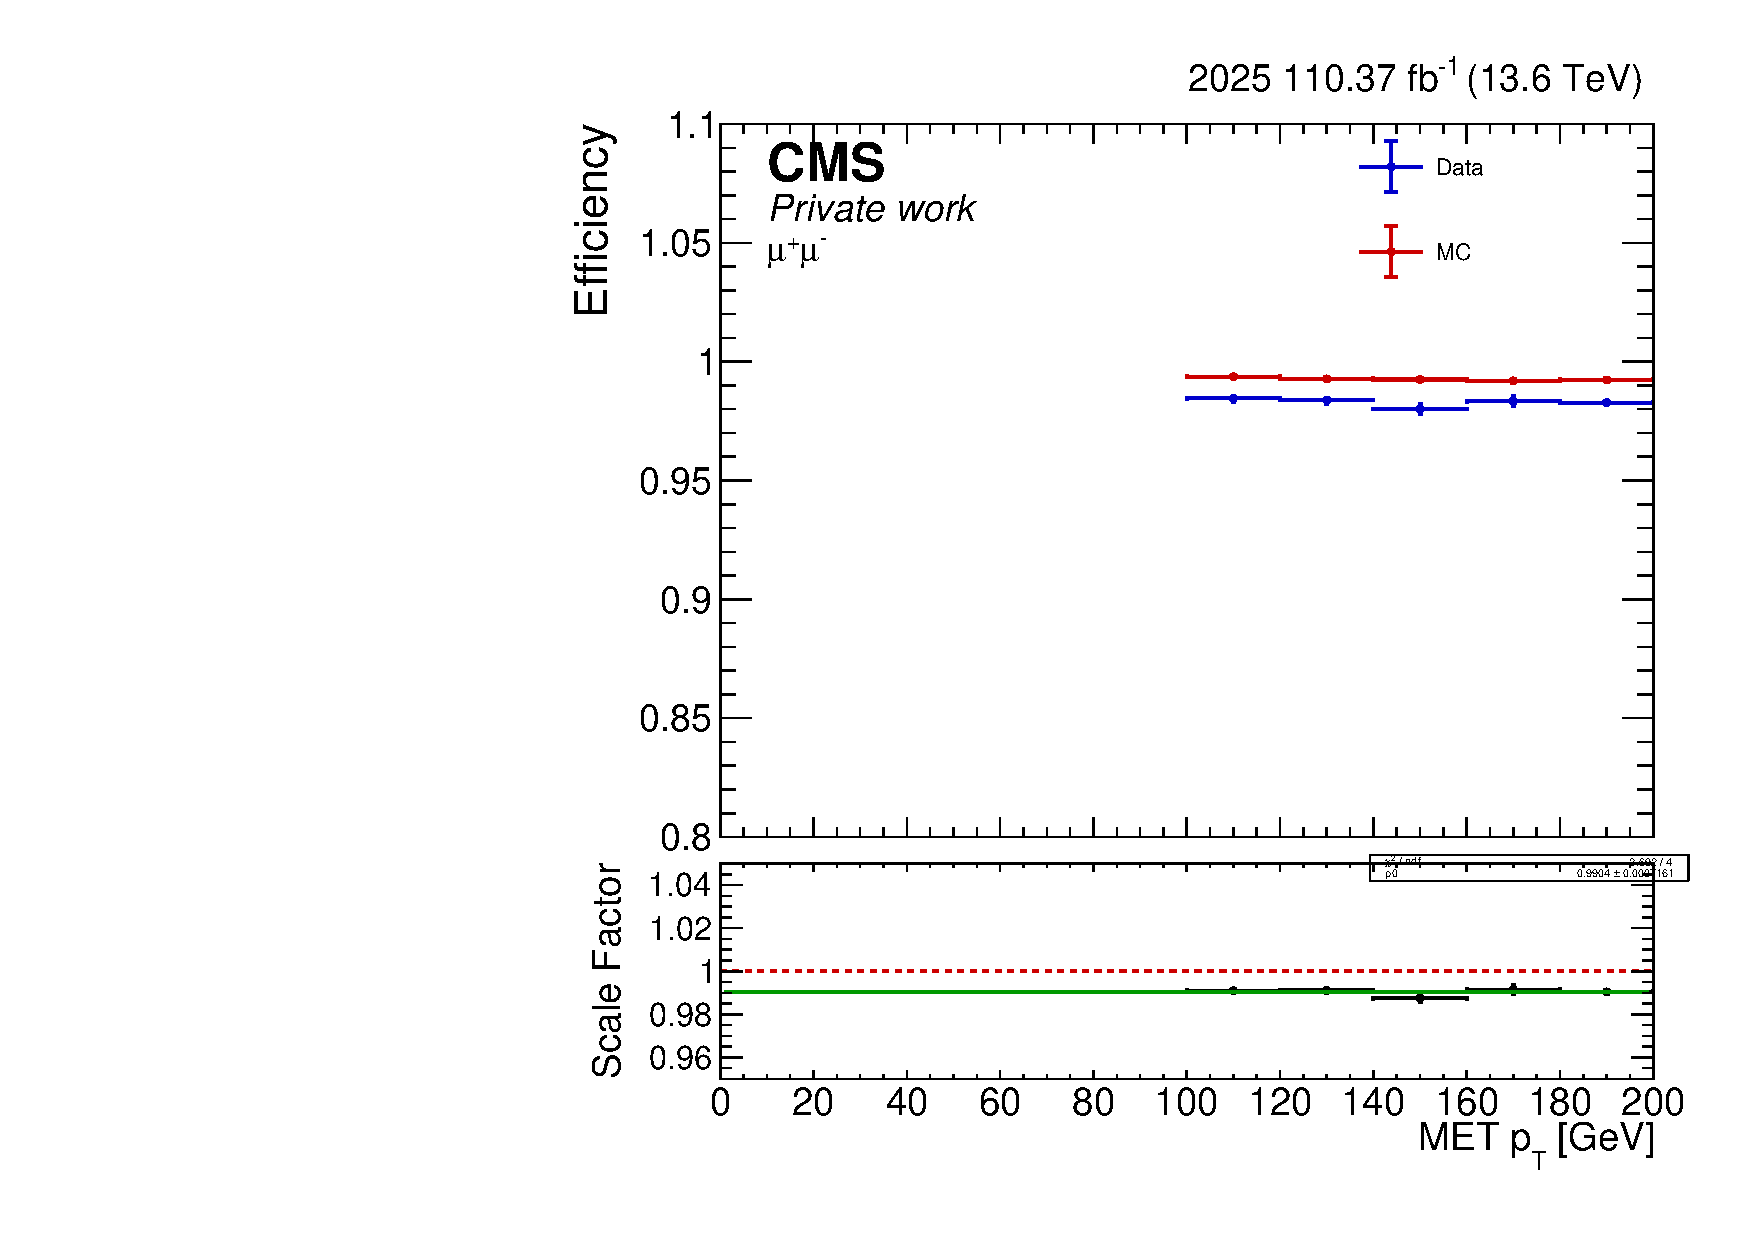
\includegraphics[width=0.48\linewidth]{figures/2025/MuMu/ScaleFactor/SF_METpt.pdf}
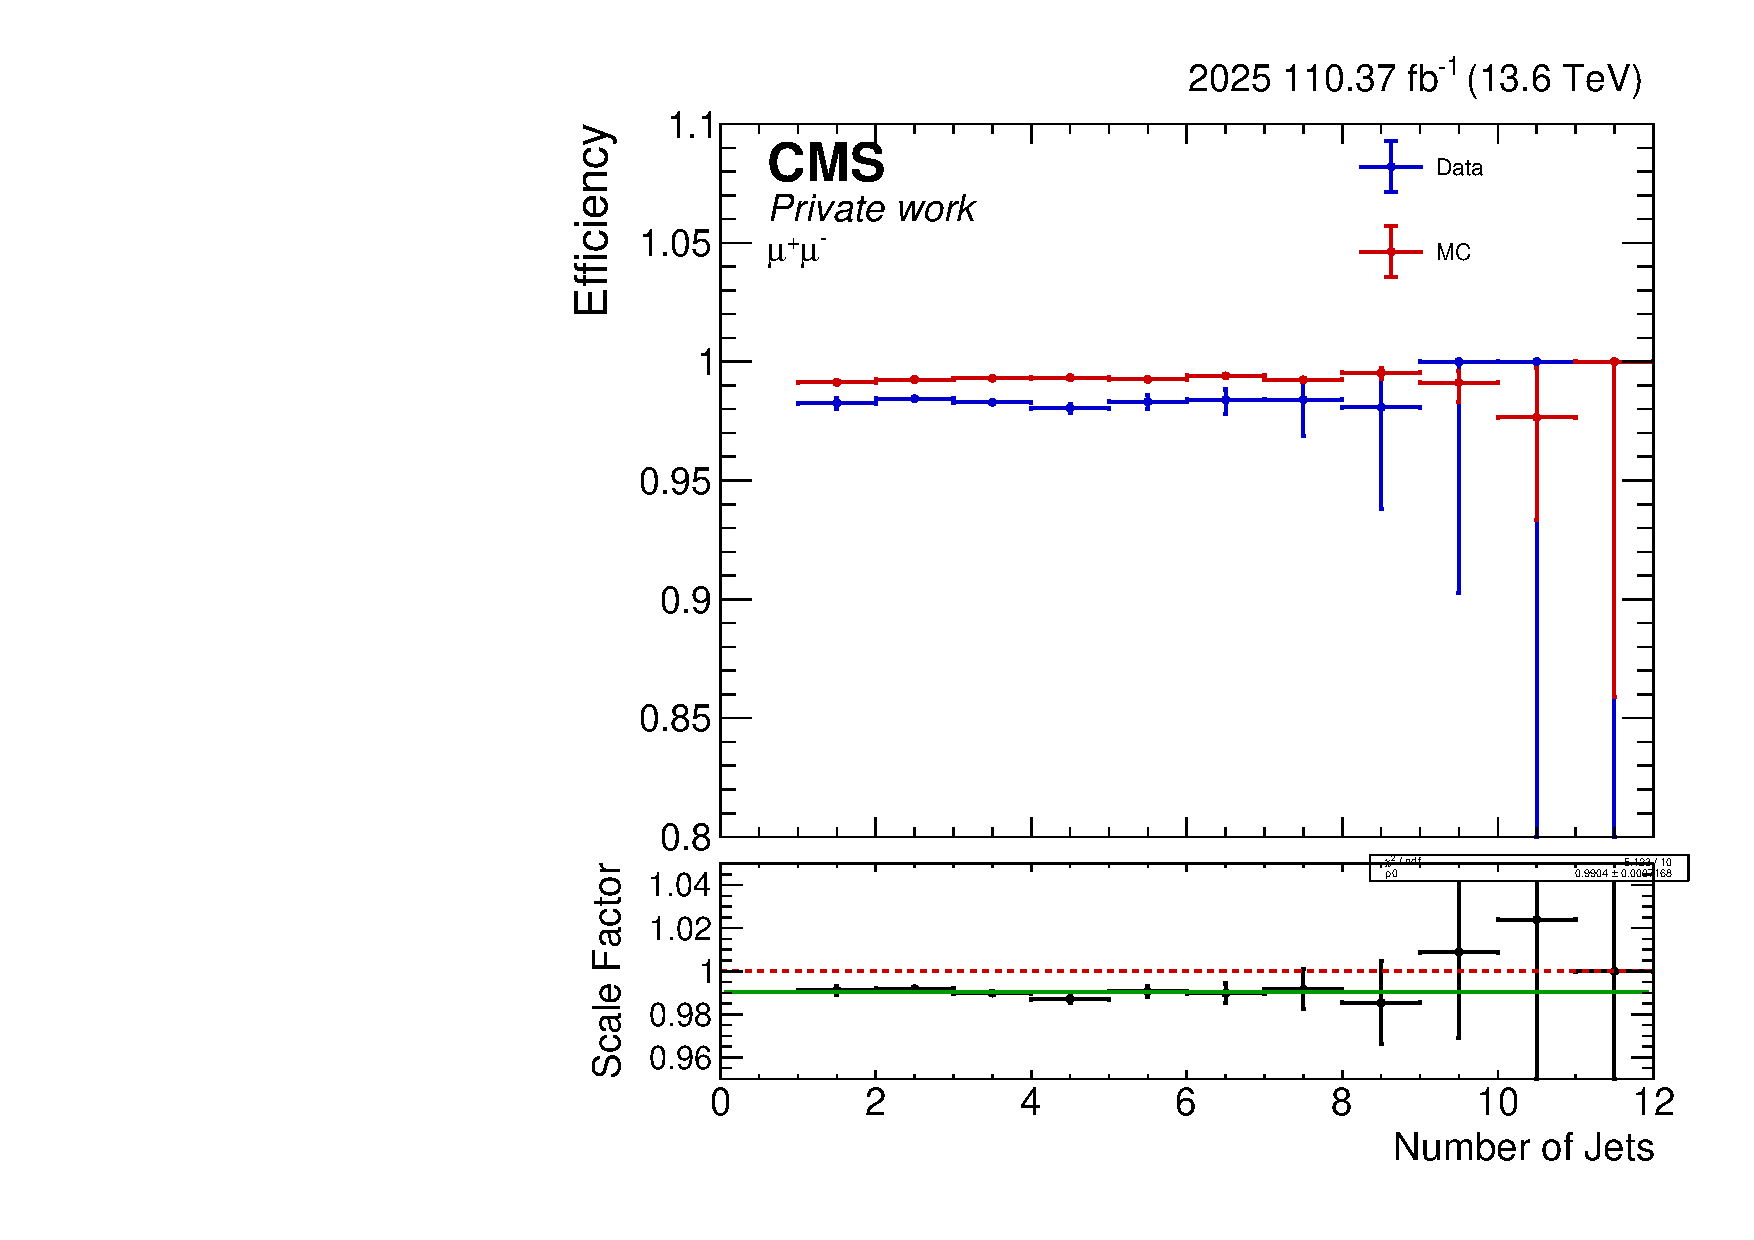
\includegraphics[width=0.48\linewidth]{figures/2025/MuMu/ScaleFactor/SF_Num_Jets.pdf}
\caption{Additional one-dimensional efficiency and SF diagnostics in the $\mu\mu$ channel. Variables and binning are shown on each axis.}\label{fig:diag-MuMu-SF_METpt-2025}
\end{figure}
\begin{figure}[htbp]\centering
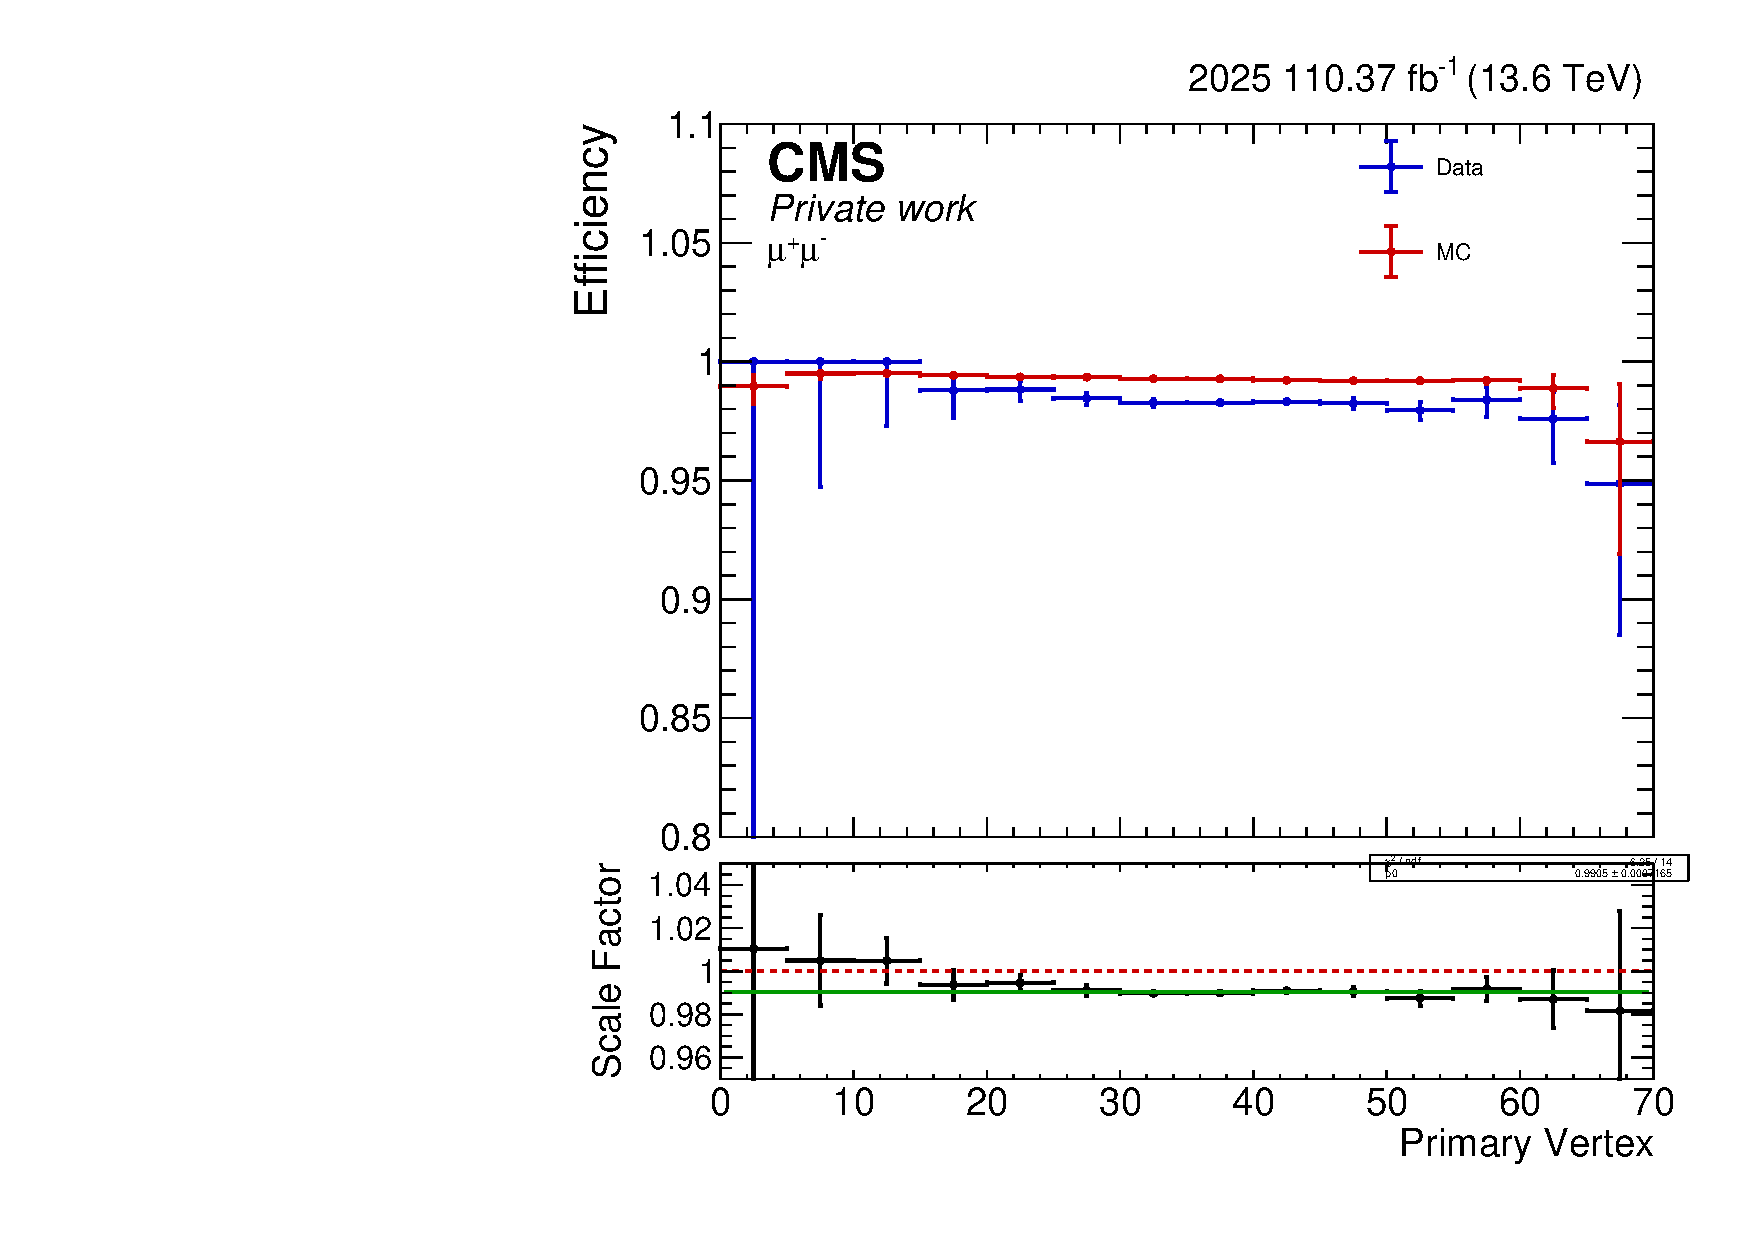
\includegraphics[width=0.48\linewidth]{figures/2025/MuMu/ScaleFactor/SF_Num_PV.pdf}
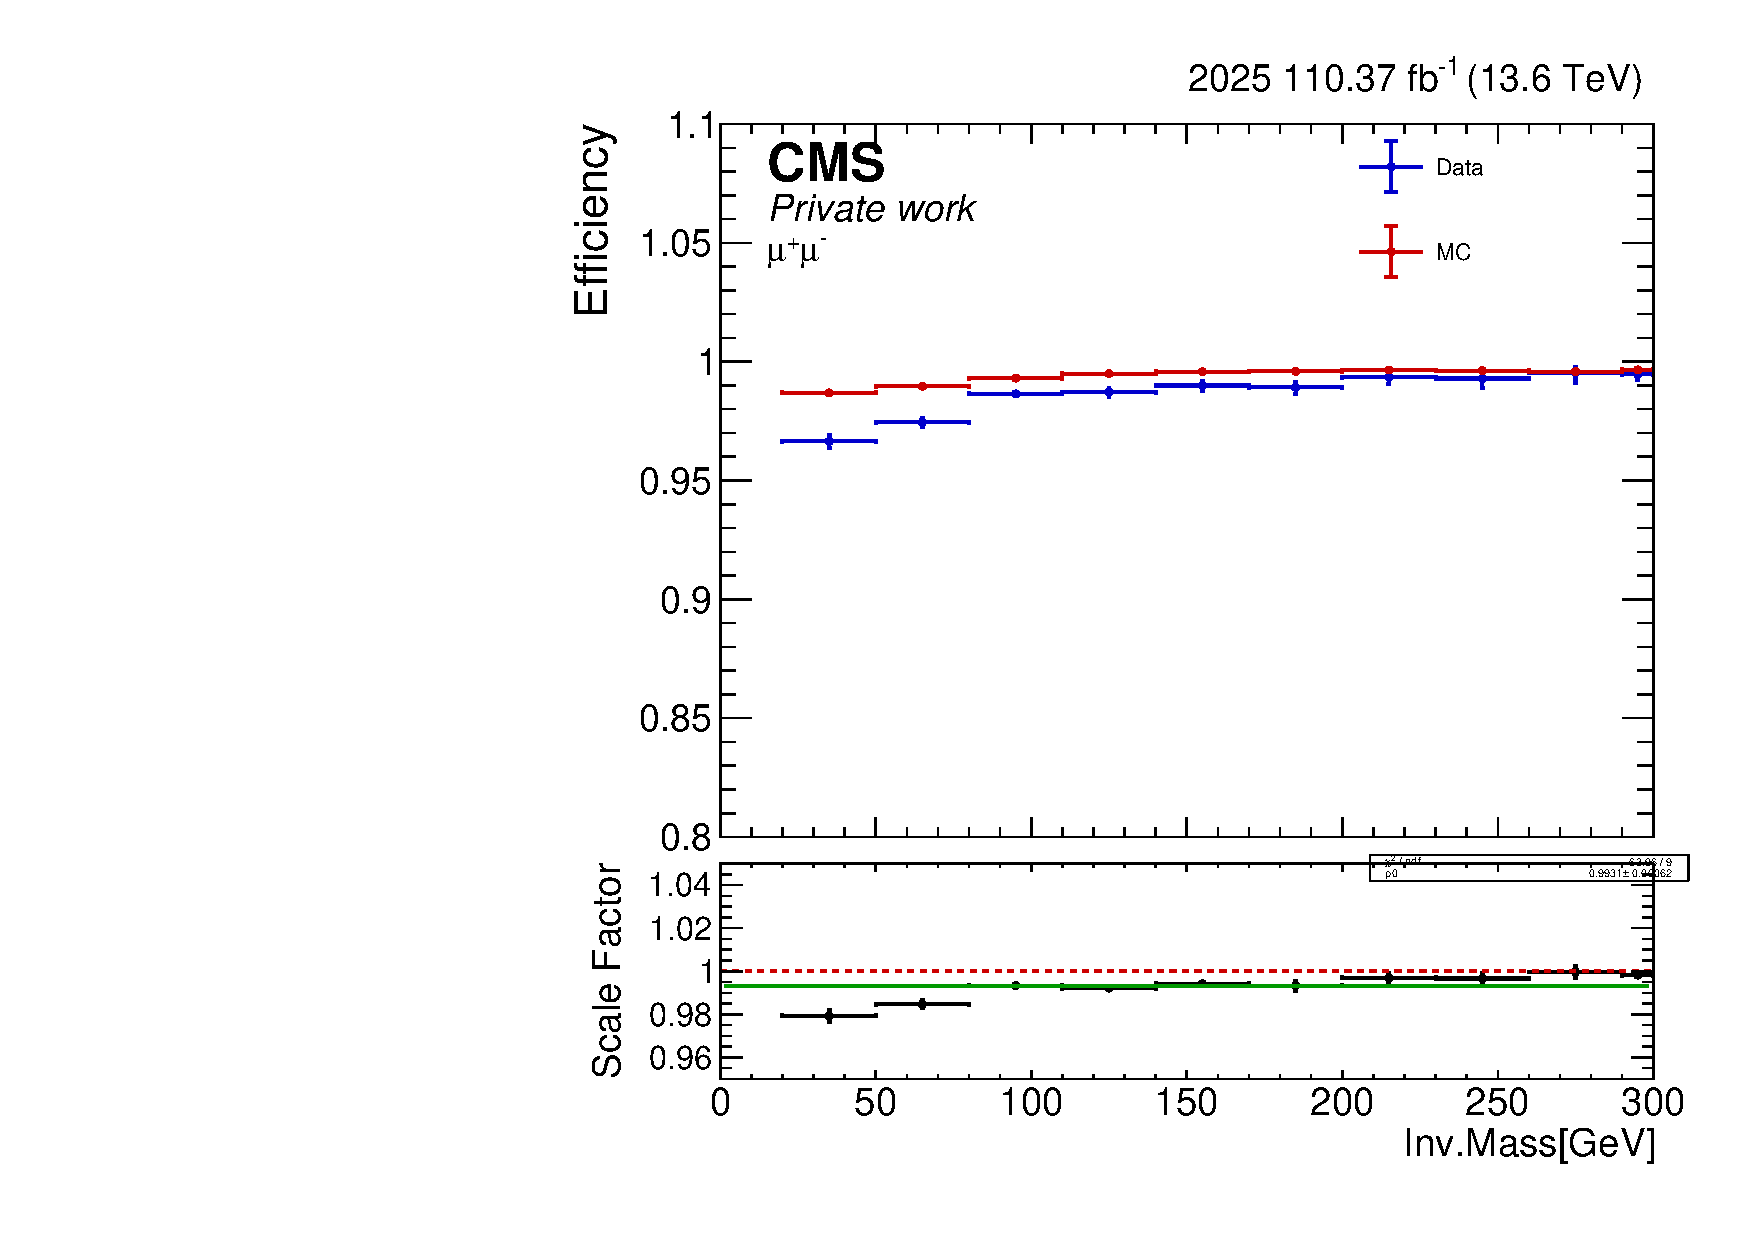
\includegraphics[width=0.48\linewidth]{figures/2025/MuMu/ScaleFactor/SF_DiLepMass.pdf}
\caption{Additional one-dimensional efficiency and SF diagnostics in the $\mu\mu$ channel. Variables and binning are shown on each axis.}\label{fig:diag-MuMu-SF_Num_PV-2025}
\end{figure}
\clearpage\section{2025: detailed uncertainty studies}\label{app:studies-2025}
\begin{figure}[htbp]\centering
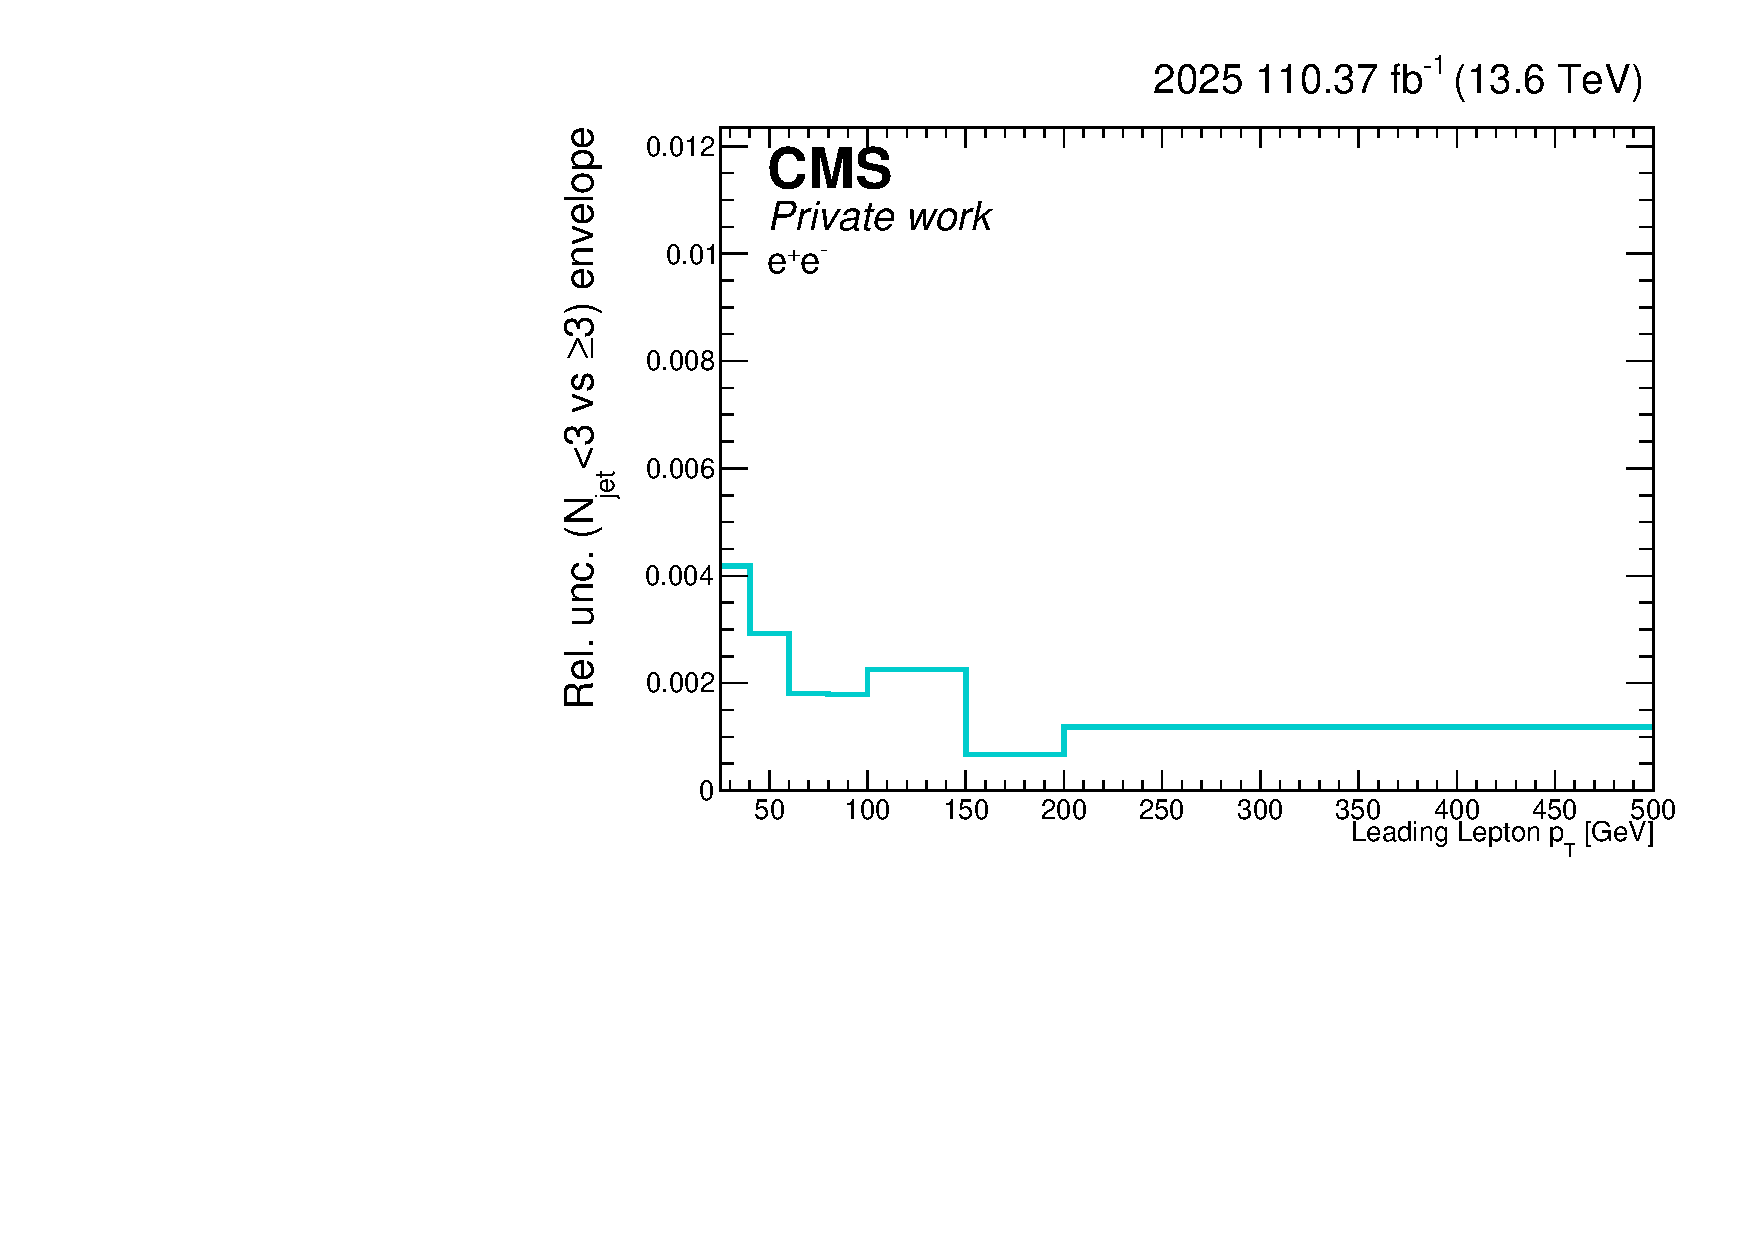
\includegraphics[width=0.48\linewidth]{figures/2025/ElEl/Jet_Topology_Uncertainty/TopoJetUnc_Lep1pt.pdf}
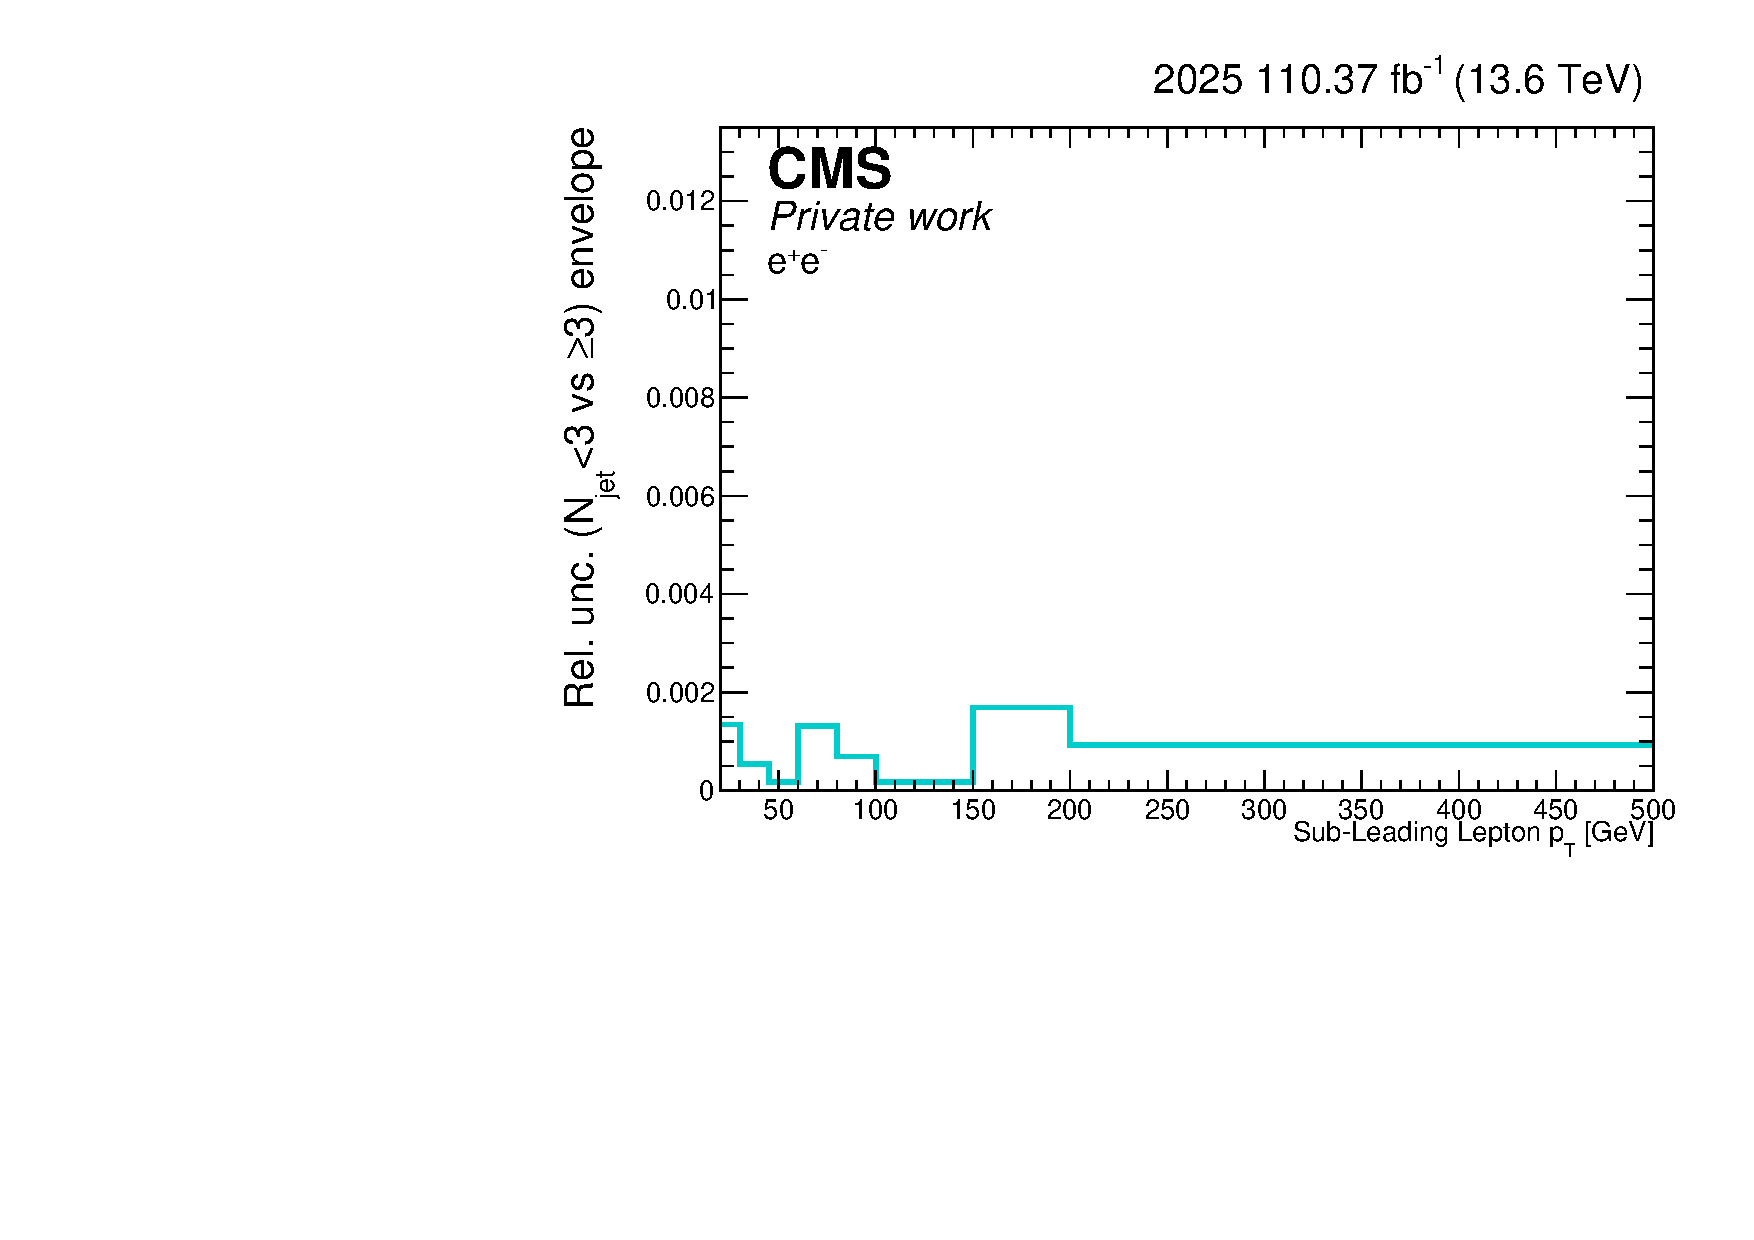
\includegraphics[width=0.48\linewidth]{figures/2025/ElEl/Jet_Topology_Uncertainty/TopoJetUnc_Lep2pt.pdf}
\caption{Jet Topology Uncertainty diagnostics in the $ee$ channel versus leading and subleading lepton momentum. Curves are reproduced with the production definitions; their exact numerical prescription requires confirmation.}\label{fig:study-ElEl-TopoJetUnc-2025}
\end{figure}
\begin{figure}[htbp]\centering
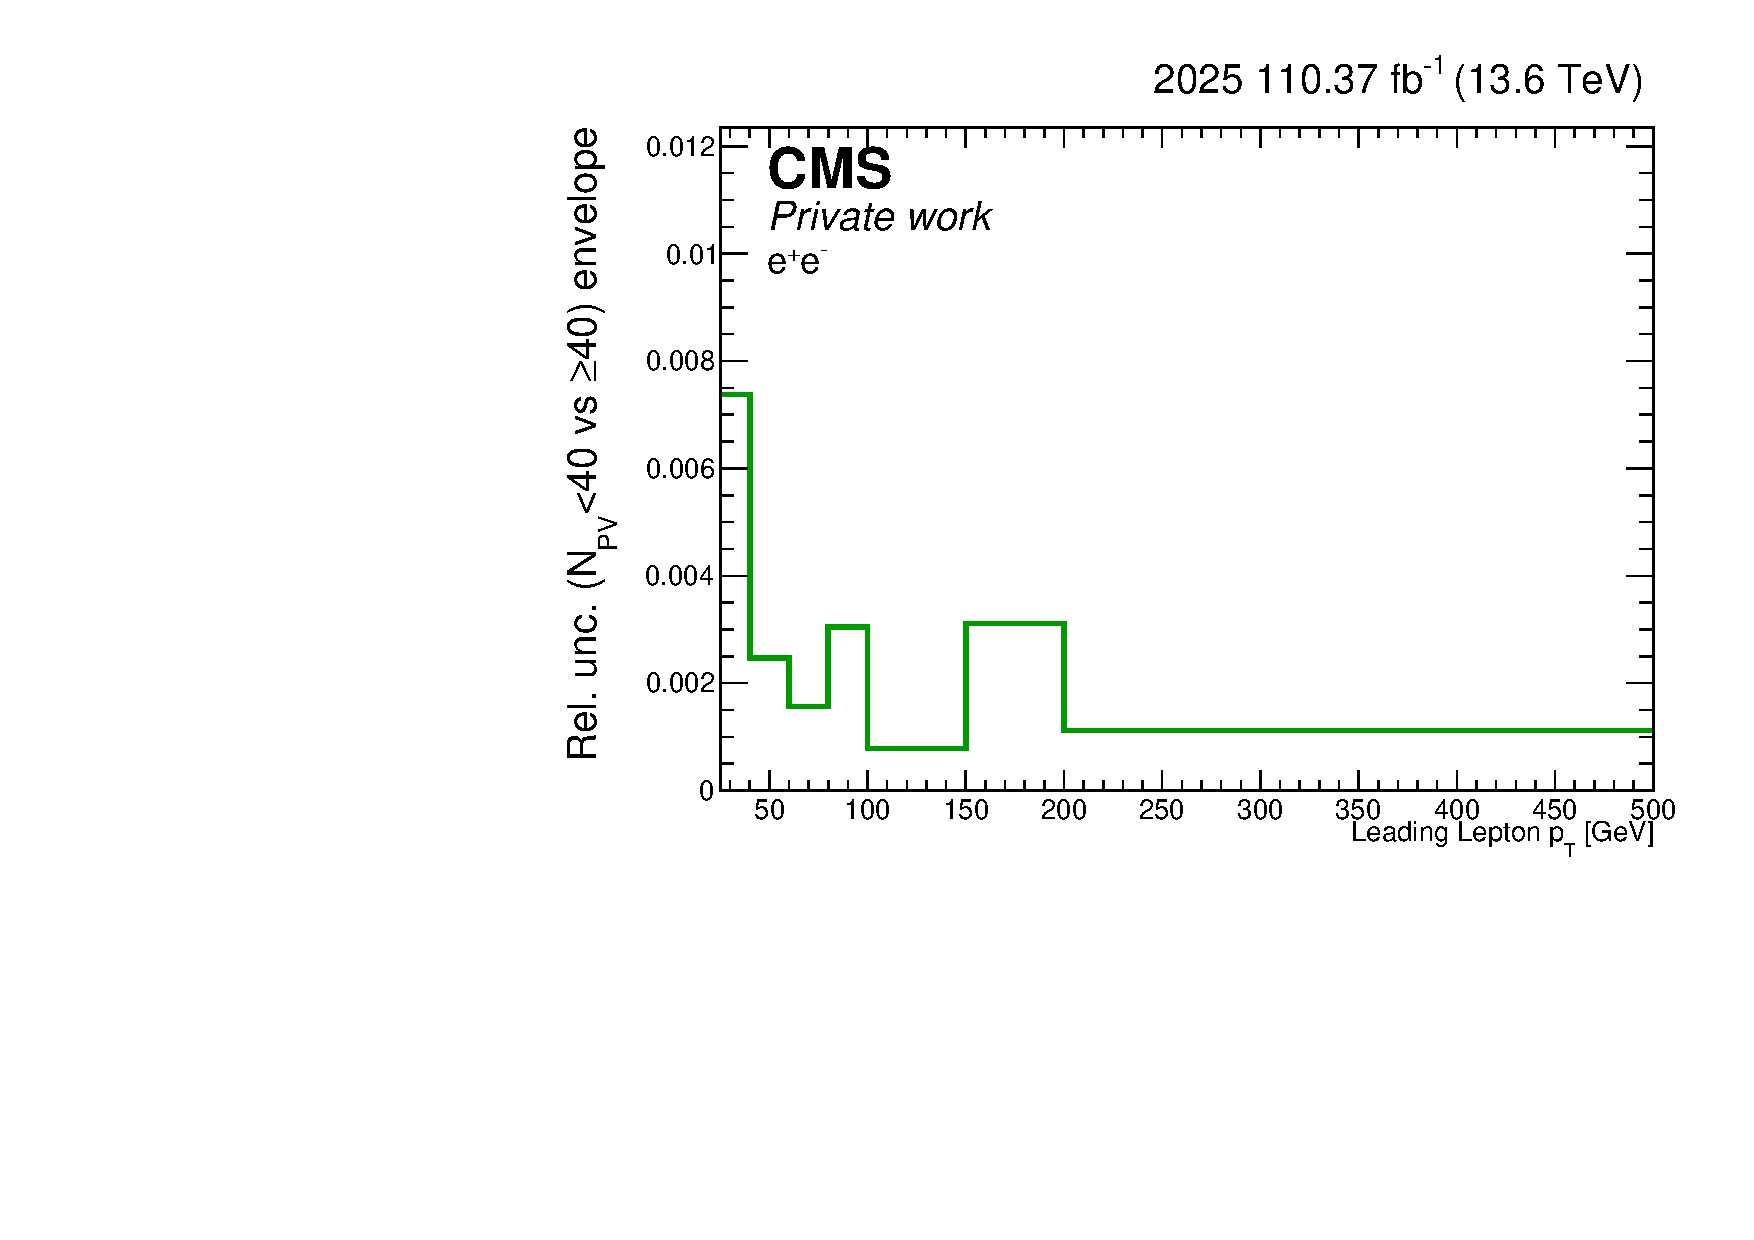
\includegraphics[width=0.48\linewidth]{figures/2025/ElEl/PV_Topology_Uncertainty/TopoPVUnc_Lep1pt.pdf}
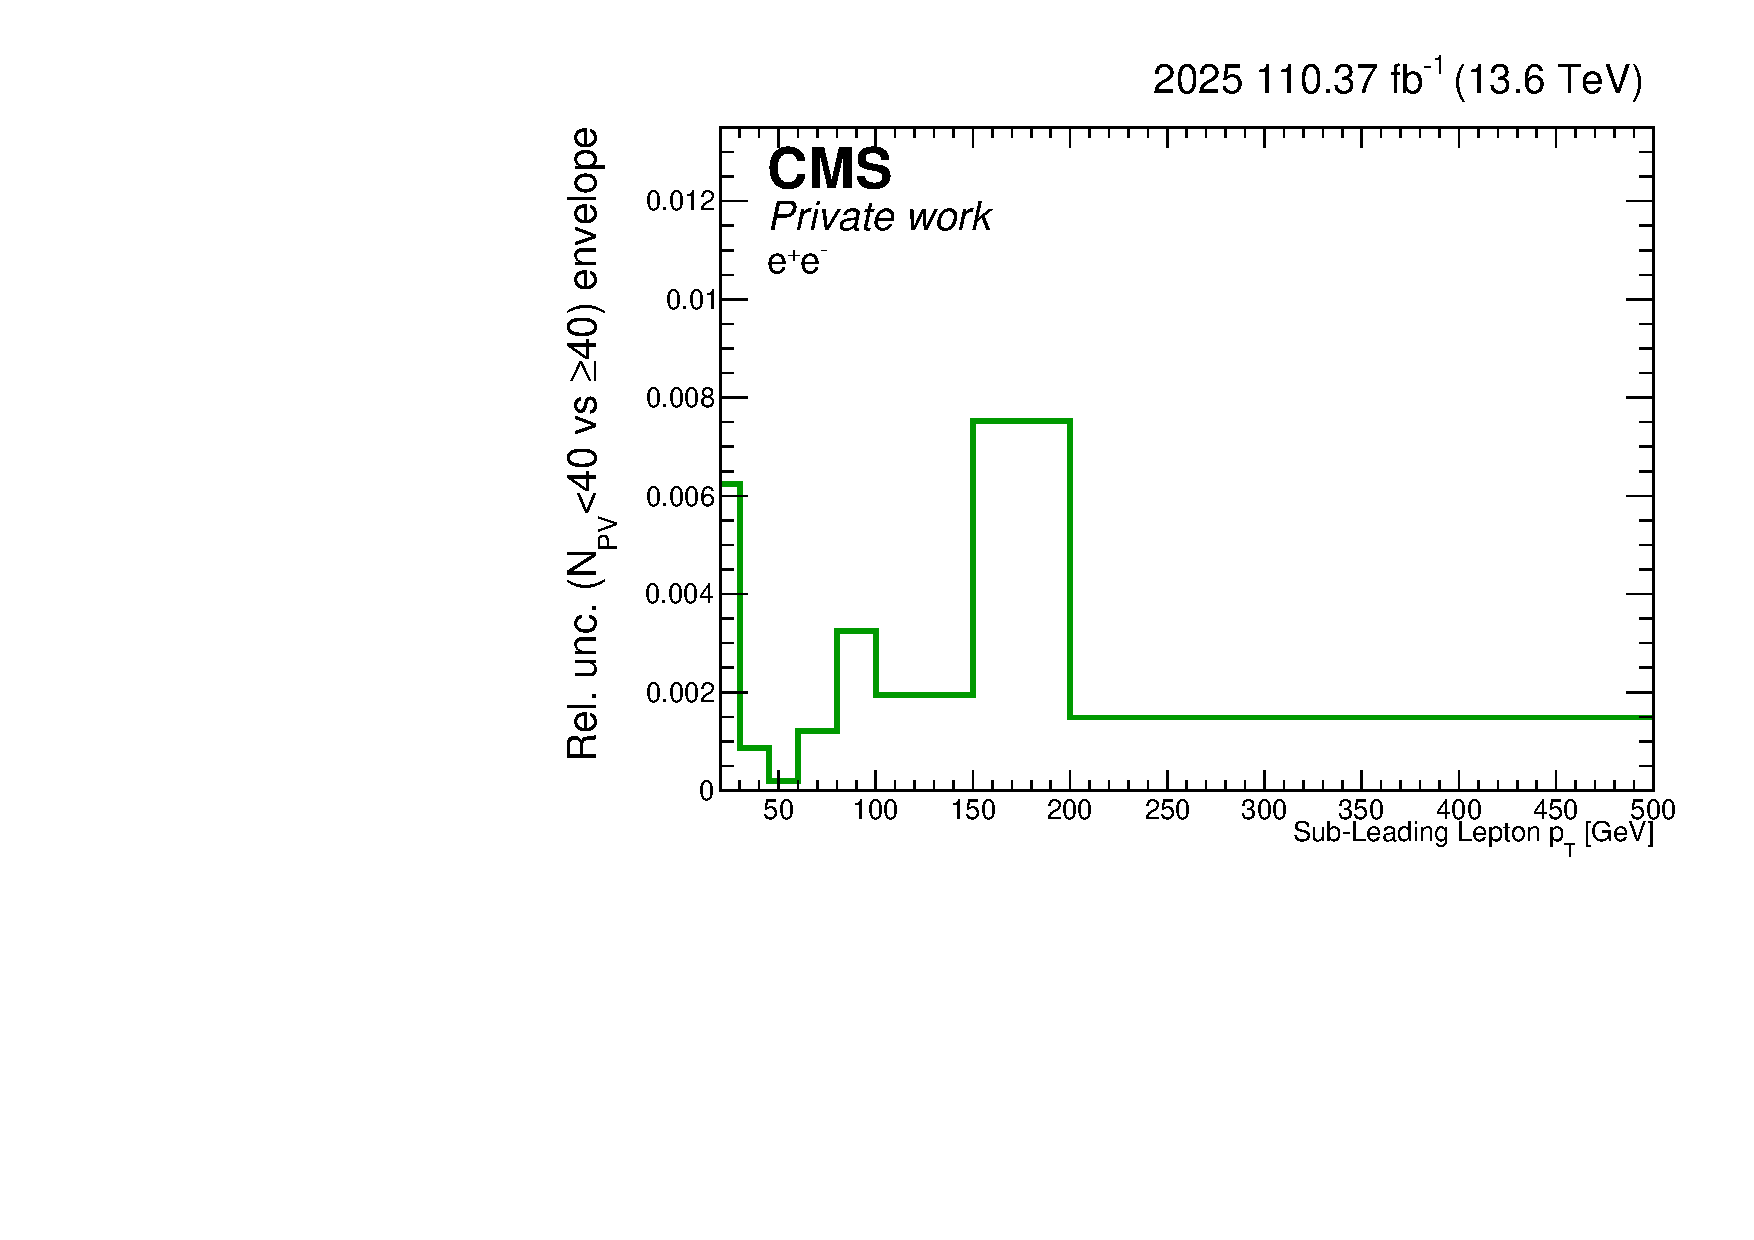
\includegraphics[width=0.48\linewidth]{figures/2025/ElEl/PV_Topology_Uncertainty/TopoPVUnc_Lep2pt.pdf}
\caption{PV Topology Uncertainty diagnostics in the $ee$ channel versus leading and subleading lepton momentum. Curves are reproduced with the production definitions; their exact numerical prescription requires confirmation.}\label{fig:study-ElEl-TopoPVUnc-2025}
\end{figure}
\begin{figure}[htbp]\centering
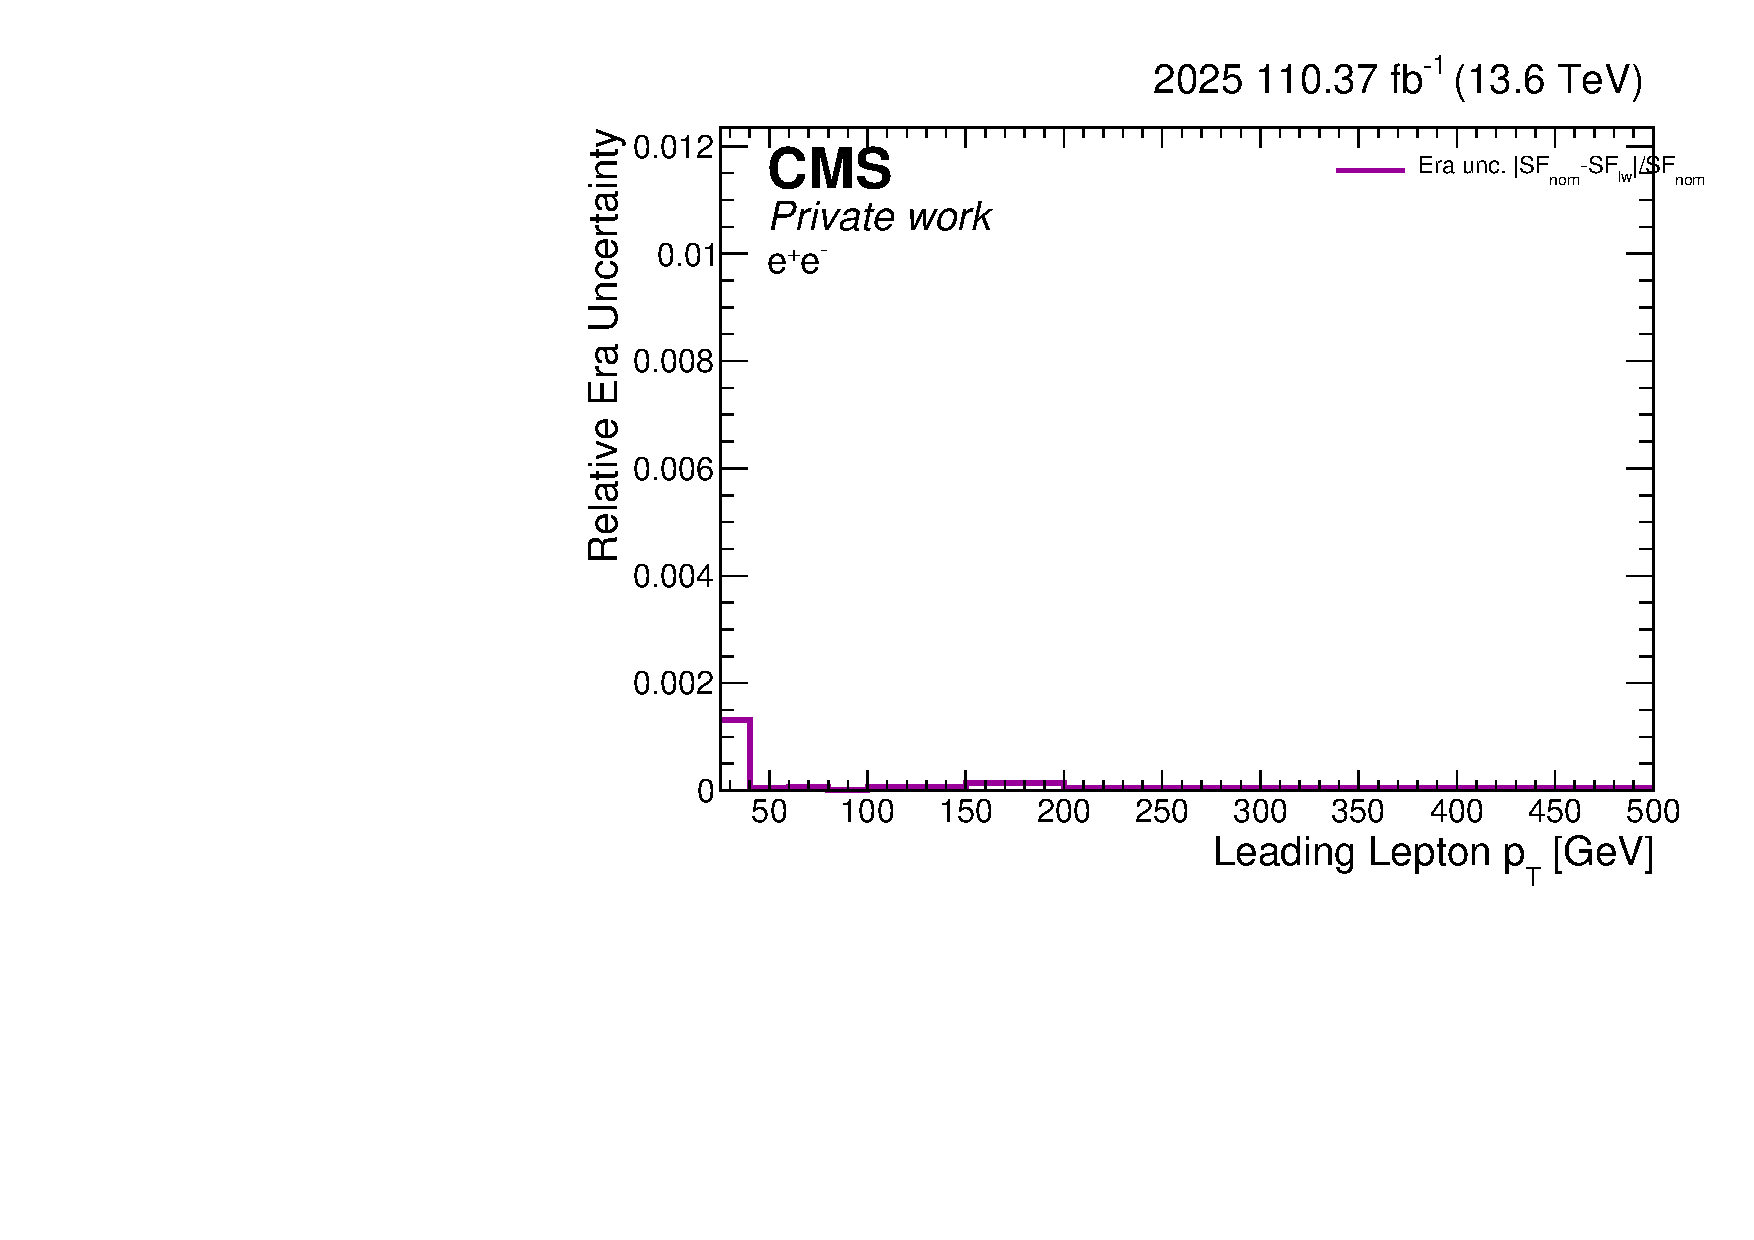
\includegraphics[width=0.48\linewidth]{figures/2025/ElEl/Era_Uncertainty/EraUnc_Lep1pt.pdf}
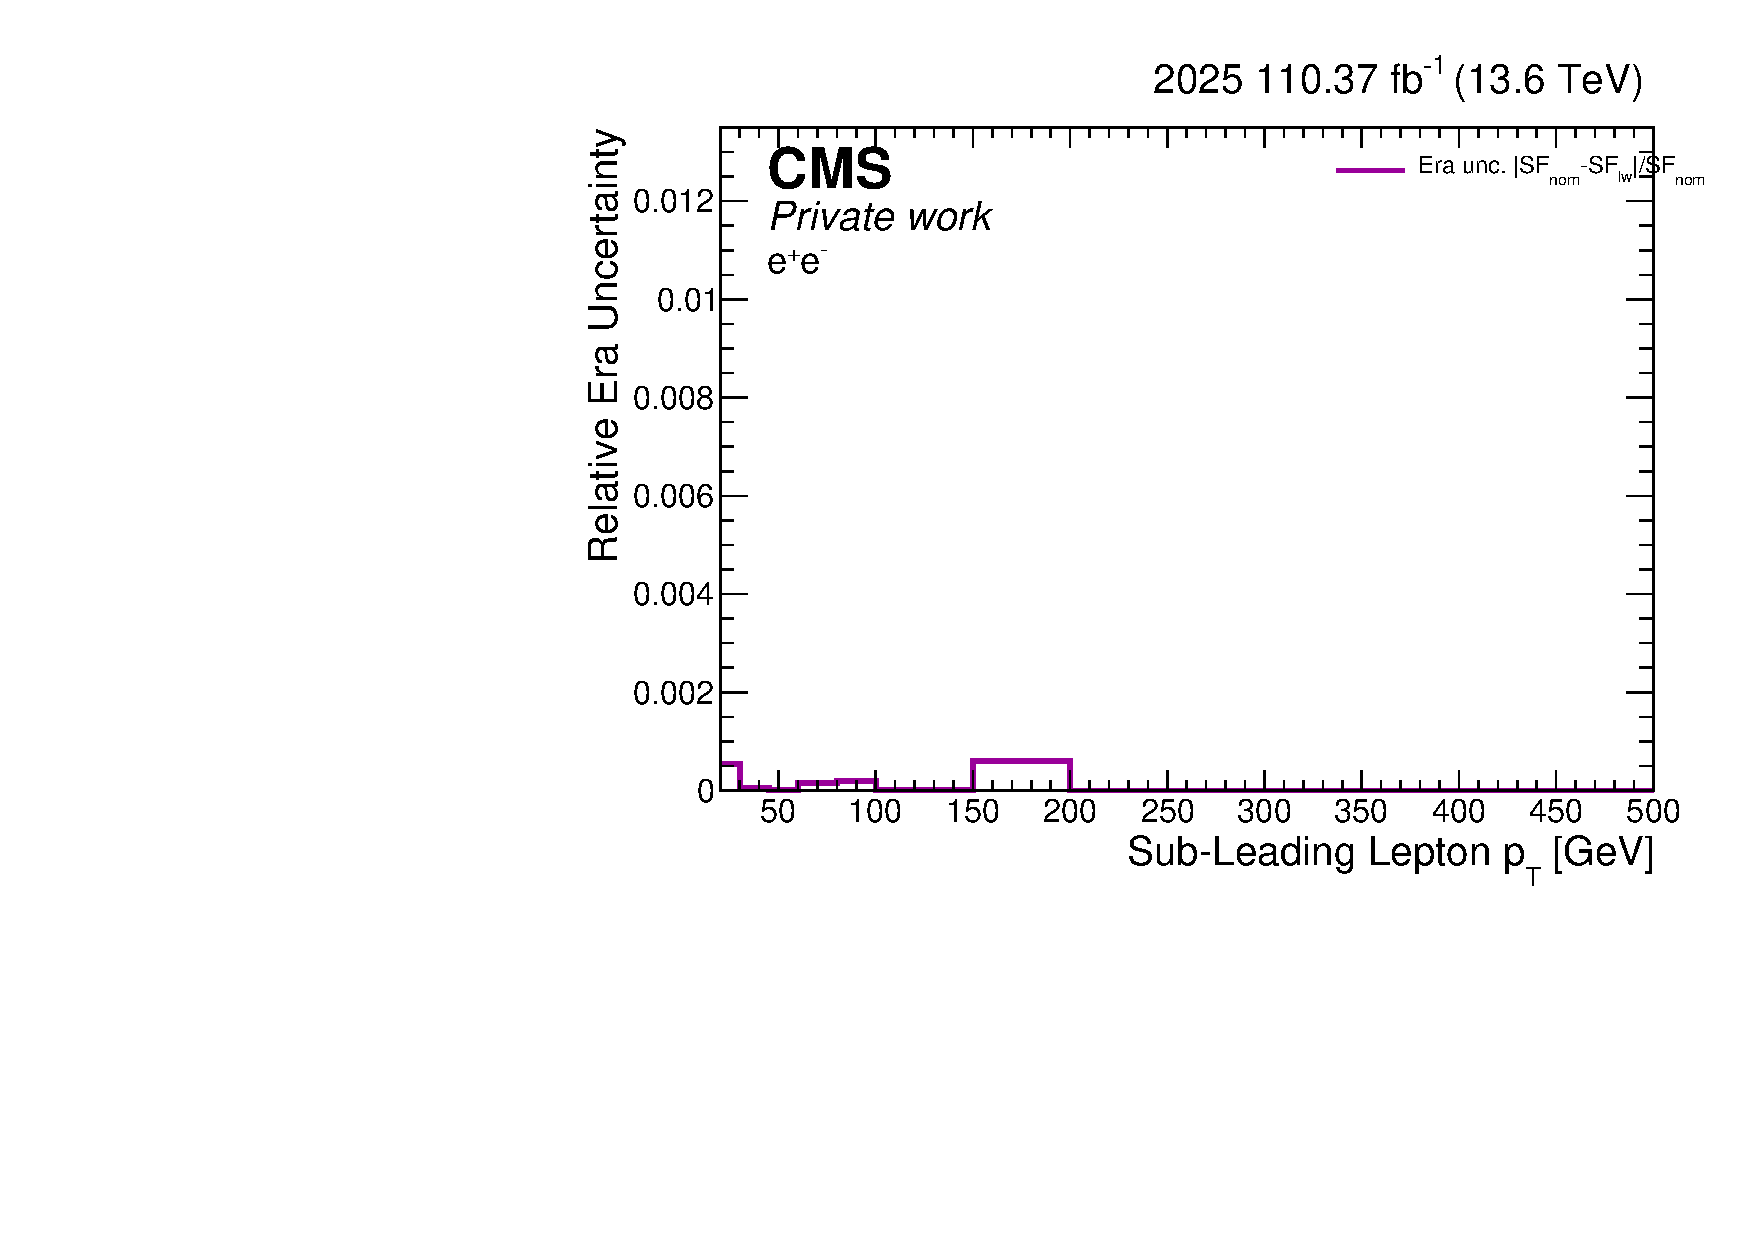
\includegraphics[width=0.48\linewidth]{figures/2025/ElEl/Era_Uncertainty/EraUnc_Lep2pt.pdf}
\caption{Era Uncertainty diagnostics in the $ee$ channel versus leading and subleading lepton momentum. Curves are reproduced with the production definitions; their exact numerical prescription requires confirmation.}\label{fig:study-ElEl-EraUnc-2025}
\end{figure}
\begin{figure}[htbp]\centering
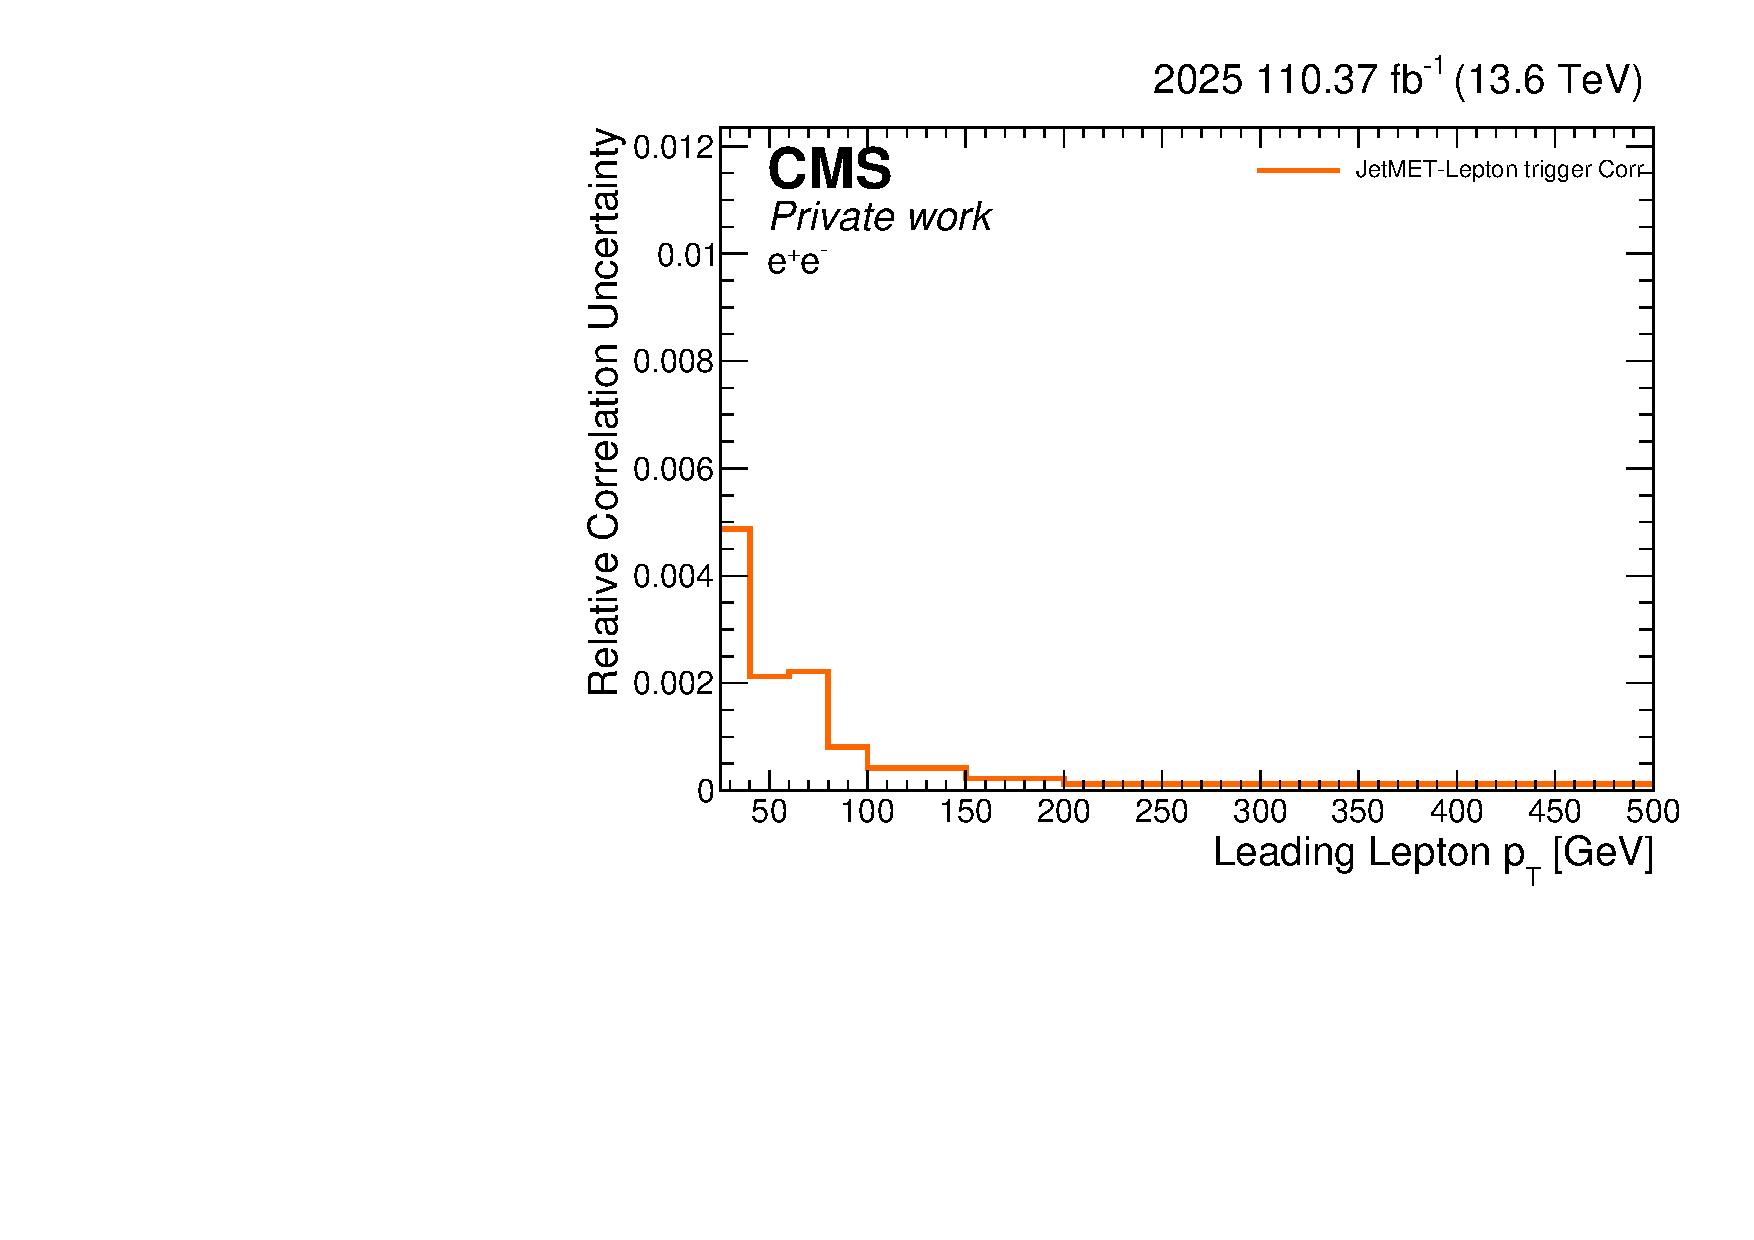
\includegraphics[width=0.48\linewidth]{figures/2025/ElEl/Correlation_Uncertainty/CorrUnc_Lep1pt.pdf}
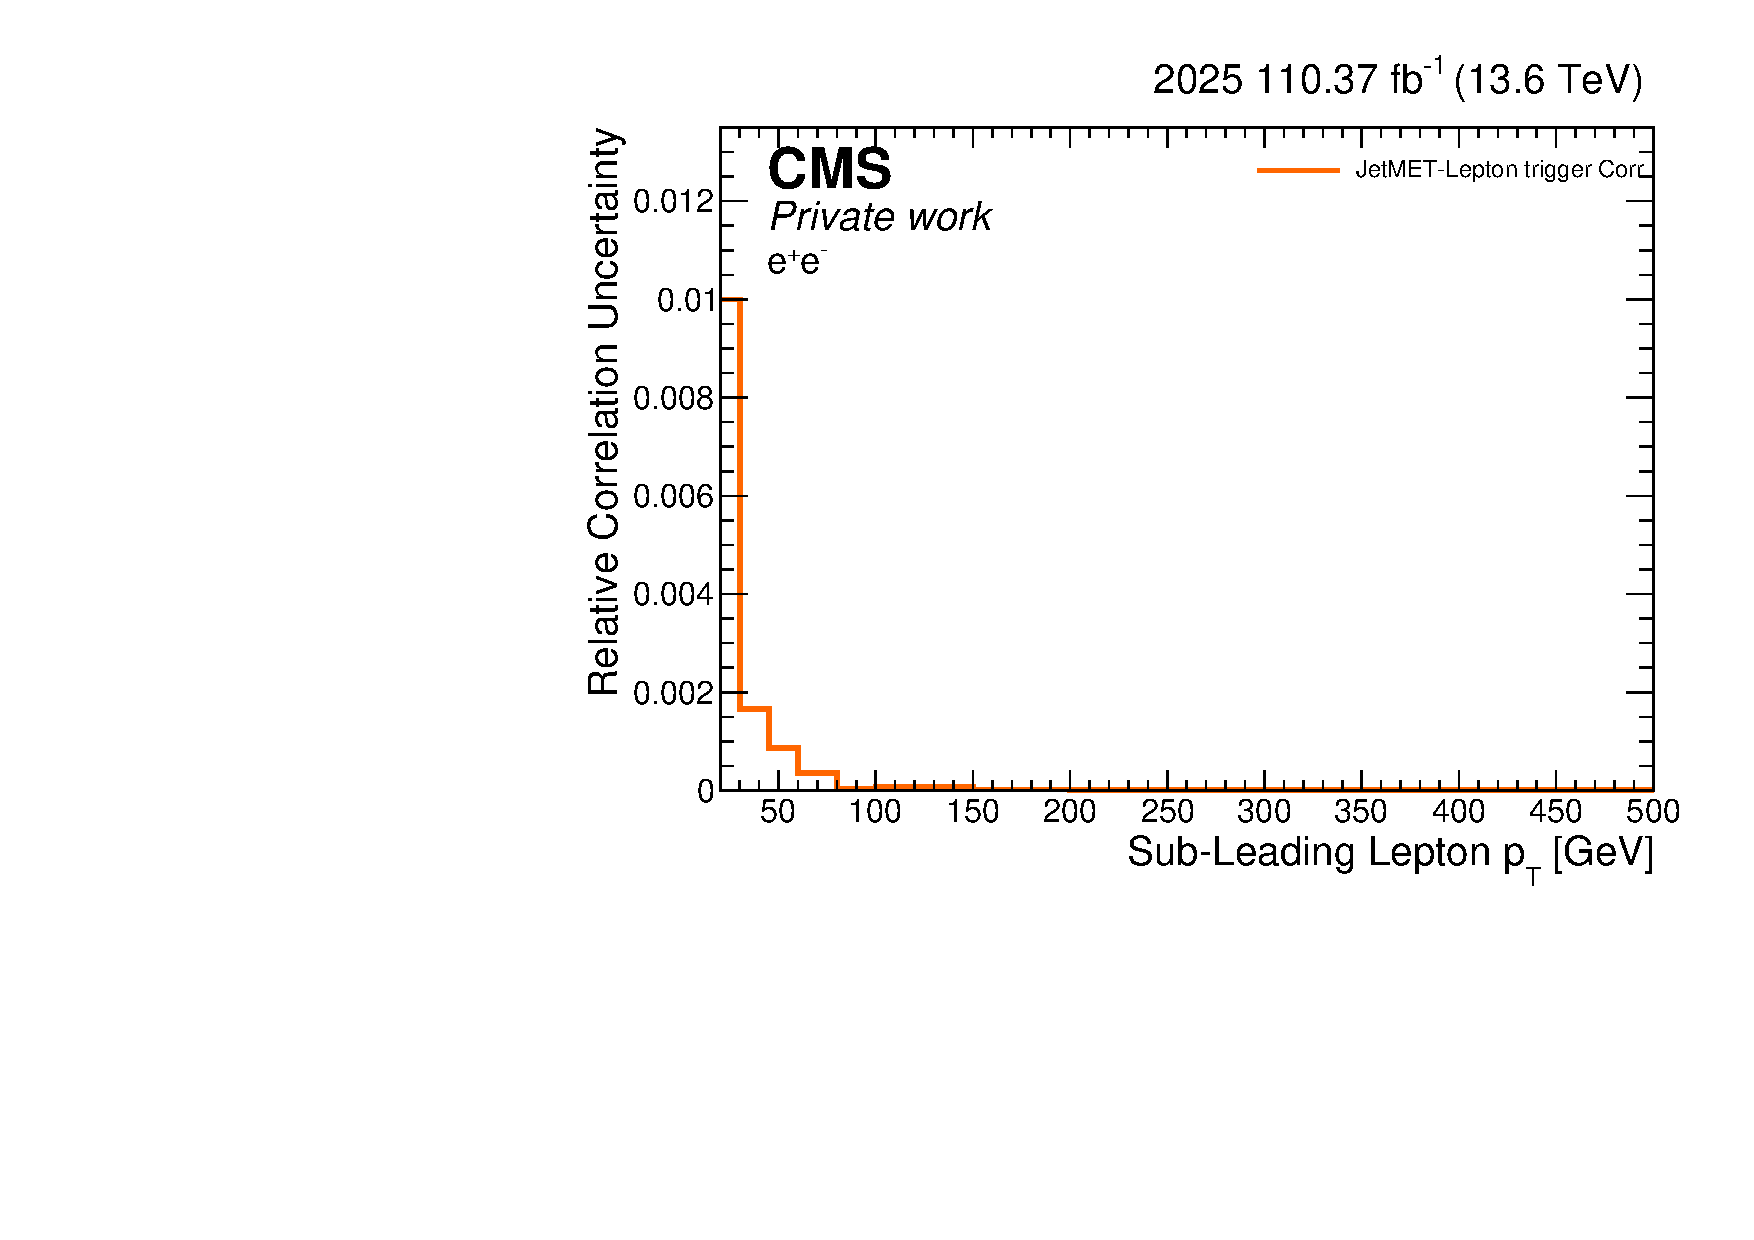
\includegraphics[width=0.48\linewidth]{figures/2025/ElEl/Correlation_Uncertainty/CorrUnc_Lep2pt.pdf}
\caption{Correlation Uncertainty diagnostics in the $ee$ channel versus leading and subleading lepton momentum. Curves are reproduced with the production definitions; their exact numerical prescription requires confirmation.}\label{fig:study-ElEl-CorrUnc-2025}
\end{figure}
\begin{figure}[htbp]\centering
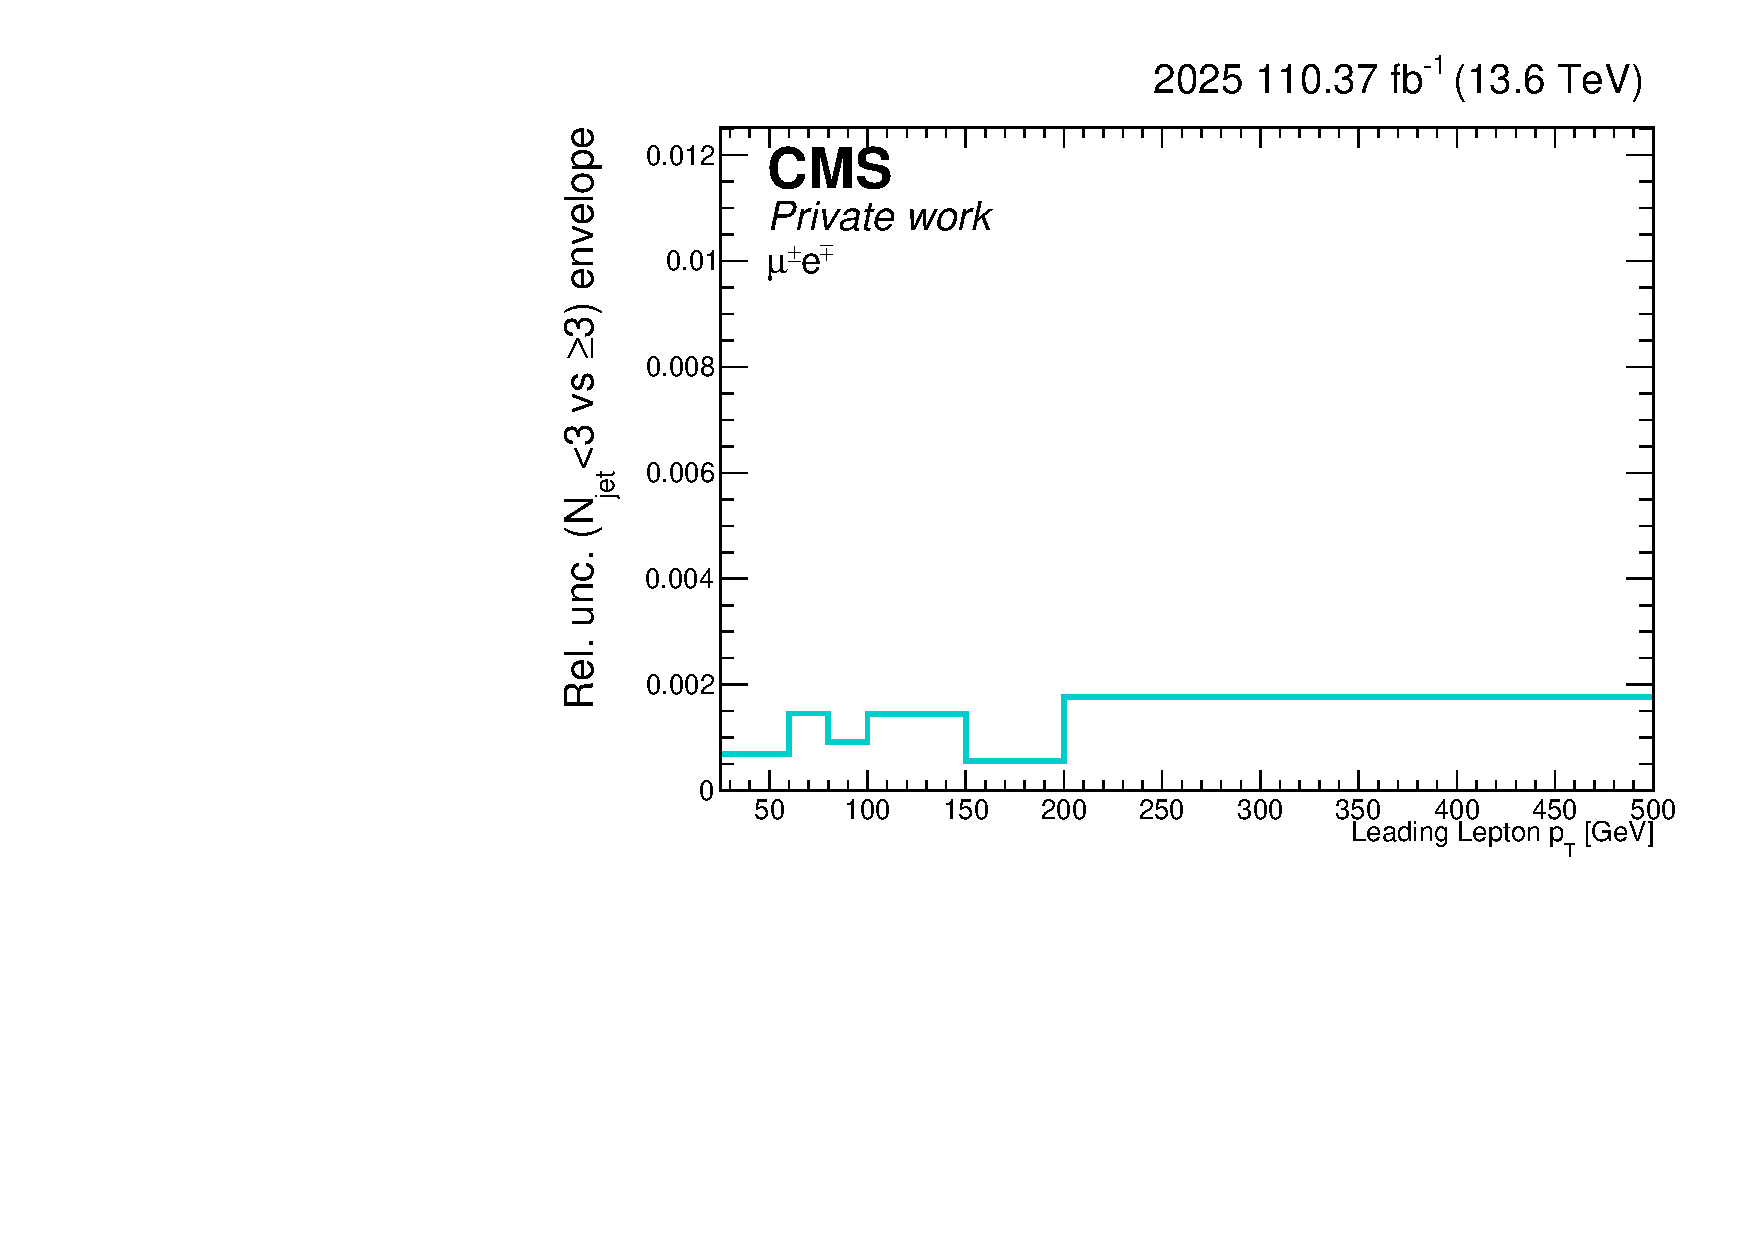
\includegraphics[width=0.48\linewidth]{figures/2025/MuEl/Jet_Topology_Uncertainty/TopoJetUnc_Lep1pt.pdf}
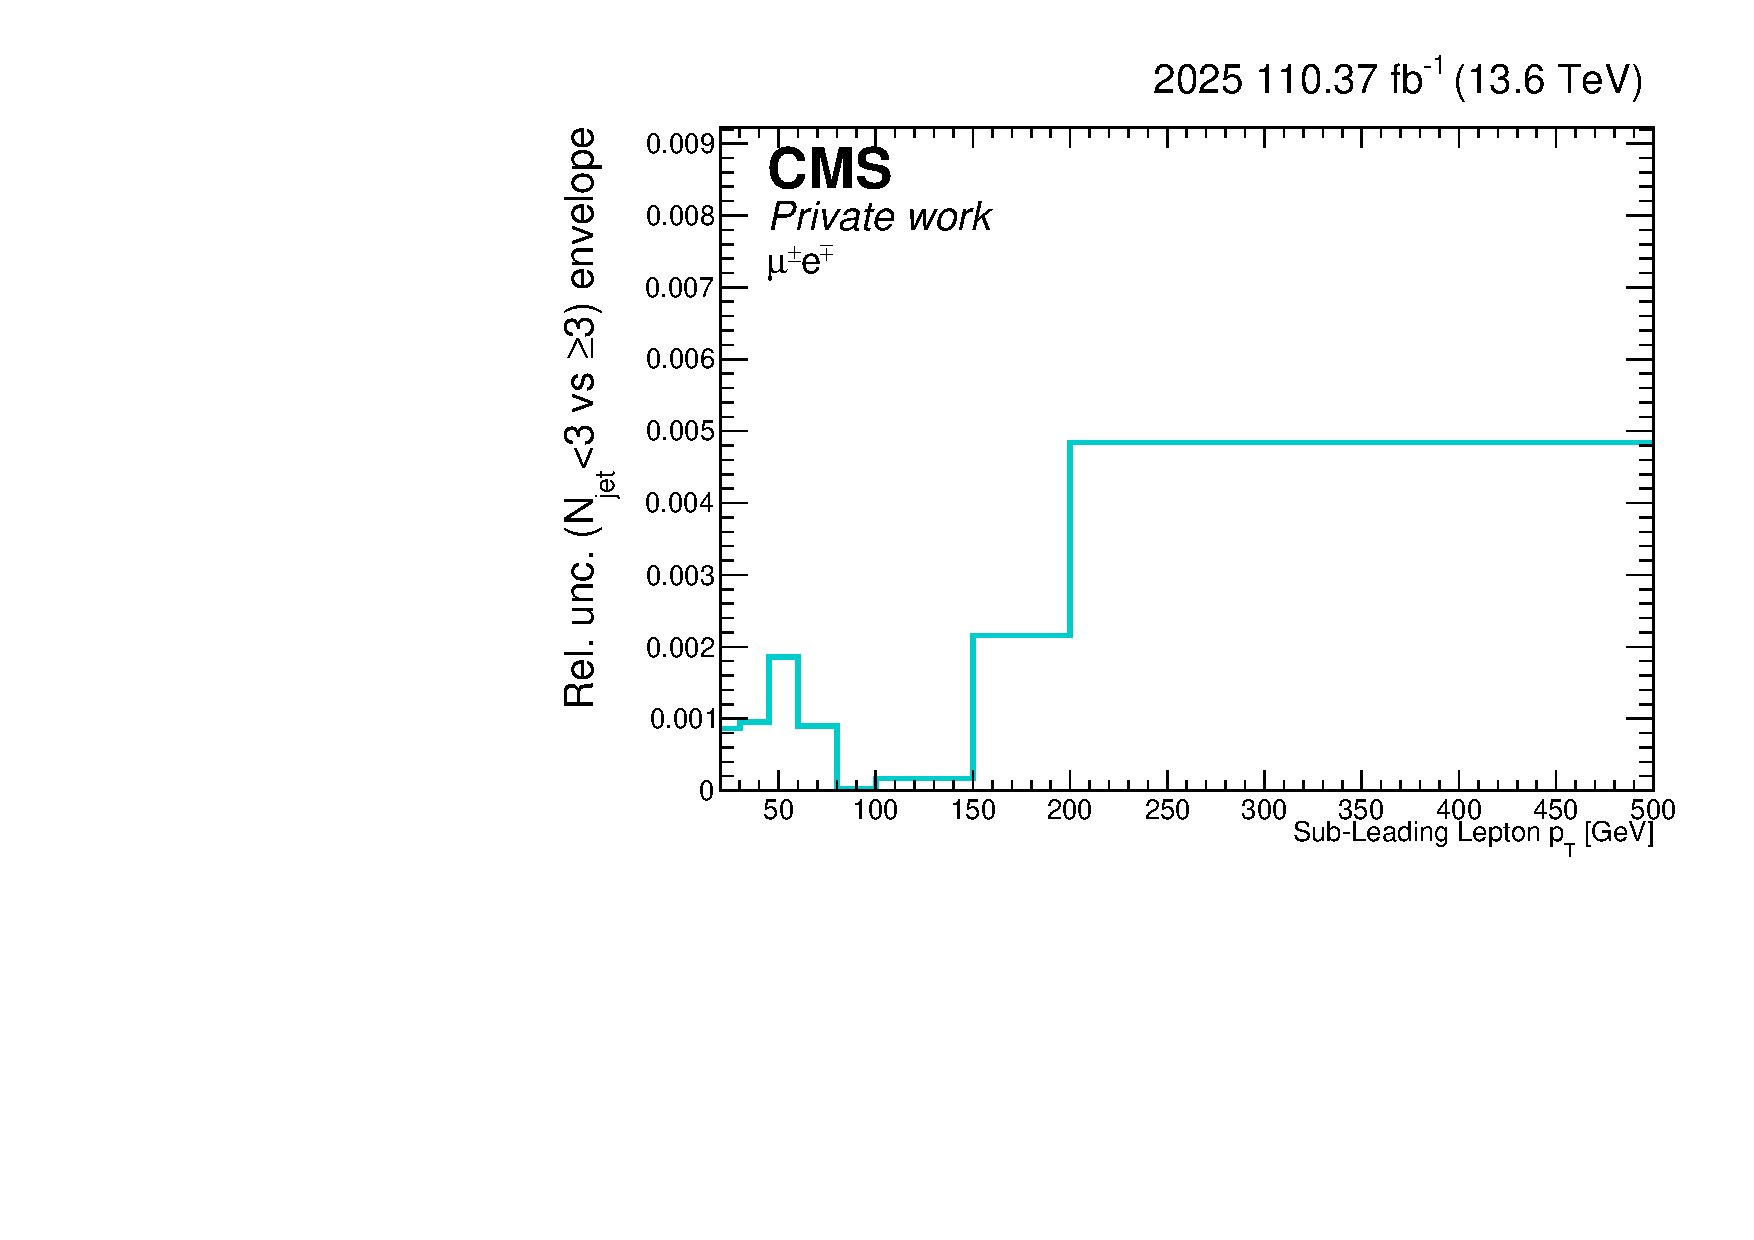
\includegraphics[width=0.48\linewidth]{figures/2025/MuEl/Jet_Topology_Uncertainty/TopoJetUnc_Lep2pt.pdf}
\caption{Jet Topology Uncertainty diagnostics in the $e\mu$ channel versus leading and subleading lepton momentum. Curves are reproduced with the production definitions; their exact numerical prescription requires confirmation.}\label{fig:study-MuEl-TopoJetUnc-2025}
\end{figure}
\begin{figure}[htbp]\centering
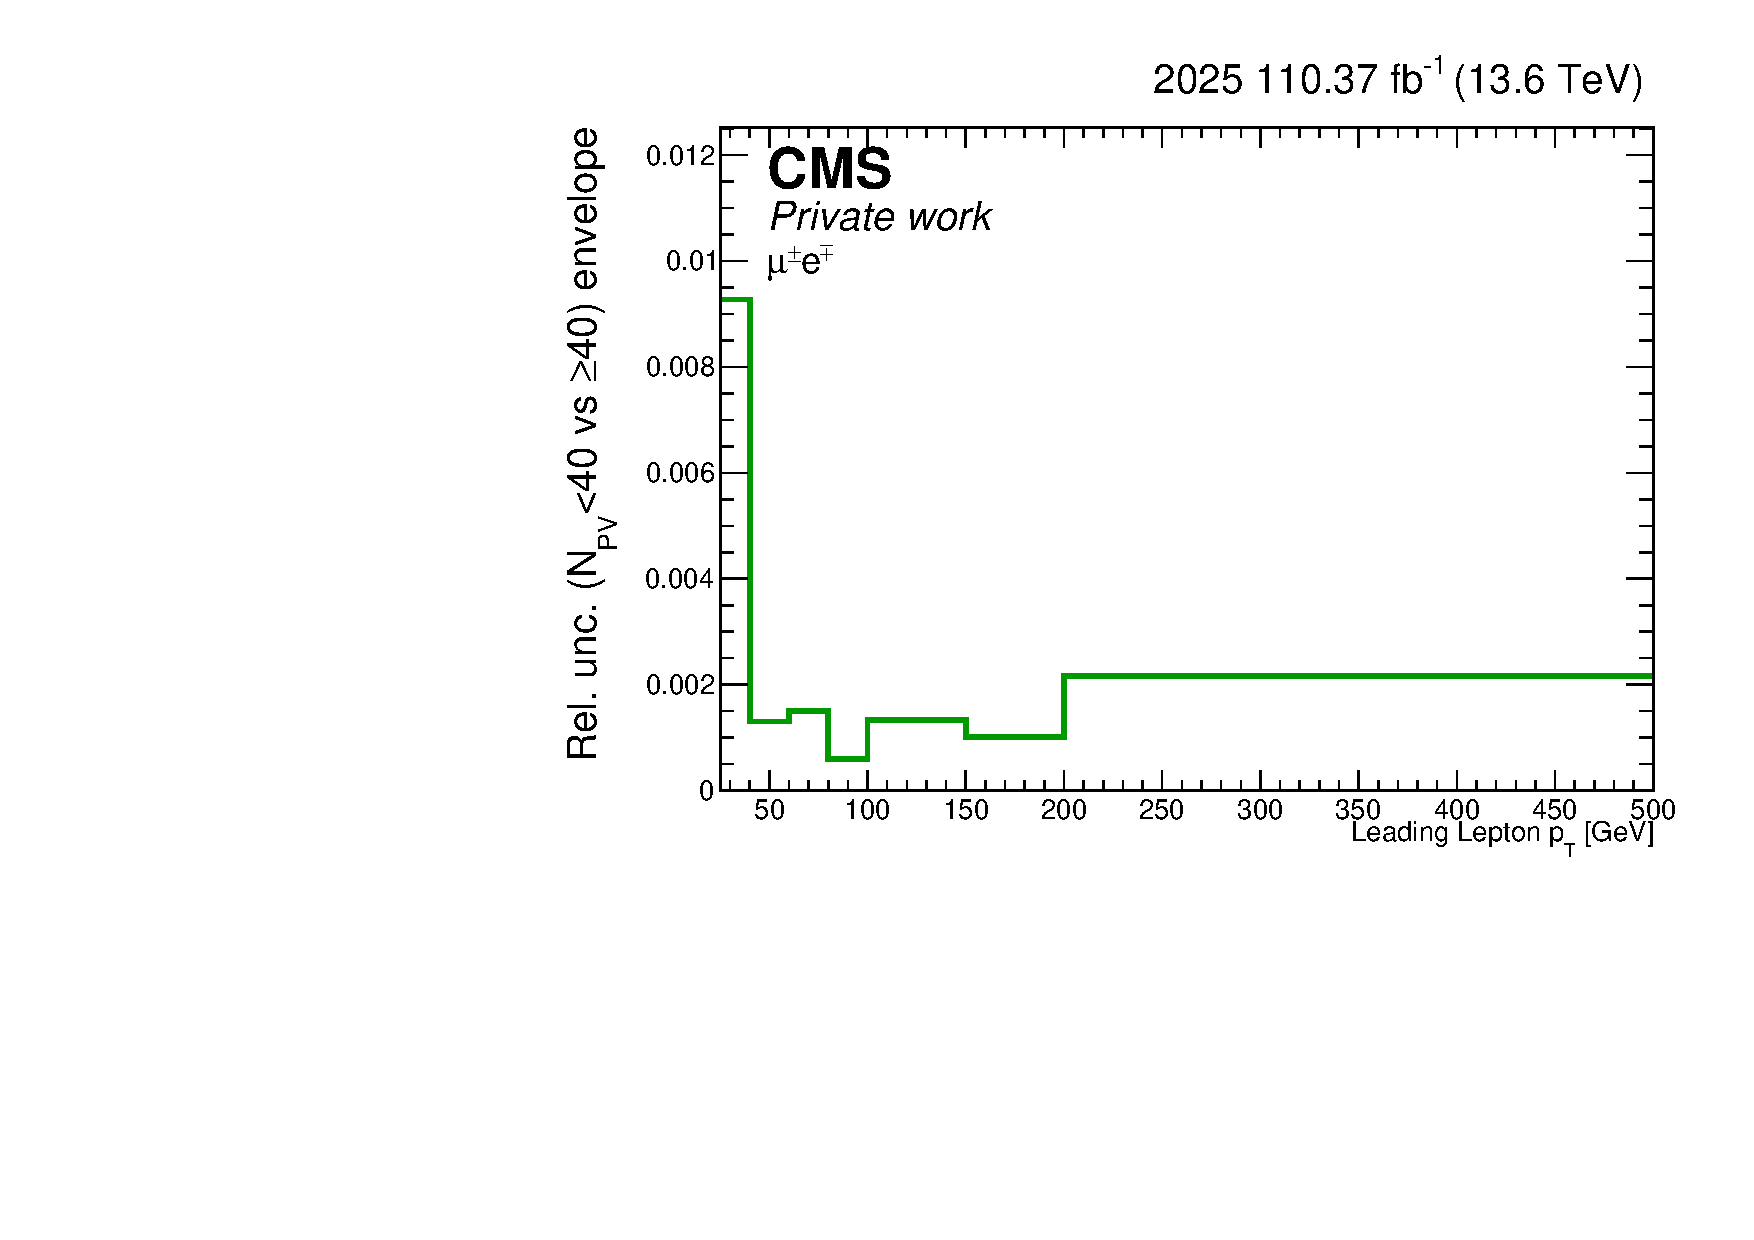
\includegraphics[width=0.48\linewidth]{figures/2025/MuEl/PV_Topology_Uncertainty/TopoPVUnc_Lep1pt.pdf}
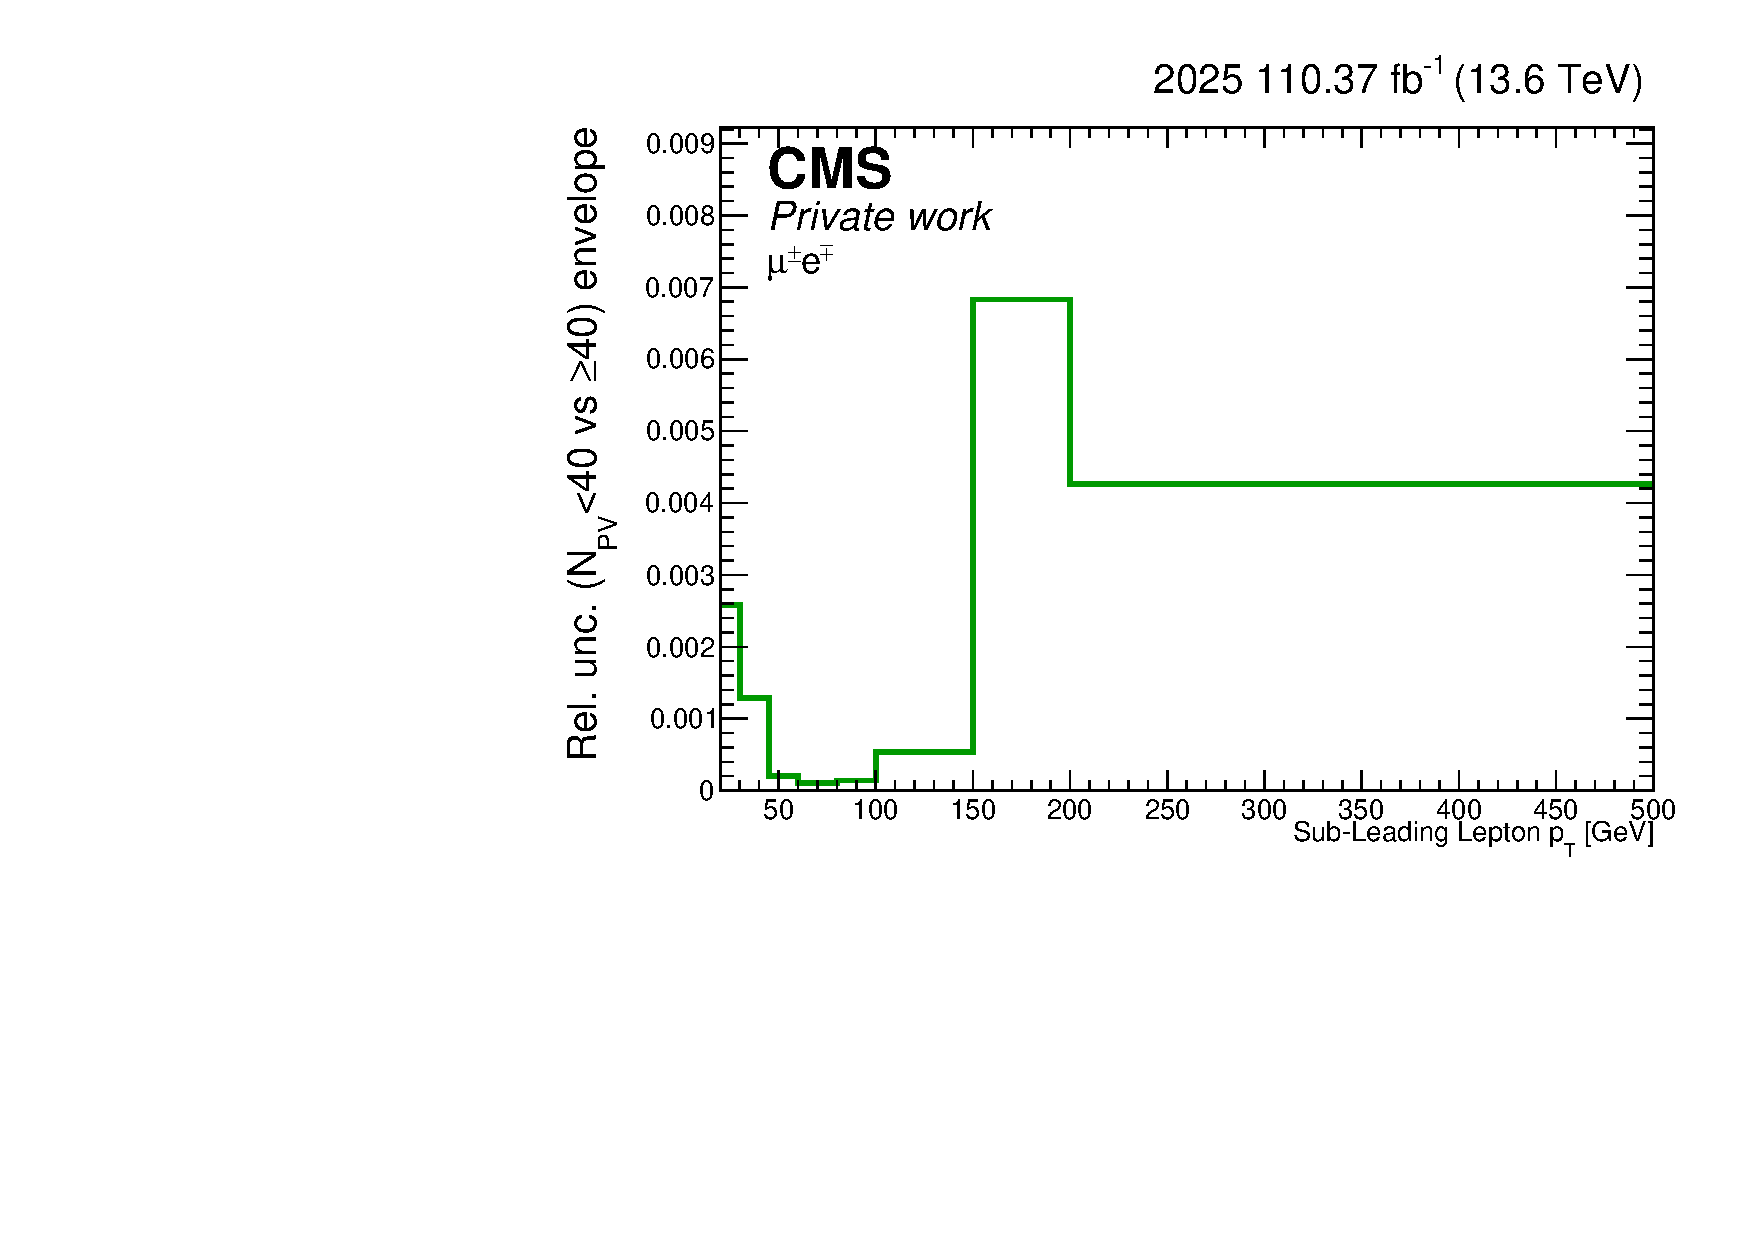
\includegraphics[width=0.48\linewidth]{figures/2025/MuEl/PV_Topology_Uncertainty/TopoPVUnc_Lep2pt.pdf}
\caption{PV Topology Uncertainty diagnostics in the $e\mu$ channel versus leading and subleading lepton momentum. Curves are reproduced with the production definitions; their exact numerical prescription requires confirmation.}\label{fig:study-MuEl-TopoPVUnc-2025}
\end{figure}
\begin{figure}[htbp]\centering
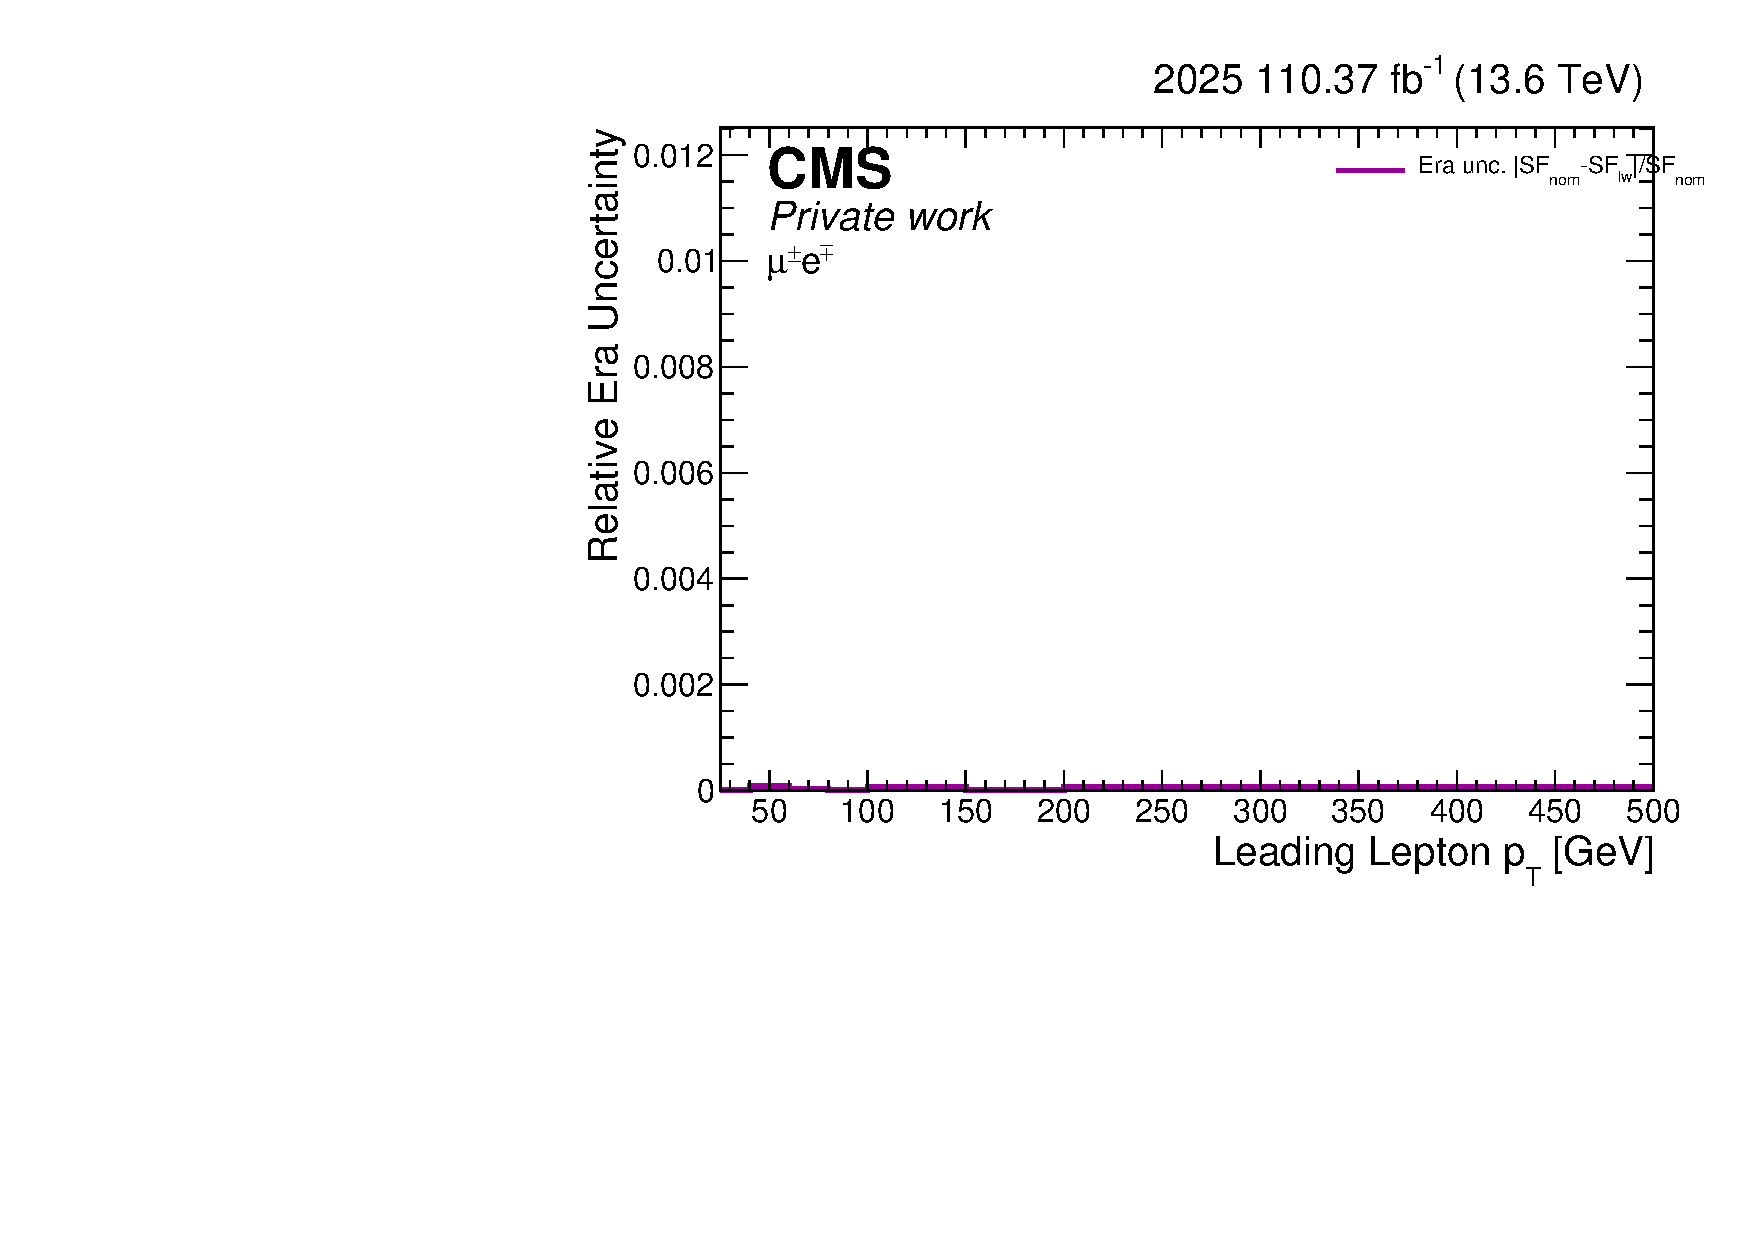
\includegraphics[width=0.48\linewidth]{figures/2025/MuEl/Era_Uncertainty/EraUnc_Lep1pt.pdf}
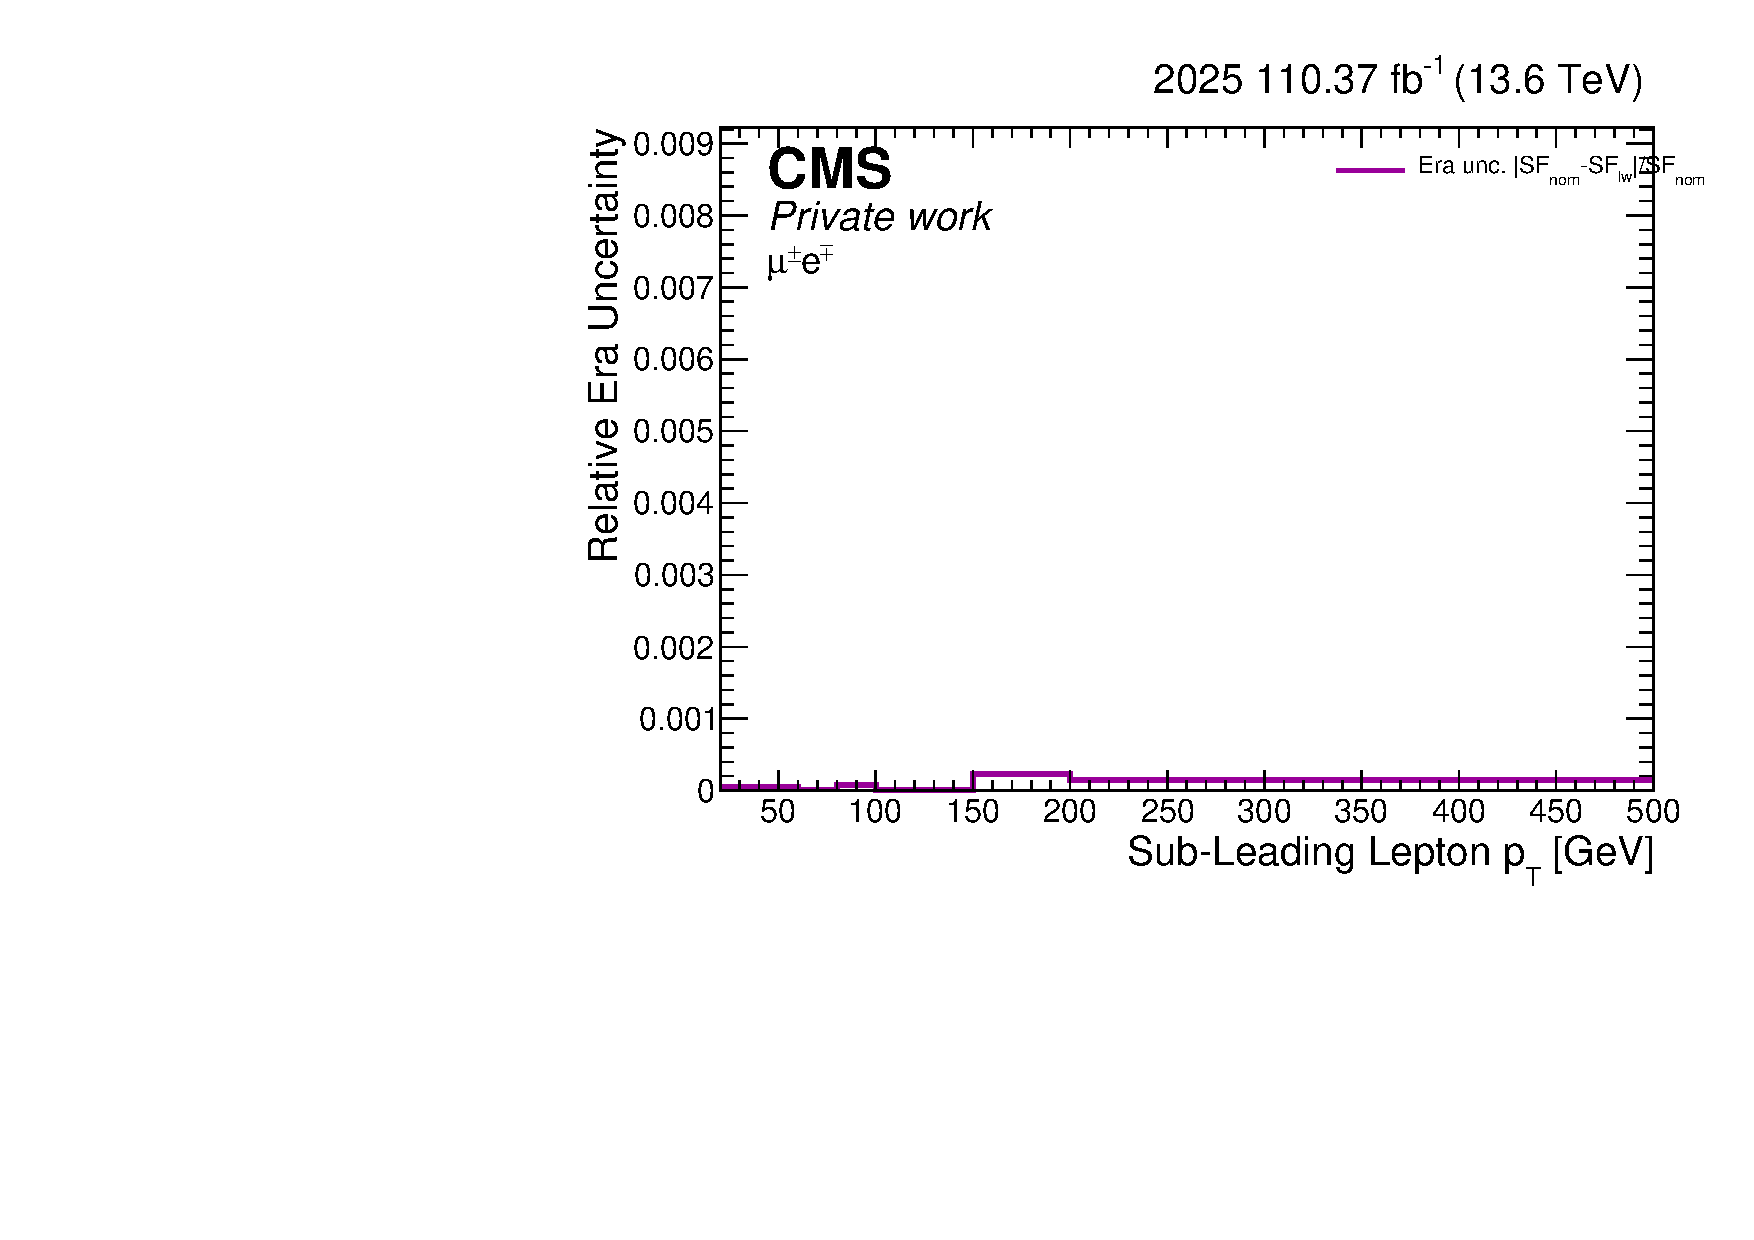
\includegraphics[width=0.48\linewidth]{figures/2025/MuEl/Era_Uncertainty/EraUnc_Lep2pt.pdf}
\caption{Era Uncertainty diagnostics in the $e\mu$ channel versus leading and subleading lepton momentum. Curves are reproduced with the production definitions; their exact numerical prescription requires confirmation.}\label{fig:study-MuEl-EraUnc-2025}
\end{figure}
\begin{figure}[htbp]\centering
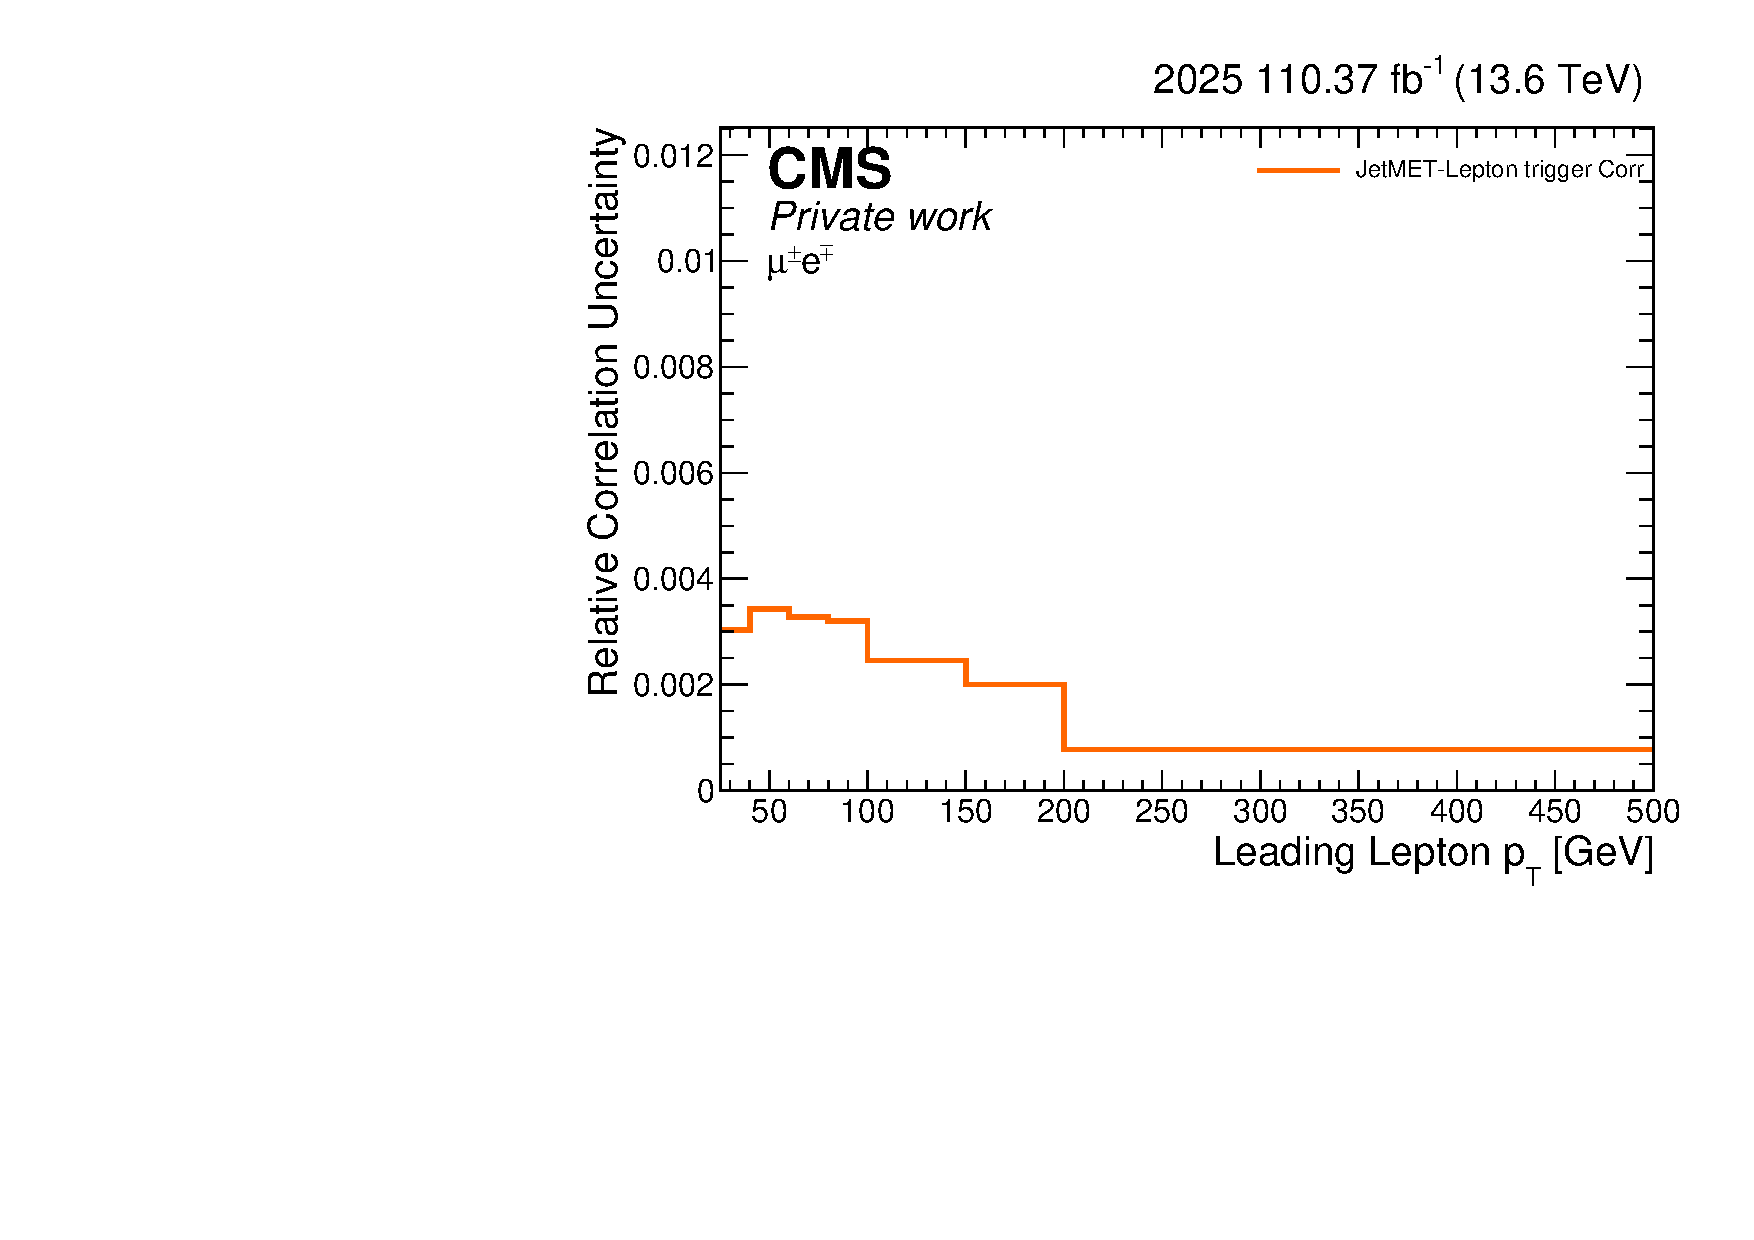
\includegraphics[width=0.48\linewidth]{figures/2025/MuEl/Correlation_Uncertainty/CorrUnc_Lep1pt.pdf}
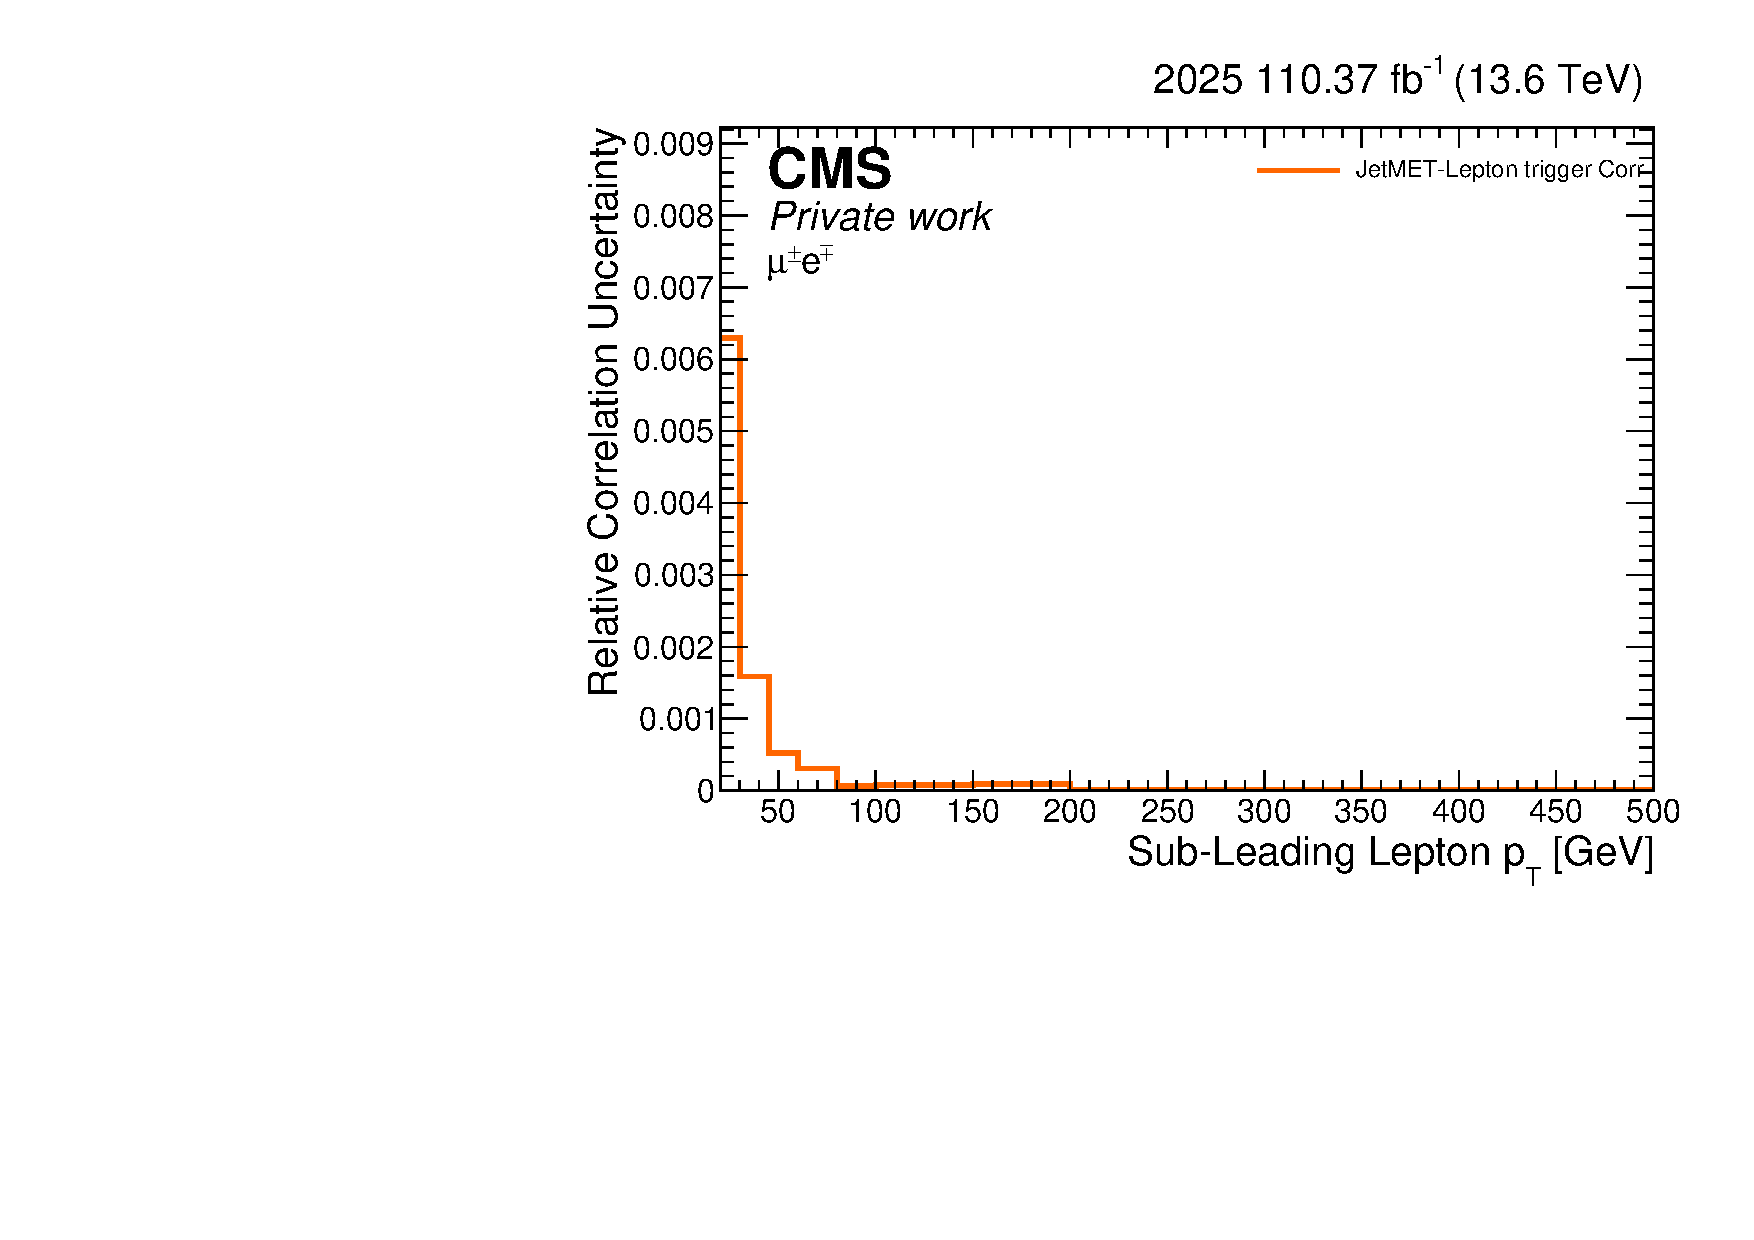
\includegraphics[width=0.48\linewidth]{figures/2025/MuEl/Correlation_Uncertainty/CorrUnc_Lep2pt.pdf}
\caption{Correlation Uncertainty diagnostics in the $e\mu$ channel versus leading and subleading lepton momentum. Curves are reproduced with the production definitions; their exact numerical prescription requires confirmation.}\label{fig:study-MuEl-CorrUnc-2025}
\end{figure}
\begin{figure}[htbp]\centering
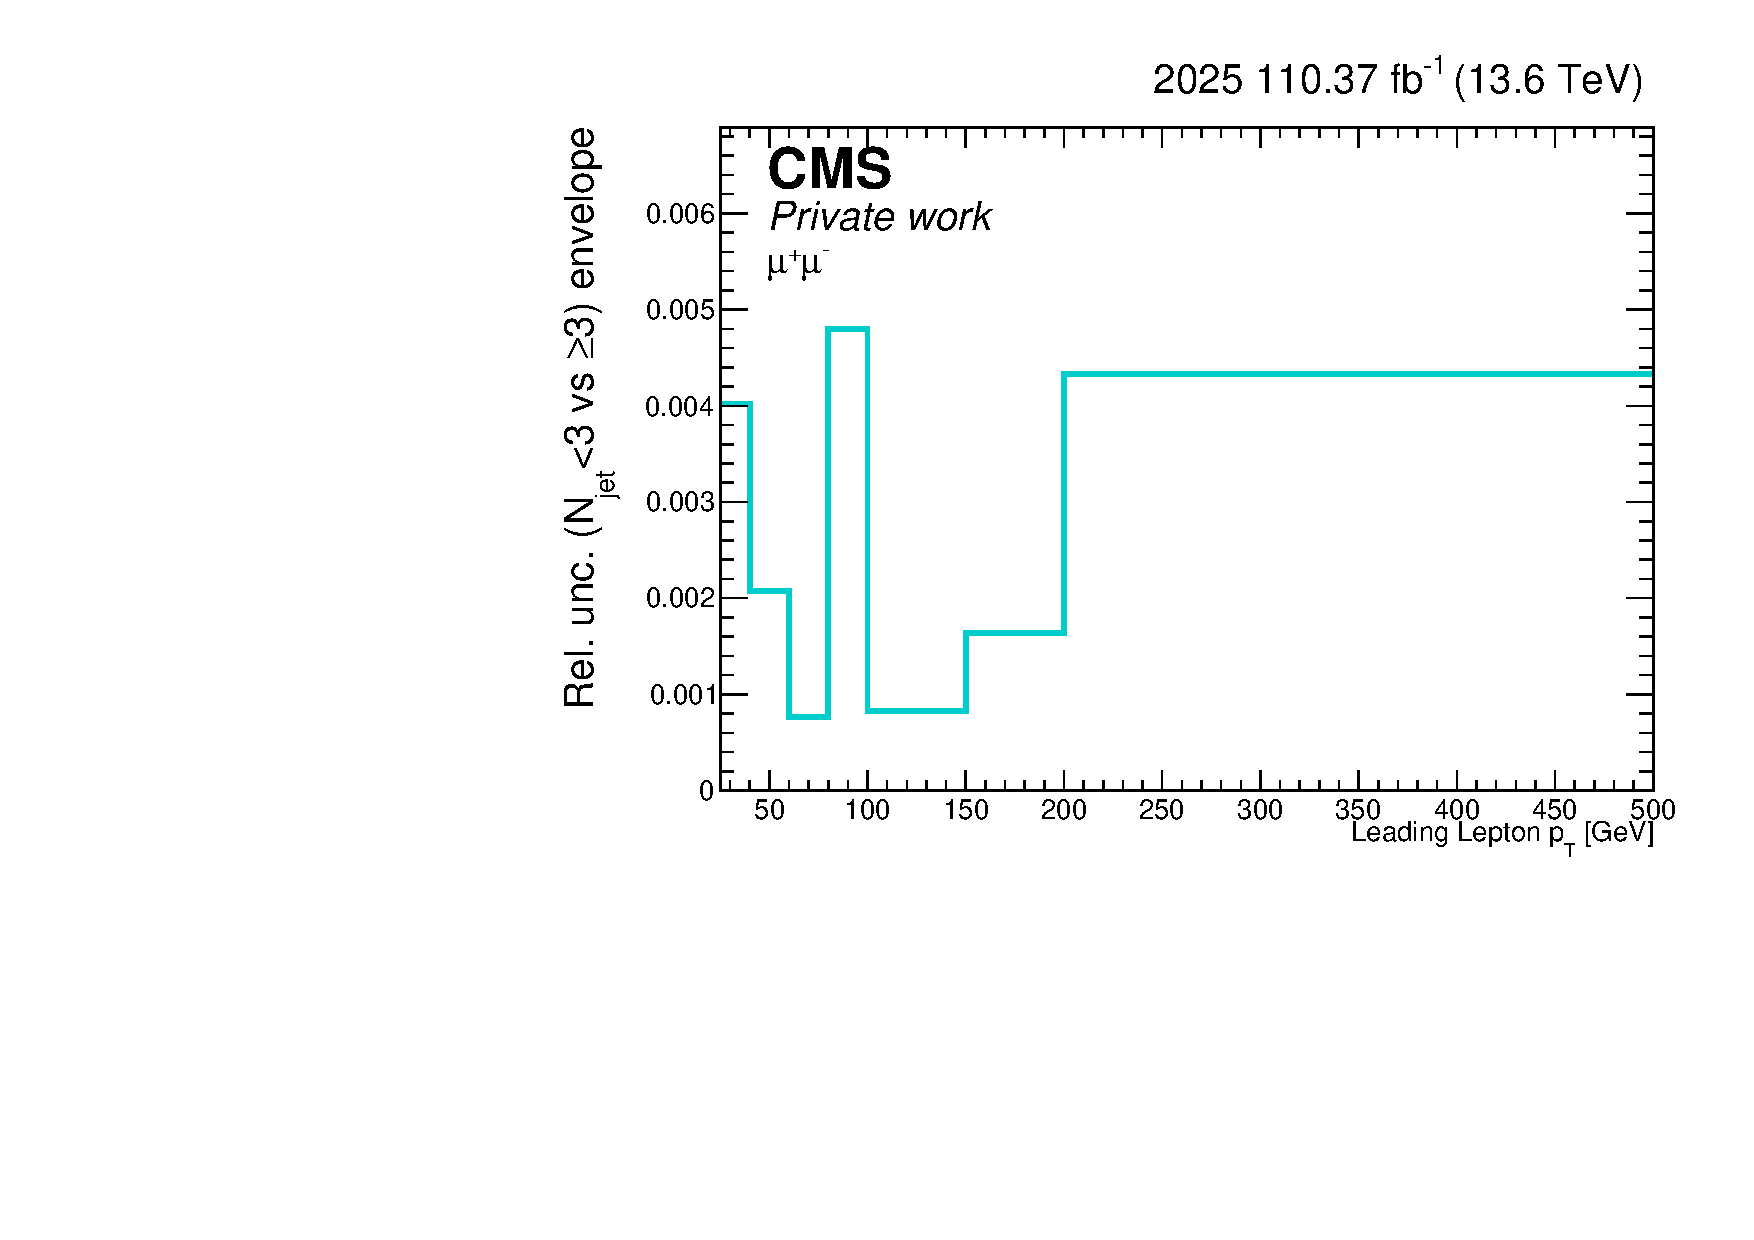
\includegraphics[width=0.48\linewidth]{figures/2025/MuMu/Jet_Topology_Uncertainty/TopoJetUnc_Lep1pt.pdf}
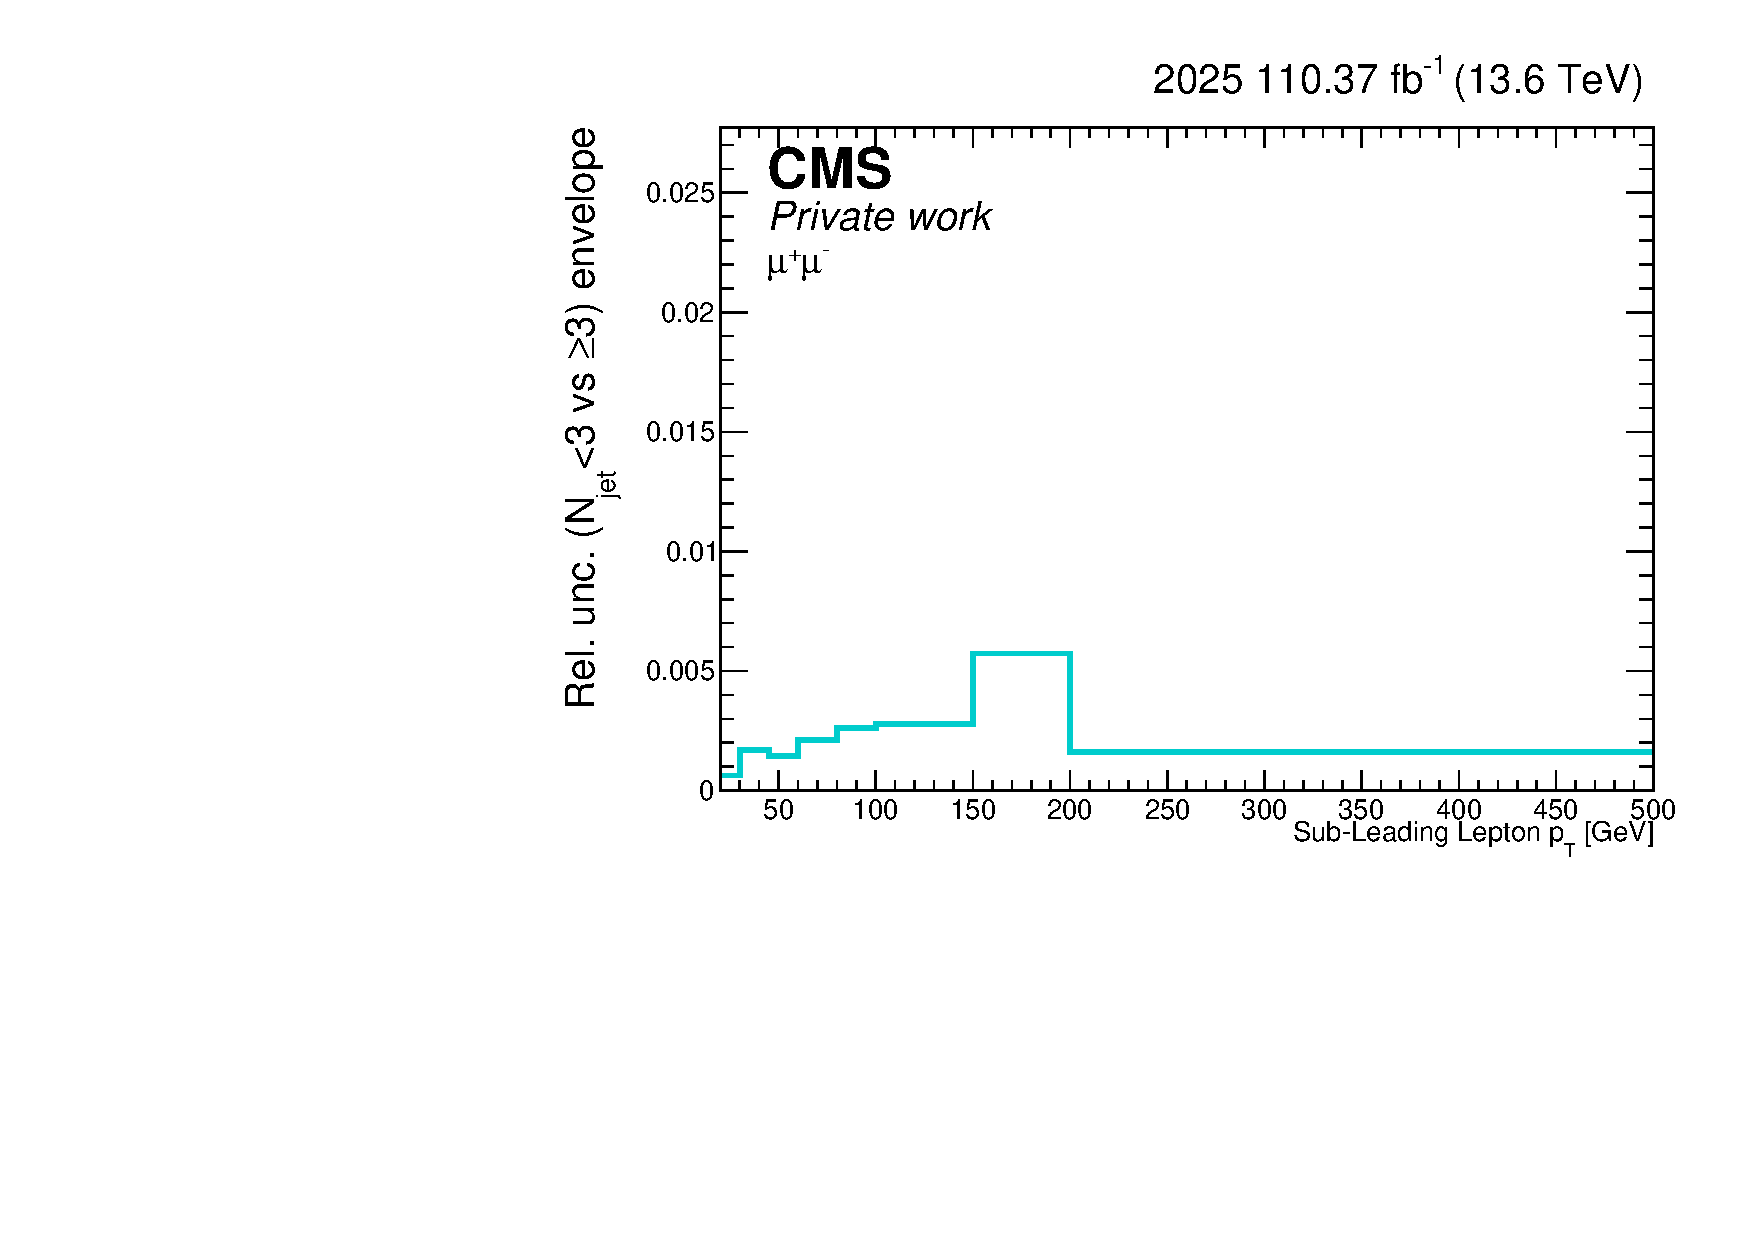
\includegraphics[width=0.48\linewidth]{figures/2025/MuMu/Jet_Topology_Uncertainty/TopoJetUnc_Lep2pt.pdf}
\caption{Jet Topology Uncertainty diagnostics in the $\mu\mu$ channel versus leading and subleading lepton momentum. Curves are reproduced with the production definitions; their exact numerical prescription requires confirmation.}\label{fig:study-MuMu-TopoJetUnc-2025}
\end{figure}
\begin{figure}[htbp]\centering
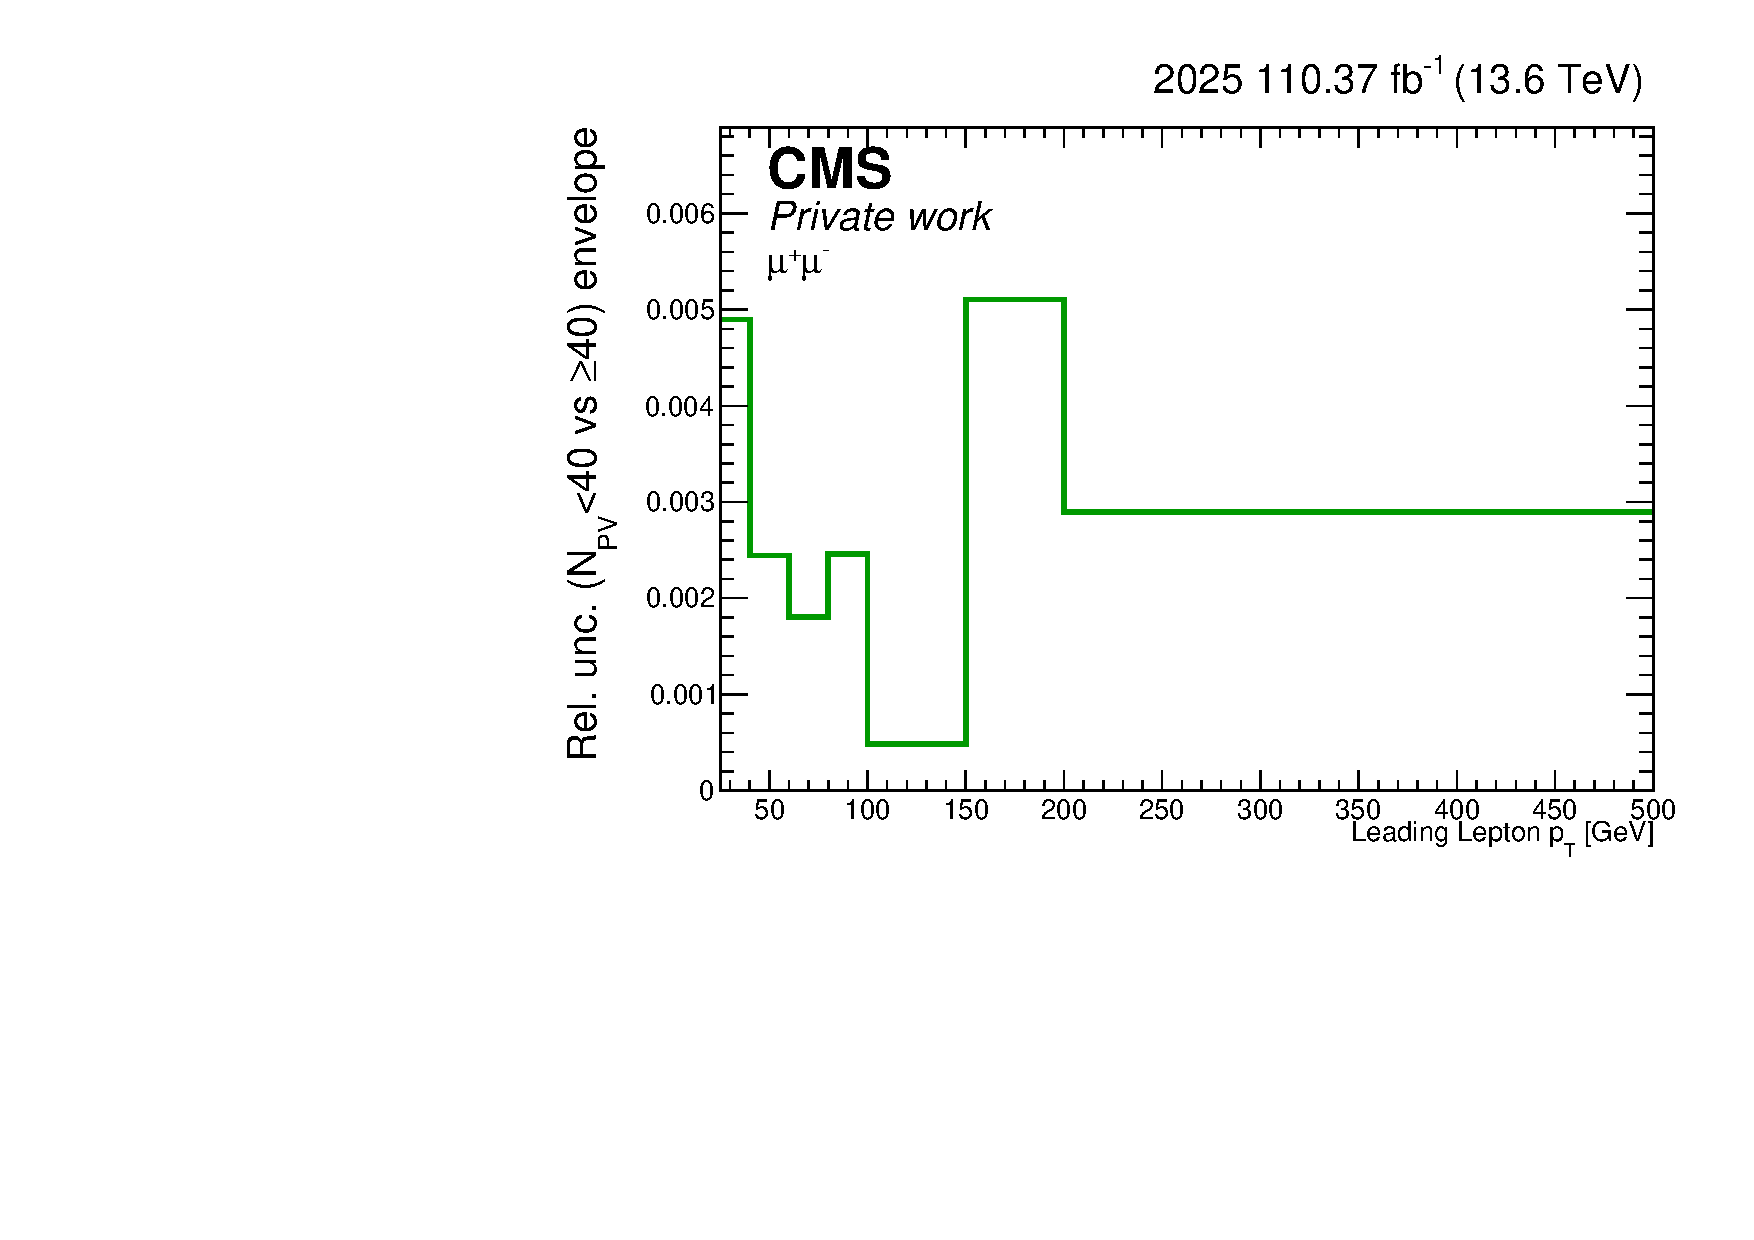
\includegraphics[width=0.48\linewidth]{figures/2025/MuMu/PV_Topology_Uncertainty/TopoPVUnc_Lep1pt.pdf}
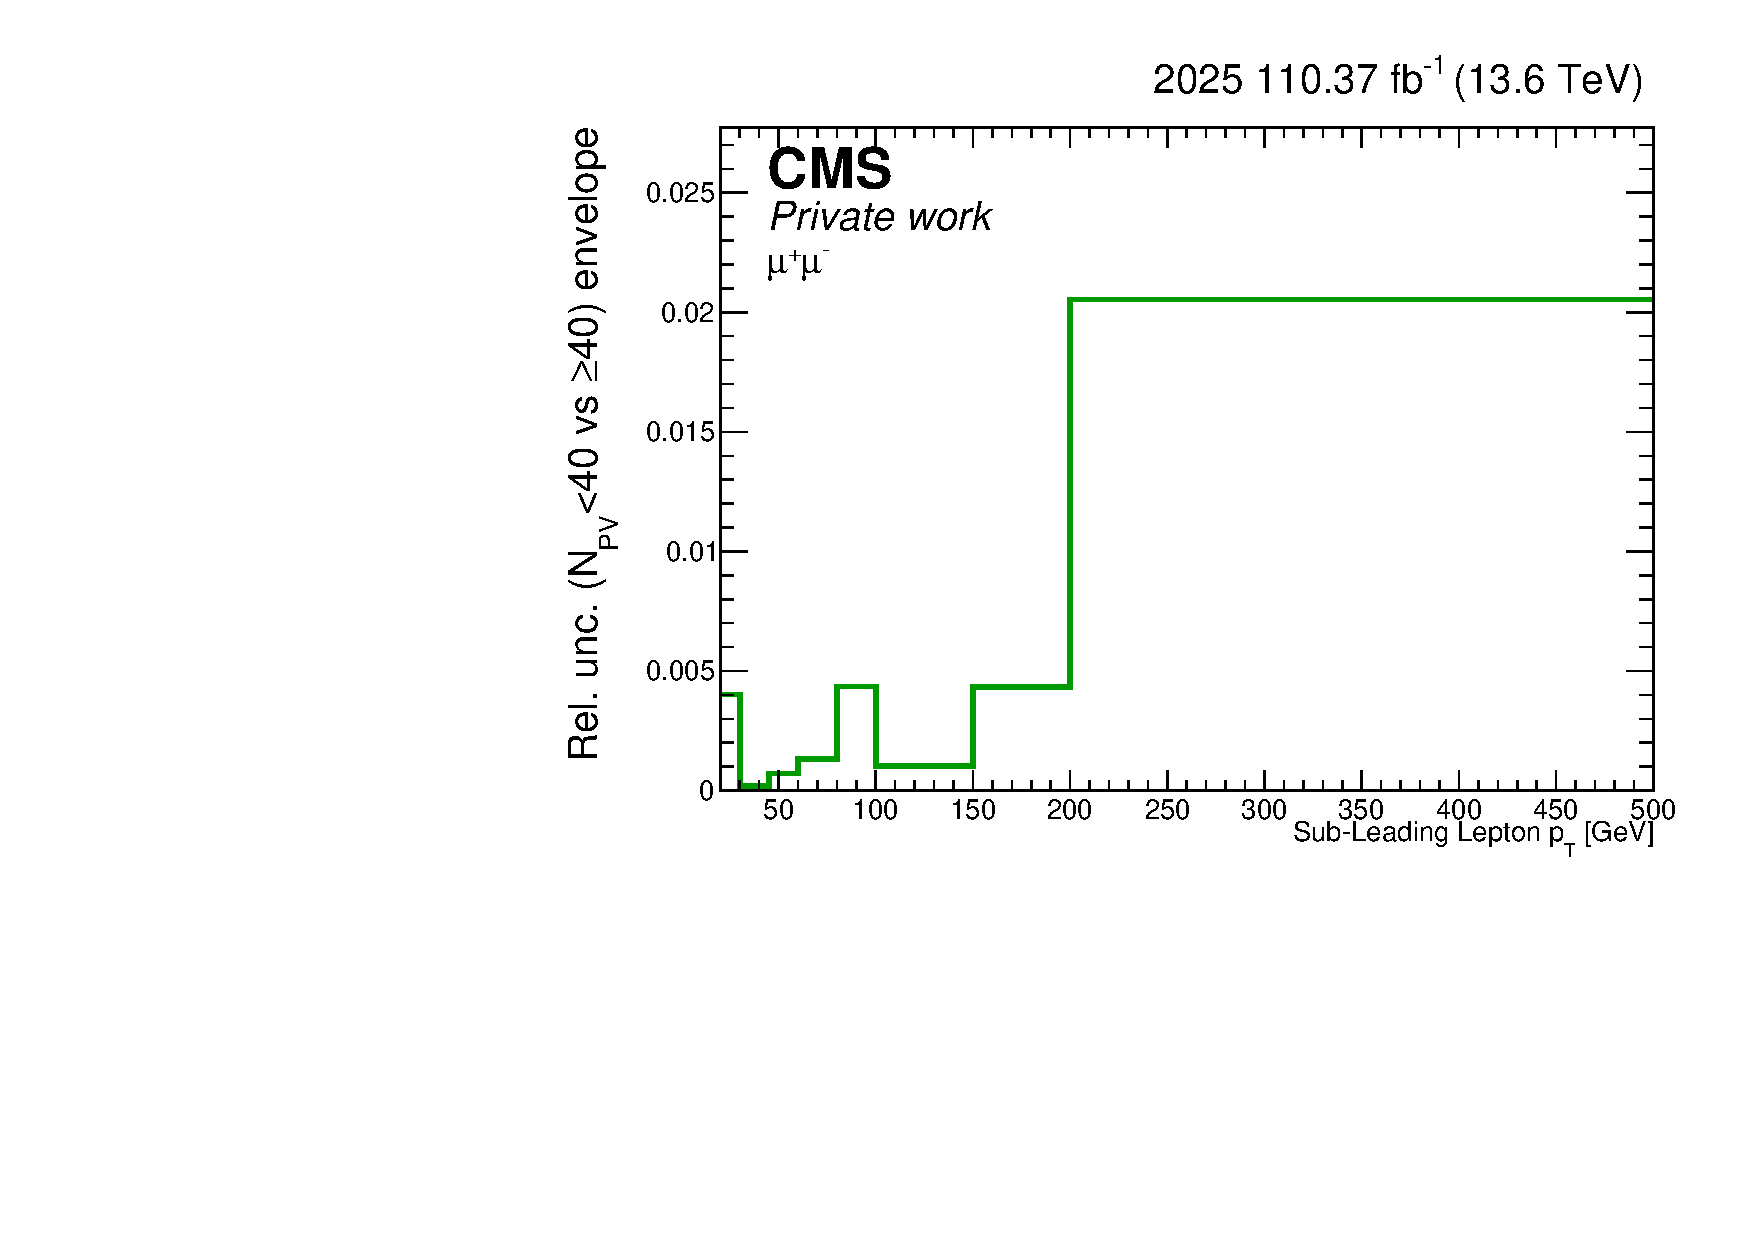
\includegraphics[width=0.48\linewidth]{figures/2025/MuMu/PV_Topology_Uncertainty/TopoPVUnc_Lep2pt.pdf}
\caption{PV Topology Uncertainty diagnostics in the $\mu\mu$ channel versus leading and subleading lepton momentum. Curves are reproduced with the production definitions; their exact numerical prescription requires confirmation.}\label{fig:study-MuMu-TopoPVUnc-2025}
\end{figure}
\begin{figure}[htbp]\centering
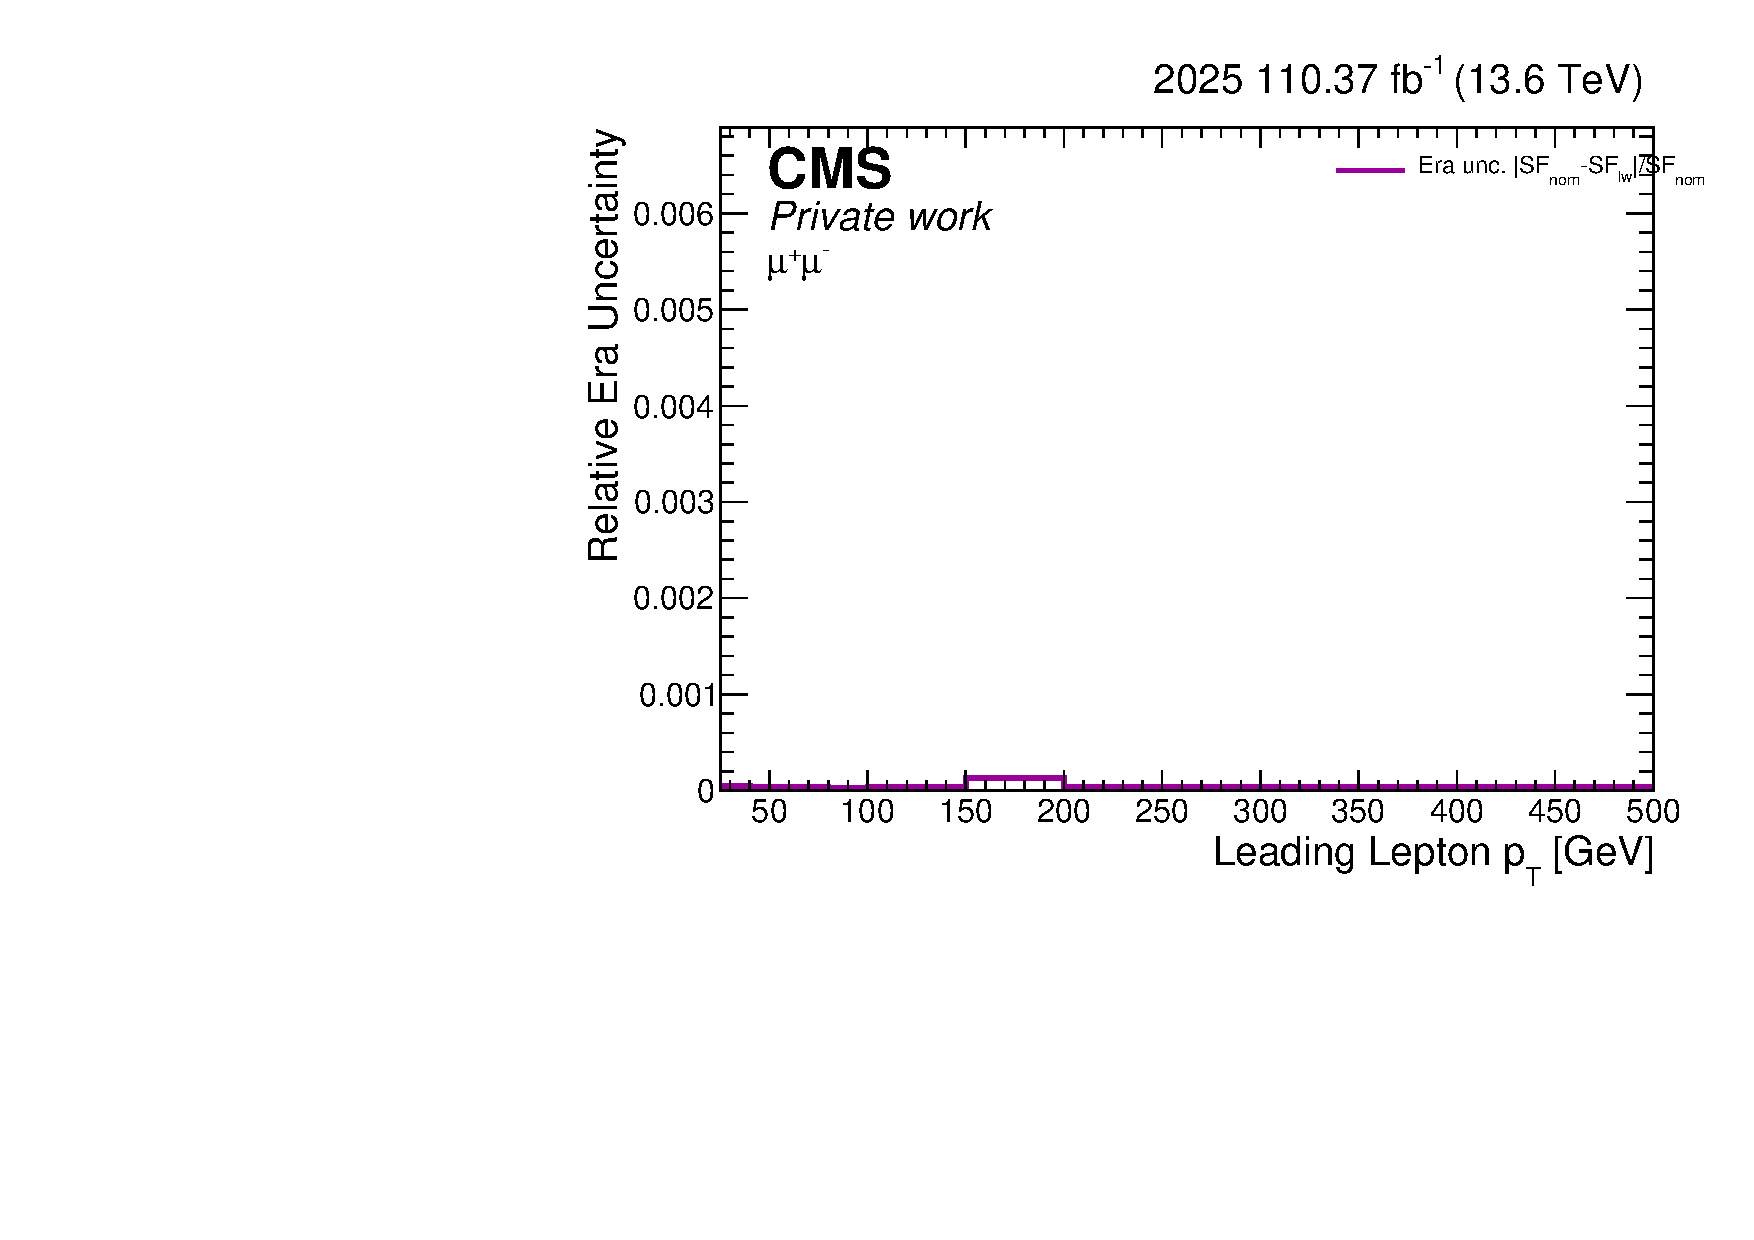
\includegraphics[width=0.48\linewidth]{figures/2025/MuMu/Era_Uncertainty/EraUnc_Lep1pt.pdf}
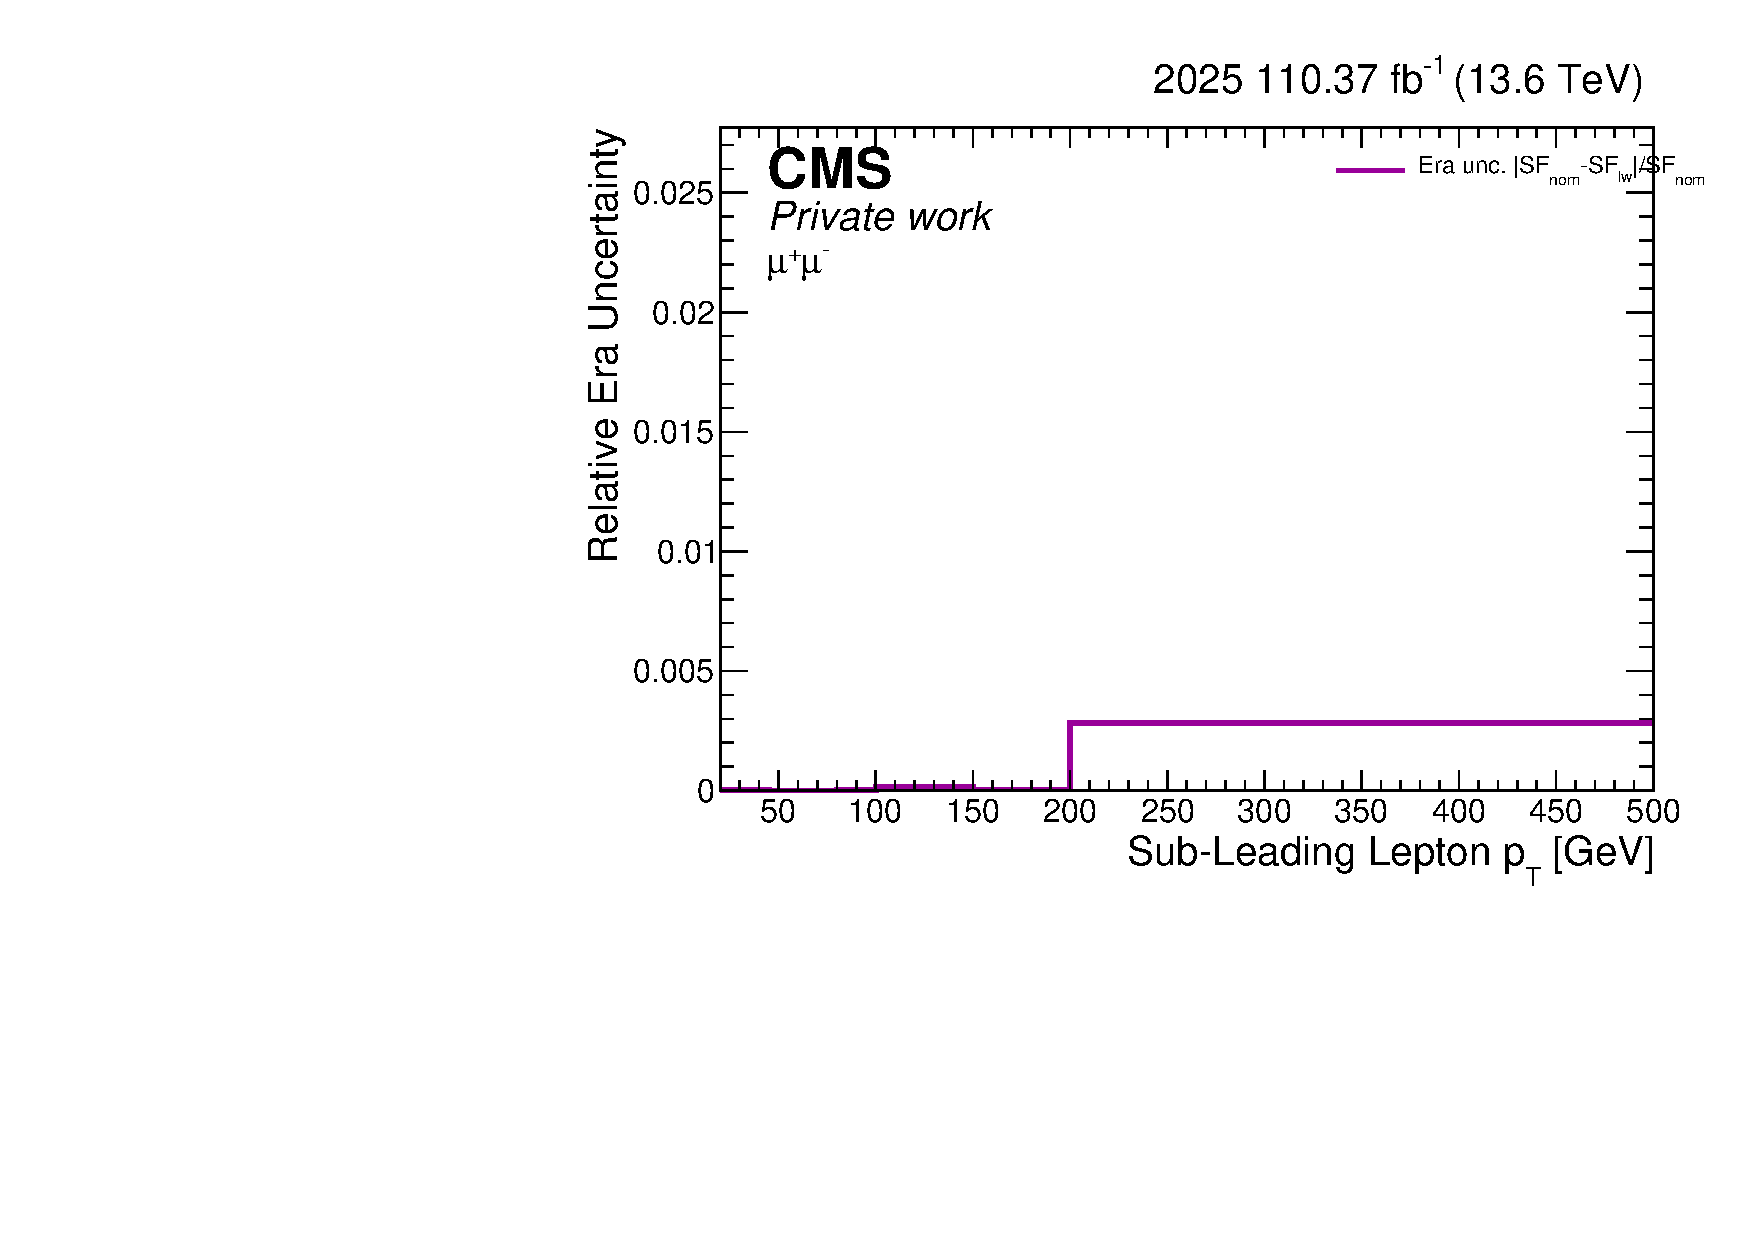
\includegraphics[width=0.48\linewidth]{figures/2025/MuMu/Era_Uncertainty/EraUnc_Lep2pt.pdf}
\caption{Era Uncertainty diagnostics in the $\mu\mu$ channel versus leading and subleading lepton momentum. Curves are reproduced with the production definitions; their exact numerical prescription requires confirmation.}\label{fig:study-MuMu-EraUnc-2025}
\end{figure}
\begin{figure}[htbp]\centering
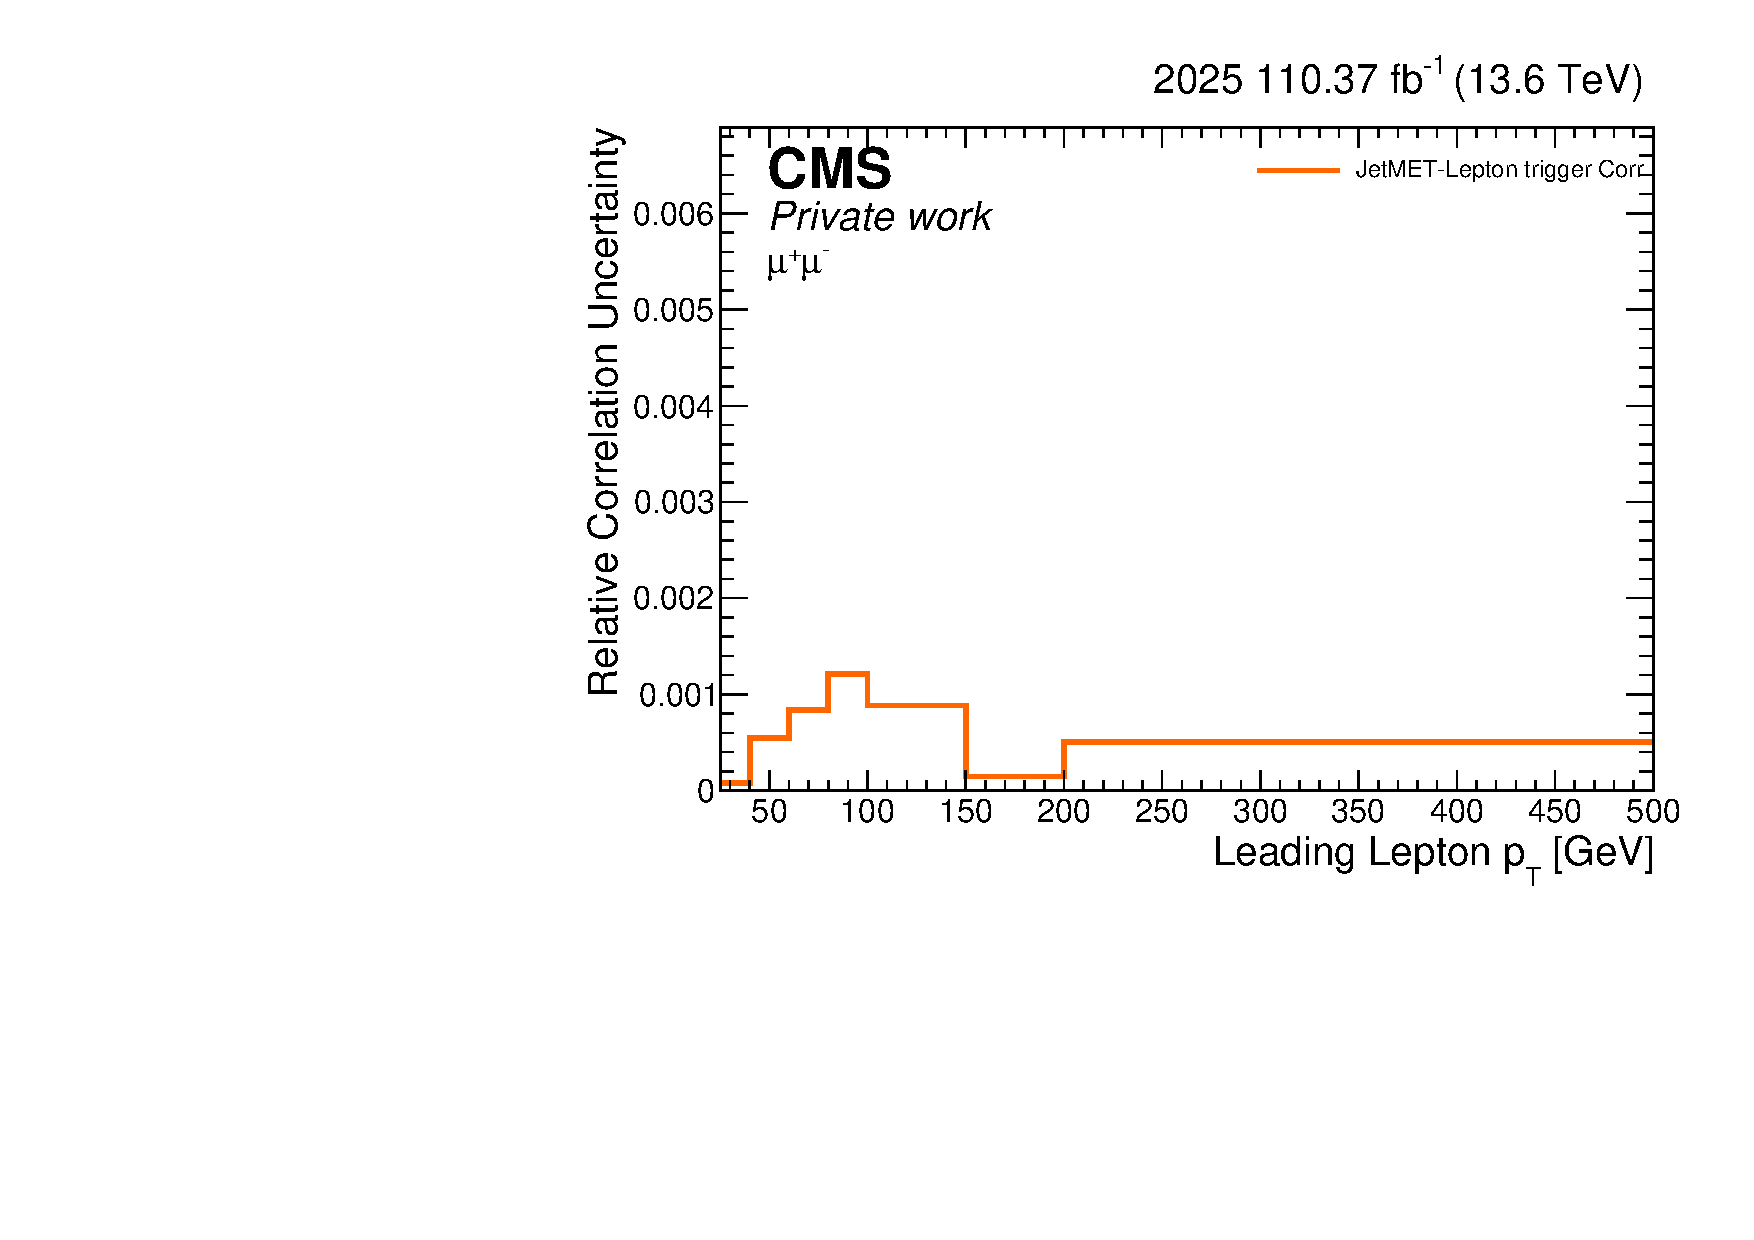
\includegraphics[width=0.48\linewidth]{figures/2025/MuMu/Correlation_Uncertainty/CorrUnc_Lep1pt.pdf}
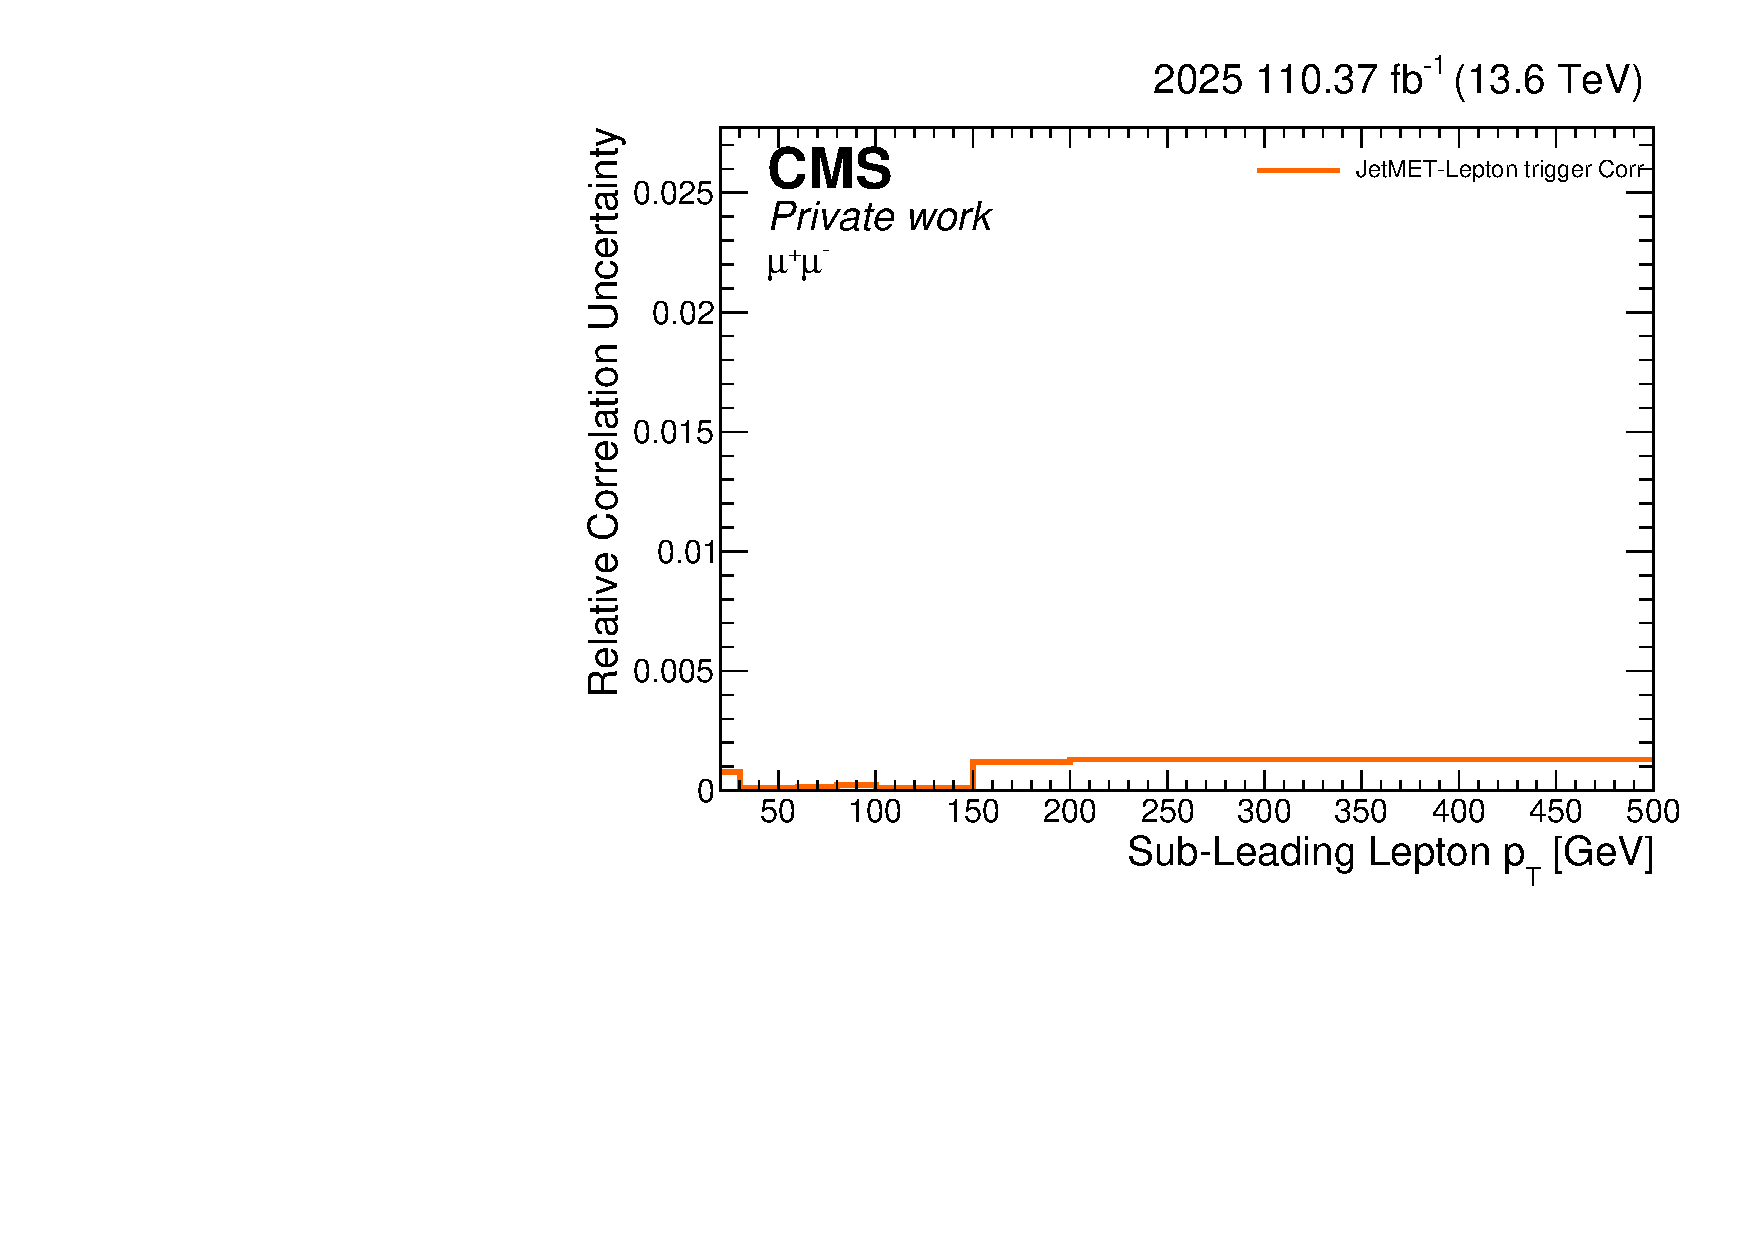
\includegraphics[width=0.48\linewidth]{figures/2025/MuMu/Correlation_Uncertainty/CorrUnc_Lep2pt.pdf}
\caption{Correlation Uncertainty diagnostics in the $\mu\mu$ channel versus leading and subleading lepton momentum. Curves are reproduced with the production definitions; their exact numerical prescription requires confirmation.}\label{fig:study-MuMu-CorrUnc-2025}
\end{figure}



\clearpage\section{Selected 2025 supporting distributions}\label{app:2025-support-2025}
The following distributions document the efficiency inputs, statistical precision, and uncertainty composition for the 2025 measurement. Only inclusive distributions directly related to the correction or its principal checks are selected. The jet- and vertex-split variants and the full set of individual-jet and angular distributions are not reproduced. These plots use the measurement sample and are not independent closure tests.
\subsection{$ee$ channel}
\begin{figure}[htbp]\centering
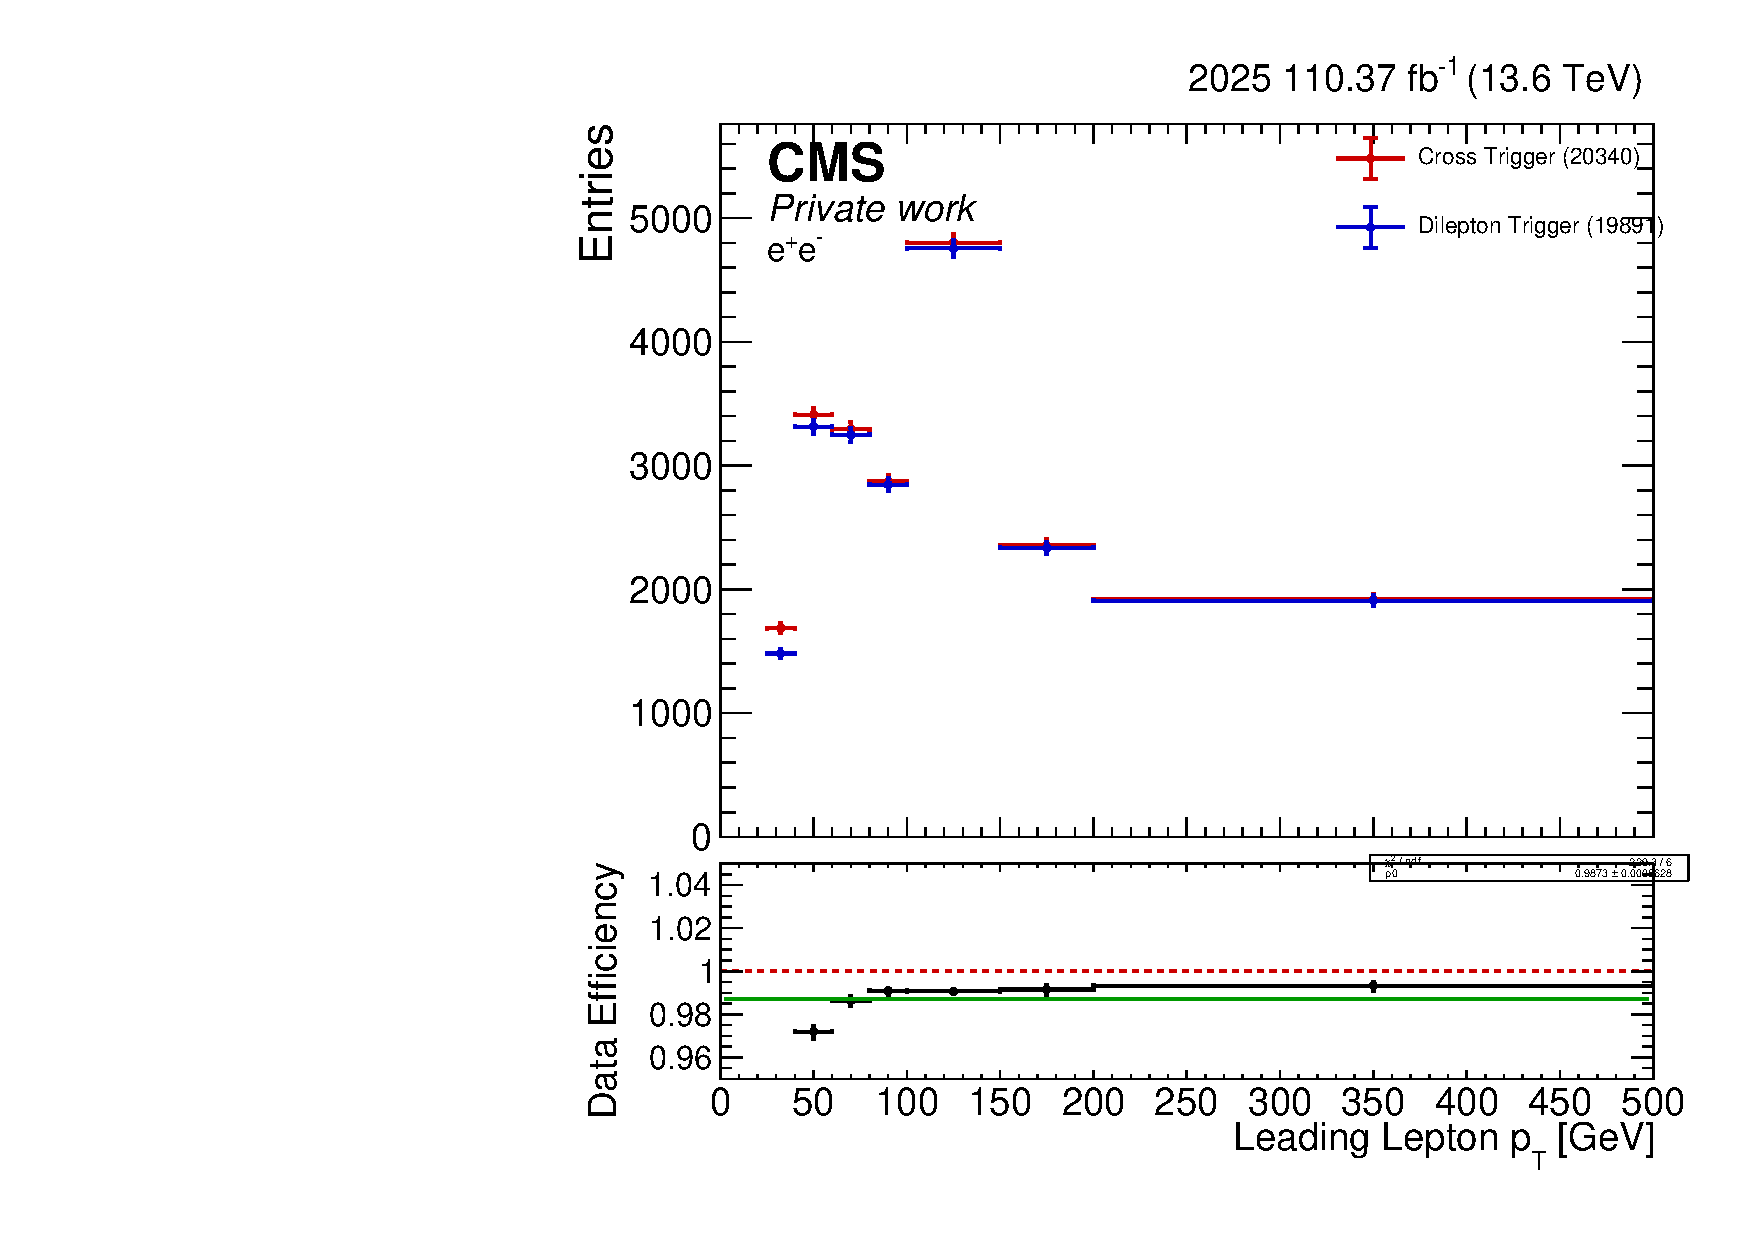
\includegraphics[width=0.48\linewidth]{figures/2025/ElEl/TrigEffData/TrigEff_Lep1pt.pdf}
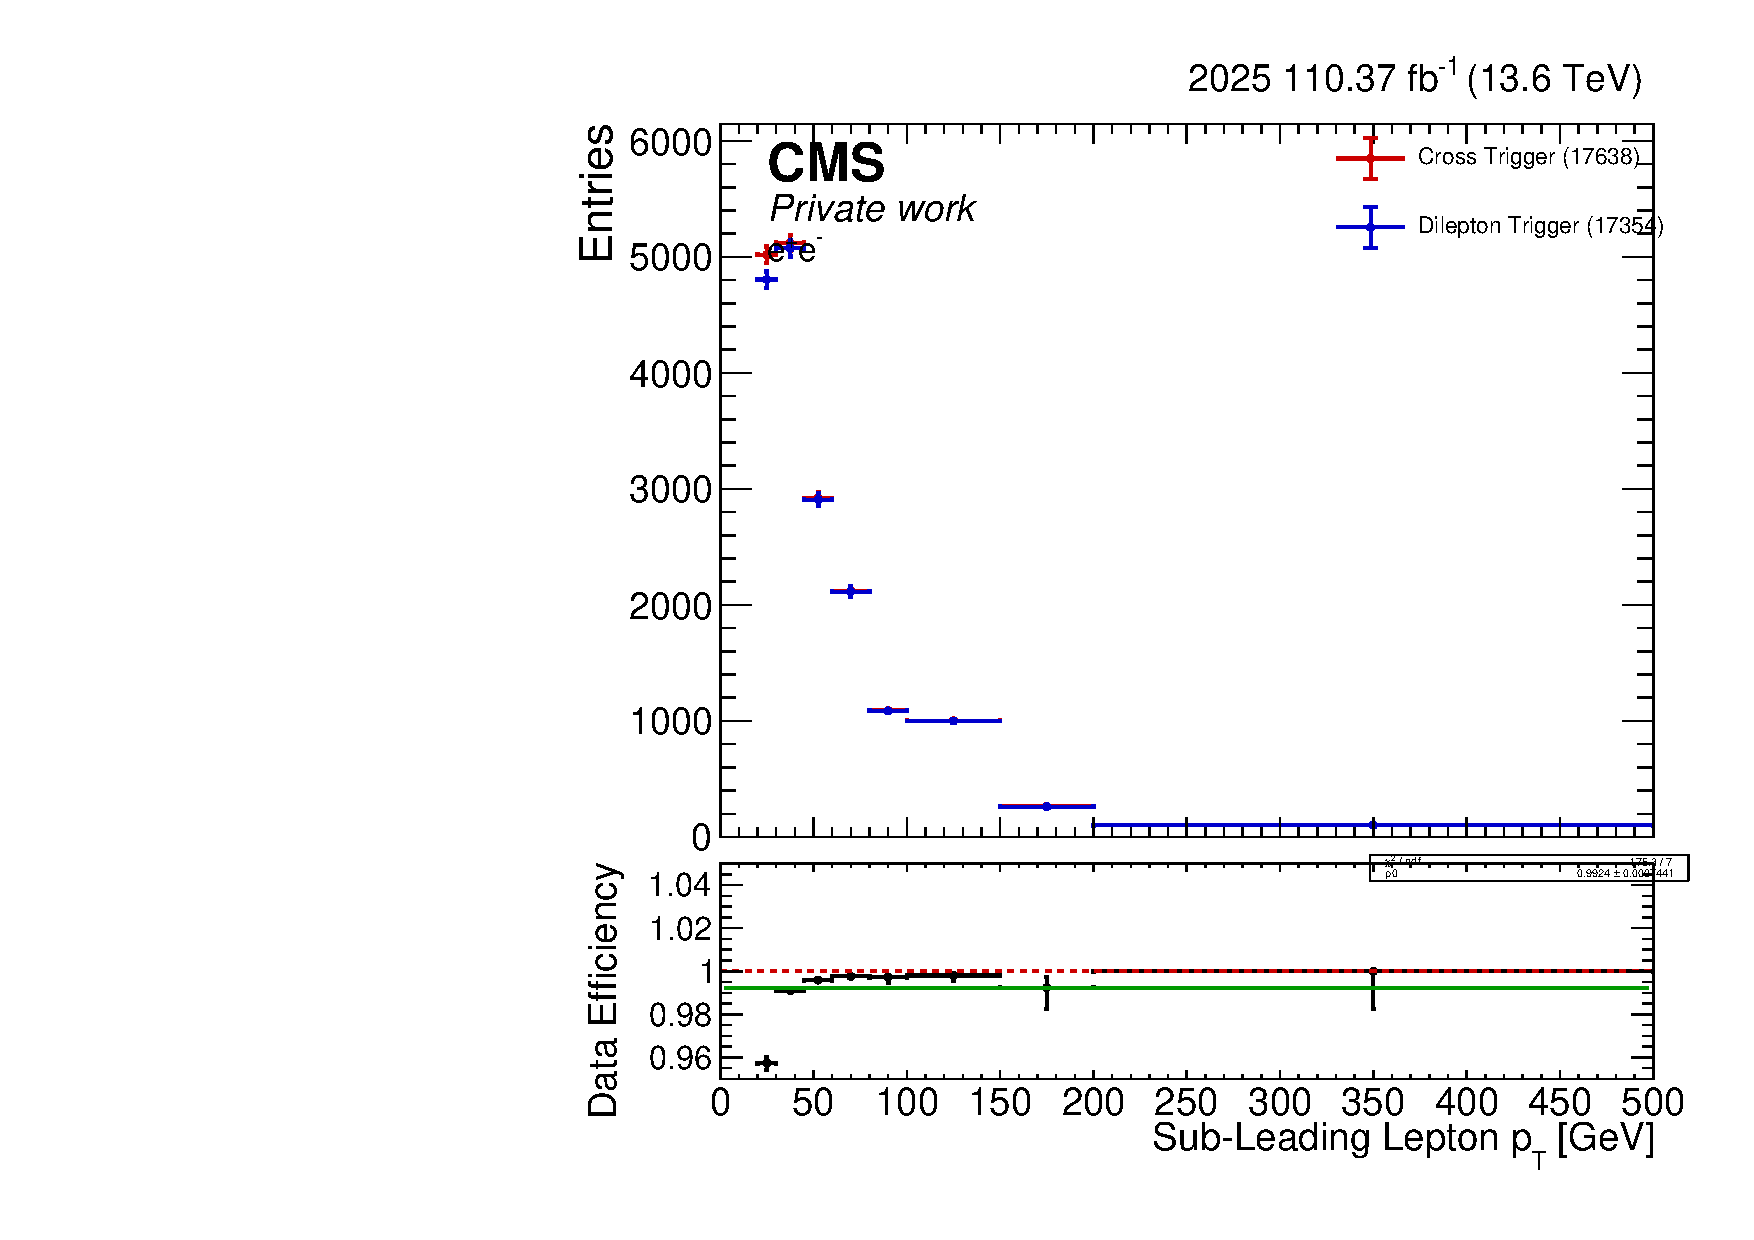
\includegraphics[width=0.48\linewidth]{figures/2025/ElEl/TrigEffData/TrigEff_Lep2pt.pdf}
\caption{Data trigger numerator and reference-sample distributions (upper panels), with their efficiency ratios (lower panels) in the $ee$ channel. Left and right: leading and subleading lepton $p_{\mathrm{T}}$.}\label{fig:extra-ElEl-TrigEffData-Lep1pt-2025}\end{figure}
\begin{figure}[p]\centering
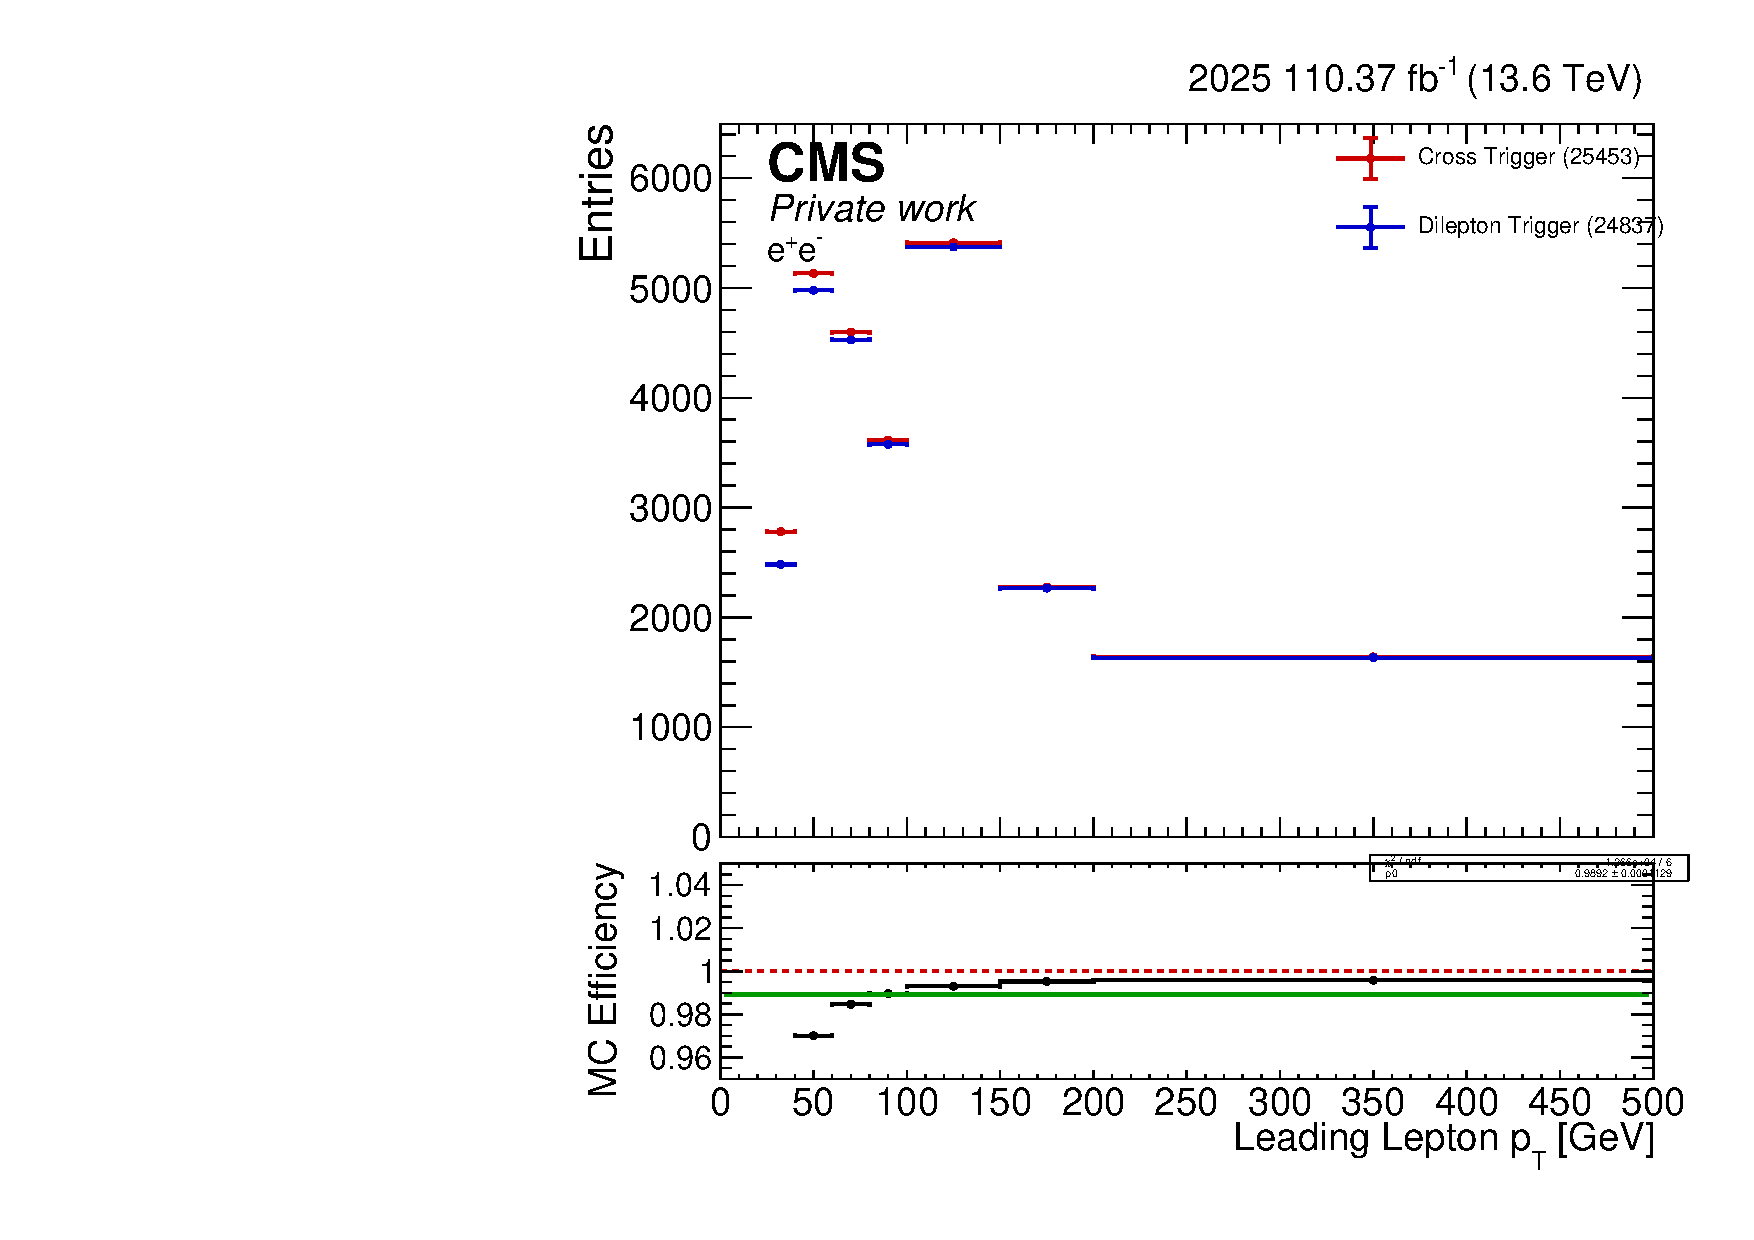
\includegraphics[width=0.48\linewidth]{figures/2025/ElEl/TrigEffMC/TrigEff_Lep1pt.pdf}
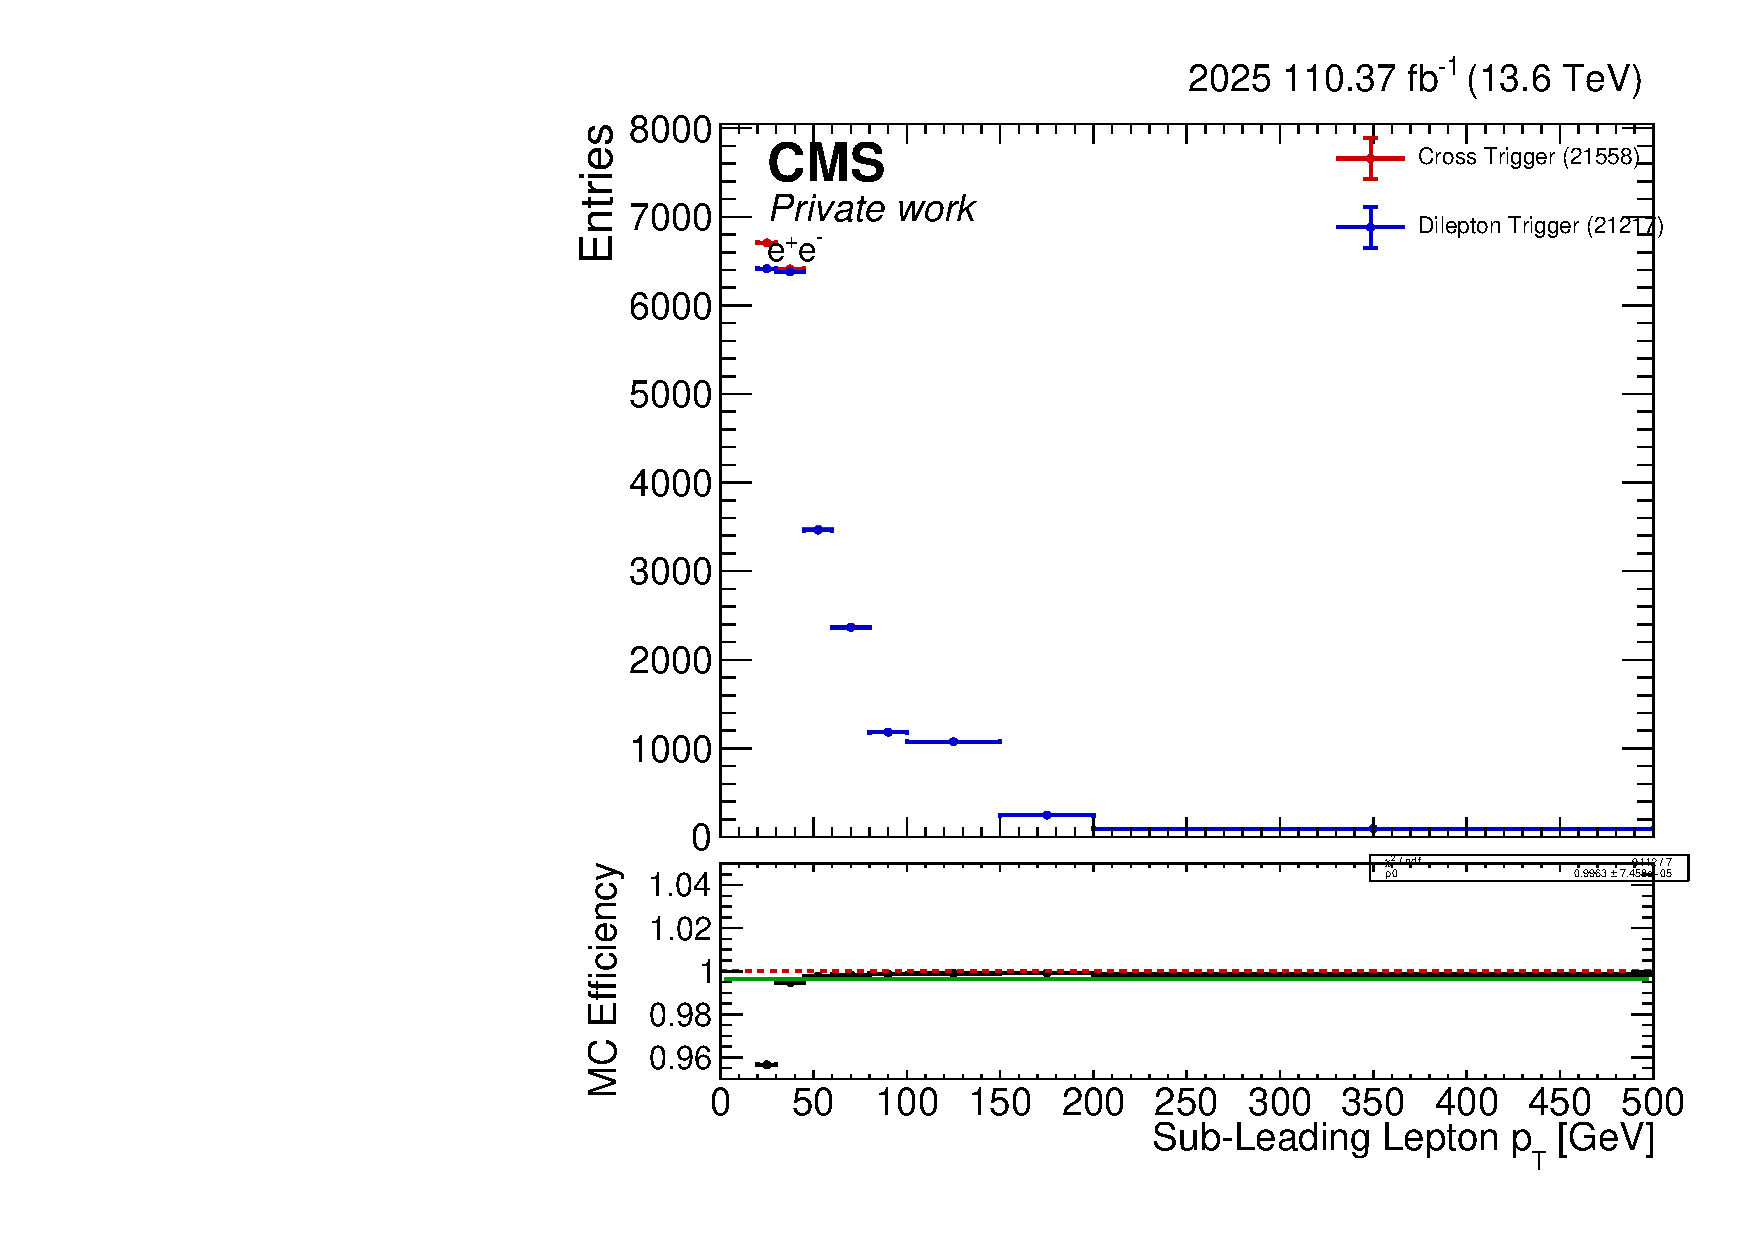
\includegraphics[width=0.48\linewidth]{figures/2025/ElEl/TrigEffMC/TrigEff_Lep2pt.pdf}
\caption{Simulated trigger numerator and reference-sample distributions (upper panels), with their efficiency ratios (lower panels) in the $ee$ channel. Left and right: leading and subleading lepton $p_{\mathrm{T}}$.}\label{fig:extra-ElEl-TrigEffMC-Lep1pt-2025}\end{figure}
\begin{figure}[p]\centering
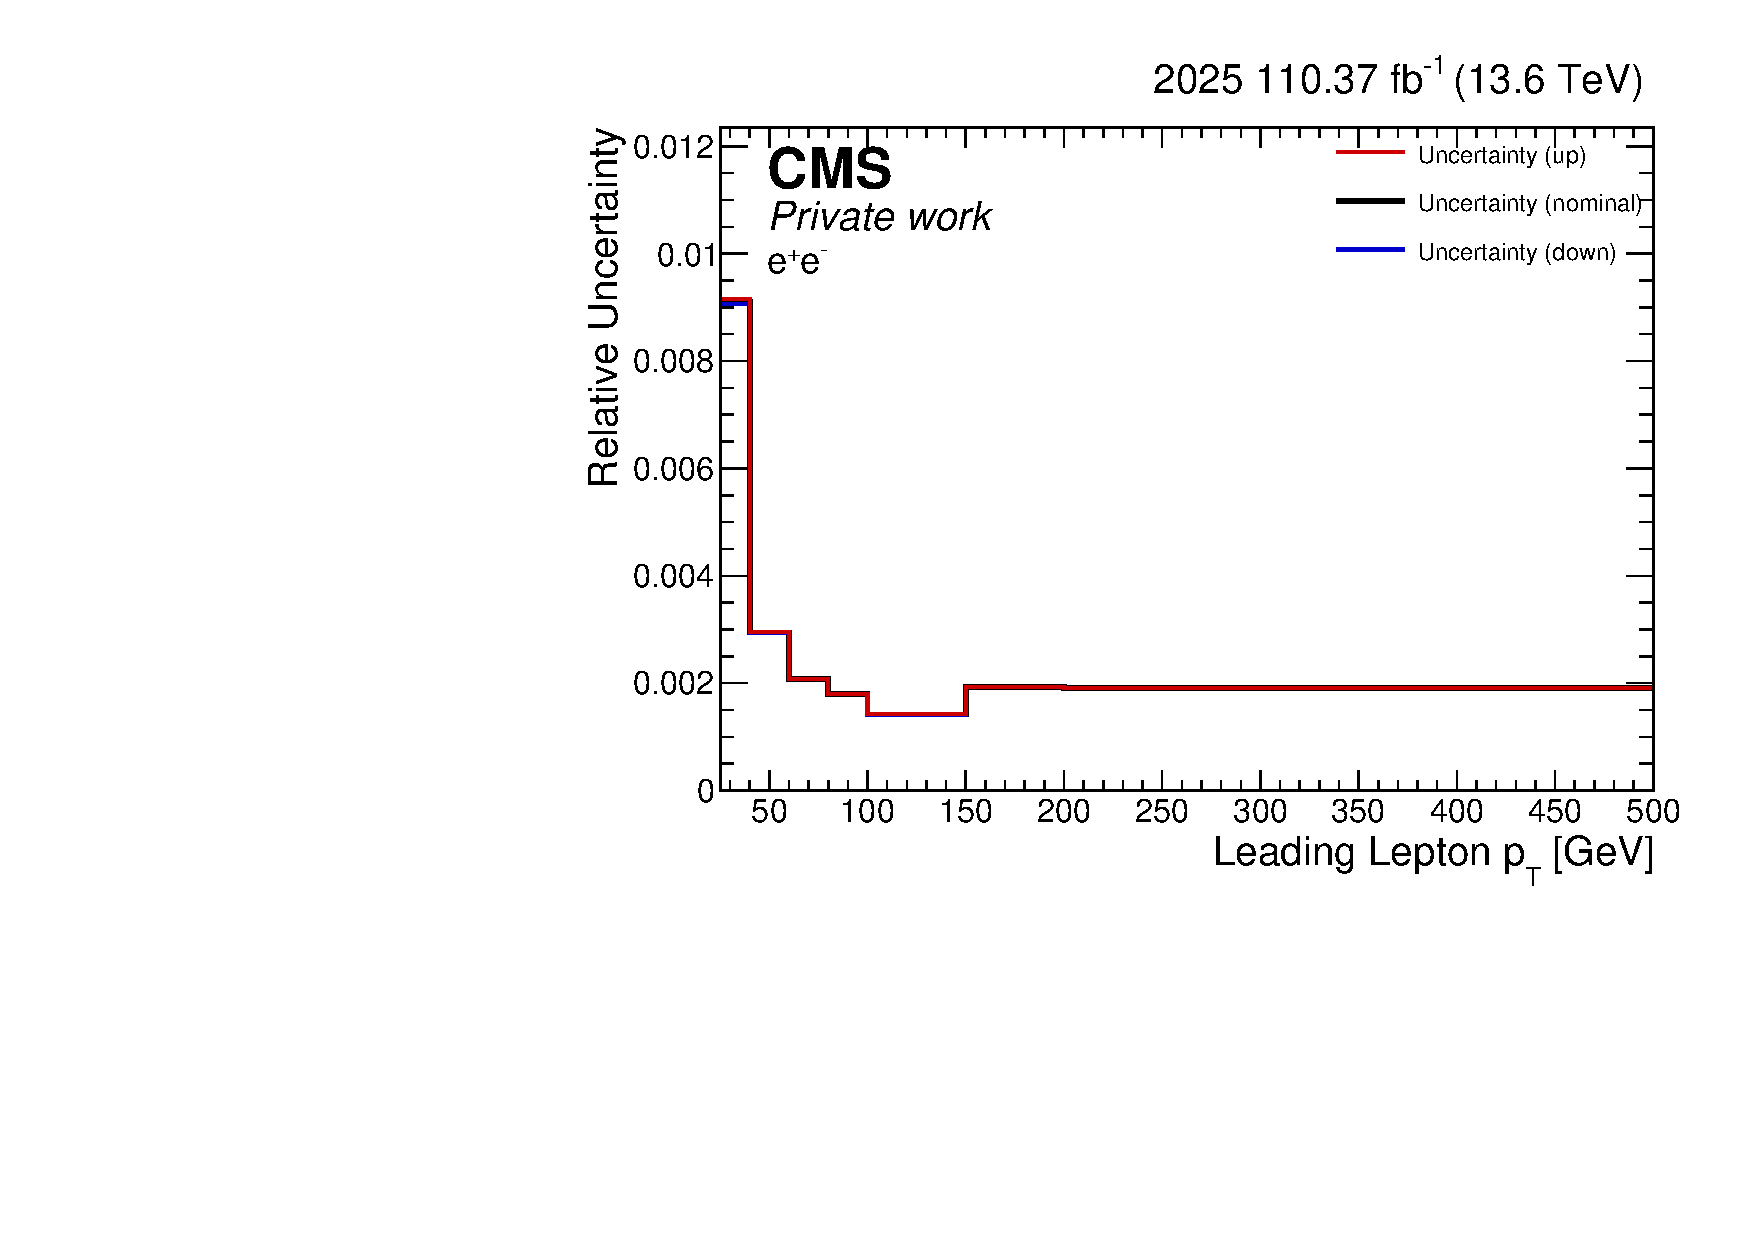
\includegraphics[width=0.48\linewidth]{figures/2025/ElEl/Statistical_Uncertainty/UncRatio_Lep1pt.pdf}
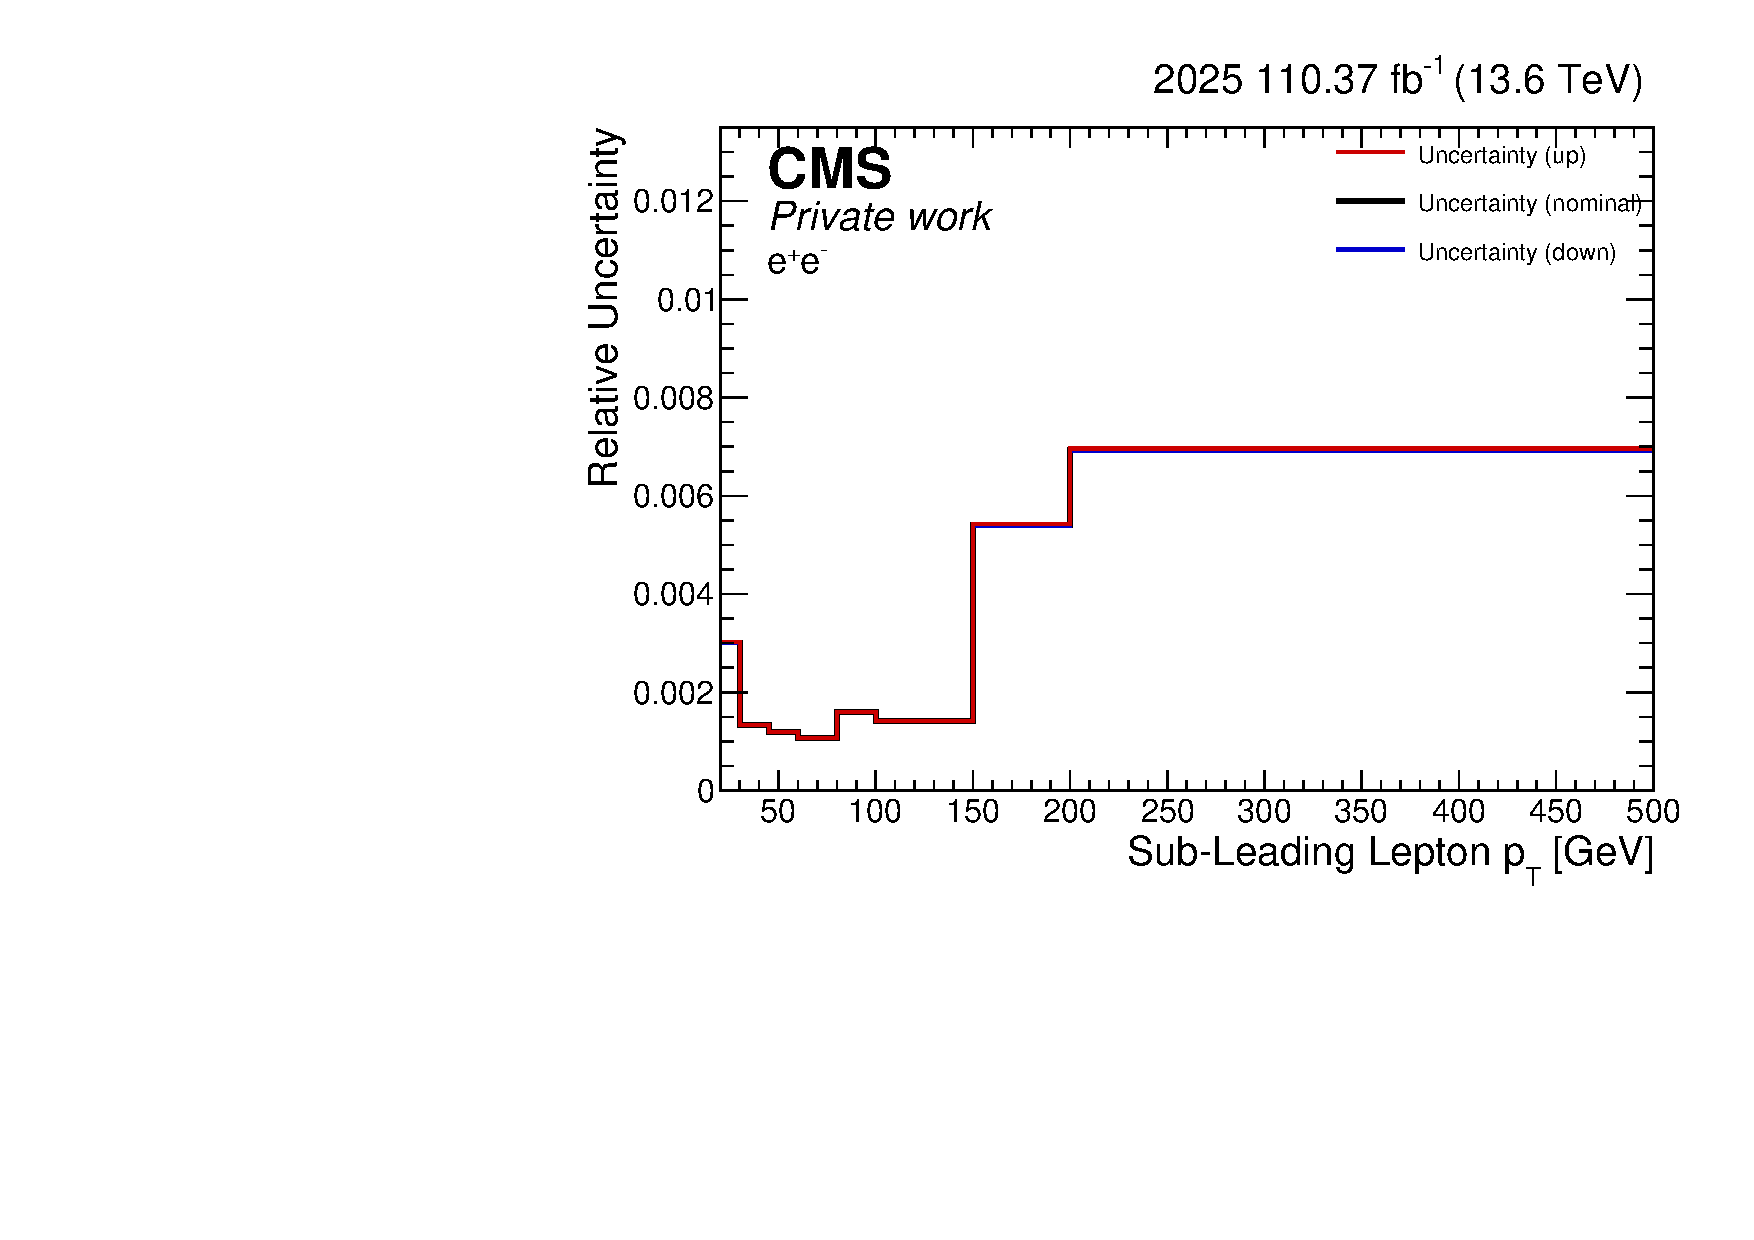
\includegraphics[width=0.48\linewidth]{figures/2025/ElEl/Statistical_Uncertainty/UncRatio_Lep2pt.pdf}
\caption{Relative statistical uncertainty diagnostics, retaining the nominal, upward, and downward curves of the supplied production in the $ee$ channel. Left and right: leading and subleading lepton $p_{\mathrm{T}}$.}\label{fig:extra-ElEl-Statistical-Uncertainty-Lep1pt-2025}\end{figure}
\begin{figure}[p]\centering
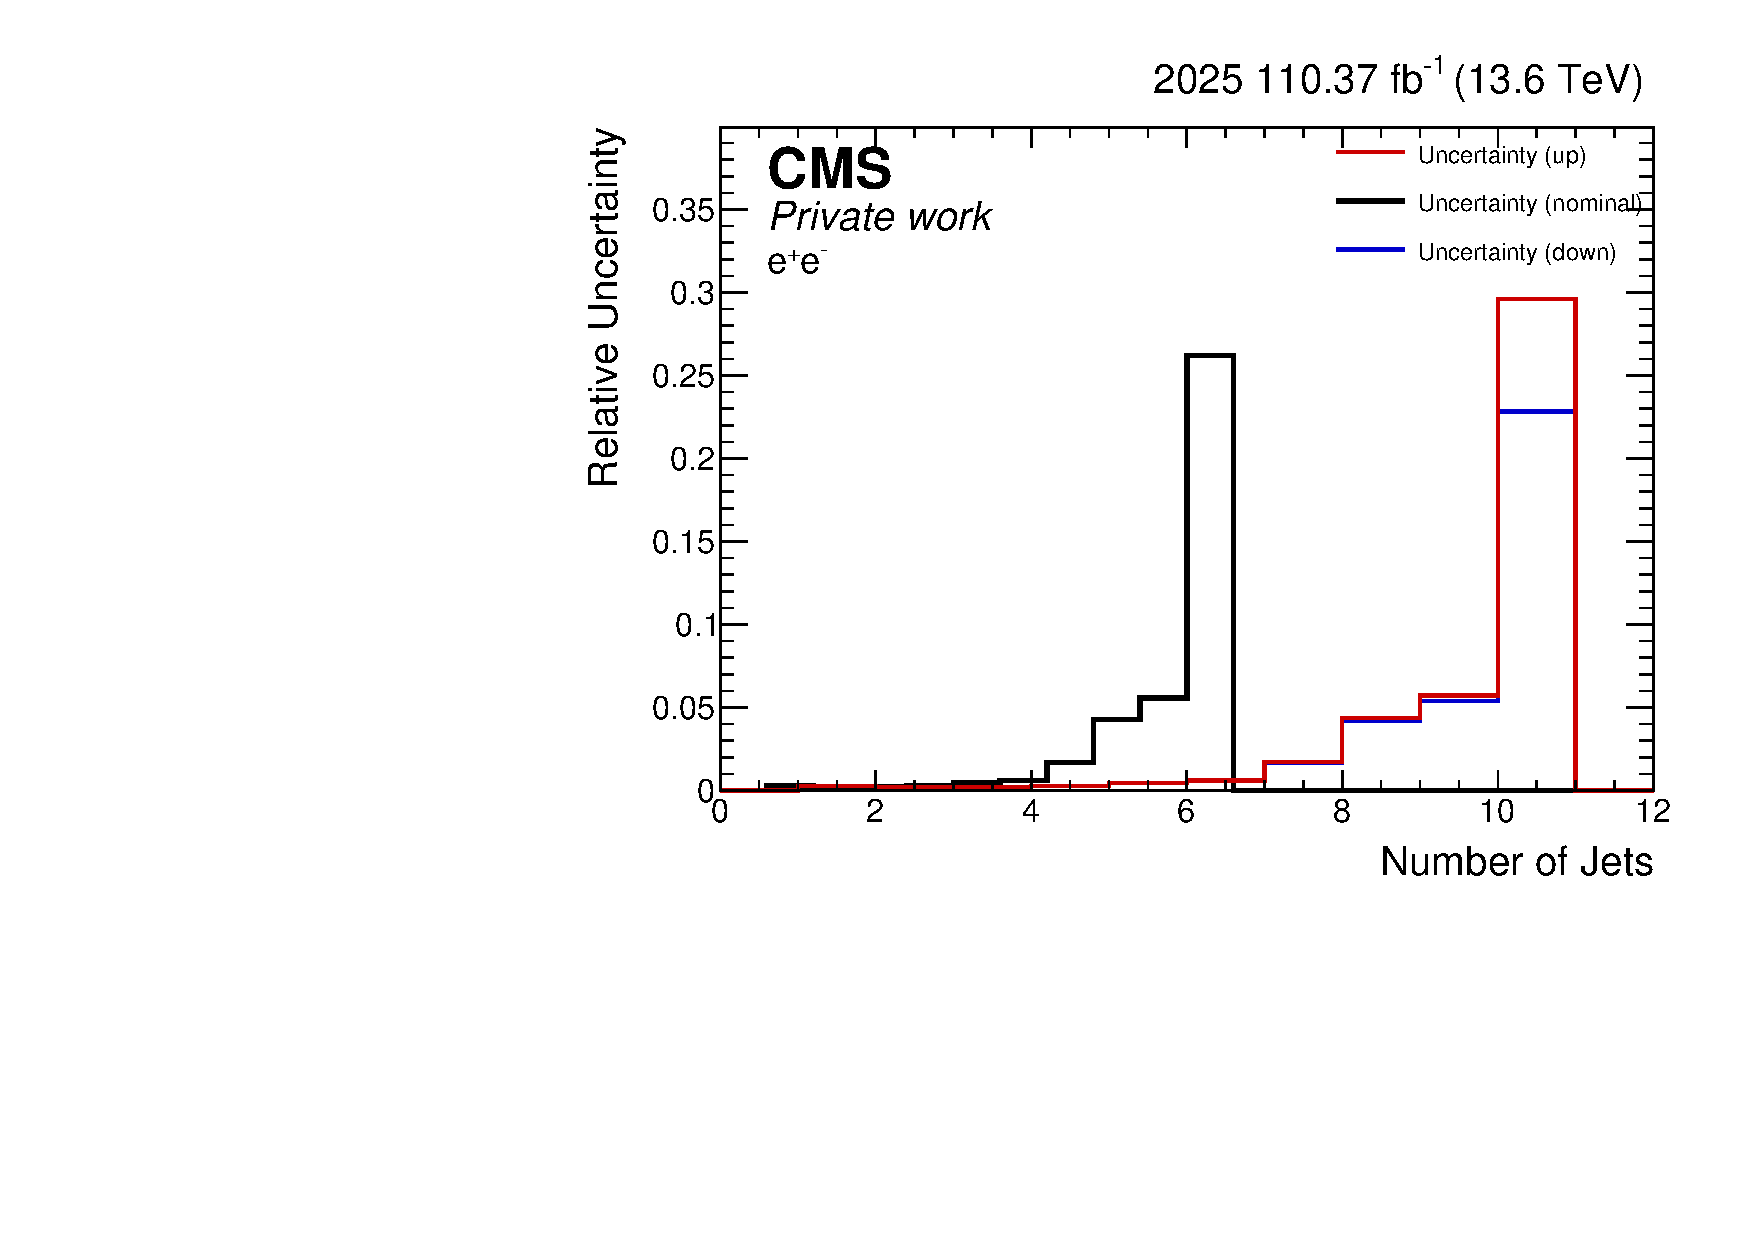
\includegraphics[width=0.48\linewidth]{figures/2025/ElEl/Statistical_Uncertainty/UncRatio_Num_Jets.pdf}
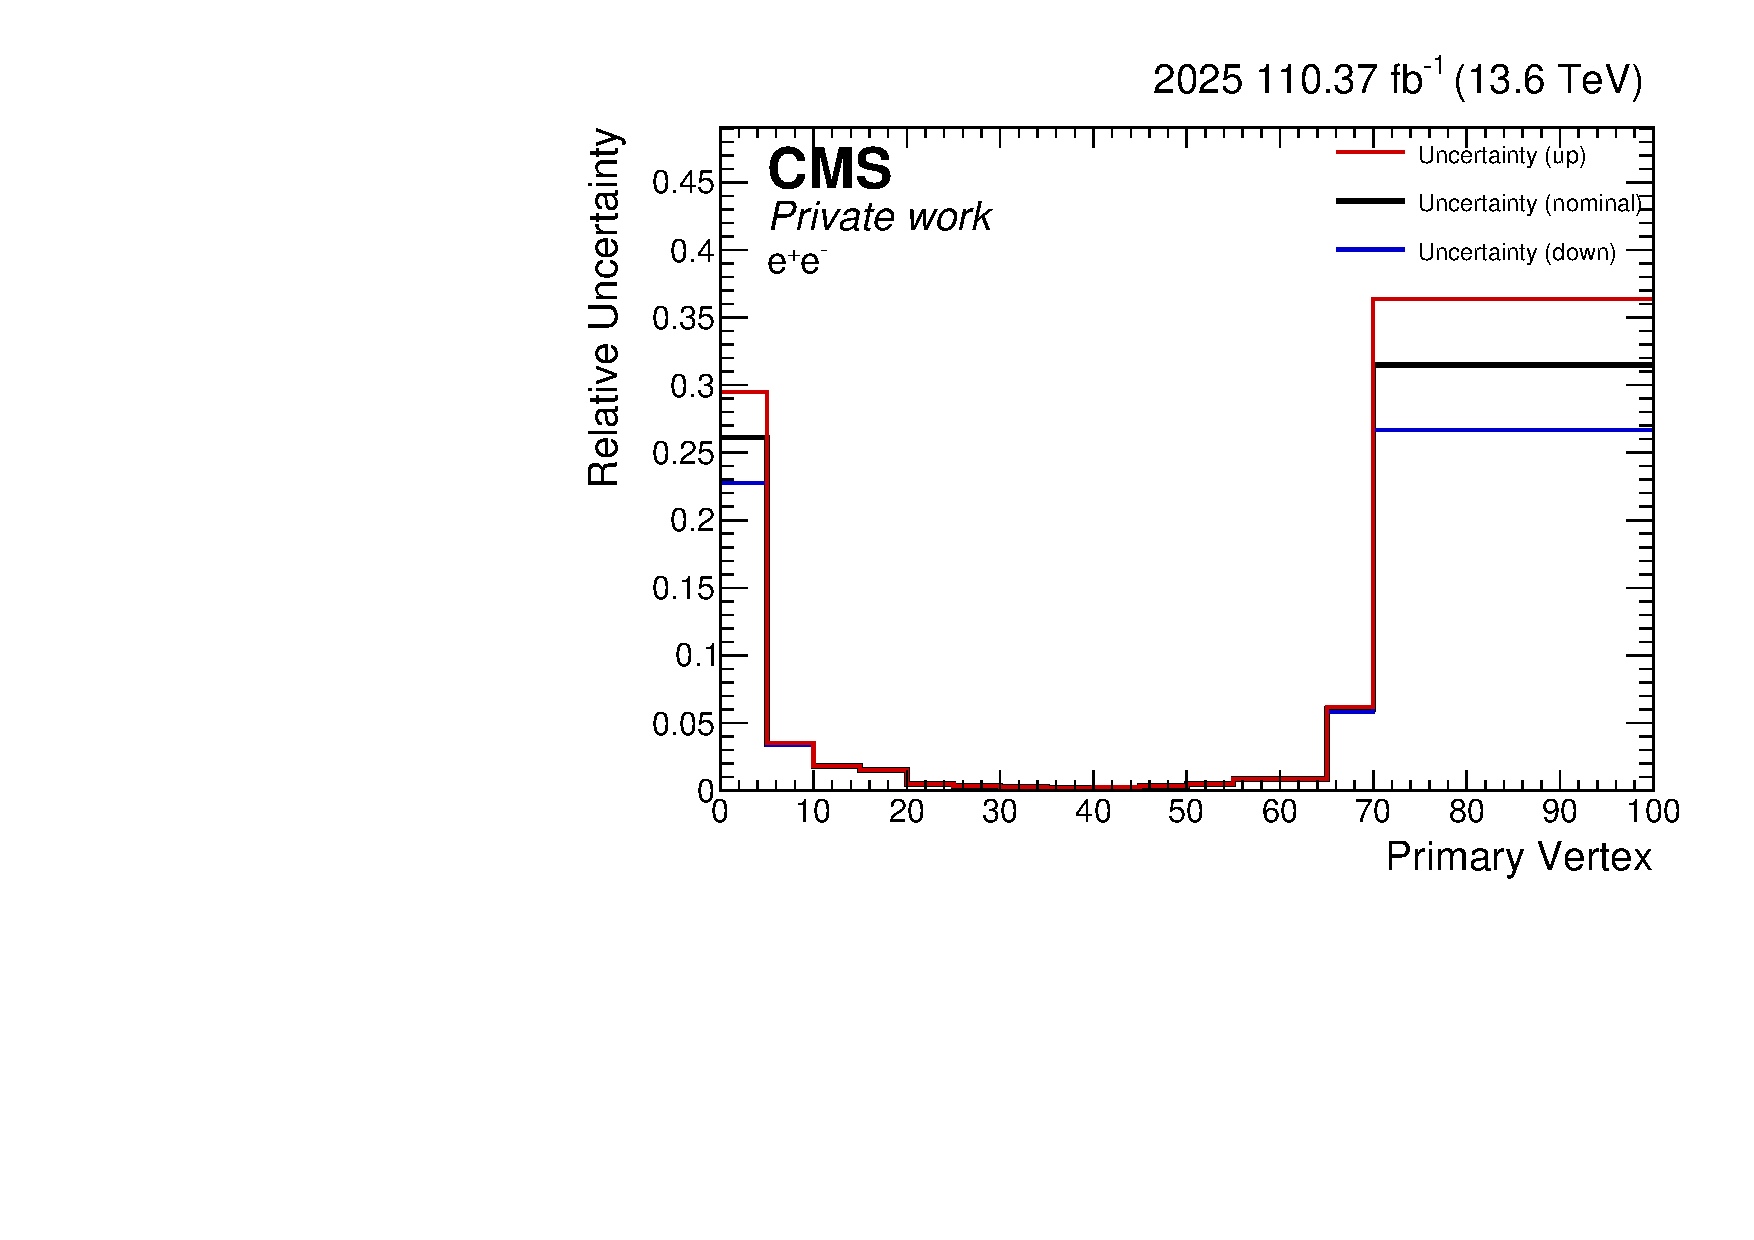
\includegraphics[width=0.48\linewidth]{figures/2025/ElEl/Statistical_Uncertainty/UncRatio_Num_PV.pdf}
\caption{Relative statistical uncertainty diagnostics, retaining the nominal, upward, and downward curves of the supplied production in the $ee$ channel. Left and right: jet and primary-vertex multiplicities.}\label{fig:extra-ElEl-Statistical-Uncertainty-Num_Jets-2025}\end{figure}
\begin{figure}[p]\centering
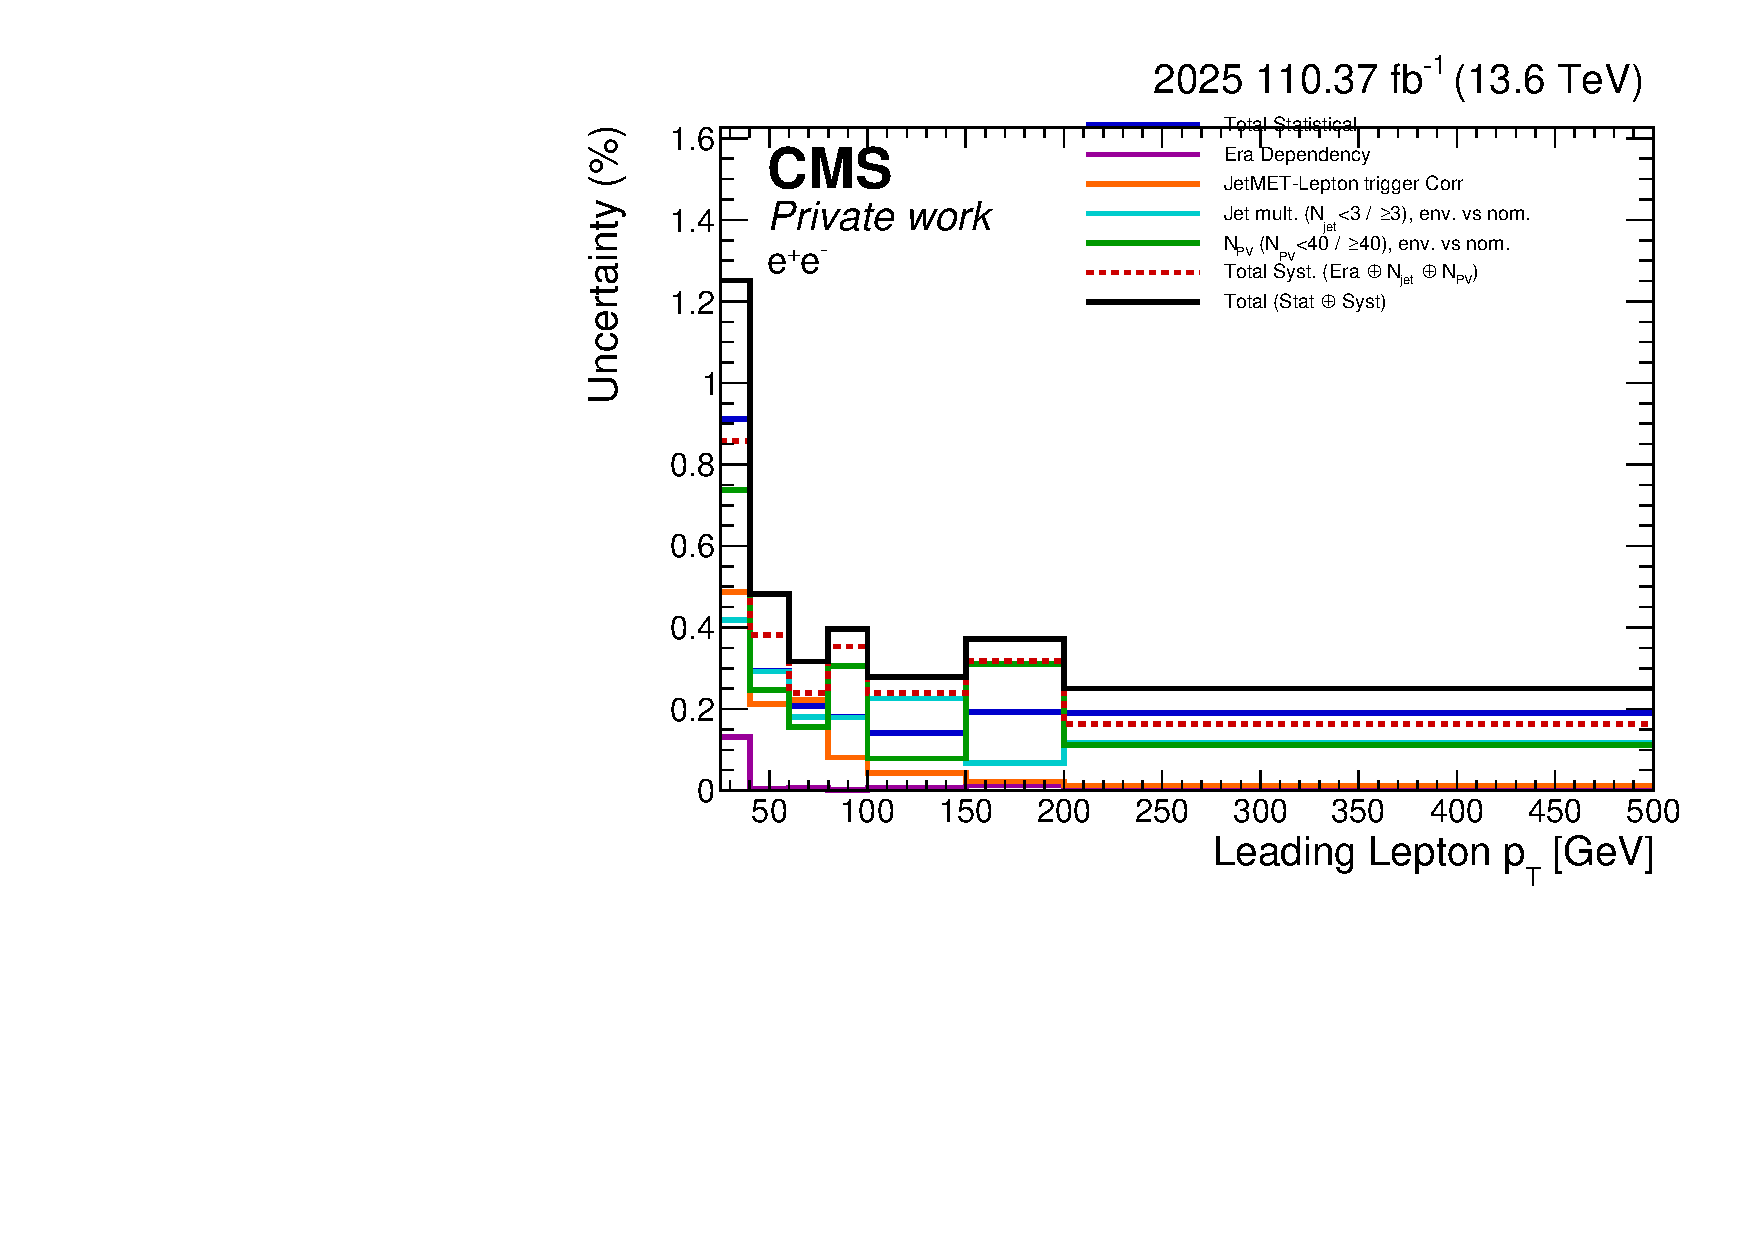
\includegraphics[width=0.48\linewidth]{figures/2025/ElEl/Uncertainty_Breakdown/Breakdown_Lep1pt.pdf}
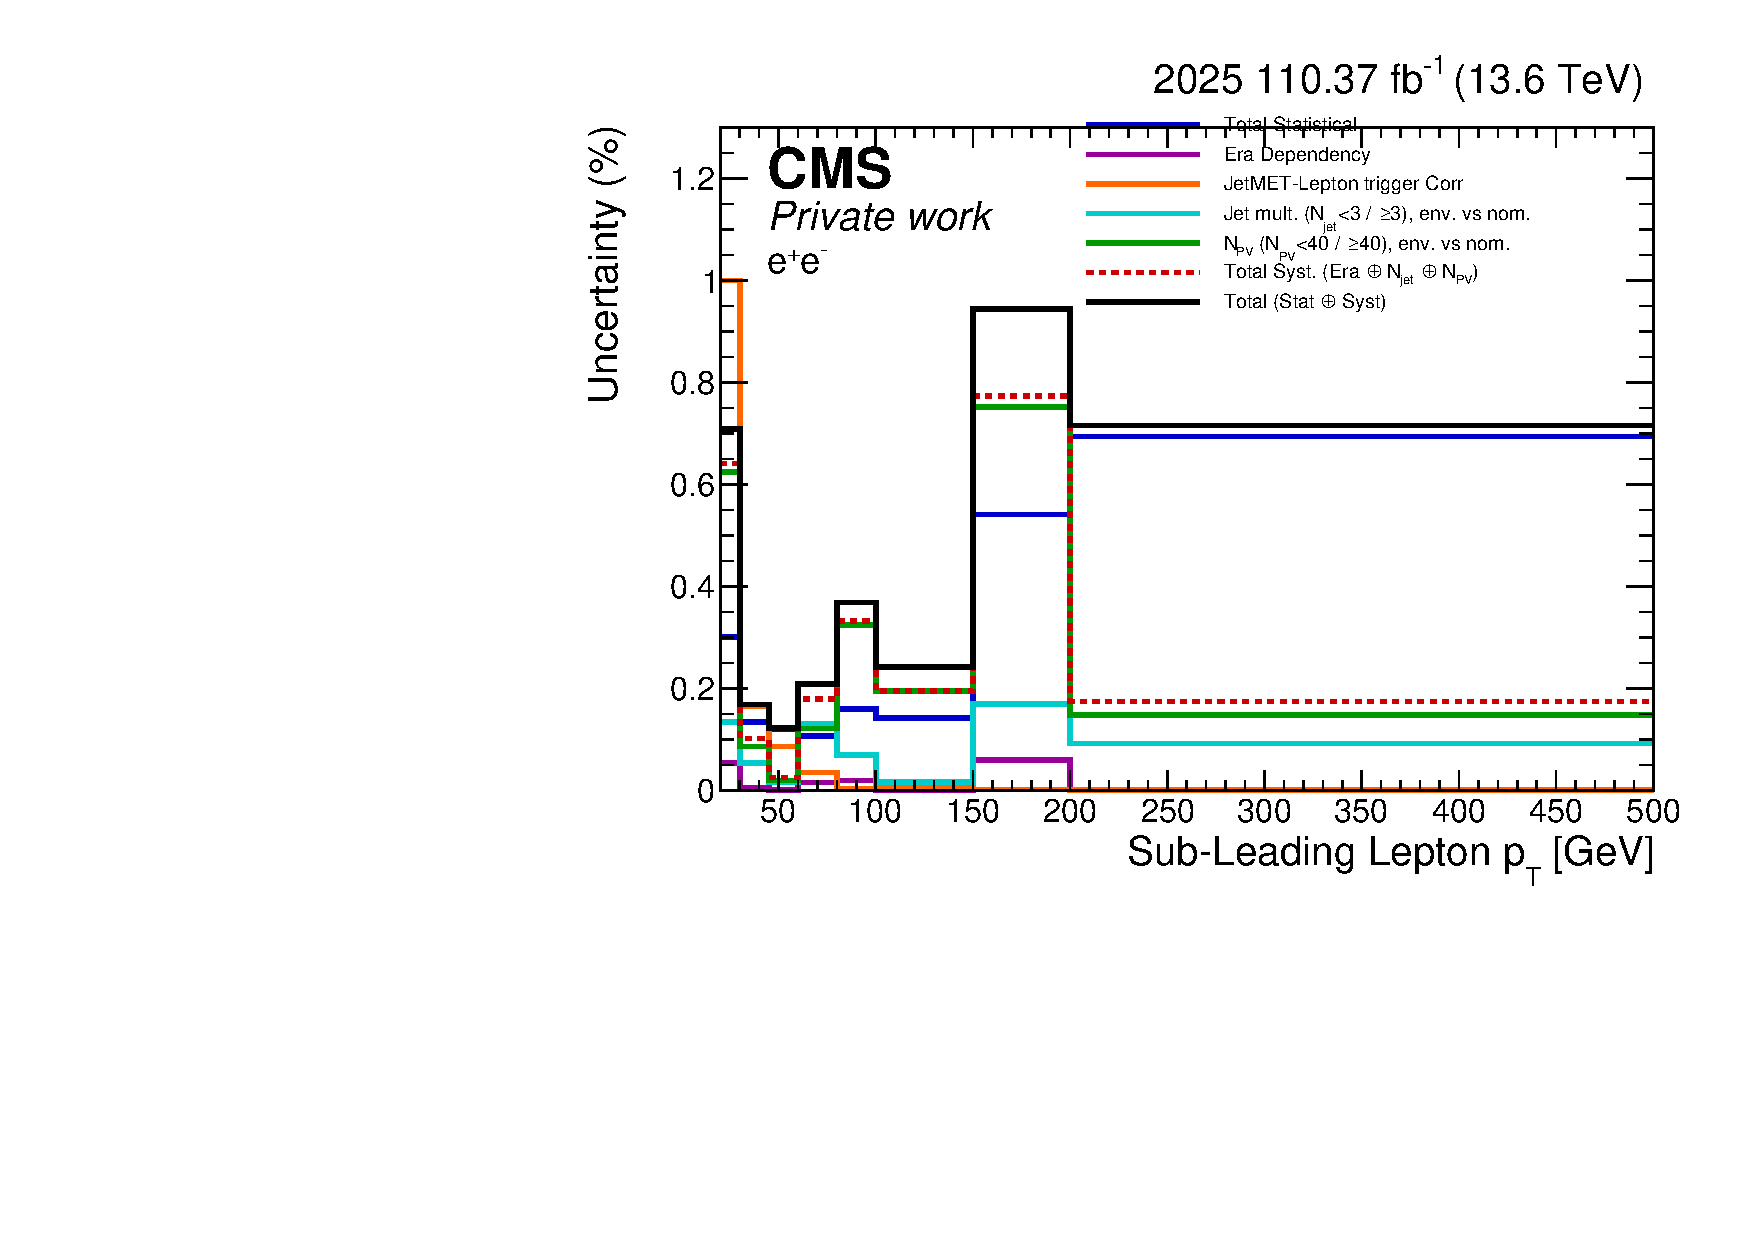
\includegraphics[width=0.48\linewidth]{figures/2025/ElEl/Uncertainty_Breakdown/Breakdown_Lep2pt.pdf}
\caption{Absolute uncertainty component breakdown in the $ee$ channel. Left and right: leading and subleading lepton $p_{\mathrm{T}}$.}\label{fig:extra-ElEl-Uncertainty-Breakdown-Lep1pt-2025}\end{figure}
\begin{figure}[p]\centering
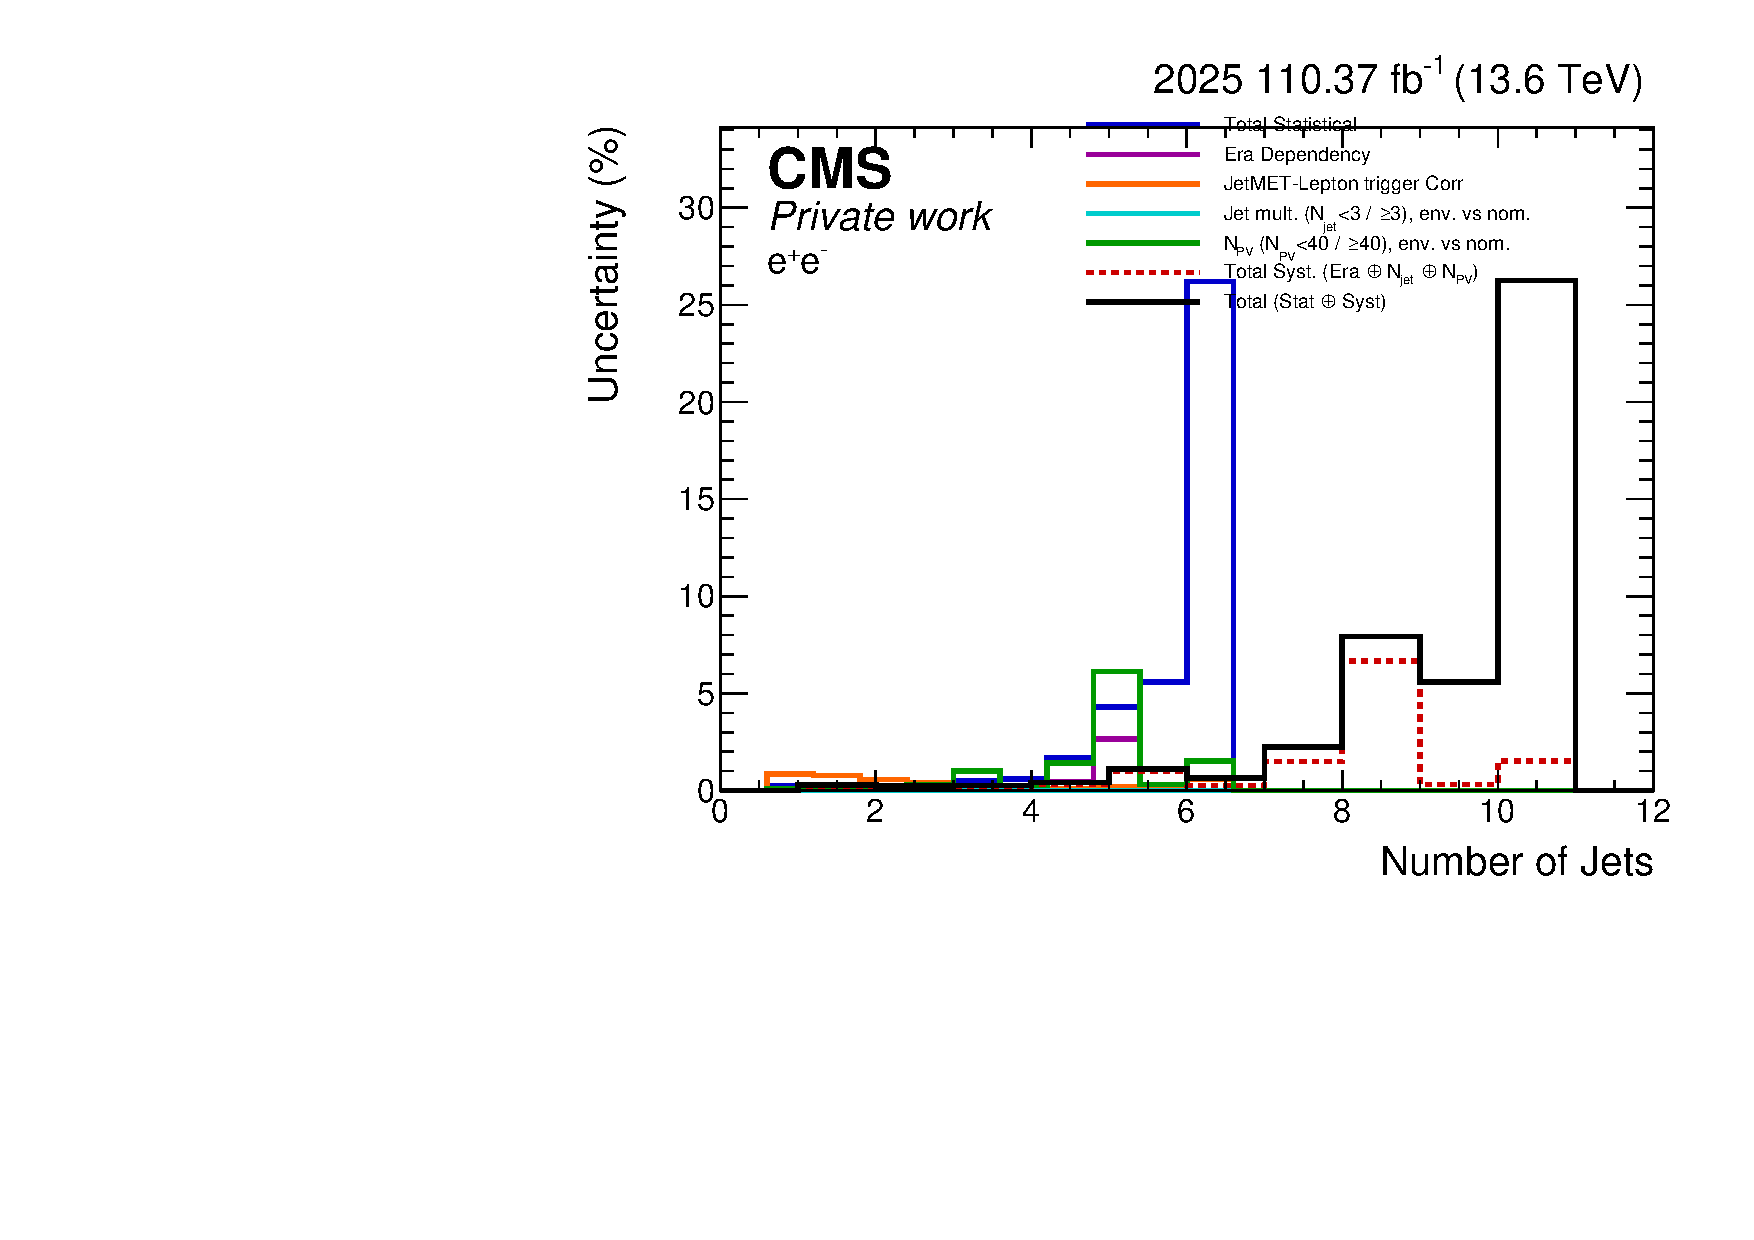
\includegraphics[width=0.48\linewidth]{figures/2025/ElEl/Uncertainty_Breakdown/Breakdown_Num_Jets.pdf}
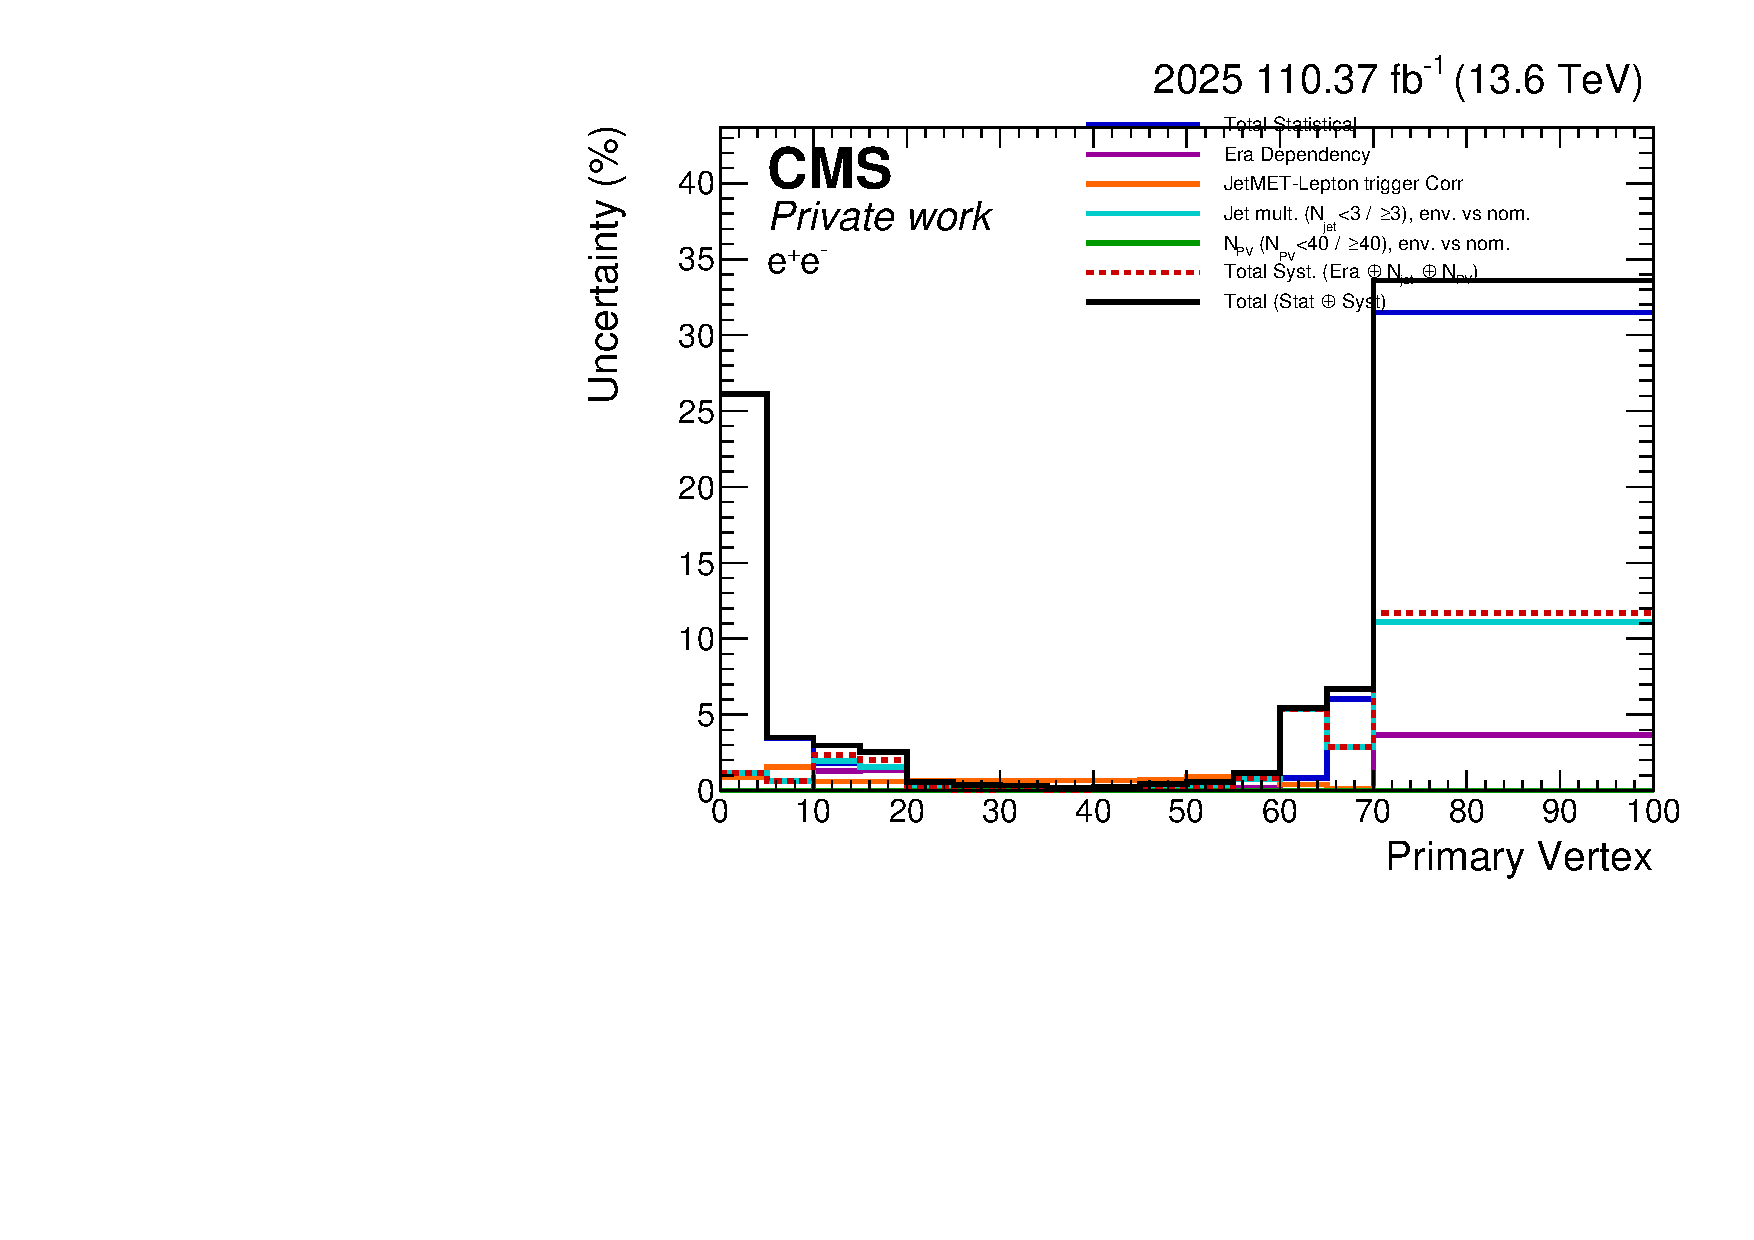
\includegraphics[width=0.48\linewidth]{figures/2025/ElEl/Uncertainty_Breakdown/Breakdown_Num_PV.pdf}
\caption{Absolute uncertainty component breakdown in the $ee$ channel. Left and right: jet and primary-vertex multiplicities.}\label{fig:extra-ElEl-Uncertainty-Breakdown-Num_Jets-2025}\end{figure}
\begin{figure}[p]\centering
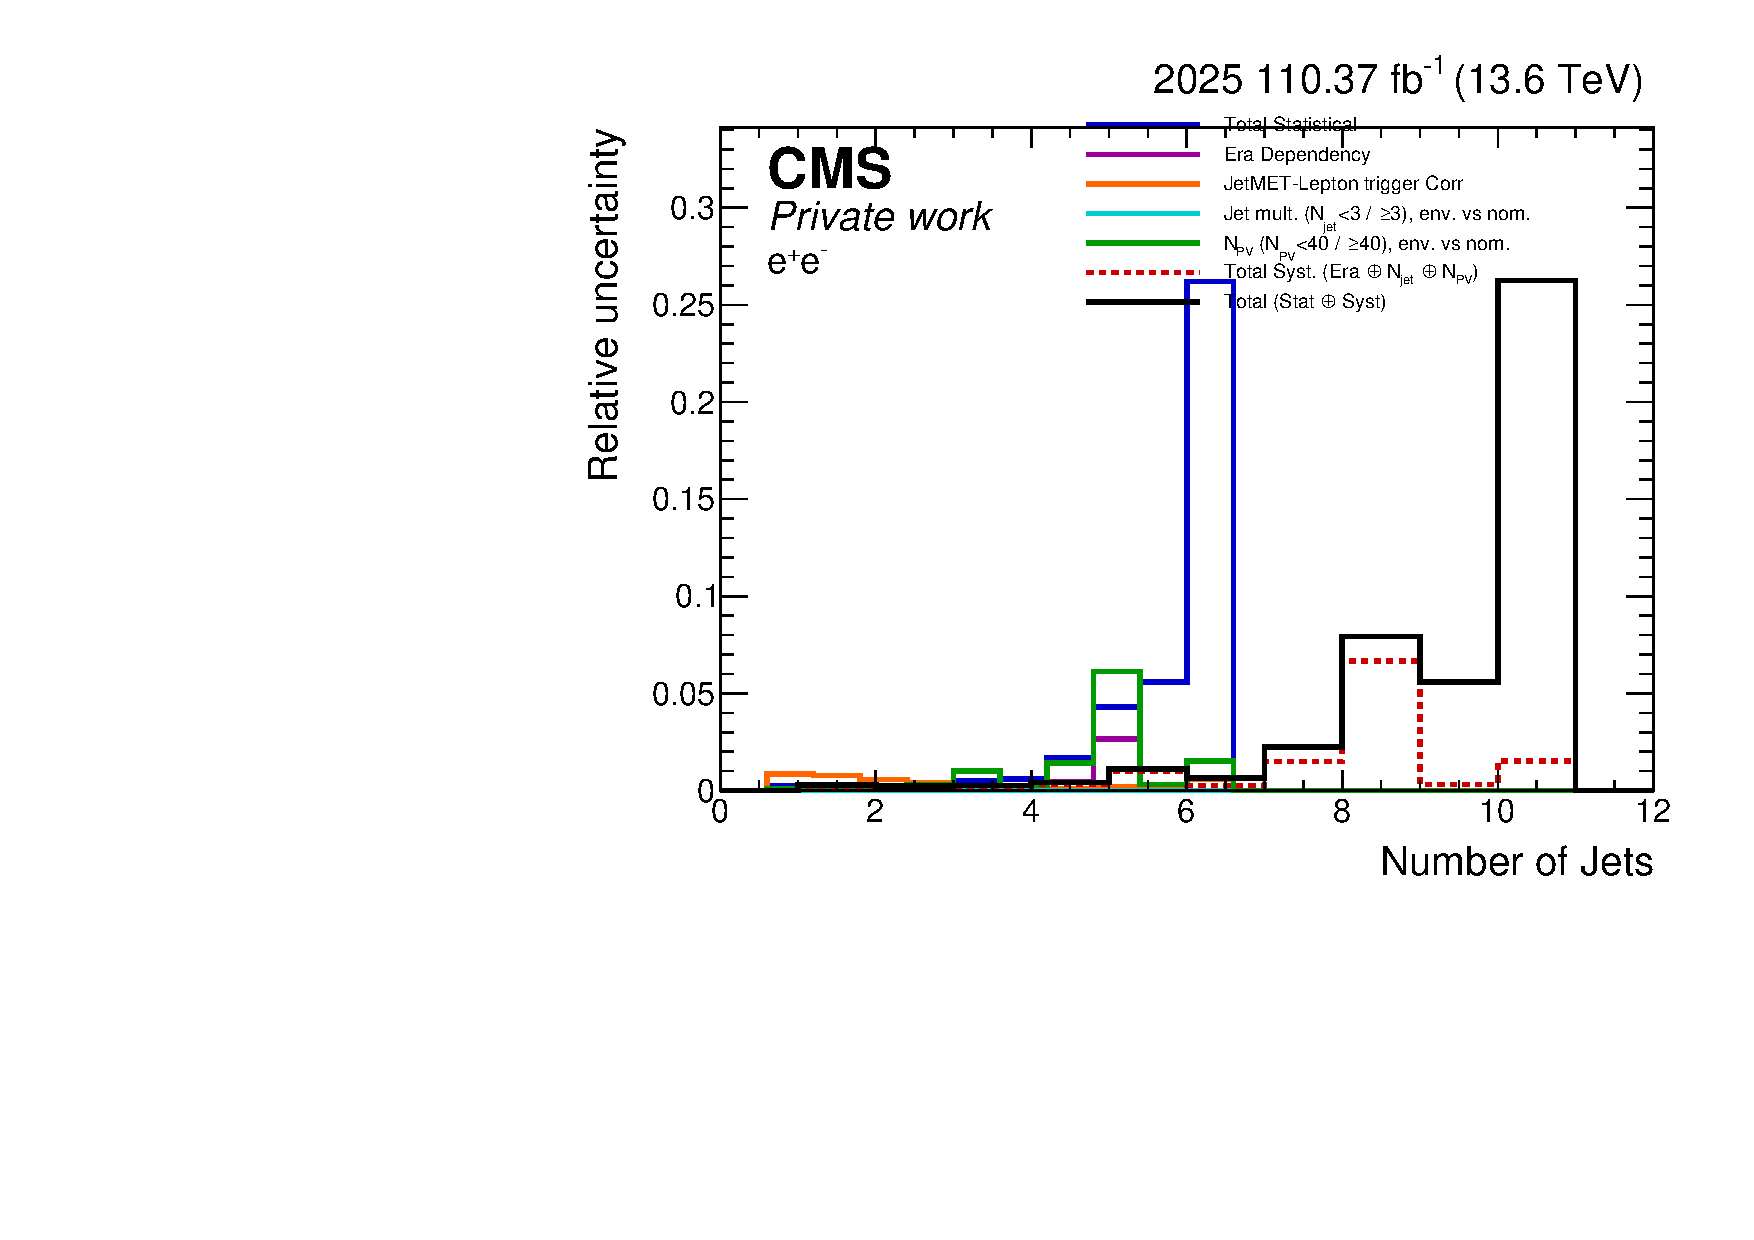
\includegraphics[width=0.48\linewidth]{figures/2025/ElEl/Relative_Uncertainty_Breakdown/Breakdown_Num_Jets.pdf}
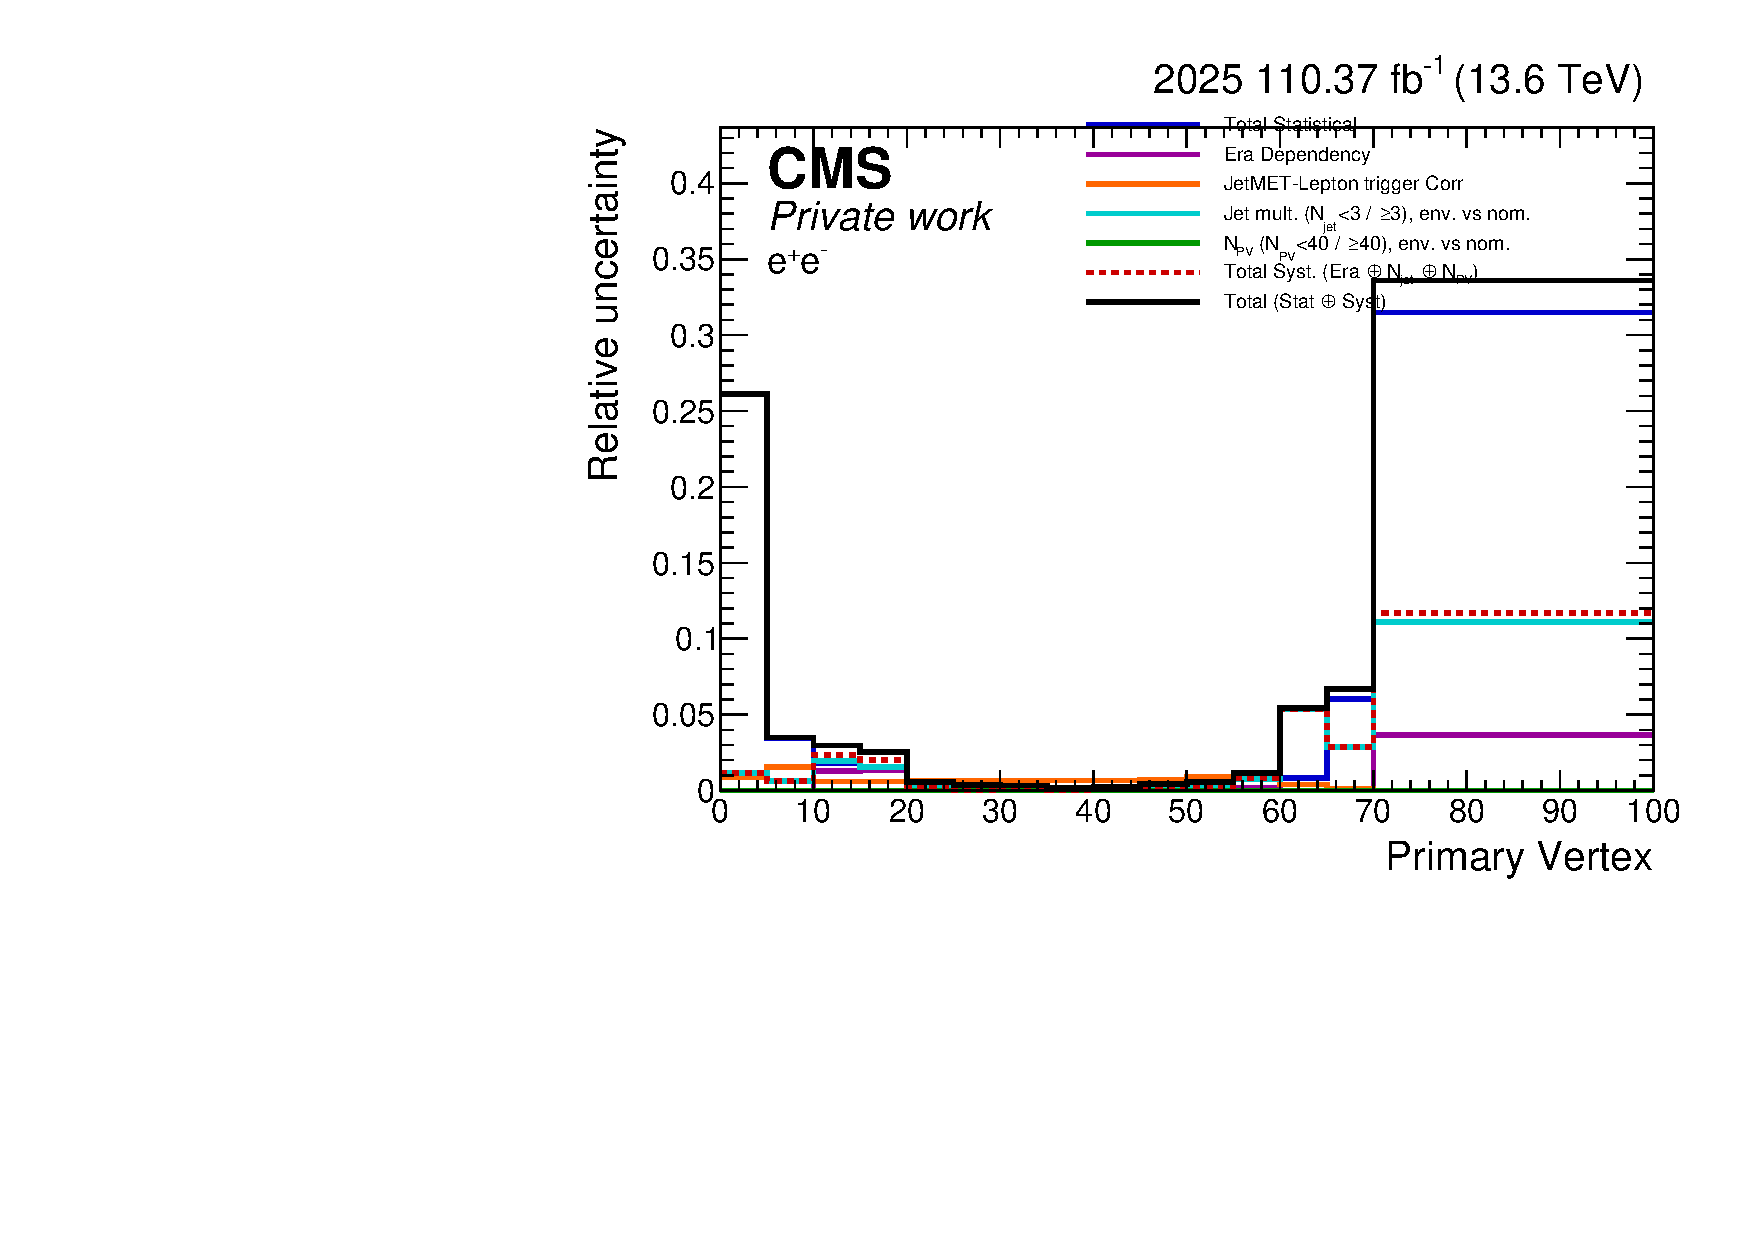
\includegraphics[width=0.48\linewidth]{figures/2025/ElEl/Relative_Uncertainty_Breakdown/Breakdown_Num_PV.pdf}
\caption{Relative uncertainty component breakdown versus event activity in the $ee$ channel. Left and right: jet and primary-vertex multiplicities.}\label{fig:extra-ElEl-Relative-Uncertainty-Breakdown-Num_Jets-2025}\end{figure}
\begin{figure}[p]\centering
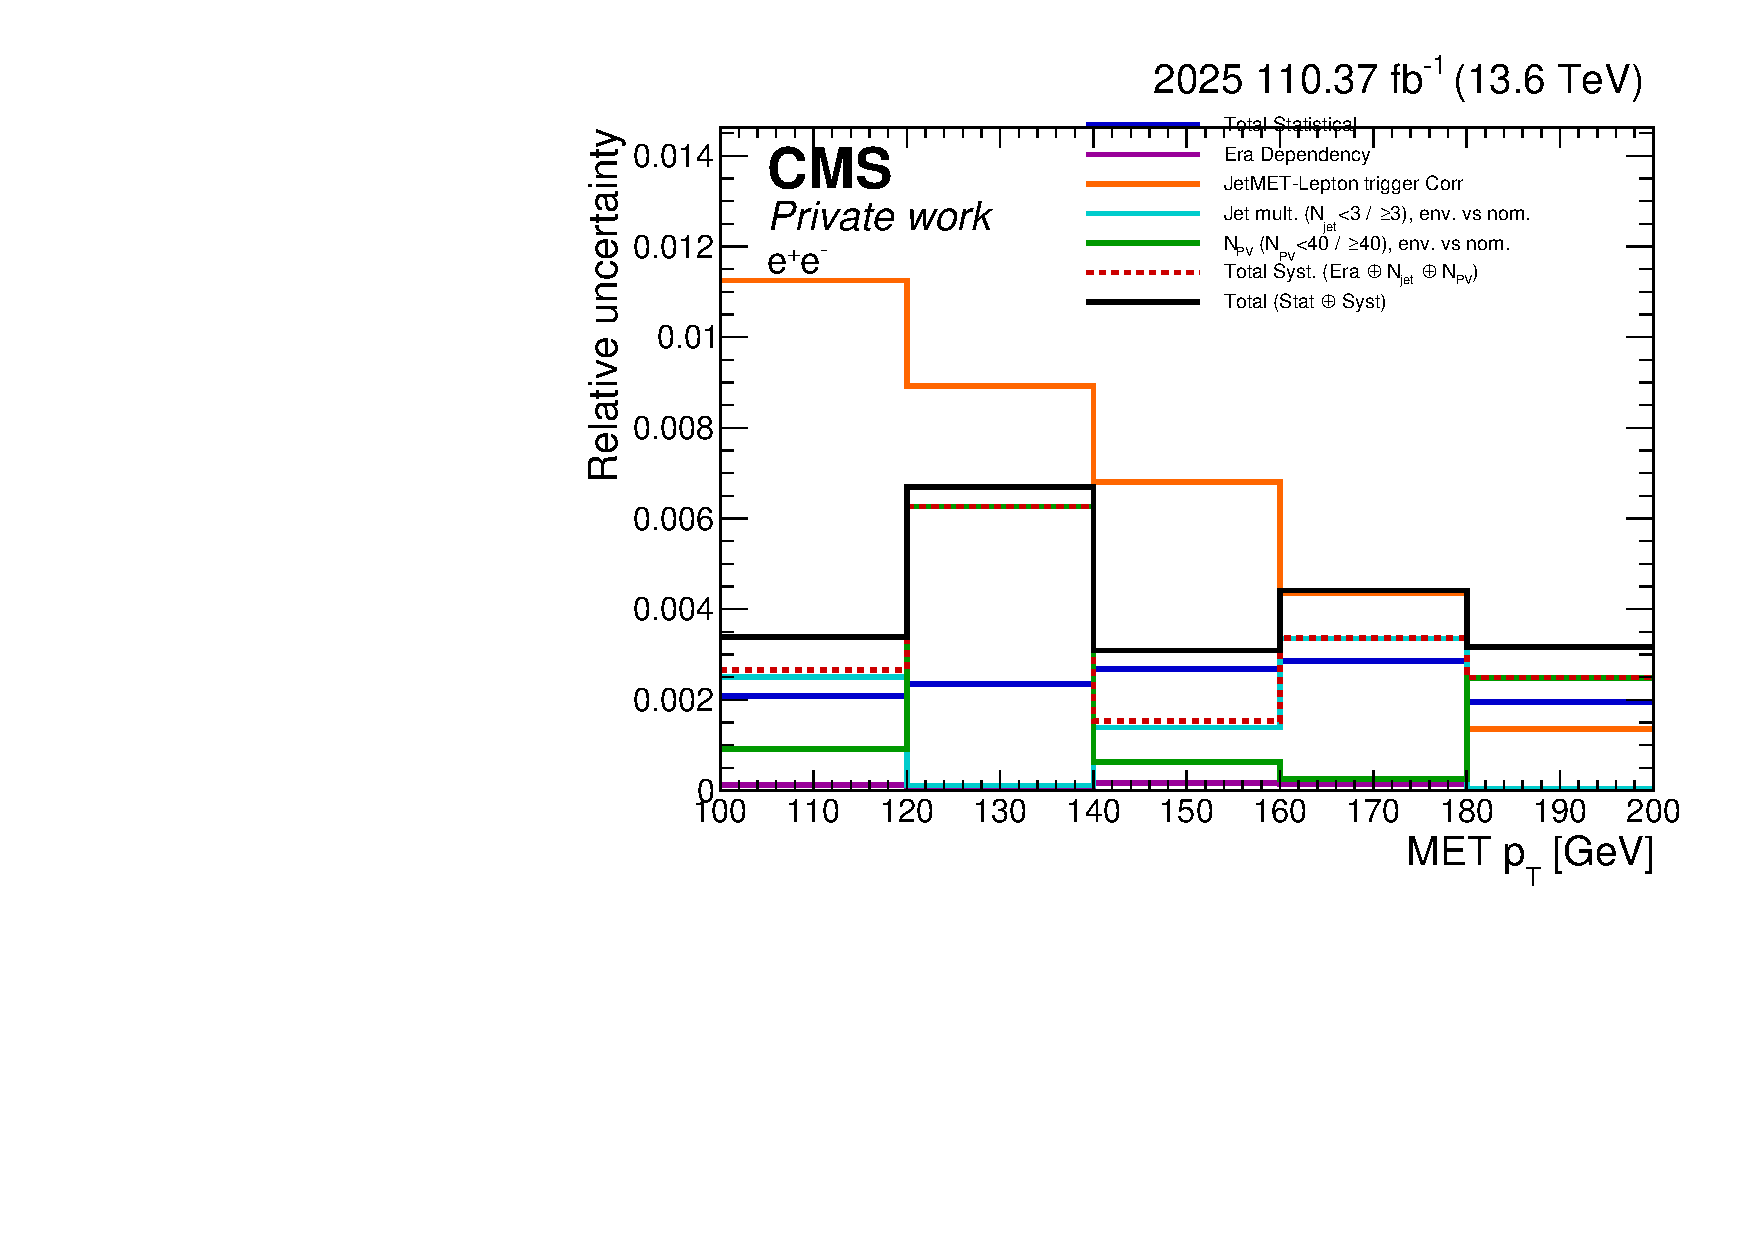
\includegraphics[width=0.48\linewidth]{figures/2025/ElEl/Relative_Uncertainty_Breakdown/Breakdown_METpt.pdf}
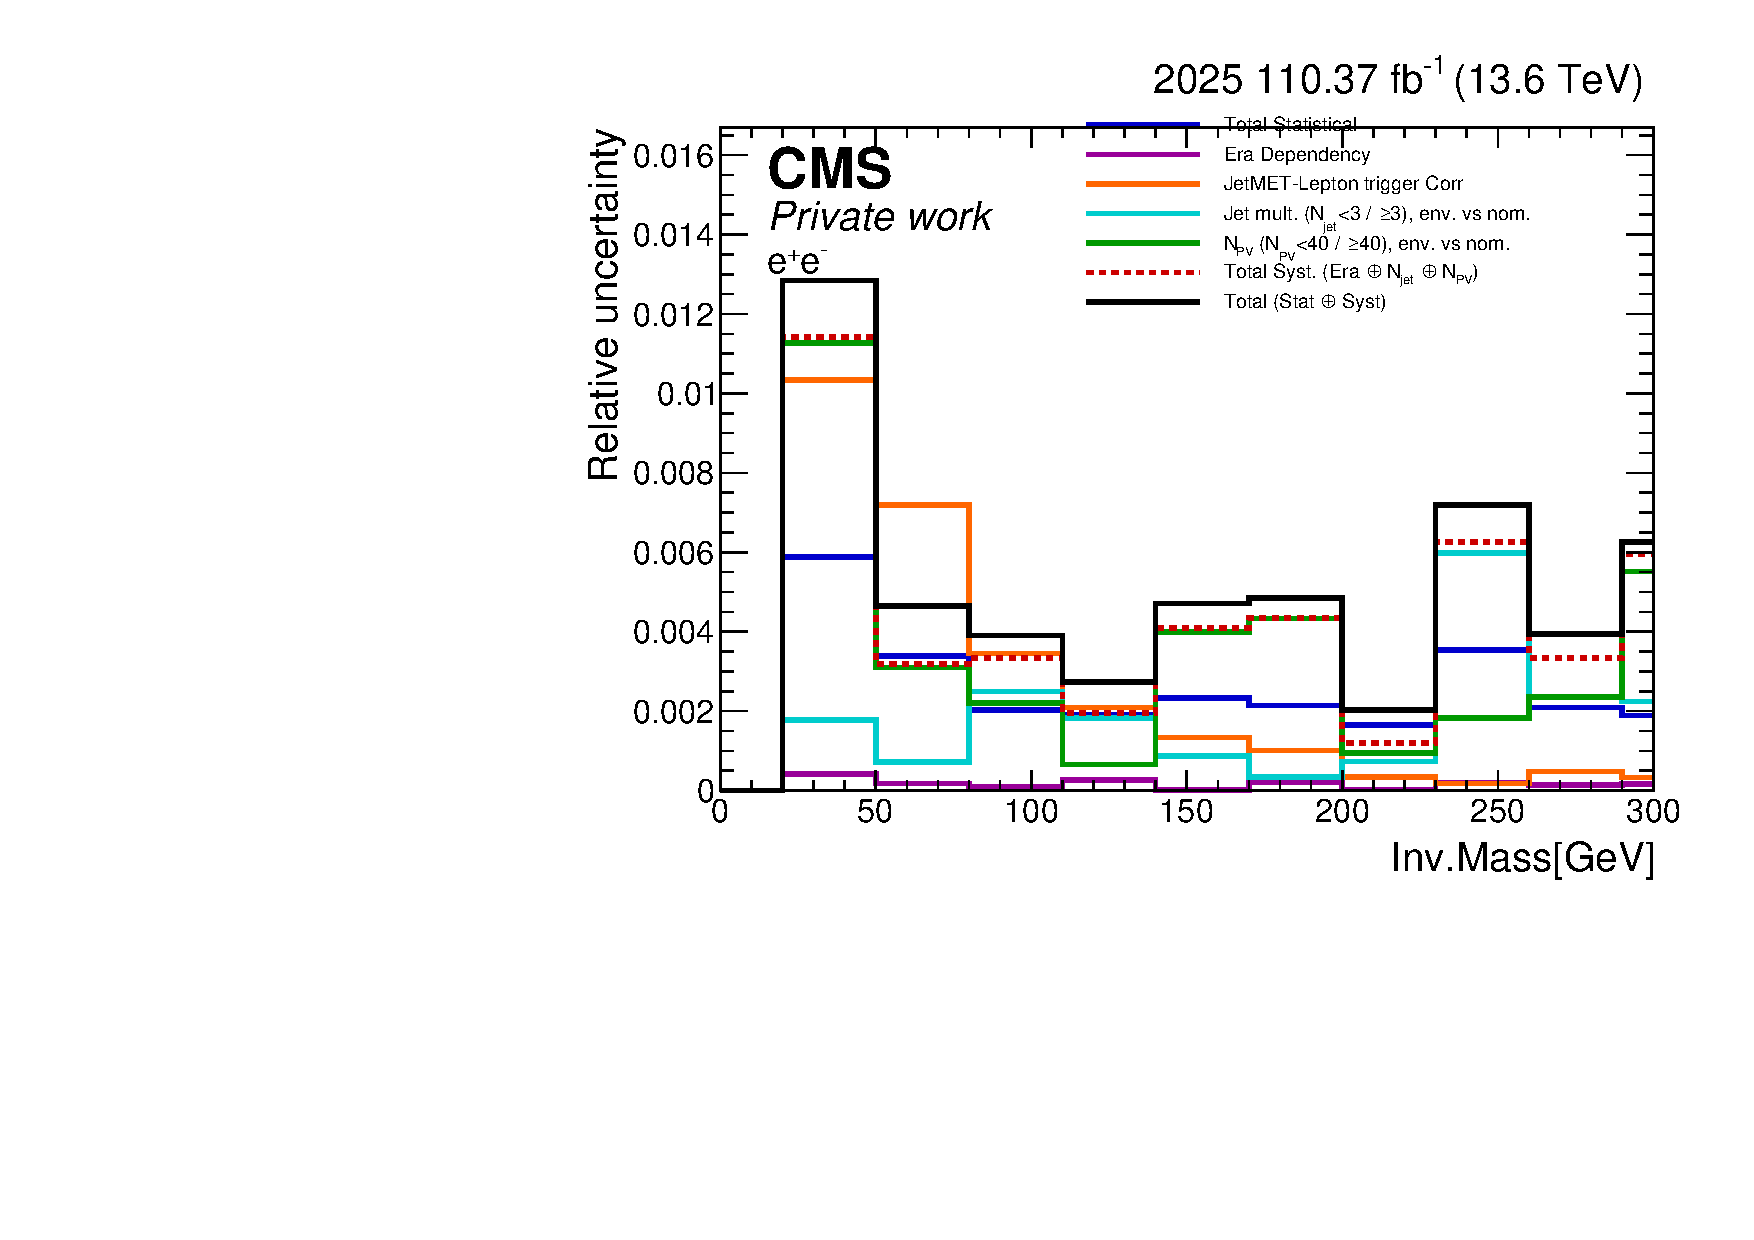
\includegraphics[width=0.48\linewidth]{figures/2025/ElEl/Relative_Uncertainty_Breakdown/Breakdown_DiLepMass.pdf}
\caption{Relative uncertainty component breakdown versus event kinematics in the $ee$ channel. Left and right: missing transverse momentum and dilepton invariant mass.}\label{fig:extra-ElEl-Relative-Uncertainty-Breakdown-METpt-2025}\end{figure}
\begin{figure}[p]\centering
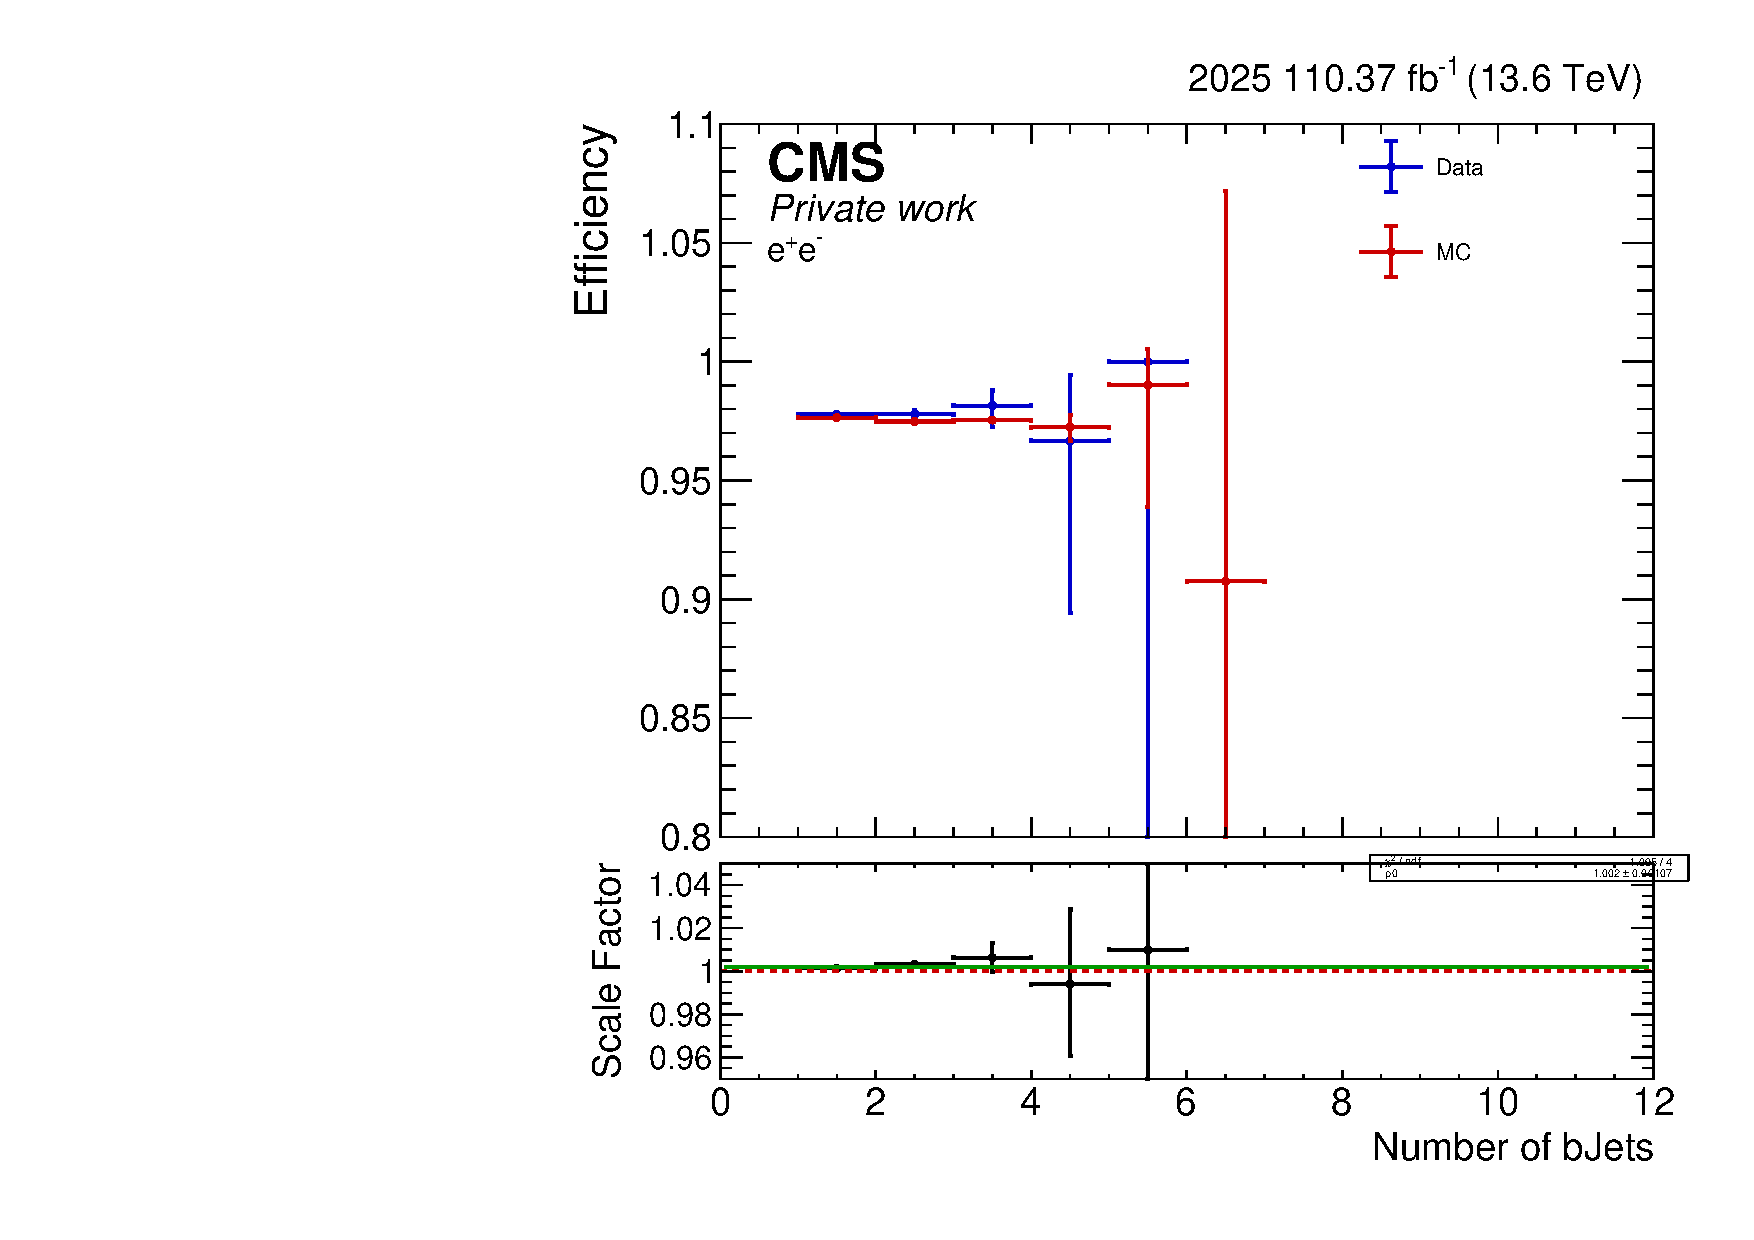
\includegraphics[width=0.48\linewidth]{figures/2025/ElEl/ScaleFactor/SF_Num_bJets.pdf}
\caption{Efficiency comparison and scale factor versus heavy-flavour activity in the $ee$ channel. $b$-tagged jet multiplicity.}\label{fig:extra-ElEl-ScaleFactor-Num_bJets-2025}\end{figure}
\clearpage\subsection{$e\mu$ channel}
\begin{figure}[p]\centering
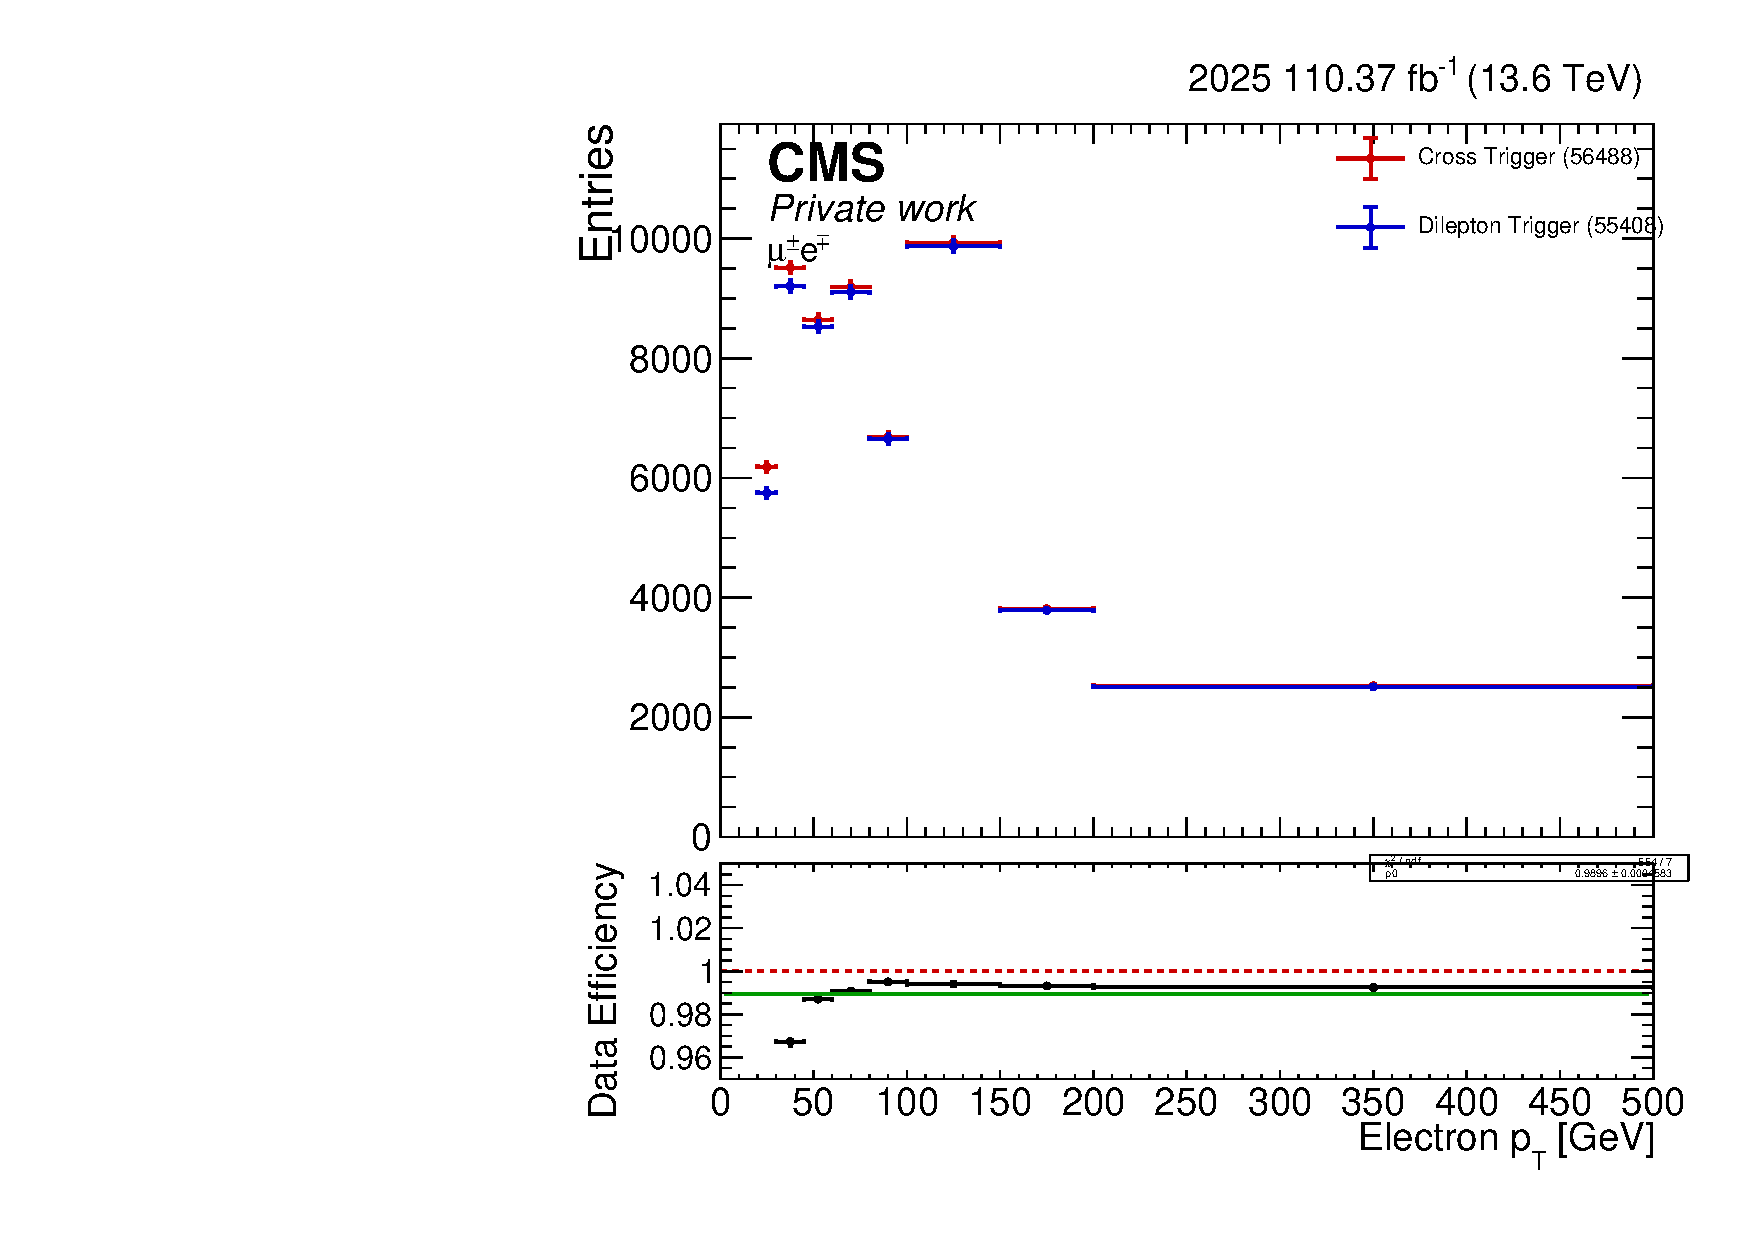
\includegraphics[width=0.48\linewidth]{figures/2025/MuEl/TrigEffData/TrigEff_ElPt.pdf}
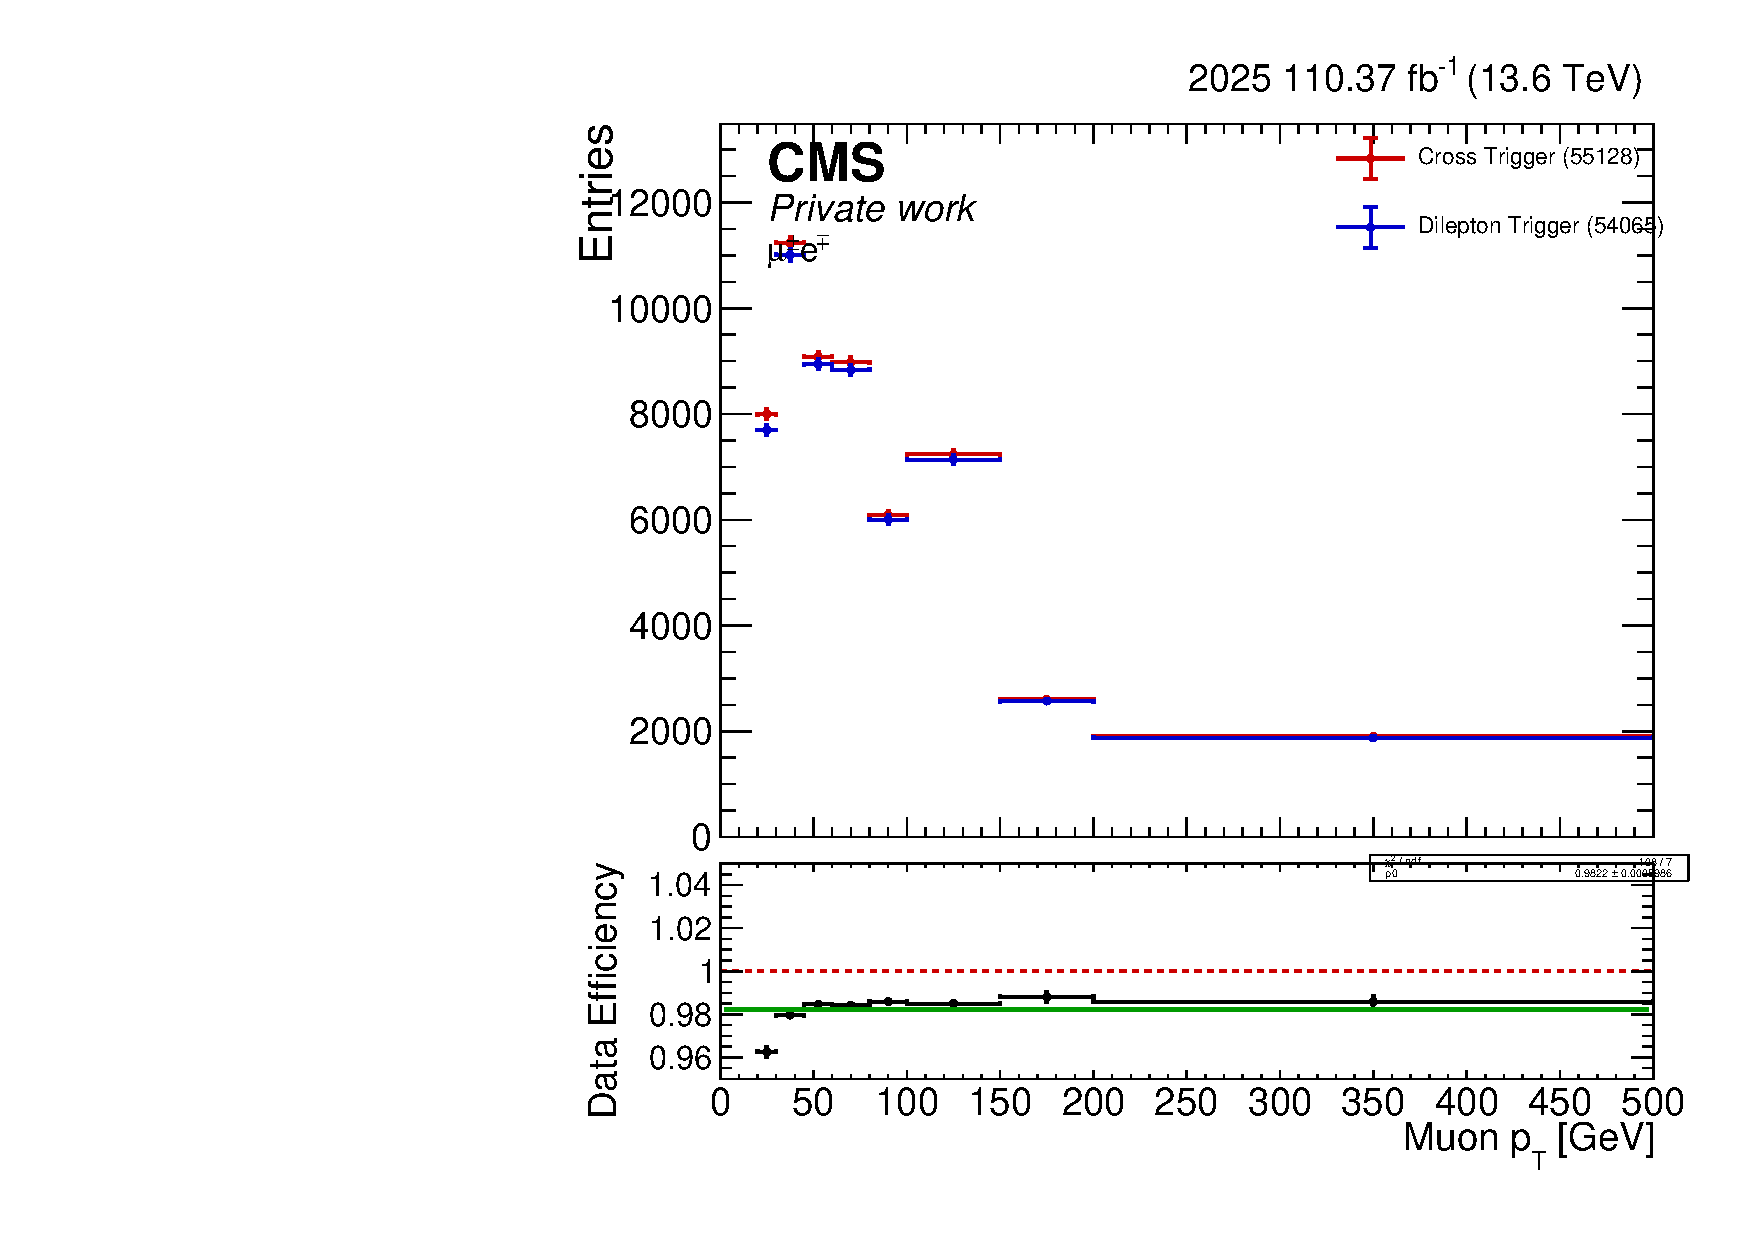
\includegraphics[width=0.48\linewidth]{figures/2025/MuEl/TrigEffData/TrigEff_MuPt.pdf}
\caption{Data trigger numerator and reference-sample distributions (upper panels), with their efficiency ratios (lower panels) in the $e\mu$ channel. Left and right: electron and muon $p_{\mathrm{T}}$.}\label{fig:extra-MuEl-TrigEffData-ElPt-2025}\end{figure}
\begin{figure}[p]\centering
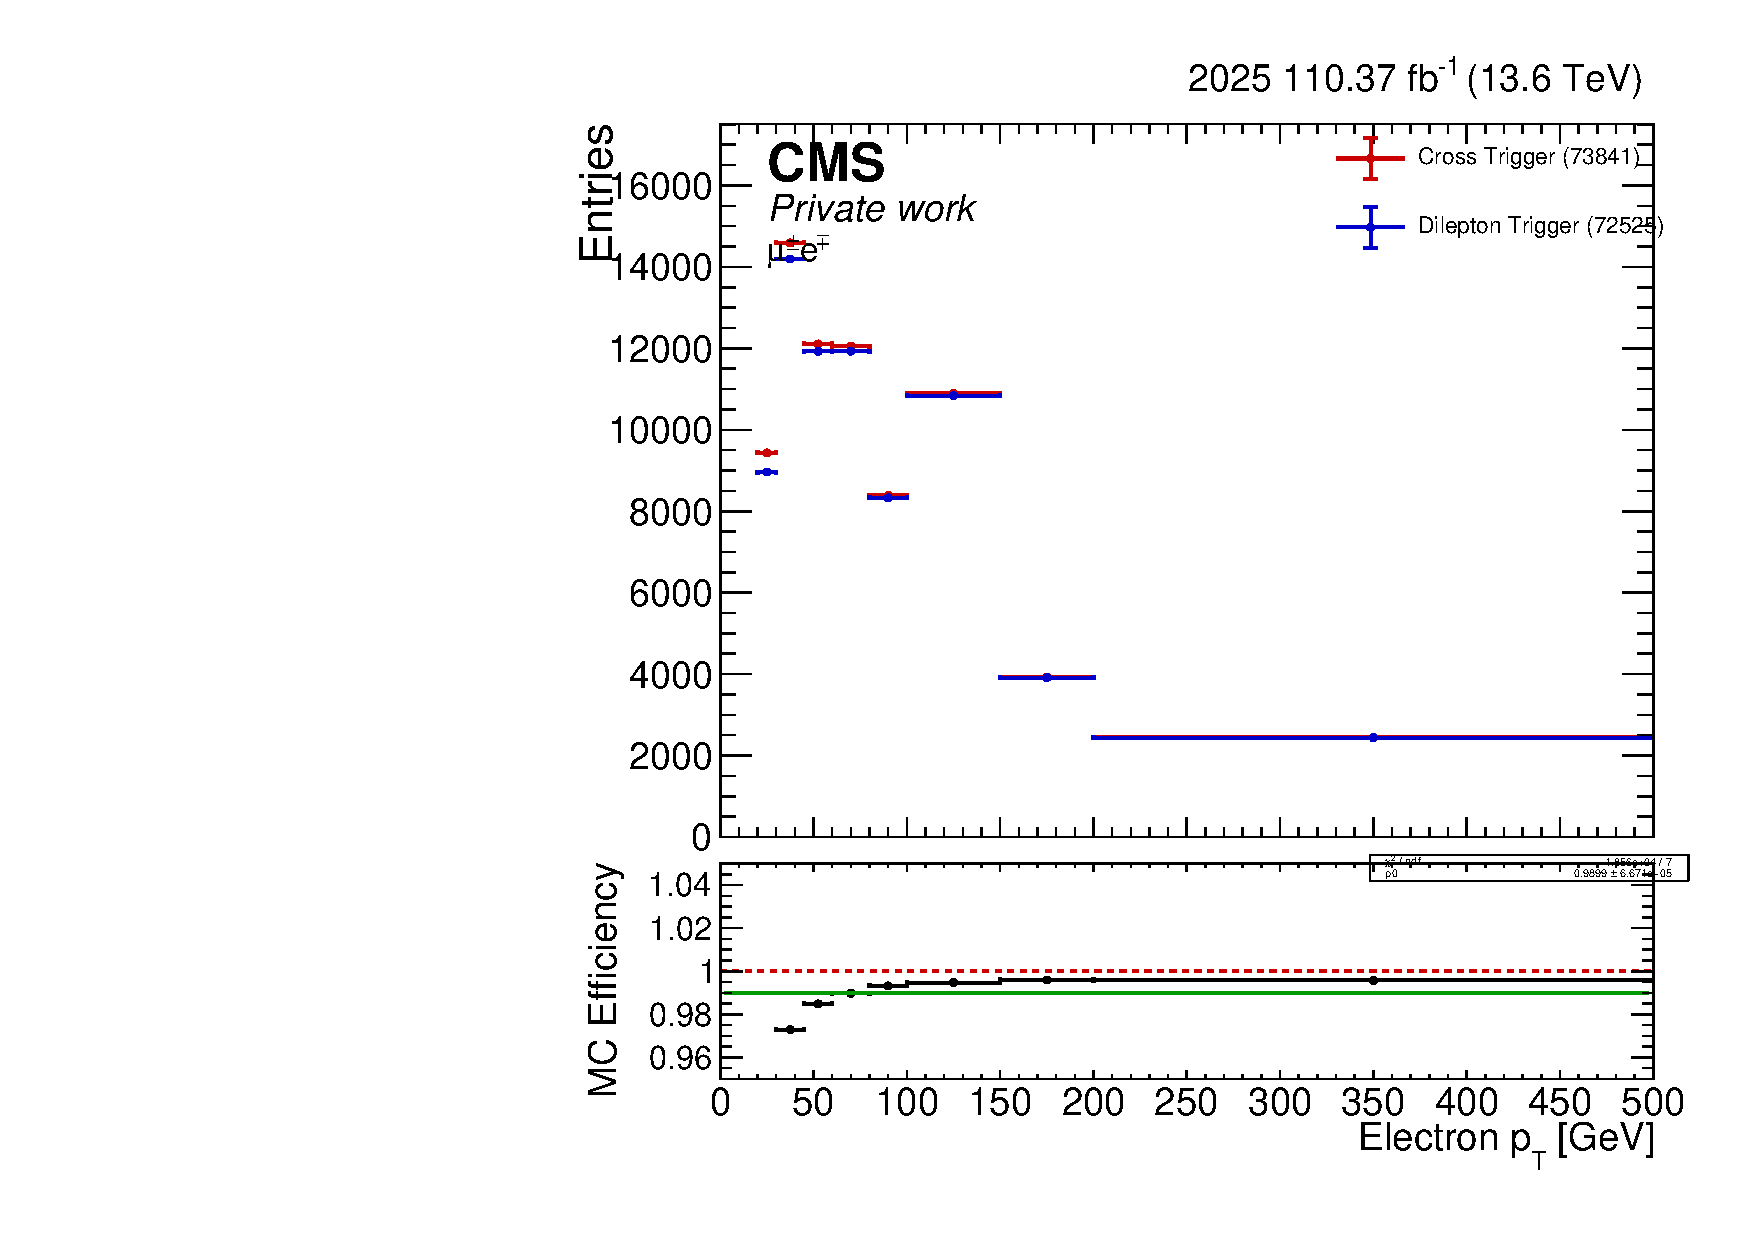
\includegraphics[width=0.48\linewidth]{figures/2025/MuEl/TrigEffMC/TrigEff_ElPt.pdf}
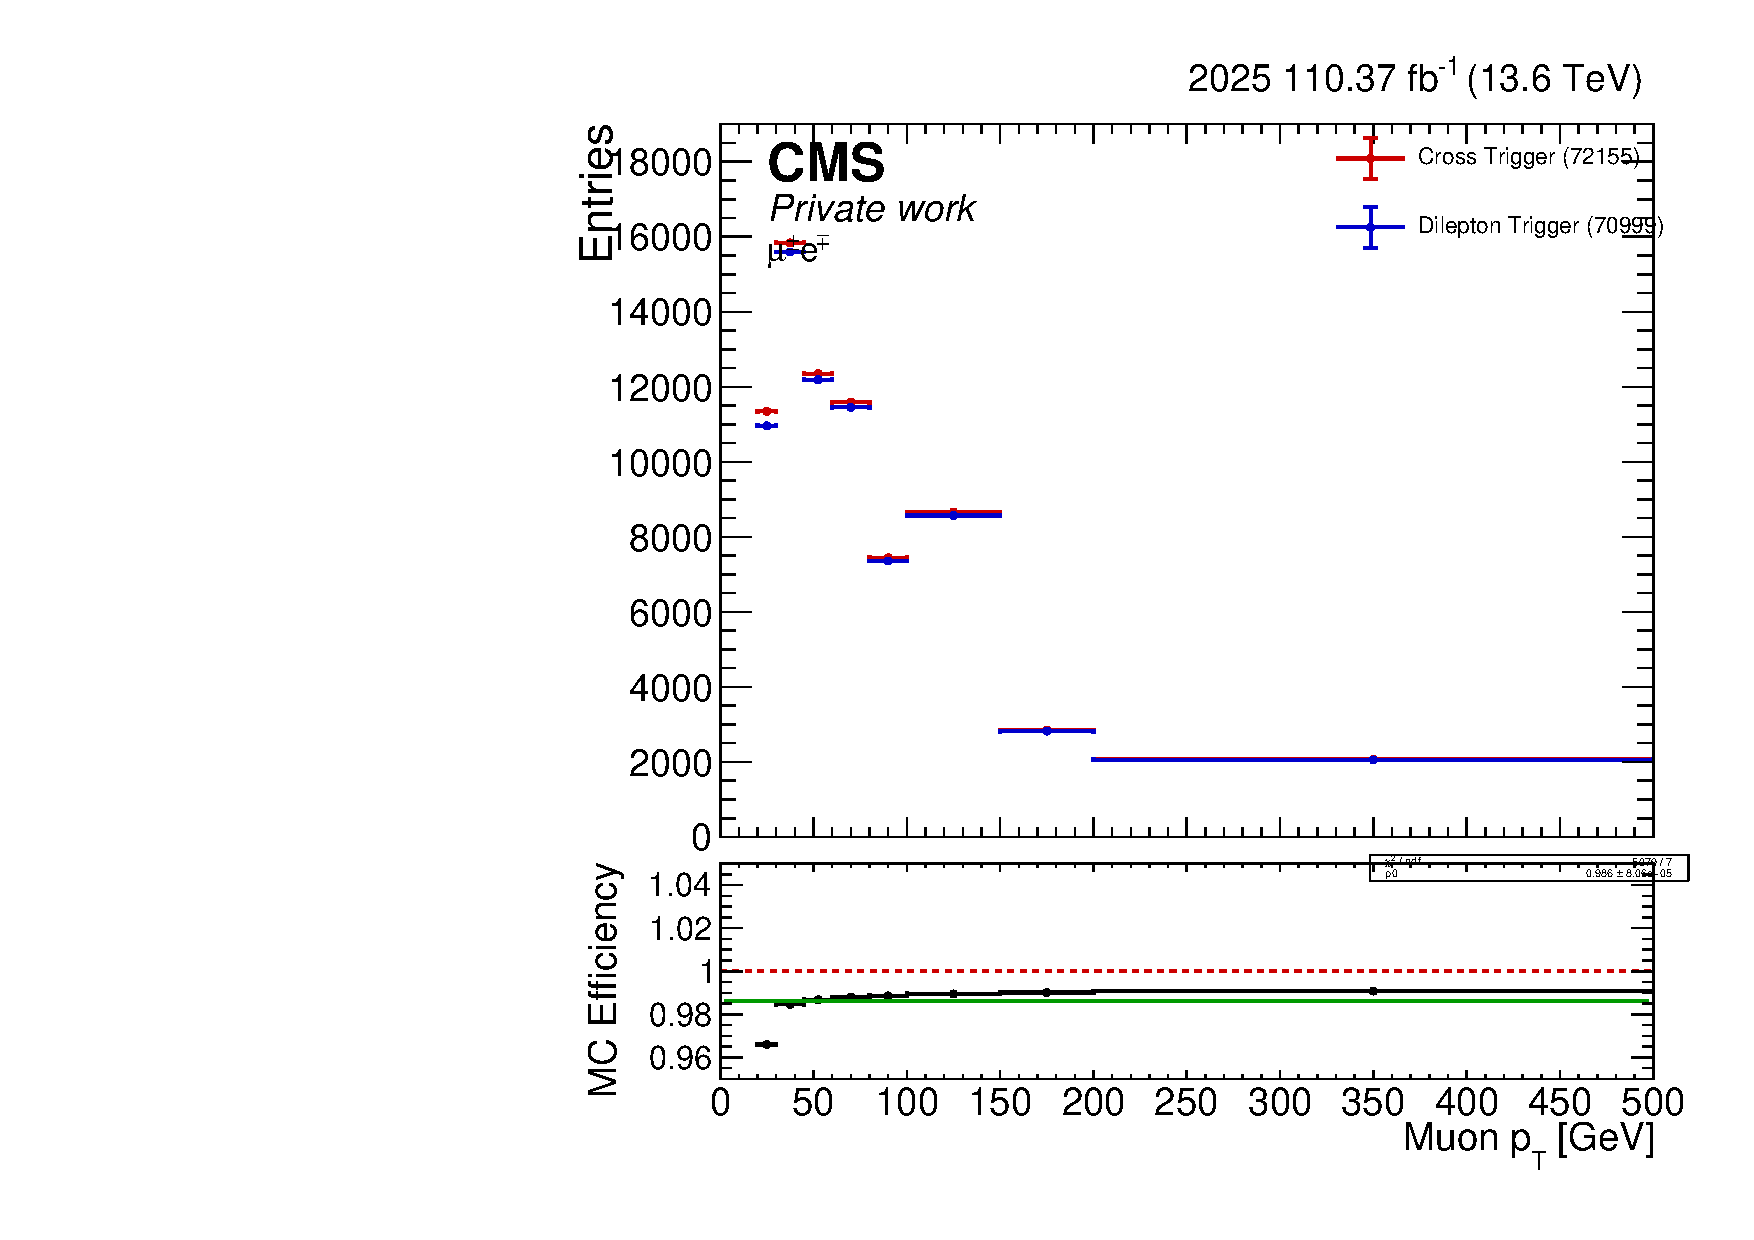
\includegraphics[width=0.48\linewidth]{figures/2025/MuEl/TrigEffMC/TrigEff_MuPt.pdf}
\caption{Simulated trigger numerator and reference-sample distributions (upper panels), with their efficiency ratios (lower panels) in the $e\mu$ channel. Left and right: electron and muon $p_{\mathrm{T}}$.}\label{fig:extra-MuEl-TrigEffMC-ElPt-2025}\end{figure}
\begin{figure}[p]\centering
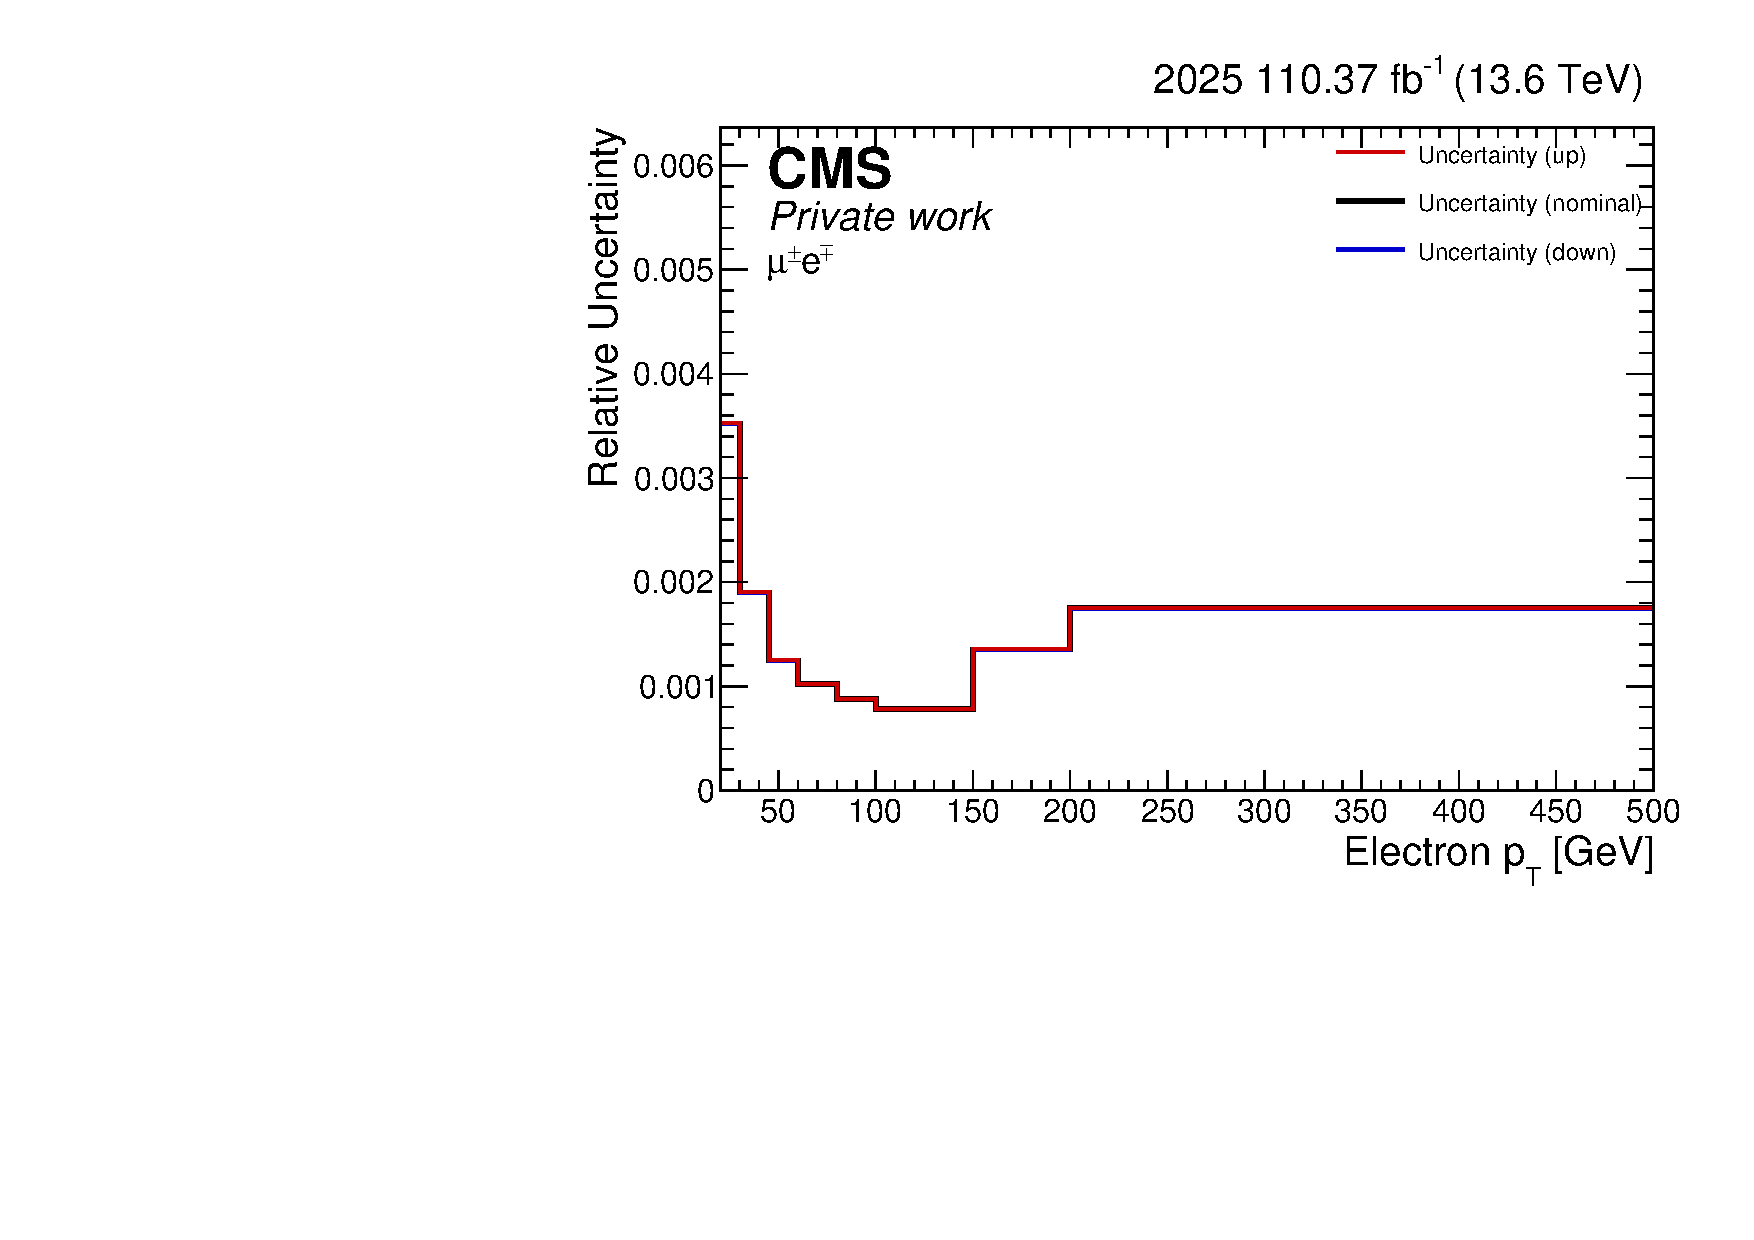
\includegraphics[width=0.48\linewidth]{figures/2025/MuEl/Statistical_Uncertainty/UncRatio_ElPt.pdf}
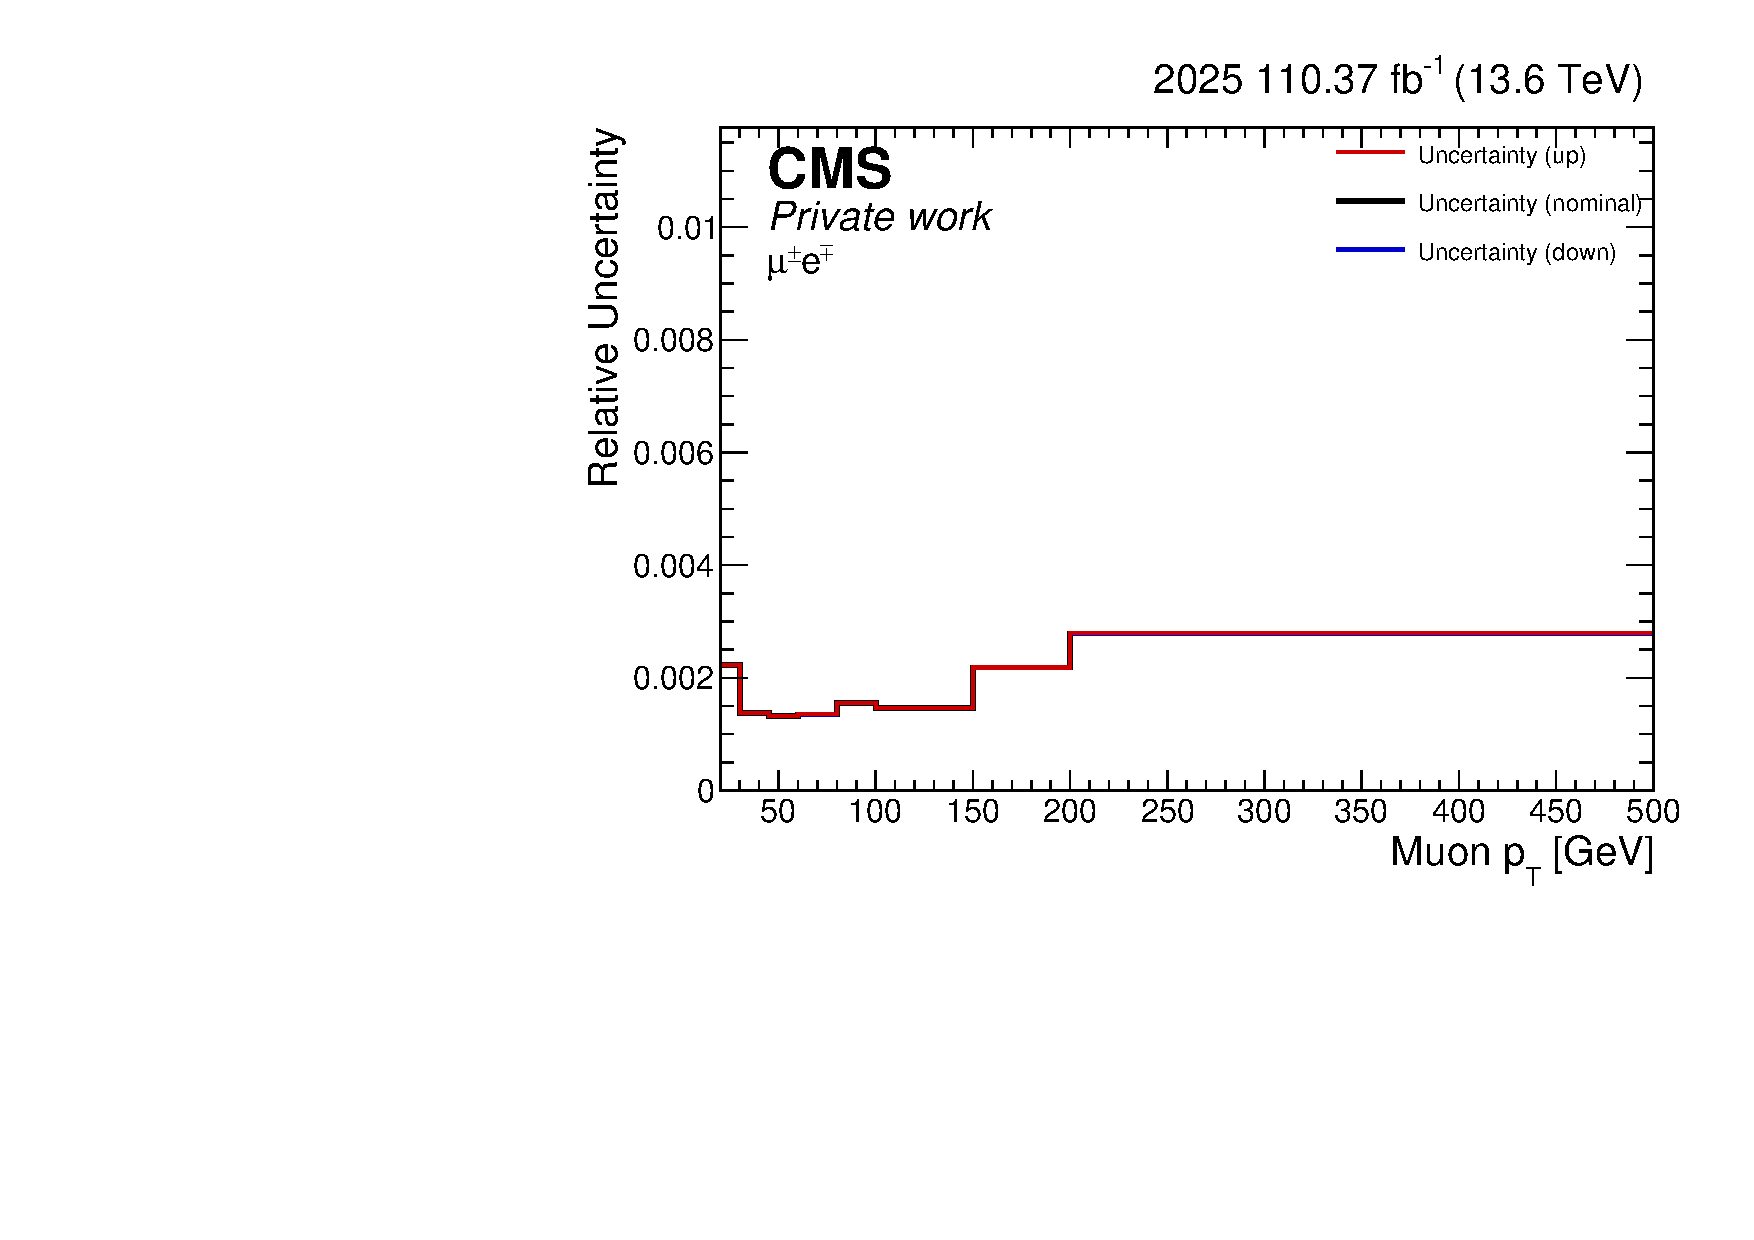
\includegraphics[width=0.48\linewidth]{figures/2025/MuEl/Statistical_Uncertainty/UncRatio_MuPt.pdf}
\caption{Relative statistical uncertainty diagnostics, retaining the nominal, upward, and downward curves of the supplied production in the $e\mu$ channel. Left and right: electron and muon $p_{\mathrm{T}}$.}\label{fig:extra-MuEl-Statistical-Uncertainty-ElPt-2025}\end{figure}
\begin{figure}[p]\centering
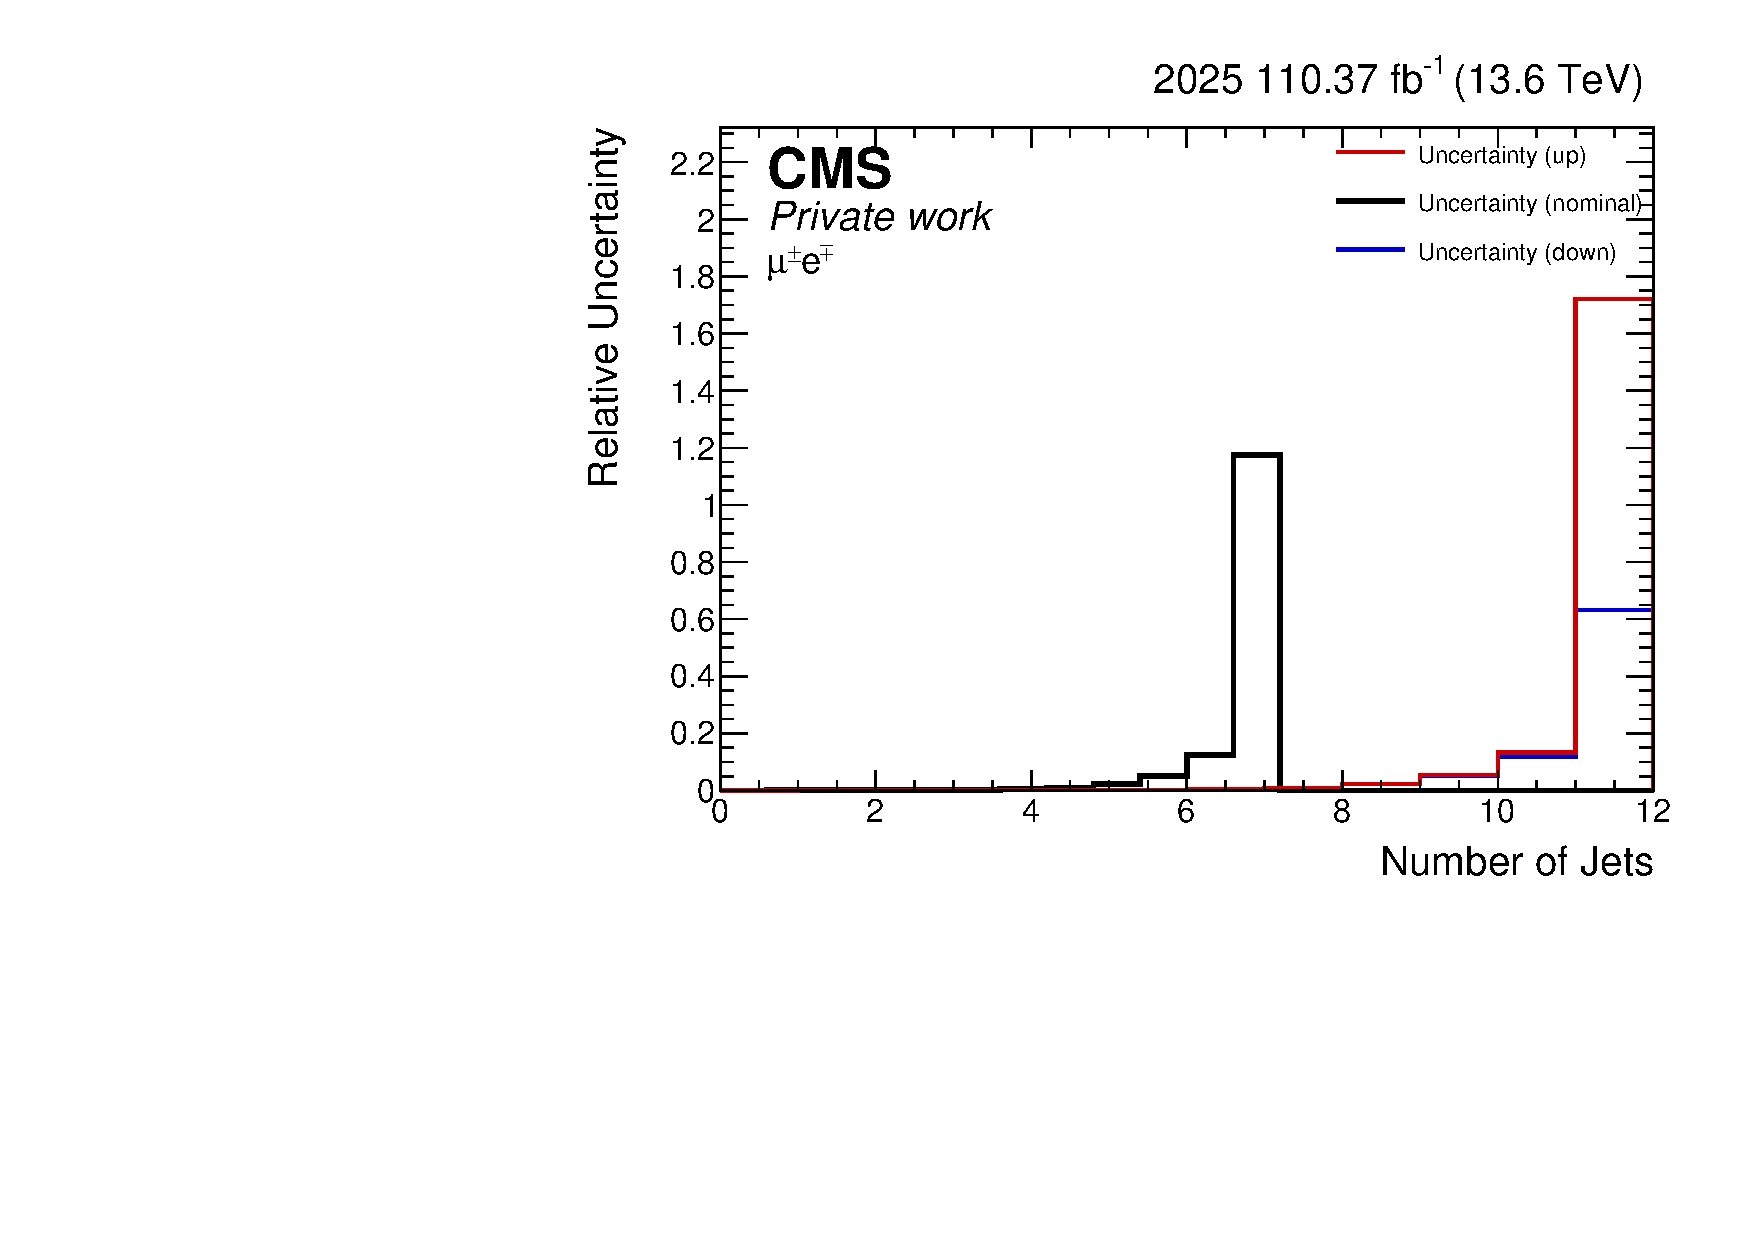
\includegraphics[width=0.48\linewidth]{figures/2025/MuEl/Statistical_Uncertainty/UncRatio_Num_Jets.pdf}
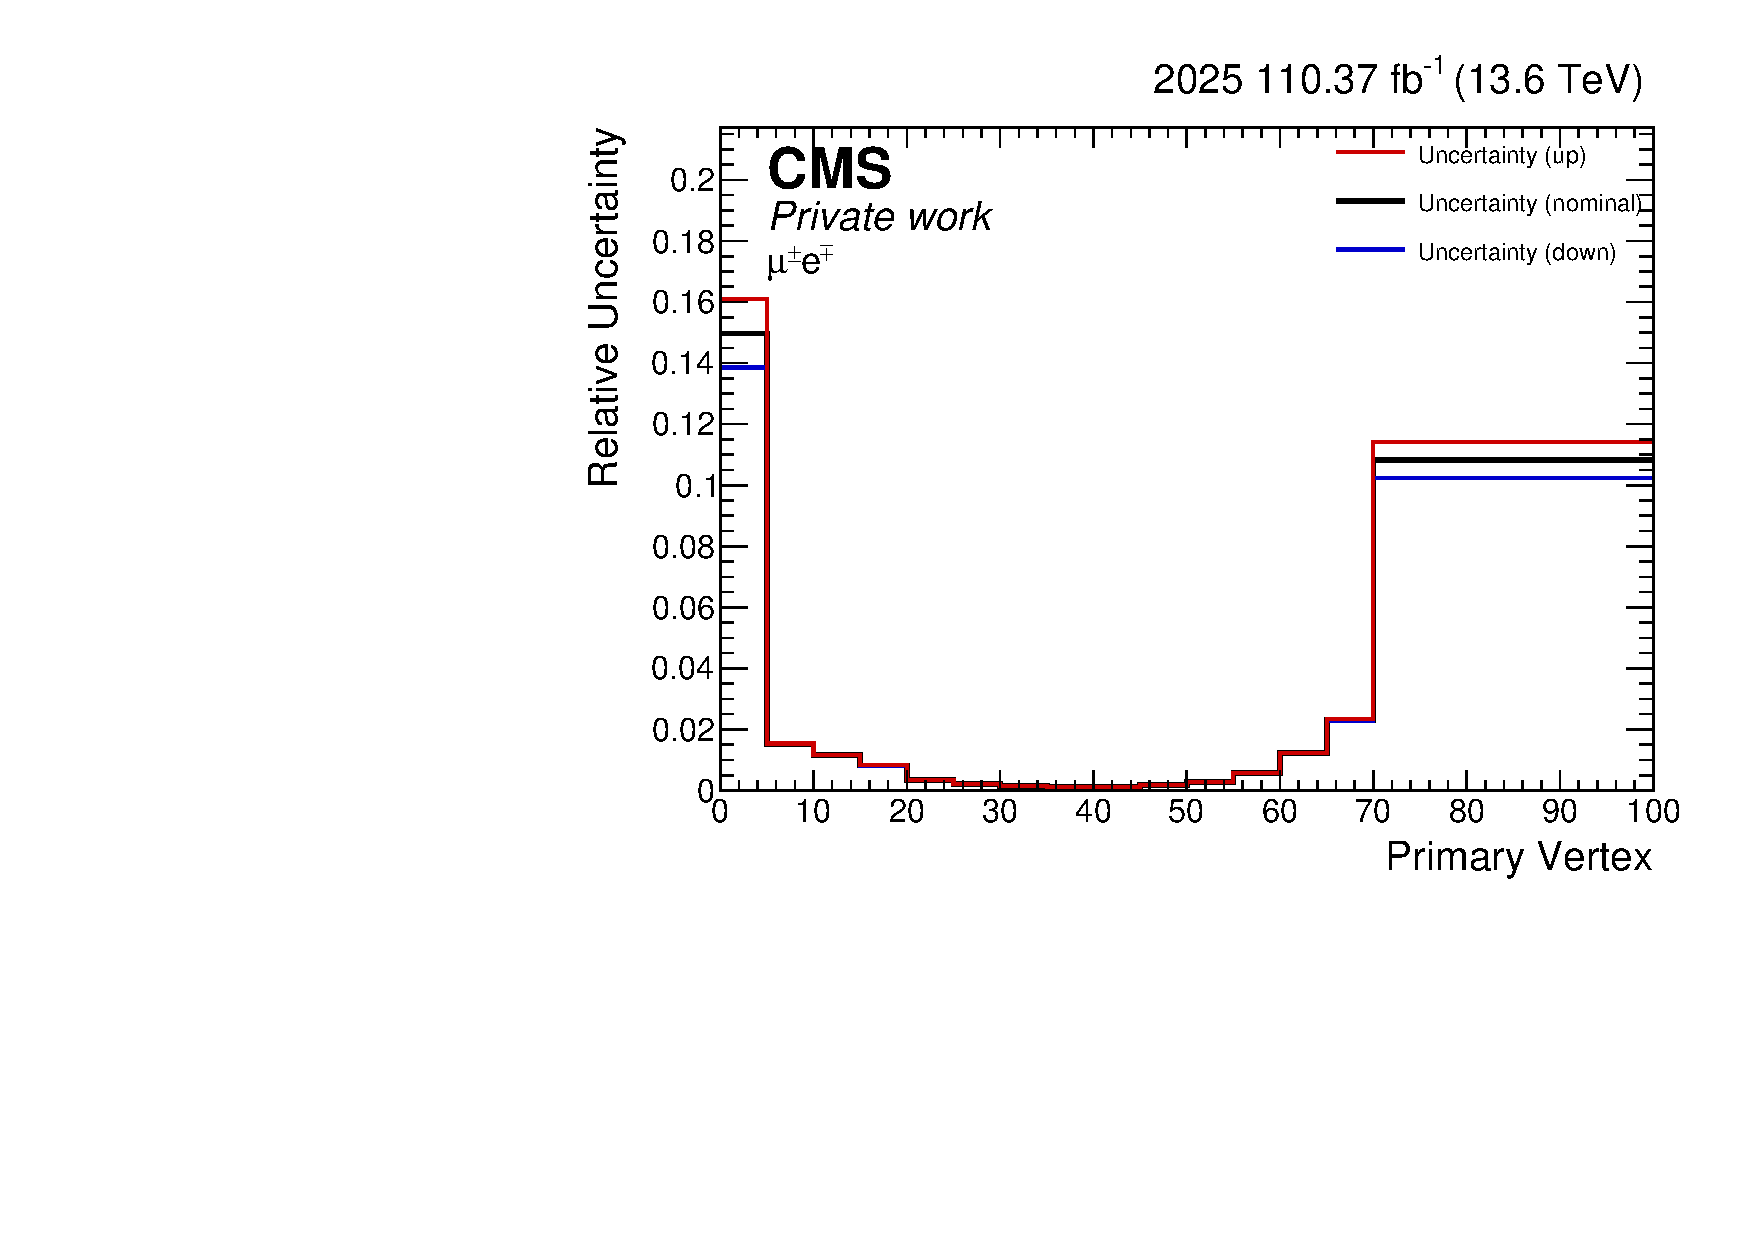
\includegraphics[width=0.48\linewidth]{figures/2025/MuEl/Statistical_Uncertainty/UncRatio_Num_PV.pdf}
\caption{Relative statistical uncertainty diagnostics, retaining the nominal, upward, and downward curves of the supplied production in the $e\mu$ channel. Left and right: jet and primary-vertex multiplicities.}\label{fig:extra-MuEl-Statistical-Uncertainty-Num_Jets-2025}\end{figure}
\begin{figure}[p]\centering
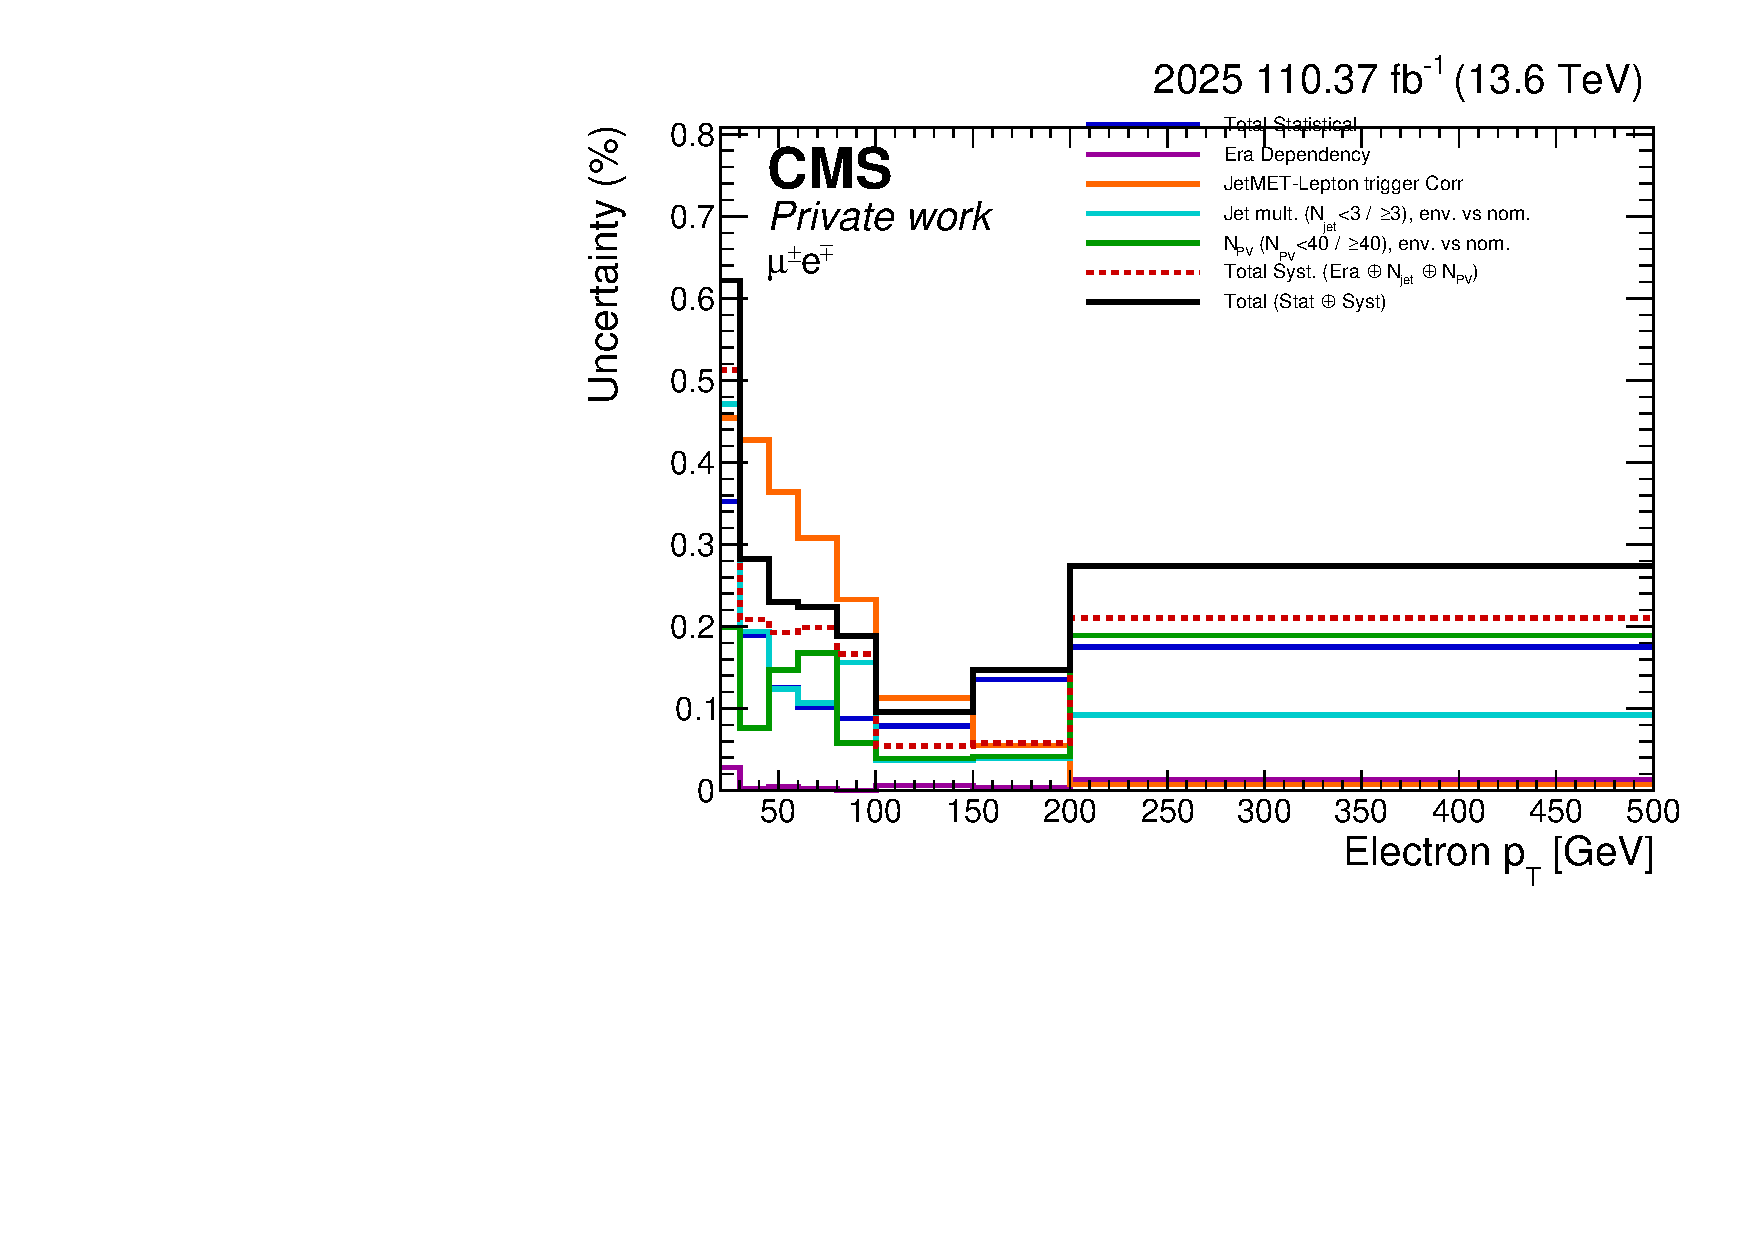
\includegraphics[width=0.48\linewidth]{figures/2025/MuEl/Uncertainty_Breakdown/Breakdown_ElPt.pdf}
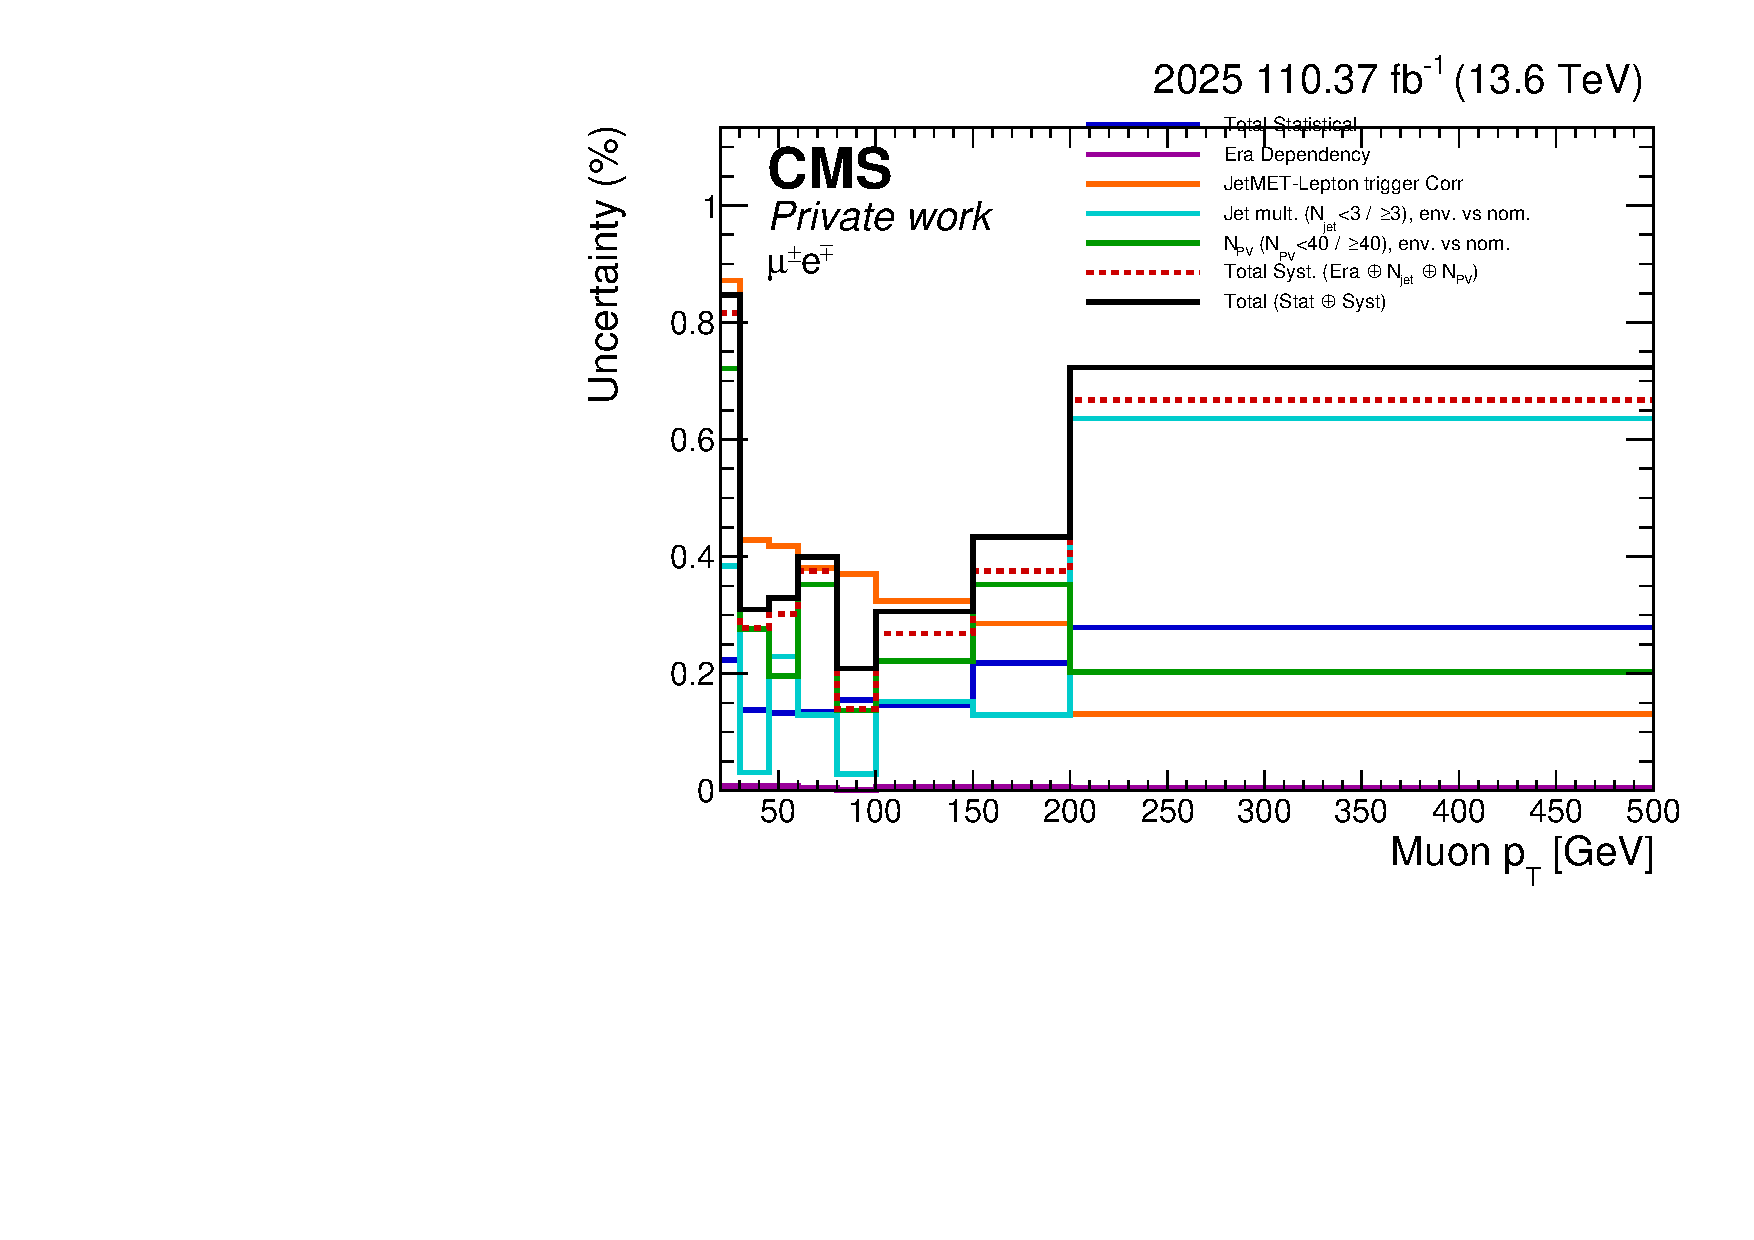
\includegraphics[width=0.48\linewidth]{figures/2025/MuEl/Uncertainty_Breakdown/Breakdown_MuPt.pdf}
\caption{Absolute uncertainty component breakdown in the $e\mu$ channel. Left and right: electron and muon $p_{\mathrm{T}}$.}\label{fig:extra-MuEl-Uncertainty-Breakdown-ElPt-2025}\end{figure}
\begin{figure}[p]\centering
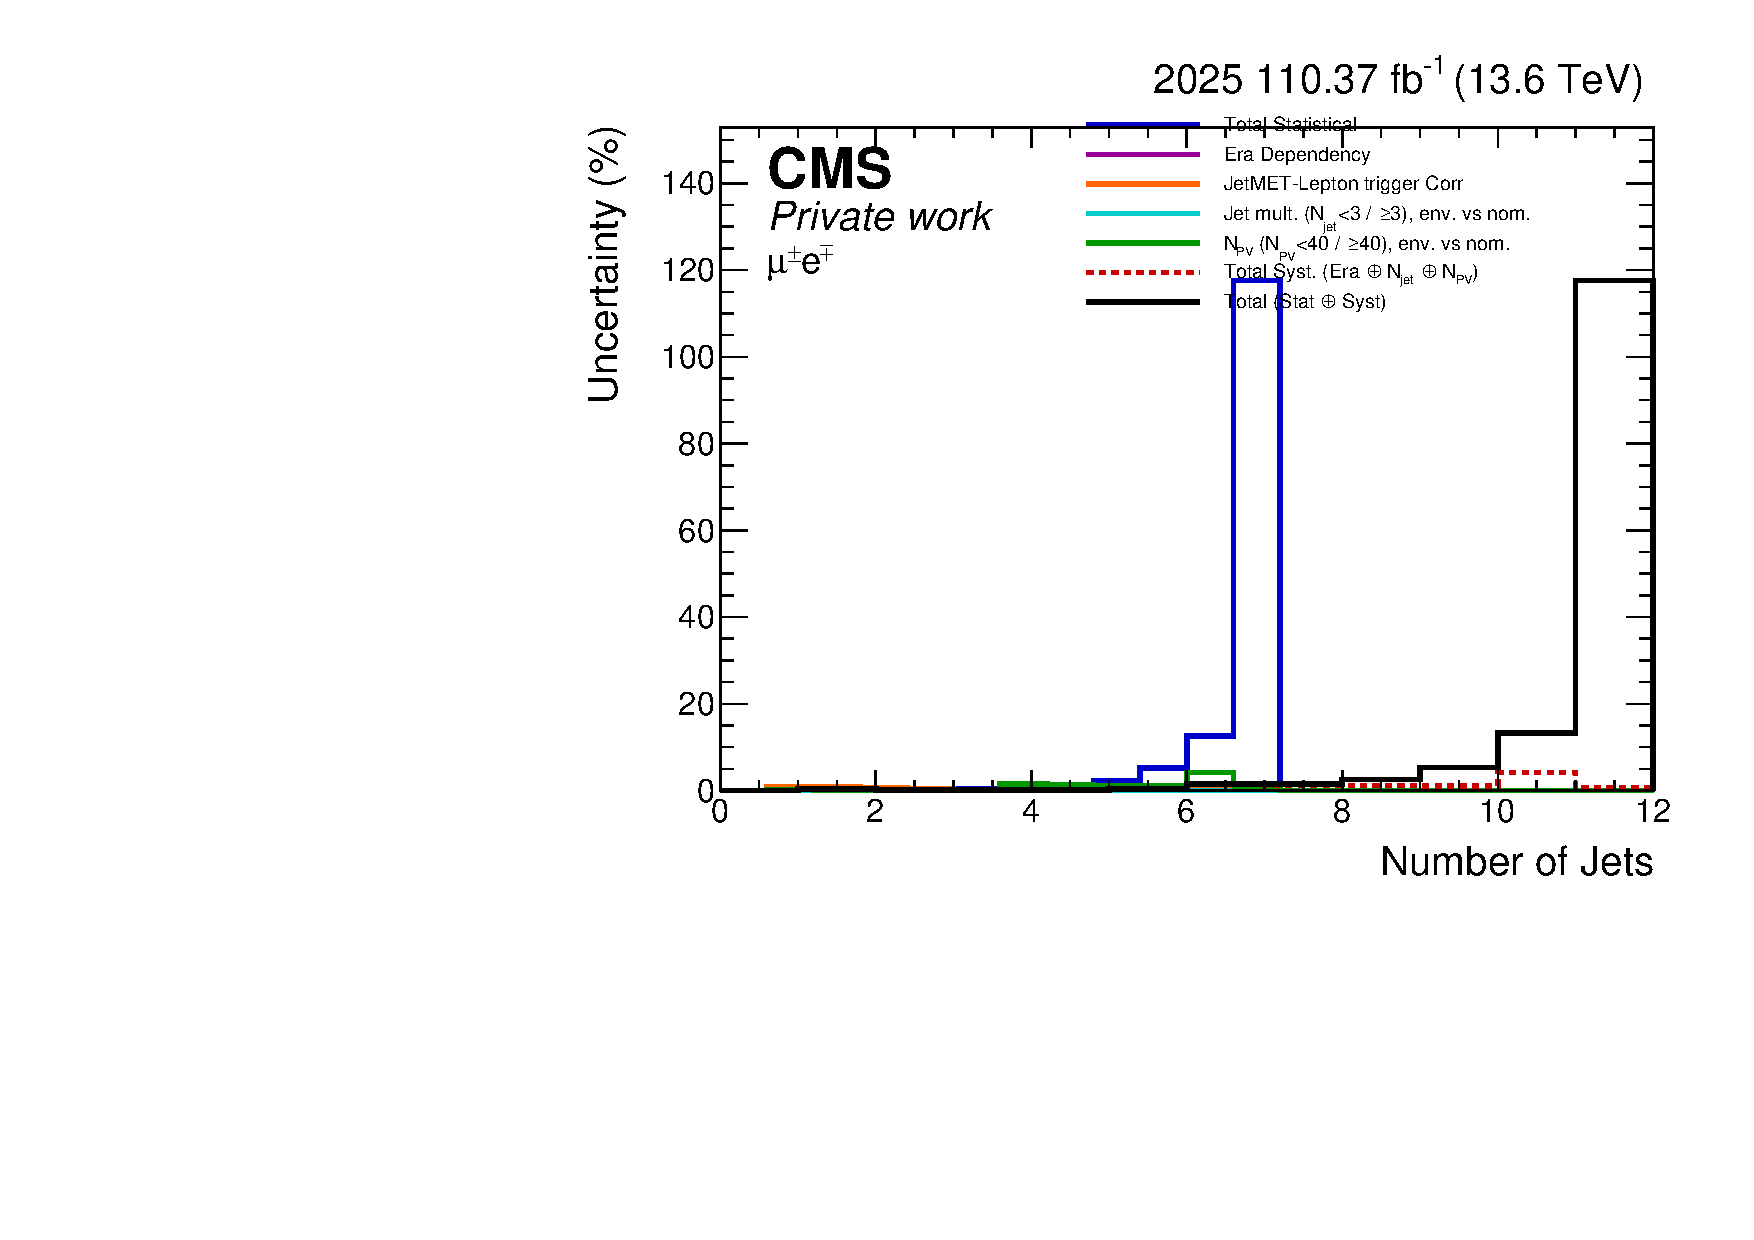
\includegraphics[width=0.48\linewidth]{figures/2025/MuEl/Uncertainty_Breakdown/Breakdown_Num_Jets.pdf}
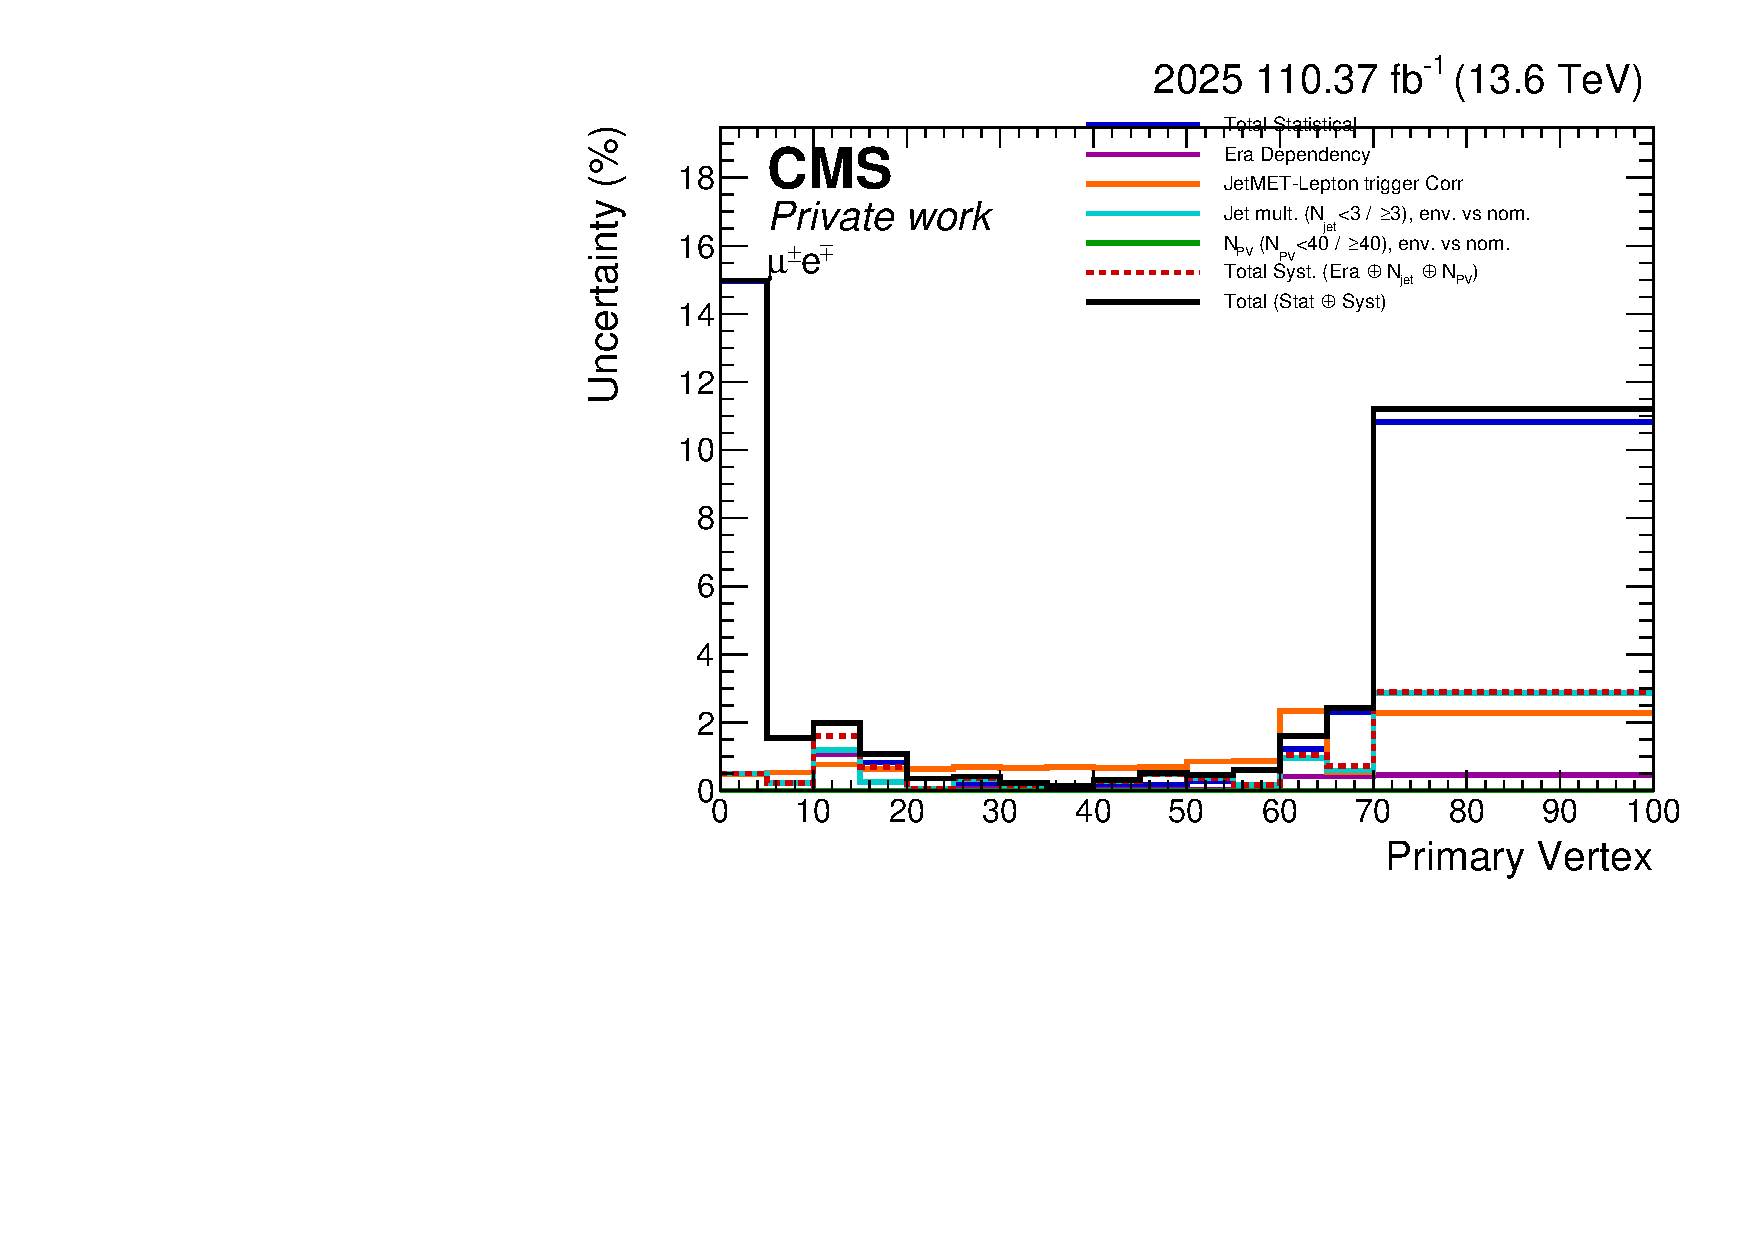
\includegraphics[width=0.48\linewidth]{figures/2025/MuEl/Uncertainty_Breakdown/Breakdown_Num_PV.pdf}
\caption{Absolute uncertainty component breakdown in the $e\mu$ channel. Left and right: jet and primary-vertex multiplicities.}\label{fig:extra-MuEl-Uncertainty-Breakdown-Num_Jets-2025}\end{figure}
\begin{figure}[p]\centering
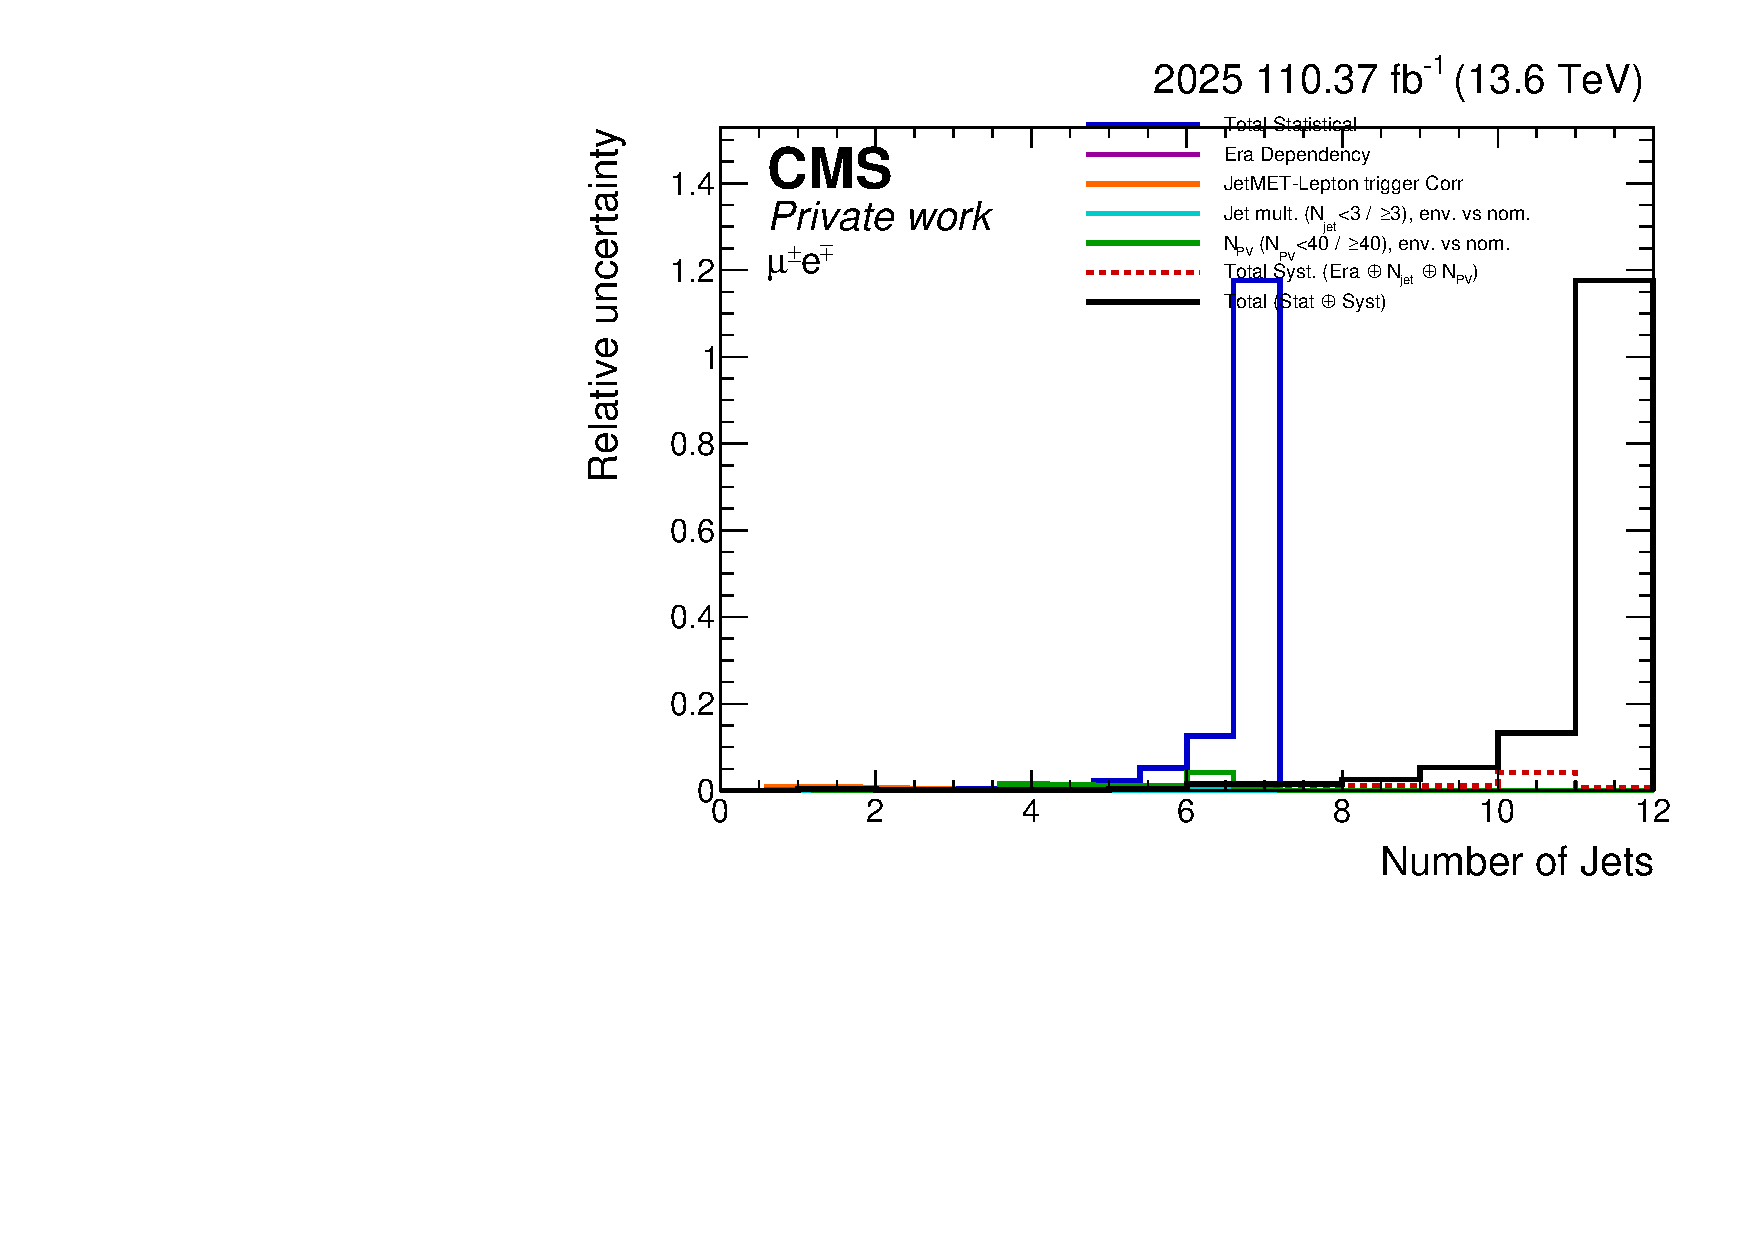
\includegraphics[width=0.48\linewidth]{figures/2025/MuEl/Relative_Uncertainty_Breakdown/Breakdown_Num_Jets.pdf}
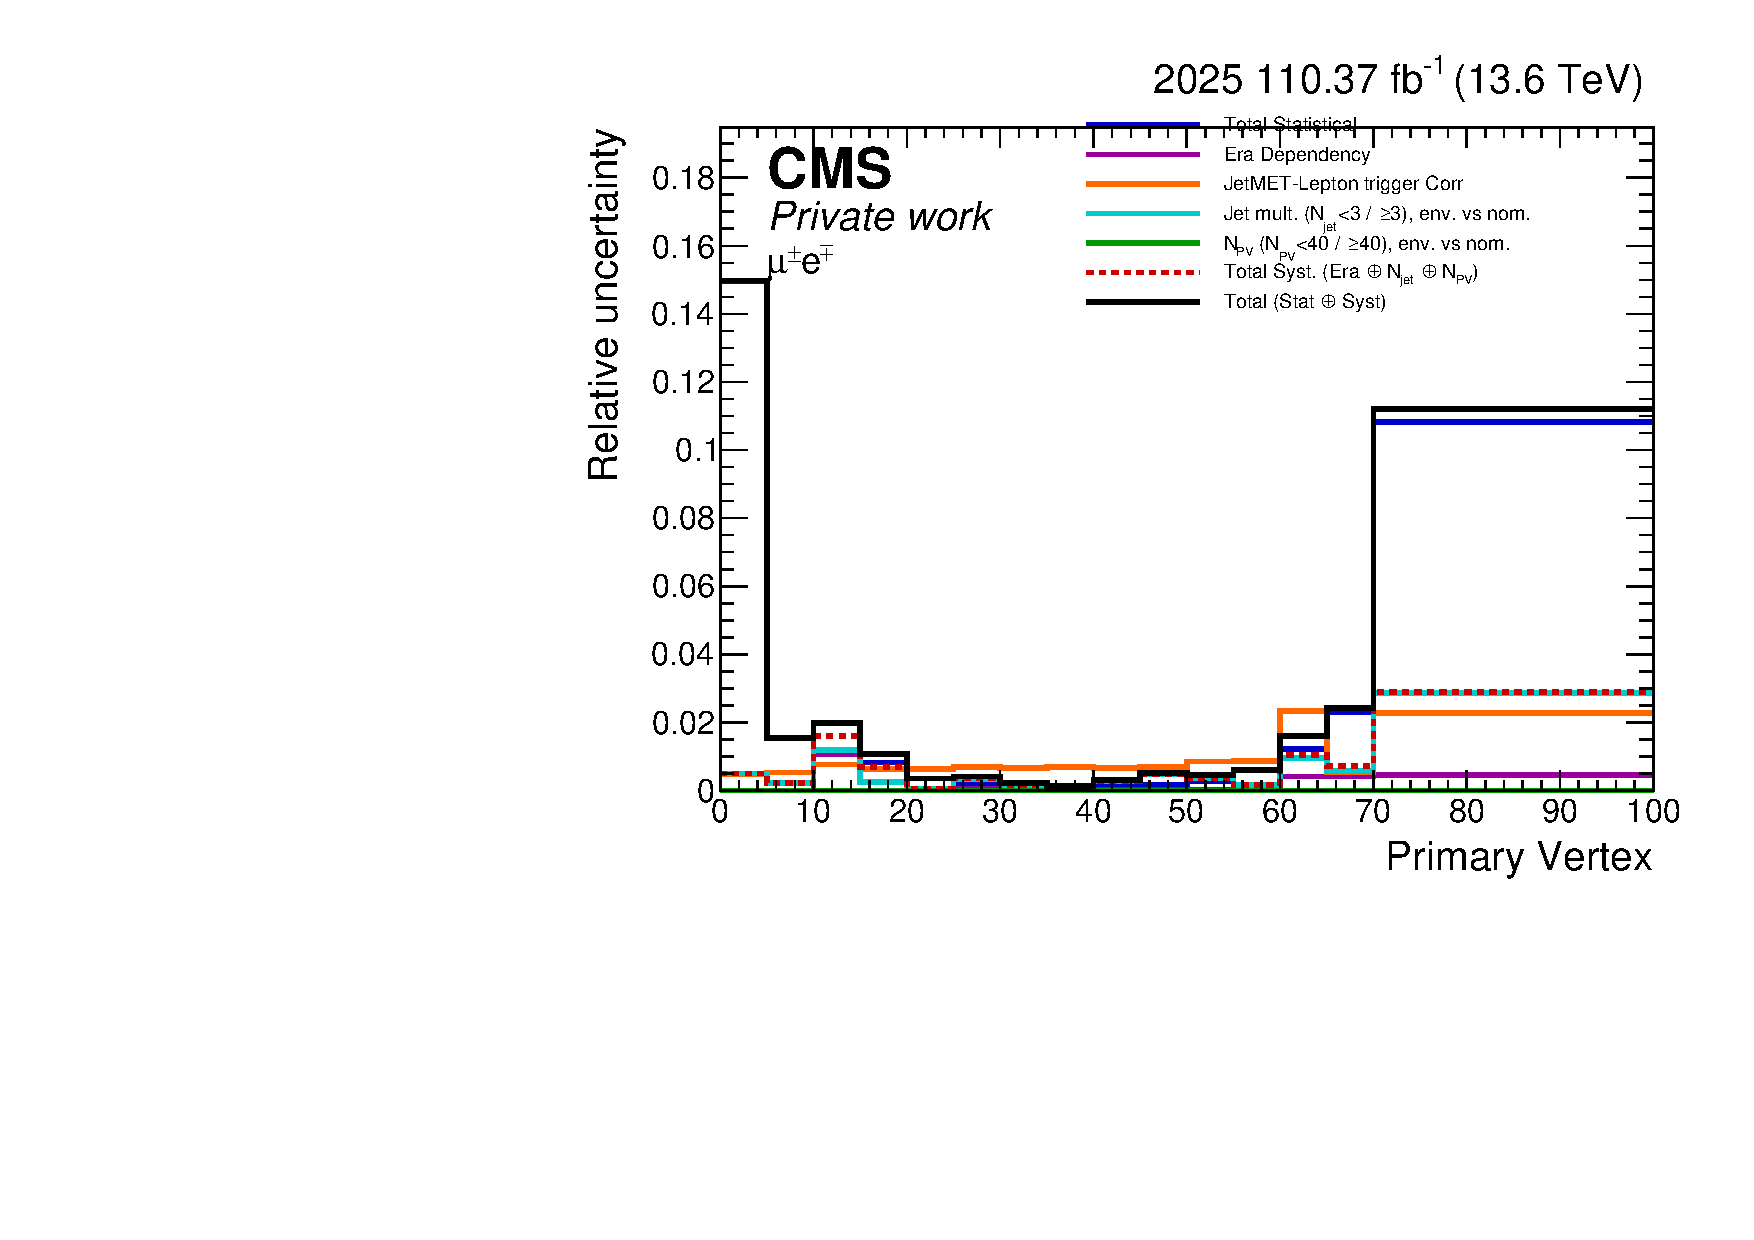
\includegraphics[width=0.48\linewidth]{figures/2025/MuEl/Relative_Uncertainty_Breakdown/Breakdown_Num_PV.pdf}
\caption{Relative uncertainty component breakdown versus event activity in the $e\mu$ channel. Left and right: jet and primary-vertex multiplicities.}\label{fig:extra-MuEl-Relative-Uncertainty-Breakdown-Num_Jets-2025}\end{figure}
\begin{figure}[p]\centering
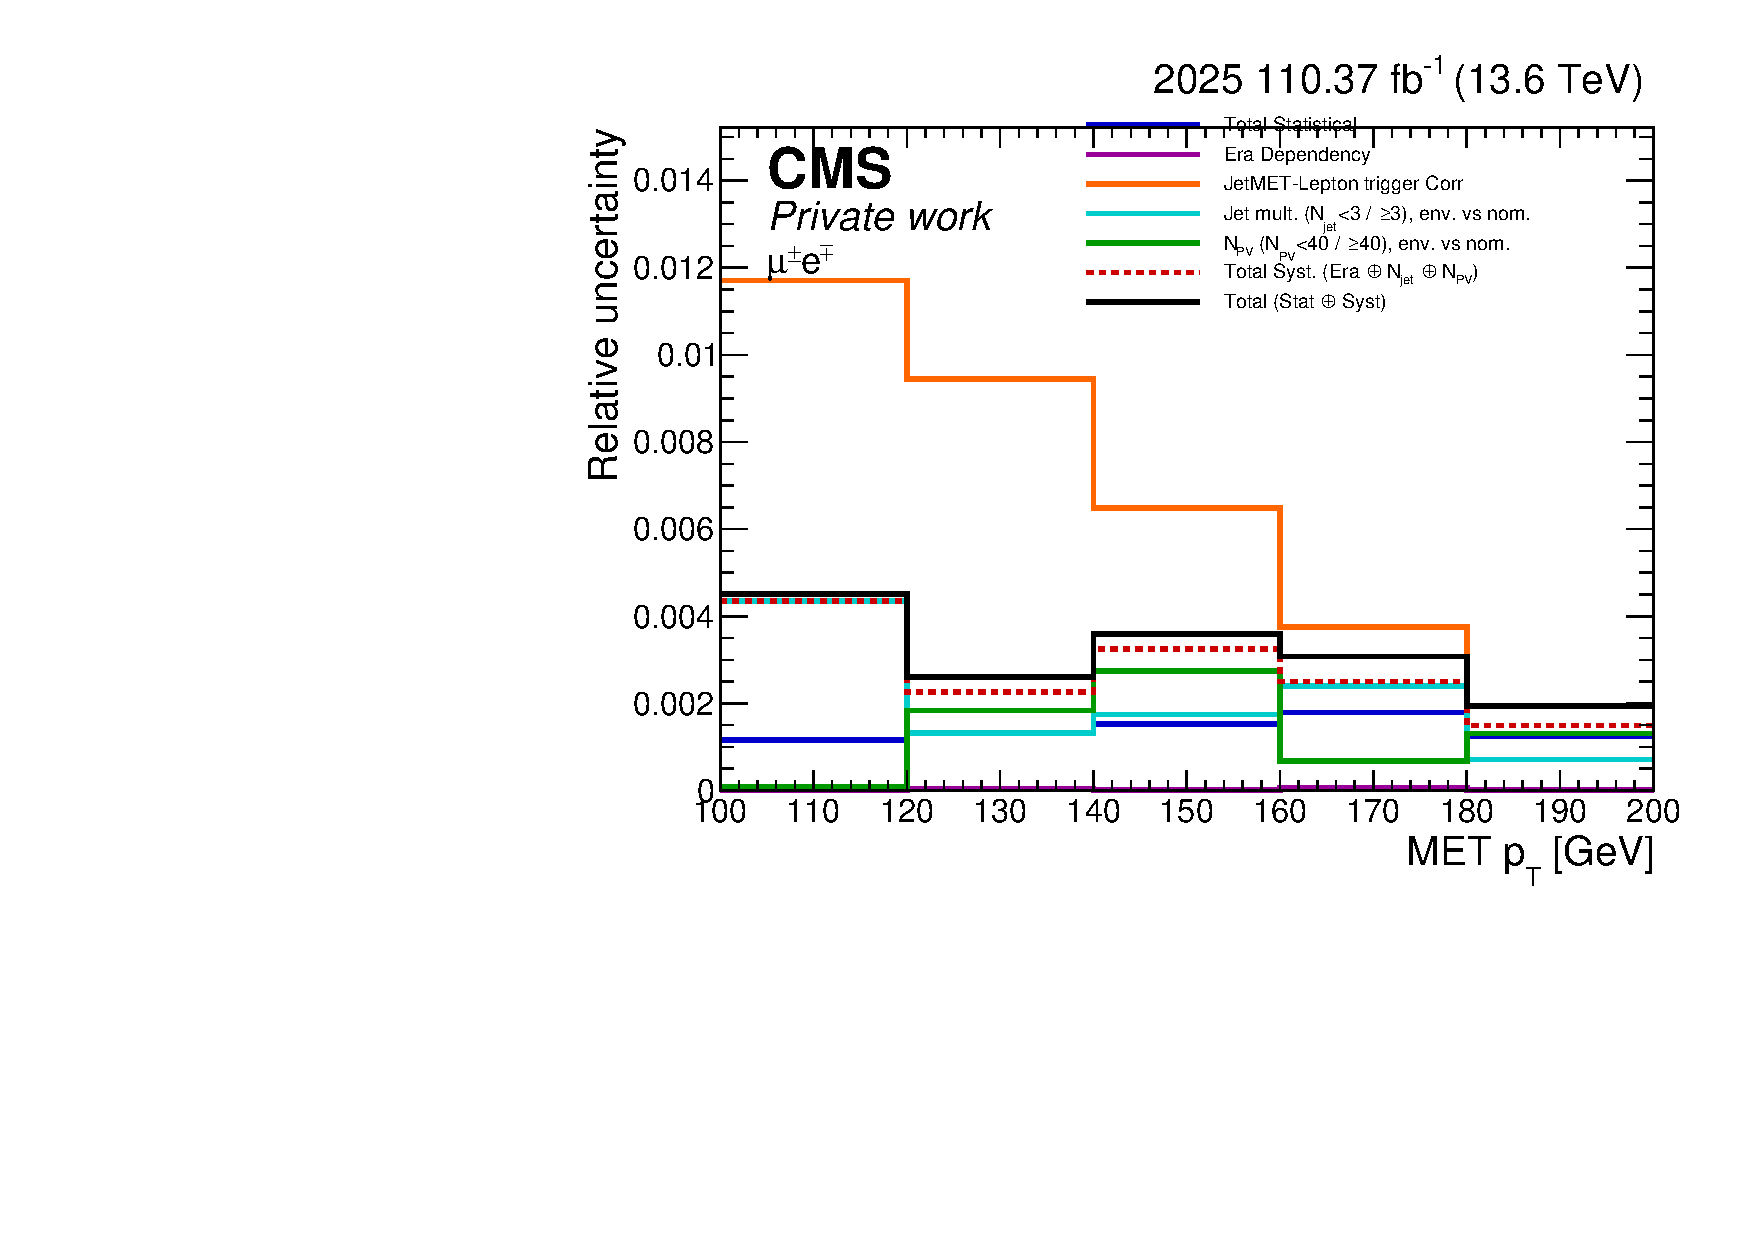
\includegraphics[width=0.48\linewidth]{figures/2025/MuEl/Relative_Uncertainty_Breakdown/Breakdown_METpt.pdf}
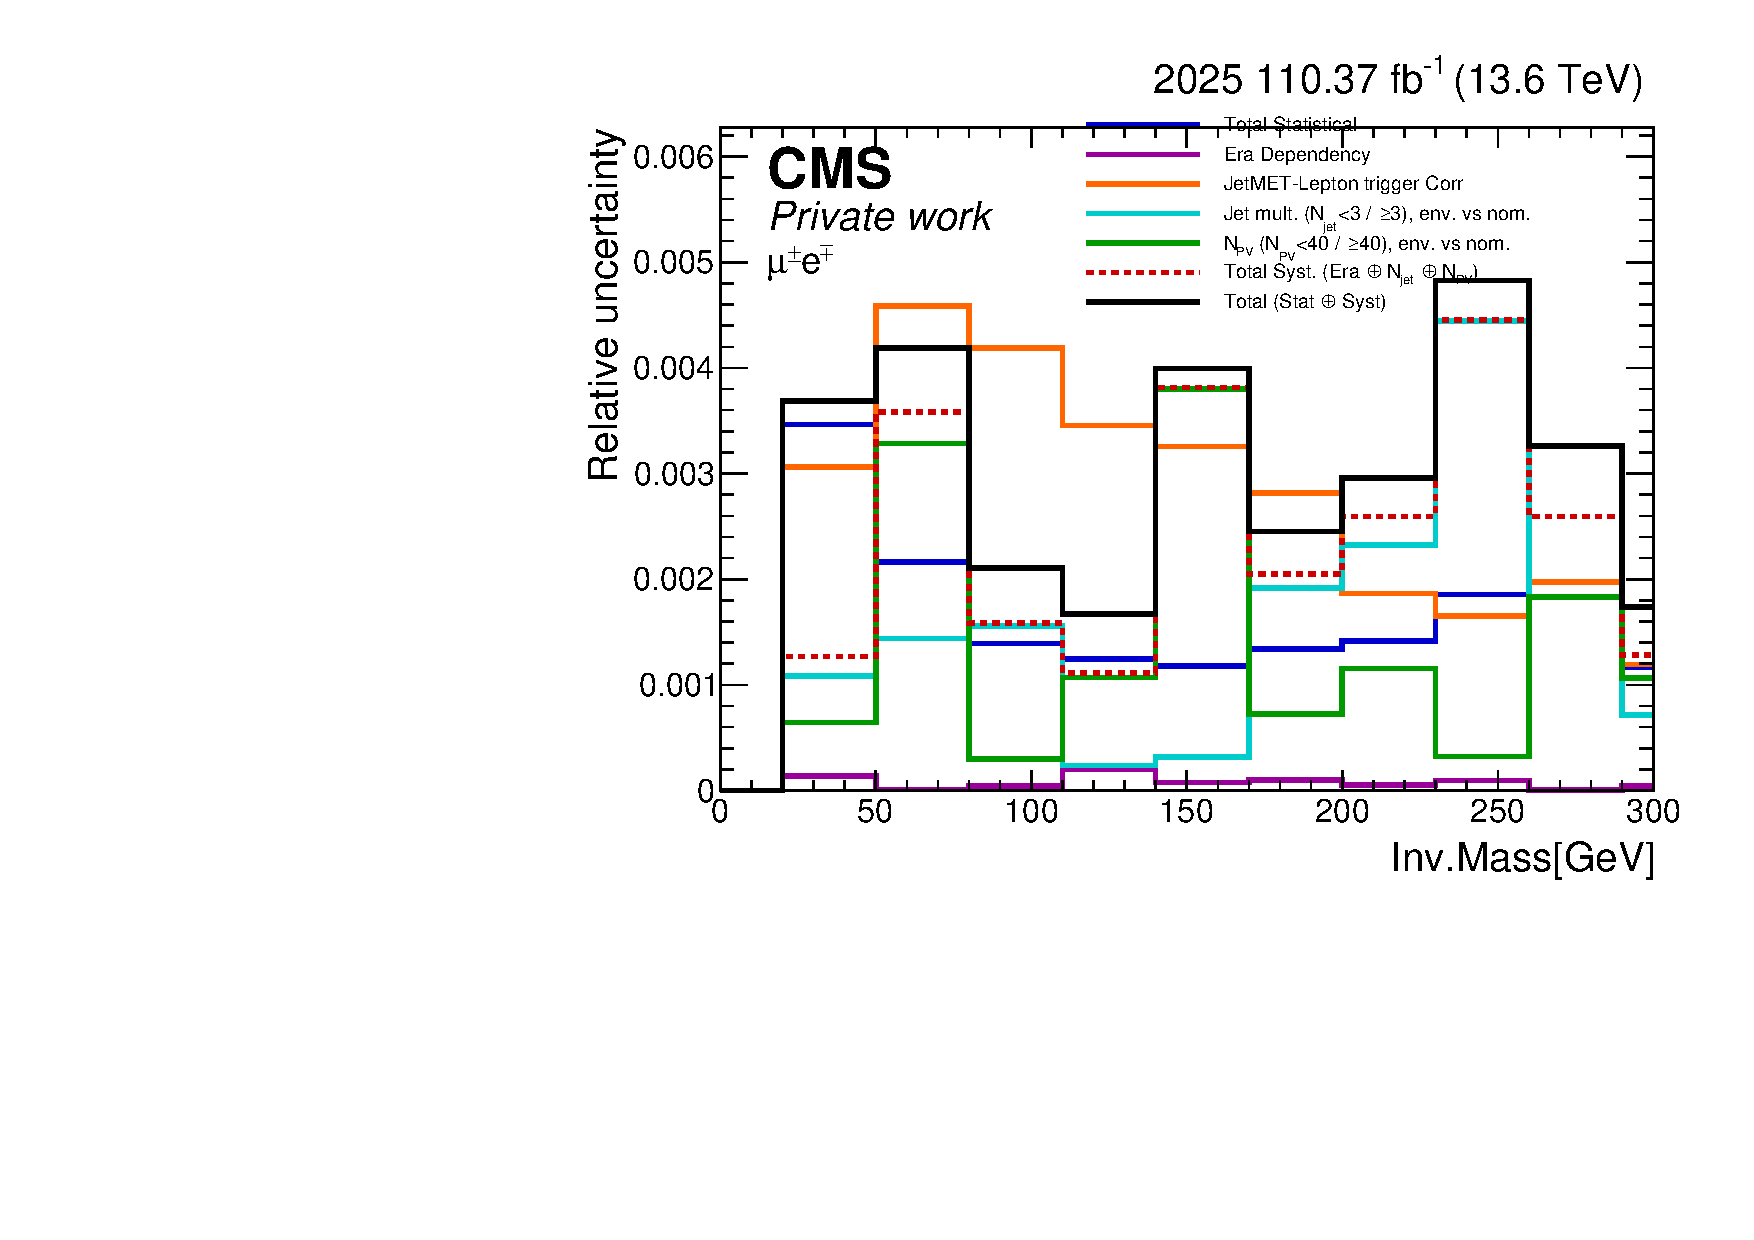
\includegraphics[width=0.48\linewidth]{figures/2025/MuEl/Relative_Uncertainty_Breakdown/Breakdown_DiLepMass.pdf}
\caption{Relative uncertainty component breakdown versus event kinematics in the $e\mu$ channel. Left and right: missing transverse momentum and dilepton invariant mass.}\label{fig:extra-MuEl-Relative-Uncertainty-Breakdown-METpt-2025}\end{figure}
\begin{figure}[p]\centering
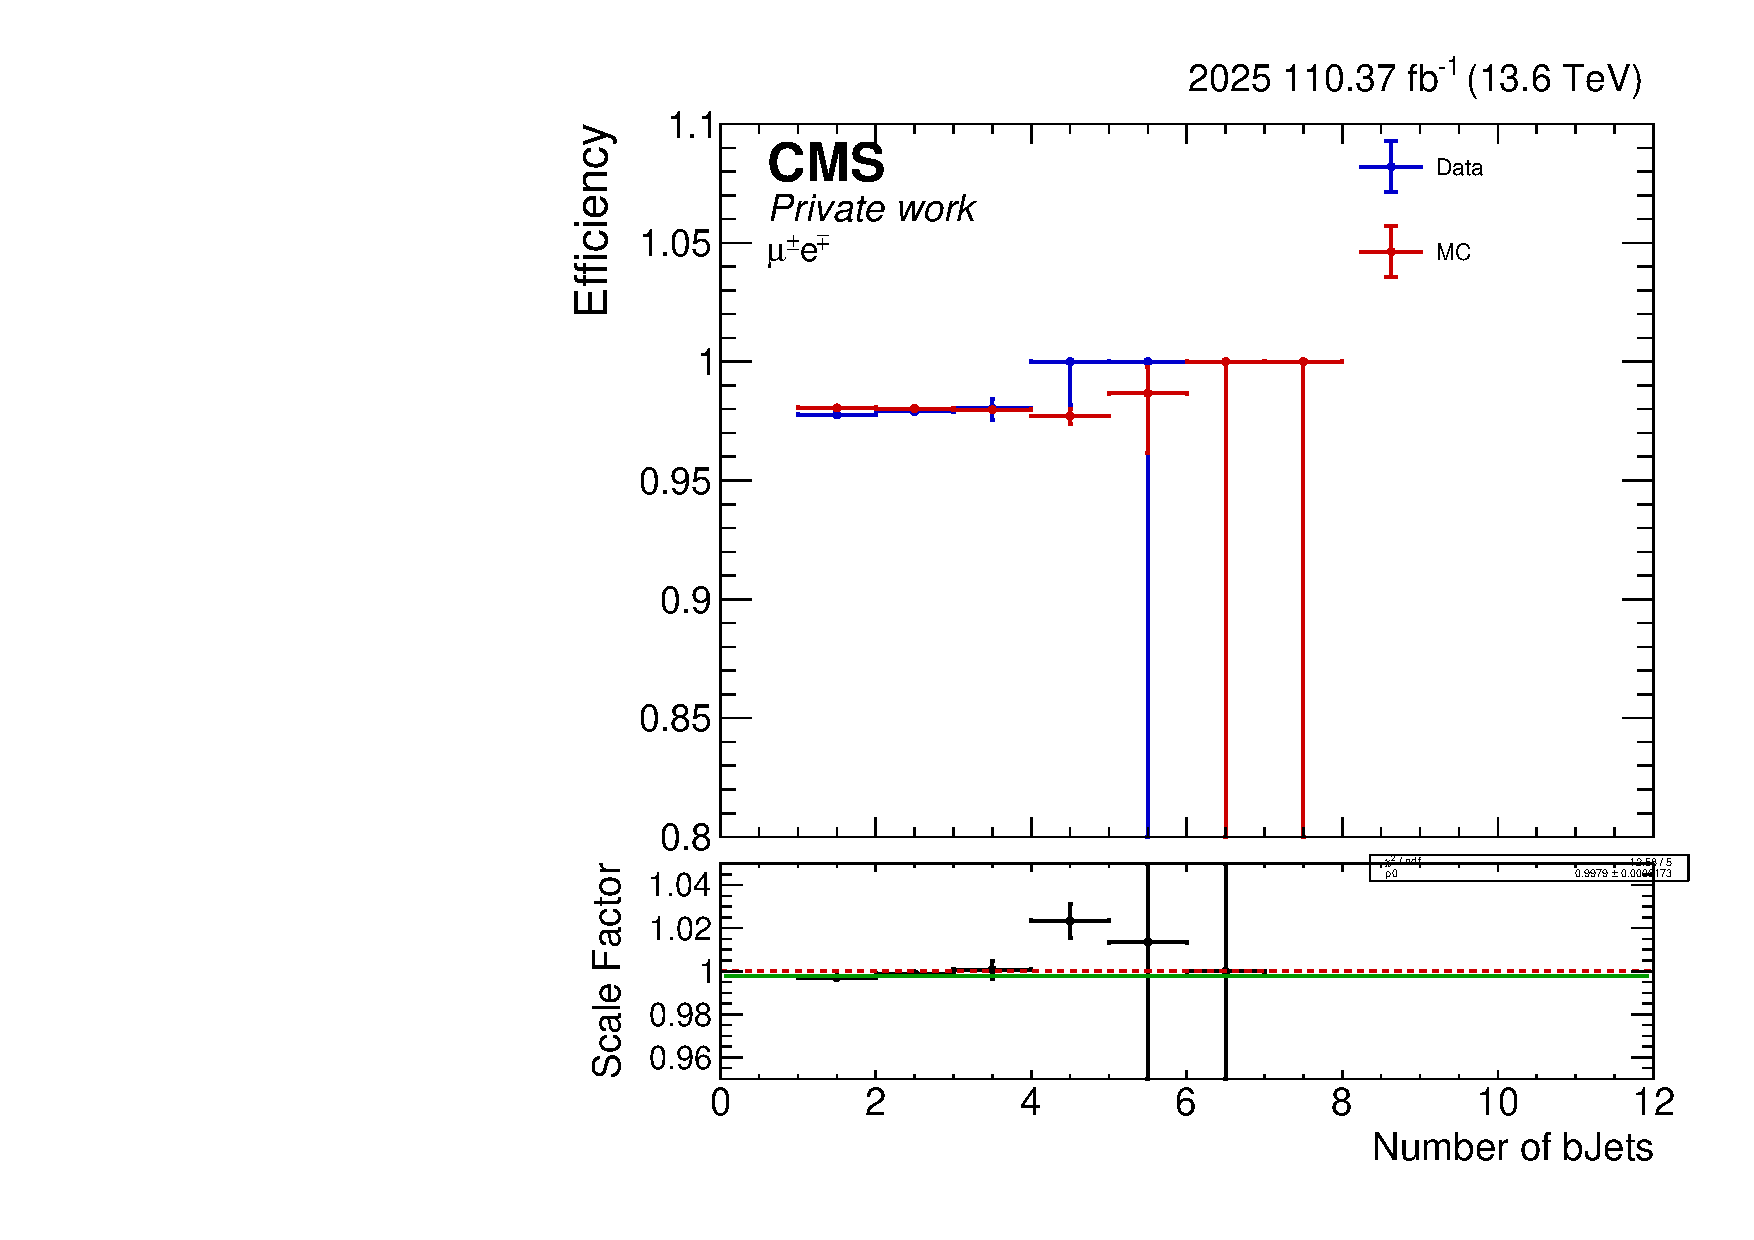
\includegraphics[width=0.48\linewidth]{figures/2025/MuEl/ScaleFactor/SF_Num_bJets.pdf}
\caption{Efficiency comparison and scale factor versus heavy-flavour activity in the $e\mu$ channel. $b$-tagged jet multiplicity.}\label{fig:extra-MuEl-ScaleFactor-Num_bJets-2025}\end{figure}
\begin{figure}[p]\centering
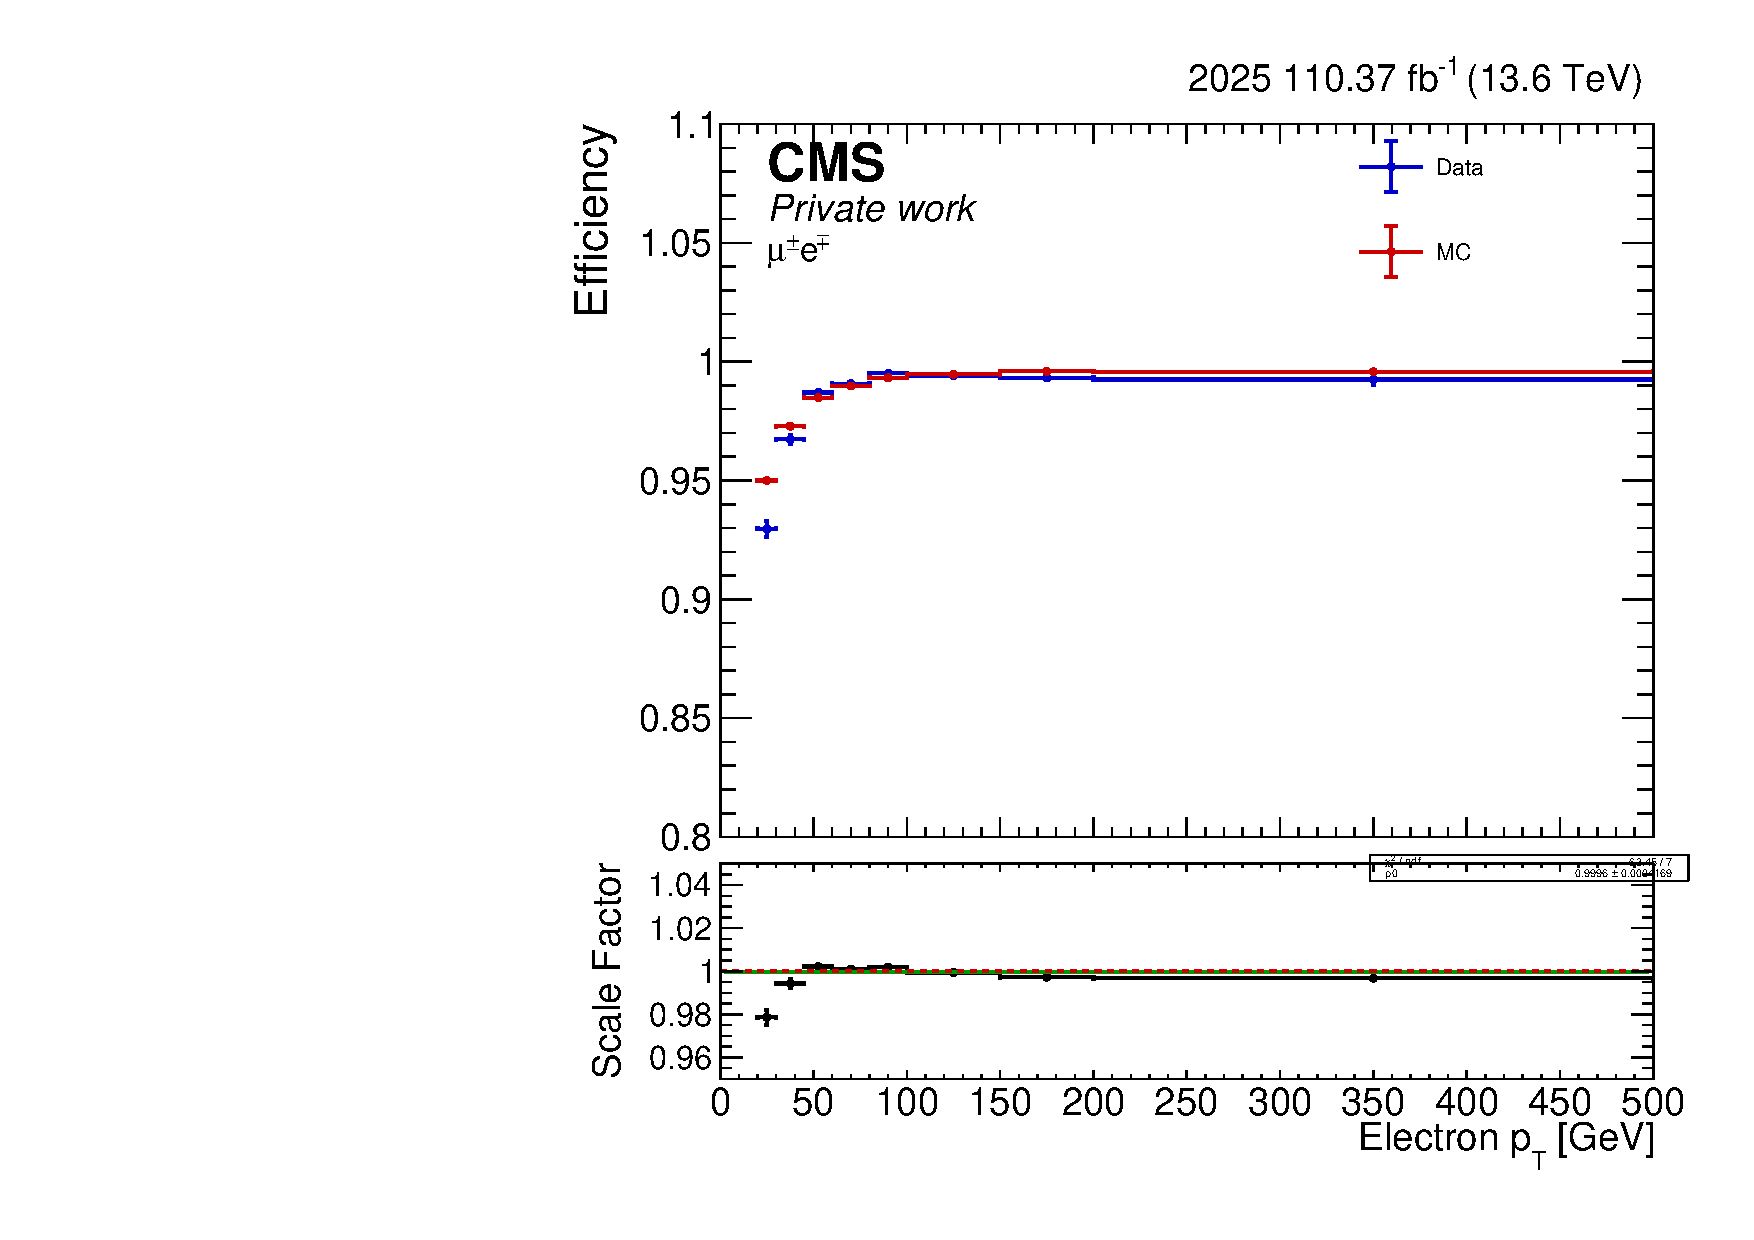
\includegraphics[width=0.48\linewidth]{figures/2025/MuEl/ScaleFactor/SF_ElPt.pdf}
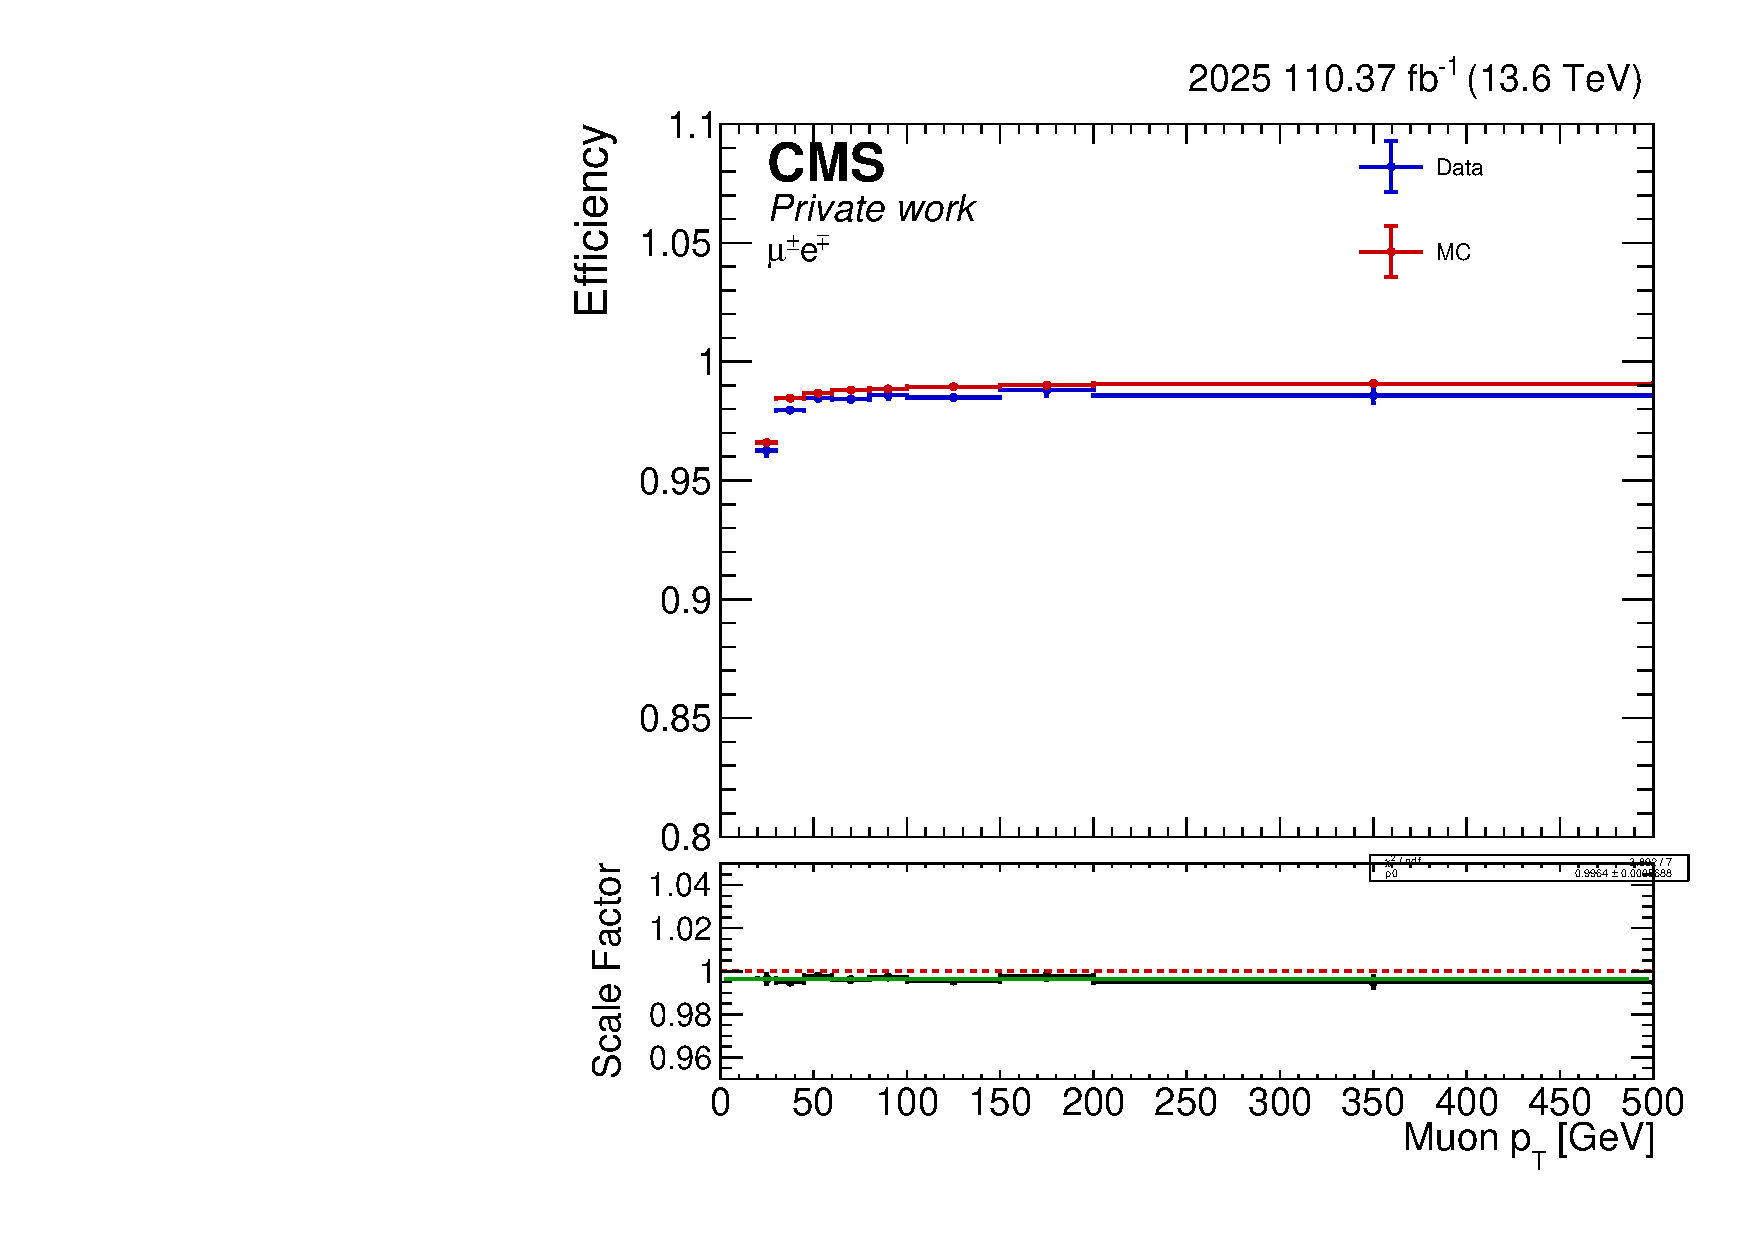
\includegraphics[width=0.48\linewidth]{figures/2025/MuEl/ScaleFactor/SF_MuPt.pdf}
\caption{Efficiency comparison and scale factor in the flavour-specific momentum variables used by the two-dimensional correction in the $e\mu$ channel. Left and right: electron and muon $p_{\mathrm{T}}$.}\label{fig:extra-MuEl-ScaleFactor-ElPt-2025}\end{figure}
\clearpage\subsection{$\mu\mu$ channel}
\begin{figure}[p]\centering
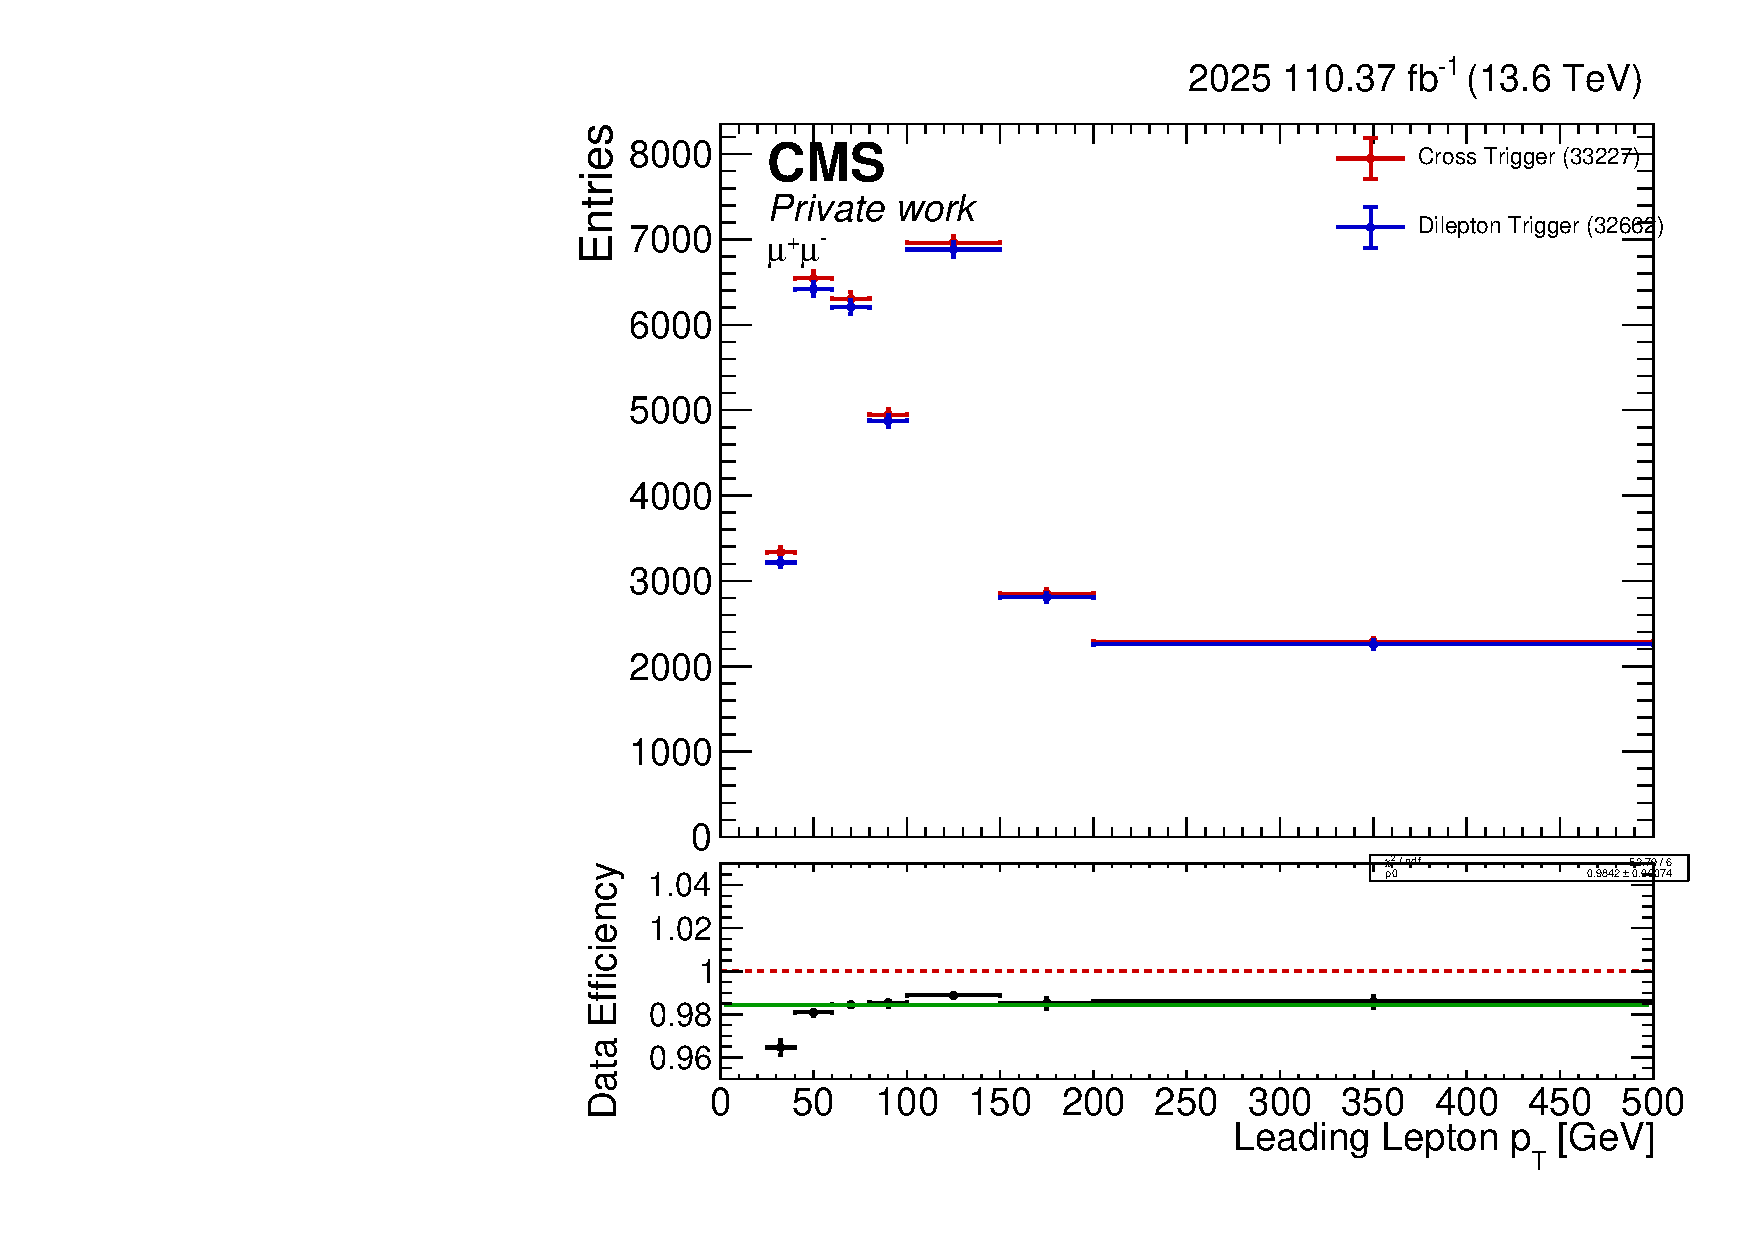
\includegraphics[width=0.48\linewidth]{figures/2025/MuMu/TrigEffData/TrigEff_Lep1pt.pdf}
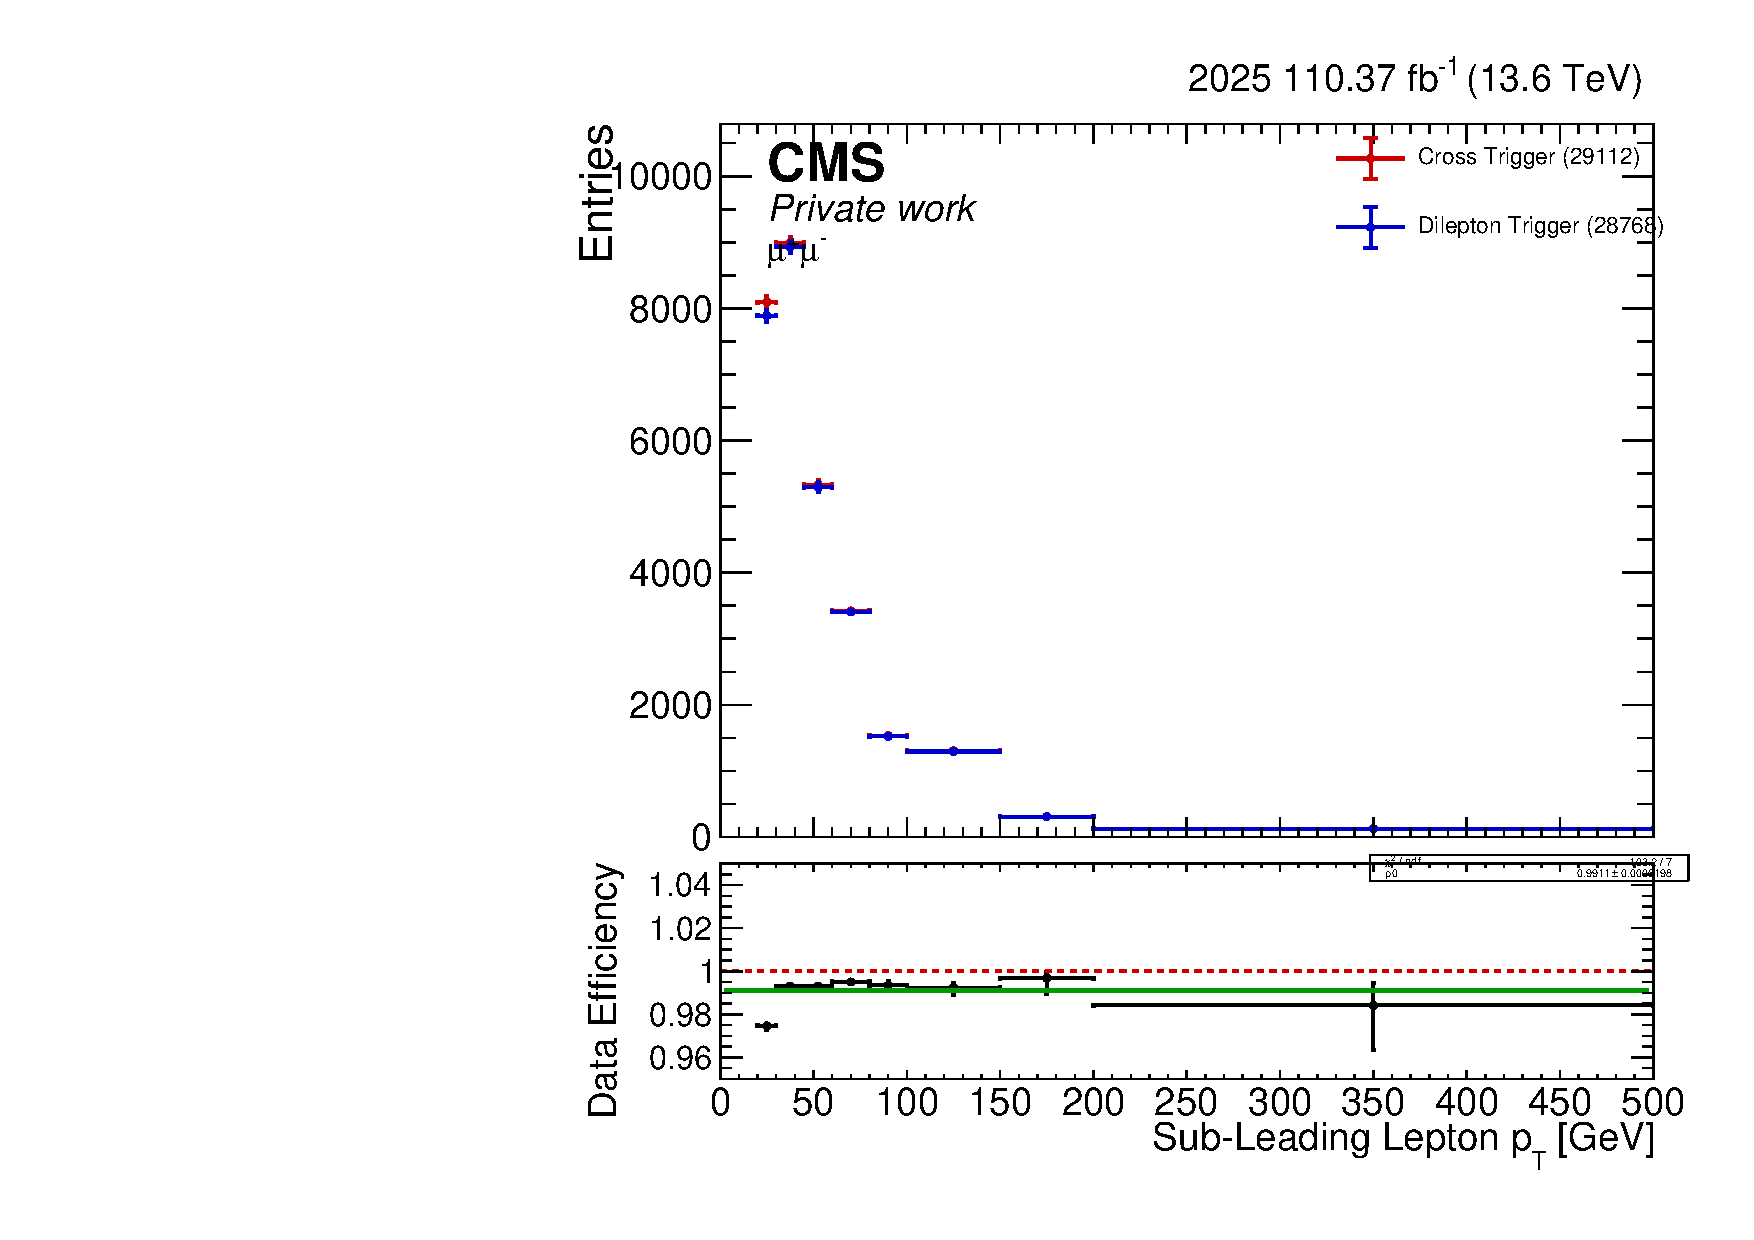
\includegraphics[width=0.48\linewidth]{figures/2025/MuMu/TrigEffData/TrigEff_Lep2pt.pdf}
\caption{Data trigger numerator and reference-sample distributions (upper panels), with their efficiency ratios (lower panels) in the $\mu\mu$ channel. Left and right: leading and subleading lepton $p_{\mathrm{T}}$.}\label{fig:extra-MuMu-TrigEffData-Lep1pt-2025}\end{figure}
\begin{figure}[p]\centering
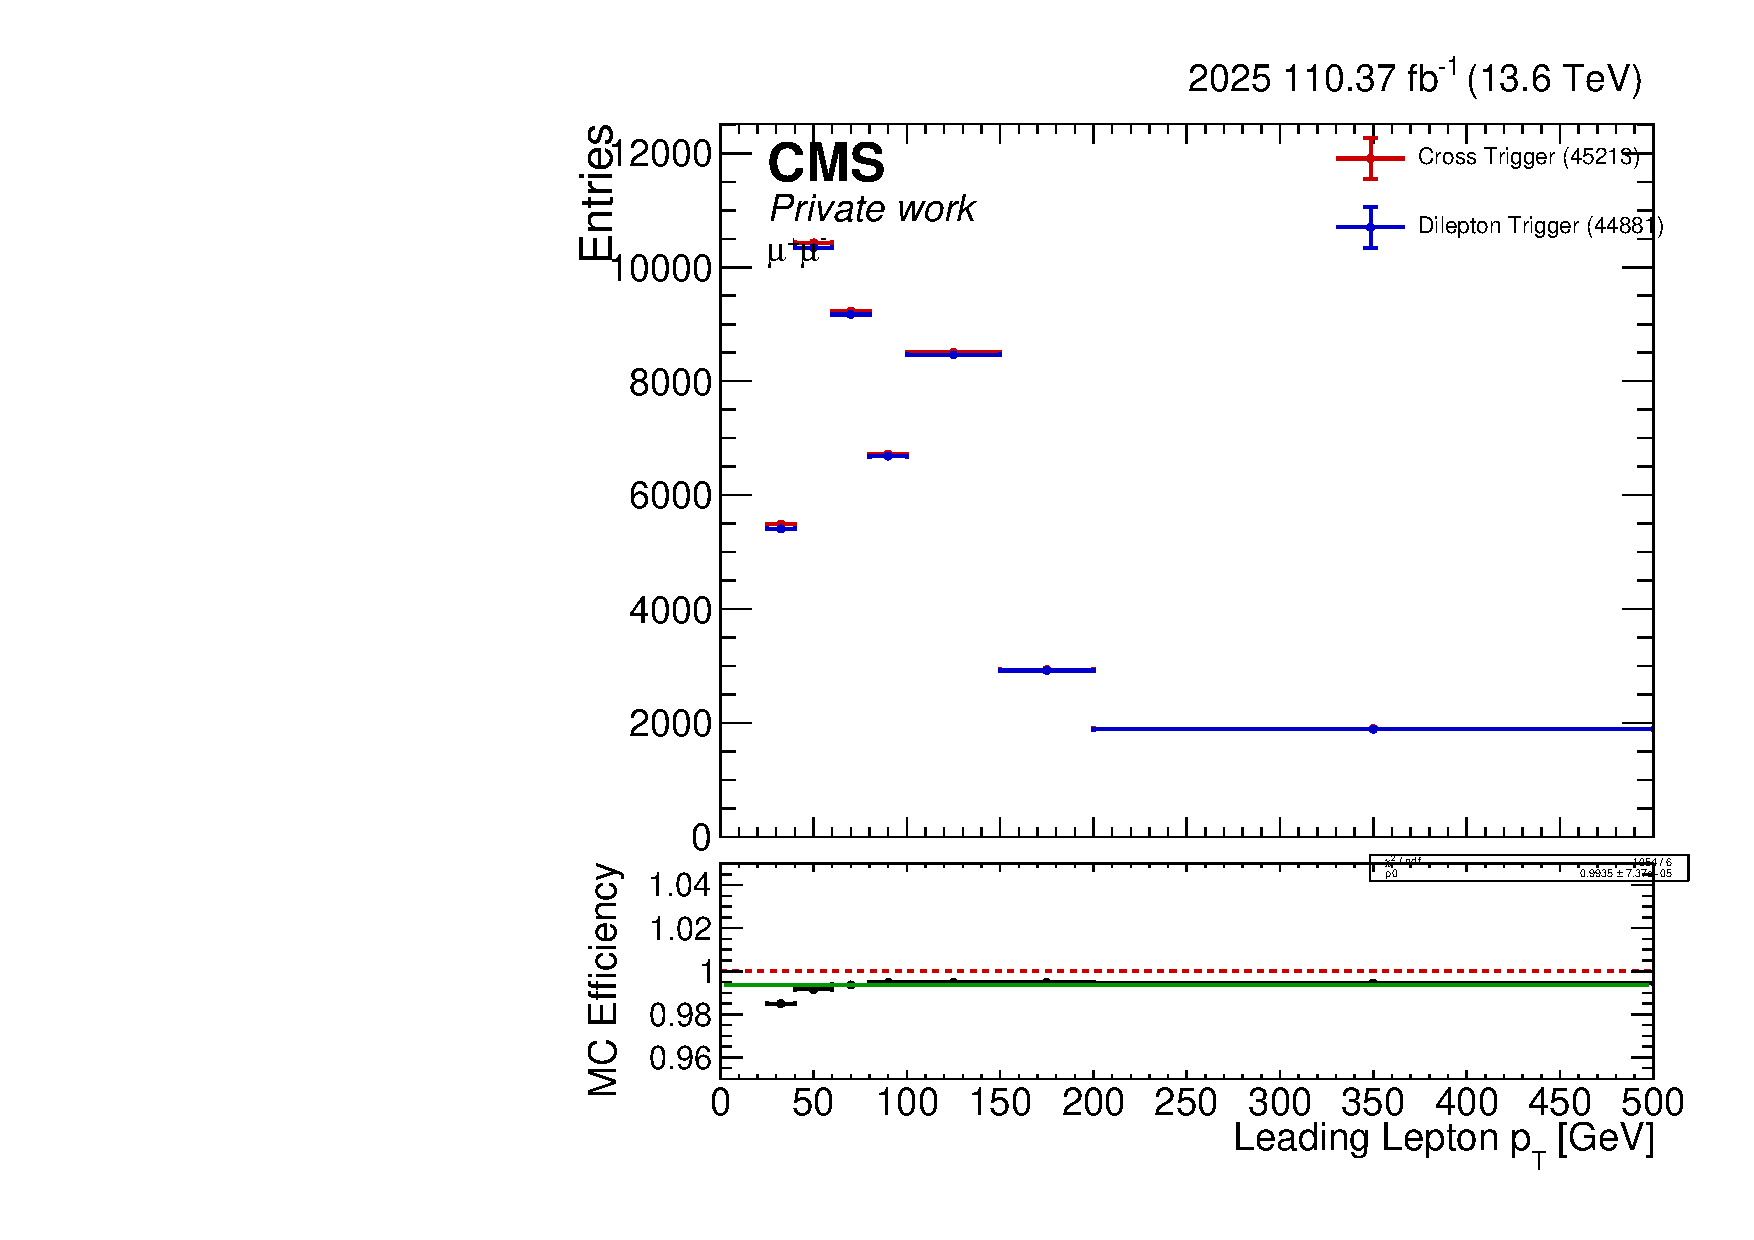
\includegraphics[width=0.48\linewidth]{figures/2025/MuMu/TrigEffMC/TrigEff_Lep1pt.pdf}
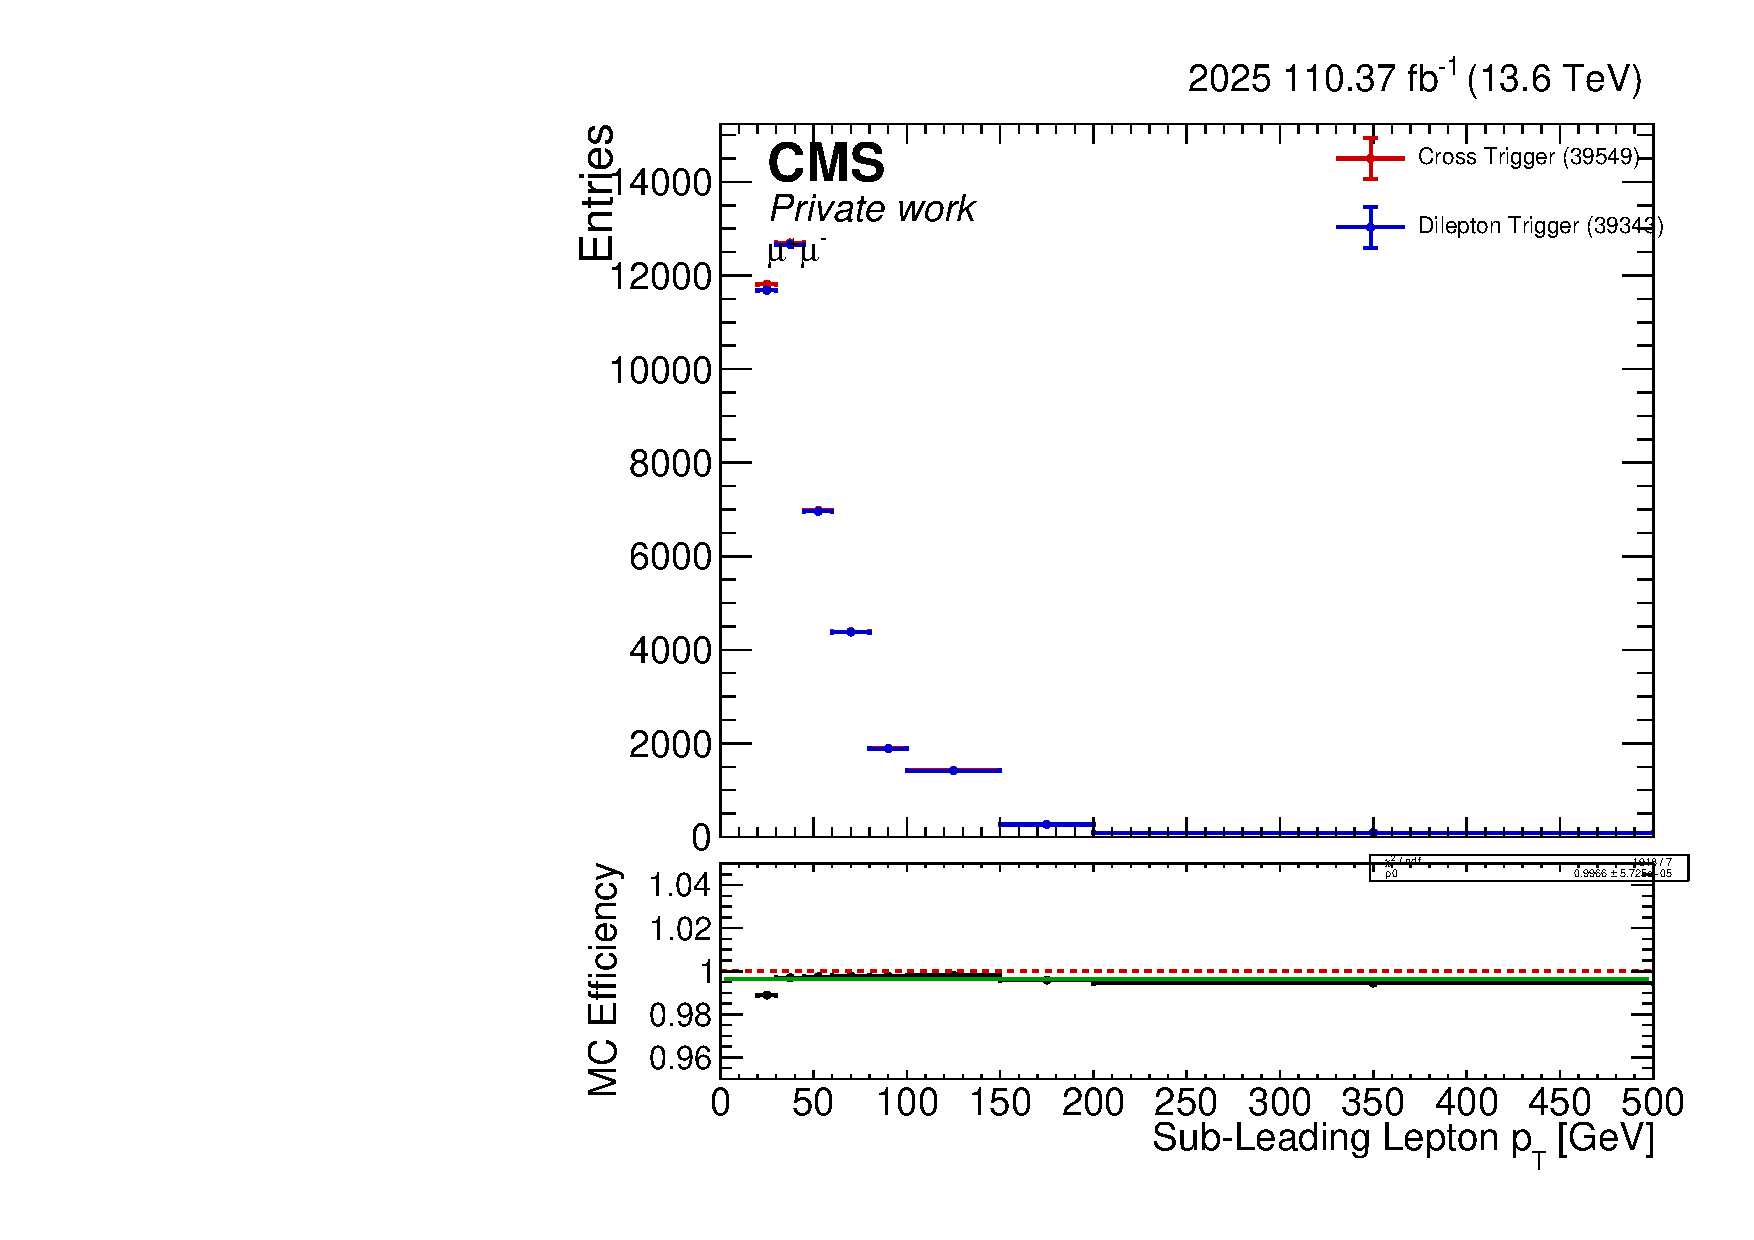
\includegraphics[width=0.48\linewidth]{figures/2025/MuMu/TrigEffMC/TrigEff_Lep2pt.pdf}
\caption{Simulated trigger numerator and reference-sample distributions (upper panels), with their efficiency ratios (lower panels) in the $\mu\mu$ channel. Left and right: leading and subleading lepton $p_{\mathrm{T}}$.}\label{fig:extra-MuMu-TrigEffMC-Lep1pt-2025}\end{figure}
\begin{figure}[p]\centering
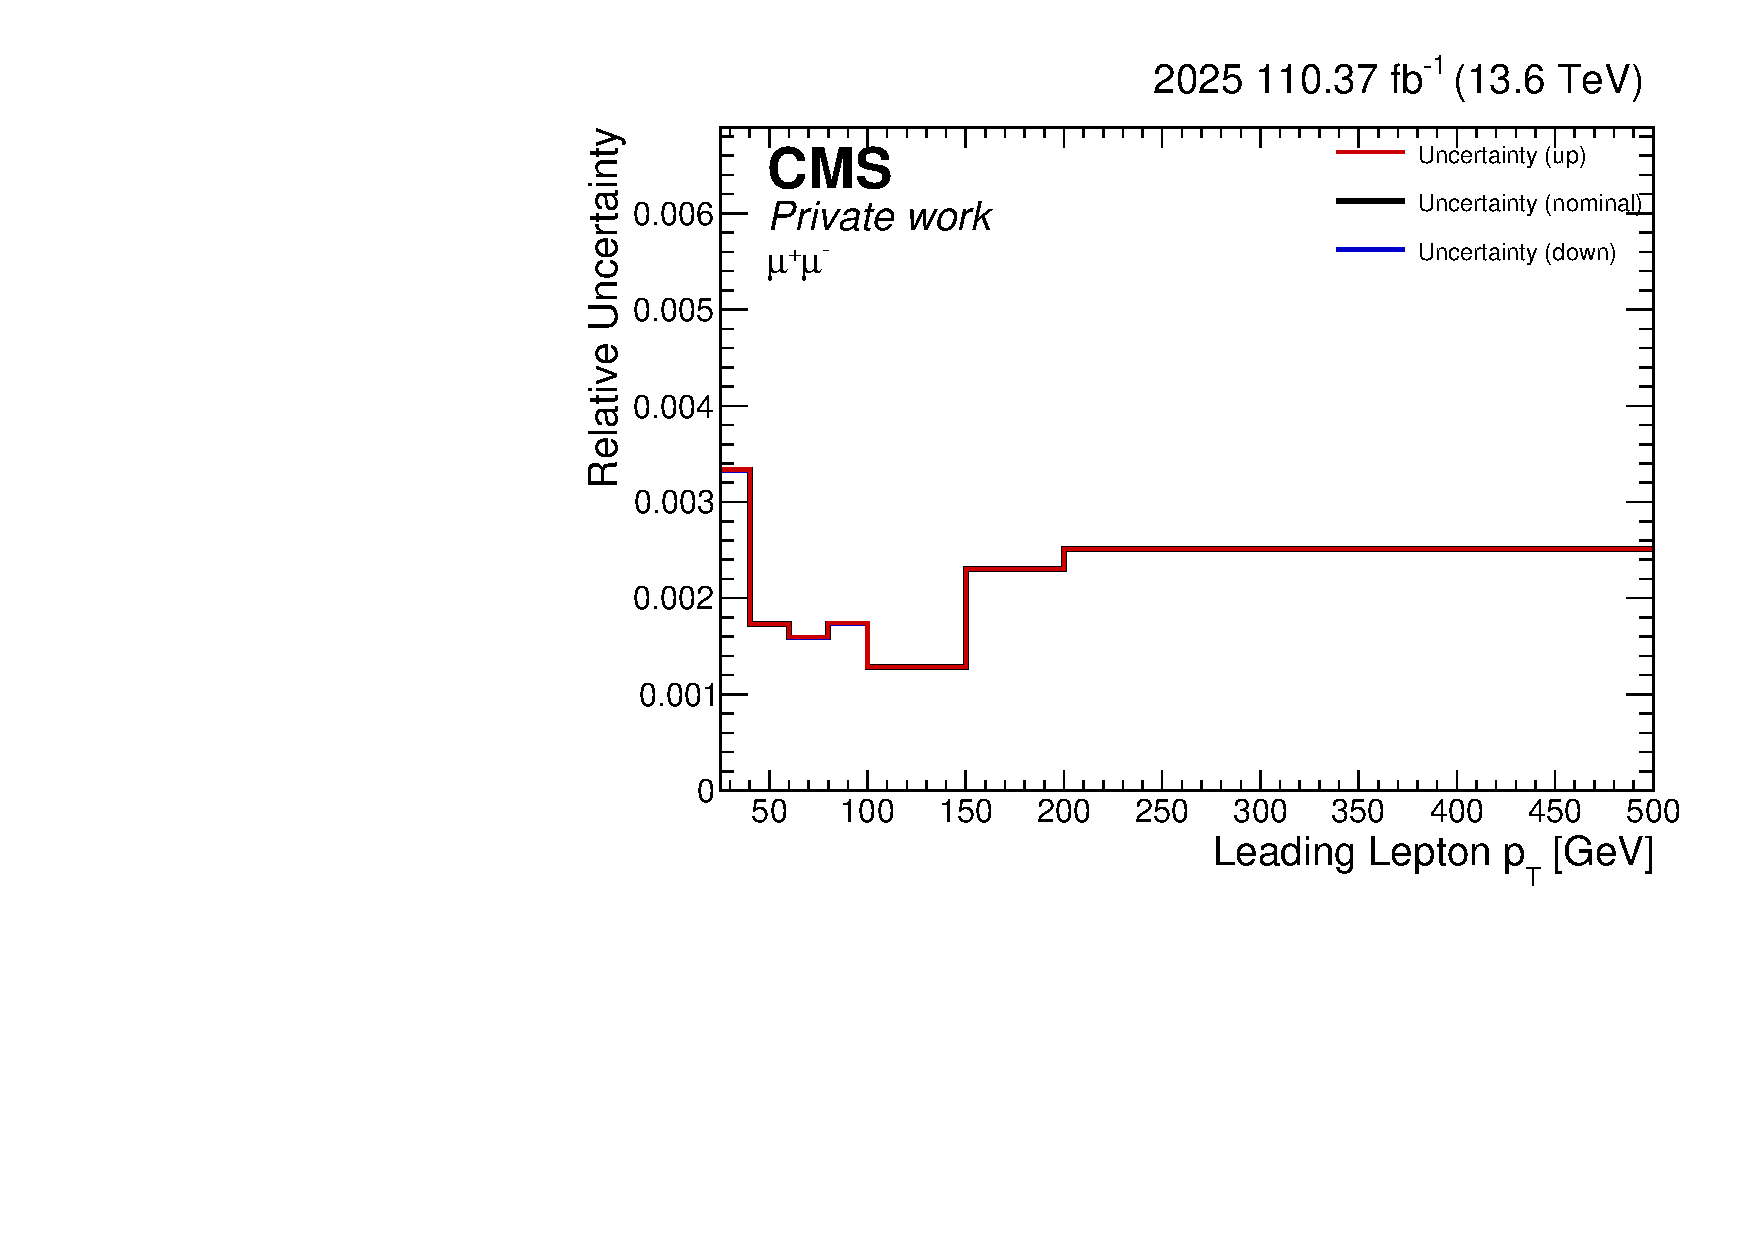
\includegraphics[width=0.48\linewidth]{figures/2025/MuMu/Statistical_Uncertainty/UncRatio_Lep1pt.pdf}
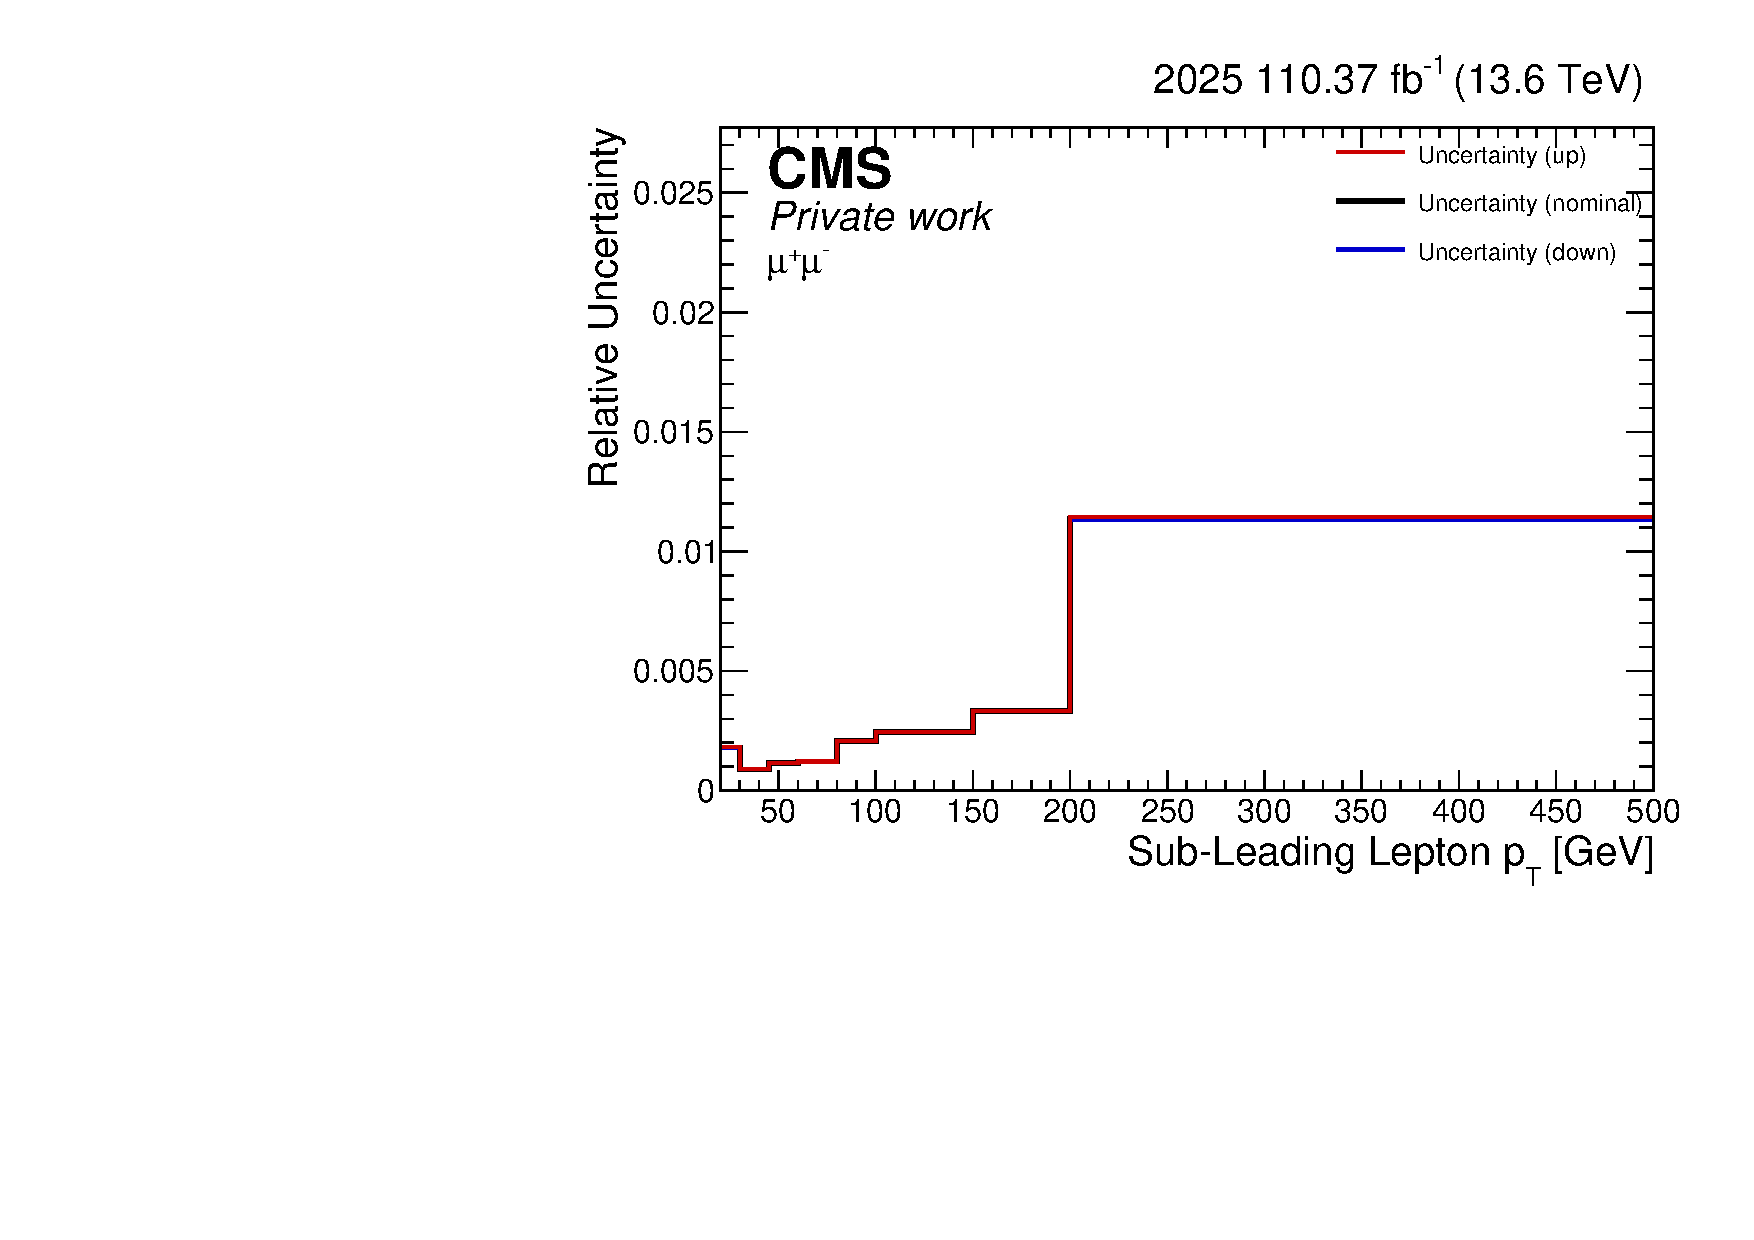
\includegraphics[width=0.48\linewidth]{figures/2025/MuMu/Statistical_Uncertainty/UncRatio_Lep2pt.pdf}
\caption{Relative statistical uncertainty diagnostics, retaining the nominal, upward, and downward curves of the supplied production in the $\mu\mu$ channel. Left and right: leading and subleading lepton $p_{\mathrm{T}}$.}\label{fig:extra-MuMu-Statistical-Uncertainty-Lep1pt-2025}\end{figure}
\begin{figure}[p]\centering
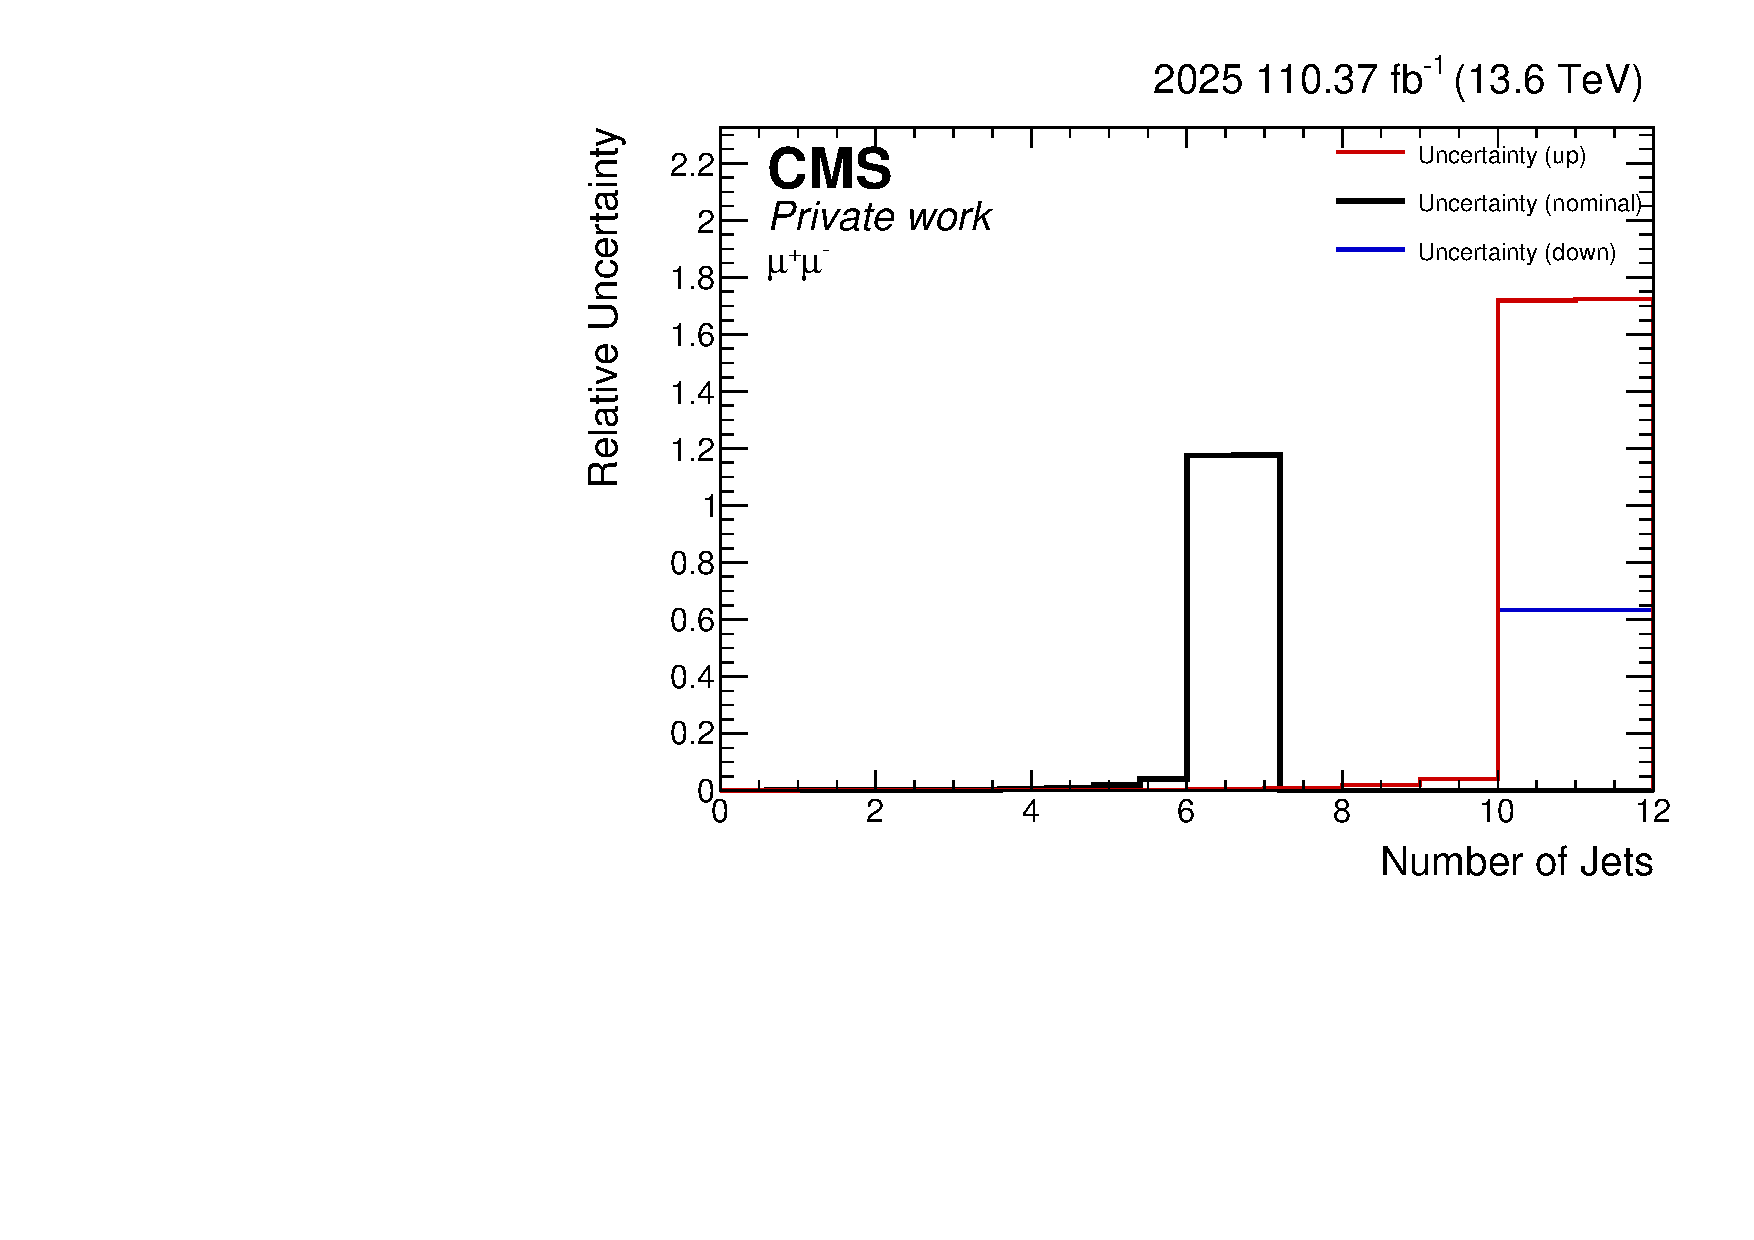
\includegraphics[width=0.48\linewidth]{figures/2025/MuMu/Statistical_Uncertainty/UncRatio_Num_Jets.pdf}
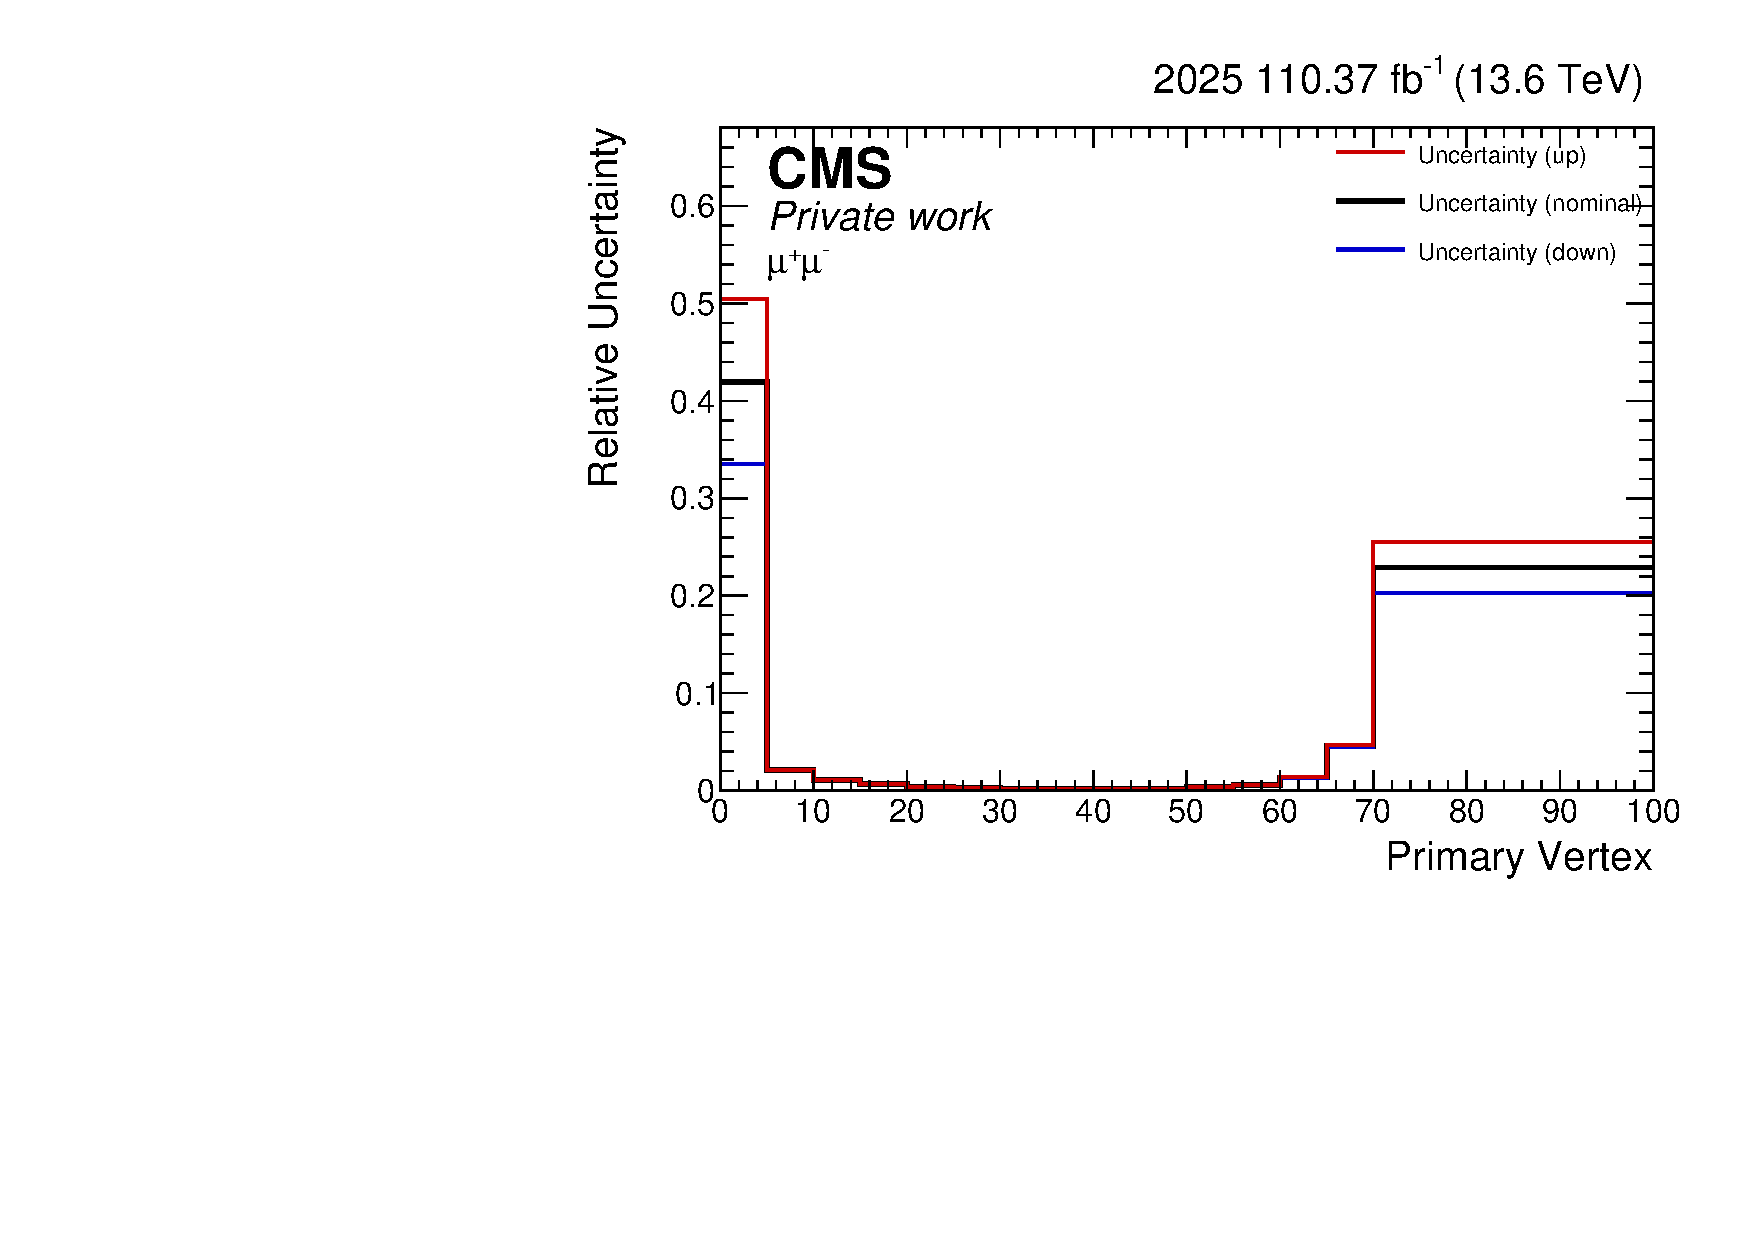
\includegraphics[width=0.48\linewidth]{figures/2025/MuMu/Statistical_Uncertainty/UncRatio_Num_PV.pdf}
\caption{Relative statistical uncertainty diagnostics, retaining the nominal, upward, and downward curves of the supplied production in the $\mu\mu$ channel. Left and right: jet and primary-vertex multiplicities.}\label{fig:extra-MuMu-Statistical-Uncertainty-Num_Jets-2025}\end{figure}
\begin{figure}[p]\centering
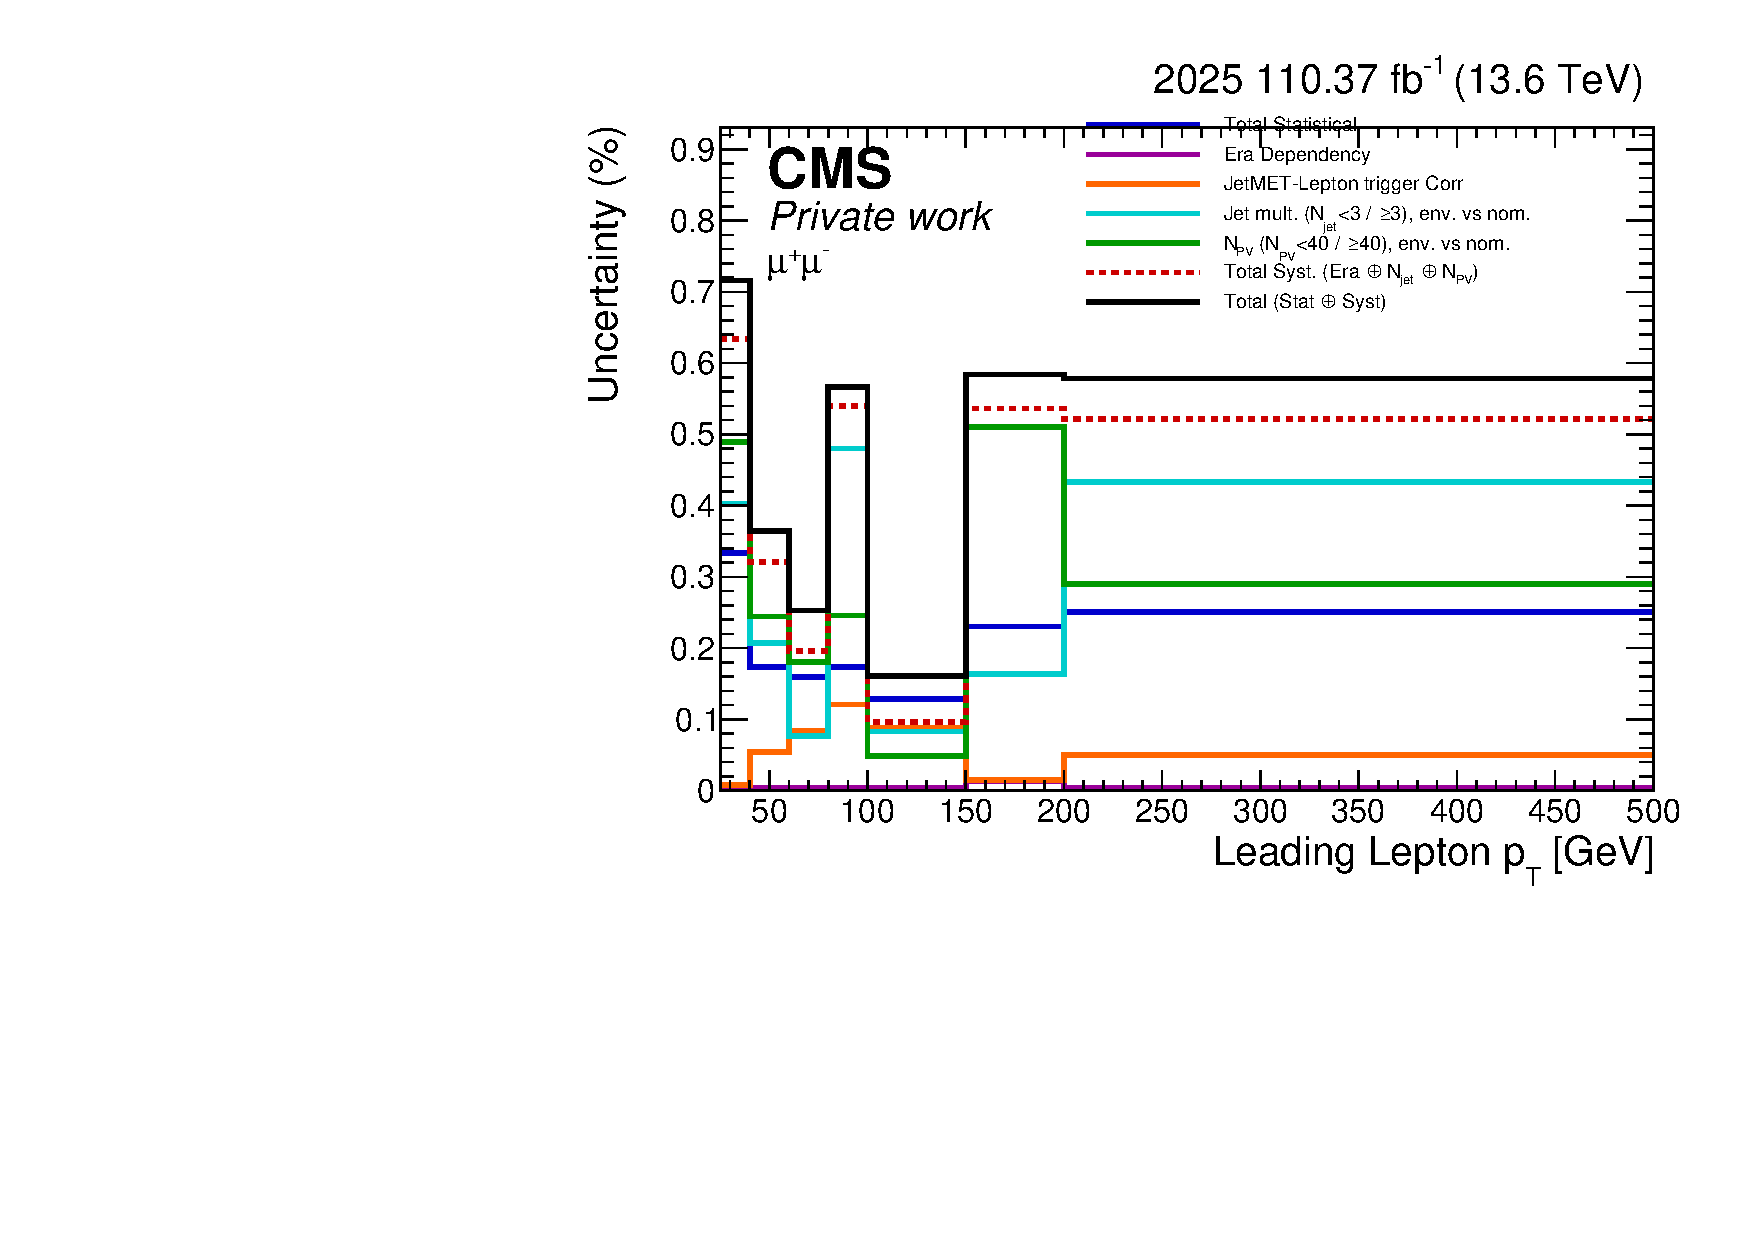
\includegraphics[width=0.48\linewidth]{figures/2025/MuMu/Uncertainty_Breakdown/Breakdown_Lep1pt.pdf}
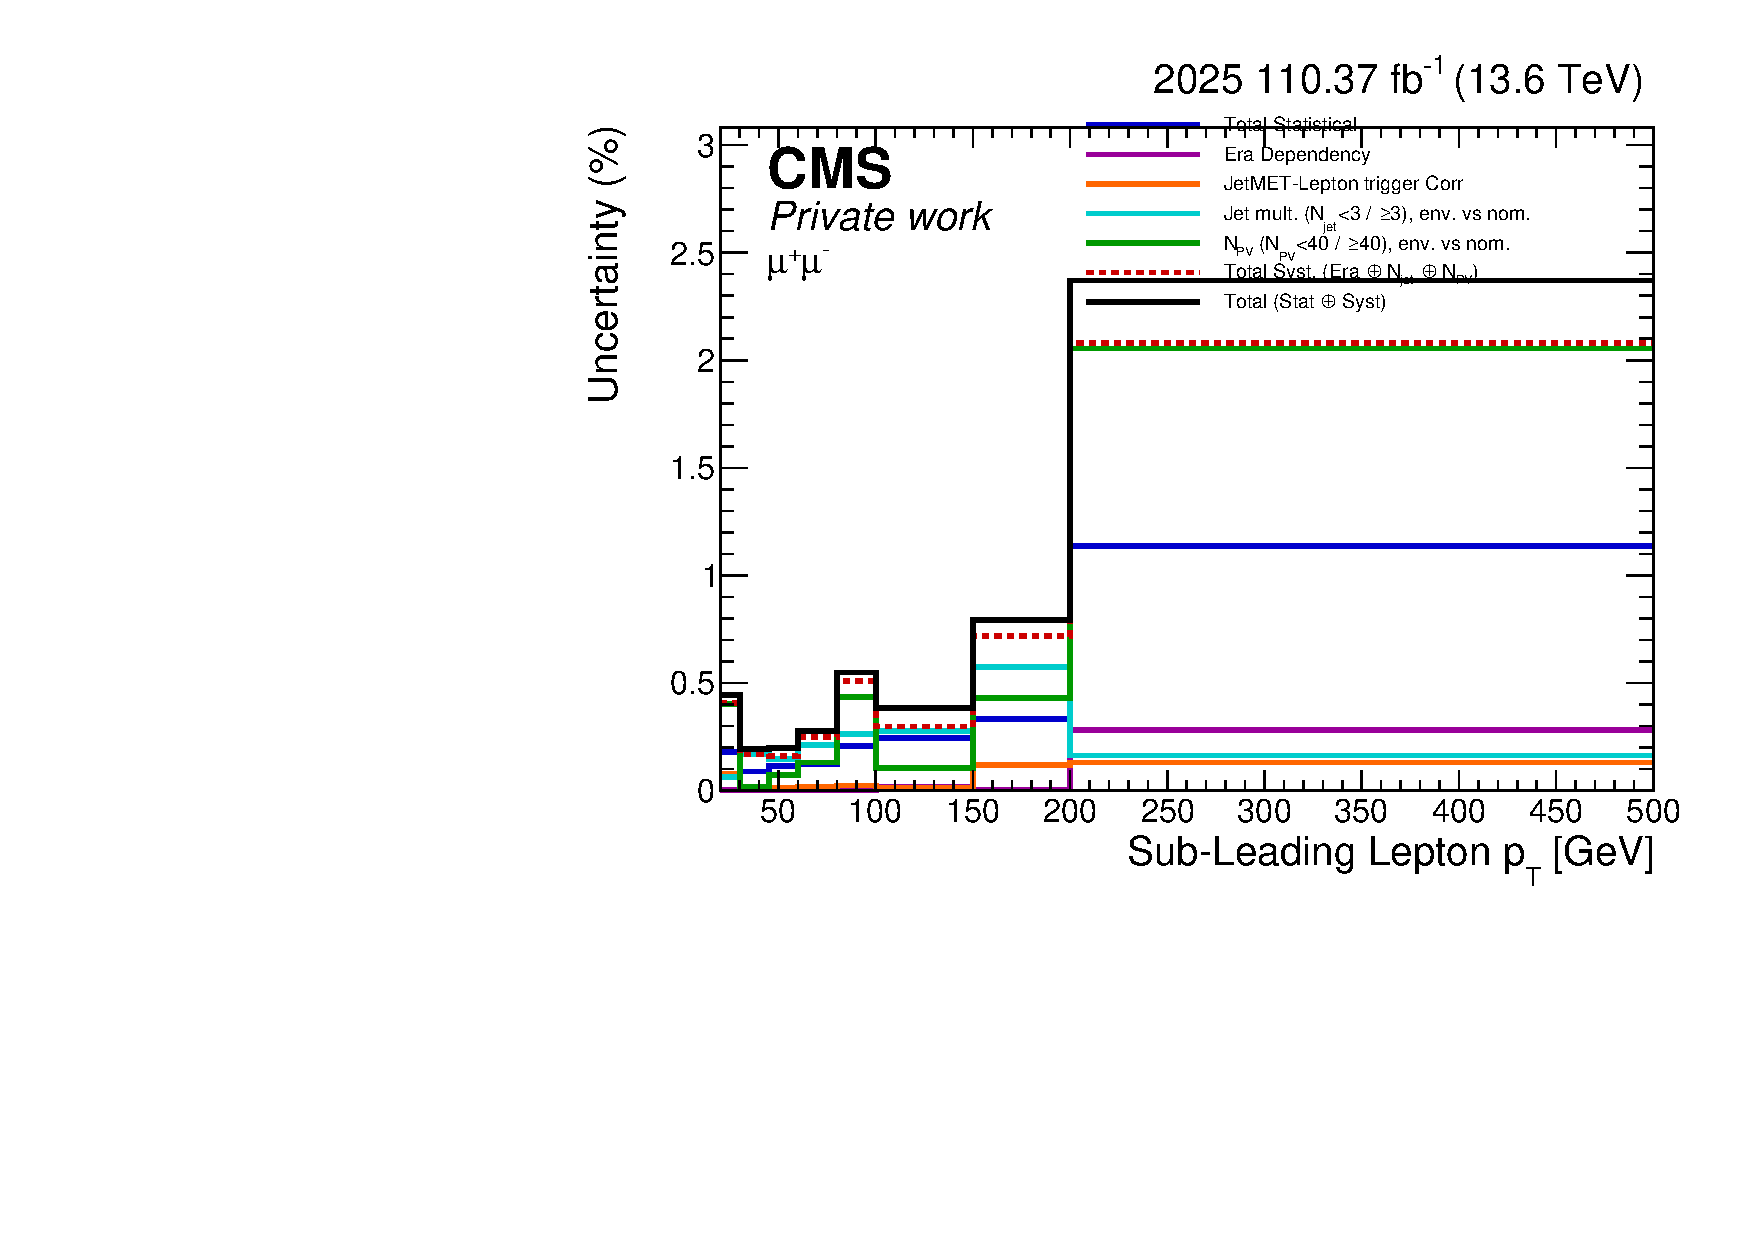
\includegraphics[width=0.48\linewidth]{figures/2025/MuMu/Uncertainty_Breakdown/Breakdown_Lep2pt.pdf}
\caption{Absolute uncertainty component breakdown in the $\mu\mu$ channel. Left and right: leading and subleading lepton $p_{\mathrm{T}}$.}\label{fig:extra-MuMu-Uncertainty-Breakdown-Lep1pt-2025}\end{figure}
\begin{figure}[p]\centering
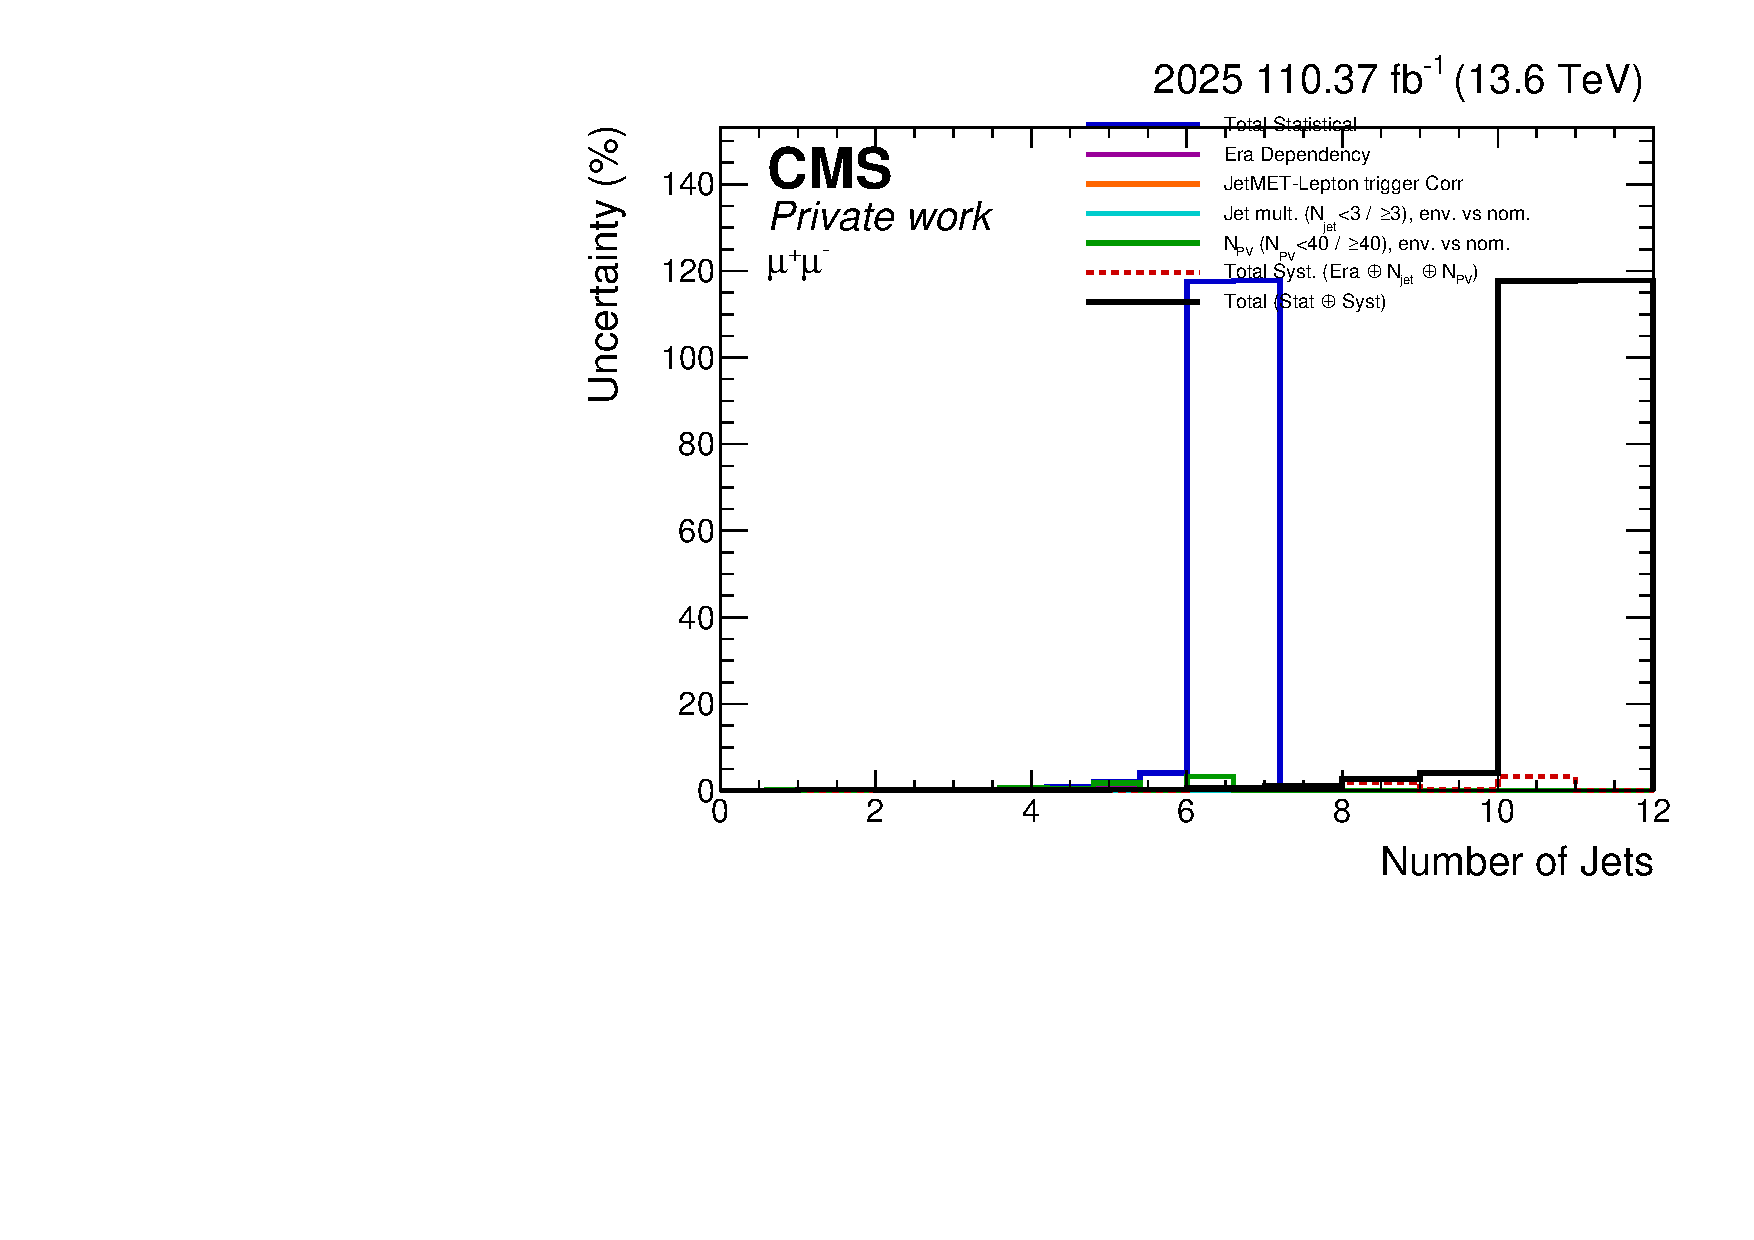
\includegraphics[width=0.48\linewidth]{figures/2025/MuMu/Uncertainty_Breakdown/Breakdown_Num_Jets.pdf}
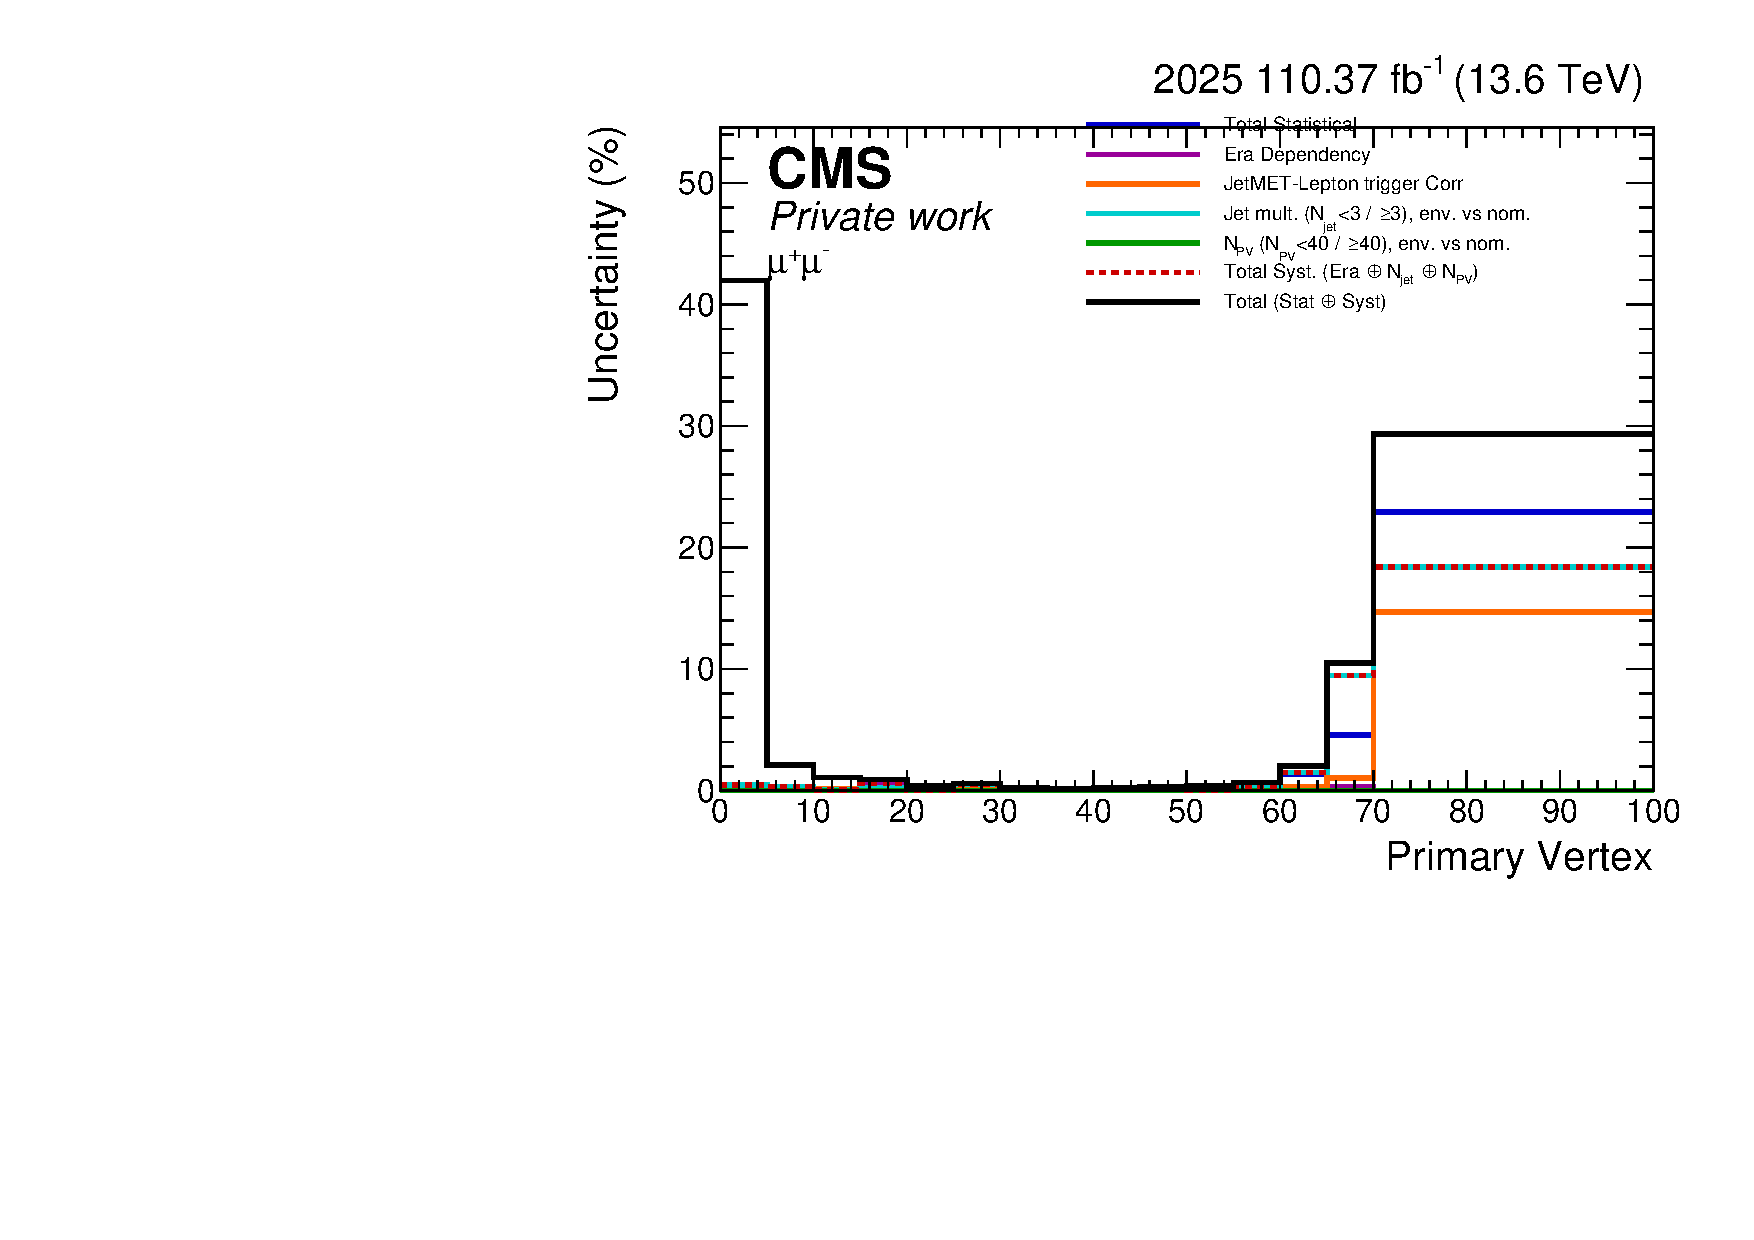
\includegraphics[width=0.48\linewidth]{figures/2025/MuMu/Uncertainty_Breakdown/Breakdown_Num_PV.pdf}
\caption{Absolute uncertainty component breakdown in the $\mu\mu$ channel. Left and right: jet and primary-vertex multiplicities.}\label{fig:extra-MuMu-Uncertainty-Breakdown-Num_Jets-2025}\end{figure}
\begin{figure}[p]\centering
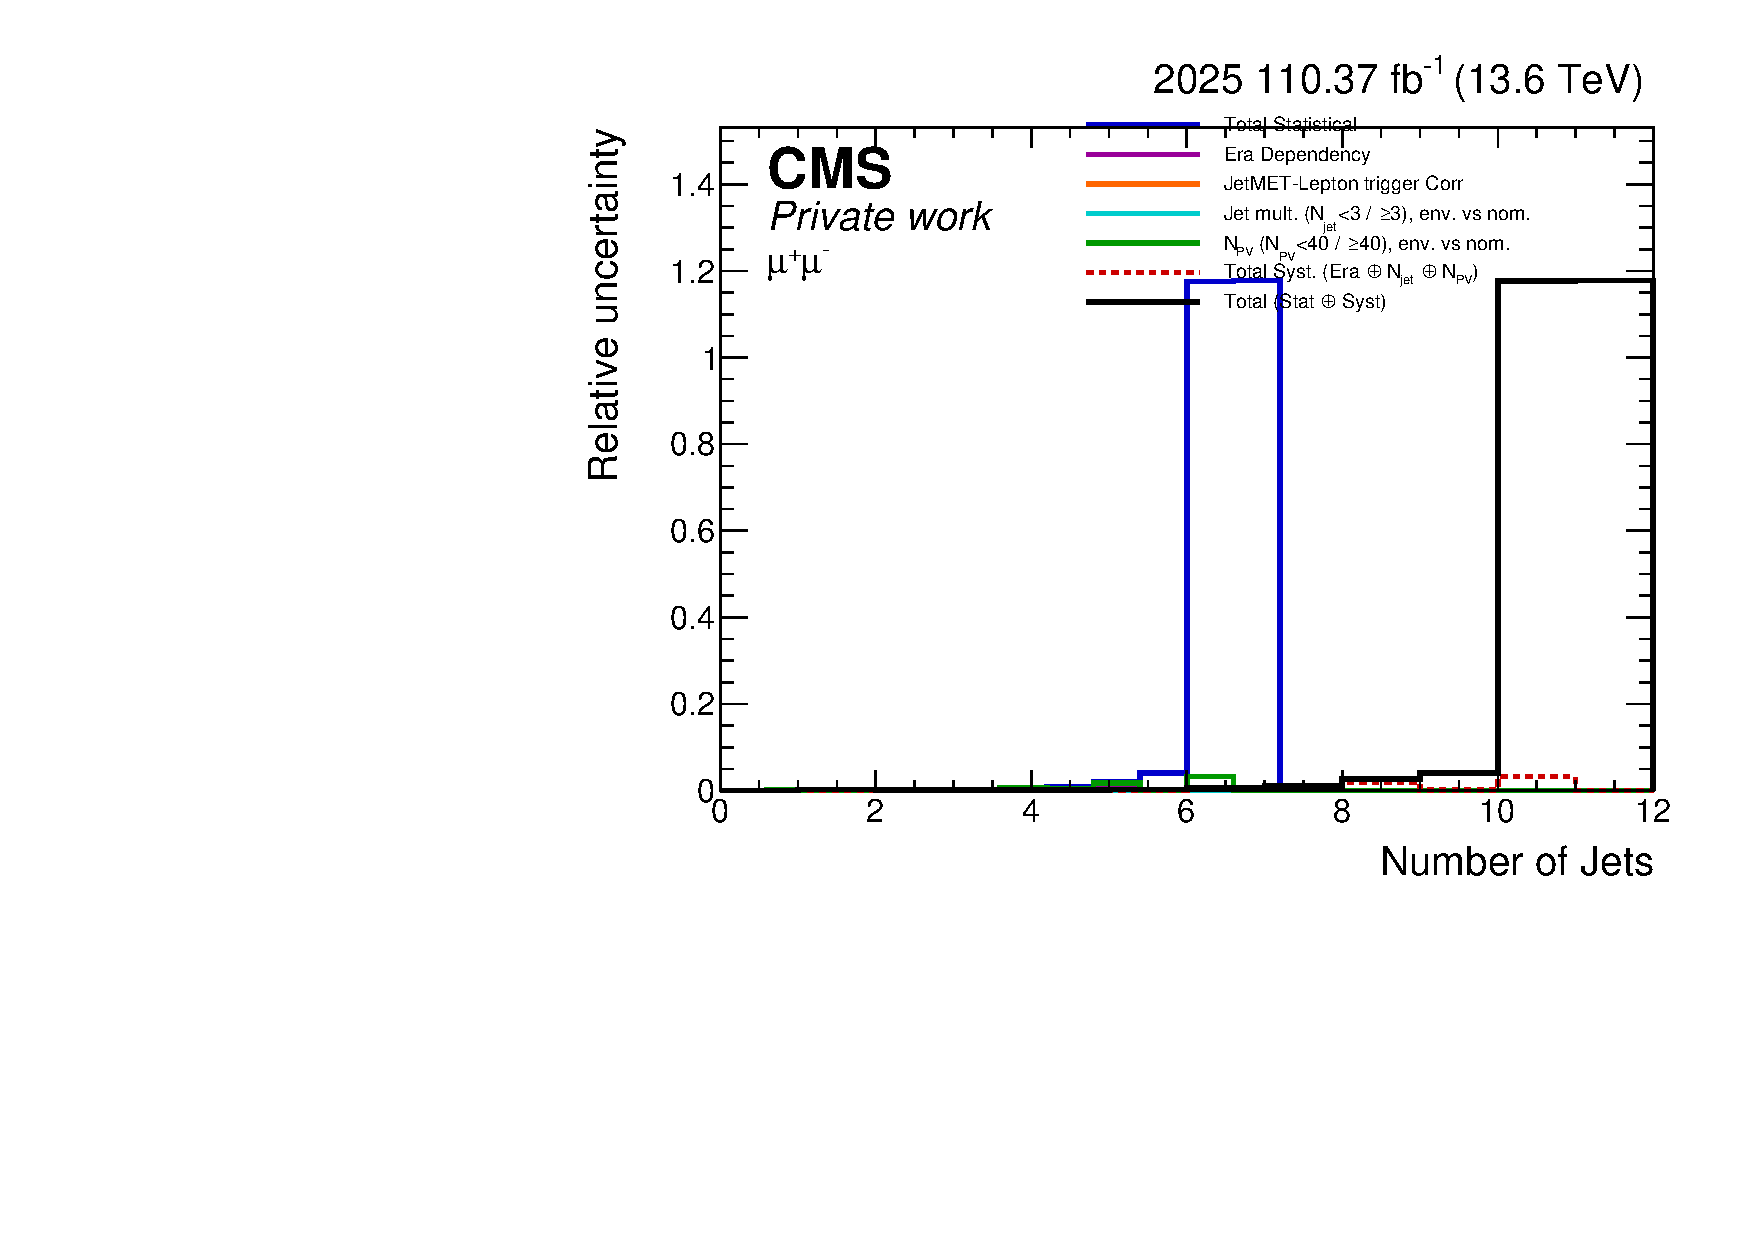
\includegraphics[width=0.48\linewidth]{figures/2025/MuMu/Relative_Uncertainty_Breakdown/Breakdown_Num_Jets.pdf}
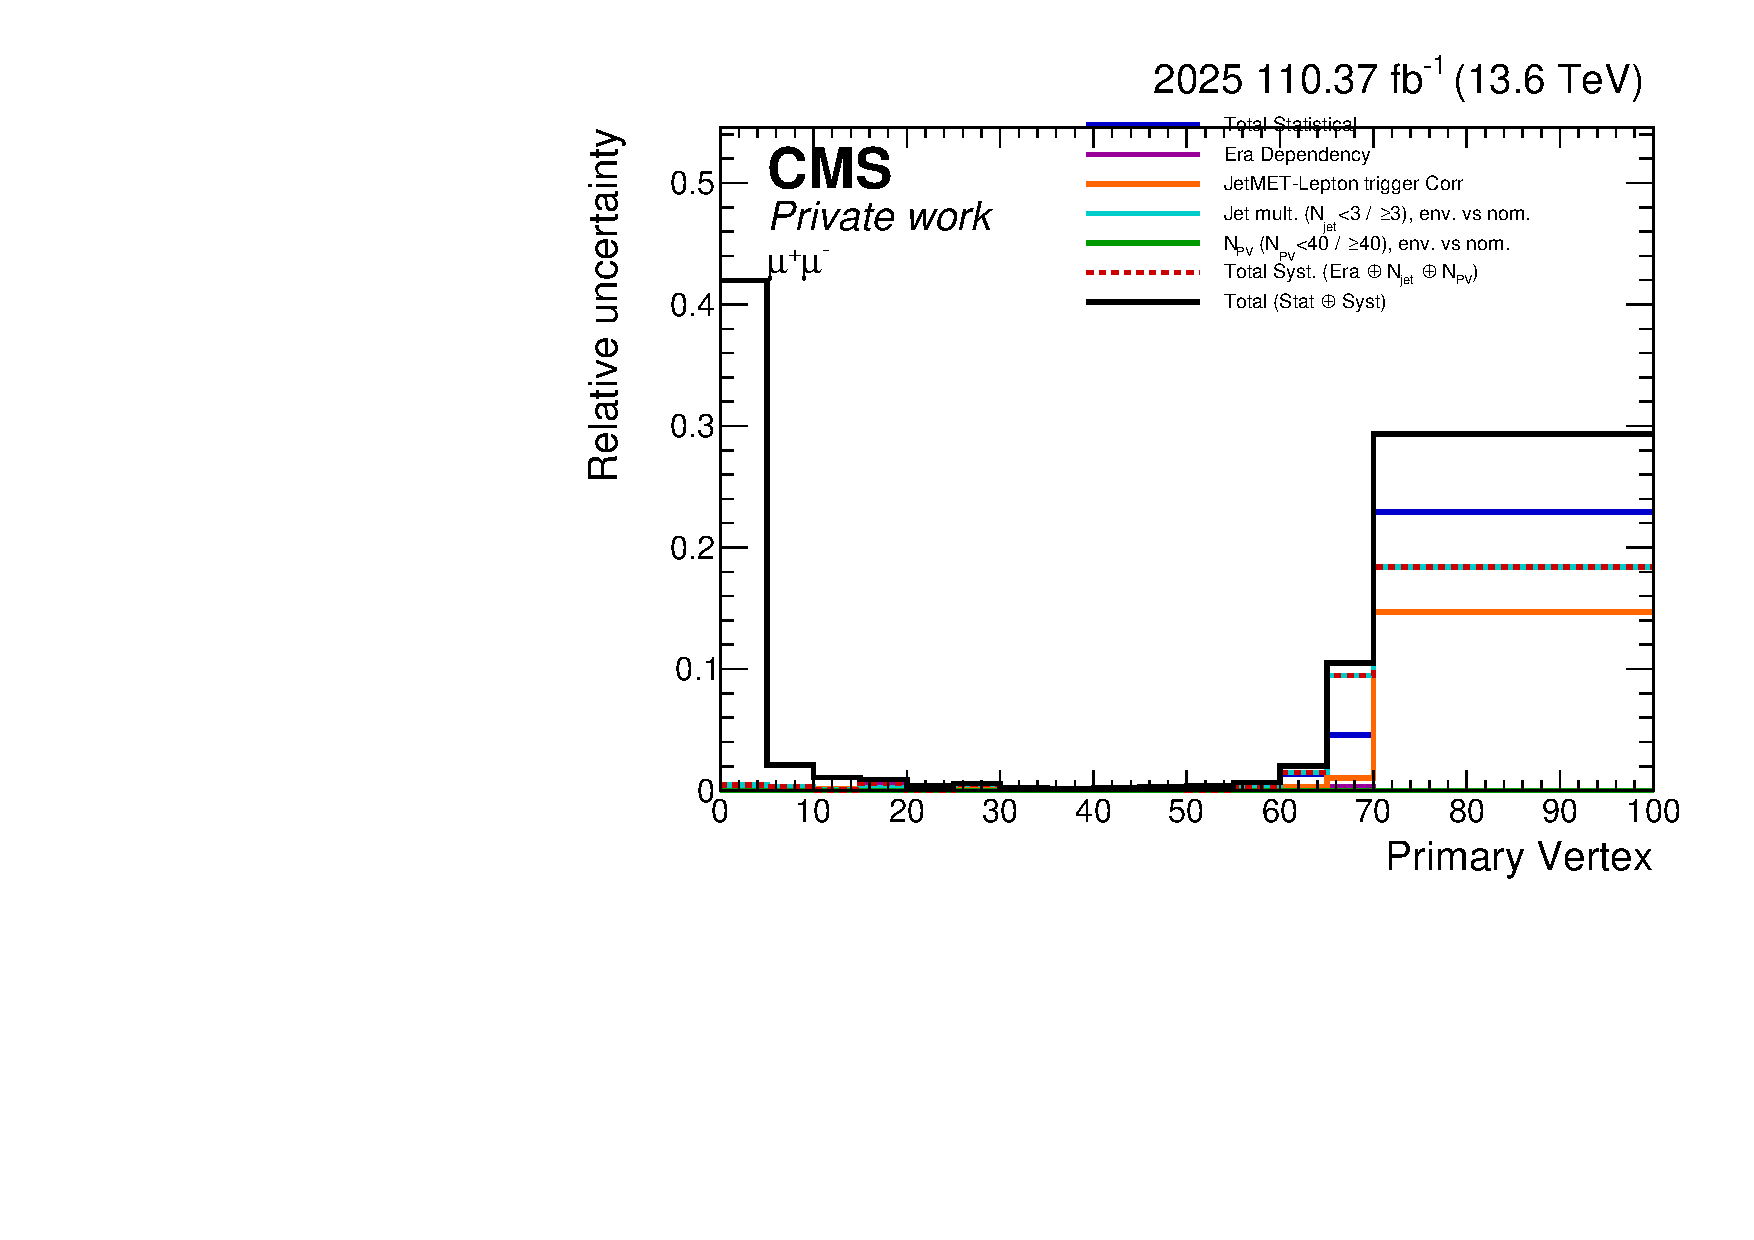
\includegraphics[width=0.48\linewidth]{figures/2025/MuMu/Relative_Uncertainty_Breakdown/Breakdown_Num_PV.pdf}
\caption{Relative uncertainty component breakdown versus event activity in the $\mu\mu$ channel. Left and right: jet and primary-vertex multiplicities.}\label{fig:extra-MuMu-Relative-Uncertainty-Breakdown-Num_Jets-2025}\end{figure}
\begin{figure}[p]\centering
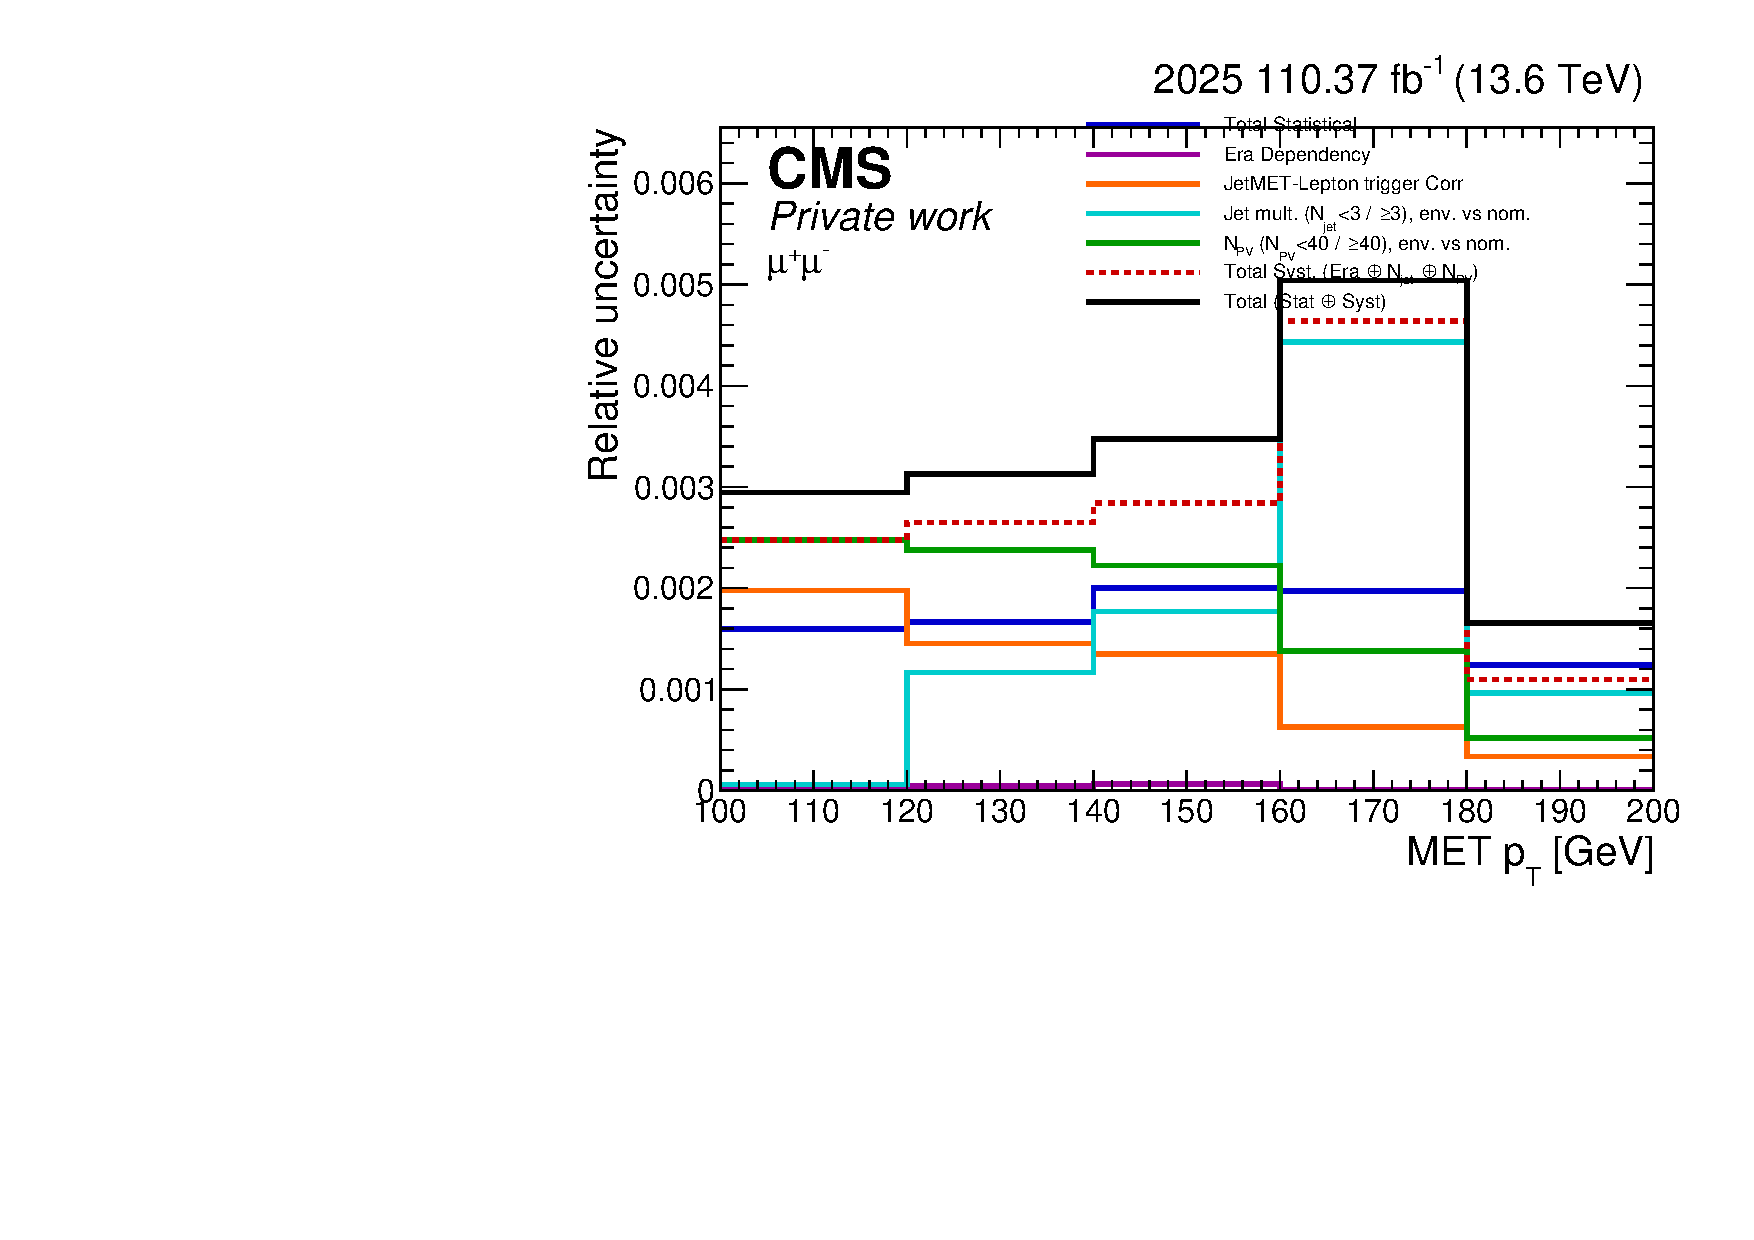
\includegraphics[width=0.48\linewidth]{figures/2025/MuMu/Relative_Uncertainty_Breakdown/Breakdown_METpt.pdf}
\includegraphics[width=0.48\linewidth]{figures/2025/MuMu/Relative_Uncertainty_Breakdown/Breakdown_DiLepMass.pdf}
\caption{Relative uncertainty component breakdown versus event kinematics in the $\mu\mu$ channel. Left and right: missing transverse momentum and dilepton invariant mass.}\label{fig:extra-MuMu-Relative-Uncertainty-Breakdown-METpt-2025}\end{figure}
\begin{figure}[p]\centering
\includegraphics[width=0.48\linewidth]{figures/2025/MuMu/ScaleFactor/SF_Num_bJets.pdf}
\caption{Efficiency comparison and scale factor versus heavy-flavour activity in the $\mu\mu$ channel. $b$-tagged jet multiplicity.}\label{fig:extra-MuMu-ScaleFactor-Num_bJets-2025}\end{figure}


